% Generated deterministically by scripts/build_partial_epub3.py.
% Inclusion authority: alignment/UNITS.jsonl sha256=d560f9def1e305991719be75df5397e9514b7768ca8fd40bbe5ac9a0c4d336c2
% Accepted contiguous prefix: OLP-0001--OLP-0192 (192 units).
% First excluded unit: OLP-0193.
% This cumulative file contains every accepted source body inline.  It does
% not follow source driver imports and therefore cannot include pending units.
\documentclass[openany]{memoir}
\newcommand*{\olpath}{upstream}
\newcommand*{\ollangid}{nl}
\newcommand*{\ollanguage}{dutch}
\usepackage[T1]{fontenc}
\usepackage[utf8]{inputenc}
\usepackage{mathpazo}
\usepackage{helvet}
\usepackage{courier}
\linespread{1.05}
\setlength{\emergencystretch}{1em}
\input{upstream/sty/open-logic.sty}
\input{upstream/sty/open-logic-defer.sty}
\includeenv{editorial}
\problemsperchapter
\let\cleardoublepage\clearpage
\hypersetup{
  unicode=true,
  pdflang={nl-NL},
  pdftitle={The Open Logic Text --- gedeeltelijke Nederlandstalige editie (gewoon register)},
  pdfauthor={The Open Logic Project en vermelde medewerkers},
  pdfsubject={Gedeeltelijke reader met uitsluitend de geaccepteerde aaneengesloten prefix OLP-0001--OLP-0192},
  pdfkeywords={logica, verzamelingenleer, Nederlandse vertaling, gedeeltelijke editie}
}
\begin{document}
\begin{titlingpage}
\begin{raggedleft}
\HUGE\selectfont\bfseries\sffamily The Open Logic Text
\vskip 3ex
\normalfont\huge Gedeeltelijke Nederlandstalige editie\\
\Large gewoon register
\vskip 4ex
\large Geaccepteerde broneenheden OLP-0001--OLP-0192\\
2026-09-27
\end{raggedleft}
\vfill
\noindent Gebaseerd op het Open Logic Project. De tekst en broncode worden
beschikbaar gesteld onder Creative Commons Naamsvermelding 4.0 Internationaal.
\end{titlingpage}
\chapter*{Reikwijdte van deze gedeeltelijke editie}
\addcontentsline{toc}{chapter}{Reikwijdte van deze gedeeltelijke editie}
Deze editie bevat uitsluitend de 192 opeenvolgende,
in \texttt{alignment/UNITS.jsonl} geaccepteerde broneenheden OLP-0001--OLP-0192.
Broneenheid OLP-0193 en alle latere eenheden zijn niet opgenomen.
Een vertaalbestand dat al bestaat maar nog niet als geaccepteerd is gemarkeerd,
maakt uitdrukkelijk geen deel uit van deze editie. Het laatste hoofdstuk kan
daardoor inhoudelijk onvolledig zijn; dat is een eigenschap van deze begrensde
editie en geen claim dat het volledige Open Logic Text al vertaald is.
\chapter*{Status en verantwoording}
\addcontentsline{toc}{chapter}{Status en verantwoording}
Dit is een gedeeltelijke reader: 192 van de 722
broneenheden, in het gewoon register. De termen
``geaccepteerd'' en ``gecontroleerd'' verwijzen naar de vastgelegde
AI-productiecontroles, niet naar onafhankelijk deskundigenonderzoek.

Vertaling en eerdere controles: OpenAI Codex; de huidige eigenaar gebruikt GPT-5.6 Sol, Ultra effort. De exacte historische model- en inspanningsinstelling van ieder tekstgedeelte zijn nog niet afzonderlijk bewezen; de huidige instelling wordt daarom niet aan alle eerdere vertaalbytes toegeschreven. Samenstelling van deze reader, directe EPUB-conversie en deterministische bouwcontroles: OpenAI Codex — GPT-5.6 Sol, Ultra effort. Geen menselijke redactie of beoordeling wordt geclaimd.
\tableofcontents*

% BEGIN ACCEPTED UNIT OLP-0001 path=translations/nl-gewoon/content/open-logic-about.tex source-sha256=4567f54b1ddebcdc856036e0852da78e0135aa5092544e8825750ad1d89ede08
\begingroup
\def\olfilename{OLP-0001}
\def\olfilepath{content/}
\hypertarget{unit-OLP-0001}{}
\typeout{PARTIAL-READER-UNIT OLP-0001}
% BEGIN ACCEPTED BODY OLP-0001 body-sha256=4567f54b1ddebcdc856036e0852da78e0135aa5092544e8825750ad1d89ede08
\chapter*{Over het Open Logic Project}
\addcontentsline{toc}{chapter}{Over het Open Logic Project}


De \textit{Open Logic Text} is een opensourceleerboek waaraan mensen samen
schrijven. Het gaat over formele
metalogica, dus over het onderzoek naar formele logische systemen, en over
formele methoden. Het boek begint niet bij nul:
het gaat ervan uit dat je al een inleidende cursus formele logica hebt gevolgd.
Het boek is bedoeld voor lezers buiten de wiskunde, met name voor studenten
filosofie en informatica. Toch behandelt het de stof wiskundig precies.

Sommige onderwerpen staan al in het boek, maar zijn misschien nog niet
volledig behandeld. Veel stukken moeten nog flink worden herzien. We zijn van
plan het boek later met meer onderwerpen uit te breiden. Ook zijn we van plan
onderdelen aan het boek toe te voegen, bijvoorbeeld een woordenlijst, een lijst
met tips voor wat je verder kunt lezen, uitleg over de geschiedenis,
afbeeldingen en betere uitleg. Verder zijn we van plan stukken toe te voegen
waarin we uitleggen waarom de resultaten belangrijk zijn voor filosofie,
informatica en wiskunde, en meer opgaven en voorbeelden.
Zie je een fout of heb je een voorstel,
\href{https://github.com/OpenLogicProject/OpenLogic/wiki/Contributing}{laat het projectteam dat dan weten}.

Het project werkt volgens het idee van open source. De tekst is niet alleen
vrij beschikbaar; we geven ook de LaTeX-broncode vrij onder de licentie
Creative Commons Naamsvermelding. Volgens die licentie mag iedereen ons werk
downloaden, gebruiken, aanpassen, anders indelen, omzetten en verder
verspreiden, zolang de makers op de juiste manier worden genoemd. Meer
informatie staat op de website van het
Open Logic Project: \href{http://openlogicproject.org/}{openlogicproject.org}.
% END ACCEPTED BODY OLP-0001
\endgroup
% END ACCEPTED UNIT OLP-0001

% BEGIN ACCEPTED UNIT OLP-0002 path=translations/nl-gewoon/content/content.tex source-sha256=e1e279f0ce60c408900d570b801b2b0948e47777c2fe682d30225e3390e83525
\begingroup
\def\olfilename{OLP-0002}
\def\olfilepath{content/}
\hypertarget{unit-OLP-0002}{}
\typeout{PARTIAL-READER-UNIT OLP-0002}
% BEGIN ACCEPTED BODY OLP-0002 body-sha256=395f9476d78095c654301f15949603246ae6d9d59733bd6a1c97b950cc28d5e1
% open-logic.tex
% compiles to produce complete text using open-logic-dev style



\clearpage

\begin{editorial}
Dit bestand haalt alle inhoud van het Open Logic Project binnen. Zie je een
opmerking van de redactie zoals deze, dan is het bestand gemaakt zonder te
letten op hoe het materiaal aan de lezer wordt aangeboden. Als je dit kunt
lezen, kun je deze pdf waarschijnlijk beter \emph{niet} gebruiken om les te
geven of te studeren.

Met allerlei hulpmiddelen van het Open Logic Project kun je een tekst maken die
beter past bij lesgeven of zelfstudie. In de standaardversie gelden alle logische
operatoren bijvoorbeeld als primitief: we omschrijven ze niet met andere
operatoren. In bewijzen werken we dan voor elke operator alle gevallen uit.
Maar sommige van die gevallen kun je veel beter als opgave laten staan. Het Open
Logic Project is ook nog niet af. Om anderen te laten meewerken en de tekst te
verbeteren, staan er ook stukken in die nog niet af zijn of waarin bijvoorbeeld
nog opgaven ontbreken. Een pdf voor een cursus laat zulke
stukken weg.

Voor pdf's die beter werken bij lesgeven en studeren kun je kijken naar de
\href{http://builds.openlogicproject.org/}{voorbeeldcursussen op de
  OLP-website}. Wil je zelf een pdf maken, dan kun je beginnen met het
\href{https://github.com/OpenLogicProject/OpenLogic/tree/master/courses/sample}{voorbeeldbestand
  waarmee je de tekst samenstelt}. In de bronbestanden van de leerboeken die van
dit project zijn afgeleid, vind je uitgebreidere en moeilijkere voorbeelden.
\end{editorial}
% END ACCEPTED BODY OLP-0002
\endgroup
% END ACCEPTED UNIT OLP-0002

% BEGIN ACCEPTED UNIT OLP-0003 path=translations/nl-gewoon/content/sets-functions-relations/sets-functions-relations-complete.tex source-sha256=6b236d241522f1261ea5f6b7afc6152a18ccd459f82315dce660fcc9a03d63cd
\begingroup
\def\olfilename{OLP-0003}
\def\olfilepath{content/sets-functions-relations/}
\hypertarget{unit-OLP-0003}{}
\typeout{PARTIAL-READER-UNIT OLP-0003}
% BEGIN ACCEPTED BODY OLP-0003 body-sha256=5045bf03c305964d7b49a3e1a162f403a3e1182262a009cdcff852a81d58a7f3
% Part: sets-functions-relations-complete



\olpart{sfr}{Na\"ieve verzamelingenleer}

\begin{editorial}
  Dit deel legt de basis van de naïeve verzamelingenleer uit. Tim Buttons
  Open Set Theory is in dit deel opgenomen. Daardoor legt dit deel ook uit hoe
  getallenstelsels worden opgebouwd en gaat het over oneindigheid. Voor de
  delen van het OLP over logica heb je deze stof niet nodig.
\end{editorial}
% END ACCEPTED BODY OLP-0003
\endgroup
% END ACCEPTED UNIT OLP-0003

% BEGIN ACCEPTED UNIT OLP-0004 path=translations/nl-gewoon/content/sets-functions-relations/sets/sets.tex source-sha256=1570952ea3b3213bccddf2749fb326c61837a24fc7bd0c76b4cbfbf583dd2e17
\begingroup
\def\olfilename{OLP-0004}
\def\olfilepath{content/sets-functions-relations/sets/}
\hypertarget{unit-OLP-0004}{}
\typeout{PARTIAL-READER-UNIT OLP-0004}
% BEGIN ACCEPTED BODY OLP-0004 body-sha256=ce20c644c2d2dc0b704c14d84be85697ade2cc27d9be712051664b5e681a50be
% Part: sets-functions-relations
% Chapter: sets



\olchapter{sfr}{set}{Verzamelingen}
% END ACCEPTED BODY OLP-0004
\endgroup
% END ACCEPTED UNIT OLP-0004

% BEGIN ACCEPTED UNIT OLP-0005 path=translations/nl-gewoon/content/sets-functions-relations/sets/basics.tex source-sha256=2e6851db5395fac7b5d3bace99d2f2f748becafa1e1e365aae183558ead3c8fa
\begingroup
\def\olfilename{OLP-0005}
\def\olfilepath{content/sets-functions-relations/sets/}
\hypertarget{unit-OLP-0005}{}
\typeout{PARTIAL-READER-UNIT OLP-0005}
% BEGIN ACCEPTED BODY OLP-0005 body-sha256=350da329ae1d3cd79e9b1389c508467a22939be379f62485ab6c033e23ac6bf4
% Part: sets-functions-relations
% Chapter: sets
% Section: basics



\olfileid{sfr}{set}{bas}
\olsection{Extensionaliteit: dezelfde elementen, dezelfde verzameling}

Een \emph{verzameling} bestaat uit dingen die we samen als één ding
bekijken. De dingen die erin zitten, heten \emph{elementen} of
\emph{leden} van de verzameling. Als $x$ !!a{element} van een
verzameling~$A$ is, schrijven we $x \in A$. Zo niet, dan schrijven we
$x \notin A$. Een verzameling zonder !!{element}s heet de
\emph{lege} verzameling. We schrijven die als~‘$\emptyset$’.

\begin{explain}
Het maakt niet uit hoe we de verzameling \emph{omschrijven}, in welke
\emph{volgorde} we haar !!{element}s opschrijven of hoe \emph{vaak}
we dezelfde !!{element}s meetellen. Alleen welke !!{element}s erin
zitten, telt. Dat
vatten we samen in de volgende regel.
\end{explain}

\begin{defn}[Extensionaliteit]
  Als $A$ en $B$ verzamelingen zijn, dan geldt $A = B$ precies als elk
  !!{element} van~$A$ ook !!a{element} van~$B$ is, en omgekeerd.
\end{defn}

Door extensionaliteit mogen we een handige schrijfwijze gebruiken.
Neem dingen $a_{1}$, \dots, $a_{n}$. Dan is
$\{a_{1}, \dots, a_{n}\}$ \emph{de} verzameling met de !!{element}s
$a_1, \ldots, a_n$. Het woord ‘\emph{de}’ is belangrijk: de regel van
extensionaliteit zegt dat er maar \emph{één} zo'n verzameling kan
zijn. Daarom geldt ook:
  \[
    \{a, a, b\} = \{a, b\} = \{b,a\}.
  \] 
Bij een verzameling maakt de volgorde van de !!{element}s dus niet
uit. Het maakt ook niet uit hoe vaak we hetzelfde element opschrijven.

\begin{tagblock}{novice}
\begin{ex}
Je kunt dingen bij elkaar nemen en daar een verzameling van maken.
Neem bijvoorbeeld de broers en zussen van Richard. Dat is één
persoon, dus we kunnen die verzameling schrijven als
$S=\{\textrm{Ruth}\}$. De positieve gehele getallen onder $4$ vormen
de verzameling $\{1, 2, 3\}$. Je mag die ook schrijven als
$\{3, 2, 1\}$, of zelfs als $\{1, 2, 1, 2, 3\}$. Volgens de regel van
extensionaliteit is dat steeds dezelfde verzameling. Elk !!{element}
van $\{1, 2, 3\}$ is namelijk ook !!a{element} van $\{3, 2, 1\}$ (en
van $\{1, 2, 1, 2, 3\}$), en omgekeerd.
\end{ex} 
\end{tagblock}

Vaak zeggen we welke dingen in een verzameling zitten door een
eigenschap te noemen die de !!{element}s allemaal hebben. Daar is een korte
schrijfwijze voor: $\Setabs{x}{\phi(x)}$. Hier staat $\phi(x)$ voor
de eigenschap die~$x$ moet hebben om bij de !!{element}s van de
verzameling te horen.

\begin{tagblock}{novice}
\begin{ex}
In ons voorbeeld hadden we $S$ ook zo kunnen schrijven:
\[
S = \Setabs{x}{x \text{ een broer of zus van Richard is}}.
\]
\end{ex}
\end{tagblock}

\begin{tagblock}{math}
\begin{ex}
Een getal heet \emph{volmaakt} precies als het gelijk is aan de som
van zijn echte delers. Dat zijn de getallen waar je het zonder rest door
kunt delen, behalve het getal zelf. Zo is $6$ volmaakt: zijn echte
delers zijn $1$, $2$ en~$3$, en $6 = 1 + 2 + 3$. Het getal $6$ is
zelfs het enige positieve gehele getal onder $10$ dat volmaakt is.
Volgens de regel van extensionaliteit mogen we daarom schrijven:
\[
	\{6\} = \Setabs{x}{x\text{ volmaakt is en }0 \leq x \leq 10}
\]
De rechterkant lezen we als ‘de verzameling van alle $x$ waarvoor $x$
volmaakt is en $0 \leq x \leq 10$’. Deze gelijkheid laat nog eens zien
dat het niet uitmaakt hoe we een verzameling omschrijven. De regel van
extensionaliteit zorgt er in het algemeen voor dat er nooit meer dan één
verzameling van alle $x$ kan zijn waarvoor $\phi(x)$ geldt. Daarom
mogen we $\Setabs{x}{\phi(x)}$ \emph{de} verzameling van alle $x$
noemen waarvoor~$\phi(x)$ geldt.
\end{ex}
\end{tagblock}

De regel van extensionaliteit geeft ons een manier om te bewijzen dat
twee verzamelingen gelijk zijn. Om $A = B$ te bewijzen, laat je zien:
als $x \in A$, dan $x \in B$; en als $y \in B$, dan $y \in A$.

\begin{prob}
Bewijs dat er hoogstens één lege verzameling is. Laat dus zien dat als
$A$ en $B$ verzamelingen zonder !!{element}s zijn, dan $A = B$.
\end{prob}
% END ACCEPTED BODY OLP-0005
\endgroup
% END ACCEPTED UNIT OLP-0005

% BEGIN ACCEPTED UNIT OLP-0006 path=translations/nl-gewoon/content/sets-functions-relations/sets/subsets.tex source-sha256=8e1cc42b1c03b24c9a0528a0c28e2effabbef969472836ad0874a2cf95450ba9
\begingroup
\def\olfilename{OLP-0006}
\def\olfilepath{content/sets-functions-relations/sets/}
\hypertarget{unit-OLP-0006}{}
\typeout{PARTIAL-READER-UNIT OLP-0006}
% BEGIN ACCEPTED BODY OLP-0006 body-sha256=24ba73af487d0f1d85513a76dcacf61e89d95fe06c07bdc1edf3e662ab23aa4d
% Part: sets-functions-relations
% Chapter: sets
% Section: subsets



\olfileid{sfr}{set}{sub}
\olsection{Deelverzamelingen en machtsverzamelingen}

\begin{explain}
We willen verzamelingen vaak vergelijken. Een duidelijke vraag is dan:
\emph{zit alles uit de ene verzameling ook in de andere?} Deze situatie is
belangrijk genoeg om er een nieuwe schrijfwijze voor in te voeren.
\end{explain}

\begin{defn}[Deelverzameling]
Als elk !!{element} van een verzameling $A$ ook !!a{element} van~$B$
is, heet $A$ een \emph{deelverzameling} van~$B$. We schrijven dan
$A \subseteq B$. Is $A$ geen deelverzameling van~$B$, dan schrijven
we $A \not\subseteq B$. Als $A \subseteq B$ maar $A \neq B$, schrijven
we $A \subsetneq B$. Dan heet $A$ een \emph{echte deelverzameling}
van $B$.
\end{defn}

\begin{ex}
Elke verzameling is een deelverzameling van zichzelf. Ook is
$\emptyset$ een deelverzameling van elke verzameling. De even
natuurlijke getallen vormen een deelverzameling van de natuurlijke
getallen. Verder geldt $\{ a, b \} \subseteq \{ a, b, c \}$. Maar
$\{ a, b, e \}$ is geen deelverzameling van $\{ a, b, c \}$.
\end{ex}

\begin{ex}
Het getal $2$ is een !!{element} van de verzameling van de gehele
getallen. De verzameling van de even getallen is een deelverzameling
van die verzameling. Toch kan een verzameling \emph{tegelijk} !!a{element}
en een deelverzameling van een andere verzameling zijn. Zo geldt
$\{0\} \in \{0, \{0\}\}$, maar ook
$\{0\} \subseteq \{0, \{0\}\}$.
\end{ex}

De regel van extensionaliteit zegt wanneer twee verzamelingen gelijk
zijn: $A = B$ precies als elk !!{element} van~$A$ ook !!a{element}
van~$B$ is, en omgekeerd. De eerste helft daarvan is precies wat
$A \subseteq B$ betekent: elk !!{element} van~$A$ is ook
!!a{element} van~$B$. Wisselen we $A$ en $B$ om, dan krijgen we
$B \subseteq A$ precies als elk !!{element} van~$B$ ook !!a{element}
van~$A$ is. Dat is de andere helft van ‘en omgekeerd’. Samen zeggen
die twee helften dat verzamelingen precies gelijk zijn als ze elk een
deelverzameling van de andere zijn.

\begin{prop}
$A = B$ precies als $A \subseteq B$ én $B \subseteq A$.
\end{prop}

Nu voeren we nog wat handige tekens in. Bij de uitleg van
$A$ als deelverzameling van~$B$ schreven we ‘elk !!{element} van~$A$
is \dots,’ en op de ‘$\dots$’ kwam ‘!!a{element} van $B$’. Zinnen met
deze \emph{vorm} komen zo vaak voor dat een korte schrijfwijze handig
is.

\begin{defn}\ollabel{forallxina}
$(\forall x \in A)\phi$ is een korte schrijfwijze voor $\forall x(x
\in A \lif \phi)$. Net zo is $(\exists x \in A)\phi$ een korte
schrijfwijze voor $\exists x(x \in A \land \phi)$.
\end{defn}

Met deze tekens zeggen we: $A \subseteq B$ precies als
$(\forall x \in A)x \in B$.

Nu kijken we naar de verzameling waarin alle deelverzamelingen van één
gegeven verzameling zitten.

\begin{defn}[Machtsverzameling]
Neem alle deelverzamelingen van een verzameling~$A$ bij elkaar. De
verzameling die je dan krijgt, heet de \emph{machtsverzameling van}~$A$.
We schrijven daarvoor $\Pow{A}$.
  \[
    \Pow{A} = \Setabs{B}{B \subseteq A} 
  \]
\end{defn}

\begin{ex}
Welke deelverzamelingen van $\{ a, b, c \}$ zijn er? Dat zijn:
$\emptyset$, $\{a \}$, $\{b\}$, $\{c\}$, $\{a, b\}$, $\{a, c\}$,
$\{b, c\}$ en $\{a, b, c\}$. Als we die allemaal in één verzameling
zetten, krijgen we $\Pow{\{a,b,c\}}$:
\[
\Pow{\{ a, b, c \}} = \{\emptyset, \{a \}, \{b\}, \{c\}, \{a, b\},
\{b, c\}, \{a, c\}, \{a, b, c\}\}
\]
\end{ex}

\begin{prob}
Schrijf alle deelverzamelingen van $\{a, b, c, d\}$ op.
\end{prob}

\begin{prob}
Laat zien dat als $A$ $n$ !!{element}s heeft, $\Pow{A}$ $2^n$
!!{element}s heeft.
\end{prob}
% END ACCEPTED BODY OLP-0006
\endgroup
% END ACCEPTED UNIT OLP-0006

% BEGIN ACCEPTED UNIT OLP-0007 path=translations/nl-gewoon/content/sets-functions-relations/sets/important-sets.tex source-sha256=b55ffeb560fc07545dd07ffad9b679d5ebfb779d935dd759eb30230a83e3afe5
\begingroup
\def\olfilename{OLP-0007}
\def\olfilepath{content/sets-functions-relations/sets/}
\hypertarget{unit-OLP-0007}{}
\typeout{PARTIAL-READER-UNIT OLP-0007}
% BEGIN ACCEPTED BODY OLP-0007 body-sha256=8884e132b663f2e0e4f6d233cd8c93f170347f1af81ff62555f3668d138ff6e1
% Part: sets-functions-relations
% Chapter: sets
% Section: important-sets



\olfileid{sfr}{set}{imp}
\olsection{Een paar belangrijke verzamelingen}

\begin{ex}
We werken meestal met verzamelingen waarvan de !!{element}en wiskundige
objecten zijn. Vier van die verzamelingen zijn zo belangrijk dat ze een eigen
naam hebben:
\begin{multline*}
    \Nat = \{0, 1, 2, 3, \ldots\} \\
    \shoveright{\text{de verzameling natuurlijke getallen}}\\
    \shoveleft{\Int = \{\ldots, -2, -1, 0, 1, 2, \ldots\}} \\
    \shoveright{\text{de verzameling gehele getallen}}\\
    \shoveleft{\Rat = \Setabs{\nicefrac{m}{n}}{m, n \in \Int\text{ en }n \neq 0}}\\
    \shoveright{\text{de verzameling rationale getallen}}\\
    \shoveleft{\Real = (-\infty, \infty)}\\
    \text{de verzameling reële getallen (het continuüm)}
\end{multline*}
Deze verzamelingen zijn allemaal \emph{oneindig}: elke verzameling bevat
oneindig veel !!{element}en.

Bij elke volgende verzameling komen er \emph{meer} getallen bij. Daarom is
$\Nat \subseteq \Int \subseteq \Rat \subseteq \Real$: elk natuurlijk
getal is ook een geheel getal, elk geheel getal is ook rationaal en elk
rationaal getal is ook reëel. Bovendien is $\Nat \subsetneq \Int
\subsetneq \Rat$. Het getal $-1$ is namelijk wel geheel maar niet natuurlijk,
en $\nicefrac{1}{2}$ is wel rationaal maar niet geheel. Dat $\Rat
\subsetneq \Real$ is minder vanzelfsprekend. Er zijn dus reële getallen die
niet rationaal zijn\oliflabeldef{sfr:arith:real:realline}{; daar komen we op
terug in \olref[arith][real]{realline}}{}.

We gebruiken soms ook de positieve gehele getallen $\PosInt = \{1,
2, 3, \dots\}$ en de verzameling met alleen de eerste twee natuurlijke
getallen, $\Bin = \{0, 1\}$.
\end{ex}

\begin{tagblock}{compsci}
\begin{ex}[Tekenreeksen]
Nog een voorbeeld is $A^{*}$, de verzameling van alle \emph{eindige
tekenreeksen} die je met een alfabet $A$ kunt maken. Elke eindige rij
elementen van~$A$ is zo'n tekenreeks over~$A$. Ook de
\emph{lege tekenreeks $\Lambda$},
waarin geen enkel teken staat, hoort bij de tekenreeksen over~$A$, voor elk
alfabet~$A$. Bijvoorbeeld:
\begin{multline*}
\Bin^*
=\{\Lambda,0,1,00,01,10,11,\\
000,001,010,011,100,101,110,111,0000,\ldots\}.
\end{multline*}
Als $x=x_{1}\ldots x_{n}\in A^{*}$ uit $n$ ``letters'' van $A$ bestaat,
dan is de \emph{lengte} van die tekenreeks~$n$. We schrijven dan
$\len{x}=n$.
\end{ex}
\end{tagblock}

\begin{ex}[Oneindige rijen]
Bij elke verzameling $A$ kunnen we ook kijken naar~$A^\omega$, de verzameling
van alle oneindige rijen !!{element}en van~$A$. Zo'n rij
$a_1a_2a_3a_4\dots$ is een lijst die aan één kant eindeloos doorloopt.
Elk object in de lijst is !!a{element} van~$A$.
\end{ex}
% END ACCEPTED BODY OLP-0007
\endgroup
% END ACCEPTED UNIT OLP-0007

% BEGIN ACCEPTED UNIT OLP-0008 path=translations/nl-gewoon/content/sets-functions-relations/sets/unions-and-intersections.tex source-sha256=3c8ad64b91c0e87c087221e73f4ff289ab2b98df6d2101d10164eeeda556605a
\begingroup
\def\olfilename{OLP-0008}
\def\olfilepath{content/sets-functions-relations/sets/}
\hypertarget{unit-OLP-0008}{}
\typeout{PARTIAL-READER-UNIT OLP-0008}
% BEGIN ACCEPTED BODY OLP-0008 body-sha256=1bdfe2068196d1504c63d1beb0257b39021e5870e83862b2fd2d7d4031ebbbcd
% Part: sets-functions-relations
% Chapter: sets
% Section: unions-and-intersections



\olfileid{sfr}{set}{uni}
\olsection{Verenigingen en doorsneden}

\begin{explain}
In \olref[sfr][set][bas]{sec} hebben we verzamelingen beschreven door te
zeggen aan welke voorwaarde hun elementen moeten voldoen. Dat heet abstractie
en heeft de vorm $\Setabs{x}{\phi(x)}$. In de voorwaarde~$\phi$ mogen
verzamelingen staan die we al hebben beschreven. Neem bijvoorbeeld twee
verzamelingen $A$ en~$B$. In $\Setabs{x}{x \in A \lor x \in B}$ zitten precies
de objecten die !!{element} zijn van $A$ of van~$B$. De !!{element}en van $A$
en~$B$ staan daarin dus bij elkaar. In \olref{fig:union} vormen de
!!{element}en van de twee verzamelingen $A$ en~$B$ samen het gemarkeerde gebied.

\begin{figure}
  \olasset{assets/diagrams/union.tikz}
  \caption{De vereniging $A \cup B$ bestaat uit de !!{element}en van $A$
   samen met de !!{element}en van~$B$.}
  \ollabel{fig:union} 
\end{figure}

Dit samenvoegen van verzamelingen komt vaak van pas. Daarom krijgt deze
bewerking een vaste naam en een symbool.
\end{explain}

\begin{defn}[Vereniging]
De \emph{vereniging} van twee verzamelingen $A$ en $B$ schrijven we als
$A \cup B$. Daarin zitten precies de objecten die !!{element} zijn van $A$,
van $B$ of van allebei.
\[
A \cup B = \Setabs{x}{x \in A \lor x \in B}
\]
\end{defn}

\begin{ex}
Hoe vaak een !!{element} wordt genoemd, maakt voor een verzameling niet uit.
Een !!{element} dat in beide verzamelingen zit, staat daarom maar één keer in
hun vereniging: $\{ a, b, c\} \cup \{ a, 0, 1\} = \{a, b, c, 0, 1\}$.

Als de ene verzameling een deelverzameling van de andere is, is hun vereniging
gewoon de grootste: $\{a, b, c \} \cup \{a \} = \{a, b, c\}$.

Voeg je de lege verzameling toe, dan verandert er niets: $\{a,
b, c \} \cup \emptyset = \{a, b, c \}$.
\end{ex}

\begin{prob}
Laat zien dat als $A \subseteq B$, dan $A \cup B = B$.
\end{prob}

\begin{explain}
Er is ook een bewerking die de ``tegenhanger'' is van verenigen. Die houdt
alleen de !!{element}en over die zowel !!{element} van~$A$ als !!{element}
van~$B$ zijn. Deze bewerking heet de \emph{doorsnede}. Je ziet haar in
\olref{fig:intersection}.
\begin{figure}
  \olasset{assets/diagrams/intersection.tikz}
  \caption{De doorsnede $A \cap B$ bestaat uit de !!{element}en die de twee
    verzamelingen gemeen hebben.}
  \ollabel{fig:intersection}
\end{figure}
\end{explain}

\begin{defn}[Doorsnede]
De \emph{doorsnede} van twee verzamelingen $A$ en $B$ schrijven we als
$A \cap B$. Daarin zitten precies de objecten die zowel !!{element} van $A$
als !!{element} van~$B$ zijn.
\[
A \cap B = \Setabs{x}{x \in A \land x \in B}
\]
Twee verzamelingen heten \emph{disjunct} als hun doorsnede leeg is. Dat
betekent dat ze geen !!{element}en gemeen hebben.
\end{defn}

\begin{ex}
Hebben twee verzamelingen geen !!{element}en gemeen, dan is hun doorsnede leeg:
$\{ a, b, c\} \cap \{ 0, 1\} = \emptyset$.

Hebben ze wel !!{element}en gemeen, dan staan precies die in hun doorsnede:
$\{a, b, c \} \cap \{a, b, d \} = \{a, b\}$.

Als de ene verzameling een deelverzameling van de andere is, is hun doorsnede
de kleinste: $\{a, b, c\} \cap \{a, b\} = \{a, b\}$.

De doorsnede met de lege verzameling is altijd leeg: $\{a, b, c \}
\cap \emptyset = \emptyset$.
\end{ex}

\begin{prob}
Geef een volledig bewijs dat als $A \subseteq B$, dan $A \cap B = A$.
\end{prob}

\begin{explain}
We kunnen ook drie of meer verzamelingen verenigen of doorsnijden. Dat kan op
een mooie, algemene manier. Stop eerst alle verzamelingen waarmee je wilt
werken samen in één verzameling. Hun
vereniging bestaat dan precies uit de objecten die in minstens één
!!{element} van die verzameling zitten. Hun doorsnede bestaat precies uit de
objecten die in ieder !!{element} ervan zitten.
\end{explain}

\begin{defn}
Als de !!{element}en van $A$ zelf verzamelingen zijn, dan bestaat $\bigcup A$
precies uit de !!{element}en die in minstens één !!{element} van~$A$ zitten:
\begin{align*}
\bigcup A & = \Setabs{x}{x \text{ zit in !!a{element} van } A},
\text{ dus:}\\
& = \Setabs{x}{\text{er is een } B \in A
  \text{ met } x \in B}
\end{align*}
\end{defn}

\begin{defn}
Als de !!{element}en van $A$ zelf verzamelingen zijn, dan bestaat $\bigcap A$
precies uit de objecten die in elk !!{element} van~$A$ zitten:
\begin{align*}
\bigcap A & = \Setabs{x}{x \text{ zit in elk !!{element} van } A},
\text{ dus:}\\
 & = \Setabs{x}{\text{voor elke } B \in A, x \in B}
\end{align*}
\end{defn}

\begin{ex}
Neem $A = \{ \{ a, b \}, \{ a, d, e \}, \{ a, d \} \}$.
Dan is $\bigcup A = \{ a, b, d, e \}$ en $\bigcap A = \{ a \}$.
\end{ex}
\begin{prob}
	Laat zien dat als $A$ een verzameling is en $A \in B$, dan
	$A \subseteq \bigcup B$.
\end{prob}

We kunnen hetzelfde doen met een rij verzamelingen $A_1$, $A_2$, \dots
\begin{align*}
\bigcup_i A_i & = \Setabs{x}{x \text{ zit in minstens één van de } A_i}\\
\bigcap_i A_i & = \Setabs{x}{x \text{ zit in elk van de } A_i}.
\end{align*}

Soms gebruiken we een verzameling $I$ als \emph{index}. We bekijken dan
verzamelingen $A_i$, één voor elke $i \in I$. In dat geval mogen we ook dit
schrijven:
\begin{align*}
	\bigcup_{i \in I} A_i & = \bigcup \Setabs{A_i }{i \in I}\\
	\bigcap_{i \in I} A_i & = \bigcap\Setabs{A_i}{i \in I}
\end{align*}

Ten slotte kunnen we kijken naar alles wat wel in~$A$ zit, maar niet in~$B$.
In \olref{difference} zie je dat verschil.

\begin{figure}
  \olasset{assets/diagrams/difference.tikz}
  \caption{Het verschil $A \setminus B$ bestaat uit de !!{element}en die wel
    in $A$ zitten, maar niet in~$B$.}
  \ollabel{difference}
\end{figure}

\begin{defn}[Verschil]
Het \emph{verschil}~$A \setminus B$ bestaat precies uit de !!{element}en die
wel in $A$ zitten, maar niet in~$B$. Dus:
\[
A\setminus B = \Setabs{x}{x\in A \text{ en } x \notin B}.
\]
\end{defn}

\begin{prob}
	Laat zien dat als $A \subsetneq B$, dan $B \setminus A \neq \emptyset$.
\end{prob}
% END ACCEPTED BODY OLP-0008
\endgroup
% END ACCEPTED UNIT OLP-0008

% BEGIN ACCEPTED UNIT OLP-0009 path=translations/nl-gewoon/content/sets-functions-relations/sets/pairs-and-products.tex source-sha256=e41ef2d3e1ffdfcb310771d3c071b0ee5de6f7c93932658d9df2213e90f57334
\begingroup
\def\olfilename{OLP-0009}
\def\olfilepath{content/sets-functions-relations/sets/}
\hypertarget{unit-OLP-0009}{}
\typeout{PARTIAL-READER-UNIT OLP-0009}
% BEGIN ACCEPTED BODY OLP-0009 body-sha256=8d0f6243c992b6c6a73595c1b193cd8bd5ae740bfbaf8e24ca72c8d8ad0d95bf
% Part: sets-functions-relations
% Chapter: sets
% Section: pairs-and-products



\olfileid{sfr}{set}{pai}
\olsection{Paren, geordende rijtjes en cartesische producten}

\begin{explain}
Uit extensionaliteit volgt dat een verzameling niet bijhoudt in welke
volgorde haar elementen staan. Als die volgorde wel meetelt, gebruiken
we daarom \emph{geordende paren} $\tuple{x, y}$. Bij een ongeordend
paar $\{x, y\}$ maakt de volgorde niets uit: $\{x, y\} = \{y, x\}$.
Bij een geordend paar maakt de volgorde wel uit: als $x \neq y$, dan
$\tuple{x, y} \neq \tuple{y, x}$.

Wat moet een geordend paar in de verzamelingenleer precies vastleggen?
Twee geordende paren moeten precies gelijk zijn wanneer hun eerste
elementen gelijk zijn én hun tweede elementen gelijk zijn:
\[
  \tuple{a, b}= \tuple{c, d}\text{ precies wanneer }a = c \text{ en }b=d.
\]
Met de definitie van Wiener--Kuratowski kunnen we zulke paren uit
verzamelingen opbouwen.
\end{explain}

\begin{defn}[Geordend paar]\ollabel{wienerkuratowski}
	$\tuple{a, b} = \{\{a\}, \{a, b\}\}$.
\end{defn}

\begin{prob}
	Gebruik \olref[sfr][set][pai]{wienerkuratowski} om te bewijzen dat
	$\tuple{a, b}= \tuple{c, d}$ precies wanneer $a = c$ en $b=d$.
\end{prob}

\begin{explain}
Met deze definitie kunnen we ook andere verzamelingen maken. Soms
willen we meer dan twee dingen in een vaste volgorde zetten. Dan
krijgen we bijvoorbeeld \emph{drietallen} $\tuple{x, y, z}$,
\emph{viertallen} $\tuple{x, y, z, u}$, enzovoort. Een drietal kunnen
we zien als een bijzonder geordend paar: het eerste element is zelf
een geordend paar. Zo is $\tuple{x, y, z}$ hetzelfde als
$\tuple{\tuple{x, y},z}$. Bij viertallen doen we hetzelfde:
$\tuple{x,y,z,u}$ is $\tuple{\tuple{\tuple{x,y},z},u}$, enzovoort.
Zo'n geordend rijtje heet in het algemeen een
\emph{geordend $n$-tal} $\tuple{x_1, \dots, x_n}$.

We zullen verzamelingen van zulke geordende paren of geordende $n$-tallen later
nodig hebben.
\end{explain}

\begin{defn}[Cartesisch product]
Neem verzamelingen $A$ en $B$. Hun \emph{cartesisch product} $A
\times B$ is de verzameling van alle geordende paren waarvan het eerste
element in de eerste verzameling zit en het tweede in de tweede:
\[
  A \times B = \Setabs{\tuple{x, y}}{x \in A \text{ en } y \in B}.
\]
\end{defn}

\begin{ex}
Als $A = \{0, 1\}$ en $B = \{1, a, b\}$, dan bestaat hun product uit
\[
A \times B = \{ \tuple{0, 1}, \tuple{0, a}, \tuple{0, b},
    \tuple{1, 1}, \tuple{1, a}, \tuple{1, b} \}.
\]
\end{ex}

\begin{ex}
Neem een verzameling $A$. Het product van $A$ met zichzelf is $A
\times A$; we schrijven dit ook als~$A^2$. Het bevat \emph{alle}
paren $\tuple{x, y}$ waarvoor $x, y \in A$. De verzameling van alle
drietallen $\tuple{x, y, z}$ is $A^3$, enzovoort. Deze afspraak kunnen
we stap voor stap vastleggen:
\begin{align*}
  A^1 & = A\\
  A^{k+1} & = A^k \times A
\end{align*}
\end{ex}

\begin{prob}
Schrijf alle !!{element}s van $\{1, 2, 3\}^3$ op.
\end{prob}

\begin{prop}\ollabel{cardnmprod}
Heeft $A$ precies $n$ !!{element}s en $B$ precies $m$ !!{element}s,
dan heeft $A \times B$ precies $n\cdot m$ elementen.
\end{prop}

\begin{proof}
Neem een !!{element}~$x$ van~$A$. Er zijn dan $m$ !!{element}s van de
vorm $\tuple{x, y} \in A \times B$. Schrijf $B_x =
\Setabs{\tuple{x, y}}{y \in B}$. Als $x_1 \neq x_2$, verschilt elk
paar uit de ene zo gevormde verzameling van elk paar uit de andere; in het bijzonder geldt
$\tuple{x_1, y} \neq \tuple{x_2, y}$. Daarom is $B_{x_1} \cap B_{x_2}
= \emptyset$. Als $A = \{x_1, \dots, x_n\}$, dan is $A \times B =
B_{x_1} \cup \dots \cup B_{x_n}$. Deze losse verzamelingen hebben
samen dus $n\cdot m$ !!{element}s.

Je kunt dit zien door de !!{element}s van~$A \times B$ in een rooster
te zetten:
\[
\begin{array}{rcccc}
  B_{x_1} = & \{\tuple{x_1, y_1} & \tuple{x_1, y_2} & \dots & \tuple{x_1, y_m}\}\\
  B_{x_2} = & \{\tuple{x_2, y_1} & \tuple{x_2, y_2} & \dots & \tuple{x_2, y_m}\}\\
  \vdots & & \vdots\\
  B_{x_n} = & \{\tuple{x_n, y_1} & \tuple{x_n, y_2} & \dots & \tuple{x_n, y_m}\}
\end{array}
\]
Alle $x_i$ zijn verschillend en alle $y_j$ zijn verschillend. Daarom
zijn geen twee paren in dit rooster gelijk. In totaal zijn het
$n\cdot m$ paren.
\end{proof}

\begin{prob}
Bewijs met inductie naar~$k$ dat het volgende geldt voor elke $k \ge
1$: als $A$ precies $n$ !!{element}s heeft, dan heeft $A^k$ precies
$n^k$ !!{element}s.
\end{prob}

\begin{ex}
Als $A$ een verzameling is, is een \emph{woord} over~$A$ elk rijtje
!!{element}s van~$A$. Zo'n rijtje kun je zien als een geordend $n$-tal met
!!{element}s van~$A$. Is bijvoorbeeld $A = \{a, b, c\}$, dan kun je
het rijtje ‘$bac$’ zien als het drietal~$\tuple{b, a, c}$. In de
informatica zijn woorden, dus rijtjes symbolen, heel belangrijk. We
spreken af dat één !!{element} van~$A$ een rijtje van lengte~$1$ is,
en dat $\emptyset$ het rijtje van lengte~$0$ is. De verzameling met
\emph{alle} woorden over~$A$ is dan
\[
A^* = \{\emptyset\} \cup A \cup A^2 \cup A^3 \cup \dots
\]
\end{ex}
% END ACCEPTED BODY OLP-0009
\endgroup
% END ACCEPTED UNIT OLP-0009

% BEGIN ACCEPTED UNIT OLP-0010 path=translations/nl-gewoon/content/sets-functions-relations/sets/russells-paradox.tex source-sha256=7b6fe603401f07a2a4ecdab0f45d615e08092f218efc218009f8c12e1f9c23e0
\begingroup
\def\olfilename{OLP-0010}
\def\olfilepath{content/sets-functions-relations/sets/}
\hypertarget{unit-OLP-0010}{}
\typeout{PARTIAL-READER-UNIT OLP-0010}
% BEGIN ACCEPTED BODY OLP-0010 body-sha256=03fc1f13ab8225e77076986c1e339ab2203ba8d7041229d33c8a716e983db6ec
% Part: sets-functions-relations
% Chapter: sets
% Section: russells-paradox




\olfileid{sfr}{set}{rus}
\olsection{De paradox van Russell}

Dankzij extensionaliteit mogen we $\Setabs{x}{\phi(x)}$ schrijven voor
\emph{de} verzameling van alle $x$ waarvoor~$\phi(x)$ geldt. Maar uit
extensionaliteit volgt \emph{eigenlijk} alleen dit. \emph{Als} er een
verzameling bestaat met precies de objecten waarvoor~$\phi$ geldt als
elementen, \emph{dan} bestaat er maar één zo'n verzameling. Anders
gezegd: zodra een bepaalde~$\phi$ vaststaat, is
$\Setabs{x}{\phi(x)}$ uniek, \emph{als die verzameling bestaat}.

Maar dat ‘als die verzameling bestaat’ is belangrijk!{} Bij
\emph{comprehensie} vorm je een verzameling uit alle objecten met een
bepaalde eigenschap. Dat kan niet bij elke eigenschap. Sommige
eigenschappen bepalen dus \emph{geen} verzameling. Als dat wel kon,
zouden we direct in tegenspraak komen. Het bekendste voorbeeld is de
paradox van Russell.

Verzamelingen kunnen zelf !!{element}s van andere verzamelingen
zijn---de machtsverzameling van een verzameling~$A$ bestaat
bijvoorbeeld uit verzamelingen. Daarom kunnen we vragen of een
verzameling !!a{element} van een andere verzameling is. Kan een
verzameling element van zichzelf zijn? Niets aan het idee van een
verzameling lijkt dit onmogelijk te maken. Stel bijvoorbeeld dat
\emph{alle} verzamelingen samen één groep objecten vormen. Dan zou je
kunnen denken dat je daar één verzameling van kunt maken---de
verzameling van alle verzamelingen. Omdat die zelf ook een verzameling
is, zou zij !!a{element} zijn van de verzameling van alle
verzamelingen.

De paradox van Russell begint bij de eigenschap dat een verzameling
zichzelf niet als !!a{element} heeft, dus \emph{geen element van
zichzelf is}. Stel nu dat er een verzameling bestaat van alle
verzamelingen die zichzelf niet als !!a{element} hebben. Bestaat
\[
R = \Setabs{x}{x \notin x}
\]
dan? We kunnen bewijzen dat deze verzameling niet bestaat.

\begin{thm}[De paradox van Russell]\ollabel{thm:russells-paradox}
	Er bestaat geen verzameling $R = \Setabs{x}{x \notin x}$.
\end{thm}

\begin{proof}
Als $R = \Setabs{x}{x \notin x}$ bestaat, dan geldt
$R \in R$ precies wanneer $R \notin R$. Dat spreekt zichzelf tegen.
\end{proof}

\begin{tagblock}{novice}
\begin{explain}
We nemen dit bewijs stap voor stap door. Als $R$ bestaat, kunnen we
vragen of $R \in R$ geldt. Neem eerst aan dat $R \in R$. De
verzameling~$R$ bevat volgens haar definitie alle verzamelingen die
geen !!{element}s van zichzelf zijn. Maar als $R \in R$, is $R$ wel
element van zichzelf. Dan mist die verzameling dus de eigenschap waarmee $R$
is gedefinieerd. Alleen verzamelingen met die eigenschap horen
bij~$R$. Daarom kan $R$ geen !!{element} van~$R$ zijn: $R \notin R$.
Maar $R$ kan niet tegelijk wel en niet !!a{element} van~$R$ zijn.
Dat is een tegenspraak.

De aanname $R \in R$ geeft een tegenspraak, dus geldt $R \notin R$.
Maar ook dat geeft een tegenspraak!{} Als $R \notin R$, heeft $R$
juist wel de eigenschap waarmee $R$ is gedefinieerd. Dan zou $R$, net
als alle andere verzamelingen die geen element van zichzelf zijn, wel
!!a{element} van~$R$ zijn. Opnieuw kan $R$ niet tegelijk geen en wel
!!a{element} van zichzelf zijn.
\end{explain}
\end{tagblock}

\begin{digress}
Hoe bouwen we een verzamelingenleer waarin we niet in de paradox van
Russell terechtkomen? We mogen daarin dus niet de
\emph{tegenstrijdige} bewering doen dat $R = \Setabs{x}{x \notin x}$
bestaat. We hebben daarom axioma's nodig: regels die heel precies
zeggen wanneer verzamelingen bestaan (en wanneer niet).
	
De verzamelingenleer in dit hoofdstuk doet dat niet. Ze is
\emph{echt na\"ief}. Ze zegt alleen dat verzamelingen aan
extensionaliteit voldoen en dat je, als je al enkele verzamelingen
hebt, hun vereniging, doorsnede enzovoort kunt maken. We kunnen de
verzamelingenleer ook nauwkeuriger opbouwen, met precieze regels.
\oliflabeldef{cumul:::part}{Die strengere versie komt aan bod in Deel
\olref[cumul][][]{part}. Voorlopig werken we na\"ief verder en letten
we goed op dat we geen tegenspraken krijgen.}{}
\end{digress}
% END ACCEPTED BODY OLP-0010
\endgroup
% END ACCEPTED UNIT OLP-0010
\OLEndChapterHook

% BEGIN ACCEPTED UNIT OLP-0011 path=translations/nl-gewoon/content/sets-functions-relations/relations/relations-complete.tex source-sha256=448341fbb5ffdee88215b9a4cf91a831e2f3befd11e38cbfd969d4fe394e1dd8
\begingroup
\def\olfilename{OLP-0011}
\def\olfilepath{content/sets-functions-relations/relations/}
\hypertarget{unit-OLP-0011}{}
\typeout{PARTIAL-READER-UNIT OLP-0011}
% BEGIN ACCEPTED BODY OLP-0011 body-sha256=ef62c92774115ecbd7113ee0f2cd5e683420f8075e50c123ceace1f6fe6de4c7
% Part: sets-functions-relations
% Chapter: relations-complete



\olchapter{sfr}{rel}{Relaties}
% END ACCEPTED BODY OLP-0011
\endgroup
% END ACCEPTED UNIT OLP-0011

% BEGIN ACCEPTED UNIT OLP-0012 path=translations/nl-gewoon/content/sets-functions-relations/relations/relations-as-sets.tex source-sha256=f158de687b7c29b739fae5a653b9796d756993868e9d248156779a48d994db07
\begingroup
\def\olfilename{OLP-0012}
\def\olfilepath{content/sets-functions-relations/relations/}
\hypertarget{unit-OLP-0012}{}
\typeout{PARTIAL-READER-UNIT OLP-0012}
% BEGIN ACCEPTED BODY OLP-0012 body-sha256=90a42bf56b7f7f7cd72d3d76659a90dd0daf4b3ae04d68ffd3d01f4e2bd29f67
% Part: sets-functions-relations
% Chapter: relations
% Section: relations-as-sets



\olfileid{sfr}{rel}{set}
\olsection{Relaties als verzamelingen}

\begin{explain}
In \olref[sfr][set][imp]{sec} noemden we een paar belangrijke
verzamelingen: $\Nat$, $\Int$, $\Rat$, $\Real$. Je kent vast nog wel
een paar interessante relaties tussen de !!{element}s van sommige van
die verzamelingen. Zo heeft elk van deze verzamelingen een gebruikelijke
manier om de elementen op volgorde te zetten: een \emph{ordening}. Er
is ook de relatie \emph{is hetzelfde als}. Ieder
object heeft die relatie met zichzelf, en met niets anders. We komen
nog veel meer interessante relaties tegen, en er zijn er nog veel meer
denkbaar. Voordat we ze langslopen, laten we eerst zien dat je een
relatie kunt bekijken als een bijzonder soort verzameling.
  
Daarvoor hebben we twee dingen uit \olref[sfr][set][pai]{sec} nodig.
Het eerste is een \emph{geordend paar}: met $a$ en $b$ kun je
het paar~$\tuple{a, b}$ maken. Daarbij doet de volgorde van de elementen
er \emph{wel} toe. Dus als $a \neq b$, dan is $\tuple{a, b} \neq
\tuple{b, a}$. Bij een ongeordend paar is dat anders. Zo'n paar is een
verzameling met $2$ elementen, en daarvoor geldt $\{a, b\}=\{b, a\}$.
Het tweede begrip is het \emph{cartesisch product}. Als $A$ en $B$
verzamelingen zijn, kun je~$A \times B$ maken. Dat is de verzameling
van alle paren $\tuple{x, y}$ waarvoor $x \in A$ en $y \in B$. Dus
$A^{2}= A \times A$ bestaat uit alle geordende paren waarvan beide
elementen uit~$A$ komen.
  
Nu kijken we naar één concrete relatie op een verzameling: de
$<$-relatie op de verzameling~$\Nat$ van natuurlijke getallen. Neem
alle getallenparen $\tuple{n, m}$ waarvoor $n<m$. Dat geeft de
verzameling
\[
  R=\Setabs{\tuple{n, m}}{n, m \in \Nat \text{ en } n<m}.
\]
De bewering dat $n$ kleiner is dan $m$ en de bewering dat
$\tuple{n, m}$ in $R$ zit, zeggen precies hetzelfde:
\[
      n<m\text{ precies wanneer }\tuple{n, m} \in R.
\]
We verliezen dus geen informatie als we zeggen dat de verzameling $R$
zelf de $<$-relatie op $\Nat$ \emph{is}.

Zo kun je bij elke relatie tussen getallen een deelverzameling van
$\Nat^{2}$ maken. Het werkt ook andersom. Elke verzameling
getallenparen $S \subseteq \Nat^{2}$ bepaalt welke relatie erbij
hoort: $n$ heeft die relatie met $m$ precies als $\tuple{n, m} \in S$.
Daarom gebruiken we de volgende definitie:
\end{explain}
  
\begin{defn}[Binaire relatie]
Een \emph{binaire relatie} op een verzameling $A$ is een
deelverzameling van~$A^{2}$. Als $R \subseteq A^{2}$ zo'n binaire
relatie op~$A$ is en $x, y \in A$, gebruiken we soms $Rxy$ (of $xRy$)
als korte schrijfwijze voor $\tuple{x, y} \in R$.
\end{defn}
  
\begin{ex}
  \ollabel{relations}
Je kunt alle paren natuurlijke getallen in $\Nat^{2}$ zo in een tabel
met rijen en kolommen zetten:
\[
  \begin{array}{ccccc}
  \mathbf{\tuple{ 0,0 }} & \tuple{ 0,1 } &
    \tuple{ 0,2 } & \tuple{ 0,3 } & \ldots\\
  \tuple{ 1,0 } & \mathbf{\tuple{ 1,1 }} &
    \tuple{ 1,2 } & \tuple{ 1,3 } & \ldots\\
  \tuple{ 2,0 } & \tuple{ 2,1 } &
    \mathbf{\tuple{ 2,2 }} & \tuple{ 2,3 } & \ldots\\
  \tuple{ 3,0 } & \tuple{ 3,1 } & \tuple{ 3,2 } &
    \mathbf{\tuple{ 3,3 }} & \ldots\\
  \vdots & \vdots & \vdots & \vdots & \mathbf{\ddots}
  \end{array}
\]
We hebben de diagonaal vet gedrukt. De paren op die diagonaal vormen
namelijk de deelverzameling van $\Nat^2$
\[
  \{\tuple{0,0 }, \tuple{ 1,1 }, \tuple{ 2,2 }, \dots\},
  \]
en deze deelverzameling is de \emph{identiteit op}~$\Nat$. (Deze relatie
gebruiken we vaak. Daarom leggen we de notatie
$\Id{A}=\Setabs{\tuple{ x,x }}{x \in A}$ vast voor elke verzameling
$A$.) De paren boven de
diagonaal vormen de deelverzameling
\[
  L = \{\tuple{ 0,1 },\tuple{ 0,2 },\ldots,\tuple{ 1,2 },
  \tuple{ 1,3 }, \dots, \tuple{ 2,3 }, \tuple{ 2,4 },\ldots\},
\]
en dit is de relatie \emph{kleiner dan}: $Lnm$ geldt precies wanneer
$n<m$. De paren onder de diagonaal vormen de deelverzameling
\[
  G=\{ \tuple{ 1,0 },\tuple{ 2,0 },\tuple{
    2,1 }, \tuple{ 3,0 },\tuple{ 3,1 },\tuple{ 3,2 }, \dots\},
\]
en dit is de relatie \emph{groter dan}: $Gnm$ geldt precies wanneer
$n>m$. Neem nu de vereniging van $L$ en de zojuist gedefinieerde
identiteit~$I$, en noem die $K=L\cup I$.
Dit is de relatie \emph{kleiner dan of gelijk aan}: $Knm$ geldt precies
wanneer $n \le m$. Zo is $H=G \cup I$ de relatie \emph{groter dan of
gelijk aan.} De relaties $L$, $G$, $K$ en $H$ zijn van een bijzonder
soort. Ze heten \emph{ordeningen}. $L$ en $G$ hebben allebei deze
eigenschap: $L$ koppelt geen enkel getal aan zichzelf en $G$ ook niet
(dus voor elk $n$ geldt niet $Lnn$ en
ook niet $Gnn$). Een relatie met deze eigenschap heet
\emph{irreflexief}. Als zo'n relatie ook een ordening is, heet ze een
\emph{strikte ordening.}
\end{ex}

\begin{explain}
Ordeningen en identiteit zijn belangrijke relaties die vanzelfsprekend
aanvoelen. Toch is volgens onze definitie \emph{elke} deelverzameling
van $A^{2}$ een relatie op~$A$, hoe vreemd of bedacht die ook lijkt. Zo
is $\emptyset$ een relatie op elke verzameling: de \emph{lege relatie},
die voor geen enkel paar elementen geldt. Ook $A^{2}$~zelf is een
relatie op~$A$. Die geldt voor elk paar en heet de \emph{universele
relatie}. Zelfs iets als
$E=\Setabs{\tuple{n, m}}{n>5 \text{ of } m \times n \ge 34}$ telt als
een relatie.
\end{explain}
  
\begin{prob}
  Schrijf alle !!{element}s op van de relatie $\subseteq$ op de verzameling
  $\Pow{\{a, b, c\}}$.
\end{prob}
% END ACCEPTED BODY OLP-0012
\endgroup
% END ACCEPTED UNIT OLP-0012

% BEGIN ACCEPTED UNIT OLP-0013 path=translations/nl-gewoon/content/sets-functions-relations/relations/reflections.tex source-sha256=8cf9beed248a09f41b66cc92ec598808bb477aab44ebc50b1af534ac58103286
\begingroup
\def\olfilename{OLP-0013}
\def\olfilepath{content/sets-functions-relations/relations/}
\hypertarget{unit-OLP-0013}{}
\typeout{PARTIAL-READER-UNIT OLP-0013}
% BEGIN ACCEPTED BODY OLP-0013 body-sha256=c0635cd886b50b3e4e7fffc474f7d48c6ce7a1142ab530cbe64beca45800c287
% Part: sets-functions-relations
% Chapter: relations
% Section: reflections
%


\olfileid{sfr}{rel}{ref}
\olsection{Even filosofisch nadenken}

In \olref[set]{sec} hebben we relaties gedefinieerd als bepaalde
verzamelingen. Laten we even stilstaan bij een filosofische vraag: wat
\emph{doen} we eigenlijk wanneer we zo'n definitie geven? Het is maar
de vraag of we daarmee willen zeggen dat we hebben \emph{ontdekt}
dat bepaalde dingen in werkelijkheid precies hetzelfde zijn;
bijvoorbeeld dat de ordeningsrelatie op $\Nat$ \emph{bleek} samen te
vallen met de verzameling $R=
\Setabs{\tuple{n,m}}{n, m \in \Nat\text{ en } n < m}$ die we in
\olref[set]{sec} hebben gedefinieerd. Daar zijn drie
redenen voor.

Ten eerste: in \olref[set][pai]{wienerkuratowski} kozen we
$\tuple{a, b} = \{\{a\}, \{a, b\}\}$ als definitie. Kijk nu naar de
andere definitie $\lVert a, b\rVert = \{\{b\}, \{a, b\}\} =
\tuple{b,a}$. Als $a \neq b$, dan is $\tuple{a, b} \neq \lVert
a,b\rVert$. Maar we hadden $\lVert a,b\rVert$ net zo goed in plaats
van $\tuple{a,b}$ kunnen gebruiken als definitie van een geordend paar.
Beide keuzes hadden even goed gewerkt. We hebben dus twee
verzamelingen die allebei even goed dienst kunnen doen als de
ordeningsrelatie op de natuurlijke getallen:
\begin{align*}
		R &= \Setabs{\tuple{n,m}}{n, m \in \Nat \text{ en }n < m}\\
		S &= \Setabs{\lVert n,m\rVert}{n, m \in \Nat \text{ en }n < m}.
\end{align*}
Volgens het extensionaliteitsbeginsel zijn verzamelingen gelijk als ze
dezelfde elementen hebben. Omdat $R \neq S$, kunnen ze dus niet
\emph{allebei} de ordeningsrelatie op~$\Nat$ zijn.
Maar dan zou het zomaar een keuze zijn om te zeggen dat $R$ en niet $S$
(of omgekeerd) de ordeningsrelatie \emph{is}. Dat zou nogal gênant
zijn. (Dit is een heel eenvoudig voorbeeld van een argument tegen het
idee dat je zulke wiskundige dingen volledig tot verzamelingen kunt
terugbrengen. Het argument is door Benacerraf in
\citeyear{Benacerraf1965} bekend geworden. We komen hier nog een paar
keer op terug.)

Ten tweede: stel dat \emph{elke} relatie een verzameling is. Dan moet
ook de relatie ``is element van'', $\in$, zelf één bepaalde
verzameling zijn. Dat zou de verzameling
$\Setabs{\tuple{x,y}}{x \in y}$ moeten zijn. Maar bestaat die
verzameling wel? Door de paradox van Russell kunnen we dat niet zomaar
aannemen. Sterker nog,
\oliflabeldef{cumul:::part}{de verzamelingenleer die we in
\olref[cumul][][]{part} opbouwen, zal zeggen dat deze verzameling
\emph{niet bestaat}.\footnote{We lopen even vooruit. Neem voor een
bewijs uit het ongerijmde aan dat $I =
\Setabs{\tuple{x,y}}{x \in y}$ bestaat. Dan is $\bigcup \bigcup I$ de
universele verzameling, dus de verzameling van alle verzamelingen. Dat
is in strijd met \olref[sfr][z][sep]{thm:NoUniversalSet}.}}{het mogelijk
is de verzamelingenleer nauwkeurig op te bouwen met axioma's, en in die
theorie bestaat deze verzameling inderdaad niet.}
Dus ook als we sommige relaties als verzamelingen kunnen gebruiken,
moeten we met de relatie ``is element van'' anders omgaan.

Ten derde: toen we relaties met verzamelingen ``gelijkstelden'',
spraken we af dat we $Rxy$ mochten schrijven voor $\tuple{x,y} \in R$.
Dat werkt zolang we ``$\in$'' \emph{als} een predicaat gebruiken: als
iets waarmee we zeggen dat het ene ding een element van het andere is.
Maar stel dat ``$\in$'' zelf een verzameling aanduidt. Dan is de
uitdrukking ``$\tuple{x,y} \in R$'' alleen een rij van drie losse
uitdrukkingen die elk voor één verzameling staan: ``$\tuple{x,y}$'', ``$\in$''
en ``$R$''. Met een rij namen kun je net zomin een uitspraak doen als
met deze onzin: ``het kopje pennenhouder de tafel''. Ook hier moeten we
dus anders omgaan met de relatie ``is element van'', zelfs als we
sommige andere relaties wel als verzamelingen kunnen gebruiken. (Hier
komen een eenvoudige versie van de paradox van Frege over het begrip
\emph{paard} en een bekend bezwaar van Wittgenstein tegen Russell
samen.)

Wat volgt hier nu uit? Er is niets \emph{mis} met de uitspraak dat
relaties tussen getallen verzamelingen zijn. We moeten alleen weten hoe
die uitspraak bedoeld is. We zeggen niet dat we een feit hebben ontdekt
over welke dingen in werkelijkheid één en hetzelfde zijn. We zeggen alleen dat
we in sommige situaties bepaalde relaties als bepaalde verzamelingen
kunnen en zullen \emph{behandelen}.
% END ACCEPTED BODY OLP-0013
\endgroup
% END ACCEPTED UNIT OLP-0013

% BEGIN ACCEPTED UNIT OLP-0014 path=translations/nl-gewoon/content/sets-functions-relations/relations/special-properties.tex source-sha256=d22a9b6372663dd90f90fc5835dad1846502f4adc649d1fb779a7ce2c0081bab
\begingroup
\def\olfilename{OLP-0014}
\def\olfilepath{content/sets-functions-relations/relations/}
\hypertarget{unit-OLP-0014}{}
\typeout{PARTIAL-READER-UNIT OLP-0014}
% BEGIN ACCEPTED BODY OLP-0014 body-sha256=c2bc59efc818a376ae6d41bea7f99ce14b37d91867f89299f896ae15a0f72175
% Part: sets-functions-relations
% Chapter: relations
% Section: special-properties



\olfileid{sfr}{rel}{prp}
\olsection{Eigenschappen die vaak voorkomen}

\begin{intro}
Enkele soorten relaties komen zo vaak voor dat ze een eigen naam
hebben. Neem $\le$ en~$\subseteq$. De ene werkt bijvoorbeeld op $\Nat$
(voor~$\le$) en de andere op $\Pow{A}$ (voor~$\subseteq$), maar de
elementen in die domeinen staan op een vergelijkbare manier tot elkaar.
Om precies te zien wat hetzelfde is en wat anders, kijken we naar een
paar eigenschappen van relaties.
Sommige van die eigenschappen, of combinaties ervan, geven ons zeer
belangrijke soorten relaties: ordeningen en equivalentierelaties.
\end{intro}

\begin{defn}[Reflexiviteit]
We noemen een relatie $R \subseteq A^2$ \emph{reflexief} precies als
de relatie ieder element aan zichzelf koppelt: voor elke
$x \in A$ geldt $Rxx$.
\end{defn}

\begin{defn}[Transitiviteit]
We noemen een relatie $R \subseteq A^2$ \emph{transitief} precies als
dit altijd geldt: als $Rxy$ en $Ryz$, dan ook $Rxz$.
\end{defn}

\begin{defn}[Symmetrie]
We noemen een relatie~$R \subseteq A^2$ \emph{symmetrisch} precies als
de relatie ook in de andere richting geldt: als $Rxy$, dan ook~$Ryx$.
\end{defn}

\begin{defn}[Antisymmetrie]
We noemen een relatie~$R \subseteq A^2$ \emph{an\-ti\-symmetrisch}
precies als twee elementen alleen in beide richtingen met elkaar in
relatie kunnen staan wanneer ze gelijk zijn. Dus: als zowel $Rxy$ als
$Ryx$, dan $x=y$ (of, anders gezegd: als $x\neq y$, dan $\lnot Rxy$ of
$\lnot Ryx$).
\end{defn}

\begin{explain}
Bij een symmetrische relatie gaan $Rxy$ en $Ryx$ altijd samen: ze
gelden allebei of geen van beide. Bij een antisymmetrische relatie
kunnen $Rxy$ en $Ryx$ alleen allebei gelden als $x = y$. Dit \emph{betekent niet}
dat $Rxy$ en $Ryx$ moeten gelden wanneer $x = y$; het is alleen niet
uitgesloten. Een antisymmetrische relatie kan dus reflexief zijn, maar
dat geldt niet voor elke antisymmetrische relatie. Ook is
``antisymmetrisch'' niet gewoon een ander woord voor ``niet
symmetrisch''. Een relatie kan tegelijk symmetrisch en
antisymmetrisch zijn. De identiteitsrelatie is daar een voorbeeld van.
\end{explain}

\begin{defn}[Samenhangendheid]
We noemen een relatie $R \subseteq A^2$ \emph{samenhangend} als de
relatie elk tweetal verschillende elementen in minstens één richting
met elkaar verbindt: voor alle $x,y\in A$ geldt dat als $x \neq y$,
dan $Rxy$ of~$Ryx$.
\end{defn}

\begin{prob}
Bedenk voorbeelden van relaties die (a) reflexief en symmetrisch maar
niet transitief zijn, (b) reflexief en antisymmetrisch zijn, (c)
antisymmetrisch en transitief maar niet reflexief zijn, en (d)
reflexief, symmetrisch en transitief zijn. Neem daarbij geen relaties
tussen getallen of tussen verzamelingen.
\end{prob} 
 
\begin{defn}[Irreflexiviteit]
We noemen een relatie $R \subseteq A^2$ \emph{irreflexief} als de
relatie geen enkel element aan zichzelf koppelt: voor alle
$x \in A$ geldt niet $Rxx$.
\end{defn}

\begin{defn}[Asymmetrie]
We noemen een relatie $R \subseteq A^2$ \emph{asymmetrisch} als geen
enkel paar in beide richtingen met elkaar in relatie staat: voor geen
enkel paar $x,y\in A$ gelden zowel $Rxy$ als~$Ryx$.
\end{defn}

Als $A \neq \emptyset$, kan een irreflexieve relatie op~$A$ nooit
reflexief zijn. Elke asymmetrische relatie op~$A$ is wel
antisymmetrisch. Toch zijn er relaties $R \subseteq A^2$ die niet
reflexief maar ook niet irreflexief zijn. En er zijn antisymmetrische
relaties die niet asymmetrisch zijn.
% END ACCEPTED BODY OLP-0014
\endgroup
% END ACCEPTED UNIT OLP-0014

% BEGIN ACCEPTED UNIT OLP-0015 path=translations/nl-gewoon/content/sets-functions-relations/relations/equivalence-relations.tex source-sha256=5d82d7e7b83d1c27ef4d6f5f521fe5aacc940747f04de5a65035a038e4ae5fc0
\begingroup
\def\olfilename{OLP-0015}
\def\olfilepath{content/sets-functions-relations/relations/}
\hypertarget{unit-OLP-0015}{}
\typeout{PARTIAL-READER-UNIT OLP-0015}
% BEGIN ACCEPTED BODY OLP-0015 body-sha256=0238e8b2dc5bcd71b8e52baaecef1014305906dfb55c851c98a9a0efcdc0f911
% Part: sets-functions-relations
% Chapter: relations
% Section: equivalence-relations



\olfileid{sfr}{rel}{eqv}

\olsection{Equivalentierelaties}

De identiteitsrelatie op een verzameling is reflexief, symmetrisch en
transitief. Veel relaties~$R$ hebben al deze drie eigenschappen.

\begin{defn}[Equivalentierelatie] 
Neem een relatie $R \subseteq A^2$. Als deze relatie reflexief, symmetrisch en
transitief is, noemen we haar een \emph{equivalentierelatie}.
!!^{element}s $x$ en $y$ uit~$A$ zijn \emph{$R$-equivalent} als~$Rxy$.
\end{defn}

Bij een equivalentierelatie hoort het begrip \emph{equivalentieklasse}.
Zo'n relatie verdeelt haar domein in losse delen. Binnen elk deel staan
alle objecten via de relatie met elkaar in verband. Objecten uit
verschillende delen staan niet zo met elkaar in verband. Soms willen
we gewoon over de delen \emph{zelf} praten. Daarvoor gebruiken we deze
definitie:

\begin{defn}\ollabel{def:equivalenceclass}
Laat $R \subseteq A^2$ een equivalentierelatie zijn. Neem een $x \in A$.
De \emph{equivalentieklasse} van $x$ in~$A$ is de verzameling
$\equivrep{x}{R} = \Setabs{y \in A}{Rxy}$. De verzameling van al deze
equivalentieklassen heet de \emph{quotiëntverzameling} die bij $A$ en~$R$ hoort:
$\equivclass{A}{R} = \Setabs{\equivrep{x}{R}}{x \in A}$. 
\end{defn}

De volgende stelling laat zien dat deze definitie werkt: de
equivalentieklassen vormen samen een partitie, dus een verdeling van~$A$:

\begin{prop}
Als $R \subseteq A^2$ een equivalentierelatie is, dan geldt $Rxy$ precies wanneer
$\equivrep{x}{R} = \equivrep{y}{R}$.
\end{prop}

\begin{proof}
Neem eerst aan dat $Rxy$ geldt. Kies een $z \in \equivrep{x}{R}$.
Volgens de definitie geldt dan $Rxz$. Omdat $R$ een equivalentierelatie
is, volgt $Ryz$. Dit gaat zo: uit $Rxy$ en de symmetrie van~$R$ volgt
$Ryx$. Uit dat omgekeerde verband, $Rxz$ en de transitiviteit van~$R$
volgt daarna~$Ryz$.
Dus $z \in \equivrep{y}{R}$. Daarom zit ieder element van de eerste
equivalentieklasse ook in de tweede, zodat $\equivrep{x}{R} \subseteq
\equivrep{y}{R}$. Hetzelfde argument, maar nu met de rollen omgedraaid,
geeft $\equivrep{y}{R} \subseteq \equivrep{x}{R}$. De twee verzamelingen
hebben dus precies dezelfde elementen. Volgens extensionaliteit is
$\equivrep{x}{R} = \equivrep{y}{R}$.

Neem nu aan dat $\equivrep{x}{R} = \equivrep{y}{R}$. Omdat $R$
reflexief is, geldt $Ryy$. Dus $y \in \equivrep{y}{R}$. Ook geldt
$y \in \equivrep{x}{R}$, want we nemen aan dat $\equivrep{x}{R} =
\equivrep{y}{R}$. Daarmee geldt $Rxy$.
\end{proof}

\begin{ex}
Een goed voorbeeld komt uit rekenen met resten, ook wel modulair rekenen
genoemd. Neem natuurlijke getallen $a$ en $b$ en een $n \in \PosInt$.
Dan betekent $a \equiv_n b$ dat
er bij deling van $a$ door~$n$ dezelfde rest overblijft als bij deling
van $b$ door~$n$. (Met symbolen staat er hetzelfde: $a \equiv_n b$ geldt
precies wanneer er een $k \in \Int$ is waarvoor $a - b = kn$.)
$\equiv_n$ is voor elk~$n$ een equivalentierelatie. Er zijn precies $n$
verschillende equivalentieklassen voor~$\equiv_n$. Anders gezegd:
$\equivclass{\Nat}{\equiv_n}$ heeft $n$ !!{element}s. Die klassen zijn:
de getallen die je zonder rest door $n$ kunt delen, oftewel
$\equivrep{0}{\equiv_n}$; de getallen waarbij na deling door $n$ rest~$1$
overblijft, oftewel $\equivrep{1}{\equiv_n}$; \ldots; en de getallen
waarbij na deling door~$n$ rest~$n-1$ overblijft, oftewel
~$\equivrep{n-1}{\equiv_n}$.
\end{ex}

\begin{prob}
Laat zien dat $\equiv_n$ voor elke $n \in \PosInt$ een
equivalentierelatie is en dat $\equivclass{\Nat}{\equiv_n}$ precies
$n$ elementen heeft.
\end{prob}
% END ACCEPTED BODY OLP-0015
\endgroup
% END ACCEPTED UNIT OLP-0015

% BEGIN ACCEPTED UNIT OLP-0016 path=translations/nl-gewoon/content/sets-functions-relations/relations/orders.tex source-sha256=422758ee2074d5f75acc9c6147dd079468481f82073f3ebd285d49b884b6b97e
\begingroup
\def\olfilename{OLP-0016}
\def\olfilepath{content/sets-functions-relations/relations/}
\hypertarget{unit-OLP-0016}{}
\typeout{PARTIAL-READER-UNIT OLP-0016}
% BEGIN ACCEPTED BODY OLP-0016 body-sha256=55b66fd0d445c79c97b3384b8a8d68c82f6df63251ae793256320596b3e4a84a
% Part: sets-functions-relations
% Chapter: relations
% Section: orders



\olfileid{sfr}{rel}{ord}
\olsection{Ordeningen}

\begin{explain}
Als we objecten vergelijken, zeggen we vaak dat ze in een bepaald opzicht
``kleiner dan'', ``gelijk aan'' of ``groter dan'' andere objecten zijn. Daarvoor
gebruiken we \emph{ordeningsrelaties}. Er zijn verschillende soorten. Bij
sommige kun je elk paar objecten met elkaar vergelijken; bij andere kan dat
niet. Bij sommige telt gelijkheid mee (zoals bij~$\le$), bij andere niet (zoals
bij~$<$). Het helpt dus om deze relaties in soorten in te delen.
\end{explain}

\begin{defn}[Preorde]
Een relatie is een \emph{preorde} als ze reflexief én transitief is.  
\end{defn}

\begin{defn}[Partiële ordening]
Een preorde is een \emph{partiële ordening} als ze ook antisymmetrisch is.
\end{defn}

\begin{defn}[Lineaire ordening]\ollabel{def:linearorder}
Een partiële ordening is een \emph{totale ordening} of \emph{lineaire
ordening} als ze ook samenhangend is.
\end{defn}

\begin{ex}
Elke lineaire ordening is ook een partiële ordening. Elke partiële ordening is
weer een preorde. Maar andersom klopt geen van beide. De universele relatie
op~$A$ is een preorde, want ze is reflexief en transitief. Als $A$ meer dan één
!!{element} heeft, is deze relatie niet antisymmetrisch. Daarom is ze geen
partiële ordening.
\end{ex}

\begin{ex}
Neem de relatie \emph{niet langer dan} $\preccurlyeq$ op~$\Bin^*$:
$x \preccurlyeq y$ geldt precies wanneer $\len{x} \le \len{y}$. Deze relatie
is reflexief en transitief, dus een preorde. Ze is zelfs samenhangend. Toch is
ze geen partiële ordening, want ze is niet antisymmetrisch. Bijvoorbeeld: $01
\preccurlyeq 10$ en $10 \preccurlyeq 01$, maar $01 \neq 10$.
\end{ex}

\begin{ex}
Een belangrijk voorbeeld van een partiële ordening is de relatie $\subseteq$ op
een verzameling van verzamelingen. Dit is niet altijd een lineaire ordening.
Neem $a \neq b$ en bekijk
$\Pow{\{a, b\}} = \{\emptyset, \{a\}, \{b\}, \{a,b\}\}$. Dan geldt
$\{a\} \nsubseteq \{b\}$, $\{a\} \neq \{b\}$ en $\{b\}
\nsubseteq \{a\}$.
\end{ex}

\begin{ex}
De relatie \emph{deelbaarheid zonder rest} is een partiële ordening, maar geen
lineaire ordening. Voor gehele getallen $n$ en~$m$ betekent $n \mid m$: $n$
deelt $m$ zonder rest. Dat is precies het geval als er een geheel getal~$k$
bestaat waarvoor $m = kn$. Op~$\Nat$ is dit een partiële ordening, maar geen
lineaire ordening: zo geldt $2 \nmid 3$ en ook $3 \nmid 2$. Op $\Int$ is
deelbaarheid alleen een preorde, want de relatie is daar niet antisymmetrisch:
$1 \mid -1$ en $-1 \mid 1$, maar $1 \neq -1$.
\end{ex}

\begin{ex}
Op de verzameling rijen~$A^*$ gebruiken we de volgende
\emph{uitbreidingsrelatie}: $s \sqsubseteq s'$ geldt precies wanneer
$s = \emptyseq$ (de lege rij), $s = s'$, of $s =
\tuple{s_1, \dots, s_n}$ en $s' =
\tuple{s_1, \dots, s_n, s_{n+1}, \dots, s_m}$. Als $s \sqsubseteq s'$,
noemen we $s$ ook een \emph{beginsegment} van~$s'$. Deze relatie op $A^*$ is
een partiële ordening, maar geen lineaire ordening. Als bijvoorbeeld $a \neq b$,
dan geldt $ab \not\sqsubseteq ba$ en $ba \not\sqsubseteq ab$.
\end{ex}

\begin{defn}[Strikte ordening]
Een relatie is een \emph{strikte ordening} als ze irreflexief, asymmetrisch en
transitief is.
\end{defn}

\begin{defn}[Strikte lineaire ordening]\ollabel{def:strictlinearorder}
Een strikte ordening is een \emph{strikte totale ordening} of \emph{strikte
lineaire ordening} als ze ook samenhangend is.
\end{defn}

\begin{ex}
De lineaire ordening~$\le$ hoort bij de strikte lineaire ordening~$<$. De
partiële ordening~$\subseteq$ hoort bij de strikte ordening~$\subsetneq$.
\end{ex}

We kunnen van elke strikte ordening $R$ op~$A$ een partiële ordening maken.
Daarvoor voegen we de diagonaal $\Id{A}$ toe: alle paren~$\tuple{x,
x}$.  (Dit heet de \emph{reflexieve afsluiting} van~$R$.)
Andersom maken we van een partiële ordening een strikte ordening door
~$\Id{A}$ te verwijderen. De volgende twee resultaten leggen precies vast hoe
dit werkt.

\begin{prop}\ollabel{prop:stricttopartial}
Als $R$ een strikte ordening op~$A$ is, is $R^+ = R \cup \Id{A}$ een partiële
ordening. Als $R$ ook een strikte lineaire ordening is, is $R^+$ een lineaire
ordening.
\end{prop}

\begin{proof}
Neem aan dat $R$ een strikte ordening is. Dit betekent dat $R \subseteq A^2$ en
dat $R$ irreflexief, asymmetrisch en transitief is. Stel
$R^+ = R \cup \Id{A}$. We moeten bewijzen dat $R^+$ reflexief,
antisymmetrisch en transitief is.

$R^+$ is reflexief, want $\tuple{x, x} \in \Id{A} \subseteq R^+$ voor elke
$x \in A$. 

We bewijzen nu dat $R^+$ antisymmetrisch is. Neem, om een tegenspraak te krijgen,
aan dat $R^+xy$ en $R^+yx$, maar $x \neq y$. Er geldt
$\tuple{x,y} \in R \cup \Id{A}$, terwijl $\tuple{x, y} \notin \Id{A}$.
Daarom moet $\tuple{x, y} \in R$ gelden, dus $Rxy$. Op dezelfde manier volgt
$Ryx$. Dat is in strijd met de aanname dat $R$ asymmetrisch is.

Voor de transitiviteit nemen we aan dat $R^+xy$ en $R^+yz$. Als
$\tuple{x, y} \in R$ en $\tuple{y,z} \in R$, dan is $\tuple{x, z} \in R$,
want $R$ is transitief. Anders geldt $\tuple{x, y} \in \Id{A}$, dus $x = y$,
of $\tuple{y, z} \in \Id{A}$, dus $y = z$. In het eerste geval weten we al dat
$R^+yz$; samen met $x = y$ geeft dit $R^+xz$. In het tweede geval gaat het
net zo. In beide gevallen geldt $R^+xz$. Daarmee is $R^+$ ook transitief.

Neem nu ook aan dat $R$ samenhangend is.
Voor alle $x \neq y$ geldt dan $Rxy$ of~$Ryx$. Anders gezegd:
$\tuple{x, y} \in R$ of $\tuple{y, x} \in R$. Omdat $R \subseteq R^+$,
geldt dit ook voor $R^+$. Dus is ook $R^+$ samenhangend.
\end{proof}

\begin{prop}\ollabel{prop:partialtostrict}
Als $R$ een partiële ordening op~$A$ is, is $R^- = R \setminus \Id{A}$ een
strikte ordening. Als $R$ ook een lineaire ordening is, is $R^-$ een strikte
lineaire ordening.
\end{prop}

\begin{proof}
Dit bewijs laten we als opgave.
\end{proof}

\begin{prob}
Bewijs \olref[sfr][rel][ord]{prop:partialtostrict}. 
\end{prob}

Het volgende eenvoudige resultaat zegt dat strikte lineaire ordeningen een
eigenschap hebben die op extensionaliteit lijkt:

\begin{prop}\ollabel{prop:extensionality-strictlinearorders}
Als $<$ een strikte lineaire ordening op $A$ is, dan geldt:
\[
  (\forall a, b \in A)((\forall x \in A)(x < a \liff x < b) \lif a = b).
\]
\end{prop}

\begin{proof}
Neem aan dat $(\forall x \in A)(x < a \liff x < b)$. Als $a < b$, dan zou
$a < a$ gelden. Dat kan niet, want $<$ is irreflexief. Dus $a \nless b$.
Om precies dezelfde reden geldt $b \nless a$. Dan moet $a = b$, want $<$ is
samenhangend.
\end{proof}
% END ACCEPTED BODY OLP-0016
\endgroup
% END ACCEPTED UNIT OLP-0016

% BEGIN ACCEPTED UNIT OLP-0017 path=translations/nl-gewoon/content/sets-functions-relations/relations/graphs.tex source-sha256=de2c129772ce1f2cca4992981d22649cde372ae85199dc6712aafdde335d9a5a
\begingroup
\def\olfilename{OLP-0017}
\def\olfilepath{content/sets-functions-relations/relations/}
\hypertarget{unit-OLP-0017}{}
\typeout{PARTIAL-READER-UNIT OLP-0017}
% BEGIN ACCEPTED BODY OLP-0017 body-sha256=e1a733b0fcedb6e131f3b4621c8662766dd16aca0dc2d98ede5c9e99a79a84c0
% Part: sets-functions-relations
% Chapter: relations
% Section: graphs



\olfileid{sfr}{rel}{grp}
\olsection{Grafen}

Een \emph{graaf} is een tekening waarin punten met lijnen aan elkaar
zitten. De punten heten ‘knopen’ of ‘knooppunten’; ‘knooppunten’ is het
meervoud van ‘knooppunt’. Grafen kom je overal tegen in de discrete
wiskunde en de informatica. Ze laten zien welke dingen met elkaar
verbonden zijn en hoe iets in elkaar zit. Dat kan iets tastbaars zijn,
zoals allerlei netwerken, maar ook iets dat alleen in gedachten bestaat,
zoals alles wat een beslissing kan opleveren. Er bestaan veel soorten
grafen.
Soms hebben de lijnen een richting of een label, soms niet. Soms mag
een lijn bij hetzelfde punt uitkomen waar hij begon, en soms mogen
tussen dezelfde punten meer lijnen lopen. \emph{Gerichte grafen},
waarin de lijnen een richting hebben, hangen op een bijzondere manier
samen met relaties.

\begin{defn}[Gerichte graaf]
Een \emph{gerichte graaf} $G = \tuple{V, E}$ heeft een verzameling
\emph{knopen}~$V$ en een verzameling \emph{pijlen}~$E \subseteq V^2$.
\end{defn}

\begin{explain}
Volgens de definitie is een graaf gewoon een verzameling met een
relatie op die verzameling. Bij een graaf verwachten we natuurlijk
een tekening. We tekenen precies dan een pijl van knoop~$v_1$ naar
knoop~$v_2$ als $\tuple{v_1, v_2} \in E$. Een losse relatie zegt niet
apart welke knopen erbij horen; een graaf doet dat wel. Daarom kan een
graaf ook knopen hebben waar geen pijl aankomt of vertrekt. Het
belangrijkste is dat we elke relatie~$R$ op een verzameling~$X$ kunnen
zien als de gerichte graaf $\tuple{X, R}$. Andersom kunnen we een
gerichte graaf~$\tuple{V, E}$ zien als een relatie $E \subseteq V^2$,
waarbij de verzameling $V$ er apart bij staat.
\end{explain}

\begin{ex}
Zo ziet de graaf $\tuple{V, E}$ met $V = \{1, 2, 3, 4\}$ en $E =
\{\tuple{1,1}, \allowbreak \tuple{1, 2}, \allowbreak \tuple{1, 3},
\allowbreak \tuple{2, 3}\}$ eruit:
\begin{align*}
& 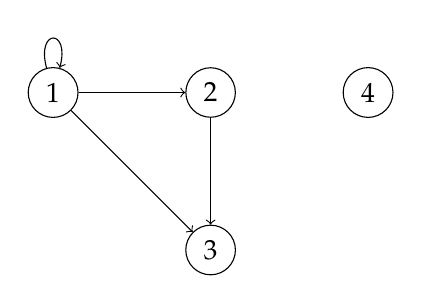
\begin{tikzpicture}[->,node distance=2cm]
  \node[draw,circle] (A) {$1$};
  \node[draw,circle] (B) [right of=A] {$2$};
  \node[draw,circle] (C) [below of=B] {$3$};
  \node[draw,circle] (D) [right of=B] {$4$};
  \draw (A) to [loop above]  (A);
  \draw (A) to  (B);
  \draw (A) to  (C);
  \draw (B) to  (C);
  \end{tikzpicture}
\intertext{Dit is niet dezelfde graaf als $\tuple{V', E}$ met $V' =
  \{1, 2, 3\}$. Die ziet er zo uit:}
& 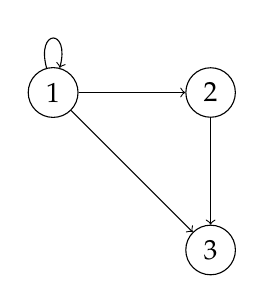
\begin{tikzpicture}[->,node distance=2cm]
  \node[draw,circle] (A) {$1$};
  \node[draw,circle] (B) [right of=A] {$2$};
  \node[draw,circle] (C) [below of=B] {$3$};
  \draw (A) to [loop above]  (A);
  \draw (A) to  (B);
  \draw (A) to  (C);
  \draw (B) to  (C);
  \end{tikzpicture}
\end{align*}
\end{ex}

\begin{prob}
  Zie de relatie ‘kleiner dan of gelijk aan’~$\le$ op de verzameling
  $\{1, 2, 3, 4\}$ als een graaf. Teken hoe die graaf eruitziet.
\end{prob}
% END ACCEPTED BODY OLP-0017
\endgroup
% END ACCEPTED UNIT OLP-0017

% BEGIN ACCEPTED UNIT OLP-0018 path=translations/nl-gewoon/content/sets-functions-relations/relations/trees.tex source-sha256=a43246ff47f14b1b4f3501c84b5d76c818f301c52b6b972a045a6869468a50ec
\begingroup
\def\olfilename{OLP-0018}
\def\olfilepath{content/sets-functions-relations/relations/}
\hypertarget{unit-OLP-0018}{}
\typeout{PARTIAL-READER-UNIT OLP-0018}
% BEGIN ACCEPTED BODY OLP-0018 body-sha256=fe2006994b6a67f27254037a517336c577c6e837bd1b714fd74d955c8fb85565
% Part: sets-functions-relations
% Chapter: relations
% Section: trees



\olfileid{sfr}{rel}{tre}
\olsection{Bomen}

Een \emph{boom} is een bepaald soort partiële ordening. Zulke bomen
spelen in elk deel van de logica een belangrijke rol. In de
eenvoudigere delen van de logica kom je eindige bomen tegen. Zo kun je
!!{formula}s begrijpen door te kijken hoe ze in een syntaxisboom in
kleinere delen uiteenvallen. Ook !!{derivation}s hebben in veel
systemen voor !!{derivation}s de vorm van een eindige boom.
%
Oneindige bomen kom je al tegen in het bewijs van de
volledigheidsstellingen voor propositielogica en eerste-ordelogica. Ze
worden in de hele wiskundige logica gebruikt.

Wat in de verzamelingenleer een boom heet, lijkt sterk op een boom uit
de grafentheorie. Zo ziet een (eindige) boom eruit:

\begin{center}
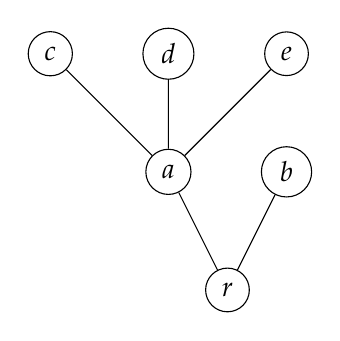
\begin{tikzpicture}[nodes={draw, circle}, -]
\node{$r$} [grow'=up]
    child { node {$a$} 
        child { node {$c$} }
        child { node {$d$} }
        child { node {$e$} }
    }
    child { node {$b$} };
\end{tikzpicture}
\end{center}

De onderste knoop~$r$ heet de wortel. Elke knoop behalve $r$ heeft
vlak eronder precies één ouder. Neem twee knopen~$x$ en~$y$. Kun je
$y$ vanuit~$x$ bereiken door de lijnen omhoog te volgen, dan heet $x$
een \emph{voorouder} van~$y$.

De voorouderrelatie van een boom is een strikte partiële ordening.
Daarom gebruiken we die relatie in de definitie met verzamelingen.
Eerst moeten we twee begrippen uitleggen. Een \emph{kleinste element}
in een verzameling~$A$ die partieel is geordend door~$\le$, is
!!a{element} $x \in A$ waarvoor bij elk $y \in A$ geldt dat~$x \le y$.
We noemen een verzameling door~$\le$ \emph{welgeordend} als elke
deelverzameling waar iets in zit een kleinste element heeft.

\begin{defn}[Boom]
Een \emph{boom} is een paar $T = \tuple{A, \le}$. Hier is $A$ een
verzameling en is $\le$ een partiële ordening op~$A$. Deze ordening
heeft precies één kleinste element $r \in A$ (de \emph{wortel}).
Verder is voor elk $x \in A$ de verzameling
$\Setabs{y}{y \le x}$ welgeordend door~$\le$.
\end{defn}

\begin{defn}[Opvolgers]
Neem een boom $T = \tuple{A, \le}$.
Als $x,y \in A$ en $x < y$, maar er geen $z \in A$ is met
$x < z < y$, dan heet $y$ een \emph{opvolger} van~$x$.
\end{defn}

De opvolgers van $x \in A$ heten ook zijn \emph{kinderen}. Is $y$ een
opvolger van~$x$, dan heet $x$ de \emph{voorganger} of \emph{ouder}
van~$y$.

\begin{prop}
Als $\tuple{A,\le}$ een boom is, kan elk $x \in A$ dat niet de wortel
is hoogstens één voorganger hebben.
\end{prop}

\begin{proof}
  Neem aan dat $y_1 < x$ en $y_2 < x$ en dat $y_1 \neq y_2$. Dan
  geldt $\{y_1, y_2\} \subseteq \Setabs{z}{z<x}$. De verzameling
  $\Setabs{z}{z<x}$ is welgeordend door~$\le$. Daarom heeft de
  deelverzameling $\{y_1, y_2\}$ een kleinste element. Dat moet $y_1$
  of~$y_2$ zijn. Dus $y_1 \le y_2$ of $y_2 \le y_1$. We hebben
  aangenomen dat $y_1 \neq y_2$, dus eigenlijk geldt $y_1 < y_2$ of
  $y_2 < y_1$. We weten ook dat $y_1 < x$ en $y_2 < x$. Daardoor
  geldt bovendien $y_1 < y_2 < x$ of $y_2 < y_1 < x$. De elementen
  $y_1$ en $y_2$ kunnen dus niet allebei voorgangers van~$x$ zijn.
\end{proof}

\begin{defn}
Een boom $T = \tuple{A, \le}$ noemen we \emph{oneindig} als $A$ een
oneindige verzameling is, en anders \emph{eindig}. Heeft $T$ de
eigenschap dat elke $x \in A$ maar eindig veel opvolgers heeft, dan
noemen we $T$ \emph{eindig vertakkend}.
\end{defn}

\begin{defn}[Takken]
Neem een boom $T = \tuple{A, \le}$. Een \emph{tak} van~$T$ is een
maximale keten in~$T$. Dat betekent hier dat $B \subseteq A$ en dat
voor elk tweetal $x, y \in B$ geldt dat $x \le y$ of $y \le x$.
Verder bestaat voor elke $z \in A \setminus B$ een $u \in B$ waarvoor
noch $z \le u$ noch $u \le z$ geldt.
%
We schrijven $[T]$ voor de verzameling van alle takken van $T$.
\end{defn}

\begin{ex}
Een bekend voorbeeld van een eindig vertakkende boom is de
\emph{oneindige binaire boom}. Die bestaat uit alle eindige rijen
van $0$'en en~$1$'en. We schrijven deze boom soms als $\{0,1\}^*$ of
als~$\Bin^*$. De uitbreidingsrelatie $\sqsubseteq$ bepaalt hun
volgorde. Zo geldt $101 \sqsubseteq 101101$: je krijgt de tweede rij
door achter de eerste nog cijfers te zetten. Achter elke binaire rij
kun je altijd een
$0$ of een $1$ zetten. Daarom heeft deze boom oneindig veel
elementen: bij elk element~$s$ horen precies twee opvolgers, $s0$
en~$s1$. De wortel is de lege rij $\emptyseq$.
\end{ex}

\begin{ex}
Iets algemener kun je eindige rijen van natuurlijke getallen nemen.
De verzameling daarvan,~$\Nat^*$, is met de
uitbreidingsrelatie~$\sqsubseteq$ ook een boom. Deze boom is duidelijk
niet eindig vertakkend: elke $s \in \Nat^*$ heeft oneindig veel
opvolgers~$sn$, één voor elke $n \in \Nat$. Elke
$A \subseteq \Nat^*$ die onder~$\sqsubseteq$ gesloten is, is een
\emph{deelboom} van~$\Nat^*$. (Dat betekent: $A$ is zo dat uit
$s \in A$ en $s' \sqsubseteq s$ ook $s' \in A$ volgt.) Elke eindige
boom kan worden voorgesteld als een eindige deelboom van~$\Nat^*$.
\end{ex}

\begin{prop}[Lemma van K\H{o}nig]
Als $T = \tuple{A,\le}$ een oneindige boom is die eindig vertakt, dan
heeft $T$ een oneindige tak.
\end{prop}

In de berekenbaarheidstheorie, de theorie van wat berekenbaar is, wordt
vaak een speciaal geval van het lemma van K\H{o}nig gebruikt. Het heet
het \emph{zwakke lemma van
K\H{o}nig} en zegt: elke oneindige deelboom van $\{0,1\}^*$ heeft een
oneindige tak.
% END ACCEPTED BODY OLP-0018
\endgroup
% END ACCEPTED UNIT OLP-0018

% BEGIN ACCEPTED UNIT OLP-0019 path=translations/nl-gewoon/content/sets-functions-relations/relations/operations.tex source-sha256=0c7e4f5e9b3e1a6c5dcd32ceaf7b2861a5065d4f0360bab6db552400e5881157
\begingroup
\def\olfilename{OLP-0019}
\def\olfilepath{content/sets-functions-relations/relations/}
\hypertarget{unit-OLP-0019}{}
\typeout{PARTIAL-READER-UNIT OLP-0019}
% BEGIN ACCEPTED BODY OLP-0019 body-sha256=06ebc05873cbfe0a70e15f99cc20cfd2eeb70d42b5465a719743f65598a96c54
% Part: sets-functions-relations
% Chapter: relations
% Section: operations



\olfileid{sfr}{rel}{ops}
\olsection{Wat je met relaties kunt doen}

Soms willen we relaties veranderen of met elkaar combineren. In
\olref[sfr][rel][ord]{prop:stricttopartial} hebben we relaties \emph{verenigd}.
Daarvoor bekijken we twee relaties als verzamelingen van paren en voegen we die
verzamelingen samen. In \olref[sfr][rel][ord]{prop:partialtostrict} hebben we
op dezelfde manier het relatieve verschil van relaties bekeken. Nu volgen
enkele andere dingen die we met relaties kunnen doen.

\begin{defn}\ollabel{relationoperations} 
Neem twee relaties $R$ en $S$, en een willekeurige verzameling $A$.

De \emph{inverse relatie} van $R$ is $R^{-1} = \Setabs{\tuple{y, x}}{\tuple{x,
    y} \in R}$. Daarin is elk paar omgedraaid.

De \emph{samenstelling} van $R$ en $S$ is $(R \mid S) =
\{\tuple{x, z} : \exists y(Rxy \land Syz)\}$. Je gaat dus eerst via de
eerste relatie naar een element in het midden en daarna via de tweede relatie
naar het laatste element.

De \emph{restrictie} van $R$ tot $A$ is $\funrestrictionto{R}{A}= R
\cap A^2$. Je houdt daarmee alleen de paren uit die relatie over waarvan
beide delen in de opgegeven verzameling liggen.

Het door $R$ bepaalde \emph{beeld} van $A$ is $\funimage{R}{A} = \{y :
(\exists x \in A)Rxy\}$. Dit is de verzameling van alle tweede elementen die
via de relatie bij minstens één element uit de opgegeven verzameling horen.
\end{defn}

\begin{ex}
Neem de opvolgerrelatie $S \subseteq \Int^2$ op~$\Int$. Dat wil zeggen:
$S = \Setabs{\tuple{x, y} \in \Int^2}{x + 1 = y}$. Dus $Sxy$ geldt precies
als $x + 1 = y$.

$S^{-1}$ is de voorgangerrelatie op $\Int$, dus
$\Setabs{\tuple{x,y}\in\Int^2}{x -1 =y}$.

$S\mid S$ is
$ \Setabs{\tuple{x,y}\in\Int^2}{x + 2 =y}$

$\funrestrictionto{S}{\Nat}$ is de opvolgerrelatie op~$\Nat$.

$\funimage{S}{\{1,2,3\}}$ is $\{2, 3, 4\}$.
\end{ex}

\begin{defn}[Transitieve afsluiting]Neem een binaire relatie $R \subseteq A^2$.
	
De \emph{transitieve afsluiting} van~$R$ is $R^+ = \bigcup_{0 < n \in
\Nat} R^n$. De machten bouwen we stap voor stap op: $R^1 = R$ en
$R^{n+1} = R^n \mid R$.

De \emph{reflexief-transitieve afsluiting} van $R$ is $R^* = R^+ \cup
\Id{A}$. Daarmee voeg je ook alle paren toe van elementen uit de opgegeven
verzameling waarin het eerste en het tweede element hetzelfde zijn.
\end{defn}

\begin{ex}
Neem de opvolgerrelatie $S \subseteq \Int^2$. $S^2xy$ geldt precies als
$x + 2 = y$, $S^3xy$ precies als $x + 3 = y$, enzovoort. $S^+xy$ geldt dus
precies als $x + n = y$ voor een bepaalde $n \geq 1$. Of korter: $S^+xy$
geldt precies als $x < y$, en $S^*xy$ precies als $x \le y$.
\end{ex}

\begin{prob}
Laat zien dat de transitieve afsluiting van $R$ inderdaad transitief is.
\end{prob}
% END ACCEPTED BODY OLP-0019
\endgroup
% END ACCEPTED UNIT OLP-0019
\OLEndChapterHook

% BEGIN ACCEPTED UNIT OLP-0020 path=translations/nl-gewoon/content/sets-functions-relations/functions/functions.tex source-sha256=095199b52971703373d2cd9bfd0103450e30a405145e63084981deba8bef1a60
\begingroup
\def\olfilename{OLP-0020}
\def\olfilepath{content/sets-functions-relations/functions/}
\hypertarget{unit-OLP-0020}{}
\typeout{PARTIAL-READER-UNIT OLP-0020}
% BEGIN ACCEPTED BODY OLP-0020 body-sha256=aac34667a2f86c82d6ddb67aeb2ecfd3f72f23f3edf8551699815f2d9c30070a
% Part: sets-functions-relations
% Chapter: functions



\olchapter{sfr}{fun}{Functies}
% END ACCEPTED BODY OLP-0020
\endgroup
% END ACCEPTED UNIT OLP-0020

% BEGIN ACCEPTED UNIT OLP-0021 path=translations/nl-gewoon/content/sets-functions-relations/functions/function-basics.tex source-sha256=993613ab3815794f31147d43304056f3411823dcd0ee037fea0676ecd422fac4
\begingroup
\def\olfilename{OLP-0021}
\def\olfilepath{content/sets-functions-relations/functions/}
\hypertarget{unit-OLP-0021}{}
\typeout{PARTIAL-READER-UNIT OLP-0021}
% BEGIN ACCEPTED BODY OLP-0021 body-sha256=4c1a4267841da847737b213be469f7c86eee5242470a52f84f9042781820a634
% Part: sets-functions-relations
% Chapter: functions
% Section: basics



\olfileid{sfr}{fun}{bas}
\olsection{De basis}

\begin{explain}
Een \emph{functie} koppelt elk !!{element} uit een bepaalde verzameling aan
één bepaald !!{element} uit een andere verzameling, of soms uit dezelfde.
Optellen met~$1$ geeft bijvoorbeeld een functie: bij elk getal~$n$ hoort
precies één getal~$n+1$.
  
De invoer van een functie kan ook een paar, een drietal of iets met nog meer
delen zijn. Daar geeft de functie dan een uitvoer bij. Veel functies kennen we
al van gewoon rekenen.
Optellen en vermenigvuldigen zijn er voorbeelden van: je voert twee getallen
in en krijgt één getal als uitkomst.

Als wiskundig, abstract begrip is een functie een \emph{zwarte doos}. Het gaat
er alleen om welke uitvoer bij welke invoer hoort. Hoe je die uitvoer berekent,
doet er niet toe.
\end{explain}

\begin{defn}[Functie]
Een \emph{functie} $f \colon A \to B$ koppelt elk !!{element} van~$A$ aan
precies één !!{element} van~$B$.

$A$ heet het \emph{domein} van~$f$: daar komen de invoeren vandaan. $B$ heet
het \emph{codomein} van~$f$: daarin liggen de mogelijke uitkomsten. De
!!{element}en van~$A$ heten invoeren of \emph{argumenten}
van~$f$. Het !!{element} van~$B$ dat bij een argument~$x$ hoort volgens~$f$,
heet de \emph{waarde van~$f$} bij argument~$x$. We schrijven die als~$f(x)$.

Het \emph{bereik} $\ran{f}$ van~$f$ is het deel van het codomein waarin de
waarden van~$f$ staan die bij minstens één argument horen; $\ran{f} =
\Setabs{f(x)}{x \in A}$.
\end{defn}

Het plaatje in \olref{fig:function} kan helpen. De ellips links is het
\emph{domein} van de functie en de ellips rechts is het \emph{codomein}.
Een pijl gaat van een \emph{argument} in het domein naar de \emph{waarde} die
er in het codomein bij hoort.

\begin{figure}
  \olasset{assets/diagrams/function.tikz}
  \caption{Een functie koppelt elk !!{element} van de ene verzameling aan
    !!a{element} van een andere. Een pijl gaat van een argument in het
    domein naar de waarde die er in het codomein bij hoort.}
  \ollabel{fig:function}
\end{figure}

\begin{ex}
Bij vermenigvuldigen voer je twee natuurlijke getallen in en krijg je een
natuurlijk getal terug. Dit is dus een functie van $\Nat \times \Nat$ (het
domein) naar $\Nat$ (het codomein). Het bereik is ook $\Nat$, want elke
$n \in \Nat$ is gelijk aan $n \times 1$.
\end{ex}

\begin{ex}
Vermenigvuldigen is een functie: bij elke invoer---elk paar natuurlijke
getallen---hoort maar één uitvoer: $\times \colon \Nat^2 \to
\Nat$. Koppel je een natuurlijk getal~$n$ aan een reëel getal~$x$ waarvoor
$x^2 = n$, dan krijg je geen functie. Elk positief geheel getal~$n$ heeft
namelijk twee vierkantswortels: $\sqrt{n}$ en~$-\sqrt{n}$. We kunnen er een
functie van maken door alleen de niet-negatieve vierkantswortel terug te geven:
$\sqrt{\phantom{X}} \colon \Nat \to \Real$.
\end{ex}

\begin{ex}
Koppel je elke leerling in een klas aan het eindcijfer dat die leerling in die
klas krijgt, dan krijg je een functie. Een leerling kan binnen dezelfde klas
geen twee verschillende eindcijfers krijgen. Koppel je elke leerling aan de
ouders van die leerling, dan krijg je geen functie: een leerling kan nul, twee
of meer ouders hebben.
\end{ex}

\begin{explain}
Om precies te zeggen welke functie we bedoelen, moeten we voor elke mogelijke
invoer aangeven welke waarde erbij hoort. Dat kan met een formule, met een
manier om de waarde uit te rekenen of met een lijst waarin voor elke invoer de
waarde staat.
Welke manier we ook kiezen, bij elke invoer moet één, en maar één, waarde staan.
\end{explain}


\begin{ex}
Definieer $f \colon \Nat \to \Nat$ met $f(x) = x+1$. Daarmee hebben we een
functie $f$ die natuurlijke getallen binnenkrijgt en natuurlijke getallen
teruggeeft. Voer je een natuurlijk getal~$x$ in, dan geeft $f$ de opvolger,
het volgende getal~$x+1$. Het codomein $\Nat$ is hier niet het bereik van~$f$:
het natuurlijke getal~$0$ komt nooit uit deze functie, want het volgt op geen enkel
natuurlijk getal. Het bereik van~$f$ bestaat uit alle positieve gehele
getallen, $\Int^{+}$.
\end{ex}

\begin{ex}\ollabel{examplefunext}
Definieer $g \colon \Nat \to \Nat$ met $g(x) = x+2-1$. Dit is een functie
$g$ die natuurlijke getallen binnenkrijgt en natuurlijke getallen teruggeeft.
Bij een natuurlijk getal~$x$ geeft $g$ de uitkomst die je krijgt door vanaf
$x$ twee stappen vooruit en één stap terug te gaan, dus $x+1$.
\end{ex}

\begin{explain}
We hebben nu twee functies, $f$ en $g$, met verschillende \emph{definities}.
Toch zijn het \emph{dezelfde functie}. Voor elk natuurlijk getal~$n$ geldt
namelijk $f(n) = n+1 = n+2-1 = g(n)$. Anders gezegd: de definities van $f$
en~$g$ gebruiken verschillende vergelijkingen, maar leggen dezelfde koppeling
vast. Daarachter zit het extensionaliteitsbeginsel voor functies: twee functies
zijn gelijk als ze bij elke invoer dezelfde waarde geven. In symbolen:
\[
  \text{als }\forall x\, f(x) = g(x)\text{, dan }f = g
\]
Dit geldt alleen als $f$ en~$g$ hetzelfde domein én hetzelfde codomein hebben.
\end{explain}

\begin{ex}
We kunnen een functie ook geval voor geval beschrijven: per geval geven we aan
welke regel geldt. Zo kunnen we $h \colon \Nat \to \Nat$ definiëren:
\[
h(x) =
\begin{cases}
  \frac{x}{2} & \text{als $x$ even is} \\
  \frac{x+1}{2} & \text{als $x$ oneven is.}
\end{cases}
\]
Elk natuurlijk getal is even of oneven, dus de uitvoer van deze functie is
altijd een natuurlijk getal. Let er bij zo'n beschrijving op dat elke mogelijke
invoer in precies één geval valt. Soms moet je bewijzen dat elke mogelijke
invoer in een van de gevallen valt en nooit in twee gevallen tegelijk.
\end{ex}
% END ACCEPTED BODY OLP-0021
\endgroup
% END ACCEPTED UNIT OLP-0021

% BEGIN ACCEPTED UNIT OLP-0022 path=translations/nl-gewoon/content/sets-functions-relations/functions/function-kinds.tex source-sha256=3f656abb22dc9510bcc14d4af37cae2d3d906ffc5abd77feb2f7023ec61b75e1
\begingroup
\def\olfilename{OLP-0022}
\def\olfilepath{content/sets-functions-relations/functions/}
\hypertarget{unit-OLP-0022}{}
\typeout{PARTIAL-READER-UNIT OLP-0022}
% BEGIN ACCEPTED BODY OLP-0022 body-sha256=7f9177105655f4604b85ec37ec93cc4cf990c7f43d183869208ede6d5d96cc29
% Part: sets-functions-relations
% Chapter: functions
% Section: kinds



\olfileid{sfr}{fun}{kin}
\olsection{Verschillende soorten functies}

\begin{explain}
Het helpt om de soorten functies die we vaak tegenkomen in groepen in
te delen.

We beginnen met functies waarbij ieder element van het codomein ook
echt als waarde voorkomt. Zo'n functie heet !!{surjective}. De
afbeelding in \olref{fig:surjective} laat dit zien.

\begin{figure}
  \olasset{assets/diagrams/surjective.tikz}
  \caption{Bij !!^a{surjective} functie komt ieder !!{element} van het
    codomein als waarde voor.}
  \ollabel{fig:surjective}
\end{figure}
\end{explain}

\begin{defn}[!!^{surjective} functie]
Een functie $f \colon A \rightarrow B$ heet \emph{!!{surjective}}
precies wanneer $B$ ook het bereik van~$f$ is. Dat betekent: voor elke
$y \in B$ is er minstens één $x \in A$ waarvoor~$f(x) = y$, of in
symbolen:
\[
  (\forall y \in B)(\exists x \in A)f(x) = y.
\]
Zo'n functie noemen we !!a{surjection} van $A$ naar $B$.
\end{defn}

\begin{explain}
Wil je laten zien dat $f$ !!a{surjection} is, dan moet je laten zien
dat ieder object in het codomein van $f$ de waarde $f(x)$ is bij een
invoer $x$.

Elke functie \emph{levert} !!a{surjection} op. Neem namelijk een
functie $f \colon A \to B$ en maak $f' \colon A \to \ran{f}$ met
$f'(x) = f(x)$. Het bereik $\ran{f}$ is \emph{per definitie}
$\Setabs{f(x) \in B}{x \in A}$. Daarom is deze functie $f'$ zeker
!!a{surjection}.
\end{explain}

\begin{explain}
Elke mogelijke invoer van een functie krijgt precies één uitvoer. Bij
sommige functies krijgen twee verschillende invoeren bovendien nooit
dezelfde uitvoer. Zo'n functie heet !!{injective}. De afbeelding in
\olref{fig:injective} laat dit zien.
\begin{figure}
  \olasset{assets/diagrams/injective.tikz}
  \caption{!!^a{injective} functie geeft nooit dezelfde waarde aan
    twee verschillende argumenten.}
  \ollabel{fig:injective}
\end{figure}
\end{explain}

\begin{defn}[!!^{injective} functie]
Een functie $f \colon A \rightarrow B$ heet \emph{!!{injective}}
precies wanneer er bij elke $y \in B$ hoogstens één $x \in A$ is
waarvoor~$f(x) = y$. Zo'n functie noemen we !!a{injection} van $A$
naar~$B$.
\end{defn}

\begin{explain}
Wil je laten zien dat $f$ !!a{injection} is, neem dan willekeurige
!!{element}s $x$ en $y$ uit het domein van $f$. Je moet bewijzen: als
$f(x)=f(y)$, dan $x=y$.
\end{explain}

\begin{ex}
De constante functie $f\colon \Nat \to \Nat$ met $f(x) = 1$ is niet
!!{injective} en ook niet !!{surjective}.

De identiteitsfunctie $f\colon \Nat \to \Nat$ met $f(x) = x$ is
!!{injective} én !!{surjective}.

De opvolgerfunctie $f \colon \Nat \to \Nat$ met $f(x) = x+1$ is
!!{injective}, maar niet !!{surjective}.
  
De functie $f \colon \Nat \to \Nat$ die als volgt is vastgelegd,
\[
  f(x) =
  \begin{cases}
    \frac{x}{2} & \text{als $x$ even is} \\
    \frac{x+1}{2} & \text{als $x$ oneven is.}
  \end{cases}
\]
is !!{surjective}, maar niet !!{injective}.
\end{ex}

\begin{explain}
Vaak hebben we een functie nodig die tegelijk !!{injective} en
!!{surjective} is. Zo'n functie heet !!{bijective}. Zij ziet eruit als
de functie in \olref{fig:bijective}. !!^{bijection}s heten ook wel
\emph{een-op-een-koppelingen}: ze koppelen ieder element van het
codomein aan precies één element van het domein.
\begin{figure}
  \olasset{assets/diagrams/bijective.tikz}
  \caption{!!^a{bijective} functie koppelt ieder element van het
    codomein aan precies één element van het domein.}
  \ollabel{fig:bijective}
\end{figure}
\end{explain}

\begin{defn}[!!^{bijection}]
Een functie $f \colon A \to B$ heet \emph{!!{bijective}} precies
wanneer zij zowel !!{surjective} als !!{injective} is. Zo'n functie
noemen we !!a{bijection} van $A$ naar~$B$ (of tussen $A$ en~$B$).
\end{defn}
% END ACCEPTED BODY OLP-0022
\endgroup
% END ACCEPTED UNIT OLP-0022

% BEGIN ACCEPTED UNIT OLP-0023 path=translations/nl-gewoon/content/sets-functions-relations/functions/functions-relations.tex source-sha256=e02bcb72366c8b12d063f3cd9dd4f642f884b2b5bbf157971cdf8f376f73e135
\begingroup
\def\olfilename{OLP-0023}
\def\olfilepath{content/sets-functions-relations/functions/}
\hypertarget{unit-OLP-0023}{}
\typeout{PARTIAL-READER-UNIT OLP-0023}
% BEGIN ACCEPTED BODY OLP-0023 body-sha256=d2f9d34ef252f9b0c34d1f2ffc8b66adabf4535e7f2d002f92605a8273c11c75
% Part: sets-functions-relations
% Chapter: functions
% Section: functions-relations




\olfileid{sfr}{fun}{rel}

\olsection{Functies als relaties}

\begin{explain}
Een functie die !!{element}s van~$A$ naar !!{element}s van~$B$ stuurt,
legt meteen een relatie tussen $A$ en~$B$ vast. Die relatie geldt voor
$x$ en $y$ precies wanneer $f(x) = y$. Soms willen we de wiskunde met
zo weinig mogelijk bouwstenen opbouwen. Dan kunnen we de functie~$f$
\emph{zien als} deze relatie, dus als een verzameling paren. De vraag
is dan: welke relaties leggen op deze manier een functie vast?
\end{explain}

\begin{defn}[Grafiek van een functie] Neem een functie $f\colon A \to
B$. De \emph{grafiek} van~$f$ is de relatie $R_f \subseteq A \times
B$ die als volgt is vastgelegd:
\[
R_f = \Setabs{\tuple{x,y}}{f(x) = y}.
\]
\end{defn}

\begin{explain}
Door extensionaliteit ligt de grafiek van een functie helemaal vast.
Dezelfde regel geeft ook de stilzwijgende regel van extensionaliteit
voor functies: hebben $f$ en~$g$ hetzelfde domein en codomein, dan
zijn ze gelijk als ze bij elke invoer dezelfde waarde geven.

Net zo geldt: is een relatie ‘functioneel’, dan is zij de grafiek van
een functie.
\end{explain}

\begin{prop}\ollabel{prop:graph-function}
Neem $R \subseteq A \times B$ waarvoor de volgende twee dingen gelden:
\begin{enumerate}
\item Als $Rxy$ en $Rxz$, dan $y = z$; en
\item bij elke $x \in A$ is er een $y \in B$ waarvoor $\tuple{x,
y} \in R$.
\end{enumerate}
Dan is $R$ de grafiek van de functie $f\colon A \to B$ die is
vastgelegd door $f(x) = y$ precies wanneer $Rxy$.
\end{prop}

\begin{proof}
Neem aan dat er een $y$ is waarvoor $Rxy$ geldt. Als er ook een $z
\neq y$ was waarvoor $Rxz$ geldt, zou $R$ niet aan de voorwaarde
voldoen. Als er een $y$ is waarvoor $Rxy$ geldt, is deze $y$ dus de
enige. Daarom is $f$ goed vastgelegd. Het is duidelijk dat $R_f = R$.
\end{proof}

\begin{explain}
Elke functie $f\colon A \to B$ heeft een grafiek: een relatie die uit
paren in $A \times B$ bestaat en is vastgelegd door $f(x) = y$.
Omgekeerd is elke
relatie~$R \subseteq A \times B$ met de eigenschappen uit
\olref{prop:graph-function} de grafiek van een functie~$f \colon A \to
B$. Door dit nauwe verband kunnen we een functie gewoon als haar
grafiek zien. Met andere woorden: we kunnen functies zien als bepaalde
relaties, dus als bepaalde verzamelingen tupels.
\oliflabeldef{sfr:rel:ref:sec}{Let wel: met deze ‘identificatie’
bedoelen we hetzelfde als in \olref[sfr][rel][ref]{sec}. We doen geen
uitspraak over wat functies in diepste zin zijn; we merken alleen op
dat het handig is om functies als bepaalde verzamelingen te
\emph{zien}. Dat heeft dit voordeel: w}{W}e kunnen nu op functies
dezelfde soort bewerkingen uitvoeren als eerder op relaties (zie
\olref[sfr][rel][ops]{sec}). In het bijzonder:
\end{explain}

\begin{defn}\ollabel{defn:funimage}
Neem een functie $f \colon A \to B$ met $C\subseteq A$.

De \emph{beperking} van~$f$ tot~$C$ is de
functie~$\funrestrictionto{f}{C}\colon C \to B$ waarvoor
$(\funrestrictionto{f}{C})(x) = f(x)$ voor alle $x \in C$. Anders
gezegd: $\funrestrictionto{f}{C} = \Setabs{\tuple{x, y} \in R_f}{x
\in C}$.

Als we~$f$ op~$C$ \emph{toepassen}, krijgen we $\funimage{f}{C} =
\Setabs{f(x)}{x \in C}$. We noemen dit ook het \emph{beeld} van~$C$
onder~$f$.
\end{defn}

\begin{explain}
Uit deze definities volgt dat $\ran{f} =
\funimage{f}{\dom{f}}$ voor elke functie~$f$.
\oliflabeldef{sfr:rel:ops:sec}{Deze begrippen werken precies zoals je
zou verwachten uit de definities in
\olref[sfr][rel][ops]{sec} en uit het feit dat we functies als relaties
zien. Twee andere bewerkingen hebben wat meer uitleg nodig: inversen nemen en
relaties samenstellen. Die geven we in
\olref[inv]{sec} en \olref[cmp]{sec}.}{}
\end{explain}
% END ACCEPTED BODY OLP-0023
\endgroup
% END ACCEPTED UNIT OLP-0023

% BEGIN ACCEPTED UNIT OLP-0024 path=translations/nl-gewoon/content/sets-functions-relations/functions/inverses.tex source-sha256=0911403bee44a1f70aa91b4ecb739cd67273f3f43ddf95eb7e097f3d41fe80c7
\begingroup
\def\olfilename{OLP-0024}
\def\olfilepath{content/sets-functions-relations/functions/}
\hypertarget{unit-OLP-0024}{}
\typeout{PARTIAL-READER-UNIT OLP-0024}
% BEGIN ACCEPTED BODY OLP-0024 body-sha256=b87b746cf94ccffe137c58b156af9922726c5114c35fcc3bbaa6e44c69eb6566
% Part: sets-functions-relations
% Chapter: functions
% Section: inverses



\olfileid{sfr}{fun}{inv}
\olsection{Functies omkeren}

\begin{explain}
Je kunt een functie zien als iets dat een invoer naar een uitvoer
stuurt. Dan ligt één vraag voor de hand: kan dat ook ``omgekeerd''?
Bijvoorbeeld: de opvolgerfunctie $f(x) = x + 1$ kun je omkeren. De
functie $g(y) = y - 1$ maakt dan ``ongedaan'' wat $f$ doet.

Maar je moet wel opletten. De definitie van~$g$ geeft een functie
$\Int \to \Int$, maar geen \emph{functie} $\Nat \to \Nat$, want
$g(0) \notin \Nat$. Zelfs bij zo'n eenvoudig voorbeeld is dus niet
meteen duidelijk of je een functie kunt omkeren. Dat kan afhangen van
het domein en codomein: van de verzameling waaruit de invoer komt en de
verzameling waarin de uitvoer moet liggen.

Daarvoor gebruiken we het begrip inverse van een functie.
\end{explain}

\begin{defn}
Een functie $g \colon B \to A$ is een \emph{inverse} van een functie
$f \colon A \to B$ als $f(g(y)) = y$ en $g(f(x)) = x$ voor alle $x
\in A$ en $y \in B$.
\end{defn}

Als $f$ een inverse~$g$ heeft, schrijven we vaak $f^{-1}$ in plaats
van~$g$.

\begin{explain}
Nu zoeken we uit wanneer een functie een inverse heeft. Voor
$f\colon A \to B$ lijkt $g\colon B \to A$ een goede keuze. We zouden
deze functie als volgt willen ``definiëren'':
\[
g(y) = \text{``de'' $x$ waarvoor $f(x) = y$.}
\]
De aanhalingstekens rond ``definiëren'' (en rond ``de'') verraden al
dat dit nog geen echte definitie is. Dit werkt namelijk niet altijd.
Om hiermee een functie te bepalen, moet er precies één~$x$ zijn
waarvoor $f(x) = y$. De uitvoer van~$g$ moet maar op één manier zijn
vastgelegd. Ook moet er voor elke $y \in B$ een uitvoer zijn. Als er
$x_1$ en $x_2 \in A$ zijn met $x_1 \neq x_2$ maar $f(x_1) = f(x_2)$,
dan heeft $g(y)$ geen unieke waarde voor $y = f(x_1) = f(x_2)$. En als
er helemaal geen~$x$ is waarvoor $f(x) = y$, dan is $g(y)$ helemaal
niet vastgelegd. Kortom, $g$ is alleen zo te definiëren als $f$ zowel
!!{injective} is (verschillende invoeren krijgen verschillende
uitvoeren) als !!{surjective} (elke mogelijke uitvoer wordt bereikt).

We nemen dit stap voor stap en splitsen de vraag in twee delen. Neem
een functie~$f\colon A \to B$. Wanneer bestaat er een functie
$g\colon B \to A$ waarvoor $g(f(x)) = x$? Zo'n $g$ ``maakt ongedaan''
wat $f$ doet en heet een \emph{linksinverse} van~$f$. En wanneer bestaat
er een functie $h\colon B \to A$ waarvoor $f(h(y)) = y$? Zo'n $h$
heet een \emph{rechtsinverse} van~$f$: $f$ ``maakt ongedaan'' wat
$h$~doet.
\end{explain}

\begin{prop}
Als het domein niet leeg is en $f\colon A \to B$ !!{injective} is, dan
bestaat er een
\emph{linksinverse}~$g\colon B \to A$ van~$f$ waarvoor $g(f(x)) = x$
voor alle $x \in A$.
\end{prop}

\begin{proof}
Stel dat het domein niet leeg is en dat $f\colon A \to B$
!!{injective} is. Neem een $y \in B$. Als
$y \in \ran{f}$, dan is er een $x \in A$ waarvoor $f(x) = y$. Omdat
$f$ !!{injective} is, is er maar één zo'n~$x \in A$. We kunnen dus
$g(y) = x$ nemen. Anders gezegd: $g(y)$ is ``de'' $x \in A$ waarvoor
$f(x) = y$. Als $y \notin \ran{f}$, mogen we die naar elk
willekeurig~$a \in A$ sturen. We kiezen daarom een $a \in A$ en leggen
$g\colon B \to A$ zo vast:
\[
g(y) = \begin{cases}
    x & \text{als $f(x) = y$}\\
    a & \text{als $y \notin \ran{f}$.}
\end{cases}
\]
De functie is nu voor elke $y \in B$ vastgelegd: als zo'n $y \in \ran{f}$
ligt, is er precies één $x \in A$ waarvoor $f(x) = y$. Uit de
definitie volgt dat als $y = f(x)$, dan $g(y) = x$, en dus
$g(f(x)) = x$.
\end{proof}

\begin{prob}
Laat zien dat als $f\colon A \to B$ een linksinverse~$g$ heeft,
$f$~!!{injective} is.
\end{prob}

\begin{prop}
    Als $f\colon A \to B$ !!{surjective} is, dan bestaat er een
    \emph{rechtsinverse}~$h\colon B \to A$ van~$f$ waarvoor $f(h(y)) =
    y$ voor alle~$y \in B$.
\end{prop}

\begin{proof}
Stel dat $f\colon A \to B$ !!{surjective} is. Neem een $y \in B$.
Omdat $f$~!!{surjective} is, is er een $x_y \in A$ met $f(x_y) = y$.
We kunnen dus $h(y) = x_y$ nemen. Dat betekent: voor elke $y \in B$
kiezen we een $x \in A$ waarvoor $f(x) = y$. Omdat $f$~!!{surjective}
is, valt er altijd minstens één te kiezen.\footnote{Omdat $f$
!!{surjective} is, is voor elke~$y \in B$ de verzameling
$\Setabs{x}{f(x) = y}$ niet leeg. Voor onze definitie van~$h$ moeten
we uit elk van deze verzamelingen één $x$ kiezen. Het spreekt niet
vanzelf dat dit altijd kan. We nemen die mogelijkheid gewoon als een
axioma aan. Anders gezegd: deze stelling gebruikt het zogeheten
keuzeaxioma. Dit is een punt waarop we
\oliflabeldef{sth:choice::chap}{terugkomen in \olref[sth][choice][]{chap}}{hier niet verder ingaan}.
Maar in veel concrete gevallen is het keuzeaxioma niet nodig,
bijvoorbeeld als $A = \Nat$ of eindig is, of als $f$ !!{bijective} is.
(Als $f$ !!{bijective} is, heeft voor elke $y \in B$ de verzameling
$\Setabs{x}{f(x) = y}$ precies één !!{element}.
Er valt dan dus niets te kiezen.)}
Volgens de definitie geldt: als $x = h(y)$, dan $f(x) = y$. Dus voor
elke $y \in B$ geldt $f(h(y)) = y$.
\end{proof}

\begin{prob}
Laat zien dat als $f\colon A \to B$ een rechtsinverse~$h$ heeft,
$f$~!!{surjective} is.
\end{prob}

\begin{explain}
  Als we de ideeën uit het vorige bewijs samenvoegen, zien we dat elke
  !!{bijection} een inverse heeft. Er is dus één functie die tegelijk
  linksinverse en rechtsinverse van~$f$ is.
\end{explain}

\begin{prop}\ollabel{prop:bijection-inverse}
Als $f\colon A \to B$ !!{bijective} is, dan bestaat er een
functie~$f^{-1}\colon B \to A$ waarvoor voor alle $x \in A$ geldt:
$f^{-1}(f(x)) = x$, en voor alle $y \in B$: $f(f^{-1}(y)) = y$.
\end{prop}

\begin{proof}
Oefening.
\end{proof}

\begin{prob}
Bewijs \olref[sfr][fun][inv]{prop:bijection-inverse}. Je moet~$f^{-1}$
definiëren, laten zien dat dit een functie is en laten zien
dat het een inverse van~$f$ is. Dus: $f^{-1}(f(x)) = x$ en
$f(f^{-1}(y)) = y$ voor alle $x \in A$ en $y \in B$.
\end{prob}

\begin{explain}
Je kunt ook in iets meer gevallen aan een inverse komen. In
\olref[kin]{sec} zagen we dat elke functie $f$ een !!a{surjection} $f'
\colon A \to \ran{f}$ oplevert door $f'(x) = f(x)$ te nemen voor alle
$x \in A$. Als $f$~!!{injective} is, dan is $f'$~!!{bijective}.
Volgens \olref{prop:bijection-inverse} heeft deze functie dus een
unieke inverse. We zijn dan een klein beetje slordig met de notatie en
noemen de inverse van $f'$ soms gewoon ``de inverse van~$f$.''
\end{explain}

\begin{prop}\ollabel{prop:left-right}%
  Laat zien dat als $f\colon A \to B$ een linksinverse~$g$ en een
  rechtsinverse~$h$ heeft, dan $h = g$.
\end{prop}

\begin{proof}
  Oefening.
\end{proof}

\begin{prob}
  Bewijs \olref[sfr][fun][inv]{prop:left-right}.
\end{prob}

\begin{prop}\ollabel{prop:inverse-unique}
Een functie~$f$ kan nooit meer dan één inverse hebben.
\end{prop}

\begin{proof}
  Stel dat $g$ en $h$ allebei inversen van~$f$ zijn. Dan is $g$ in elk
  geval een linksinverse van~$f$ en is $h$ een rechtsinverse. Uit
  \olref{prop:left-right} volgt $g = h$.
\end{proof}
% END ACCEPTED BODY OLP-0024
\endgroup
% END ACCEPTED UNIT OLP-0024

% BEGIN ACCEPTED UNIT OLP-0025 path=translations/nl-gewoon/content/sets-functions-relations/functions/composition.tex source-sha256=e55828b6ba92b3f73002cbe9932faca7d613fe944a11d2f9742ba1f434808820
\begingroup
\def\olfilename{OLP-0025}
\def\olfilepath{content/sets-functions-relations/functions/}
\hypertarget{unit-OLP-0025}{}
\typeout{PARTIAL-READER-UNIT OLP-0025}
% BEGIN ACCEPTED BODY OLP-0025 body-sha256=65366c306c0347ce6dba83fa62059cec11859fad39542673f6e20def840cdeb2
% Part: sets-functions-relations
% Chapter: functions
% Section: composition



\olfileid{sfr}{fun}{cmp}
\olsection{Samenstelling: functies na elkaar gebruiken}

\begin{explain}
\oliflabeldef{sfr:fun:inv:sec}{In \olref[inv]{sec} zagen we dat de
inverse~$f^{-1}$ van !!a{bijection}~$f$ zelf ook een functie is. Nog
een manier om functies te gebruiken is ze samen te stellen: w}{W}e
kunnen uit twee functies, $f$ en~$g$, één nieuwe functie maken. We
gebruiken eerst $f$ en daarna~$g$. Dat werkt alleen wanneer alle
uitkomsten van de eerste functie geldige invoeren voor de tweede zijn.
Anders gezegd: het beeld van~$f$ moet een deelverzameling zijn van het
domein van~$g$.
\oliflabeldef{sfr:rel:ops:sec}{Functies op deze manier samenstellen is
vergelijkbaar met relaties samenstellen zoals beschreven in
\olref[rel][ops]{sec}.}{}

Een plaatje kan duidelijk maken wat er gebeurt. In
\olref{fig:composition} staan twee functies, $f \colon A \to B$ en
$g \colon B \to C$, en hun samenstelling~$(\comp{f}{g})$. De functie
$(\comp{f}{g}) \colon A \to C$ koppelt elk !!{element} van~$A$ aan
!!a{element} van~$C$. Zo bepalen we welk !!{element} van~$C$ bij
!!a{element} van $A$ hoort. Neem een invoer $x \in A$. Gebruik eerst
de functie $f$ voor~$x$; de uitkomst is $f(x) = y \in B$. Gebruik
daarna de functie $g$ voor~$y$; de uitkomst is $g(f(x)) = g(y) = z
\in C$.
\begin{figure}
  \olasset[2\olphotowidth]{assets/diagrams/composition.tikz}
  \caption{De samenstelling $g \circ f$: eerst $f$ en daarna~$g$.}
  \ollabel{fig:composition}
\end{figure}
\end{explain}

\begin{defn}[Samenstelling]
Neem de functies $f\colon A \to B$ en $g\colon B \to C$. De
\emph{samenstelling} van $f$ met~$g$ is $\comp{f}{g} \colon A \to C$.
Voor elke invoer geldt $(\comp{f}{g})(x) = g(f(x))$.
\end{defn}

\begin{ex}
Neem de functies $f(x) = x + 1$ en $g(x) = 2x$. Omdat
$(\comp{f}{g})(x) = g(f(x))$, tel je bij elke invoer~$x$ eerst één op.
Daarna verdubbel je de uitkomst. De samenstelling is dus
$(\comp{f}{g})(x) = 2(x+1)$.
\end{ex}

\begin{prob}
Bewijs dat als $f \colon A \to B$ en $g \colon B \to C$ allebei
!!{injective} zijn---verschillende invoeren geven dus verschillende
uitkomsten---ook $\comp{f}{g}\colon A \to C$ !!{injective} is.
\end{prob}

\begin{prob}
Bewijs dat als $f \colon A \to B$ en $g \colon B \to C$ allebei
!!{surjective} zijn---ze bereiken dus elk element van hun
doelverzameling---ook $\comp{f}{g}\colon A \to C$ !!{surjective} is.
\end{prob}

\begin{prob}
Neem $f \colon A \to B$ en $g \colon B \to C$. De grafiek van
$\comp{f}{g}$ moet $R_f \mid R_g$ zijn. Laat dat zien.
\end{prob}
% END ACCEPTED BODY OLP-0025
\endgroup
% END ACCEPTED UNIT OLP-0025

% BEGIN ACCEPTED UNIT OLP-0026 path=translations/nl-gewoon/content/sets-functions-relations/functions/partial-functions.tex source-sha256=3c6e61578e11155905cee095b20c4d5617580c518006497d5d83229e2067c23a
\begingroup
\def\olfilename{OLP-0026}
\def\olfilepath{content/sets-functions-relations/functions/}
\hypertarget{unit-OLP-0026}{}
\typeout{PARTIAL-READER-UNIT OLP-0026}
% BEGIN ACCEPTED BODY OLP-0026 body-sha256=ea66f63e15490f8cd0c880ad3f3b9ea8d9204cafd21b8b5153e273b04beed99f
% Part: sets-functions-relations
% Chapter: functions
% Section: partial-functions




\olfileid{sfr}{fun}{par}

\olsection{Partiële functies: niet altijd een uitkomst}

\begin{explain}
Soms maken we de definitie van een functie wat ruimer. Dan hoeft niet
elke mogelijke invoer een uitkomst te hebben. Zo'n functie heet een
\emph{partiële functie}.
\end{explain}

\begin{defn}
Een \emph{partiële functie} $f \colon A \pto B$ koppelt aan elk
!!{element} van~$A$ hoogstens één !!{element} van~$B$. Een invoer kan
dus zonder uitkomst blijven, maar krijgt nooit meer dan één uitkomst. Koppelt $f$ een
element van~$B$ aan $x \in A$, dan is $f(x)$ \emph{gedefinieerd}.
Anders noemen we dit \emph{ongedefinieerd}. Als $f(x)$ gedefinieerd
is, schrijven we $f(x) \fdefined$; anders schrijven we $f(x)
\fundefined$. Het \emph{domein} van een partiële functie~$f$ bestaat
uit de invoeren in~$A$ waarvoor wel een uitkomst bestaat. Dus
$\dom{f} = \Setabs{x \in A}{f(x) \fdefined}$.
\end{defn}

\begin{ex}
Elke functie $f\colon A \to B$ is ook een partiële functie. Een
partiële functie die voor elke invoer uit~$A$ een uitkomst heeft---dus
precies wat we tot nu toe gewoon een functie noemden---heet ook een
\emph{totale} functie.
\end{ex}

\begin{ex}
De partiële functie $f \colon \Real \pto \Real$ met $f(x) = 1/x$ heeft
geen uitkomst bij $x = 0$ en is voor elke andere invoer wel
gedefinieerd.
\end{ex}

\begin{prob}
Gegeven is $f\colon A \pto B$. Definieer de partiële functie $g\colon
B \pto A$ als volgt. Neem een $y \in B$. Is er precies één $x \in A$
waarvoor $f(x) = y$, zet dan $g(y) = x$. Schrijf in alle andere
gevallen $g(y) \fundefined$. Toon nu aan: als $f$ injectief is, dan
$g(f(x)) = x$ voor alle $x \in \dom{f}$, en $f(g(y)) = y$ voor alle
$y \in \ran{f}$.
\end{prob}

\begin{defn}[Grafiek van een partiële functie]
Neem een partiële functie $f\colon A \pto B$. De \emph{grafiek} van~$f$
houdt bij welke invoer welke uitkomst krijgt. Het is de relatie
$R_f \subseteq A \times B$ die wordt gegeven door
\[
R_f = \Setabs{\tuple{x,y}}{f(x) = y}.
\]
\end{defn}

\begin{prop}
Neem een relatie $R \subseteq A \times B$ met deze regel: als $Rxy$ en
$Rxy'$ allebei gelden, dan $y = y'$. Eén invoer kan dus niet twee
verschillende uitkomsten hebben. Dan is $R$ de grafiek van de partiële
functie $f\colon A \pto B$ die zo werkt: is er een $y$ waarvoor $Rxy$,
dan zetten we $f(x) = y$; anders schrijven we $f(x) \fundefined$. Is
$R$ ook \emph{serieel}, dan heeft elke invoer een uitkomst: voor elke
$x \in A$ is er een $y \in B$ waarvoor $Rxy$. In dat geval is $f$
totaal.
\end{prop}

\begin{proof}
Stel dat er een $y$ is waarvoor $Rxy$. Er kan geen andere $y' \neq y$
zijn waarvoor $Rxy'$, want dan voldoet $R$ niet aan de regel hierboven.
Als er een $y$ is waarvoor $Rxy$, is die $y$ dus uniek en geeft $f$ bij
die invoer een vaste uitkomst. Verder is $R_f = R$. Ook is $f$ totaal
als~$R$ serieel is.
\end{proof}
% END ACCEPTED BODY OLP-0026
\endgroup
% END ACCEPTED UNIT OLP-0026
\OLEndChapterHook

% BEGIN ACCEPTED UNIT OLP-0027 path=translations/nl-gewoon/content/sets-functions-relations/size-of-sets/size-of-sets-complete.tex source-sha256=ddca04f62091e5d53207a3b5683955f0ac14f962bc61be86227d62c46eae64db
\begingroup
\def\olfilename{OLP-0027}
\def\olfilepath{content/sets-functions-relations/size-of-sets/}
\hypertarget{unit-OLP-0027}{}
\typeout{PARTIAL-READER-UNIT OLP-0027}
% BEGIN ACCEPTED BODY OLP-0027 body-sha256=b78def5a29c84012aa1681258b031f307d33c40f49f2dcb8730a6e1d7ff54b42
% Part: sets-functions-relations
% Chapter: size-of-sets-complete



\olchapter{sfr}{siz}{Hoe groot zijn verzamelingen?}

\begin{editorial}
Dit hoofdstuk gaat over opsommingen en over verzamelingen die wel of
niet aftelbaar zijn. Bij een aantal paragrafen zijn er twee versies. De
eenvoudigere versie ziet een opsomming als een lijst, of als een
surjectie vanuit $\PosInt$---een functie die alle gewenste elementen
bereikt. De abstractere versie ziet een bijectie met $\Nat$ als een
opsomming. Zo'n bijectie is een functie die niets dubbel telt en elk
element bereikt.
\end{editorial}











\begin{editorial}
De drie volgende paragrafen zijn \olref[sfr][siz][enm-alt]{sec},
\olref[sfr][siz][nen-alt]{sec} en \olref[sfr][siz][red-alt]{sec}. Het
zijn andere versies van \olref[sfr][siz][enm]{sec},
\olref[sfr][siz][nen]{sec} en \olref[sfr][siz][red]{sec}. Tim Button
schreef ze voor zijn tekst Open Set Theory. Deze versies zijn iets
moeilijker. Ze gebruiken een andere betekenis van opsombaarheid die
beter bij verzamelingenleer past. Hier is iets opsombaar als er een
bijectie is met $\Nat$ of met een beginsegment, dus een eerste stuk.
Dat is iets anders dan zeggen dat je de elementen op een lijst kunt
zetten, of dat ze precies de uitkomsten zijn van een surjectieve functie
met $\PosInt$ als domein.
\end{editorial}
% END ACCEPTED BODY OLP-0027
\endgroup
% END ACCEPTED UNIT OLP-0027

% BEGIN ACCEPTED UNIT OLP-0028 path=translations/nl-gewoon/content/sets-functions-relations/size-of-sets/introduction.tex source-sha256=c864bfcf07047e1fbfb1f24536b0bc5c37433805a69bed0f3fcfce8e25e9048b
\begingroup
\def\olfilename{OLP-0028}
\def\olfilepath{content/sets-functions-relations/size-of-sets/}
\hypertarget{unit-OLP-0028}{}
\typeout{PARTIAL-READER-UNIT OLP-0028}
% BEGIN ACCEPTED BODY OLP-0028 body-sha256=313326b0d8fe864b3a37f414c52fd620ae473e150ba1dfa8ff928eb1cb0415a0
% Part:sets-functions-relations
% Chapter: size-of-sets
% Section: introduction



\olfileid{sfr}{siz}{int}

\olsection{Inleiding}

Toen Georg Cantor in de jaren 1870 de verzamelingenleer opbouwde, wilde hij het
idee van een oneindige verzameling aanvaardbaar maken. De
middeleeuwers zouden dit een actuele oneindigheid noemen: een oneindigheid die
als voltooid wordt opgevat. Daarvoor keek hij vooral naar de \emph{grootte} van
verzamelingen. Als $a$, $b$ en $c$
drie verschillende dingen zijn, voelt de verzameling $\{a, b, c\}$
\emph{groter} aan dan $\{a, b\}$. Maar hoe werkt dat bij oneindige
verzamelingen? Zijn die allemaal even groot? Nee, zo blijkt.

Het eerste idee dat we nodig hebben is een opsomming: we zetten de
!!{element}s één voor één in een lijst. Bij elke eindige verzameling kan dat.
Bij sommige oneindige verzamelingen kan het ook, zolang de lijst zelf maar
oneindig mag zijn. Zulke verzamelingen noemen we !!{enumerable}. Cantor kwam
tot een verrassende uitkomst die aan het einde van dit hoofdstuk helemaal
duidelijk zal zijn: sommige oneindige verzamelingen zijn niet !!{enumerable}.
% END ACCEPTED BODY OLP-0028
\endgroup
% END ACCEPTED UNIT OLP-0028

% BEGIN ACCEPTED UNIT OLP-0029 path=translations/nl-gewoon/content/sets-functions-relations/size-of-sets/enumerability.tex source-sha256=bfc3168b9f48d426a67ad952846d7b804d7a6ef0b1551014e22df96d6b675b09
\begingroup
\def\olfilename{OLP-0029}
\def\olfilepath{content/sets-functions-relations/size-of-sets/}
\hypertarget{unit-OLP-0029}{}
\typeout{PARTIAL-READER-UNIT OLP-0029}
% BEGIN ACCEPTED BODY OLP-0029 body-sha256=62284f24a3d5ecf0114b882d3ee9b916297fe7ec844f9a3b0c50228b33e3be45
% Part:sets-functions-relations
% Chapter: size-of-sets
% Section: enumerations



\olfileid{sfr}{siz}{enm}

\olsection{Opsommingen en \usetoken{S}{enumerable} verzamelingen}

\begin{editorial}
  Deze paragraaf gaat over het opsommen van verzamelingen. Hier is een
  opsomming een surjectieve functie met $\PosInt$ als domein. Alles wordt
  stap voor stap uitgelegd voor lezers die nog
  niet veel wiskunde kennen. In \olref[enm-alt]{sec} staat een kortere
  versie. Daar heet een bijectie tussen $\Nat$ (of een beginstuk
  daarvan) en de verzameling een opsomming.
\end{editorial}

\begin{explain}
We hebben al voorbeelden van verzamelingen gegeven door hun
!!{element}s op een lijst te zetten. Nu bekijken we hoe je de
!!{element}s van een verzameling kunt opsommen en wanneer dat kan,
ook als de verzameling oneindig is.
\end{explain}

\begin{defn}[Opsomming, in gewone woorden]
In gewone woorden is een \emph{opsomming} van een verzameling~$A$ een
lijst van !!{element}s van~$A$. Die lijst mag oneindig zijn, maar ieder
!!{element} van $A$ moet ergens op een eindige plaats staan. Als $A$
zo'n opsomming heeft, noemen we $A$ \emph{!!{enumerable}}.
\end{defn}

\begin{explain}
Bij zo'n opsomming moet je op een paar dingen letten:
\begin{enumerate}
\item Voor ons telt een lijst alleen als opsomming als zij een begin
  heeft. Ieder !!{element}, behalve het eerste, moet precies één
  !!{element} vlak vóór zich hebben. Er staan dus maar eindig veel
  elementen tussen het eerste !!{element} van de lijst en elk ander
  !!{element}. Elk !!{element} van een opsomming heeft daardoor een
  eindige plaats: het eerste !!{element} staat op plaats~$1$, het
  tweede op plaats~$2$, enzovoort.
\item Je kunt dezelfde verzameling~$A$ op verschillende manieren
  opsommen; alleen de volgorde van de !!{element}s is anders. De lijst
  $4$, $1$, $25$, $16$,~$9$ somt de verzameling van
  de eerste vijf kwadraten net zo goed op als $1$, $4$, $9$, $16$,~$25$.
\item Herhalingen zijn toegestaan: $1$, $1$, $2$, $2$, $3$, $3$,
  ~\dots{} somt dezelfde verzameling op als $1$, $2$, $3$,~\dots{}.
\item Maar als we één bepaalde opsomming geven, doen de volgorde en de
  herhalingen er \emph{wel} toe. We kunnen een opsomming van de positieve
  gehele getallen laten beginnen met $1$, $2$, $3$, $1$, \dots{}, maar in de gewone
  volgorde $1$, $2$, $3$, $4$,~\dots is het patroon makkelijker te zien.
\item Een opsomming moet een begin hebben. De lijst \dots, $3$, $2$,
  $1$ is dus geen opsomming van de positieve gehele getallen: zij heeft
  geen eerste !!{element}. Vraag maar op welke plaats in deze lijst het
  getal 76 staat. Dan zie je waarom dit uit de eerdere definitie volgt.
\item Deze lijst somt de positieve gehele getallen niet op: $1$, $3$,
  $5$, \dots, $2$, $4$, $6$, \dots\@ Dat werkt niet, want de even
  getallen zouden op plaats $\infty + 1$, $\infty + 2$, $\infty + 3$
  staan en niet op een eindige plaats.
\item Ook de lege verzameling is aftelbaar: de lege lijst somt haar op!{}
\end{enumerate}
\end{explain}

\begin{prop}
  Als $A$ een opsomming heeft, kan zij ook zonder herhalingen worden
  opgesomd.
\end{prop}

\begin{proof}
  Stel dat $A$ wordt opgesomd door $x_1$, $x_2$, \dots{}, waarbij elke
  $x_i$ een !!{element} van~$A$ is. We laten de latere, herhaalde !!{element}s weg.
  In de nieuwe lijst nemen we $x_i$ op als dit !!a{element} van~$A$
  niet eerder onder $x_1$, \dots,
  $x_{i-1}$ stond. We laten $x_i$ weg als het al onder $x_1$, \dots,
  ~$x_{i-1}$ stond.
\end{proof}

Om precies te kunnen bepalen hoe opsommingen en !!{enumerable}
verzamelingen werken en er iets over te kunnen bewijzen, moeten we
nauwkeuriger zeggen wat een opsomming is. Dat doen we nu.

\begin{defn}[Opsomming, precies gedefinieerd] 
Een \emph{opsomming} van een verzameling $A \neq \emptyset$ is elke
!!{surjective} functie $f \colon \PosInt \to A$. Dat betekent dat elk
element van de verzameling minstens één keer als functiewaarde voorkomt.
\end{defn}

\begin{explain}
We laten zien dat de precieze definitie en de eerdere uitleg met een
mogelijk oneindige lijst hetzelfde zeggen. Elke !!{surjective} functie
van $\PosInt$ naar een verzameling~$A$ somt~$A$ op. De functie geeft
namelijk deze lijst: $f(1)$, $f(2)$, $f(3)$, \dots. Omdat $f$
!!{surjective} is, is ieder !!{element} van~$A$ gelijk aan~$f(n)$ voor
minstens één~$n \in \PosInt$. Elk !!{element} van $A$ staat dus op een
eindige plaats in de lijst. De functie hoeft niet !!{injective} te
zijn en mag dezelfde waarde daarom vaker geven. Zoals we al zagen, zijn
zulke herhalingen toegestaan.

Omgekeerd: als een lijst alle !!{element}s van~$A$ opsomt, kunnen we een
!!a{surjective} functie $f\colon \PosInt \to A$ maken. We nemen voor
$f(n)$ het $n$-de !!{element} van de lijst. Bestaat er geen $n$-de
!!{element}, dan nemen we het laatste !!{element} van de lijst. Alleen
als $A$ leeg is, en de lijst dus ook leeg is, krijgen we zo geen
!!a{surjective} functie. Elke niet-lege lijst geeft dus een
!!a{surjective} functie $f\colon \PosInt \to A$.
\end{explain}

\begin{defn}
  \ollabel{defn:enumerable}
  Een verzameling~$A$ is !!{enumerable} als zij leeg is of een opsomming
  heeft, en alleen dan.
\end{defn}

\begin{ex}
De positieve gehele getallen ($\PosInt$) kun je gewoon opsommen met de
identiteitsfunctie $f(n) = n$. Voor de natuurlijke getallen $\Nat$
werkt de functie $g(n) = n - 1$.
\end{ex}

\begin{ex}
Neem de functies $f\colon \PosInt \to \PosInt$ en $g \colon \PosInt \to
\PosInt$ die zijn gegeven door
\begin{align*}
f(n) & = 2n \text{ en}\\
g(n) & = 2n - 1
\end{align*}
De eerste somt de positieve even gehele getallen op; de tweede doet
hetzelfde voor de positieve oneven gehele getallen. Toch is geen van
beide een opsomming van $\PosInt$, want geen van beide is
!!{surjective}.
\end{ex}

\begin{prob}
Geef een opsomming van de positieve kwadraten $1$, $4$, $9$, $16$, \dots
\end{prob}

\begin{ex}
De functie $f(n) = (-1)^{n} \lceil \frac{(n-1)}{2}\rceil$ gebruikt
$\lceil x \rceil$, de \emph{plafondfunctie}. Die geeft het kleinste
gehele getal dat groter is dan of gelijk is aan $x$. De functie somt
de gehele getallen~$\Int$ op. Je ziet hoe $f$ de getallen uit $\Int$
achtereenvolgens geeft door heen en weer te ``springen'' tussen positieve en negatieve
gehele getallen:
\[
\begin{array}{c c c c c c c c}
f(1) & f(2) & f(3) & f(4) & f(5) & f(6) & f(7) & \dots \\ \\
- \lceil \tfrac{0}{2} \rceil & \lceil \tfrac{1}{2}\rceil & - \lceil \tfrac{2}{2} \rceil & \lceil \tfrac{3}{2} \rceil & - \lceil \tfrac{4}{2} \rceil  & \lceil \tfrac{5}{2}
\rceil & - \lceil \tfrac{6}{2} \rceil & \dots \\ \\
0 & 1 & -1 & 2 & -2 & 3 & \dots
\end{array}
\]
Je kunt $f$ ook zo per geval beschrijven:
\[
f(n) = \begin{cases}
  0 & \text{als $n = 1$}\\
  n/2 & \text{als $n$ even is}\\
  -(n-1)/2 & \text{als $n$ oneven en $>1$ is}
  \end{cases}
\]
\end{ex}

\begin{prob}
  Laat zien dat als $A$ en $B$ !!{enumerable} zijn, ook $A \cup B$ dat
  is. Ga zo te werk: neem aan dat er !!{surjective} functies
  $f\colon \PosInt \to A$ en $g\colon \PosInt \to B$ zijn. Maak een
  !!a{surjective} functie~$h\colon \PosInt \to A \cup B$ en bewijs dat
  die !!{surjective} is. Bekijk ook wat er gebeurt als $A$ leeg is
  of~$B = \emptyset$.
\end{prob}
  
\begin{prob}
  Laat zien dat als $B \subseteq A$ en $A$ !!{enumerable} is, ook~$B$
  dat is. Neem aan dat er een !!a{surjective} functie
  $f\colon \PosInt \to A$ is. Maak een !!a{surjective} functie
  $g\colon \PosInt \to B$ en bewijs dat die !!{surjective} is. Wat
  gebeurt er als $B = \emptyset$?
\end{prob}
    
\begin{prob}
  Laat met inductie naar $n$ zien dat als $A_1$, $A_2$, \dots, $A_n$
  allemaal !!{enumerable} zijn, ook $A_1 \cup \dots \cup A_n$ dat is.
  Je mag aannemen dat als twee verzamelingen $A$ en~$B$ !!{enumerable}
  zijn, ook~$A \cup B$ dat is. 
\end{prob}

Wanneer je de !!{element}s van een verzameling op een lijst zet, ligt
het misschien meer voor de hand om vanaf het $1$-ste !!{element} te
tellen. Maar wiskundigen tellen graag met de natuurlijke getallen~$\Nat$.
Ze noemen de !!{element}s van een lijst daarom het $0$-de, $1$-ste,
$2$-de, enzovoort. We kunnen een opsomming dus net
zo goed definiëren als een !!a{surjective} functie van $\Nat$ naar~$A$.
Beide definities zeggen hetzelfde.

\begin{prop}\ollabel{prop:enum-shift}
  Er bestaat een !!a{surjection} $f\colon \PosInt \to A$ precies
  wanneer er een !!a{surjection} $g\colon \Nat \to A$ bestaat.
\end{prop}

\begin{proof}
  Begin met een !!a{surjection} $f\colon \PosInt \to A$. Definieer
  $g(n) = f(n+1)$ voor elke $n \in \Nat$. Dan is $g\colon \Nat \to A$
  !!{surjective}. Omgekeerd beginnen we met een !!a{surjection}
  $g\colon \Nat \to A$ en definiëren we $f(n) = g(n-1)$.
\end{proof}

Daarom geldt:

\begin{cor}\ollabel{cor:enum-nat}
Een verzameling $A$ is !!{enumerable} als zij leeg is of als er een
!!a{surjective} functie $f\colon \Nat \to A$ bestaat, en alleen dan.
\end{cor}

We zagen al dat je uit een lijst met !!{element}s van een
verzameling~$A$ alle herhalingen kunt halen. Bij opsommingen kan dat
ook, maar we moeten iets zorgvuldiger zeggen en bewijzen wat er dan
gebeurt. Een functie $f\colon \PosInt \to A$ moet voor elke
$n \in \PosInt$ een waarde hebben. Als~$A$ maar eindig veel
!!{element}s heeft, zijn er dus oneindig veel !!{element}s van~$\PosInt$
waarvoor de functie een waarde moet geven, maar slechts eindig veel
mogelijke !!{element}s van~$A$. Dan kun je niet voorkomen dat dezelfde
waarde vaker voorkomt. Is de lijst zonder herhalingen eindig, dan
moeten we voor~$f$ een ander domein nemen dat ook maar eindig veel
!!{element}s heeft. Zonder herhalingen moet $f$ !!{injective} zijn.
De functie is ook !!{surjective}. We zoeken dus een !!a{bijection}
tussen een eindige verzameling $\{1, \dots, n\}$ of $\PosInt$ en~$A$.

\begin{prop}\ollabel{prop:enum-bij}
Als $f\colon \PosInt \to A$ !!{surjective} is en dus een opsomming
van~$A$ is, bestaat er een !!a{bijection} $g\colon Z \to A$. Daarbij
is $Z$ gelijk aan~$\PosInt$ of aan $\{1, \dots, n\}$ voor een
$n \in \PosInt$.
\end{prop}

\begin{proof}
  We definiëren $g$ recursief: elke nieuwe waarde kiezen we met behulp
  van de waarden die al gekozen zijn. Begin met
  $g(1) = f(1)$. Is $g(i)$ al gekozen, dan nemen we voor $g(i+1)$ de
  eerste waarde in $f(1)$, $f(2)$, \dots{} die nog niet voorkomt onder
  $g(1)$, \dots, $g(i)$, als zo'n waarde bestaat. Heeft $A$ precies $n$
  !!{element}s, dan zijn $g(1)$, \dots, $g(n)$ allemaal gekozen. We
  hebben dan een functie $g\colon \{1, \dots, n\} \to A$. Heeft $A$
  oneindig veel !!{element}s, dan moet er voor elke $i$ een
  !!a{element} van~$A$ in de opsomming $f(1)$, $f(2)$, \dots, staan dat
  nog niet voorkomt onder $g(1)$, \dots, $g(i)$. In dat geval hebben we
  een functie $g\colon \PosInt \to A$.
  
  De functie $g$ is !!{surjective}. Elk element van~$A$ komt immers voor
  in de lijst $f(1)$, $f(2)$, \dots{} omdat $f$ !!{surjective} is. Het wordt
  daarom uiteindelijk de waarde van~$g(i)$ voor een bepaalde~$i$.
  De functie is ook !!{injective}. Stel namelijk dat er een $j < i$
  was waarvoor $g(j) = g(i)$. Dan zou $g(i)$ al in de lijst $g(1)$, \dots,
  $g(i-1)$ voorkomen. Dat is in strijd met de manier waarop we~$g$ hebben
  gekozen.
\end{proof}

\begin{cor}\ollabel{cor:enum-nat-bij}
Een verzameling $A$ is !!{enumerable} als zij leeg is of als er een
!!a{bijection} $f\colon N \to A$ bestaat, waarbij $N = \Nat$ of
$N = \{0, \dots, n\}$ voor een $n \in \Nat$, en alleen dan.
\end{cor}

\begin{proof}
$A$ is !!{enumerable} als $A$ leeg is of als er een !!a{surjective}
$f\colon \PosInt \to A$ bestaat, en alleen dan. Uit
\olref{prop:enum-bij} volgt dat dit precies het geval is als er een
!!a{bijective} functie~$f\colon Z \to A$ bestaat waarvoor $Z =
\PosInt$ of $Z = \{1, \dots, n\}$ voor een $n \in \PosInt$. Hetzelfde
argument als in het bewijs van \olref{prop:enum-shift} laat zien dat
dit weer precies het geval is als er een !!a{bijection}
$g\colon N \to A$ bestaat, waarbij $N = \Nat$ of
$N = \{0, \dots, n-1\}$.
\end{proof}

\begin{prob}
  Volgens \olref[sfr][siz][enm]{defn:enumerable} is een verzameling $A$
  aftelbaar als $A = \emptyset$ of als er een !!a{surjective}
  $f\colon \PosInt \to A$ bestaat, en alleen dan. Je kunt een
  ``!!{enumerable} verzameling'' ook op een andere, even precieze manier definiëren: een
  verzameling is aftelbaar als er een !!a{injective} functie
  $g\colon A \to \PosInt$ bestaat, en alleen dan. Laat zien dat beide
  definities hetzelfde zeggen. Laat dus zien dat er een !!a{injective}
  functie $g\colon A \to \PosInt$ bestaat precies wanneer
  $A = \emptyset$ of er een !!a{surjective} $f\colon \PosInt \to A$
  bestaat.
\end{prob}
% END ACCEPTED BODY OLP-0029
\endgroup
% END ACCEPTED UNIT OLP-0029

% BEGIN ACCEPTED UNIT OLP-0030 path=translations/nl-gewoon/content/sets-functions-relations/size-of-sets/zig-zag.tex source-sha256=36d33ed6e4267889207bce9d551e4f9642dde33f9b3087cd320ea251dea09a23
\begingroup
\def\olfilename{OLP-0030}
\def\olfilepath{content/sets-functions-relations/size-of-sets/}
\hypertarget{unit-OLP-0030}{}
\typeout{PARTIAL-READER-UNIT OLP-0030}
% BEGIN ACCEPTED BODY OLP-0030 body-sha256=78ecf69dbfb9801f8f661bc90067ce0cbdead5e4e1d192ebf21fa52daad4ae6a
% Part:sets-functions-relations
% Chapter: size-of-sets
% Section: zig-zag



\olfileid{sfr}{siz}{zigzag}

\olsection{De zigzagmethode van Cantor}

\begin{explain}
We hebben al enkele ``makkelijke'' manieren gezien om een verzameling in een
lijst te zetten. Nu bekijken we een geval dat wat lastiger is. Neem de
verzameling paren van natuurlijke getallen\oliflabeldef{sfr:set:pai:sec}{, die
we in \olref[set][pai]{sec} zo hebben vastgelegd:}{, die als volgt is vastgelegd:}
\[
\Nat \times \Nat = \Setabs{\tuple{n,m}}{n,m \in \Nat}
\]
We kunnen deze geordende paren in een \emph{tabel} zetten:
\[
\begin{array}{ c | c | c | c | c | c}
& \mathbf 0 & \mathbf 1 & \mathbf 2 & \mathbf 3 & \dots \\
\hline
\mathbf 0 & \tuple{0,0} & \tuple{0,1} & \tuple{0,2} & \tuple{0,3} & \dots \\
\hline
\mathbf 1 & \tuple{1,0} & \tuple{1,1} & \tuple{1,2} & \tuple{1,3} & \dots \\
\hline
\mathbf 2 & \tuple{2,0} & \tuple{2,1} & \tuple{2,2} & \tuple{2,3} & \dots \\
\hline
\mathbf 3 & \tuple{3,0} & \tuple{3,1} & \tuple{3,2} & \tuple{3,3} & \dots \\
\hline
\vdots & \vdots & \vdots & \vdots & \vdots & \ddots\\
\end{array}
\]
Elk geordend paar uit $\Nat \times \Nat$ staat precies één keer in de tabel.
Het paar $\tuple{n,m}$ staat op rij $n$ en in kolom $m$. Maar hoe maken we van
alle vakken één lange lijst? De volgende tabel laat één manier zien. Er zijn
ook veel andere manieren:
\[
\begin{array}{ c | c | c | c | c | c | c}
& \mathbf 0 & \mathbf 1 & \mathbf 2 & \mathbf 3 & \mathbf 4 &\dots \\
\hline
\mathbf 0 & 0  & 1& 3 & 6& 10 &\ldots \\
\hline
\mathbf 1 &2 & 4& 7 & 11 & \dots &\ldots \\
\hline
\mathbf 2 & 5 & 8 & 12 & \ldots & \dots&\ldots \\
\hline
\mathbf 3 & 9 & 13 & \ldots & \ldots & \dots & \ldots \\
\hline
\mathbf 4 & 14 & \ldots & \ldots & \ldots & \dots & \ldots \\
\hline
\vdots & \vdots & \vdots & \vdots & \vdots&\ldots & \ddots\\
\end{array}
\]\noindent
Dit patroon heet \emph{de zigzagmethode van Cantor}. Zo zetten we alle paren uit
$\Nat \times \Nat$ in deze volgorde:
\[
\tuple{0,0}, \tuple{0,1}, \tuple{1,0}, \tuple{0,2}, \tuple{1,1},
\tuple{2,0}, \tuple{0,3}, \tuple{1,2}, \tuple{2,1}, \tuple{3,0}, \dots
\]
Daaruit volgt:
\end{explain}

\begin{prop}\ollabel{natsquaredenumerable}
De verzameling $\Nat \times \Nat$ is !!{enumerable}.
\end{prop}

\begin{proof}
Neem de functie $f \colon \Nat \to \Nat\times\Nat$. Die koppelt elk getal
$k \in \Nat$ aan het paar $\tuple{n,m} \in \Nat \times \Nat$ waarvoor $k$ in
Cantors zigzagtabel op rij $n$ en in kolom $m$ staat. 
\end{proof}

\begin{explain}
Deze aanpak laat zich ook mooi uitbreiden. Zo kunnen we alle geordende
drietallen van natuurlijke getallen in een lijst zetten. In zo'n drietal staan
drie getallen in een vaste volgorde:
\[
\Nat \times \Nat \times \Nat = \Setabs{\tuple{n,m,k}}{n,m,k \in \Nat}
\]
We bekijken $\Nat \times \Nat \times \Nat$ als het cartesische product van
$\Nat \times \Nat$ met $\Nat$. Dat betekent:
\[
\Nat^3 = (\Nat \times \Nat) \times \Nat =
\Setabs{\tuple{\tuple{n,m},k}}{n, m, k
  \in \Nat }
\]
Zo kunnen we ook $\Nat^3$ met een tabel in één lijst zetten. Langs de ene as
zetten we de lijst van de getallen in $\Nat$ en langs de andere de lijst van de
paren in $\Nat^2$:
\[
\begin{array}{ c | c | c | c | c | c}
& \mathbf 0 & \mathbf 1 & \mathbf 2 & \mathbf 3 & \dots \\
\hline
\mathbf{\tuple{0,0}} & \tuple{0,0,0} & \tuple{0,0,1} & \tuple{0,0,2} & \tuple{0,0,3} & \dots \\
\hline
\mathbf{\tuple{0,1}} & \tuple{0,1,0} & \tuple{0,1,1} & \tuple{0,1,2} & \tuple{0,1,3} & \dots \\
\hline
\mathbf{\tuple{1,0}} & \tuple{1,0,0} & \tuple{1,0,1} & \tuple{1,0,2} & \tuple{1,0,3} & \dots \\
\hline
\mathbf{\tuple{0,2}} & \tuple{0,2,0} & \tuple{0,2,1} & \tuple{0,2,2} & \tuple{0,2,3} & \dots\\
\hline
\vdots & \vdots & \vdots & \vdots & \vdots & \ddots \\
\end{array}
\]
Met een aanpak zoals de zigzagmethode van Cantor kunnen we dus ook alle
elementen van~$\Nat^3$ in een lijst zetten. We kunnen hiermee doorgaan en de
elementen van $\Nat^n$ in een lijst zetten, voor elk natuurlijk getal $n$.
Dus:
\end{explain}

\begin{prop}
$\Nat^n$ is !!{enumerable} voor elke $n \in \Nat$.
\end{prop}

\begin{prob}\label{sfr:siz:zigzag:prob:posint-n}
Laat zien dat $(\PosInt)^n$ !!{enumerable} is voor elke $n \in \Nat$.
\end{prob}

\begin{prob}\label{sfr:siz:zigzag:prob:posint-star}
  Laat zien dat $(\PosInt)^*$ !!{enumerable} is. Je mag
  \cref{sfr:siz:zigzag:prob:posint-n} gebruiken.
\end{prob}
% END ACCEPTED BODY OLP-0030
\endgroup
% END ACCEPTED UNIT OLP-0030

% BEGIN ACCEPTED UNIT OLP-0031 path=translations/nl-gewoon/content/sets-functions-relations/size-of-sets/pairing.tex source-sha256=60f286c3dad1004a76d82074f3e231adfa9e2679c5a326227e6ddd0ee4e8907d
\begingroup
\def\olfilename{OLP-0031}
\def\olfilepath{content/sets-functions-relations/size-of-sets/}
\hypertarget{unit-OLP-0031}{}
\typeout{PARTIAL-READER-UNIT OLP-0031}
% BEGIN ACCEPTED BODY OLP-0031 body-sha256=5c218df4a13e7a7464f5649dc349f55df1995e697a73eb2c65ad2d86c1f8d06b
% Part:sets-functions-relations
% Chapter: size-of-sets
% Section: pairing



\olfileid{sfr}{siz}{pai}
\olsection{Paarfuncties en de codes die ze geven}

\begin{explain}
Aan de zigzagmethode van Cantor zie je dat je $\Nat^n$ in een lijst kunt zetten.
Kijk nu naar onze tabel voor $\Nat^2$. Als je de zigzag door de tabel
volgt en de plaatsen telt, zie je dat $\tuple{1,2}$ het getal~$7$
krijgt. Het zou handig zijn als we dit getal meteen konden uitrekenen.
Daarvoor willen we de functie die bij elk paar teruggaat naar zijn nummer
in de zigzaglijst: de
\emph{inverse} $g\colon \Nat^2 \to \Nat$, waarbij
\[
g(\tuple{0,0}) = 0, \;
g(\tuple{0,1}) = 1, \;
g(\tuple{1,0}) = 2, \; \dots,  
g(\tuple{1,2}) = 7, \; \dots
\]
Met deze functie rekenen we precies uit op welke plaats $\tuple{n, m}$
in onze lijst komt.

We kunnen $g$ direct vastleggen met twee feiten. Als de kolomindex
groter is dan nul en in het vakje op rij $n$ en in kolom $m$ de
waarde~$v$ staat, dan staat in het vakje op
rij $(n+1)$ en in kolom $(m-1)$ de waarde $v + 1$. Het tweede feit is
dat de eerste rij van onze lijst de driehoeksgetallen bevat. Die beginnen
met $0$, $1$, $3$, $6$, enzovoort. Het $k$-de driehoeksgetal krijg je
door de natuurlijke getallen tot en met $k$ op te tellen. Dat kun je uitrekenen
als $k(k+1)/2$. Met beide feiten krijgen we deze functie:
\[
  g(n,m) = \frac{(n+m+1)(n+m)}{2} + n
\]
Meestal schrijven we $g(n, m)$ in plaats van $g(\tuple{n, m})$. Dat
leest makkelijker. De formule zegt: zoek eerst het
$(n+m)^\text{de}$ driehoeksgetal en tel daar $n$ bij op. Zo komen de
getallen precies in de juiste vakjes van de tabel. Het paar
$\tuple{1, 2}$ krijgt dus $\frac{4 \times 3}{2} + 1 = 7$.

De functie $g$ is dus de \emph{inverse} van een opsomming van paren. Bij elk
paar geeft ze het nummer van zijn plaats in de lijst.
Zo'n functie heet een \emph{paarfunctie}.
\end{explain}

\begin{defn}[Paarfunctie]
  Een functie $f\colon A \times B \to \Nat$ heet een rekenkundige
  \emph{paarfunctie} als $f$ injectief is: verschillende invoerparen
  krijgen dan verschillende getallen. We zeggen ook: $f$
  \emph{codeert} $A \times B$. Het getal $f(x,y)$ is de
  \emph{code} van $\tuple{x,y}$.
\end{defn}

\begin{explain}
Met paarfuncties kunnen we bijvoorbeeld paren van natuurlijke getallen
coderen. Elk \emph{paar} krijgt dan \emph{één} getal. Met de
inverse van de paarfunctie gaan we de andere kant op: we vinden uit welk
paar bij het getal hoort. Dat heet het getal \emph{decoderen}.
\end{explain}

\begin{prob}
Geef een manier om alle niet-negatieve rationale getallen in één lijst
te zetten.
\end{prob}

\begin{prob}
Laat zien dat $\Rat$ !!{enumerable} is. Bedenk daarbij dat je elk
rationaal getal kunt schrijven als een breuk $z/m$ met $z \in \Int$,
$m \in \Nat^+$.
\end{prob}

\begin{prob}
Beschrijf hoe je alle elementen van $\Bin^*$ in één lijst zet.
\end{prob}

\begin{prob}
Denk terug aan je eerste cursus logica: elke mogelijke tabel met
waarheidswaarden legt een waarheidsfunctie vast. De waarheidsfuncties
zijn dus precies alle functies $\Bin^k \to \Bin$ voor een bepaalde
$k$. Bewijs dat je de verzameling van alle waarheidsfuncties in een
lijst kunt zetten.
\end{prob}

\begin{prob}
Neem een willekeurige oneindige !!{enumerable} verzameling. Laat zien
dat de verzameling van alle eindige deelverzamelingen ervan ook
!!{enumerable} is.
\end{prob}

\begin{prob}
Een deelverzameling van $\Nat$ heet \emph{co-eindig} als er binnen $\Nat$ maar
eindig veel getallen buiten liggen. Precies gezegd: $A \subseteq \Nat$
is co-eindig dan en slechts dan als $\Nat\setminus A$
eindig is. Laat de !!{element}s van $I$ precies de eindige en co-eindige
deelverzamelingen van $\Nat$ zijn. Laat zien dat $I$ !!{enumerable} is.
\end{prob}

\begin{prob}
Laat zien dat het samenvoegen van !!{enumerable} veel !!{enumerable}
verzamelingen weer een !!{enumerable} verzameling oplevert. Precies
gezegd: neem verzamelingen $A_1$, $A_2$, \dots{} waarvan elke $A_i$
!!{enumerable} is. Laat zien dat ook de verzameling waarin ze allemaal
samenkomen, $\bigcup_{i=1}^\infty A_i$, !!{enumerable} is. [Let op: dit
is moeilijk!]
\end{prob}

\begin{prob}
Neem een willekeurige paarfunctie $f \colon A \times B \to \Nat$.
Laat zien dat de inverse van $f$, de functie die haar werking omdraait,
een opsomming, dus een lijst, van $A \times B$ is.
\end{prob}

\begin{prob}
Geef een functie die elk drietal uit $\Nat^3$ een eigen natuurlijk
getal als code geeft.
\end{prob}
% END ACCEPTED BODY OLP-0031
\endgroup
% END ACCEPTED UNIT OLP-0031

% BEGIN ACCEPTED UNIT OLP-0032 path=translations/nl-gewoon/content/sets-functions-relations/size-of-sets/pairing-alt.tex source-sha256=f33c7c8d17a604fbdca2147d47f51f9f95988f61a7b90eaddb44c03aa93bfb37
\begingroup
\def\olfilename{OLP-0032}
\def\olfilepath{content/sets-functions-relations/size-of-sets/}
\hypertarget{unit-OLP-0032}{}
\typeout{PARTIAL-READER-UNIT OLP-0032}
% BEGIN ACCEPTED BODY OLP-0032 body-sha256=f297dcc4754a6e72107d808a914de8c4890f017b2540c6350269883149bffb50
% Part:sets-functions-relations
% Chapter: size-of-sets
% Section: pairing-alt



\olfileid{sfr}{siz}{pai-alt}

\olsection{Nog een manier om paren te nummeren}

\begin{explain}
Je kunt de paren in $\Nat^2$ ook anders opsommen. Bij sommige manieren is het
makkelijker om vanuit een nummer het bijbehorende paar terug te vinden, dus om
de inverse te bepalen. Hier is zo'n manier. Zet de opsomming nu eens niet in
een rooster. Begin met de lijst van positieve gehele getallen en zet naast elk
getal een leeg vak. Vul die vakken één voor één als volgt met paren
$\tuple{n,m}$. Begin met de paren die op de eerste plaats~$0$ hebben, dus met
de paren $\tuple{0,m}$. Zet het eerste paar, $\tuple{0,0}$, in het eerste lege
vak. Sla een leeg vak over en zet het tweede paar, $\tuple{0,1}$, in het
volgende lege vak. Sla daarna weer een leeg vak over, enzovoort. Het begin van
de opsomming is nog niet af en ziet er nu zo uit:
\[\small
\begin{array}{@{}c c c c c c c c c c c@{}}
\mathbf 1 & \mathbf 2 & \mathbf 3 & \mathbf 4 & \mathbf 5 & \mathbf 6 & \mathbf 7 & \mathbf 8 & \mathbf 9 & \mathbf{10} & \dots \\ \\
\tuple{0,0} &  & \tuple{0,1} &  & \tuple{0,2} &  & \tuple{0,3} & & \tuple{0,4} &  & \dots \\
\end{array}
\]
Doe bij de vakken die nog leeg zijn hetzelfde met de paren $\tuple{1,m}$.
Sla ook nu steeds één leeg vak over:
\[\small
\begin{array}{@{}c c c c c c c c c c c@{}}
\mathbf 1 & \mathbf 2 & \mathbf 3 & \mathbf 4 & \mathbf 5 & \mathbf 6 & \mathbf 7 & \mathbf 8 & \mathbf 9 & \mathbf{10} & \dots \\ \\
\tuple{0,0} & \tuple{1,0} & \tuple{0,1} &  & \tuple{0,2} & \tuple{1,1} & 
\tuple{0,3} & & \tuple{0,4} &  \tuple{1,2} & \dots \\
\end{array}
\]
Vul daarna op dezelfde manier de paren $\tuple{2,m}$, $\tuple{3,m}$,
enzovoort in. De volledige opsomming begint dan zo:
\[\small
\begin{array}{@{}cc c c c c c c c c c@{}}
\mathbf 1 & \mathbf 2 & \mathbf 3 & \mathbf 4 & \mathbf 5 & \mathbf 6 & \mathbf 7 & \mathbf 8 & \mathbf 9 & \mathbf{10} & \dots \\ \\
\tuple{0,0} & \tuple{1,0} & \tuple{0,1} & \tuple{2,0}  & \tuple{0,2} & 
\tuple{1,1} & \tuple{0,3} & \tuple{3,0}  & \tuple{0,4} &  \tuple{1,2} & \dots \\
\end{array}
\]
Als we de vakken in het rooster hierboven volgens deze opsomming nummeren,
ontstaat er geen nette zigzaglijn. We krijgen deze indeling:
\[
\begin{array}{ c | c | c | c | c | c | c | c }
& \mathbf 0 & \mathbf 1 & \mathbf 2 & \mathbf 3 & \mathbf 4 & \mathbf 5 & \dots \\
\hline
\mathbf 0 & 1 & 3 & 5 & 7 & 9 & 11 & \dots \\
\hline
\mathbf 1 & 2 & 6 & 10 & 14 & 18 & \dots & \dots \\
\hline
\mathbf 2 & 4 & 12 & 20 & 28 & \dots & \dots & \dots \\
\hline
\mathbf 3 & 8 & 24 & 40 & \dots & \dots & \dots & \dots \\
\hline
\mathbf 4 & 16 & 48 & \dots & \dots & \dots & \dots & \dots \\
\hline
\mathbf 5 & 32 & \dots & \dots & \dots & \dots & \dots & \dots \\
\hline
\vdots & \vdots & \vdots & \vdots & \vdots & \vdots & \vdots & \ddots\\
\end{array}
\]
De paren in rij~$0$ staan op de oneven plaatsen van onze opsomming: het paar
$\tuple{0,m}$ staat op plaats $2m+1$. De paren in de tweede rij,
$\tuple{1,m}$, staan op plaatsen met een nummer dat tweemaal een oneven getal
is, namelijk $2 \cdot (2m+1)$. De paren in de derde rij, $\tuple{2,m}$, staan
op plaatsen met een nummer dat viermaal een oneven getal is,
$4 \cdot (2m+1)$; enzovoort. Voor de rijen vermenigvuldigen we $(2m+1)$ dus
achtereenvolgens met $1$, $2$, $4$, $8$, \dots. Dat zijn precies de machten
van~$2$: $1= 2^0$, $2 = 2^1$, $4 = 2^2$, $8 = 2^3$, \dots\@ De macht boven
de 2 is steeds het eerste getal van het paar. Bij het paar $\tuple{n,m}$ is de
factor daarom $2^n$. De algemene regel is dus $2^n \cdot (2m+1)$. Met deze
regel krijgt elk paar een \emph{positief} geheel getal: $\tuple{0,0}$ staat op
plaats~$1$. Als we bij plaats~$0$ willen beginnen, trekken we~$1$ van de
uitkomst af. Dan krijgen we:
\end{explain}

\begin{ex}
De functie $h\colon \Nat^2 \to \Nat$ met de regel
\[
h(n,m) = 2^n (2m+1) - 1
\]
is een paarfunctie voor de verzameling paren natuurlijke getallen~$\Nat^2$.
\end{ex}

\begin{explain}
In onze tweede opsomming van $\Nat^2$ krijgt het paar $\tuple{0,0}$ dus de code
$h(0,0) = 2^0(2\cdot 0+1) - 1 = 0$. Het paar $\tuple{1,2}$ krijgt de code
$2^{1} \cdot (2 \cdot 2 + 1) - 1 = 2 \cdot 5 - 1 = 9$. Het paar
$\tuple{2,6}$ krijgt de code $2^{2} \cdot (2 \cdot 6 + 1) - 1 = 51$.
\end{explain}

Soms hoeven we de paren natuurlijke getallen~$\Nat^2$ alleen een code te geven.
Niet elk natuurlijk getal hoeft daarbij als code te worden gebruikt: de
codering hoeft dus niet surjectief te zijn. Als we zo'n code terugrekenen naar
een paar, lukt dat alleen voor een deel van de getallen. De inverse is dan een
partiële functie.

\begin{ex}
De functie $j\colon \Nat^2 \to \Nat^+$ met de regel
\[
j(n,m) = 2^n3^m
\]
is !!a{injective} functie $\Nat^2 \to \Nat$.
\end{ex}
% END ACCEPTED BODY OLP-0032
\endgroup
% END ACCEPTED UNIT OLP-0032

% BEGIN ACCEPTED UNIT OLP-0033 path=translations/nl-gewoon/content/sets-functions-relations/size-of-sets/non-enumerability.tex source-sha256=fb980ef541500403c788c25dba621ce77144f7685f8bacf3ad408c82ce56aab8
\begingroup
\def\olfilename{OLP-0033}
\def\olfilepath{content/sets-functions-relations/size-of-sets/}
\hypertarget{unit-OLP-0033}{}
\typeout{PARTIAL-READER-UNIT OLP-0033}
% BEGIN ACCEPTED BODY OLP-0033 body-sha256=dc6ccc823272e28d511720eae34831dd213fdfecbd5a6f0b02bb6e47b1ec76b2
% Part:sets-functions-relations
% Chapter: size-of-sets
% Section: non-enumerability



\olfileid{sfr}{siz}{nen}

\olsection{\printtoken{S}{nonenumerable} verzamelingen}

\begin{editorial}
  In deze paragraaf bewijzen we met de definitie uit \olref[enm]{sec}
  dat $\Bin^\omega$ en $\Pow{\PosInt}$ niet kunnen worden opgesomd. De
  uitleg is wat eenvoudiger en wat uitgebreider dan die in
  \olref[enm-alt]{sec}
\end{editorial}

Sommige verzamelingen zijn oneindig. Een voorbeeld is de verzameling
$\PosInt$ van positieve gehele getallen. Tot nu toe waren alle
oneindige verzamelingen die we zagen !!{enumerable}. Maar er bestaan ook
oneindige verzamelingen zonder die eigenschap. Die heten
\emph{!!{nonenumerable}}.

Het is misschien al verrassend dát er !!{nonenumerable} verzamelingen
zijn. Voor elke !!{enumerable} verzameling~$A$ bestaat een
!!a{surjective} functie $f \colon \PosInt \to A$; zo'n functie bereikt
elk element. Bij een !!{nonenumerable} verzameling bestaat
zo'n functie niet. Je kunt de oneindig vele !!{element}s van~$\PosInt$
dan met geen enkele functie zo naar~$A$ sturen dat heel~$A$ wordt
bereikt. Daarom heeft~$A$ in zekere zin ``meer'' !!{element}s dan de
oneindig vele positieve gehele getallen.

Hoe bewijs je dat een verzameling !!{nonenumerable} is? Je moet laten
zien dat er geen surjectieve functie van dit soort kan bestaan. Dat
komt op hetzelfde neer als laten zien dat de elementen van~$A$ niet op
een lijst kunnen worden gezet die aan één kant eindeloos doorgaat. De beste
aanpak is om te bewijzen dat elke lijst met
!!{element}s van~$A$ minstens één element mist. Anders gezegd: geen
enkele functie $f\colon \PosInt \to A$ kan !!{surjective} zijn. Dit
kunnen we doen met Cantors \emph{diagonaalmethode}. Begin met een lijst
van !!{element}s van~$A$, bijvoorbeeld $x_1$, $x_2$, \dots. Daaruit
maken we een ander element van~$A$ dat door de manier waarop het is
gemaakt onmogelijk op die lijst kan staan.

Ons eerste voorbeeld is de verzameling~$\Bin^\omega$ van alle oneindige
rijen van $0$'en en $1$'en waarin geen plaatsen ontbreken.

\begin{thm}
\ollabel{thm:nonenum-bin-omega}
De verzameling $\Bin^\omega$~is !!{nonenumerable}.
\end{thm}

\begin{proof}
Neem aan dat $\Bin^\omega$ !!{enumerable} is. We laten zien dat dit tot
een tegenspraak leidt. Er is dan een lijst $s_{1}$, $s_{2}$,
$s_{3}$, $s_{4}$, \dots{} waarop alle !!{element}s van~$\Bin^\omega$
staan. Elke $s_i$ is zelf een oneindige rij van $0$'en en~$1$'en. We
noemen het $j$-de element van de $i$-de rij op deze lijst $s_i(j)$. De
$i$-de rij~$s_i$ ziet er dan zo uit:
\[
s_i(1), s_i(2), s_i(3), \dots
\]

We kunnen de lijst en de elementen van elke rij $s_i$ in een tabel
zetten:
\[
\begin{array}{c|c|c|c|c|c}
& 1 & 2 & 3 & 4 & \dots \\\hline
1 & \mathbf{s_{1}(1)} & s_{1}(2) & s_{1}(3) & s_1(4) & \dots \\\hline
2 & s_{2}(1)& \mathbf{s_{2}(2)} & s_2(3) & s_2(4) & \dots \\\hline
3 & s_{3}(1)& s_{3}(2) & \mathbf{s_3(3)} & s_3(4) & \dots \\\hline
4 & s_{4}(1)& s_{4}(2) & s_4(3) & \mathbf{s_4(4)} & \dots \\\hline
\vdots & \vdots & \vdots & \vdots & \vdots & \mathbf{\ddots}
\end{array}
\]
De getallen links geven aan welke rij uit de lijst $s_1$, $s_2$,
\dots{} er staat. De getallen bovenaan geven de plaatsen van de
!!{element}s binnen elke rij aan. Zo is $s_{1}(1)$ de naam voor het
getal, een $0$ of een~$1$, dat vooraan in de rij $s_{1}$ staat, en zo
gaan we verder.

Nu maken we een oneindige rij $\overline{s}$ van $0$'en en $1$'en die
onmogelijk op deze lijst kan staan. Hoe we $\overline{s}$ definiëren,
hangt af van de lijst $s_1$, $s_2$, \dots. Uit elke oneindige lijst met
oneindige rijen van $0$'en en $1$'en kunnen we een oneindige
rij~$\overline{s}$ maken die zeker niet op de lijst staat.

Om $\overline{s}$ te definiëren, zeggen we wat elk !!{element} ervan
is. We zeggen dus welke waarde $\overline{s}(n)$ heeft, voor elke $n \in
\PosInt$. Daarvoor lezen
we de diagonaal van de tabel van boven naar beneden (vandaar de naam
``diagonaalmethode''). Daarna veranderen we elke $1$ in een $0$ en elke
$0$ in een~$1$. Precies gezegd kiezen we voor $\overline{s}(n)$ de
waarde $0$ of $1$. Welke van de twee we kiezen, hangt ervan af of het
$n$-de !!{element} op de diagonaal, $s_n(n)$, gelijk is aan $1$ of aan
$0$.
\[
\overline{s}(n) =
\begin{cases}
1 & \text{als $s_{n}(n) = 0$}\\
0 & \text{als $s_{n}(n) = 1$}.
\end{cases}
\]
Wie liever één formule gebruikt dan een definitie met twee gevallen,
kan ook $\overline{s}(n) = 1 - s_n(n)$ nemen.

$\overline{s}$ is duidelijk een oneindige rij van $0$'en en $1$'en.
We krijgen die namelijk door alle $0$'en en $1$'en op de diagonaal van
onze tabel om te draaien. Dus is $\overline{s}$ !!a{element}
van~$\Bin^\omega$. Toch kan deze rij niet op de lijst $s_1$, $s_2$,
\dots{} staan. Hoe weten we dat?

De nieuwe rij is niet de eerste rij op de lijst, $s_1$, want het eerste
!!{element} ervan verschilt van dat van $s_1$. Wat $s_1(1)$ ook is,
voor $\overline{s}(1)$ hebben we juist de andere waarde gekozen. De
tweede rij kan het ook niet zijn: $\overline{s}$ en $s_2$ verschillen
in hun tweede element. Als $s_2(2)$ gelijk is aan $0$, is
$\overline{s}(2)$ gelijk aan $1$, en omgekeerd. Zo gaat het verder.

Heel precies gaat het zo. Als $\overline{s}$ op de lijst zou staan, zou
er een $k$ zijn met $\overline{s} = s_{k}$. Twee rijen zijn precies gelijk
wanneer ze op elke plaats dezelfde waarde hebben.
Voor elke~$n$ zou dus $\overline{s}(n) = s_{k}(n)$ gelden. Neem nu het
bijzondere geval $n = k$. Dan zou $\overline{s}(k) = s_{k}(k)$ moeten
gelden. $s_k(k)$ is $0$ of~$1$. Is het $0$, dan moet
$\overline{s}(k)$ gelijk zijn aan~$1$---zo hebben we $\overline{s}$
gedefinieerd. Maar als $s_k(k) = 1$, volgt uit de manier waarop we
$\overline{s}$ hebben gedefinieerd dat juist $\overline{s}(k) = 0$.
In beide gevallen geldt
$\overline{s}(k) \neq s_{k}(k)$.

We begonnen met de aanname dat er een lijst van !!{element}s van
$\Bin^\omega$, $s_1$, $s_2$, \dots{}, is. Uit die lijst maakten we een
rij~$\overline{s}$ en bewezen we dat die niet op de lijst kan staan.
Toch is de nieuwe rij zeker een rij van $0$'en en $1$'en als alle
$s_i$ rijen van $0$'en en $1$'en zijn; dus $\overline{s} \in
\Bin^\omega$. Er kan daarom geen lijst van \emph{alle} !!{element}s
van~$\Bin^\omega$ zijn. Bij elke lijst die alles zou bevatten, kunnen
we immers een rij~$\overline{s}$ maken die zeker niet op die lijst
staat. De aanname dat één lijst alle rijen in~$\Bin^\omega$ bevat,
geeft dus een tegenspraak.
\end{proof}

\begin{explain}
Deze manier van bewijzen heet de ``diagonaalmethode'', omdat we de
diagonaal van de tabel gebruiken om~$\overline{s}$ te definiëren.
Daarvoor heb je trouwens geen echte tabel of zichtbare diagonaal nodig.
Ook zonder zo'n tabel en diagonaal kun je met hetzelfde idee laten zien
dat verzamelingen niet !!{enumerable} zijn.
\end{explain}

\begin{thm}
\ollabel{thm:nonenum-pownat}
$\Pow{\PosInt}$ is niet !!{enumerable}.
\end{thm}

\begin{proof}
We pakken dit op dezelfde manier aan. Bij elke lijst van
deelverzamelingen van~$\PosInt$ laten we een deelverzameling van
$\PosInt$ zien die niet op de lijst kan staan. Stel dat deze lijst van
deelverzamelingen van~$\PosInt$ gegeven is:
\[
Z_{1}, Z_{2}, Z_{3}, \dots
\]
Nu definiëren we een verzameling $\overline{Z}$ waarvoor bij elke
$n \in \PosInt$ geldt: $n \in \overline{Z}$ precies als $n \notin
Z_{n}$.
\[
\overline{Z} = \Setabs{n \in \PosInt}{n \notin Z_n}
\]
$\overline{Z}$ is duidelijk een verzameling positieve gehele getallen,
want volgens onze aanname is elke~$Z_n$ dat ook. Daarom geldt
$\overline{Z} \in \Pow{\PosInt}$. Maar $\overline{Z}$ kan niet op de
lijst staan. We bewijzen dit door voor elke $k \in \PosInt$ te laten
zien dat $\overline{Z} \neq Z_k$.

Kies een willekeurige $k \in \PosInt$. Volgens onze definitie van
$\overline{Z}$ geldt voor elke $n \in \PosInt$: $n \in \overline{Z}$
precies als $n \notin Z_n$. Nemen we $n=k$, dan krijgen we: $k \in
\overline{Z}$ precies als $k \notin Z_k$. Daaruit blijkt dat
$\overline{Z} \neq Z_k$. Het getal $k$ is namelijk !!a{element} van de
ene verzameling en niet van de andere, zodat $\overline{Z}$ en $Z_k$
niet dezelfde !!{element}s hebben. Omdat $k$ willekeurig was, staat
$\overline{Z}$ niet op de lijst $Z_1$, $Z_2$, \dots
\end{proof}

\begin{explain}
In het vorige bewijs kwam het woord diagonaal niet voor. Toch kun je er
een diagonaal in zien als je het volgende beeld gebruikt. Schrijf de
verzamelingen $Z_1$, $Z_2$, \dots{} in een tabel en zet ieder
!!{element}~$j \in Z_i$ in de $j$-de kolom. Stel dat de eerste vier
verzamelingen op de lijst $\{1,2,3,\dots\}$, $\{2, 4, 6, \dots\}$,
$\{1,2,5\}$ en $\{3,4,5,\dots\}$ zijn. Dan begint de tabel zo:
\[
\begin{array}{r@{}rrrrrrr}
  Z_1 = \{ & \mathbf{1}, & 2, & 3, & 4, & 5, & 6, & \dots\}\\
  Z_2 = \{ &  & \mathbf{2}, &  & 4, &  & 6, & \dots\}\\
  Z_3 = \{ & 1, & 2, &  &  & 5\phantom{,} &  & \}\\
  Z_4 = \{ &  &  & 3, & \mathbf{4}, & 5, & 6, & \dots\}\\
  \vdots & & & & & \ddots
\end{array}
\]
We krijgen $\overline{Z}$ nu door langs de diagonaal naar beneden te
gaan. Getallen die op de diagonaal staan, laten we weg. We nemen $j$
juist op als rij en kolom nummer~$j$ elkaar in een leeg vakje kruisen.
In dit voorbeeld laten we $1$ en $2$ weg, nemen we~$3$ op, laten we~$4$
weg, enzovoort.
\end{explain}

\begin{prob}
Laat met een diagonaalargument zien dat $\Pow{\Nat}$
!!{nonenumerable} is.
\end{prob}

\begin{prob}\label{sfr:siz:nen:prob:f-posint}
Laat met een helemaal uitgeschreven diagonaalargument zien dat de
verzameling functies $f \colon \PosInt \to \PosInt$ !!{nonenumerable} is. Stel dus
dat $f_1$, $f_2$, \dots{} een lijst van functies is en dat elke
$f_i\colon \PosInt \to \PosInt$ een functie is. Laat dan zien dat er een
$\overline{f}\colon \PosInt \to \PosInt$ bestaat die niet op deze lijst
staat.
\end{prob}
% END ACCEPTED BODY OLP-0033
\endgroup
% END ACCEPTED UNIT OLP-0033

% BEGIN ACCEPTED UNIT OLP-0034 path=translations/nl-gewoon/content/sets-functions-relations/size-of-sets/reduction.tex source-sha256=9352d83152913a88b04be4b07a7e16fbed2bbedcdf11e090ba41caa2d780ca69
\begingroup
\def\olfilename{OLP-0034}
\def\olfilepath{content/sets-functions-relations/size-of-sets/}
\hypertarget{unit-OLP-0034}{}
\typeout{PARTIAL-READER-UNIT OLP-0034}
% BEGIN ACCEPTED BODY OLP-0034 body-sha256=d3fd2af40963d50d33bcabcbcd9f54ea16c5c627cc9332e3bf96ba56d1d1d3ba
% Part:sets-functions-relations
% Chapter: sets
% Section: reduction



\olfileid{sfr}{siz}{red}

\olsection{Reductie: een probleem tot een ander herleiden}

\begin{editorial}
  In deze paragraaf bewijzen we door reductie---door het ene probleem
  tot het andere te herleiden---dat een verzameling niet kan worden
  opgesomd. De uitkomst sluit aan bij de resultaten in
  \olref[nen]{sec}. Een andere, iets kortere versie met dezelfde
  uitkomst als in \olref[nen-alt]{sec} staat in \olref[red-alt]{sec}.
\end{editorial}

Met een diagonaalargument hebben we laten zien dat $\Pow{\PosInt}$
!!{nonenumerable} is. We hadden al een bewijs dat $\Bin^\omega$, de
verzameling van alle oneindige rijen met $0$'en en $1$'en,
!!{nonenumerable} is. We kunnen ook op een andere manier bewijzen dat
$\Pow{\PosInt}$ !!{nonenumerable} is: toon aan dat \emph{als
$\Pow{\PosInt}$ !!{enumerable} is, dan $\Bin^\omega$ ook
!!{enumerable} is}. We weten dat $\Bin^\omega$ niet !!{enumerable} is,
dus $\Pow{\PosInt}$ kan het ook niet zijn. Dit noemen we het ene
probleem tot het andere \emph{reduceren}. Hier herleiden we de vraag
hoe $\Bin^\omega$ kan worden opgesomd tot de vraag hoe
$\Pow{\PosInt}$ kan worden opgesomd. Een oplossing voor die tweede
vraag---een opsomming van $\Pow{\PosInt}$---zou meteen een oplossing
opleveren voor de eerste vraag---een opsomming van $\Bin^\omega$.

Hoe herleiden we het probleem om een verzameling~$B$ op te sommen tot
het probleem om een verzameling~$A$ op te sommen? We moeten van een
opsomming van~$A$ een opsomming van~$B$ kunnen maken. De makkelijkste
manier is een surjectieve functie $f\colon A \to B$ te definiëren,
dus een functie die elke mogelijke uitkomst bereikt. Als de lijst $x_1$,
$x_2$, \dots{} de verzameling~$A$ opsomt, dan zouden $f(x_1)$, $f(x_2)$,
\dots{} de verzameling~$B$ opsommen. In ons geval zoeken we een
surjectieve functie $f\colon \Pow{\PosInt} \to \Bin^\omega$.

\begin{prob}
Stel dat er een injectieve functie $g\colon B \to A$ is, dus een
functie die verschillende invoeren nooit dezelfde uitkomst geeft, en
dat $B$~!!{nonenumerable} is. Toon aan dat~$A$ dan ook
!!{nonenumerable} is. Laat daarvoor zien hoe je met~$g$ een opsomming
van~$A$ kunt omzetten in een opsomming van~$B$.
\end{prob}

\begin{proof}[Bewijs van {\olref[nen]{thm:nonenum-pownat}} via herleiding]
Stel dat $\Pow{\PosInt}$ toch !!{enumerable} zou zijn. Dan zouden we
haar kunnen opsommen: $Z_{1}$, $Z_{2}$, $Z_{3}$, \dots

Definieer de functie $f \colon \Pow{\PosInt} \to \Bin^\omega$ als
volgt. We stellen $f(Z)$ gelijk aan de rij $s_{k}$ waarbij $s_{k}(n) =
1$ precies als $n \in Z$; in alle andere gevallen is $s_k(n) = 0$.
Dit levert echt een functie op. Als $Z \subseteq \PosInt$, is elke $n
\in \PosInt$ namelijk ofwel !!a{element} van $Z$, ofwel niet. Zo wordt
de verzameling $2\PosInt = \{2, 4, 6, \dots\}$ van positieve even
getallen gekoppeld aan de rij $010101\dots$. De lege verzameling wordt
gekoppeld aan $0000\dots$ en de verzameling $\PosInt$ zelf aan
$1111\dots$.

De functie is ook !!{surjective}: ze bereikt elke mogelijke uitkomst.
Elke rij van $0$'en en $1$'en hoort bij een verzameling positieve gehele
getallen. Die verzameling bevat precies de posities
waarop de rij een~$1$ heeft. Om dit precies op te schrijven, neem
$s \in \Bin^\omega$ en definieer $Z \subseteq \PosInt$ door:
\[
Z = \Setabs{n \in \PosInt}{s(n) = 1}
\]
Dan geldt $f(Z) = s$; dat volgt uit de definitie van~$f$.

Bekijk nu de lijst
\[
f(Z_1), f(Z_2), f(Z_3), \dots
\]
Omdat $f$ !!{surjective} is, komt elk element van $\Bin^\omega$ voor
als waarde van~$f$ bij een of ander argument. Elk element staat dus op
de lijst. Deze lijst somt daarom heel~$\Bin^\omega$ op.

Als $\Pow{\PosInt}$ !!{enumerable} was, zou $\Bin^\omega$ dus ook
!!{enumerable} zijn. Maar $\Bin^\omega$ is !!{nonenumerable}
(\olref[nen]{thm:nonenum-bin-omega}). Daarom is $\Pow{\PosInt}$
!!{nonenumerable}.
\end{proof}

\begin{explain}
De richting van een reductie haal je makkelijk door elkaar. Neem
bijvoorbeeld een surjectieve functie $g \colon \Bin^\omega \to B$.
Daarmee bewijs je \emph{niet} dat $B$ !!{nonenumerable} is. (Neem $g
\colon \Bin^\omega \to \Bin$ met $g(s) = s(1)$, dus de functie die van
een rij met $0$'en en $1$'en het eerste !!{element} neemt. De functie
is !!{surjective}, want sommige rijen beginnen met $0$ en andere met
$1$. Maar $\Bin$ is eindig.) Ook de functie~$f$ moet !!{surjective}
zijn, anders werkt het argument niet. Zonder die eigenschap weten we
niet zeker of de lijst $f(x_1)$, $f(x_2)$, \dots{} alle
!!{element}en van~$B$ bevat.
Bijvoorbeeld:
\[
h(n) = \underbrace{000\dots0}_{\text{$n$ keer $0$}}
\]
Dit geeft een functie $h\colon \PosInt \to
\Bin^\omega$, maar $\PosInt$ is !!{enumerable}.
\end{explain}

\begin{prob}
Gebruik een reductie om te laten zien dat de verzameling van alle
\emph{verzamelingen van} paren positieve gehele getallen
!!{nonenumerable} is.
\end{prob}

\begin{prob}\label{sfr:siz:red:prob:nat-nat}
  Gebruik een reductie om te laten zien dat de verzameling~$X$ van alle
  functies $f\colon \Nat \to \Nat$ !!{nonenumerable} is (Aanwijzing:
  geef een surjectieve functie van $X$ naar~$\Bin^\omega$.)
\end{prob}

\begin{prob}
Laat met een reductie zien dat $\Nat^\omega$, de verzameling van alle
oneindige rijen natuurlijke getallen, !!{nonenumerable} is.
\end{prob}

\begin{prob}
Laat $P$ de verzameling zijn van functies van de positieve gehele
getallen naar de verzameling $\{0\}$. Laat $Q$ de verzameling zijn van
\emph{partiële} functies van de positieve gehele getallen naar de
verzameling $\{0\}$. Zulke partiële functies hoeven niet voor elke
invoer een waarde te hebben. Laat zien dat $P$~!!{enumerable} is en
$Q$~niet. (Aanwijzing: herleid het opsommen van $\Bin^\omega$ tot het
opsommen van~$Q$.)
\end{prob}

\begin{prob}
Laat $S$ de verzameling zijn van alle surjectieve functies van de
positieve gehele getallen naar de verzameling \{0,1\}. Met andere
woorden: $S$ bestaat uit alle surjectieve functies~$f\colon
\PosInt \to \Bin$. Laat zien dat $S$ !!{nonenumerable} is.
\end{prob}

\begin{prob}
Laat zien dat de verzameling~$\Real$ van alle reële getallen
!!{nonenumerable} is.
\end{prob}
% END ACCEPTED BODY OLP-0034
\endgroup
% END ACCEPTED UNIT OLP-0034

% BEGIN ACCEPTED UNIT OLP-0035 path=translations/nl-gewoon/content/sets-functions-relations/size-of-sets/equinumerous-sets.tex source-sha256=1b97a1ecd151d4c0e332ed2fe6b5020c27f999fe50e38c767273dbf17e57edf4
\begingroup
\def\olfilename{OLP-0035}
\def\olfilepath{content/sets-functions-relations/size-of-sets/}
\hypertarget{unit-OLP-0035}{}
\typeout{PARTIAL-READER-UNIT OLP-0035}
% BEGIN ACCEPTED BODY OLP-0035 body-sha256=4720b0d89eb9f120ecd92ee58b4c531763fe648ab34c51da79be8fe545f5c5a0
% Part:sets-functions-relations
% Chapter: size-of-sets
% Section: equinumerous-sets



\olfileid{sfr}{siz}{equ}

\olsection{Evenveel elementen}

Bij eindige verzamelingen werkt ons gewone idee van ``grootte'' prima. Maar
hoe zit het met oneindige verzamelingen? Als we een precieze regel willen om
verzamelingen van \emph{elke} grootte te vergelijken, is het handig om
eerst te zeggen wanneer twee verzamelingen even groot zijn. Frege geeft dit voorbeeld:
\begin{quote}
  Als een ober zeker wil weten dat hij precies evenveel messen als borden op
  tafel heeft gelegd, hoeft hij geen van beide te tellen. Hij legt gewoon rechts
  van elk bord een mes en zorgt dat elk mes rechts van een bord ligt. Zo hoort
  bij elk bord precies één mes en bij elk mes precies één bord: het mes ligt
  telkens rechts van het bord. \citep[\S70]{Frege1884}
\end{quote}
Dit idee kunnen we nu precies opschrijven:

\begin{defn}\ollabel{comparisondef}
  $A$ is \emph{gelijkmachtig} met $B$, geschreven als $\cardeq{A}{B}$,
  precies wanneer er !!a{bijection} $f \colon A \to B$ bestaat. Zo'n functie
  koppelt de elementen één-op-één aan elkaar en slaat niets over.
\end{defn}

\begin{prop}\ollabel{equinumerosityisequi}
De relatie ``evenveel elementen hebben'' is een equivalentierelatie.
\end{prop}

\begin{proof} 
We moeten drie dingen laten zien: gelijkmachtigheid is reflexief, symmetrisch
en transitief. Neem verzamelingen $A, B$ en $C$.

\emph{Reflexiviteit.} De functie $\Id{A} \colon A \to A$ stuurt elk element
naar zichzelf: $\Id{A} (x) = x$ voor elke $x \in A$. Deze functie is
!!a{bijection}. Dus
$\cardeq{A}{A}$.

\emph{Symmetrie.} Stel dat $\cardeq{A}{B}$. Er is dan !!a{bijection}
$f\colon A \to B$. Omdat $f$ !!{bijective} is, bestaat de omgekeerde functie
$f^{-1}$ en is die ook !!{bijective}. Daarom is
$f^{-1}\colon B \to A$ !!a{bijection}, en dus $\cardeq{B}{A}$.

\emph{Transitiviteit.} Stel dat $\cardeq{A}{B}$ en $\cardeq{B}{C}$. Dan zijn
er !!{bijection}s $f\colon A \to B$ en $g\colon B \to C$. Voeren we die na
elkaar uit, dan krijgen we de bijectieve functie $\comp{f}{g}\colon A \to C$.
Daarom geldt $\cardeq{A}{C}$.
\end{proof}

\begin{prop}
Als $\cardeq{A}{B}$, dan is $A$ precies dan !!{enumerable} als $B$ dat is.
\end{prop}

\begin{editorial}
Het volgende bewijs gebruikt \olref[enm]{defn:enumerable} wanneer
\olref[enm]{sec} is opgenomen. Anders gebruikt het
\olref[enm-alt]{defn:enumerable}.
\end{editorial}

\begin{proof}
Stel dat $\cardeq{A}{B}$. Dan is er !!a{bijection} $f \colon A
\to B$. Stel ook dat $A$ !!{enumerable} is.
\oliflabeldef{sfr:siz:enm:defn:enumerable}{
  Dan is $A = \emptyset$, of er is een surjectieve functie
  $g\colon \PosInt \to A$. Als $A = \emptyset$, dan is ook $B = \emptyset$
  (anders zou er !!a{element}~$y \in B$ zijn, terwijl er geen $x \in
  A$ is met $f(x) = y$). In het andere geval is $g\colon \PosInt \to A$
  !!{surjective}. Dan is $\comp{g}{f} \colon \PosInt \to B$ ook
  !!{surjective}. Neem om dat te zien een $y \in B$. Omdat $f$
  !!{surjective} is, is er een $x \in A$ met $f(x) = y$. Omdat
  $g$ !!{surjective} is, is er een $n \in \PosInt$ met $g(n) =
  x$. Dus
\[
(\comp{g}{f})(n) = f(g(n)) = f(x) = y
\]
en daarmee is $\comp{g}{f}$ !!{surjective}. De functie $\comp{g}{f}$ somt
dus de hele verzameling~$B$ op. Daarom is $B$~!!{enumerable}.}
{
  Dan is $A = \emptyset$, of er is !!a{bijection}~$g$ waarvan het bereik
  $A$ is en het domein $\Nat$ of een eerste stuk van de natuurlijke getallen. Als
  $A = \emptyset$, dan is ook $B = \emptyset$ (anders zou er een~$y \in B$
  zijn zonder een $x \in A$ waarvoor $f(x) = y$). Neem dus zo'n
  !!{bijection}~$g$. Dan is $\comp{g}{f}$ !!a{bijection} met bereik~$B$ en
  met hetzelfde domein als~$g$ (dus $\Nat$ of een eerste stuk daarvan).
  Daarom is $B$ !!{enumerable}.}

Als $B$ !!{enumerable} is, laat hetzelfde argument zien dat $A$
!!{enumerable} is. We gebruiken dan de !!{bijection} $f^{-1}\colon B \to A$
in plaats van~$f$.
\end{proof}

\begin{prob}
Laat zien dat als $\cardeq{A}{C}$ en $\cardeq{B}{D}$, en $A \cap B =
C \cap D = \emptyset$, dan $\cardeq{A \cup B}{C \cup D}$.
\end{prob}

\begin{prob}
Laat zien dat als $A$ oneindig en !!{enumerable} is, dan
$\cardeq{A}{\Nat}$.
\end{prob}
% END ACCEPTED BODY OLP-0035
\endgroup
% END ACCEPTED UNIT OLP-0035

% BEGIN ACCEPTED UNIT OLP-0036 path=translations/nl-gewoon/content/sets-functions-relations/size-of-sets/comparing-size.tex source-sha256=7614d2fdac53cdc3b334e63aae04cd65c1b172bb5224f9618f715b215d337836
\begingroup
\def\olfilename{OLP-0036}
\def\olfilepath{content/sets-functions-relations/size-of-sets/}
\hypertarget{unit-OLP-0036}{}
\typeout{PARTIAL-READER-UNIT OLP-0036}
% BEGIN ACCEPTED BODY OLP-0036 body-sha256=b6f088bf931b2ef11ac7e1d2543cf826cd7a406695e2dc3b50b655018f081b62
% Part:sets-functions-relations
% Chapter: size-of-sets
% Section: comparing-sizes



\olfileid{sfr}{siz}{car}

\olsection{Verzamelingen met verschillende aantallen elementen en de stelling van Cantor}

\begin{explain}
We hebben precies gezegd wat het betekent dat twee verzamelingen evenveel
elementen hebben. We kunnen ook precies zeggen wanneer de ene verzameling
minder elementen heeft dan de andere. Voor onze definitie van ``kleiner dan
(of even groot als)'' gebruiken we geen !!a{bijection} tussen de
verzamelingen, maar !!a{injection} van de eerste verzameling naar de tweede.
Als zo'n functie bestaat, heeft de eerste verzameling hoogstens evenveel
elementen als de tweede. Bij !!a{injection} krijgen verschillende invoeren
verschillende beelden. De functie neemt daardoor minstens evenveel
verschillende waarden aan als er !!{element}s in het domein zitten. Geen twee
!!{element}s uit het domein worden namelijk op hetzelfde !!{element} afgebeeld.
\end{explain}

\begin{defn}
$A$ is \emph{niet groter dan}~$B$, geschreven als $\cardle{A}{B}$, precies
als er !!a{injection} $f \colon A \to B$ bestaat.
\end{defn}

Deze relatie is duidelijk reflexief en transitief, maar niet symmetrisch
(dit moet je zelf bewijzen). We kunnen nu ook vastleggen wanneer de ene
verzameling (strikt) kleiner is dan de andere. 

\begin{defn}
$A$ is \emph{kleiner dan}~$B$, geschreven als $\cardless{A}{B}$, precies als
er !!a{injection}~$f\colon A \to B$ bestaat, maar geen
!!{bijection}~$g\colon A \to B$. Er geldt dus $\cardle{A}{B}$ en
$\cardneq{A}{B}$.
\end{defn}

Ook deze relatie is duidelijk irreflexief en transitief. (Ook dit moet je
zelf bewijzen.) Met deze notatie kunnen we zeggen dat een verzameling $A$
!!{enumerable} is precies als $\cardle{A}{\Nat}$, en dat $A$
!!{nonenumerable} is precies als $\cardless{\Nat}{A}$. Daarmee kunnen we
\oliflabeldef{sfr:siz:nen-alt:thm:nonenum-pownat}{%
\olref[sfr][siz][nen-alt]{thm:nonenum-pownat}
ook zo formuleren:
$\cardless{\Nat}{\Pow{\Nat}}$}{%
\olref[sfr][siz][nen]{thm:nonenum-pownat}
ook zo formuleren: $\cardless{\PosInt}{\Pow{\PosInt}}$}. Sterker nog,
\citet{Cantor1892} bewees dat deze laatste uitspraak \emph{voor elke
verzameling} geldt:

\begin{thm}[Cantor]\ollabel{thm:cantor}
$\cardless{A}{\Pow{A}}$, voor elke verzameling $A$.
\end{thm}

\begin{proof}
De functie $f(x) = \{x\}$ is !!a{injection} $f \colon A \to \Pow{A}$.
Als $x \neq y$, bevatten de twee verzamelingen met maar één element niet
dezelfde elementen. Volgens extensionaliteit geldt dan ook
$\{x\} \neq \{y\}$, en dus $f(x) \neq f(y)$. Daarom geldt
$\cardle{A}{\Pow{A}}$. 

\begin{editorial}
We geven het langere bewijs als \olref[nen]{sec} in de tekst staat. Anders
geven we het kortere bewijs dat bij \olref[nen-alt]{sec} hoort.
\end{editorial}

\oliflabeldef{sfr:siz:nen:sec}{% 
  We laten nu zien dat er geen surjectieve functie~$g\colon A \to
  \Pow{A}$ kan bestaan, laat staan een bijectieve functie. Daaruit volgt dat
  $\cardneq{A}{\Pow{A}}$. Neem namelijk een functie
  $g\colon A \to \Pow{A}$. Omdat $g$ totaal is, krijgt elke $x \in A$ een
  deelverzameling $g(x) \subseteq A$ als waarde. We kunnen laten zien dat $g$
  niet surjectief kan zijn. Daarvoor maken we een deelverzameling
  $\overline{A} \subseteq A$ die volgens haar definitie niet voorkomt tussen
  de waarden die~$g$ werkelijk aanneemt. Neem
  \[
  \overline{A} = \Setabs{x \in A}{x \notin g(x)}.
  \]
  Omdat $g(x)$ voor elke $x \in A$ bestaat, legt deze regel duidelijk één
  deelverzameling $\overline{A}$ van~$A$ vast. Toch komt zij niet voor tussen
  de waarden die~$g$ aanneemt. Neem een willekeurige $x \in A$. We laten zien
  dat $\overline{A} \neq g(x)$. Als $x \in g(x)$, dan geldt
  $x \notin g(x)$ niet. Uit de definitie van~$\overline{A}$ volgt dan dat
  $x \notin \overline{A}$. Als $x \notin g(x)$, dan geldt ook $x \in A$,
  want zo is dit element gekozen. Daarmee voldoet het aan de regel waarmee
  $\overline{A}$ is bepaald, en dus geldt $x \in \overline{A}$. De twee
  gevallen laten voor de verzameling~$\overline{A}$ en elke $x \in A$ zien:
  $x \in g(x)$ precies als
  $x \notin \overline{A}$. Dus $g(x) \neq \overline{A}$. Anders gezegd:
  $\overline{A}$ komt niet voor tussen de waarden die~$g$ aanneemt. Dat
  spreekt de aanname tegen dat~$g$ surjectief is.}{We hoeven alleen nog te
  laten zien dat $\cardneq{A}{\Pow{A}}$. Neem, om een tegenspraak te krijgen,
  aan dat $\cardeq{A}{\Pow{A}}$. Er is dan !!{bijection}
  $g \colon A \to \Pow{A}$. Kijk nu naar:
  \[
    D = \Setabs{x \in A}{x \notin g(x)}
  \]
  Omdat $D \subseteq A$, geldt $D \in \Pow{A}$. Omdat $g$ !!a{bijection}
  is, is er een $y \in A$ waarvoor $g(y) = D$. Maar dan geldt:
  \[
    y \in g(y) \text{ precies als } y \in D \text{ precies als } y \notin g(y).
  \]
  Dat is een tegenspraak; dus $\cardneq{A}{\Pow{A}}$.}{}
\end{proof}

\begin{explain}
\oliflabeldef{sfr:siz:nen:thm:nonenum-pownat}{Het helpt om het bewijs van
  \olref{thm:cantor} te vergelijken met dat van
  \olref[nen]{thm:nonenum-pownat}. Daar bewezen we het volgende. Neem een
  willekeurige lijst $Z_1$, $Z_2$, \dots, van deelverzamelingen
  van~$\PosInt$. We kunnen dan een verzameling~$\overline{Z}$ van getallen
  maken die zeker niet op de lijst staat. Dat weten we omdat voor elke
  $n \in \PosInt$ geldt: $n \in Z_n$ precies als $n \notin \overline{Z}$.
  Er is daardoor altijd een getal dat !!a{element} is van een van $Z_n$ en
  $\overline{Z}$, maar geen !!{element} van de andere. We doen hier
  hetzelfde. Alleen betekent index~$n$ nu: een !!{element} van~$A$, en niet
  een getal uit~$\PosInt$. We hebben $\overline{A}$ zo bepaald dat deze
  verzameling verschilt van~$g(x)$ voor elke $x \in A$: $x \in g(x)$ precies als
  $x \notin \overline{A}$. Ook nu vinden we steeds !!a{element} van~$A$.
  Dat is !!a{element} van precies één van de twee verzamelingen: $g(x)$ of
  $\overline{A}$. $\overline{Z}$ kan daardoor niet op de lijst $Z_1$, $Z_2$, \dots,
  staan. Om dezelfde reden komt $\overline{A}$ niet voor tussen de waarden
  die~$g$ werkelijk aanneemt.}{}

\oliflabeldef{sfr:siz:nen-alt:thm:nonenum-pownat}{Het helpt om het bewijs van
  \olref{thm:cantor} te vergelijken met dat van
  \olref[nen-alt]{thm:nonenum-pownat}. Daar bewezen we het volgende. Neem een
  willekeurige lijst $N_0$, $N_1$, $N_2$, \dots, van deelverzamelingen
  van~$\Nat$. We kunnen dan een verzameling~$D$ van getallen maken die zeker
  niet op de lijst staat. Dat weten we omdat $n \in N_n$ precies als
  $n \notin D$, voor elke $n \in \Nat$. We doen hier hetzelfde. Alleen
  betekent index~$n$ nu: een !!{element} van~$A$, en niet een getal uit~$\Nat$.
  We hebben $D$ zo bepaald dat deze verzameling verschilt van~$g(x)$ voor elke $x \in A$:
  $x \in g(x)$ precies als $x \notin D$.}{}

Dit bewijs lijkt ook op het bewijs van de paradox van Russell,
\olref[sfr][set][rus]{thm:russells-paradox}. De stelling van Cantor bracht
Russell zelfs op het idee voor zijn eigen paradox.
\end{explain}

\begin{prob}
  Laat zien dat er geen !!a{injection} $g\colon \Pow{A} \to A$ kan bestaan,
  welke verzameling~$A$ we ook nemen. Tip: neem aan dat
  $g\colon \Pow{A} \to A$ !!{injective} is. Kijk naar
  $D = \Setabs{g(B)}{B \subseteq A \text{ en } g(B) \notin B}$. Stel
  $x = g(D)$. Gebruik het feit dat $g$ !!{injective} is om een tegenspraak te
  krijgen. 
\end{prob}
% END ACCEPTED BODY OLP-0036
\endgroup
% END ACCEPTED UNIT OLP-0036

% BEGIN ACCEPTED UNIT OLP-0037 path=translations/nl-gewoon/content/sets-functions-relations/size-of-sets/schroder-bernstein.tex source-sha256=a579c933818db03febb1be633e3d0d1d3623e7c5499af0554882e18a55c45215
\begingroup
\def\olfilename{OLP-0037}
\def\olfilepath{content/sets-functions-relations/size-of-sets/}
\hypertarget{unit-OLP-0037}{}
\typeout{PARTIAL-READER-UNIT OLP-0037}
% BEGIN ACCEPTED BODY OLP-0037 body-sha256=aa061a323c499e95ae351b49ffb59aab77b79c358c256a1511f23bc3891f24cd
% Part:sets-functions-relations
% Chapter: sets
% Section: schroder-bernstein



\olfileid{sfr}{siz}{sb}
\olsection{Het idee van grootte en Schr\"oder-Bernstein}
\begin{explain}
Je zou verwachten dat het zo zit: als $A$ niet groter is dan $B$ en $B$
niet groter is dan $A$, dan hebben $A$ en $B$ evenveel elementen; ze
zijn gelijkmachtig. Eerlijk gezegd: als dat idee \emph{niet klopte},
zou het moeilijk uit te leggen zijn waarom ons begrip van
gelijkmachtigheid, zoals we dat hebben vastgelegd, iets te maken heeft
met het vergelijken van de ‘groottes’ van verzamelingen!{} Gelukkig
klopt dat idee. Dat laat de stelling van Schr\"oder-Bernstein zien.
\end{explain}
\begin{thm}[Schr\"oder-Bernstein]
	\ollabel{thm:schroder-bernstein}
	Als $\cardle{A}{B}$ en $\cardle{B}{A}$,
	dan $\cardeq{A}{B}$.
\end{thm}
\begin{explain}
Anders gezegd: als er !!a{injection} van $A$ naar~$B$ is en
!!a{injection} van $B$ naar~$A$, dan is er !!a{bijection} van $A$
naar~$B$.
Dit is wel \emph{moeilijk} te bewijzen. Dat blijkt ook hieruit: Cantor
formuleerde het resultaat, maar anderen hebben het bewijs
gegeven.\footnote{Lees voor meer over de geschiedenis bijvoorbeeld
\citet[pp.~165--6]{Potter2004}.}
\oliflabeldef{sfr:cardinals:card-sb:sec}{We kunnen pas
\emph{bewijzen} dat Schr\"oder-Bernstein geldt in
\olref[sfr][cardinals][card-sb]{sec}.}{}%
Tot die tijd kun (en moet) je aannemen dat het waar is.
Gelukkig \emph{klopt} Schr\"oder-Bernstein. Dat ondersteunt onze gedachte
dat de relaties $\cardeq{A}{B}$ en $\cardle{A}{B}$ die we hebben
gedefinieerd iets met ‘grootte’ te maken hebben. Ook is
Schr\"oder-Bernstein erg \emph{handig}.
Een !!a{bijection} tussen twee verzamelingen met evenveel elementen is
soms moeilijk te vinden. Dankzij Schr\"oder-Bernstein hoeven we die
bijectie niet in één keer te vinden. We kunnen de twee richtingen apart
aanpakken: eerst zoeken we !!a{injection} van de eerste naar de tweede
verzameling, en daarna hetzelfde in de andere richting.
\end{explain}
% END ACCEPTED BODY OLP-0037
\endgroup
% END ACCEPTED UNIT OLP-0037

% BEGIN ACCEPTED UNIT OLP-0038 path=translations/nl-gewoon/content/sets-functions-relations/size-of-sets/enumerability-alt.tex source-sha256=1a306991f3db80c70d4d16e4eff3cdeda80ef4232c1259aabf72bb3616c387ec
\begingroup
\def\olfilename{OLP-0038}
\def\olfilepath{content/sets-functions-relations/size-of-sets/}
\hypertarget{unit-OLP-0038}{}
\typeout{PARTIAL-READER-UNIT OLP-0038}
% BEGIN ACCEPTED BODY OLP-0038 body-sha256=9bc05dbf13db55b1a078b15e49a35d736b0d57ec2ede341a77ef13f02f9927ec
% Part:sets-functions-relations
% Chapter: size-of-sets
% Section: enumerations-alt



\olfileid{sfr}{siz}{enm-alt}

\olsection{Opsommingen en \usetoken{S}{enumerable} verzamelingen}

\begin{editorial}
  In deze paragraaf is een opsomming een bijectie met (een eerste deel
  van) $\Nat$. Zo gebeurt het in de verzamelingenleer. Dit wijkt een
  beetje af van de definities in \olref[enm]{sec} en herhaalt alle
  voorbeelden uit die paragraaf. De tekst is hier ook wat korter.
\end{editorial}

Een eindige verzameling kun je eenvoudig vastleggen door haar
!!{element}s op te schrijven. Dat doen we zo:
\[
  A = \{a_1, a_2, \ldots, a_n\}.
\]
Als de !!{element}s $a_1$, \dots, $a_n$ allemaal verschillend zijn,
geeft deze lijst !!a{bijection} tussen $A$ en de eerste $n$
natuurlijke getallen $0$, \dots, $n-1$. Andersom heeft elke eindige
verzameling maar eindig veel !!{element}s. Je kunt de elementen dus
altijd zo aan getallen koppelen. Is $A$ eindig, dan is er met andere
woorden !!a{bijection} tussen $A$ en $\{0, \dots, n-1\}$. Hier is $n$
het aantal !!{element}s van~$A$.

Als we ook bepaalde soorten oneindige verzamelingen toelaten, kunnen
we sommige oneindige verzamelingen op deze manier in een lijst zetten.
We leggen precies vast wat dat betekent: zo'n oneindige verzameling
wordt opgesomd door !!a{bijection} tussen die verzameling en
heel~$\Nat$.

\begin{defn}[Opsomming in de verzamelingenleer]
Een \emph{opsomming} van een verzameling $A$ is !!a{bijection}. Het
bereik---de werkelijk verkregen waarden---is $A$. Het domein, de
toegestane invoerverzameling, is een eerste stuk van de natuurlijke
getallen $\{0, 1, \ldots, n\}$ {of} de hele verzameling natuurlijke
getallen~$\Nat$.
\end{defn}

\begin{explain}
Waarom heet dit een \emph{opsomming}? Als we een verzameling $A$
hebben opgesomd, is er !!a{bijection} $f$ waarmee we de elementen van
$A$ één voor één kunnen tellen. Het $0$-de element is $f(0)$, het
eerste is $f(1)$, \ldots het $n$-de is $f(n)$\ldots.\footnote{Ja, we
beginnen bij $0$. We zouden natuurlijk ook bij~$1$ kunnen beginnen.
Dat maakt weinig verschil. We hoeven dan alleen~$\Nat$ te vervangen
door~$\PosInt$.} De volgende definitie maakt nog duidelijker waarom:
\end{explain}

\begin{defn}
  \ollabel{defn:enumerable}
  Een verzameling~$A$ is !!{enumerable} precies wanneer $A =
  \emptyset$ of wanneer~$A$ een opsomming heeft. We zeggen dat $A$
  !!{nonenumerable} is precies wanneer $A$ niet !!{enumerable} is.
\end{defn}

\begin{explain}
Een verzameling is dus !!{enumerable} als zij leeg is of als je haar
!!{element}s met een opsomming één voor één kunt tellen.
\end{explain}

\begin{ex}
De identiteitsfunctie $\Id{\Nat} \colon \Nat \to \Nat$, met
$\Id{\Nat}(n) = n$, somt gewoon de natuurlijke getallen op. De functie
die de \emph{positieve} natuurlijke getallen $\Nat^+ = \Nat \setminus
\{0\}$ opsomt, is $g(n) = n + 1$: de opvolgerfunctie.
\end{ex}

\begin{prob}
Laat zien dat een verzameling $A$ !!{enumerable} is precies wanneer
$A = \emptyset$ of er !!a{surjection} $f\colon \Nat \to A$ is. Laat
ook zien dat $A$ !!{enumerable} is precies wanneer er !!a{injection}
$g\colon A \to \Nat$ is.
\end{prob}

\begin{ex}
Neem de functies $f\colon \Nat \to \Nat$ en $g \colon \Nat \to \Nat$
die zijn vastgelegd door
\begin{align*}
  f(n) & = 2n \text{ en}\\
  g(n) & = 2n+1
\end{align*}
De eerste somt de even natuurlijke getallen op en de tweede de oneven
natuurlijke getallen. Geen van beide is !!{surjective}. Daarom is
geen van beide een opsomming van $\Nat$.
\end{ex}

\begin{prob}
Geef een opsomming van de kwadraatgetallen $1$, $4$, $9$, $16$, \dots
\end{prob}

\begin{ex}
Laat $\lceil x \rceil$ de \emph{plafondfunctie} zijn. Deze rondt $x$
naar boven af tot het dichtstbijzijnde gehele getal. De volgende
functie $f \colon \Nat \to \Int$,
\[
  f(n) = (-1)^{n} \left\lceil\tfrac{n}{2}\right\rceil
\]
zet de gehele getallen~$\Int$ in deze volgorde:
\[
\begin{array}{c c c c c c c c}
f(0) & f(1) & f(2) & f(3) & f(4) & f(5) & f(6) & \dots \\ \\
\big\lceil \tfrac{0}{2} \big\rceil & -\big\lceil \tfrac{1}{2}\big\rceil &  \big\lceil \tfrac{2}{2} \big\rceil & -\big\lceil \tfrac{3}{2} \big\rceil & \big\lceil \tfrac{4}{2} \big\rceil  & -\big\lceil \tfrac{5}{2}\big\rceil & \big\lceil \tfrac{6}{2} \big\rceil & \dots \\ \\
0 & -1 & 1 & -2 & 2 & -3 & 3& \dots
\end{array}
\]
Je ziet dat $f$ de waarden van $\Int$ één voor één geeft door steeds
heen en weer te ‘springen’ tussen positieve en negatieve gehele getallen. Je kunt
$f$ ook met twee gevallen vastleggen:
\[
f(n) = \begin{cases}
  \frac{n}{2} & \text{als $n$ even is}\\
  -\frac{n+1}{2} & \text{als $n$ oneven is}
  \end{cases}
\]
\end{ex}

\begin{prob}
Laat zien dat als $A$ en $B$ !!{enumerable} zijn, ook $A \cup B$ dat
is.
\end{prob}

\begin{prob}
Laat met inductie naar $n$ zien dat als $A_1$, $A_2$, \dots, $A_n$
allemaal !!{enumerable} zijn, ook $A_1 \cup \dots \cup A_n$ dat is.
\end{prob}
% END ACCEPTED BODY OLP-0038
\endgroup
% END ACCEPTED UNIT OLP-0038

% BEGIN ACCEPTED UNIT OLP-0039 path=translations/nl-gewoon/content/sets-functions-relations/size-of-sets/non-enumerability-alt.tex source-sha256=126b06381f6d61cb5bca4e0cde24ea06f3913dca21d65f3660f3398a18df1059
\begingroup
\def\olfilename{OLP-0039}
\def\olfilepath{content/sets-functions-relations/size-of-sets/}
\hypertarget{unit-OLP-0039}{}
\typeout{PARTIAL-READER-UNIT OLP-0039}
% BEGIN ACCEPTED BODY OLP-0039 body-sha256=47f5a521e2c395ba2bd4f32032363c9ecad1a3f39fac329a26b1ec17ddda7363
% Part:sets-functions-relations
% Chapter: size-of-sets
% Section: non-enumerability-alt



\olfileid{sfr}{siz}{nen-alt}

\olsection{\printtoken{S}{nonenumerable} verzamelingen}

\begin{editorial}
  Deze paragraaf bewijst dat $\Bin^\omega$ en $\Pow{\Nat}$ niet
  aftelbaar zijn. We gebruiken de definities uit
  \olref[enm-alt]{sec}: daar vragen we om een bijectie met~$\Nat$, niet
  om een surjectie vanuit $\PosInt$.
\end{editorial}

\begin{explain}
De verzameling natuurlijke getallen~$\Nat$ is oneindig. Je kunt haar
ook zonder moeite opsommen: ze is !!{enumerable}. Het opvallende is dat
sommige verzamelingen helemaal niet kunnen worden opgesomd. Zulke
verzamelingen heten \emph{!!{nonenumerable}}, dus niet !!{enumerable}
(zie \olref[sfr][siz][enm-alt]{defn:enumerable}).

Waarom is dat verrassend? Als $A$ !!{nonenumerable} is, bestaat er
\emph{geen} !!{bijection} $f \colon \Nat \to A$. Geen enkele functie
kan dan de oneindig vele !!{element}s van~$\Nat$ aan~$A$ koppelen en
daarbij elk !!{element} van~$A$ bereiken. Voor zo'n $A$ zijn er dus
``meer'' !!{element}s van~$A$ dan er natuurlijke getallen zijn.

Hoe bewijs je dat een verzameling !!{nonenumerable} is? Je moet laten
zien dat zo'n !!{bijection} niet kan bestaan. Neem daarvoor iedere
mogelijke lijst van !!{element}s van~$A$ en laat zien dat er altijd
minstens één !!{element} ontbreekt. Dan kan geen functie
$f\colon \Nat \to A$ !!{surjective} zijn. Zo'n functie bereikt dus
niet alles. Vaak werkt daarvoor Cantors \emph{diagonaalmethode}. Je
begint met een lijst van !!{element}s van~$A$, bijvoorbeeld $x_1$,
$x_2$, \dots. Daarna maak je een ander !!{element} van~$A$ dat door de
manier waarop je het maakt onmogelijk op die lijst kan staan.

Een voorbeeld maakt dit duidelijk. We beginnen met de verzameling
$\Bin^\omega$ van alle oneindige rijen met alleen $0$'en en $1$'en. (Het
teken `$\Bin$' staat voor binair; hier kun je het gewoon zien als de
verzameling met twee elementen
$\{0,1\}$.)\oliflabeldef{sfr:card-arithmetic:card-opps:sec}{\footnote{Om
precies te zijn moeten we $\Bin^\omega$ vastleggen als de verzameling
van alle $\omega$-rijen van $0$'en en $1$'en, dus als de verzameling
$\funfromto{\omega}{\{0,1\}}$. Wat dat betekent, wordt pas duidelijk
in \olref[sfr][card-arithmetic][card-opps]{sec}.}{} Voor nu geeft deze
iets lossere uitleg geen problemen.}
\end{explain}

\begin{thm}
\ollabel{thm:nonenum-bin-omega}
$\Bin^\omega$ is !!{nonenumerable}: je kunt de elementen ervan niet
allemaal op één lijst zetten.
\end{thm}

\begin{proof}
Neem een lijst die een deelverzameling van $\Bin^\omega$ opsomt. We
hebben dan $s_{0}$, $s_{1}$, $s_{2}$, \dots{}, waarbij iedere $s_n$ een
oneindige rij van $0$'en en $1$'en is. Hier is $s_n(m)$ het cijfer dat
in de $n$-de rij op de $m$-de plaats staat. Zet de lijst nu in een tabel. Dan staat
$s_n(m)$ in rij~$n$ en kolom~$m$:
\[
\begin{array}{c|c|c|c|c|c}
& 0 & 1 & 2 & 3 & \dots \\\hline
0 & \mathbf{s_{0}(0)} & s_{0}(1) & s_{0}(2) & s_0(3) & \dots \\\hline
1 & s_{1}(0)& \mathbf{s_{1}(1)} & s_1(2) & s_1(3) & \dots \\\hline
2 & s_{2}(0)& s_{2}(1) & \mathbf{s_2(2)} & s_2(3) & \dots \\\hline
3 & s_{3}(0)& s_{3}(1) & s_3(2) & \mathbf{s_3(3)} & \dots \\\hline
\vdots & \vdots & \vdots & \vdots & \vdots & \mathbf{\ddots}
\end{array}
\]
We maken nu een oneindige rij~$d$ van $0$'en en $1$'en die niet in de
lijst voorkomt. Daarvoor bepalen we elk cijfer: we kiezen
$d(n)$ voor elke $n \in \Nat$. Lees de diagonaal van de tabel van
linksboven naar rechtsonder en verwissel $1$ en $0$: waar de diagonaal
een $1$ heeft, kies je $0$, en andersom. Daar komt de naam
``diagonaalmethode'' vandaan. In een formule kiezen we $d(n)$ als $0$
of $1$, op grond van het $n$-de !!{element} van de diagonaal, $s_n(n)$,
dat zelf $1$ of $0$ is:
\[
d(n) =
\begin{cases}
1 & \text{als $s_{n}(n) = 0$}\\
0 & \text{als $s_{n}(n) = 1$}
\end{cases}
\]
Nu is $d \in \Bin^\omega$, want het is een oneindige rij van $0$'en en
$1$'en. We hebben $d$ zo gemaakt dat $d(n) \neq s_n(n)$ voor elke
$n \in \Nat$. De rij~$d$ verschilt dus van~$s_n$ op plaats~$n$.
Daarom is $d \neq s_n$ voor elke $n\in \Nat$. De rij~$d$ staat dus
niet in de lijst $s_0$, $s_1$, $s_2$, \dots

Het maakte niet uit met welke opsomming van een deelverzameling van
$\Bin^\omega$ we begonnen: er ontbrak steeds een !!{element} van
$\Bin^\omega$. De hele verzameling $\Bin^\omega$ kan dus niet worden
opgesomd. Met andere woorden: $\Bin^\omega$ is !!{nonenumerable}.
\end{proof}

\begin{explain}
Deze manier van bewijzen heet de ``diagonaalmethode'': we gebruikten de
diagonaal van de tabel om~$d$ te maken. Toch heb je daarbij niet altijd
letterlijk een tabel nodig. Met hetzelfde idee kun je ook zonder tabel
en zonder echte diagonaal laten zien dat een
verzameling !!{nonenumerable} is. Het volgende resultaat laat zien hoe.
\end{explain}

\begin{thm}
\ollabel{thm:nonenum-pownat}
$\Pow{\Nat}$ is niet !!{enumerable}.
\end{thm}

\begin{proof}
We doen hetzelfde als daarnet. We laten zien dat in elke lijst van
deelverzamelingen van~$\Nat$ minstens één deelverzameling van $\Nat$
ontbreekt. Neem dus een lijst $N_0, N_1, N_2, \ldots$ van
deelverzamelingen van $\Nat$. We maken de verzameling~$D$ met deze
regel: $n \in D$ precies dan als $n \notin N_{n}$:
\[
D = \Setabs{n \in \Nat}{n \notin N_n}
\]
Het is duidelijk dat $D\subseteq \Nat$. Toch kan $D$ niet in de lijst
staan. Voor elk natuurlijk getal geldt namelijk $n \in D$ precies dan als
$n\notin N_n$. Daardoor is $D \neq N_n$ voor elke $n \in \Nat$.
\end{proof}

\begin{explain}
In het vorige bewijs kwam het woord diagonaal niet voor. Toch kun je
er als volgt een diagonaal in zien. Schrijf de verzamelingen $N_0$,
$N_1$, \dots, in een tabel. Zet $N_n$ op rij~$n$ door het getal~$m$ in
kolom~$m$ te schrijven precies wanneer $m \in N_n$. Stel bijvoorbeeld dat de eerste
vier verzamelingen in de lijst $\{0,1,2,\dots\}$,
$\{1, 3, 5, \dots\}$, $\{0,1,4\}$ en $\{2,3,4,\dots\}$ zijn. Dan begint
de tabel zo:
\[
\begin{array}{r@{}rrrrrrr}
  N_0 = \{ & \mathbf{0}, & 1, & 2, & & & & \dots\}\\
  N_1 = \{ &  & \mathbf{1}, &  & 3, &  & 5, & \dots\}\\
  N_2 = \{ & 0, & 1, &  &  & 4\phantom{,} &  & \}\\
  N_3 = \{ &  &  & 2, & \mathbf{3}, & 4, & & \dots\}\\
  &\vdots & & & & & & \ddots\phantom{\}}
  \end{array}
\]
Ga nu langs de diagonaal naar beneden. $D$ is de verzameling waarvoor
$n \in D$ precies wanneer $n$ \emph{niet} op de diagonaal staat. In het voorbeeld laten
we dus $0$ en $1$ weg, nemen we~$2$ op, laten we~$3$ weg, enzovoort.
\end{explain}

\begin{prob}
Werk het diagonaalargument helemaal uit en laat zo zien dat de
verzameling van alle functies $f \colon \Nat \to \Nat$
!!{nonenumerable} is. Neem dus aan dat $f_1$, $f_2$, \dots, een lijst
van functies is en dat elke $f_i\colon \Nat \to \Nat$ een functie is.
Laat zien dat er dan een functie $g \colon \Nat \to \Nat$ bestaat die
niet in de lijst staat.
\end{prob}
% END ACCEPTED BODY OLP-0039
\endgroup
% END ACCEPTED UNIT OLP-0039

% BEGIN ACCEPTED UNIT OLP-0040 path=translations/nl-gewoon/content/sets-functions-relations/size-of-sets/reduction-alt.tex source-sha256=32e84911a776fbdf9d45c763928774551cb915b14ad528207339d99b059934fd
\begingroup
\def\olfilename{OLP-0040}
\def\olfilepath{content/sets-functions-relations/size-of-sets/}
\hypertarget{unit-OLP-0040}{}
\typeout{PARTIAL-READER-UNIT OLP-0040}
% BEGIN ACCEPTED BODY OLP-0040 body-sha256=442cb8d65394078e565fcd60dad022fad205d2fd56a36df16207fbe78f8eb96c
% Part:sets-functions-relations
% Chapter: size-of-sets
% Section: reduction-alt



\olfileid{sfr}{siz}{red-alt}

\olsection{Reductie: een probleem terugbrengen tot een ander}

\begin{editorial}
  In deze paragraaf bewijzen we met een reductie dat bepaalde
  verzamelingen niet kunnen worden opgesomd. Dit sluit aan bij de resultaten in
  \olref[nen-alt]{sec}. In \olref[red]{sec} staat een andere, iets
  langere versie die aansluit bij de resultaten in
  \olref[nen]{sec}.
\end{editorial}

We hebben met een diagonaalargument bewezen dat $\Bin^\omega$
!!{nonenumerable} is. Met bijna hetzelfde argument lieten we zien dat
$\Pow{\Nat}$ !!{nonenumerable} is. Maar we kunnen ook op een andere
manier bewijzen dat $\Pow{\Nat}$ !!{nonenumerable} is: laat zien dat
\emph{als $\Pow{\Nat}$ !!{enumerable} is, ook $\Bin^\omega$
!!{enumerable} is}. We weten al dat $\Bin^\omega$
!!{nonenumerable} is. Daaruit volgt dan dat $\Pow{\Nat}$ dat ook is.

Dit heet het ene probleem tot het andere \emph{terugbrengen}, oftewel
reduceren. Hier brengen we het probleem om $\Bin^\omega$ op te sommen
terug tot het probleem om $\Pow{\Nat}$ op te sommen. Een oplossing van
het tweede probleem---een opsomming van $\Pow{\Nat}$---zou een
oplossing van het eerste geven---een opsomming van $\Bin^\omega$.

Zo brengen we het opsommen van een verzameling~$B$ terug tot het
opsommen van een verzameling~$A$. We laten zien hoe je van een
opsomming van~$A$ een opsomming van~$B$ maakt. Het makkelijkst is om
!!a{surjection} $f\colon A \to B$ te maken: een functie die elk element
van haar doelverzameling bereikt. Als $x_1$, $x_2$, \dots{} de
verzameling~$A$ opsommen, dan sommen $f(x_1)$, $f(x_2)$, \dots{} de
verzameling~$B$ op. Hier zoeken we dus !!a{surjection} $f\colon
\Pow{\Nat} \to \Bin^\omega$.

\begin{prob}
Laat zien dat als er een !!{injective} functie $g\colon B \to A$ is
en $B$~!!{nonenumerable} is, dat ook voor~$A$ geldt. Laat hiervoor
zien hoe je met~$g$ van een opsomming van~$A$ een opsomming van~$B$
maakt.
\end{prob}

\begin{proof}[Bewijs van {\olref[nen-alt]{thm:nonenum-pownat}} met een reductie]
Neem aan dat $\Pow{\Nat}$ !!{enumerable} is. Er is dan een opsomming
$N_{1}$, $N_{2}$, $N_{3}$, \dots van deze verzameling.

Maak de functie $f \colon \Pow{\Nat} \to \Bin^\omega$ als volgt.
Laat $f(N)$ het rijtje $s_{k}$ zijn waarvoor $s_{k}(n) = 1$ precies
wanneer $n \in N$, en laat $s_k(n) = 0$ in alle andere gevallen.

Dit levert echt een functie op. Als $N \subseteq \Nat$, dan is elk $n
\in \Nat$ namelijk wel of geen !!{element} van $N$. Neem bijvoorbeeld
de verzameling $2\Nat = \Setabs{2n}{n \in \Nat} = \{0,2, 4, 6,
\dots\}$ van de even natuurlijke getallen. Die wordt het rijtje
$1010101\dots$; $\emptyset$ wordt $0000\dots$; $\Nat$ wordt
$1111\dots$.

De functie is ook !!{surjective}: elk rijtje van $0$'en en $1$'en
hoort bij een verzameling natuurlijke getallen. Die verzameling bevat
precies de getallen voor de plaatsen waar het rijtje een~$1$ bevat.
Preciezer: als $s \in \Bin^\omega$, maak dan $N \subseteq \Nat$ met
\[
N = \Setabs{n \in \Nat}{s(n) = 1}
\]
Dan geldt $f(N) = s$. Dat kun je meteen controleren met de definitie
van~$f$.

Kijk nu naar de lijst
\[
f(N_1), f(N_2), f(N_3), \dots
\]
Omdat $f$ !!{surjective} is, is elk element van $\Bin^\omega$ de
waarde van~$f$ voor een of ander argument. Elk element staat dus in
deze lijst. De lijst somt daarom heel~$\Bin^\omega$ op.

Als $\Pow{\Nat}$ !!{enumerable} was, zou $\Bin^\omega$ dus
!!{enumerable} zijn. Maar $\Bin^\omega$ is !!{nonenumerable}
(\olref[nen-alt]{thm:nonenum-bin-omega}). Daarom is $\Pow{\Nat}$
!!{nonenumerable}.
\end{proof}

%\begin{explain}
%It is easy to be confused about the direction the reduction goes in.
%For instance, !!a{surjective} function $g \colon \Bin^\omega \to X$
%does \emph{not} establish that $X$ is !!{nonenumerable}.  (Consider $g
%\colon \Bin^\omega \to \Bin$ defined by $g(s) = s(1)$, the function
%that maps a sequence of $0$'s and $1$'s to its first !!{element}.  It
%is surjective, because some sequences start with $0$ and some start
%with $1$. But $\Bin$ is finite.)  Note also that the function $f$ must
%be surjective, or otherwise the argument does not go through:
%$f(x_1)$, $f(x_2)$, \dots{} would then not be guaranteed to include
%all the !!{element}s of~$Y$. For instance, $h\colon \Nat \to
%\Bin^\omega$ defined by
%\[
%h(n) = \underbrace{000\dots0}_{\text{$n$ $0$'s}}
%\]
%is a function, but $\Nat$ is !!{enumerable}.
%\end{explain}

\begin{prob}\label{sfr:siz:red:prob:nat-nat}
  Laat met een reductie zien dat de verzameling~$X$ van alle functies
  $f\colon \Nat \to \Nat$ !!{nonenumerable} is (Aanwijzing: geef een
  surjectieve functie van $X$ naar~$\Bin^\omega$.)
\end{prob}

\begin{prob}
Laat met een reductie zien dat de verzameling van alle
\emph{verzamelingen van} paren natuurlijke getallen, dus
$\Pow{\Nat \times \Nat}$, !!{nonenumerable} is.
\end{prob}

\begin{prob}
Laat met een reductie zien dat $\Nat^\omega$, de verzameling van alle
oneindige rijtjes natuurlijke getallen, !!{nonenumerable} is.
\end{prob}

%\begin{prob}
%Let $P$ be the set of functions from $\Nat$ to the set $\{0\}$, and let $Q$ be the set of \emph{partial}
%functions from the set of positive integers to the set $\{0\}$. Show
%that $P$~is !!{enumerable} and $Q$~is not. (Hint: reduce the problem
%of enumerating $\Bin^\omega$ to enumerating~$Q$).
%\end{prob}

\begin{prob}
Laat $S$ de verzameling van alle !!{surjection}s van $\Nat$ naar de
verzameling $\{0,1\}$ zijn. De verzameling $S$ bevat dus alle
!!{surjection}s~$f \colon \Nat \to \Bin$. Laat zien dat $S$
!!{nonenumerable} is.
\end{prob}

\begin{prob}
Laat zien dat de verzameling~$\Real$ van alle reële getallen
!!{nonenumerable} is.
\end{prob}
% END ACCEPTED BODY OLP-0040
\endgroup
% END ACCEPTED UNIT OLP-0040
\OLEndChapterHook

% BEGIN ACCEPTED UNIT OLP-0041 path=translations/nl-gewoon/content/sets-functions-relations/arithmetization/arithmetization.tex source-sha256=d710c9b76650be6f1a12868e5a6900417232f88b714f1dcd04684dea9997cb5b
\begingroup
\def\olfilename{OLP-0041}
\def\olfilepath{content/sets-functions-relations/arithmetization/}
\hypertarget{unit-OLP-0041}{}
\typeout{PARTIAL-READER-UNIT OLP-0041}
% BEGIN ACCEPTED BODY OLP-0041 body-sha256=10602e1370c1a53ebfef73bdbdd5d8722bc4733caedc2800bf154521a0495f08
% Part: sets-functions-relations
% Chapter: arithmetization


	
\olchapter{sfr}{arith}{Aritmetisering: getalsystemen opbouwen}

\begin{editorial}
In dit hoofdstuk bouwen we met na\"ieve verzamelingenleer de
verschillende getalsystemen op. De tekst komt uit Tim Buttons boek
Open Set Theory.
\end{editorial}
% END ACCEPTED BODY OLP-0041
\endgroup
% END ACCEPTED UNIT OLP-0041

% BEGIN ACCEPTED UNIT OLP-0042 path=translations/nl-gewoon/content/sets-functions-relations/arithmetization/integers.tex source-sha256=5386355daa1568a71ef96368d92f0bf46837cf396666ae203a5af4618e4b674e
\begingroup
\def\olfilename{OLP-0042}
\def\olfilepath{content/sets-functions-relations/arithmetization/}
\hypertarget{unit-OLP-0042}{}
\typeout{PARTIAL-READER-UNIT OLP-0042}
% BEGIN ACCEPTED BODY OLP-0042 body-sha256=77f5176c39ebdab40e284b81086d8afe1042d77216a3a1d53c5381d9b724d48f
% Part: sets-functions-relations
% Chapter: arithmetization
% Section: From N to Z




\olfileid{sfr}{arith}{int}
\olsection{Van $\Nat$ naar $\Int$: gehele getallen bouwen}
We beginnen met twee eenvoudige feiten:
	\begin{enumerate}
		\item Elk geheel getal kun je schrijven als $n - m$, met $n, m \in\Nat$.
		\item Dezelfde informatie uit $n - m$ kun je ook vastleggen met het geordende paar $\tuple{n, m}$.
	\end{enumerate}
We weten al dat de geordende paren van natuurlijke getallen de !!{element}s
van $\Nat^2$ zijn. We nemen ook aan dat we $\Nat$ al begrijpen. Samen
brengen die twee feiten ons op een eerste, na\"{i}ef idee: \emph{we behandelen gehele
getallen als geordende paren van natuurlijke getallen}.
Maar dat idee is te na\"{i}ef. We willen natuurlijk dat $0- 2 = 4 -
6$. Toch is $\tuple{0, 2 }\neq \tuple{4, 6}$: het zijn verschillende
paren. We kunnen dus niet zomaar zeggen dat $\Nat^2$ de verzameling
gehele getallen is.
Als we dit probleem algemener bekijken, zien we welke regel we nodig hebben:
	$$a - b = c - d \text{ precies dan als }a + d = c + b$$
(Dat dit de \emph{bedoeling} is, zie je door aan beide kanten $b$ en $d$ op
te tellen.) Daarom leggen we vast wanneer twee geordende paren bij
hetzelfde gehele getal horen. Zo krijgen we een equivalentierelatie. We noemen
die $\Intequiv$ en leggen haar zo vast:
$$\tuple{ a, b } \Intequiv \tuple{c, d}\text{ precies dan als }a + d = c + b$$
Nu moeten we laten zien dat dit echt een equivalentierelatie is.
\begin{prop} $\Intequiv$ is een equivalentierelatie.
\end{prop}
	\begin{proof}
	We moeten drie dingen over $\Intequiv$ laten zien: de relatie is
	reflexief, symmetrisch en transitief.
	\emph{Reflexiviteit: een paar hoort bij zichzelf.} Je ziet meteen dat
	$\tuple{a, b} \Intequiv \tuple{a, b}$, want $a + b = b + a$.
	\emph{Symmetrie: de relatie werkt ook andersom.} Stel dat $\tuple{a,
	b} \Intequiv \tuple{c, d}$. Dan is $a + d = c + b$. Dus is $c + b =
	a + d$, en daarmee $\tuple{c, d} \Intequiv \tuple{a, b}$.
	\emph{Transitiviteit: twee stappen kun je aan elkaar koppelen.} Stel
	dat $\tuple{a, b} \Intequiv \tuple{c, d}\Intequiv \tuple{m, n}$.
	Dan is $a + d = c + b$ en $c + n = m + d$. Daarom is $a + d + c +
	n = c + b + m + d$, en dus $a + n = m + b$. Hieruit volgt
	$\tuple{a, b } \Intequiv \tuple{m, n}$.
\end{proof}
Nu delen we de paren met deze relatie in groepen in. Zo'n groep heet
een equivalentieklasse:
\begin{defn}
		De gehele getallen zijn de equivalentieklassen van geordende paren
		van natuurlijke getallen onder $\Intequiv$. Dus $\Int =
		\equivclass{\Nat^2}{\Intequiv}$.
\end{defn}
Je kunt heel verschillend \emph{filosofisch} denken over deze
definitie, waarin we eenvoudig afspreken wat gehele getallen zijn.
Voordat we daarop ingaan, helpt het om eerst naar de technische kant te kijken.
Nu we weten wat de gehele getallen zijn, moeten we nog vastleggen hoe
optellen, vermenigvuldigen en vergelijken daarop werken. We schrijven
$\equivrep{m, n}{\Intequiv}$ voor de equivalentieklasse onder $\Intequiv$ waarin
$\tuple{m, n}$ een !!a{element} is.\footnote{Met de notatie uit
\olref[sfr][rel][eqv]{def:equivalenceclass} zouden we hiervoor
$\equivrep{\tuple{m,n}}{\Intequiv}$ schrijven. Dat leest alleen wat
lastiger.} Dit betekent:
	$$\equivrep{m, n}{\Intequiv} = \Setabs{\tuple{a, b} \in \Nat^2}{\tuple{a, b}\Intequiv \tuple{m, n}}$$
Nu leggen we optellen, vermenigvuldigen en vergelijken vast:
	\begin{align*}
		\equivrep{a, b}{\Intequiv} + \equivrep{c, d}{\Intequiv} &= \equivrep{a + c, b + d}{\Intequiv}\\
		\equivrep{a, b}{\Intequiv} \times \equivrep{c, d}{\Intequiv} &= \equivrep{a c + b  d, a  d + b c}{\Intequiv}\\
		\equivrep{a, b}{\Intequiv} \leq \equivrep{c, d}{\Intequiv} &\text{ precies dan als }a + d \leq b + c
	\end{align*}	
(Om de axioma's, de basisregels hierboven, gemakkelijker te lezen,
schrijf ik zoals gebruikelijk `$ab$' voor `$(a \times b)$'.) We moeten
nog controleren of deze definities echt doen wat ze \emph{moeten} doen.
Helemaal uitschrijven en narekenen kost nogal wat werk. Daarom staan de
details in \olref[check]{sec}. Kort gezegd: alles werkt.
Er blijft nog één punt over. We hebben de gehele getallen gebouwd met
natuurlijke getallen. Daardoor zijn de natuurlijke getallen \emph{zelf
geen gehele getallen}. In \olref[ref]{sec} komen we terug op wat dat
filosofisch betekent. Om ermee te rekenen hebben we in elk geval een
manier nodig om natuurlijke getallen \emph{als} gehele getallen te
gebruiken. Voor elke $n \in \Nat$ spreken we eenvoudig af dat $n_\Int
= \equivrep{n, 0}{\Intequiv}$. Nu moeten we nagaan of deze
afspraak goed werkt. Voor alle $m, n \in \Nat$ moet gelden:
\begin{align*}
	(m + n)_\Int &= m_\Int + n_\Int\\
	(m \times n)_\Int &= m_\Int \times n_\Int\\
	m \leq n &\liff m_\Int \leq n_\Int
\end{align*}
Die controles zijn niet moeilijk. Voor de tweede regel gebruiken we
gewoon de rekenregels voor natuurlijke getallen:
%\begin{proof}
%	Met de rekenregels voor natuurlijke getallen is meteen duidelijk:
	\begin{align*}
%		(m + n)_\Int  = \equivrep{m + n, 0}{\Intequiv} = \equivrep{m + n, 0 + 0}{\Intequiv} = \equivrep{m, 0}{\Intequiv} + \equivrep{n, 0}{\Intequiv} = m_\Int + n_\Int\\
		(m \times n)_\Int  &= \equivrep{m \times n, 0}{\Intequiv} \\
		&= \equivrep{m \times n + 0 \times 0, m \times 0 + 0 \times n}{\Intequiv} \\
		&= \equivrep{m, 0}{\Intequiv} \times \equivrep{n, 0}{\Intequiv} \\
		&= m_\Int \times n_\Int
	\end{align*}
%\end{proof}
De andere twee regels mag je zelf controleren.
\begin{prob}
	Laat zien dat $(m + n)_\Int = m_\Int + n_\Int$ en $m \leq n \liff
	m_\Int \leq n_\Int$ voor alle $m, n \in \Nat$.
\end{prob}
% END ACCEPTED BODY OLP-0042
\endgroup
% END ACCEPTED UNIT OLP-0042

% BEGIN ACCEPTED UNIT OLP-0043 path=translations/nl-gewoon/content/sets-functions-relations/arithmetization/rationals.tex source-sha256=87a1fd1a9c8c5588478251a066e6fbb73ef10e7049bab5e7acd5bf2a85ff3a77
\begingroup
\def\olfilename{OLP-0043}
\def\olfilepath{content/sets-functions-relations/arithmetization/}
\hypertarget{unit-OLP-0043}{}
\typeout{PARTIAL-READER-UNIT OLP-0043}
% BEGIN ACCEPTED BODY OLP-0043 body-sha256=2f77926d187ce34ce734a9c36ae377010d7d45eac16ee27e51b8d1e26cceb94d
% Part: sets-functions-relations
% Chapter: arithmetization
% Section: rationals



\olfileid{sfr}{arith}{rat}
\olsection{Van $\Int$ naar $\Rat$}
Hiervoor hebben we met wat na\"{i}eve verzamelingenleer de gehele
getallen opgebouwd uit de natuurlijke getallen. Nu bouwen we op bijna
dezelfde manier de rationale getallen op uit de gehele getallen. We
beginnen met twee dingen die we weten:
\begin{enumerate}
	\item Elk rationaal getal kan worden geschreven als $\nicefrac{i}{j}$.
	Hierbij zijn $i$ en $j$ gehele getallen en is $j$ niet nul.
	\item Dezelfde informatie uit $\nicefrac{i}{j}$ kunnen we ook
	vastleggen met het geordende paar $\tuple{ i, j}$.
\end{enumerate}
Het lijkt dus logisch om de rationale getallen op te vatten \emph{als}
geordende paren uit $\Int \times (\Int \setminus \{0_\Int\})$. Toch is
dat, net als eerder, iets te na\"ief. We willen namelijk
$\nicefrac{3}{2} = \nicefrac{6}{4}$, terwijl $\tuple{ 3, 2}\neq \tuple{ 6,
4}$. In het algemeen willen we:
\[
	\nicefrac{a}{b} = \nicefrac{c}{d} \text{ precies dan als } a \times d = b \times c
\]
Daarom leggen we voor paren uit $\Int \times (\Int \setminus
\{0_\Int\})$ vast wanneer twee van zulke paren hetzelfde voorstellen.
Zo krijgen we de volgende {equivalentierelatie}:
\[
	\tuple{ a, b }\Ratequiv \tuple{ c, d} \text{ precies dan als }a \times d = b \times c
\]
We moeten nog controleren of dit echt een equivalentierelatie is. Dat
gaat vrijwel hetzelfde als bij $\Intequiv$, en laten we als oefening over. 
\begin{prob}
Laat zien dat $\Ratequiv$ een equivalentierelatie is.
\end{prob}
Nu kunnen we de rationale getallen precies aangeven:
\begin{defn}
De rationale getallen zijn de equivalentieklassen onder $\Ratequiv$ van
paren van gehele getallen waarvan het tweede getal niet nul is. Zo'n
klasse bestaat uit alle paren die volgens deze relatie bij elkaar horen.
Dus $\Rat =
\equivclass{(\Int \times (\Int\setminus \{0_\Int\}))}{\Ratequiv}$.
\end{defn}
Net als bij de gehele getallen willen we een paar basisbewerkingen
vastleggen. Als $\equivrep{i,j}{\Ratequiv}$ de equivalentieklasse onder
$\Ratequiv$ is waarin $\tuple{i, j}$ als !!a{element} zit, definiëren we:
\begin{align*}
	\equivrep{a, b}{\Ratequiv} + \equivrep{c, d}{\Ratequiv} &= \equivrep{ad + bc,  bd}{\Ratequiv}\\
	\equivrep{a, b}{\Ratequiv} \times \equivrep{c, d}{\Ratequiv} &= \equivrep{a  c, b d}{\Ratequiv}.
\intertext{Nu leggen we vast wanneer $r \leq s$. We gebruiken dat
$r \le s$ precies dan als $s - r$ niet negatief is. Anders gezegd: $s - r$
kan worden geschreven als $\nicefrac{i}{j}$, met $i$ niet-negatief en
$j$~positief:}
	\equivrep{a, b}{\Ratequiv} \leq \equivrep{c, d}{\Ratequiv} &\text{ precies dan als }
	\equivrep{c, d}{\Ratequiv} - \equivrep{a, b}{\Ratequiv} = 
	\equivrep{i_\Int, j_\Int}{\Ratequiv}
\end{align*}
Dit geldt voor een bepaalde keuze waarbij $i \in \Nat$ en $0 \neq j \in \Nat$.
Nu moeten we controleren of deze definities echt werken zoals ze
\emph{bedoeld} zijn. Dat doen we in \olref[check]{sec}. Ze blijken
inderdaad te werken!{} Tot slot willen we een geheel getal ook \emph{als}
rationaal getal kunnen gebruiken. Daarom spreken we voor elke $i \in
\Int$ af dat $i_\Rat = \equivrep{i, 1_\Int}{\Ratequiv}$. In
\olref[check]{sec} controleren we weer dat dit allemaal klopt.
\begin{prob}
Laat zien dat $(i + j)_\Rat = i_\Rat+ j_\Rat$ en $(i \times j)_\Rat =
i_\Rat \times j_\Rat$ en $i \leq j \liff i_\Rat \leq j_\Rat$, voor alle
$i, j \in \Int$.
\end{prob}
% END ACCEPTED BODY OLP-0043
\endgroup
% END ACCEPTED UNIT OLP-0043

% BEGIN ACCEPTED UNIT OLP-0044 path=translations/nl-gewoon/content/sets-functions-relations/arithmetization/reals.tex source-sha256=be126f8452fd1d60065b81e3e16a62ee0c32c33c9169f099f841b9681bc2e278
\begingroup
\def\olfilename{OLP-0044}
\def\olfilepath{content/sets-functions-relations/arithmetization/}
\hypertarget{unit-OLP-0044}{}
\typeout{PARTIAL-READER-UNIT OLP-0044}
% BEGIN ACCEPTED BODY OLP-0044 body-sha256=e293930e2ac32872d9c4f2ebd555b93bd176b38f7c0311ae2aeb94fe6e73011a
% Part: sets-functions-relations
% Chapter: arithmetization
% Section:reals



\olfileid{sfr}{arith}{real}
\olsection{De reële getallenlijn}
De volgende stap is om de reële getallen op te bouwen uit de rationale
getallen. Eerst moeten we weten wat de reële getallen nu juist
\emph{anders} maakt.
Reële getallen lijken in veel opzichten op rationale getallen. (De
vakterm is dat beide \emph{geordende lichamen} zijn; de definitie staat
in \olref[check]{orderedfield}.) Als je de opgaven bij
\olref[sfr][siz][]{chap} hebt gemaakt, weet je dat er echt meer reële
dan rationale getallen zijn: $\cardless{\Rat}{\Real}$. Cantor bewees
dat als eerste. Maar al ongeveer tweeënhalf duizend jaar weten we dat
er irrationale getallen zijn. Dat zijn reële getallen die niet
rationaal zijn. Zo geldt:
%\footnote{Now: ``$\sqrt{2}$'' equally refers to both the positive and the negative roots; but in the next few pages, I'll forget about this, and consider only the positive root.}
\begin{thm}\ollabel{root2irrational}
$\sqrt{2}$ is niet rationaal, dus $\sqrt{2} \notin \Rat$.
\end{thm}
\begin{proof}
Neem voor even aan dat $\sqrt{2}$ rationaal is; we zullen op een
tegenspraak uitkomen. Dan is $\sqrt{2} = \nicefrac{m}{n}$ voor
bepaalde natuurlijke getallen $m$ en $n$. We kunnen $m$ en $n$ zo
klein mogelijk kiezen. De breuk is dan al helemaal vereenvoudigd. Na
wat omwerken krijgen we $m^{2} = 2n^{2}$. Nu kunnen we het bewijs op twee manieren
afmaken:
\emph{Eerst met meetkunde} (op de manier van Tennenbaum).\footnote{Dit
bewijs wordt genoemd door \cite{Conway2006}.} Kijk naar deze vierkanten:
\begin{center}	
	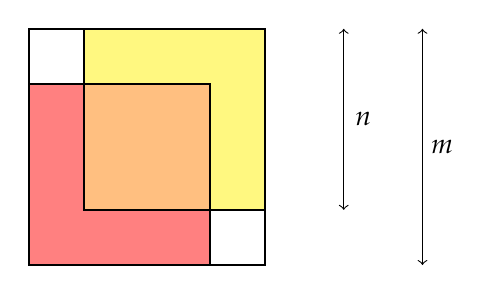
\begin{tikzpicture}
		\draw[thick] (0,0) rectangle (3,3);
		\draw[thick, fill=red!50] (0,0) rectangle (2.3,2.3);
		\draw[thick, fill=yellow!50] (0.7,0.7) rectangle (3, 3);
		\draw[thick, fill=orange!50] (0.7,0.7) rectangle (2.3, 2.3);
		\draw[<->] (4, 0.7)--(4, 3);
		\node at (4.25, 1.85) (n) {$n$};
		\draw[<->] (5, 0)--(5, 3);
		\node at (5.25, 1.5) (m) {$m$};
	\end{tikzpicture}
\end{center}
Omdat $m^2 = 2n^2$, is het stuk waar de twee vierkanten met zijde $n$
over elkaar liggen even groot als het stuk dat door geen van beide
vierkanten wordt bedekt. De oppervlakte van het oranje vierkant is dus
even groot als die van de twee niet-ingekleurde vierkanten samen. Noem de zijde van
het oranje vierkant $p$ en de zijde van elk niet-ingekleurd vierkant
$q$. Dan is $p^2 = 2q^2$. Maar nu is $\sqrt{2} = \nicefrac{p}{q}$,
waarbij $p < m$, $q < n$ en $p, q \in \Nat$. Dat kan niet: we hadden
$m$ en $n$ juist zo klein mogelijk gekozen.
\emph{De tweede manier is formeel.} Uit $m^{2} = 2n^{2}$
volgt dat $m$ even is. (Als $x$ oneven is, kun je makkelijk laten zien
dat $x^2$ ook oneven is.) Dus $m = 2r$ voor een bepaalde $r \in \Nat$. Als we dit
omwerken, krijgen we $2r^2 = n^2$,
		%				\begin{align*}
		%					(2q)^{2} &= 2n^{2}\\
		%					4q^{2} &= 2n^{2}\\
		%					2q^{2} &= n^{2}
		%				\end{align*}
dus ook $n$ is even. Zowel $m$ als $n$ is dus even. De breuk
$\nicefrac{m}{n}$ \emph{kan} daarom toch verder worden vereenvoudigd.
Dat is de tegenspraak.
\end{proof}
Dit bewijs met een plaatje brengt ons trouwens terug bij
\olref[his][set][mythology]{sec}. Tennenbaum (1927--2006) was beslist
een moderne wiskundige. Toch is het bewijs onmiskenbaar mooi en
helemaal waterdicht, en sluit het aan bij ons meetkundige gevoel.
Hoe dan ook: de reële getallen zijn ``uitgebreider'' dan de rationale
getallen. Je kunt zeggen dat de rationale getallen ``gaten'' hebben en
dat de reële getallen die opvullen. Weierstrass zag dat één eigenschap
precies dit verschil beschrijft. Die heet de volledigheidseigenschap:
\emph{Elke niet-lege verzameling reële getallen die een bovengrens
heeft, heeft ook een kleinste bovengrens.}
Je ziet makkelijk dat de rationale getallen deze
volledigheidseigenschap niet hebben. Neem bijvoorbeeld alle rationale
getallen kleiner dan $\sqrt{2}$:
\[
	\Setabs{p \in \Rat}{p^2 < 2 \text{ of }p < 0}
\]
Deze verzameling heeft binnen de rationale getallen een bovengrens.
Alle !!{element}en zijn bijvoorbeeld kleiner dan $3$. Maar wat is de
kleinste bovengrens? We willen `$\sqrt{2}$' zeggen, maar we hebben net
gezien dat $\sqrt{2}$ \emph{niet} rationaal is. Er is ook geen
\emph{kleinste} rationaal getal dat groter is dan $\sqrt{2}$. De
verzameling heeft dus wel een bovengrens, maar geen kleinste
bovengrens. Daarom hebben de rationale getallen de
volledigheidseigenschap niet.
Bij een ononderbroken getallenlijn, het continuüm, verwachten we juist
de volledigheidseigenschap. We willen niet alleen dat $\sqrt{2}$ een
reëel getal is. We willen alle ``gaten'' in de rationale getallenlijn
opvullen, zodat het continuüm zelf geen ``gaten'' meer heeft. Dat is
precies wat volledigheid ons zal geven.
% END ACCEPTED BODY OLP-0044
\endgroup
% END ACCEPTED UNIT OLP-0044

% BEGIN ACCEPTED UNIT OLP-0045 path=translations/nl-gewoon/content/sets-functions-relations/arithmetization/cuts.tex source-sha256=04929643b0c492b865054012424c7344d723bc121b754c3c93d87a2ba2b537d7
\begingroup
\def\olfilename{OLP-0045}
\def\olfilepath{content/sets-functions-relations/arithmetization/}
\hypertarget{unit-OLP-0045}{}
\typeout{PARTIAL-READER-UNIT OLP-0045}
% BEGIN ACCEPTED BODY OLP-0045 body-sha256=4f15bd932b0415445dcaf55f3b6d987824628ef94d721cc469adc861fc44141c
% Part: sets-functions-relations
% Chapter: arithmetization
% Section: cuts
%


\olfileid{sfr}{arith}{cuts}
\olsection{Van $\Rat$ naar $\Real$}
De volledigheidseigenschap zegt eigenlijk dat elk punt $\alpha$ op de
getallenlijn die lijn netjes in twee helften verdeelt. De onderste
helft heeft $\alpha$ als kleinste bovengrens; de bovenste helft heeft
$\alpha$ als grootste ondergrens. Dedekind stelde voor om de reële
getallen uit de rationale getallen te \emph{maken}. Een rationaal getal
kun je schrijven als een breuk van gehele getallen, waarbij de noemer
niet nul is. Dedekind zag een
reëel getal als een \emph{snede} die de rationale getallen in tweeën
deelt. Zo stellen we $\sqrt{2}$ gelijk aan de \emph{snede} tussen de
rationale getallen $< \sqrt{2}$ en de rationale getallen $> \sqrt{2}$.
Dat kunnen we nog wat preciezer opschrijven. Als we de rationale getallen in twee
helften delen, is de \emph{onderste} helft genoeg om te weten welke
verdeling we hebben gemaakt. Daarom gebruiken we de volgende definitie:
\begin{defn}[Snede]
Een \emph{snede} $\alpha$ is een deel van de rationale getallen dat
niet leeg is en ook niet alle rationale getallen bevat. Als er een
getal in zit, zitten alle kleinere rationale getallen er ook in. Er is
geen grootste getal in de snede. Precies opgeschreven is $\alpha$ dus
een snede als:
\begin{enumerate}
	\item \emph{er iets in zit, maar niet alles}: $\emptyset \neq \alpha \subsetneq \Rat$
	\item \emph{alle kleinere getallen er ook in zitten}: voor alle $p,q \in \Rat$ geldt: als $p < q \in \alpha$, dan $p \in \alpha$
	\item \emph{er geen grootste getal is}: voor elke $p \in \alpha$ is er een $q \in \alpha$ waarvoor $p < q$
\end{enumerate}
De verzameling $\Real$ bestaat dan uit alle sneden.
\end{defn}
We kunnen nu dus zeggen dat $\sqrt{2} = \Setabs{p \in \Rat}{p^2 < 2\text{ of }p < 0}$. We moeten nog wel controleren dat dit echt een
\emph{snede} is. Dat doen we pas in \olref[check]{sec}.
Nu we weten wat onze getallen zijn, moeten we vastleggen hoe de
eenvoudige functies en relaties voor die getallen werken. We beginnen
met deze regel:
\begin{align*}
	\alpha \leq \beta \text{ precies dan als }\alpha \subseteq \beta
\end{align*}
Met deze regel voor de volgorde kunnen we het belangrijkste resultaat
\emph{formuleren}: de verzameling sneden heeft de
volledigheidseigenschap. Dat betekent hier het volgende. Als $S$ een
niet-lege verzameling sneden is
en een bovengrens heeft, dan heeft $S$ ook een kleinste bovengrens.
Volledig uitgeschreven: er is een snede $\lambda$ die een bovengrens
van $S$ is, oftewel\ $(\forall \alpha \in S)\alpha \subseteq
\lambda$. Bovendien is $\lambda$ de kleinste snede die dat doet,
oftewel\ $(\forall \beta \in \Real)((\forall \alpha \in S)\alpha \subseteq \beta \lif \lambda \subseteq \beta)$. Dit
is het bewijs:
\begin{thm}\ollabel{realcompleteness}
De verzameling sneden heeft de volledigheidseigenschap.
\end{thm}
\begin{proof}
Neem een willekeurige niet-lege verzameling sneden $S$ met een
bovengrens. Stel $\lambda = \bigcup S$.
%\Setabs{p \in \Rat}{(\exists \alpha \in S)p \in \alpha}$$
We laten eerst zien dat $\lambda$ een snede is:
\begin{enumerate}
\item $S$ is niet leeg. Daarom zit er minstens één snede in
$S$, zodat $\emptyset \neq \lambda$. Alles wat in $S$ zit, is een snede,
dus $\lambda \subseteq \Rat$. Omdat $S$ een bovengrens heeft, is er
een rationaal getal $p \in \Rat$ dat in geen enkele snede $\alpha \in S$
zit. Daarom
is $p\notin \lambda$ en dus $\lambda \subsetneq \Rat$.
\item Neem aan dat $p < q \in \lambda$. Dan is er een snede $\alpha \in S$
waarvoor $q \in \alpha$. Omdat $\alpha$ een snede is, geldt
$p \in \alpha$. Dus $p \in \lambda$.
\item Neem aan dat $p \in \lambda$. Dan is er een snede $\alpha \in S$
waarvoor $p \in \alpha$. Omdat $\alpha$ een snede is, is er een
$q \in \alpha$ waarvoor $p < q$. Dus $q \in \lambda$.
\end{enumerate}
Daarmee is de bewering bewezen. Verder is het duidelijk dat $(\forall \alpha \in S)\alpha
\subseteq \bigcup S = \lambda$, oftewel\ $\lambda$ is een bovengrens van $S$. Neem nu aan dat $\beta \in \mathbb{R}$ ook een bovengrens is, oftewel\ $(\forall \alpha \in S)\alpha \subseteq \beta$. Kies een willekeurige $p \in \Rat$. Als $p \in \lambda$, dan is er een $\alpha \in S$ met $p \in \alpha$, en dus geldt ook $p \in \beta$. Dit geldt voor elk rationaal getal, zodat $\lambda \subseteq \beta$. Daarom is $\lambda$ de \emph{kleinste} bovengrens van $S$.
\end{proof}
We hebben nu dus sneden die aan de volledigheidseigenschap voldoen.
Je kunt dat ook zo zeggen: er zitten geen “gaten” tussen onze sneden.
(Als we nog eens “sneden” zouden maken, maar nu in de reële getallen
in plaats van de rationale, zouden daar geen interessante nieuwe
dingen uit komen.)
Nu moeten we vastleggen hoe de bewerkingen op de reële getallen werken.
Eerst nemen we de rationale getallen op in de reële getallen. We
spreken af dat $p_\Real = \Setabs{q \in \Rat}{q < p}$ voor elke
$p \in \Rat$. Daarna definiëren we:
\begin{align*}
	\alpha + \beta &= \Setabs{p + q}{p \in \alpha \land q \in \beta}\\
%	\alpha - \beta &\defis \Setabs{p - q}{p \in \alpha \land q \in \Rat \setminus \beta}\\
	\alpha \times \beta &=
	\Setabs{p \times q}{0 \leq p \in \alpha \land 0 \leq q \in \beta} \cup 0_\Real & \text{als }\alpha, \beta \geq 0_\Real
%	\alpha \div \beta &\defis
%	\Setabs{\nicefrac{p}{q}}{p \in \alpha \land q \in \Rat \setminus \beta}  & \text{if }\alpha \geq 0_\Real, \beta > 0_\Real
\end{align*}
Verder spreken we voor elk reëel getal af dat nul maal dat getal nul
is en dat het getal maal nul ook nul is. Voor de andere gevallen van
vermenigvuldiging spreken we eerst het volgende af:
\begin{align*}
	-\alpha &= \Setabs{p - q}{p < 0 \land q \notin \alpha}
\end{align*}
Daarna spreken we af:
\begin{align*}
	\alpha \times \beta &\defis
	\begin{cases}
		\mathord{-}\alpha \times \mathord{-}\beta &\text{als }\alpha < 0_\Real\text{ en }\beta < 0_\Real\\
		\mathord{-}(\mathord{-}\alpha \times \beta) &\text{als }\alpha < 0_\Real \text{ en }\beta > 0_\Real\\
		\mathord{-}(\alpha \times \mathord{-}\beta) &\text{als }\alpha > 0_\Real \text{ en }\beta < 0_\Real
	\end{cases}
\end{align*}
We moeten nog controleren dat elk van deze regels altijd een snede
oplevert. Daarna moeten we laten zien dat de zo gemaakte sneden precies
doen wat ze horen te doen. Dat is niet moeilijk, maar het bewijs is wel
lang. Ook dit behandelen we in \olref[check]{sec}.
% END ACCEPTED BODY OLP-0045
\endgroup
% END ACCEPTED UNIT OLP-0045

% BEGIN ACCEPTED UNIT OLP-0046 path=translations/nl-gewoon/content/sets-functions-relations/arithmetization/reflections.tex source-sha256=0b78eca90d451ede3d16c5c2d4ff65fdba45c2eb9308b15b1d9f8d696cde05cf
\begingroup
\def\olfilename{OLP-0046}
\def\olfilepath{content/sets-functions-relations/arithmetization/}
\hypertarget{unit-OLP-0046}{}
\typeout{PARTIAL-READER-UNIT OLP-0046}
% BEGIN ACCEPTED BODY OLP-0046 body-sha256=2f99e9cd124c5b5169da1b1478e3c0b32c415dc562873edcb9e628a9a22c7d4d
% Part: sets-functions-relations
% Chapter: arithmetization
% Section: reflections



\olfileid{sfr}{arith}{ref}
\olsection{Een paar filosofische gedachten}
Tot zover de technische details. Maar wat heeft dat alles opgeleverd?
Eén ding staat vrijwel vast: dit leverde {mooie} zuivere wiskunde op.
Ook kwamen er diepgaande inzichten uit. De volledigheidseigenschap
laat zien wat het doorslaggevende verschil tussen reële en rationale
getallen is. Dat was een diep inzicht. Door precies te beschrijven hoe je
reële getallen als Dedekindsneden opbouwt, krijgt de analyse bovendien een stevige
basis. We weten nu dat een \emph{volledig geordend lichaam} echt kan
bestaan: een getalsysteem met de vereiste rekenregels, volgorde en
volledigheid. De sneden vormen zo'n lichaam.
Toch zijn er een paar redenen om voorzichtig te zijn met deze resultaten.
Ten eerste is het niet duidelijk dat reële getallen als sneden zien
\emph{strenger} is dan ze zien als hun bekende, misschien oneindige
rijen cijfers achter de komma. Die laatste ``opbouw'' lijkt wat op de
opbouw met Cauchyrijen. Toch kenden wiskundigen het idee in wezen al
vanaf het begin van de zeventiende eeuw (zie \olref[cauchy]{sec}). De
echte winst aan strengheid kwam door het inzicht dat de reële getallen de
volledigheidseigenschap hebben. Dat we ze ook als bepaalde
verzamelingen kunnen opbouwen, is op zichzelf misschien niet zo
interessant.
Nog minder duidelijk is of het veel makkelijker opbouwen van de gehele en
rationale getallen binnen de verzamelingenleer het wiskundige werk strenger maakt. Let op wat we in de
praktijk doen. Eerst hebben we de gehele getallen als klassen van
gelijkwaardige geordende paren natuurlijke getallen
\emph{opgebouwd}. Daarna bouwden we de rationale getallen op als zulke
klassen van paren gehele getallen, en de reële getallen als
verzamelingen rationale getallen. Meteen daarna gaan we die hele opbouw
weer \emph{vergeten}. Niemand wil hem tijdens een wiskundig bewijs
\emph{gebruiken}, behalve natuurlijk om te bewijzen dat de opbouw zelf
goed werkt. Rechtstreeks over een reëel getal praten is veel
makkelijker dan praten over een verzameling van verzamelingen van
verzamelingen van verzamelingen van verzamelingen van verzamelingen van
verzamelingen natuurlijke getallen.
%(For reals were constructed as sets of rationals; and these were constructed as equivalence classes of ordered pairs of integers, i.e., sets of sets of sets of integers; etc.).
%2/3 = [2,3]
%	i.e. {<2,3>, ... }
%	{ {{2},{2,3}}, ... }
%
%reals are 
%	sets of rationals 
%
%rationals are 
%	sets of sets of sets of integers
%
%integers are
%	sets of sets of sets of naturals
Het minst geloofwaardig is dat deze definities ons vertellen wat
gehele, rationale en reële getallen \emph{zijn}, \emph{als we vragen
wat ze werkelijk zijn}. Het is dus maar de vraag of reële getallen
bijvoorbeeld \emph{niets anders zijn dan} bepaalde verzamelingen van
verzamelingen van verzamelingen\ldots. Het grootste probleem voor dat idee
is dat we de opbouw op veel andere manieren hadden kunnen doen. Voor de reële getallen bestaan echt
interessante andere manieren (zie \olref[cauchy]{sec}). Maar het kan
ook heel eenvoudig anders. In \olref[sfr][rel][ref]{sec} zagen we dat
we een geordend paar iets anders hadden kunnen definiëren. Met die
andere definitie had alles even goed gewerkt, maar waren er andere
objecten uitgekomen. Er zijn dus meerdere manieren om de gehele,
rationale en reële getallen als verzamelingen op te bouwen. Dan zou het
zomaar een keuze zijn, en nogal gênant, om te beweren dat de gehele
getallen bijvoorbeeld \emph{deze} verzamelingen zijn in plaats van
\emph{die}. (Zoals in \olref[sfr][rel][ref]{sec} is dit een voorbeeld
van een argument dat bekend is geworden door
\citealt{Benacerraf1965}.)
Er is nog iets \emph{vreemds} aan onze opbouw. We begonnen met de
natuurlijke getallen. Daarna bouwden we de gehele getallen, met daarin
``de $0$ van de gehele getallen'': $ \equivrep{0,0}{\Intequiv}$. Maar
$0 \neq \equivrep{0,0}{\Intequiv}$. Volgens deze opbouw is
\emph{geen enkel} natuurlijk getal een geheel getal. Dat gaat sterk
tegen ons gewone idee van getallen in. In
\olref[sfr][set][imp]{sec} zeiden we immers bijna zonder uitleg dat
$\Nat \subseteq \Rat$. Als de opbouw precies vertelt \emph{wat} de
getallen zijn, was meteen duidelijk dat dit niet klopte.
Wat houden we dan over? In een na\"ieve verzamelingenleer kunnen we de
natuurlijke getallen als gegeven nemen en de gehele, rationale en reële
getallen als bepaalde verzamelingen \emph{behandelen}. Zo kunnen we de
theorieën over deze getallen in de verzamelingenleer \emph{onderbrengen}.
Maar wat dat filosofisch betekent, is niet zo eenvoudig.
Dit is natuurlijk niet het laatste woord!{} Het punt is alleen dit. Wie
wil laten zien dat het opbouwen van de reële getallen binnen de
verzamelingenleer filosofisch echt
belangrijk \emph{is}, heeft daar nog een \emph{filosofisch} argument
voor nodig.
%Additionally: for the entire duration of this chapter, we have treated
%the natural numbers as simply \emph{given} to us. But what can we do
%with them? That is the subject matter for the next chapter.
% END ACCEPTED BODY OLP-0046
\endgroup
% END ACCEPTED UNIT OLP-0046

% BEGIN ACCEPTED UNIT OLP-0047 path=translations/nl-gewoon/content/sets-functions-relations/arithmetization/checking-details.tex source-sha256=f80cfdaef7b6ea4c335fb8554d7fc2645c3e6fe9b91afc2cc19cf63bf029e77b
\begingroup
\def\olfilename{OLP-0047}
\def\olfilepath{content/sets-functions-relations/arithmetization/}
\hypertarget{unit-OLP-0047}{}
\typeout{PARTIAL-READER-UNIT OLP-0047}
% BEGIN ACCEPTED BODY OLP-0047 body-sha256=0e825d02aa3b78c47e80bdb3d847f683655e8b917ae25f1fe924ab1697a7479f
% Part: sets-functions-relations
% Chapter: arithmetization
% Section: checking-details
%


	
\olfileid{sfr}{arith}{check}
\olsection{Geordende ringen en lichamen}
In dit hoofdstuk zeiden we een paar keer dat bepaalde definities
``werken zoals het hoort''. In deze technische bijlage leggen we uit
wat dat betekent. We laten ook in grote lijnen zien hoe je kunt
bewijzen dat de definities echt ``goed'' werken.
In \olref[int]{sec} hebben we vastgelegd hoe je de getallen in $\Int$
optelt en vermenigvuldigt. We moeten nu laten zien dat $\Int$ daardoor
de structuur krijgt die we willen. Om precies te zijn: de gehele
getallen moeten samen een commutatieve ring vormen.
\begin{defn}
	Een \emph{commutatieve ring} is een verzameling $S$ met twee speciale elementen, $0$ en $1$, en twee rekenbewerkingen, $+$ en $\times$. De volgende acht formules moeten dan kloppen:
	\begin{align*}
		\emph{Associativiteit (anders groeperen)}&&a + (b+ c) & = (a + b) + c \\
		&& (a \times b) \times c & = a \times (b\times c)\\
		\emph{Commutativiteit (volgorde omwisselen)}&&a + b &= b+ a  \\
		&&  a \times b&= b\times a\\ 
		\emph{Neutrale elementen (0 bij optellen en 1 bij vermenigvuldigen veranderen niets)}&&a + 0 &= a \\
		&& a \times 1 &= a\\
		\emph{Additieve inverse (tegengestelde bij optellen)}&&(\exists b\in S)0&=a + b\\
		\emph{Distributiviteit (vermenigvuldigen over een som)}&&a \times (b+ c ) &= (a \times b) + (a \times c)
	\end{align*}
	Deze formules moeten kloppen voor elke keuze van de letters uit $S$; dat schrijven we er niet elke keer apart bij. Let ook op: de elementen die hier $0$ en~$1$ heten, hoeven niet de natuurlijke getallen nul en één te zijn.
\end{defn}
Om te bewijzen dat de gehele getallen een commutatieve ring vormen,
moeten we dus deze acht regels nalopen. Elke regel op zichzelf is
eenvoudig, maar samen is het nogal wat werk. Hieronder bewijzen we
bijvoorbeeld de \emph{associativiteit} van het optellen: de uitkomst
verandert niet als je de haakjes anders zet.
\begin{proof} 
Kies $i, j, k \in \Int$. We kunnen dan natuurlijke getallen $a_1, b_1,
a_2, b_2, a_3, b_3 \in \Nat$ vinden zodat $i = \equivrep{a_1, b_1}{}$ en $j =
\equivrep{a_2,b_2}{}$ en $k = \equivrep{a_3, b_3}{}$. (Om dit
makkelijker te lezen, schrijven we ``$\equivrep{x, y}{}$'' in plaats van
``$\equivrep{x, y}{\Intequiv}$''. Dat doen we in dit hele
deel.) Nu rekenen we:
\begin{align*}
	i + (j + k) &= \equivrep{a_1, b_1}{}+(\equivrep{a_2, b_2}{} + \equivrep{a_3, b_3}{}) \\
	&= \equivrep{a_1,  b_1}{} + \equivrep{a_2+a_3, b_2+b_3}{}\\
	&= \equivrep{a_1 + (a_2 + a_3), b_1 + (b_2 + b_3)}{}\\
	&= \equivrep{(a_1 + a_2) + a_3, (b_1 + b_2) + b_3}{}\\
	&= \equivrep{a_1 + a_2, b_1 + b_2}{} + \equivrep{a_3, b_3}{}\\
	&= (\equivrep{a_1, b_1}{} + \equivrep{a_2, b_2}{}) + \equivrep{a_3, b_3}{}\\
	&= (i+j) + k
\end{align*}
Hier gebruiken we gewoon de bekende regels voor optellen op $\Nat$.
\end{proof}
Nu laten we zien dat elk geheel getal bij optellen een tegengestelde
heeft, oftewel een \emph{additieve inverse}:
\begin{proof}
Kies $i \in \Int$ en schrijf $i = \equivrep{a,b}{}$ met $a,b \in
\Nat$. Neem $j = \equivrep{b,a}{} \in
\Int$. Voor natuurlijke getallen geldt $(a+b) + 0 = 0 + (b+a)$.
Volgens de definitie betekent dit dat $\tuple{a+b, b+a} \sim_\Int
\tuple{0,0}$, en dus dat $\equivrep{a+b, b+a}{} = \equivrep{0, 0}{}
= 0_\Int$. We krijgen daarom $i + j =
\equivrep{a,b}{}+\equivrep{b,a}{}=\equivrep{a+b, b+a}{}= \equivrep{0,
0}{} = 0_\Int$.
\end{proof}
Hierna bewijzen we de \emph{distributiviteit}: als je met een som
vermenigvuldigt, mag je de vermenigvuldiging over beide termen
verdelen.
\begin{proof}
Kies net als hierboven $i = \equivrep{a_1, b_1}{}$ en $j =
\equivrep{a_2,b_2}{}$ en $k = \equivrep{a_3, b_3}{}$. Dan rekenen we:
\begin{align*}
	i \times (j + k) 
	&= \equivrep{a_1, b_1}{} \times (\equivrep{a_2,b_2}{} + \equivrep{a_3, b_3}{})\\
	&= \equivrep{a_1, b_1}{} \times \equivrep{a_2 + a_3,b_2+b_3}{}\\
	&= \equivrep{a_1  (a_2 + a_3) + b_1  (b_2+b_3), a_1  (b_2 + b_3) + b_1 (a_2 + a_3)}{}\\
	&= \equivrep{a_1 a_2 + a_1a_3 + b_1 b_2+b_1b_3, a_1 b_2 + a_1b_3 + a_2b_1 + a_3b_1}{}\\		
%		&= \equivrep{a_1 a_2 + b_1b_2 + a_1a_3 + b_1 b_2+b_1b_3, a_1 b_2 + a_1b_3 + a_2b_1 + a_3b_1}{}\\		
	&= \equivrep{a_1a_2 + b_1b_2, a_1b_2 + a_2b_1}{} + \equivrep{a_1a_3 + b_1b_3, a_1b_3 + a_3b_1}{}\\
	&= (\equivrep{a_1, b_1}{} \times \equivrep{a_2,b_2}{}) + (\equivrep{a_1, b_1}{} \times  \equivrep{a_3, b_3}{})\\
	&= (i \times j) + (i \times k)
\end{align*}
\end{proof}
De andere vijf regels mag je zelf bewijzen. Als dat is gedaan, weten
we dat $\Int$ een commutatieve ring is. Dus optellen en
vermenigvuldigen werken, met onze definities, zoals ze moeten werken.
\begin{prob}
Bewijs dat $\Int$ een commutatieve ring is.
\end{prob}
Maar we zijn nog niet klaar. We hebben niet alleen vastgelegd hoe
optellen en vermenigvuldigen op $\Int$ werken, maar ook wanneer het
ene getal kleiner dan of gelijk aan het andere is; daarvoor gebruiken
we de ordeningsrelatie $\leq$. Ook die moet werken zoals bedoeld.
Preciezer gezegd moeten we bewijzen dat $\Int$ een \emph{geordende}
ring is.\footnote{Bedenk dat volgens
	\olref[sfr][rel][ord]{def:linearorder} een totale ordening
	een relatie is die reflexief, transitief, antisymmetrisch en samenhangend is.
	In een ordening heet die laatste eigenschap soms
	\emph{trichotomie}. Ze zegt dat voor elke $a$ en $b$ geldt: $a \leq b \lor a
	= b \lor a \geq b$.} 
\begin{defn}
Een \emph{geordende ring} is een commutatieve ring met bovendien een
totale ordening $\leq$. Daarbij moeten deze twee regels gelden:
\begin{align*}
	a \leq b &\lif a + c \leq b + c\\
	(a \leq b \land 0 \leq c) &\lif a \times c \leq b \times c
\end{align*}
\end{defn}
\begin{prob}
Bewijs dat $\Int$ een geordende ring is. 
\end{prob}
Ook dit bewijs kost veel schrijfwerk, maar de stappen zelf zijn
eenvoudig. We laten het aan jou over om te bewijzen dat onze
$\Int$ inderdaad een geordende ring is.
Daarmee zijn we klaar met de gehele getallen. Voor de rationale getallen moeten we
bijna hetzelfde doen. We moeten bewijzen dat ze een geordend
\emph{lichaam} vormen, met onze definities van $+$, $\times$ en
$\leq$:
\begin{defn}\ollabel{orderedfield}
Een \emph{geordend lichaam} is een geordende ring waarvoor ook de volgende regel geldt:
\begin{align*}
	\emph{Multiplicatieve inverse (omgekeerde bij vermenigvuldigen)}& & (\forall a \in S \setminus \{0\})(\exists b \in S) a\times b& = 1
\end{align*}
\end{defn}
Als je eenmaal hebt bewezen dat $\Int$ een geordende ring is, is de
volgende stap niet moeilijk. Je moet alleen veel regels nalopen om
te bewijzen dat $\Rat$ een geordend lichaam is.
\begin{prob}
Bewijs dat $\Rat$ een geordend lichaam is.
\end{prob}
Na de gehele en rationale getallen zijn alleen de reële getallen nog
over. We moeten bewijzen dat $\Real$ een \emph{volledig} geordend
lichaam is. Dat is een geordend lichaam met de
volledigheidseigenschap. In \olref[cuts]{realcompleteness} hebben we
al bewezen dat $\Real$ die eigenschap heeft. We moeten nog wel alle
(saaie) stappen nalopen om te bewijzen dat $\Real$ een geordend
lichaam is.
Voor we aan \emph{die} hoop werk beginnen, moeten we eerst een paar
dingen controleren die ``meteen duidelijk'' lijken. We moeten
bijvoorbeeld zeker weten dat $\alpha + \beta$ volgens onze definitie
zelf weer een \emph{snede} is, voor alle sneden $\alpha$ en $\beta$.
Hier is het bewijs:
\begin{proof}	
Omdat $\alpha$ en $\beta$ allebei sneden zijn, is $\alpha + \beta = \Setabs{p
+ q}{p \in \alpha \land q \in \beta}$ een deelverzameling van $\Rat$ die
niet leeg en niet de hele verzameling is. Stel nu dat $x < p + q$ voor een
$p \in \alpha$ en een $q \in \beta$. Dan is $x - p < q$, zodat $x - p
\in \beta$, en dus $x = p + (x - p) \in \alpha + \beta$. Zodra een
getal in deze verzameling zit, zitten alle kleinere rationale
getallen er dus ook in. Dat wil zeggen dat $\alpha + \beta$ een
beginstuk van $\Rat$ is. Neem tot slot een willekeurig $p + q \in
\alpha + \beta$. Omdat $\alpha$ en $\beta$ allebei sneden zijn, kunnen
we $p_1 \in \alpha$ en $q_1 \in \beta$ vinden met $p < p_1$ en $q <
q_1$. Dan is $p + q < p_1 + q_1 \in \alpha + \beta$. Er zit dus
altijd nog een groter getal in $\alpha + \beta$, zodat deze
verzameling geen grootste element, en dus geen maximum, heeft.
\end{proof}
Met vergelijkbare berekeningen kun je laten zien dat $\alpha - \beta$,
$\alpha \times \beta$ en $\alpha \div \beta$ ook sneden zijn. Bij
delingen moet je het geval waarin $\beta$ de nulsnede is buiten
beschouwing laten. Ook dat bewijs laten we aan jou over.
\begin{prob}
Bewijs dat $\Real$ een geordend lichaam is.
\end{prob}
Er blijft nog één klein punt over. In \olref[cuts]{sec} zeggen we dat
we $\sqrt{2} = \Setabs{p \in \Rat}{p < 0 \text{ of }p^2 < 2}$ kunnen nemen.
We moeten nog bewijzen dat die verzameling echt een \emph{snede} is.
Dat gaat zo:
\begin{proof}
Deze verzameling is duidelijk niet leeg, niet gelijk aan alle
rationale getallen en een beginstuk daarvan. We hoeven dus alleen te
bewijzen dat ze geen grootste element heeft. Neem daarvoor een
willekeurig positief rationaal getal $p$ met $p^2 < 2$ en zet $q =
\frac{2p+2}{p+2}$. Het is genoeg om te laten zien dat zowel $p < q$
als $q^2 < 2$ geldt. Voor $p < q$ rekenen we:
\begin{align*}
	p^2 &< 2\\
	p^2 + 2p &< 2 + 2p\\
	p(p + 2) &< 2 + 2p\\
	p &< \tfrac{2+2p}{p+2} = q
\end{align*}
Voor $q^2 < 2$ rekenen we:
\begin{align*}
	p^2 &< 2\\
	2p^2 + 4p + 2 &< p^2 + 4p+ 4\\
	4p^2 + 8p + 4 &< 2(p^2 + 4p + 4)\\
	(2p+2)^2 & <2(p+2)^2\\
	\tfrac{(2p+2)^2}{(p+2)^2} &< 2\\
	q^2 &< 2
\end{align*}
\end{proof}
% END ACCEPTED BODY OLP-0047
\endgroup
% END ACCEPTED UNIT OLP-0047

% BEGIN ACCEPTED UNIT OLP-0048 path=translations/nl-gewoon/content/sets-functions-relations/arithmetization/cauchy.tex source-sha256=3cc033da20413b1ee39a9d318bdbab477ef397a6a4a50dd35bb6b79b65e8f0d9
\begingroup
\def\olfilename{OLP-0048}
\def\olfilepath{content/sets-functions-relations/arithmetization/}
\hypertarget{unit-OLP-0048}{}
\typeout{PARTIAL-READER-UNIT OLP-0048}
% BEGIN ACCEPTED BODY OLP-0048 body-sha256=16469b1b240249d102f33d7d9534677e125934b3b79f6414534bf03f8b3e22e6
% Part: sets-functions-relations
% Chapter: arithmetization
% Section: cauchy



\olfileid{sfr}{arith}{cauchy}
\olsection{Bijlage: reële getallen opbouwen met Cauchyrijen}
In \olref[cuts]{sec} bouwden we de reële getallen op met
Dedekindsneden. Hier leggen we een andere manier uit. We beginnen bij
de definitie van Cauchy van wat we nu een Cauchyrij noemen. Andere
schrijvers uit de negentiende eeuw gebruikten die definitie om de reële
getallen te \emph{bouwen}. Dat waren vooral Weierstrass, Heine,
M\'{e}ray en Cantor. (Een goed overzicht van deze geschiedenis staat
bij \citeauthor{OConnorRobertson:RN}
\citeyear{OConnorRobertson:RN}.)
Maar eerst gaan we terug naar Simon Stevin (1548--1620). Stevin zag dat
we elk reëel getal kunnen weergeven met de cijfers van zijn
decimaalontwikkeling. Zelfs een irrationaal getal als $\sqrt{2}$ heeft
zo'n rij cijfers. Die begint zo:
\[
	1.41421356237\ldots
\] 
Zo'n rij cijfers past heel makkelijk in de verzamelingenleer. Zie hem
als een functie $d \colon \Nat \to \Nat$. Dan is $d(n)$ het cijfer op
de $n$-de plaats achter de komma waarnaar we kijken. We moeten nog wel
iets toevoegen voor het stuk vóór de komma, hier alleen $1$. Ook
hebben we een equivalentierelatie nodig: een regel die ervoor zorgt dat
verschillende schrijfwijzen voor hetzelfde getal bij elkaar horen. Zo
moet bijvoorbeeld $0.999\ldots = 1$ gelden. Op deze manier kunnen we de
reële getallen in de verzamelingenleer volledig nauwkeurig opbouwen,
op Stevins manier.
Stevin is hier niet ons hoofdonderwerp. (Meer over Stevin staat in
\citealt{KatzKatz2012}.) Maar zijn idee brengt ons dicht bij een andere
mogelijkheid. In plaats van meteen de cijfers van $\sqrt{2}$ te
gebruiken, nemen we een \emph{rij}: een lijst in een vaste volgorde van
steeds nauwkeurigere rationale benaderingen van $\sqrt{2}$. We schrijven
telkens een groter stuk uit:
\[
1, 1.4, 1.414, 1.4142, 1.41421,\ldots
\]
Het idee van ``steeds betere benaderingen'' geeft een paar nieuwe
stappen. Ze lijken op de stappen waarmee we $\Rat$ uit $\Int$ en
$\Int$ uit $\Nat$ bouwden. Dit zijn de belangrijkste:
\begin{enumerate}
	\item Elk reëel getal kun je schrijven als een decimaalontwikkeling.
	Die kan een oneindige rij cijfers hebben.
	\item Dezelfde informatie kun je vastleggen met een rij rationale
	getallen.
	\item Zo'n rij rationale getallen kun je zien als een functie van
	$\Nat$ naar $\Rat$. Neem gewoon $f(n)$ als het $n$-de rationale getal
	in de rij.
\end{enumerate}
Maar niet \emph{elke} functie van $\Nat$ naar $\Rat$ geeft een reëel
getal. Neem bijvoorbeeld deze functie:
\[
	f(n) =\begin{cases}
			1 & \text{als }n\text{ oneven is}\\
			0 &\text{als }n\text{ even is}
		\end{cases}
\]
De rij $0,1,0,1,0,1,0,\ldots$ komt niet steeds dichter bij één reëel
getal. We willen alleen rijen gebruiken die dat wel doen. Daarom kijken
we alleen naar rijen met een \emph{limiet}: een getal waar de termen
uiteindelijk zo dicht bij komen als je maar wilt.
In \olref[his][set][limits]{sec} kwamen we een limiet al tegen. Toch
kunnen we hier niet \emph{helemaal} dezelfde definitie gebruiken. In
``$(\forall \epsilon>0)$'' liep de variabele stilzwijgend over de reële
getallen. Ook keken we daar naar functies op reële getallen. Als we die
definitie nu gebruiken, nemen we de reële getallen dus al aan. Maar die
proberen we juist te \emph{bouwen}. Gelukkig kunnen we een bijna gelijk
idee gebruiken.
\begin{defn}\ollabel{def:CauchySequence}
  Een functie $f: \Nat \to \Rat$ heet een \emph{Cauchyrij} precies als
  voor elk positief getal $\epsilon \in \Rat$ geldt: $(\exists \ell
  \in \Nat)(\forall m, n > \ell)|f(m) - f(n)| < \epsilon$.
\end{defn}
Het idee blijft hetzelfde. Kies hoe nauwkeurig je wilt zijn; dat meten
we met~$\epsilon$. Daarna is er een ``gebied'' waarin je moet kijken:
alle invoeren groter dan~$\ell$. Onze rij $1$, $1.4$, $1.414$,
$1.4142$, $1.41421$\ldots heeft duidelijk een limiet. Wil je
$\sqrt{2}$ benaderen met een fout van minder dan
$\nicefrac{1}{10^{n}}$, dan is elke term na de $n$-de nauwkeurig genoeg.
Je zou nu kunnen zeggen dat elk reëel getal gewoon een Cauchyrij
\emph{is}. Maar net als bij onze opbouw van $\Int$ en $\Rat$ is dat te
na\"ief. Verschillende Cauchyrijen kunnen hetzelfde reële getal
aangeven. Dat zie je zo. Neem een Cauchyrij~$f$. Maak $g$ precies gelijk
aan~$f$, behalve dat $g(0)\neq f(0)$. Na het eerste getal zijn de twee
rijen overal gelijk. Uiteindelijk willen we dus zeggen dat ze dezelfde
limiet hebben, in de betekenis van \olref{def:CauchySequence}. Ze
``definiëren'' dan hetzelfde reële getal. Daarom moeten we die twee
Cauchyrijen als hetzelfde reële getal zien.
Daarom moeten we weer een equivalentierelatie maken voor de
Cauchyrijen: een regel die zegt welke rijen bij elkaar horen. Daarna
stellen we reële getallen gelijk aan klassen van Cauchyrijen die volgens
die regel bij elkaar horen. Eerst moeten
we zeggen wanneer een functie uiteindelijk naar $0$ gaat. Neem een
functie $h : \Nat \to \Rat$. We zeggen dat \emph{$h$ naar $0$ gaat}
precies als voor elk positief getal $\epsilon \in \Rat$ geldt:
$(\exists \ell \in \Nat)(\forall n > \ell)|h(n)| <
\epsilon$.\footnote{Vergelijk dit met de definitie van $\lim_{x
\mathord{\rightarrow}\infty}f(x) = 0$ in
\olref[his][set][limits]{sec}.} Neem verder functies $f$ en $g$ van
$\Nat \to \Rat$ en stel $(f-g)(n) = f(n) - g(n)$. Nu leggen we vast:
\[
	f \Realequiv g \text{ precies als $(f-g)$ naar $0$ gaat}.
\]
We moeten nog nagaan dat $\Realequiv$ echt een equivalentierelatie is.
Dat klopt. Daarna kunnen we de reële getallen zien als de klassen van
Cauchyrijen die volgens $\Realequiv$ bij elkaar horen, voor alle
Cauchyrijen van $\Nat \to \Rat$.
\begin{prob}
Neem $f(n) = 0$ voor elke $n$. Neem $g(n) = \frac{1}{(n+1)^2}$. Laat
zien dat beide functies Cauchyrijen zijn en allebei limiet $0$ hebben.
Daarom geldt ook $f \sim_\Real g$.
\end{prob}
Zoals altijd schrijven we $\equivrep{f}{\Realequiv}$ voor de klasse
waarin $f$ !!a{element} is. Om de tekst leesbaar te houden, laten we de
index hierna weg. We schrijven dus alleen $\equivrep{f}{}$. Ook spreken
we af dat voor elke $q \in \Rat$ geldt: $q_{\Real} =
\equivrep{c_{q}}{}$. Hier is $c_{q}$ de constante functie waarvoor
$c_q(n) = q$ voor elke $n \in \Nat$. Daarna definiëren we de gewone
relaties en rekenbewerkingen voor reële getallen, bijvoorbeeld:
\begin{align*}
	\equivrep{f}{} + \equivrep{g}{} &= 	\equivrep{(f + g)}{} \\
	\equivrep{f}{} \times 	\equivrep{g}{} &= \equivrep{(f \times g)}{} 
\end{align*}
Hierbij is $(f + g)(n) = f(n) + g(n)$ en $(f \times g)(n) = f(n)
\times g(n)$. We moeten ook nagaan dat $(f + g)$, $(f-g)$ en $(f\times
g)$ weer Cauchyrijen zijn als $f$ en $g$ dat zijn. Dat klopt; het
bewijs laten we als oefening.
Tot slot leggen we vast wanneer het ene getal kleiner is dan het andere. We noemen $\equivrep{f}{}$
\emph{positief} precies als $\equivrep{f}{}\neq 0_\Real$ én $(\exists
\ell \in \Nat)(\forall n > \ell)0 < f(n)$. Daarna zeggen we dat
$\equivrep{f}{} < \equivrep{g}{}$ precies als $\equivrep{(g - f)}{}$
positief is. We moeten nagaan dat deze regel altijd dezelfde uitkomst
geeft. Hij mag dus niet afhangen van welke functie uit de klasse we kiezen.
%\begin{align*}
%	\equivrep{f}{} \leq \equivrep{g}{} \text{ iff }&\equivrep{f}{} = \equivrep{g}{} \text{ or }\\
%	&(\exists \ell \in \Nat)(\forall n \in \Nat)(\ell < n \lif f(n) \leq g(n))
%\end{align*}
Als dat klaar is, kunnen we vrij makkelijk laten zien dat de gewone
rekenregels gelden:
\begin{thm}\ollabel{thm:cauchyorderedfield}
De Cauchyrijen vormen een geordend lichaam.
\end{thm}
\begin{proof}
Oefening.
\end{proof}
\begin{prob}
Bewijs dat de Cauchyrijen een geordend lichaam vormen.
\end{prob}
Het is lastiger om te bewijzen dat de reële getallen die we zo hebben
gebouwd de volledigheidseigenschap hebben. Daarom geven we dat bewijs.
\begin{thm}
Elke niet-lege verzameling Cauchyrijen die een bovengrens heeft, heeft
ook een kleinste bovengrens.
\end{thm}
\begin{proof}[Schets van het bewijs] Neem een niet-lege verzameling
Cauchyrijen $S$ met een bovengrens. Er is dus een $p \in \Rat$ waarvoor
$p_{\Real}$ een bovengrens van $S$ is. Neem $r \in S$; dan is er een
$q \in \Rat$ waarvoor $q_{\Real} < r$. Als $S$ een kleinste bovengrens
heeft, ligt die dus tussen $q_\Real$ en $p_\Real$. De twee grenspunten
tellen mee.
We komen steeds dichter bij de kleinste bovengrens door haar tegelijk
van onderen en van boven te benaderen. We maken daarvoor twee functies,
$f, g \colon \Nat \to \Rat$. De functie $f$ moet de kleinste
bovengrens\ van bovenaf benaderen en $g$ van onderaf. We beginnen met:
\begin{align*}
	f(0) &= p \\
	g(0) &= q
\end{align*}
Neem daarna $a_n = \frac{f(n) + g(n)}{2}$ en leg het volgende
vast:\footnote{Dit is een recursieve definitie: elke volgende stap
gebruikt de vorige. Maar we hebben \emph{nog} niet laten zien waarom
zo'n definitie mag.}
\begin{align*}
	f(n+1) &=
	\begin{cases}
		a_n &\text{als }(\forall h \in S)\equivrep{h}{} \leq (a_n)_\Real\\
		f(n)&\text{anders}
	\end{cases}\\
	g(n+1) &=
	\begin{cases}
		a_n &\text{als }(\exists h \in S)\equivrep{h}{} \geq (a_n)_\Real\\
	 	g(n) &\text{anders}
	\end{cases}
\end{align*}
Zowel $f$ als $g$ is een Cauchyrij. (Dat kun je vrij makkelijk
nagaan; we laten het als oefening.) De functie $(f-g)$ gaat naar $0$,
want het verschil tussen $f$ en $g$ is na elke stap hoogstens half zo groot.
Daarom is $\equivrep{f}{} = \equivrep{g}{}$.
Eerst laten we zien dat $\equivrep{f}{}$ een bovengrens van $S$ is.
Dat betekent\ dat $(\forall h \in S)\equivrep{h}{} \leq
\equivrep{f}{}$. (Onderweg gebruiken we
\olref{thm:cauchyorderedfield}.) Neem $h \in S$ en stel, om een
tegenspraak te krijgen, dat $\equivrep{f}{} < \equivrep{h}{}$. Dan is
$0_\Real < \equivrep{(h-f)}{}$. De Cauchyrij $f$ blijft gelijk of
daalt. Daarom is er een $n \in \Nat$ waarvoor
$\equivrep{(c_{f(n)} - f)}{} < \equivrep{(h-f)}{}$. Dus:
\[
	(f(n))_\Real = \equivrep{c_{f(n)}}{} < \equivrep{f}{} + \equivrep{(h-f)}{} = \equivrep{h}{},
\]
maar volgens onze bouw geldt juist $\equivrep{h}{} \leq
(f(n))_\Real$. Dat is een tegenspraak.
Nu laten we zien dat $\equivrep{f}{} = \equivrep{g}{}$ de
\emph{kleinste} bovengrens van $S$ is. Neem een willekeurige Cauchyrij
$j$ en stel dat $\equivrep{j}{} < \equivrep{g}{}$. Net als hierboven
volgt, omdat $g$ \emph{gelijk blijft of stijgt}, dat er een $n \in \Nat$ is
waarvoor $\equivrep{j}{} < (g(n))_\Real$. Maar door onze bouw is er een
$h \in S$ waarvoor $(g(n))_\Real \leq \equivrep{h}{}$. Dus
$\equivrep{j}{} < \equivrep{h}{}$. Daarom is $\equivrep{j}{}$ geen
bovengrens van $S$.
\end{proof}
% END ACCEPTED BODY OLP-0048
\endgroup
% END ACCEPTED UNIT OLP-0048
\OLEndChapterHook

% BEGIN ACCEPTED UNIT OLP-0049 path=translations/nl-gewoon/content/sets-functions-relations/infinite/infinite.tex source-sha256=a29f953c08bb765266c461a8d7e0405712355968e8f052a659fef2be5028e9fb
\begingroup
\def\olfilename{OLP-0049}
\def\olfilepath{content/sets-functions-relations/infinite/}
\hypertarget{unit-OLP-0049}{}
\typeout{PARTIAL-READER-UNIT OLP-0049}
% BEGIN ACCEPTED BODY OLP-0049 body-sha256=f6980accf65c05a4ba7f4b4465ba25ae386c8205bb7c4291ccc86d26dac0f2a6
% Part: sets-functions-relations
% Chapter: infinite



\olchapter{sfr}{infinite}{Oneindige verzamelingen}

\begin{editorial}
Dit hoofdstuk gaat over oneindige verzamelingen. De tekst komt uit Tim
Buttons \emph{Open Set Theory}.
\end{editorial}
% END ACCEPTED BODY OLP-0049
\endgroup
% END ACCEPTED UNIT OLP-0049

% BEGIN ACCEPTED UNIT OLP-0050 path=translations/nl-gewoon/content/sets-functions-relations/infinite/hilberts-hotel.tex source-sha256=6f1187564149e624e7942082b46b49e1baf05ffccdacc8ef0ec6c7164eec01de
\begingroup
\def\olfilename{OLP-0050}
\def\olfilepath{content/sets-functions-relations/infinite/}
\hypertarget{unit-OLP-0050}{}
\typeout{PARTIAL-READER-UNIT OLP-0050}
% BEGIN ACCEPTED BODY OLP-0050 body-sha256=1978f5d8fa64fe63523a87a6d0e9356bd476bc49f381900cf06cf75b2f8c6832
% Part: sets-functions-relations
% Chapter: infinite
% Section: hilberts-hotel
%


\olfileid{sfr}{infinite}{hilbert}
\olsection{Hilberts hotel}

De verzameling natuurlijke getallen is duidelijk oneindig. Maar als we
niet zomaar \emph{willen uitgaan van de natuurlijke getallen}, moeten
we eerst uitleggen wat een oneindige verzameling is, zonder die getallen
zelf te noemen. Hilbert liet in een lezing uit 1924 zien hoe dat kan.
Hij vraagt ons het volgende voor te stellen:
\begin{quote}
[\ldots] een hotel met maar een eindig aantal kamers. In elke kamer
moet precies één gast verblijven. Als de gasten dan op welke manier ook
van kamer wisselen, [maar] er nog steeds niet meer dan één persoon in
elke kamer zit, komt er geen kamer vrij. De hoteleigenaar kan zo geen
plek maken voor een gast die net aankomt [\ldots
\textparagraph \ldots]

Nu spreken we af dat het hotel oneindig veel genummerde kamers heeft:
$1$, $2$, $3$, $4$, $5$, \dots. In elke kamer verblijft precies één
gast. Zodra er een nieuwe gast aankomt, hoeft de eigenaar iedere gast
die er al was alleen naar de kamer met het eerstvolgende nummer te
verhuizen. Dan is kamer~$1$ vrij voor de nieuwe gast.
	\begin{center}
		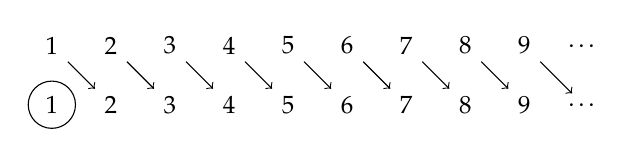
\begin{tikzpicture}[scale = .75]
		\foreach \x in {1, 2, 3, 4, 5, 6, 7, 8, 9}
		{
			\node (\x a) at (\x, 1) {\small{\x}};
			\node (\x b) at (\x, 2) {\small{\x}};
		}
		\node (dotsa) at (10, 1) {\small{\ldots}};
		\node (dotsb) at (10, 2) {\small{\ldots}};
		\draw[->] (1b)--(2a);
		\draw[->] (2b)--(3a);
		\draw[->] (3b)--(4a);
		\draw[->] (4b)--(5a);
		\draw[->] (5b)--(6a);
		\draw[->] (6b)--(7a);
		\draw[->] (7b)--(8a);
		\draw[->] (8b)--(9a);
		\draw[->] (9b)--(dotsa);
		\draw (1,1) circle (.4);
		\end{tikzpicture}
	\end{center}
	(gepubliceerd in \citealt[730]{EwaldSieg2013}; onze vertaling)
\end{quote}
Waar het om gaat, is dat Hilberts hotel oneindig veel kamers heeft. Met
zijn uitleg kunnen we vastleggen wat dat betekent. Dit is ook de aanpak
van Dedekind (we leggen Dedekind hier natuurlijk uit met een voorbeeld
dat pas veel later kwam; zijn definitie stamt uit
\citeyear{Dedekind1888}):

\begin{defn}\ollabel{defn:DedekindInfinite}
Een verzameling $A$ heet \emph{Dedekind-oneindig} precies als er een
injectie van~$A$ naar een echte deelverzameling van~$A$ bestaat. Bij
een injectie krijgen verschillende invoeren verschillende uitkomsten;
de deelverzameling is echt als zij niet de hele oorspronkelijke
verzameling is. Er ontbreekt dan minstens één element.
Anders gezegd: er is een $o \in A$ en een injectie $f \colon A \to A$
waarvoor $o \notin \ran{f}$.
\end{defn}
% END ACCEPTED BODY OLP-0050
\endgroup
% END ACCEPTED UNIT OLP-0050

% BEGIN ACCEPTED UNIT OLP-0051 path=translations/nl-gewoon/content/sets-functions-relations/infinite/dedekind-algebra.tex source-sha256=8203b6d054af11c5b706bec52d7ae333a8e654440c0692790ff4cc18d6cce0b5
\begingroup
\def\olfilename{OLP-0051}
\def\olfilepath{content/sets-functions-relations/infinite/}
\hypertarget{unit-OLP-0051}{}
\typeout{PARTIAL-READER-UNIT OLP-0051}
% BEGIN ACCEPTED BODY OLP-0051 body-sha256=039200960d39f238ac68d49120527cb8543059fee0cbc2889e7dfdc94bd30060
% Part: sets-functions-relations
% Chapter: infinite
% Section: dedekind
%


\olfileid{sfr}{infinite}{dedekind}
\olsection{Dedekindalgebra's}

De natuurlijke getallen moeten niet alleen oneindig zijn. Ze moeten ook
bepaalde (algebraïsche) eigenschappen hebben, zodat optellen,
vermenigvuldigen enzovoort goed werken.

Dedekind nam de \emph{opvolgerfunctie} als uitgangspunt. Die functie
stuurt elk getal naar zijn opvolger. Daarna beschreef hij de getallen
met deze drie eigenschappen:
\begin{enumerate}
	\item Er is een getal, $0$, dat niet de opvolger van een getal is
	\\anders gezegd: $0 \notin \ran{s}$
	\\in symbolen: $\forall x\ s(x) \neq 0$
	\item Verschillende getallen hebben verschillende opvolgers
	\\dus is $s$ injectief: verschillende invoeren krijgen verschillende uitkomsten
	\\in symbolen: $\forall x \forall y (s(x) = s(y) \lif x = y)$
	\item\ollabel{repeatedapplication} Elk getal krijg je door bij $0$ te
	beginnen en steeds de opvolgerfunctie toe te passen.
\end{enumerate}
De eerste twee eigenschappen kunnen we makkelijk in eerste-ordelogica
opschrijven (zie hierboven). Maar voor \olref{repeatedapplication}
hebben we meer nodig dan alleen eerste-ordelogica. Dedekind wist deze
eigenschap, \olref{repeatedapplication}, als volgt met verzamelingen te
omschrijven:
\begin{enumerate}
	\item[3$'$.] De natuurlijke getallen vormen de kleinste verzameling
	die \emph{gesloten is onder de opvolgerfunctie}. Dat betekent: pas je
	$s$ toe op een willekeurig element van de verzameling, dan krijg je
	opnieuw een element van die verzameling.
\end{enumerate}
We moeten dit nu precies uitschrijven.

\begin{defn}\ollabel{Closure}
	Neem een functie $f$. We noemen een verzameling $X$ $f$-\emph{gesloten}
	{precies als} $(\forall x \in X)f(x) \in X$. De functie brengt
	elementen van die verzameling dan niet buiten de verzameling. Voor
	elke $o$ leggen we nu vast:
	$$\closureofunder{f}{o} = \bigcap\Setabs{X}{o \in X\text{ en }X
\text{ $f$-gesloten is}}$$
\end{defn}

Dus $\closureofunder{f}{o}$ is de doorsnede van alle $f$-gesloten
verzamelingen waar $o$ een element van is: het deel dat al die
verzamelingen gemeen hebben. Daarom is $\closureofunder{f}{o}$
intuïtief de \emph{kleinste} $f$-gesloten verzameling waar $o$ een
element van is. Het volgende resultaat maakt dat precies:
\begin{lem}\ollabel{closureproperties}
	Voor elke verzameling $A$, elke functie $f \colon A \to A$ en elke
	$o \in A$:
	\begin{enumerate}
		\item\ollabel{closurehaselem} $o \in \closureofunder{f}{o}$; en
		\item\ollabel{closureclosed} $\closureofunder{f}{o}$ is $f$-gesloten; en
		\item\ollabel{closuresmallest} als $X$ $f$-gesloten is en $o \in
		X$, dan $\closureofunder{f}{o} \subseteq X$
	\end{enumerate}
\end{lem}

\begin{proof}
Er is minstens één $f$-gesloten verzameling waar $o$ een element van
is, namelijk $\ran{f}\cup \{o\}$. Daarom bestaat
$\closureofunder{f}{o}$, de doorsnede van \emph{alle} zulke
verzamelingen. We moeten nu
\olref{closurehaselem}--\olref{closuresmallest} nalopen.

Voor \olref{closurehaselem}: $o \in \closureofunder{f}{o}$. Alle
verzamelingen in de doorsnede hebben $o$ als element, dus hun doorsnede
ook.

Voor \olref{closureclosed}: neem $x \in \closureofunder{f}{o}$. Als
$o \in X$ en $X$ $f$-gesloten is, dan zit $x \in X$ en zit ook
$f(x) \in X$, want $X$ is $f$-gesloten. Dit geldt voor elke verzameling
in de doorsnede, dus $f(x) \in \closureofunder{f}{o}$.

Voor \olref{closuresmallest} gebruiken we een algemene regel: als
$X \in C$, dan $\bigcap C \subseteq X$.
\end{proof}

Nu kunnen we de volgende definitie geven:

\begin{defn}
Een \emph{Dedekindalgebra} bestaat uit drie dingen: een verzameling
$A$, een functie $f \colon A \to A$ en een gekozen element $o \in A$.
Ze moeten aan deze voorwaarden voldoen:
	\begin{enumerate}
		\item \ollabel{ded:proper} $o \notin \ran{f}$
		\item \ollabel{ded:injection} $f$ is injectief
		\item \ollabel{ded:closure} $A = \closureofunder{f}{o}$
	\end{enumerate}
\end{defn}

Omdat $A = \closureofunder{f}{o}$, weten we uit het vorige resultaat
dat $A$ de kleinste $f$-gesloten verzameling is waar $o$ een element
van is. Elke Dedekindalgebra is Dedekind-oneindig. Dat zie je direct aan
voorwaarden \olref{ded:proper} en \olref{ded:injection} van de
definitie. Maar er geldt ook iets in de omgekeerde richting: van elke
Dedekind-oneindige verzameling kunnen we een Dedekindalgebra maken.

\begin{thm}\ollabel{thm:DedekindInfiniteAlgebra}
Als er een Dedekind-oneindige verzameling bestaat, dan bestaat er een
Dedekindalgebra.
\end{thm}

\begin{proof}
Neem een Dedekind-oneindige verzameling $D$. Er is dan een injectie $g
\colon D \to D$ en een element $o \in D \setminus \ran{g}$. Neem nu
$A = \closureofunder{g}{o}$. Volgens \olref{closureproperties} bestaat
$A$ en geldt $o \in A$. Neem $f = \funrestrictionto{g}{A}$. We laten
zien dat $A, f, o$ samen een Dedekindalgebra vormen.

Voor \olref{ded:proper}: $o \notin \ran{g}$ en $\ran{f} \subseteq
\ran{g}$, dus $o\notin \ran{f}$.

Voor \olref{ded:injection}: $g$ is een injectie op $D$ en $f
\subseteq g$, dus is de beperking ook injectief.

Voor \olref{ded:closure}: volgens \olref{closureproperties} is $A$
$g$-gesloten; dus is $A$ ook $f$-gesloten. Daarom is
$\closureofunder{f}{o} \subseteq A$ volgens
\olref{closureproperties}. Verder is $\closureofunder{f}{o}$ zelf
$f$-gesloten en geldt $f = \funrestrictionto{g}{A}$. Daaruit volgt dat
$\closureofunder{f}{o}$ ook $g$-gesloten is. Dus
$A \subseteq \closureofunder{f}{o}$ volgens
\olref{closureproperties}.
\end{proof}
% END ACCEPTED BODY OLP-0051
\endgroup
% END ACCEPTED UNIT OLP-0051

% BEGIN ACCEPTED UNIT OLP-0052 path=translations/nl-gewoon/content/sets-functions-relations/infinite/dedekind-induction.tex source-sha256=6d2a60b4b69234a23877ebf4d6316c8c26e166b36c58231fe9df277d4d13a7cd
\begingroup
\def\olfilename{OLP-0052}
\def\olfilepath{content/sets-functions-relations/infinite/}
\hypertarget{unit-OLP-0052}{}
\typeout{PARTIAL-READER-UNIT OLP-0052}
% BEGIN ACCEPTED BODY OLP-0052 body-sha256=ef4ec8b107d172568fd2f7dc1cfcdf98b5895fe747cc4905479ef9d8bcfc7a1c
% Part: sets-functions-relations
% Chapter: infinite
% Section: dedekind-induction



\olfileid{sfr}{infinite}{induction}
\olsection[Volledige inductie]{Dedekindalgebra's en volledige inductie}

Nu komt het belangrijkste punt: een Dedekindalgebra---\emph{elke}
Dedekindalgebra---kan de rol van de natuurlijke getallen overnemen. Dat
volgt meteen uit dit eenvoudige resultaat:

\begin{thm}[Volledige inductie]\ollabel{thm:dedinfiniteinduction}
Laat $N, s, o$ samen een Dedekindalgebra vormen. Neem een willekeurige
verzameling $X$. Dan geldt:
	\begin{center}
		als $o \in X$ en $(\forall {n} \in N \cap X){s}({n}) \in X$, {dan} $N \subseteq X$.
	\end{center}
\end{thm}

\begin{proof}
Volgens de definitie van een Dedekindalgebra is $N =
\closureofunder{s}{o}$. Stel nu dat ${o} \in X$ en $(\forall {n} \in
N)(n \in X \lif {s}({n}) \in X)$. Het gekozen element ligt ook in
de verzameling van de algebra, en dus geldt ${o} \in N \cap X$.
Neem nu ${n} \in N \cap X$.
Volgens de aanname geldt ${s}({n}) \in X$. Ook geldt
${s}({n}) \in N$, omdat $s \colon N \to N$. Dus is $N \cap X$
$s$-gesloten. Deze verzameling bevat het gekozen element. Zij bevat dus
ook de kleinste gesloten verzameling met dat element. Daarom is $N =
\closureofunder{s}{o} \subseteq X$.
\end{proof}

Inductie is een kenmerkende eigenschap van de natuurlijke getallen.
Daarom kunnen we van elke Dedekind-oneindige verzameling een
Dedekindalgebra maken en die algebra de rol van de natuurlijke getallen
laten spelen.

\olref{thm:dedinfiniteinduction} beschrijft inductie met
\emph{verzamelingstheoretische} begrippen. We kunnen dezelfde regel
ook in een bekende vorm opschrijven:

\begin{cor}\ollabel{natinductionschema}
Laat $N, s, o$ samen een Dedekindalgebra vormen. Neem een formule
$\phi(x)$ waarin parameters mogen voorkomen. Dan geldt:
\begin{center}
	als $\phi(o)$ en $(\forall {n} \in N)(\phi(n)\lif
	\phi({s}({n})))$, {dan} $(\forall n \in N)\phi(n)$
\end{center}
\end{cor}

\begin{proof}
Neem $X = \Setabs{n \in N}{\phi(n)}$ en gebruik nu
\olref{thm:dedinfiniteinduction}.
\end{proof}

Hierboven zeiden we dat een formule ``parameters mag hebben''. Grofweg
betekent dit dat we voor elke keuze van objecten $c_1, \ldots, c_k$
mogen werken met $\phi(x, c_1, \ldots, c_k)$. We kunnen hetzelfde ook
precies opschrijven zonder het woord ``parameters''. Neem een formule
$\phi(x, v_1, \ldots, v_k)$ en schrijf al haar vrije variabelen erbij.
Dan geldt:
	\begin{align*}
			\forall v_1 \ldots \forall v_k((&\phi(o, v_1,\ldots, v_k) \land {}\\
			&	(\forall x \in N)(\phi(x,v_1, \ldots, v_k) \lif \phi(s(x), v_1,\ldots, v_k))) \lif {}\\
			&\hspace{3em} (\forall x \in N)\phi(x, v_1,\ldots, v_k))
	\end{align*}
De woorden ``met parameters'' maken dit duidelijk veel makkelijker te
lezen. (In \olref[sth][][]{part} zullen we deze manier van spreken vaak
gebruiken.)

Terug naar Dedekindalgebra's. Voor elke Dedekindalgebra kunnen we ook
de gewone rekenfuncties voor optellen, vermenigvuldigen en
machtsverheffen vastleggen. Dat is niet eenvoudig. We hebben daarvoor
de techniek van de \emph{recursieve definitie} nodig. Die techniek
leggen we pas veel later uit en rechtvaardigen we daar in een veel
algemenere situatie. (Wie nieuwsgierig is, kan dit deel na
\olref[sth][ord-arithmetic][]{chap} nog eens lezen, of een andere uitleg
bekijken, zoals \citealt[pp.~95--8]{Potter2004}.) Als $N, s, o$ samen
een Dedekindalgebra vormen, kunnen we uiteindelijk deze regels
vastleggen:
\begin{align*}
	{a} + {o} &= {a} & & & {a} \times {o} &= {o} & & & {a}^{o} &= s(o)\\
{a} + {s}({b}) &= {s}({a}+{b}) &&& {a} \times {s}({b}) &= ({a}\times {b}) + {a}  & & & {a}^{{s}({b})} &= {a}^{b} \times {a}
\end{align*}
Daarna kunnen we laten zien dat deze rekenfuncties werken zoals we
verwachten.
% END ACCEPTED BODY OLP-0052
\endgroup
% END ACCEPTED UNIT OLP-0052

% BEGIN ACCEPTED UNIT OLP-0053 path=translations/nl-gewoon/content/sets-functions-relations/infinite/dedekinds-proof.tex source-sha256=69e5a22b57964ea2a1a1edf0f91c6175593d551776896905eb3bb9cbcfc47b53
\begingroup
\def\olfilename{OLP-0053}
\def\olfilepath{content/sets-functions-relations/infinite/}
\hypertarget{unit-OLP-0053}{}
\typeout{PARTIAL-READER-UNIT OLP-0053}
% BEGIN ACCEPTED BODY OLP-0053 body-sha256=204106aa9616f73f1484708cadc725354b97d0f68fcb18524ccfd452c6f8ba2c
% Part: sets-functions-relations
% Chapter: infinite
% Section: dedekinds-proof
%


\olfileid{sfr}{infinite}{dedekindsproof}

\olsection[Dedekinds ``bewijs'']{Dedekinds ``bewijs'' dat er een
oneindige verzameling bestaat}

In dit hoofdstuk hebben we de natuurlijke getallen met verzamelingen
beschreven. Daarbij gebruikten we Dedekindalgebra's. In
\olref[arith][ref]{sec} bespraken we onder meer wat de aritmetisering
van de analyse filosofisch betekent: de analyse wordt in rekenkundige
termen opgebouwd. Nu moeten we bekijken wat het resultaat van dit
hoofdstuk betekent.

In heel \olref[sfr][arith][]{chap} gingen we uit van de natuurlijke
getallen en lieten we precies zien hoe we daarmee de gehele, rationale
en reële getallen konden opbouwen. In dit hoofdstuk hebben we de
natuurlijke getallen zelf niet op die manier opgebouwd. We hebben
alleen laten zien dat we \emph{van elke Dedekind-oneindige verzameling}
een verzameling kunnen definiëren die precies de eigenschappen heeft die
we van~$\Nat$ verlangen.

We kunnen dus niet beweren dat we een metafysische vraag hebben
beantwoord, bijvoorbeeld: \emph{welke objecten zijn de natuurlijke
getallen}? Dat is maar goed ook. In
\olref[sfr][arith][ref]{sec} zeiden we immers dat we de definitie
van~$\Real$ als de verzameling van Dedekindsneden niet als een
\emph{ontdekking} moeten zien. Het is een handige afspraak. Waar het om
gaat, is dat Dedekindsneden de belangrijkste wiskundige eigenschappen
van de reële getallen hebben. Hier geldt hetzelfde: \emph{elke}
Dedekindalgebra heeft de belangrijkste wiskundige eigenschappen van de
natuurlijke getallen. (Dedekind maakte dit extra duidelijk door te
bewijzen dat alle Dedekindalgebra's \emph{isomorf} zijn
(\citeyear[stellingen 132--3]{Dedekind1888}). Geen wonder dat veel
hedendaagse ``structuralisten'' Dedekind daarom als voorloper noemen.)

We hebben ook laten zien hoe we de theorie van de natuurlijke getallen
kunnen onderbrengen in een eenvoudige, na\"ieve verzamelingenleer. Die
leer is nog vrij informeel. Maar ze lijkt de natuurlijke getallen niet
vooraf als gegeven aan te nemen. Misschien komen we zo dichter bij
Dedekinds eigen ambitieuze plan. Hij legde het zo uit:
\begin{quote}
	Als iets bewezen kan worden, mogen we het in de wetenschap niet zonder
	bewijs geloven. Dat lijkt een redelijke eis. Toch vind ik dat zelfs de
	nieuwste manieren om de basis van de eenvoudigste wetenschap te leggen
	nog niet aan die eis voldoen. Daarmee bedoel ik het deel van de logica
	dat over de getallentheorie gaat. Als ik rekenkunde (algebra, analyse)
	slechts een deel van de logica noem, bedoel ik dat het begrip getal
	volgens mij helemaal losstaat van onze begrippen of intuïties van
	ruimte en tijd---ik zie het juist als iets dat rechtstreeks voortkomt
	uit de zuivere wetten van het denken.
	\citep[voorwoord]{Dedekind1888}
\end{quote}
Dedekinds gedurfde idee is dus dit. We hebben net laten zien hoe we de
natuurlijke getallen alleen met (na\"ieve) verzamelingenleer kunnen
opbouwen. In \olref[sfr][arith][]{chap} zagen we hoe we de reële
getallen kunnen opbouwen met de natuurlijke getallen als uitgangspunt
en met wat verzamelingenleer. Misschien blijken ``rekenkunde (algebra,
analyse)'' dus toch ``slechts een deel van de logica'' te zijn (in de
ruimere betekenis die Dedekind aan het woord ``logica'' geeft).

Dat is het idee. Maar wacht even. Om een Dedekindalgebra te
bouwen---onze vervanger voor de natuurlijke getallen---moet er wel een
Dedekind-oneindige verzameling bestaan. (Kijk maar terug naar
\olref[sfr][infinite][dedekind]{thm:DedekindInfiniteAlgebra}.) Als we
het bestaan van zo'n verzameling niet met ``logica'' of ``de zuivere
wetten van het denken'' kunnen bewijzen, loopt het plan vast.

\emph{Kunnen} we met ``de zuivere wetten van het denken'' dan bewijzen
dat er een Dedekind-oneindige verzameling bestaat? Dedekind probeerde
het zo:
\begin{quote}
  Mijn eigen wereld van gedachten, dat wil zeggen het geheel~$S$ van alle
  dingen waarover ik kan denken, is oneindig. Als~$s$ voor een element
  van~$S$ staat, dan is de gedachte~$s'$ dat ik over~$s$ kan denken zelf
  ook een element van~$S$. Als we die gedachte zien als een
  beeld~$\phi(s)$ van het element~$s$, dan is \dots~$S$
  [Dedekind-]oneindig, en dat moest worden bewezen.
	\citep[\S66]{Dedekind1888}
\end{quote}
Dit is nogal verbazingwekkend in een boek dat verder grotendeels uit
zeer precieze wiskundige bewijzen bestaat. Hier vallen twee dingen op.

Ten eerste: dit ``bewijs'' zouden we tegenwoordig nauwelijks wiskundig
noemen. Het gaat over psychologische objecten, namelijk gedachten, en
dan ook nog over gedachten die alleen \emph{mogelijk} zijn.

Ten tweede: met Dedekindalgebra's zoals wij die hebben uitgelegd, zit er
ook een duidelijk technisch gat in dit ``bewijs''. Als Dedekinds
redenering klopt, bewijst ze alleen dat er oneindig veel dingen zijn
(om precies te zijn: oneindig veel gedachten). Maar Dedekind moet ons
ook een reden geven om~$S$ te zien als één \emph{verzameling} met
oneindig veel elementen. In plaats daarvan kan~$S$ gewoon staan voor
\emph{een aantal dingen} (meervoud). Die hoeven samen nog geen
verzameling te vormen.

Dedekind zag dit gat niet. Dat kan betekenen dat zijn woord
``totaliteit'' niet precies hetzelfde betekende als wat \emph{wij} met
``verzameling'' bedoelen.\footnote{Er zijn inderdaad andere redenen om
dat te denken; zie \citet[p.~23]{Potter2004}.} Dat zou niet erg
verrassend zijn. In de afgelopen twee hoofdstukken hebben we alles op
een na\"ieve manier gedaan: we maakten een ``constructie'' van de
natuurlijke getallen en bouwden daaruit de gehele, reële en rationale
getallen op. Telkens als we een bepaalde verzameling nodig hadden,
namen we gewoon aan dat die bestond. We legden geen algemene regels
vast die precies zeggen welke verzamelingen bestaan en wanneer. Maar we
weten dat \emph{enkele} algemene regels nodig zijn. Anders krijgen we
de paradox van Russell.

Het is tijd om niet langer zo na\"ief te werk te gaan.
% END ACCEPTED BODY OLP-0053
\endgroup
% END ACCEPTED UNIT OLP-0053

% BEGIN ACCEPTED UNIT OLP-0054 path=translations/nl-gewoon/content/sets-functions-relations/infinite/card-sb.tex source-sha256=087ac037595a68d996da53ad6a9c65a0d299e72c9f557560301e9a4624aed736
\begingroup
\def\olfilename{OLP-0054}
\def\olfilepath{content/sets-functions-relations/infinite/}
\hypertarget{unit-OLP-0054}{}
\typeout{PARTIAL-READER-UNIT OLP-0054}
% BEGIN ACCEPTED BODY OLP-0054 body-sha256=da1a169e6a0f86c2a85aa8a120b35c7b46dcbf55607f3f6dd97d94a80e941d94
\olfileid{sfr}{infinite}{card-sb}

\olsection{Bijlage: de stelling van Schr\"oder-Bernstein bewijzen}

Voordat we de na\"ieve verzamelingenleer achter ons laten, bekijken we
nog één laatste na\"ief bewijs. Het is wel behoorlijk slim opgebouwd!
Het gaat om een bewijs van de stelling van Schr\"oder-Bernstein
(\olref[sfr][siz][sb]{thm:schroder-bernstein}): als
$\cardle{A}{B}$ en $\cardle{B}{A}$, dan $\cardeq{A}{B}$. Anders
gezegd: bij injecties $f \colon A \to B$ en $g \colon B \to A$
bestaat er een bijectie $h \colon A \to B$.

In dit hoofdstuk gebruikten we Dedekinds idee van \emph{afsluitingen}.
Met dat idee gaf Dedekind een mooi bewijs van de stelling van
Schr\"oder-Bernstein. Dat bewijs staat hier. Onze versie volgt
\citet[pp.~157--8]{Potter2004} bijna helemaal. Daar staat een iets
andere aanpak die in de kern hetzelfde is. Als je even googelt, zie je
ook dat voor deze stelling---net als voor de irrationaliteit van
$\sqrt{2}$---\emph{veel} interessante en heel verschillende bewijzen
bestaan.

We gebruiken bijna dezelfde notatie als in
\olref[sfr][infinite][dedekind]{Closure} en schrijven
\[
\Closureofunder{f}{B} = \bigcap \Setabs{X}{B \subseteq X
\text{ en $X$ is $f$-gesloten}}
\]
voor elke verzameling~$B$ en functie~$f$. De verzameling
$\Closureofunder{f}{B}$ is de kleinste $f$-gesloten verzameling die~$B$
bevat. Dat betekent het volgende:

\begin{lem}\ollabel{Closureprops}
	Voor elke functie $f$ en elke $B$:
	\begin{enumerate}
		\item\ollabel{Closurehaselem} $B \subseteq \Closureofunder{f}{B}$; en
		\item\ollabel{Closureclosed} $\Closureofunder{f}{B}$ is $f$-gesloten; en
		\item\ollabel{Closuresmallest} als $X$ $f$-gesloten is en $B
		\subseteq X$, dan $\Closureofunder{f}{B} \subseteq X$.
	\end{enumerate}
\end{lem}

\begin{proof}
Dit gaat precies zoals in
\olref[sfr][infinite][dedekind]{closureproperties}.
\end{proof}

Voor de stelling van Schr\"oder-Bernstein hebben we nog één laatste feit
nodig:

\begin{prop}\ollabel{sbhelper}
Als $A \subseteq B \subseteq C$ en $A \approx C$, dan $\cardeq{\cardeq{A}{B}}{C}$.
\end{prop}

\begin{proof}
Neem een bijectie $f \colon C \to A$. Stel $F =
\Closureofunder{f}{C \setminus B}$ en definieer als volgt een functie
$g$ met domein~$C$:
\[
	g(x) =
	\begin{cases}
			f(x) &\text{als $x \in F$}\\
			x & \text{anders}
		\end{cases}
\]
We laten zien dat $g$ een bijectie van $C \to B$ is. Dan is ook
$\comp{f^{-1}}{g} \colon A \to B$ een bijectie, en is het bewijs
klaar.

Eerst beweren we: als $x \in F$ maar $y\notin F$, dan $g(x) \neq g(y)$.
Stel, om een tegenspraak te krijgen, dat ze toch gelijk zijn. Dan geldt
$y = g(y) = g(x) = f(x)$. Omdat $x \in F$ en $F$ volgens
\olref{Closureprops} $f$-gesloten is, geldt $y = f(x) \in F$. Dat is
een tegenspraak.

Stel nu dat $g(x) = g(y)$. Uit wat we net bewezen volgt: $x \in F$ dan
en slechts dan als $y \in F$. Als $x, y \in F$, dan is $f(x) = g (x)
= g(y) = f(y)$. Dus $x = y$, want $f$ is een bijectie. Als
$x, y \notin F$, dan $x = g(x) = g(y) = y$. De functie~$g$ is dus
injectief.

We moeten nog bewijzen dat $\ran{g} = B$. Eerst laten we zien dat
$\ran{g} \subseteq B$. Neem $z \in C$. Als $z \in F$, dan is
$g(z) = f(z) \in A \subseteq B$. Als $z \notin F$, dan geldt
$z \notin C \setminus B$, want $C \setminus B \subseteq F$. Dus geldt
$z \in B$ en $g(z) = z \in B$. Daarmee is
$\ran{g} \subseteq B$. Nu de andere kant. Neem $x \in B \subseteq C$.
Als $x \notin F$, dan $g(x) = x$.
Als $x \in F$, dan is $x = f(y)$ voor een $y \in F$. Anders zou
$F \setminus \{x\}$ namelijk $f$-gesloten zijn en $C\setminus B$
bevatten. Volgens \olref{Closureprops} kan dat niet. Nu geldt
$g(y) = f(y) = x$.
\end{proof}

Nu volgt het bewijs van de hoofdstelling. Voor een functie~$h$ en een
verzameling~$D$ hadden we $\funimage{h}{D} = \Setabs{h(x)}{x \in D}$
gedefinieerd.

\begin{proof}[Bewijs van de stelling van Schr\"oder-Bernstein] Neem
injecties $f \colon A \to B$ en $g \colon B \to A$. Omdat
$\funimage{f}{A} \subseteq B$, geldt
$\funimage{g}{\funimage{f}{A}} \subseteq g[B] \subseteq A$. Ook is
$\comp{f}{g} \colon A \to \funimage{g}{\funimage{f}{A}}$ injectief,
want $g$ en $f$ zijn dat allebei. Deze functie is zelfs bijectief: we
hebben het codomein van $\comp{f}{g}$ precies gelijk aan het beeld van
die functie gekozen. Dus
$\cardeq{\funimage{g}{\funimage{f}{A}}}{A}$. Uit
\olref{sbhelper} volgt daarom dat er een bijectie $h \colon A \to
\funimage{g}{B}$ bestaat. Ook is $g^{-1}$ een bijectie van
$\funimage{g}{B} \to B$. Dus is $\comp{h}{g^{-1}} \colon A \to B$
een bijectie.
\end{proof}
% END ACCEPTED BODY OLP-0054
\endgroup
% END ACCEPTED UNIT OLP-0054
\OLEndChapterHook
\OLEndPartHook

% BEGIN ACCEPTED UNIT OLP-0055 path=translations/nl-gewoon/content/propositional-logic/propositional-logic.tex source-sha256=505387e20efa8c5d5b350745c9874300e9b9b3cfc56eb6975f4bbd6df9316d6d
\begingroup
\def\olfilename{OLP-0055}
\def\olfilepath{content/propositional-logic/}
\hypertarget{unit-OLP-0055}{}
\typeout{PARTIAL-READER-UNIT OLP-0055}
% BEGIN ACCEPTED BODY OLP-0055 body-sha256=dcf8cf2292fe01715d2ee7d512730cac9a7d877f8cba6633e64016779c8b4fed
% Part: propositional-logic



\olpart{pl}{Logica van samengestelde beweringen (propositielogica)}

\begin{editorial}
  Dit deel gaat over klassieke logica van samengestelde beweringen,
  oftewel propositielogica. Het eerste hoofdstuk behandelt vooral de
  basis en zet alleen definities en resultaten op een rij. Veel bewijzen
  staan er niet bij; de lezer werkt die als opgaven uit. De stukken over
  bewijssystemen (stelsels van bewijsregels) en de volledigheidsstelling
  komen uit het deel over logica van de eerste orde. Bij het overnemen is
  de tag ``FOL'' op onwaar gezet. Daardoor blijven alle stukken over
  predicaten, termen en kwantoren weg. Waar die tekst over
  structuren~$\Struct{M}$ gaat, gaat deze versie over waardetoekenningen
  aan propositieletters (valuaties)~$\pAssign{v}$.

  Het plan is om dit deel verder uit te werken. Er komen ook meer
  onderwerpen en resultaten bij, zoals functionele volledigheid. Dat
  betekent dat elke formule kan worden vervangen door een equivalente
  formule die alleen de gekozen logische verbindingen gebruikt.
\end{editorial}


\tagfalse{FOL}


\iftag{prfSC}{%
}{}

\iftag{prfND}{%
}{}

\iftag{prfTab}{%
}{}

\iftag{prfAX}{%
}{}


\tagtrue{FOL}
% END ACCEPTED BODY OLP-0055
\endgroup
% END ACCEPTED UNIT OLP-0055

% BEGIN ACCEPTED UNIT OLP-0056 path=translations/nl-gewoon/content/propositional-logic/syntax-and-semantics/syntax-and-semantics.tex source-sha256=d7f987cd82af4d9acf3b3c6e3bbee222b265173f7dbdc9abbe08e222c987cd5e
\begingroup
\def\olfilename{OLP-0056}
\def\olfilepath{content/propositional-logic/syntax-and-semantics/}
\hypertarget{unit-OLP-0056}{}
\typeout{PARTIAL-READER-UNIT OLP-0056}
% BEGIN ACCEPTED BODY OLP-0056 body-sha256=aec0654876d4a184e736a731caa9983771a973fb399fa387a08e385fdfebff0d
% Part: propositional-logic
% Chapter: syntax-and-semantics



\olchapter{pl}{syn}{Vormregels en betekenisregels (syntaxis en semantiek)}

\begin{editorial}
  Hier worden alleen de definities heel kort samengevat. Deze tekst moet
  nog worden uitgebreid met een rustige inleiding tot bewijzen met
  inductie over de opbouw van formules en met veel meer voorbeelden.
\end{editorial}
% END ACCEPTED BODY OLP-0056
\endgroup
% END ACCEPTED UNIT OLP-0056

% BEGIN ACCEPTED UNIT OLP-0057 path=translations/nl-gewoon/content/propositional-logic/syntax-and-semantics/introduction.tex source-sha256=f43a71e9b73f224b7dd52a261ab7d06d8ba78015e80e1047ce6ecf6d2fd05eba
\begingroup
\def\olfilename{OLP-0057}
\def\olfilepath{content/propositional-logic/syntax-and-semantics/}
\hypertarget{unit-OLP-0057}{}
\typeout{PARTIAL-READER-UNIT OLP-0057}
% BEGIN ACCEPTED BODY OLP-0057 body-sha256=c67936260a2bd200e2f7bb37b283c316cfa894ec628ce92d827407d808334710
% Part: propositional-logic
% Chapter: syntax-and-semantics
% Section: introduction



\olfileid{pl}{syn}{int}

\olsection{Inleiding}

In de propositielogica gaat het om !!{formula}s. We bouwen die op uit
!!{propositional variable}s met de verbindingstekens $\lnot$, $\land$,
$\lor$, $\lif$ en $\liff$. Je kunt !!a{propositional variable}~$p$
zien als een letter die staat voor een zin of bewering die waar of
onwaar is. Als de ``waarheidswaarde'' van de !!{propositional
variable}s in !!a{formula} bekend is, ligt ook de waarheidswaarde vast
van elke !!{formula} die we daaruit met de verbindingstekens opbouwen.
Daarom heet de propositielogica \emph{waarheidsfunctioneel}: haar
betekenisregels werken met functies van waarheidswaarden. Andere
aspecten van waarheid en onwaarheid laten we buiten beschouwing. Het
maakt hier bijvoorbeeld niet uit of iets noodzakelijk waar is en niet
alleen toevallig waar, of iemand weet dat het waar is, of het nu waar
is in plaats van vroeger of later. We gebruiken maar twee waarden:
waar ($\True$) en onwaar ($\False$). We bespreken dus niet de
mogelijkheid dat een bewering noch waar noch onwaar is, of maar half
waar. Ook nemen we alleen verbindingstekens waarbij de
waarheidswaarden van de delen de waarheidswaarde van de hele
!!{formula} volledig bepalen, dus niet bijvoorbeeld de betekenis van
die delen. Bij voorwaardelijke zinnen in het Engels is omstreden
of hun waarheidswaarde op deze manier wordt bepaald. Voor de materiële
implicatie~$\lif$ gebeurt dat wel. Andere logica's behandelen
voorwaardelijke verbindingen waarbij dat niet zo is.

Voordat we de theorie zelf en de metatheorie, waarin we die theorie
onderzoeken, kunnen uitwerken, moeten we twee dingen vastleggen: hoe de
uitdrukkingen worden gevormd en wat ze betekenen. Dat zijn de
vormregels (syntaxis) en de betekenisregels (semantiek). We geven één
manier om met verbindingstekens !!{formula}s uit !!{propositional
variable}s op te bouwen. Andere definities zijn ook mogelijk. Een
ander systeem kan andere symbolen kiezen, andere verbindingstekens als
basis nemen en haakjes anders gebruiken. Het kan de haakjes zelfs
helemaal weglaten, zoals in de zogenoemde Poolse notatie. In al die
benaderingen definiëren de vormingsregels de verzameling !!{formula}s
\emph{inductief}. Als de regels goed zijn opgesteld, kan elke
uitdrukking volgens die regels in wezen maar op één manier zijn
ontstaan. Elke uitdrukking is dan \emph{uniek leesbaar}. Daardoor
kunnen we de betekenis op dezelfde stapsgewijze, inductieve manier
vastleggen.

De betekenis van uitdrukkingen hoort bij de semantiek. Daar staat de
vraag centraal of een formule waar is onder !!a{valuation}. Zo'n
!!{valuation}~$\pAssign{v}$ kent aan elke !!{propositional variable}
  de waarde $\True$ of $\False$ toe. Daarmee bepaalt de !!{valuation}
  de waarde $\pValue{v}(!A)$ voor elke !!{formula}~$!A$. !!^a{formula}
wordt door !!a{valuation}~$\pAssign{v}$ vervuld precies als
$\pValue{v}(!A) = \True$. Dat schrijven we als $\pSat{v}{!A}$. Ook
deze relatie kunnen we stap voor stap definiëren aan de hand van de
opbouw van~$!A$. Met de waarheidsfuncties van de logische
verbindingstekens bepalen we bijvoorbeeld wanneer $!A \land !B$ wordt
vervuld: dat hangt ervan af of $!A$ en~$!B$ wel of niet worden
vervuld.

Met de relatie $\pSat{v}{!A}$ voor zinnen kunnen we daarna drie
belangrijke begrippen definiëren: tautologie, semantisch gevolg en
vervulbaarheid. !!^a{formula} is een tautologie, $\Entails !A$, als
  elke !!{valuation} haar vervult. Anders gezegd:
  $\pValue{v}(!A) = \True$ voor elke~$\pAssign{v}$. Een formule volgt uit een
verzameling !!{formula}s, $\Gamma \Entails !A$, als elke
!!{valuation} die alle !!{formula}s in~$\Gamma$ vervult, ook~$!A$
vervult. Een verzameling !!{formula}s is vervulbaar als er een
!!{valuation} is die alle formules in die verzameling tegelijk
vervult. Zowel de !!{formula}s als hun vervulling zijn inductief
gedefinieerd. Daarom kunnen we met inductie eigenschappen van deze
betekenisregels bewijzen en de begrippen met elkaar verbinden.
% END ACCEPTED BODY OLP-0057
\endgroup
% END ACCEPTED UNIT OLP-0057

% BEGIN ACCEPTED UNIT OLP-0058 path=translations/nl-gewoon/content/propositional-logic/syntax-and-semantics/formulas.tex source-sha256=fd67fb99d1c28f1f8befb4dd5d90a09140cb63f05a19a55a3215b841669b568d
\begingroup
\def\olfilename{OLP-0058}
\def\olfilepath{content/propositional-logic/syntax-and-semantics/}
\hypertarget{unit-OLP-0058}{}
\typeout{PARTIAL-READER-UNIT OLP-0058}
% BEGIN ACCEPTED BODY OLP-0058 body-sha256=97df65fc1a461547e49f4d28fc55bc7ed16d462cde5ac2f93870d605bbbb2f79
% Part: propositional-logic
% Chapter: syntax-and-semantics
% Section: formulas



\olfileid{pl}{syn}{fml}

\olsection{Propositionele \usetoken{P}{formula}}

We bouwen de !!^{formula}s van de propositielogica op uit
\emph{!!{propositional
    variable}s}\iftag{prvFalse}{\iftag{prvTrue}{,}{ en} de
  propositionele constante~$\lfalse$}{}\iftag{prvTrue}{\iftag{prvFalse}{
    en}{} de propositionele constante~$\ltrue$}{}. Daarvoor gebruiken
we \emph{logische verbindingstekens}.

\begin{enumerate}
\item !!^a{denumerable} verzameling~$\PVar$ van !!{propositional variable}s
  $\Obj p_0$, $\Obj p_1$, \dots
\tagitem{prvFalse}{De propositionele constante voor !!{falsity}~$\lfalse$.}{}
\tagitem{prvTrue}{De propositionele constante voor !!{truth}~$\ltrue$.}{}
\item De logische verbindingstekens:
  \startycommalist
  \iftag{prvNot}{\ycomma $\lnot$ (negatie)}{}%
  \iftag{prvAnd}{\ycomma $\land$ (conjunctie)}{}%
  \iftag{prvOr}{\ycomma $\lor$ (disjunctie)}{}%
  \iftag{prvIf}{\ycomma $\lif$ (!!{conditional})}{}%
  \iftag{prvIff}{\ycomma $\liff$ (!!{biconditional})}{}%
\item Leestekens: (, ) en de komma.
\end{enumerate}

We noemen deze taal van de propositielogica $\Lang L_0$.

\iftag{defNot,defOr,defAnd,defIf,defIff,defTrue,defFalse,defEx,defAll}{%
Naast de primitieve verbindingstekens hierboven gebruiken we de
volgende \emph{gedefinieerde} symbolen:
\startycommalist
  \iftag{defNot}{\ycomma $\lnot$ (negatie)}{}%
  \iftag{defAnd}{\ycomma $\land$ (conjunctie)}{}%
  \iftag{defOr}{\ycomma $\lor$ (disjunctie)}{}%
  \iftag{defIf}{\ycomma $\lif$ (!!{conditional})}{}%
  \iftag{defIff}{\ycomma $\liff$ (!!{biconditional})}{}%
  \iftag{defFalse}{\ycomma $\lfalse$ (!!{falsity})}{}%
  \iftag{defTrue}{\ycomma $\ltrue$ (!!{truth})}}{}.

\begin{tagblock}{defNot,defOr,defAnd,defIf,defIff,defTrue,defFalse,defEx,defAll}
\begin{explain}
Een gedefinieerd symbool hoort officieel niet bij de taal. We voeren
het in als informele afkorting. Zonder zo'n afkorting kunnen formules
die alleen primitieve symbolen gebruiken behoorlijk lang worden. Een
afkorting maakt die formules dus korter. Nog belangrijker is dat ook
de bewijzen korter worden. Voor elk primitief symbool is namelijk een
afzonderlijk geval in een bewijs nodig. Meer primitieve symbolen
betekenen daarom langere bewijzen.
\end{explain}
\end{tagblock}

% Alternate symbols

\begin{intro}
Misschien ken je andere termen en symbolen dan de termen en symbolen
hierboven. Logicaboeken en docenten gebruiken voor ``negatie'' vaak
$\sim$, $\neg$ of~!\ en voor ``conjunctie'' vaak $\wedge$, $\cdot$ of
$\&$. Voor het ``conditioneel'' of de ``implicatie'' zie je vaak $\rightarrow$,
$\Rightarrow$ of $\supset$.
\iftag{prvIff,defIff}{Voor ``biconditioneel'', ``bi-implicatie'' of
  ``(materiële) equivalentie'' worden $\leftrightarrow$, $\Leftrightarrow$ en
  $\equiv$ gebruikt.}{}
\iftag{prvFalse,defFalse}{Het symbool $\lfalse$ heet ook wel
  ``onwaarheid'', ``falsum'', ``absurdum'' of ``bottom''.}{}
\iftag{prvTrue,defTrue}{Het symbool $\ltrue$ heet ook wel ``waarheid'',
  ``verum'' of ``top''.}{}
\end{intro}

\begin{defn}[Formule]
\ollabel{defn:formulas}
We definiëren de verzameling~$\Frm[L_0]$ van \emph{!!{formula}s} van
de propositielogica stap voor stap als volgt:
\begin{enumerate}
\tagitem{prvFalse}{$\lfalse$ is een atomaire !!{formula}.}{}

\tagitem{prvTrue}{$\ltrue$ is een atomaire !!{formula}.}{}

\item Elke !!{propositional variable}~$\Obj p_i$ is een atomaire
  !!{formula}.

\tagitem{prvNot}{Als $!A$ !!a{formula} is, dan is $\lnot !A$
  !!a{formula}.}{}

\tagitem{prvAnd}{Als $!A$ en $!B$ !!{formula}s zijn, dan is $(!A \land
  !B)$ !!a{formula}.}{}

\tagitem{prvOr}{Als $!A$ en $!B$ !!{formula}s zijn, dan is $(!A \lor !B)$
  !!a{formula}.}{}

\tagitem{prvIf}{Als $!A$ en $!B$ !!{formula}s zijn, dan is $(!A \lif !B)$
  !!a{formula}.}{}

\tagitem{prvIff}{Als $!A$ en $!B$ !!{formula}s zijn, dan is $(!A \liff !B)$
  !!a{formula}.}{}

\tagitem{limitClause}{Niets anders is !!a{formula}.}{}
\end{enumerate}
\end{defn}

\begin{explain}
Dit is een \emph{inductieve definitie} van !!{formula}s. Je kunt haar
zien als een bouwproces met oneindig veel stappen. In de eerste stap
verklaren we alle atomaire formules tot formules. Dat zijn de eerste
gevallen van de definitie: de gevallen voor
\iftag{prvTrue}{$\ltrue$, }{}%
\iftag{prvFalse}{$\lfalse$, }{}%
$\Obj p_i$. Een ``atomaire !!{formula}'' is hier dus een !!{formula}
met een van deze vormen.

De andere gevallen zijn regels waarmee we nieuwe !!{formula}s bouwen
uit !!{formula}s die al klaar zijn. In de tweede stap passen we die
regels toe op atomaire !!{formula}s. In de derde stap gebruiken we de
atomaire formules en de formules uit de tweede stap. Zo gaan we verder.
Iets is precies dan !!a{formula} als het uiteindelijk in een van deze
stappen wordt gebouwd.
\end{explain}

Stel dat we de formule $(!B \ast !C)$ uit $!B$ en $!C$ bouwen met een
verbindingsteken~$\ast$ voor twee plaatsen. Dan laten we het buitenste
paar haakjes vaak weg en schrijven we gewoon~$!B \ast !C$.

\begin{tagblock}{defNot,defOr,defAnd,defIf,defIff,defTrue,defFalse,defEx,defAll}
\begin{defn}
Voor formules met de gedefinieerde operatoren gelden de volgende
afkortingen:

\begin{tagenumerate}{defTrue,defFalse,defNot,defOr,defAnd,defIf,defIff,defEx,defAll}

\tagitem{defTrue}{$\ltrue$ is een afkorting voor
  \iftag{prvFalse}{$\lnot\lfalse$}{$(!A \lor \lnot !A)$ voor één vaste
    atomaire !!{formula}~$!A$}.}{}

\tagitem{defFalse}{$\lfalse$ is een afkorting voor
  \iftag{prvTrue}{$\lnot\ltrue$}{$(!A \land \lnot !A)$ voor één vaste
    atomaire !!{formula}~$!A$}.}{}

\tagitem{defNot}{$\lnot !A$ is een afkorting voor $!A \lif \lfalse$.}{}

\tagitem{defOr}{$!A \lor !B$ is een afkorting voor
  \iftag{prvAnd}{$\lnot(\lnot !A \land \lnot !B)$}{$\lnot !A \lif
    !B$}.}{}

\tagitem{defAnd}{$!A \land !B$ is een afkorting voor
  \iftag{prvOr}{$\lnot(\lnot !A \lor \lnot !B)$}{$\lnot (!A \lif
    \lnot !B)$}.}{}

\tagitem{defIf}{$!A \lif !B$ is een afkorting voor
  \iftag{prvOr}{$\lnot !A \lor !B$}{$\lnot (!A \land \lnot !B)$}.}{}

\tagitem{defIff}{$!A \liff !B$ is een afkorting voor $(!A \lif !B) \land (!B
  \lif !A)$.}{}
\end{tagenumerate}
\end{defn}
\end{tagblock}

\begin{defn}[Syntactische identiteit]
Het symbool $\ident$ zegt dat twee tekenreeksen syntactisch identiek
zijn. Dus $!A \ident !B$ geldt precies als $!A$ en $!B$ evenveel
symbolen hebben en op elke plaats hetzelfde symbool staat.
\end{defn}

Links en rechts van $\ident$ mogen ook tekenreeksen staan die aan
elkaar zijn gezet. Zo betekent $!A \ident (!B \lor !C)$ het volgende.
De tekenreeks~$!A$ is, in deze volgorde, opgebouwd uit een openend
haakje, de tekenreeks $!B$, het symbool $\lor$, de tekenreeks~$!C$ en
een sluitend haakje. Als deze identiteit geldt, weten we dus dat het
  eerste symbool van $!A$ een openend haakje is. We weten ook dat $!A$
  vanaf de tweede plaats de tekenreeks $!B$ bevat, dat daarna $\lor$
volgt, enzovoort.
% END ACCEPTED BODY OLP-0058
\endgroup
% END ACCEPTED UNIT OLP-0058

% BEGIN ACCEPTED UNIT OLP-0059 path=translations/nl-gewoon/content/propositional-logic/syntax-and-semantics/preliminaries.tex source-sha256=0da1a922a6fbe3f210470d14ce815dc68c8cb2259ed6b8ccbfb3cb53f9961b94
\begingroup
\def\olfilename{OLP-0059}
\def\olfilepath{content/propositional-logic/syntax-and-semantics/}
\hypertarget{unit-OLP-0059}{}
\typeout{PARTIAL-READER-UNIT OLP-0059}
% BEGIN ACCEPTED BODY OLP-0059 body-sha256=143d6eaf5f95a896434737ea9ef88fac9cd7998d69deaebe6dcdb2156423e2cd
% Part: propositional-logic
% Chapter: propositional-logic
% Section: preliminaries



\olfileid{pl}{syn}{pre}

\olsection{Voorbereidingen}

\begin{thm}[\emph{Inductieprincipe voor !!{formula}s}]
  \ollabel{thm:induction}  
  Neem aan dat een eigenschap~$P$ voor alle atomaire !!{formula}s
  geldt. Neem ook aan dat aan de volgende voorwaarden is voldaan:
  \begin{enumerate}
    \tagitem{prvNot}{zij geldt voor $\lnot !A$ zodra zij voor~$!A$
      geldt;}{}
    \tagitem{prvAnd}{zij geldt voor $(!A \land !B)$ zodra zij voor
      $!A$ en~$!B$ geldt;}{}
    \tagitem{prvOr}{zij geldt voor $(!A \lor !B)$ zodra zij voor
      $!A$ en~$!B$ geldt;}{}
    \tagitem{prvIf}{zij geldt voor $(!A \lif !B)$ zodra zij voor
      $!A$ en~$!B$ geldt;}{}
    \tagitem{prvIff}{zij geldt voor $(!A \liff !B)$ zodra zij voor
      $!A$ en~$!B$ geldt.}{}
  \end{enumerate}
  Dan geldt $P$ voor alle !!{formula}s.
\end{thm}

\begin{proof}
  Noem $S$ de verzameling van alle !!{formula}s met eigenschap~$P$.
  Het is duidelijk dat $S \subseteq \Frm[L_0]$. De verzameling~$S$ voldoet
  aan alle voorwaarden van \olref[fml]{defn:formulas}: alle atomaire
  !!{formula}s zitten erin en toepassing van de !!{operator}s levert
  opnieuw een element ervan op. De kleinste klasse met die eigenschappen
  is $\Frm[L_0]$. Daarom geldt $\Frm[L_0] \subseteq S$. Dus
  $\Frm[L_0] = S$ en heeft elke
  formule eigenschap~$P$.
\end{proof}

\begin{prop}\ollabel{prop:balanced}
   Elke !!{formula} in~$\Frm[L_0]$ is \emph{in balans}: zij heeft
   evenveel linkerhaakjes als rechterhaakjes.
\end{prop}

\begin{prob}
Bewijs \olref[pl][syn][pre]{prop:balanced}
\end{prob}

\begin{prop} \ollabel{prop:noinit}
Geen echt beginstuk van !!a{formula} is zelf !!a{formula}.
\end{prop}

\begin{prob}
  Bewijs \olref[pl][syn][pre]{prop:noinit}
\end{prob}

\begin{prop}[Unieke leesbaarheid]
Elke !!{formula}~$!A$ in $ \Frm[L_0]$ kun je op precies één manier
ontleden als een van de volgende vormen:
\begin{enumerate}
\tagitem{prvFalse}{$\lfalse$.}{}

\tagitem{prvTrue}{$\ltrue$.}{}

\item $\Obj p_n$ voor een $\Obj p_n \in  \PVar$.
  
\tagitem{prvNot}{$\lnot !B$ voor een !!{formula}~$!B$.}{}

\tagitem{prvAnd}{$(!B \land !C)$ voor !!{formula}s $!B$ en~$!C$.}{}

\tagitem{prvOr}{$(!B \lor !C)$ voor !!{formula}s $!B$ en~$!C$.}{}

\tagitem{prvIf}{$(!B \lif !C)$ voor !!{formula}s $!B$ en~$!C$.}{}

\tagitem{prvIff}{$(!B \liff !C)$ voor !!{formula}s $!B$ en~$!C$.}{}
\end{enumerate}
Deze ontleding is dus \emph{uniek}.
\end{prop}

\begin{proof}
We gebruiken inductie naar $!A$. Neem als voorbeeld het geval waarin
$!A$ op twee verschillende manieren wordt gelezen: als $(!B \lif !C)$
en als $(!B' \lif !C')$. Dan moeten $!B$ en $!B'$ dezelfde tekenreeks
zijn. Anders zou een van beide een echt beginstuk van de andere zijn.
Als de twee lezingen van $!A$ toch verschillen, moeten $!C$ en $!C'$
dus twee verschillende lezingen van dezelfde tekenreeks zijn. Volgens
de inductiehypothese kan dat niet.
\end{proof}


\begin{defn}[Uniforme vervanging]
Laat $!A$ en $!B$ !!{formula}s zijn en laat $\Obj p_i$
!!a{propositional variable} zijn. Dan is
  $\Subst{!A}{!B}{\Obj p_i}$ het resultaat dat je krijgt als je elk
  voorkomen van $\Obj p_i$ door een voorkomen van $!B$ in $!A$ vervangt.
Je kunt ook tegelijk $\Obj p_1$, \dots,~$\Obj p_n$ vervangen door de
!!{formula}s $!B_1$, \dots,~$!B_n$. Dat schrijven we als
$\SSubst{!A}{\subst{!B_1}{\Obj p_1},\dots,\subst{!B_n}{\Obj p_n}}$.
\end{defn}

\begin{prob} Bekijk elk van de vijf !!{formula}s hieronder. Bepaal of
 je die !!{formula} kunt schrijven als een vervanging
 \( \Subst{!A}{!B}{\Obj p_i} \), waarbij \( !A \) achtereenvolgens
 gelijk is aan (i) \( \Obj p_0 \); (ii) \( ( \lnot \Obj p_0 \land \Obj
 p_1) \); en (iii) \( ( ( \lnot \Obj p_0 \lif \Obj p_1 ) \land \Obj
 p_2 ) \). Geef bij elk geval de juiste vervanging.
  \begin{enumerate}
    \item \( \Obj p_1 \) 
    \item \( ( \lnot \Obj p_0 \land \Obj p_0 ) \)
    \item \( ( ( \Obj p_0 \lor \Obj p_1 ) \land \Obj p_2 )  \)
    \item \( \lnot ( ( \Obj p_0 \lif \Obj p_1 ) \land \Obj p_2 ) \)
    \item \( (( \lnot ( \Obj p_0 \lif \Obj p_1 ) \lif ( \Obj p_0 \lor \Obj p_1 )) \land \lnot ( \Obj p_0 \land \Obj p_1 )) \)
  \end{enumerate}
\end{prob}

\begin{prob}
Geef met inductie een wiskundig precieze definitie van
$\Subst{!A}{!B}{p}$.
\end{prob}
% END ACCEPTED BODY OLP-0059
\endgroup
% END ACCEPTED UNIT OLP-0059

% BEGIN ACCEPTED UNIT OLP-0060 path=translations/nl-gewoon/content/propositional-logic/syntax-and-semantics/formation-sequences.tex source-sha256=775616fabae1f4b1516ff24a3705d702a106ab84cbda92057d9f33e6d04f3e2c
\begingroup
\def\olfilename{OLP-0060}
\def\olfilepath{content/propositional-logic/syntax-and-semantics/}
\hypertarget{unit-OLP-0060}{}
\typeout{PARTIAL-READER-UNIT OLP-0060}
% BEGIN ACCEPTED BODY OLP-0060 body-sha256=090317137a33709c69bda819e1a94b339efb0cf6f1c8cae7c2df23db876887c7
% Part: first-order-logic
% Chapter: syntax-and-semantics
% Section: formation-sequences



\olfileid{pl}{syn}{fseq}

\olsection{Vormingsrijen}

Met een inductieve definitie kunnen we !!{formula}s op een elegante en
doelmatige manier definiëren. Met de bijbehorende inductiemethode
kunnen we eigenschappen van !!{formula}s bewijzen. Soms is het ook
nuttig om van onderaf, stap voor stap, te bekijken hoe we !!{formula}s
opbouwen. Daarvoor gebruiken we hier een \emph{vormingsrij}.

\begin{defn}[Vormingsrijen voor formules]
\ollabel{defn:fseq-frm}
Neem een eindige rij $\tuple{!A_0,\dotsc,!A_n}$ van tekenreeksen uit de
taal~$\Lang L_0$. Deze rij is een \emph{vormingsrij} voor $!A$ als
$!A \ident !A_n$ en als voor elke $i \leq n$ een van twee dingen
geldt. Ofwel is $!A_i$ een atomaire formule, ofwel bestaan er
$j,k < i$ waarvoor een van de volgende gevallen geldt:
\begin{enumerate}
    \tagitem{prvNot}{$!A_i \ident \lnot !A_j$.}{}%
    \tagitem{prvAnd}{$!A_i \ident (!A_j \land !A_k)$.}{}%
    \tagitem{prvOr}{$!A_i \ident (!A_j \lor !A_k)$.}{}%
    \tagitem{prvIf}{$!A_i \ident (!A_j \lif !A_k)$.}{}%
    \tagitem{prvIff}{$!A_i \ident (!A_j \liff !A_k)$.}{}%
\end{enumerate}
\end{defn}

\begin{ex}
\[
\tuple{
    \Obj p_0,
    \Obj p_1,
    (\Obj p_1 \land \Obj p_0),
    \lnot (\Obj p_1 \land \Obj p_0)
}
\]
is een vormingsrij van
$\lnot (\Obj p_1 \land \Obj p_0)$. De volgende rij is dat ook:
\[
\tuple{
    \Obj p_0,
    \Obj p_1,
    \Obj p_0,
    (\Obj p_1 \land \Obj p_0),
    (\Obj p_0 \lif \Obj p_1),
    \lnot (\Obj p_1 \land \Obj p_0)
}.
\]
%
Het tweede voorbeeld laat zien dat een vormingsrij ``rommel'' mag
bevatten. Er mogen formules in staan die overbodig zijn of niet worden
gebruikt om de laatste formule op te bouwen.
\end{ex}

\begin{prop}
\ollabel{prop:formed}
Elke !!{formula}~$!A$ in~$\Frm[L_0]$ heeft een vormingsrij.
\end{prop}

\begin{proof}
Neem eerst aan dat $!A$ atomair is. Dan is de rij~$\tuple{!A}$ een
vormingsrij voor~$!A$.
%
Neem nu aan dat $!B$ en~$!C$ vormingsrijen hebben. Noem die rijen
$\tuple{!B_0,\dotsc,!B_n}$ en $\tuple{!C_0,\dotsc,!C_m}$.
%
\begin{enumerate}
  \tagitem{prvNot}{Als $!A \ident \lnot !B$, dan is
      $\tuple{!B_0,\dotsc,!B_n,\lnot !B_n}$
      een vormingsrij voor~$!A$.}{}
  \tagitem{prvAnd}{Als $!A \ident (!B \land !C)$, dan is
      $\tuple{!B_0,\dotsc,!B_n,!C_0,\dotsc,!C_m,(!B_n \land !C_m)}$
      een vormingsrij voor~$!A$.}{}
  \tagitem{prvOr}{Als $!A \ident (!B \lor !C)$, dan is
      $\tuple{!B_0,\dotsc,!B_n,!C_0,\dotsc,!C_m,(!B_n \lor !C_m)}$
      een vormingsrij voor~$!A$.}{}
  \tagitem{prvIf}{Als $!A \ident (!B \lif !C)$, dan is
      $\tuple{!B_0,\dotsc,!B_n,!C_0,\dotsc,!C_m,(!B_n \lif !C_m)}$
      een vormingsrij voor~$!A$.}{}
  \tagitem{prvIff}{Als $!A \ident (!B \liff !C)$, dan is
      $\tuple{!B_0,\dotsc,!B_n,!C_0,\dotsc,!C_m,(!B_n \liff !C_m)}$
      een vormingsrij voor~$!A$.}{}
\end{enumerate}
Het inductieprincipe voor !!{formula}s laat nu zien dat elke
!!{formula} een vormingsrij heeft.
\end{proof}

Ook het omgekeerde geldt. Dat is belangrijk, want daarmee weten we dat
onze twee manieren om formules te definiëren hetzelfde resultaat
geven. Bovendien kunnen we daardoor stellingen over formules bewijzen
met gewone inductie naar de lengte van vormingsrijen.

\begin{lem}
\ollabel{lem:fseq-init}
Neem aan dat $\tuple{!A_0,\dotsc,!A_n}$ een vormingsrij voor~$!A_n$ is
en dat $k \leq n$. Dan is $\tuple{!A_0,\dotsc,!A_k}$ een vormingsrij
voor~$!A_k$.
\end{lem}

\begin{proof}
Opgave.
\end{proof}

\begin{thm}
\ollabel{thm:fseq-frm-equiv}
$\Frm[L_0]$ is precies de verzameling van alle tekenreeksen in de
taal~$\Lang L_0$ die een vormingsrij hebben.
\end{thm}

\begin{proof}
  Noem $F$ de verzameling van alle tekenreeksen in de taal~$\Lang L_0$
  die een vormingsrij hebben. Uit
\olref[pl][syn][fseq]{prop:formed} weten we al dat
$\Frm[L_0] \subseteq F$. Nu bewijzen we de andere richting.

  Neem aan dat $!A$ de vormingsrij $\tuple{!A_0,\dotsc,!A_n}$ heeft. We
  bewijzen dat $!A \in \Frm[L_0]$ met sterke inductie naar~$n$. De
inductiehypothese is deze: elke tekenreeks met een vormingsrij waarvan
de laatste index $m < n$ is, behoort tot~$\Frm[L_0]$. Uit de definitie
van een vormingsrij volgt nu een tweedeling. Ofwel is $!A_n$ atomair,
ofwel bestaan er $j,k < n$ waarvoor een van de volgende gevallen
geldt:
\begin{enumerate}
    \tagitem{prvNot}{$!A_n \ident \lnot !A_j$.}{}%
    \tagitem{prvAnd}{$!A_n \ident (!A_j \land !A_k)$.}{}%
    \tagitem{prvOr}{$!A_n \ident (!A_j \lor !A_k)$.}{}%
    \tagitem{prvIf}{$!A_n \ident (!A_j \lif !A_k)$.}{}%
    \tagitem{prvIff}{$!A_n \ident (!A_j \liff !A_k)$.}{}%
\end{enumerate}
We bekijken de gevallen afzonderlijk. Als $!A_n$ atomair is, dan is
$!A_n \in \Frm[L_0]$. Neem nu het geval $!A \ident
(!A_j \land !A_k)$. Volgens \olref[pl][syn][fseq]{lem:fseq-init} zijn
$\tuple{!A_0,\dotsc,!A_j}$ en $\tuple{!A_0,\dotsc,!A_k}$ vormingsrijen
voor $!A_j$ en~$!A_k$. Beide rijen zijn echte beginstukken van de
vormingsrij voor~$!A$. Hun laatste indices zijn dus kleiner dan~$n$.
Volgens de inductiehypothese behoren $!A_j$ en~$!A_k$ dus
  tot~$\Frm[L_0]$. Volgens de definitie van !!a{formula} geldt dat daarom
  ook voor $(!A_j \land !A_k)$. De andere gevallen gaan op
dezelfde manier.
\end{proof}
% END ACCEPTED BODY OLP-0060
\endgroup
% END ACCEPTED UNIT OLP-0060

% BEGIN ACCEPTED UNIT OLP-0061 path=translations/nl-gewoon/content/propositional-logic/syntax-and-semantics/valuations-sat.tex source-sha256=7d55a86e33ac7dbe136d652453c91e03724f9889f9bb1ab369902ca5004a20eb
\begingroup
\def\olfilename{OLP-0061}
\def\olfilepath{content/propositional-logic/syntax-and-semantics/}
\hypertarget{unit-OLP-0061}{}
\typeout{PARTIAL-READER-UNIT OLP-0061}
% BEGIN ACCEPTED BODY OLP-0061 body-sha256=e248be906d75c65d4014191c8e61d09f1de72e67ca8239a9772e376e96e8fc8d
% Part: propositional-logic
% Chapter: syntax-and-semantics
% Section: valuations-sat



\olfileid{pl}{syn}{val}

\olsection{\usetoken{P}{valuation} en vervulling}

\begin{defn}[!!^{valuation}s]
De verzameling $\{\True, \False\}$ bestaat uit de twee
waarheidswaarden ``waar'' en ``onwaar''. \emph{!!^a{valuation}} voor
$\Lang{L_0}$ is een functie~$\pAssign{v}$. Deze functie kent aan elke
!!{propositional variable} van de taal $\True$ of $\False$ toe. In
symbolen: $\pAssign{v} \colon \PVar \to \{\True, \False \}$.
\end{defn}

\begin{defn}
  Neem !!a{valuation}~$\pAssign{v}$. We definiëren de evaluatiefunctie
  $\pValue{v} \colon \Frm[L_0] \to \{\True, \False \}$ stap voor stap:
  \begin{align*}
    \iftag{prvFalse}{\pValue{v}(\lfalse) & = \False; \\}{}
    \iftag{prvTrue}{\pValue{v}(\ltrue) & = \True; \\}{}
    \pValue{v}(\Obj p_n) & = \pAssign{v}(\Obj p_n); \\
    \iftag{prvNot}{\pValue{v}(\lnot !A) & = \begin{cases}
        \True & \text{als } \pValue{v}(!A) = \False;\\
        \False & \text{anders.}
      \end{cases} \\ }{}
    \iftag{prvAnd}{\pValue{v}(!A \land !B) & = \begin{cases}
        \True &
        \text{als $\pValue{v}(!A) = \True$ en $\pValue{v}(!B) = \True$;}\\
        \False &
        \text{als $\pValue{v}(!A) = \False$ of $\pValue{v}(!B) = \False$}.
      \end{cases}\\}{}
    \iftag{prvOr}{\pValue{v}(!A \lor !B) & = \begin{cases}
        \True &
        \text{als $\pValue{v}(!A) = \True$ of $\pValue{v}(!B) = \True$;}\\
        \False &
        \text{als $\pValue{v}(!A) = \False$ en $\pValue{v}(!B) = \False$}.
      \end{cases}\\}{}
    \iftag{prvIf}{\pValue{v}(!A \lif !B) & = \begin{cases}
        \True &
        \text{als $\pValue{v}(!A) = \False$ of $\pValue{v}(!B) = \True$;}\\
        \False &
        \text{als $\pValue{v}(!A) = \True$ en $\pValue{v}(!B) = \False$}.
      \end{cases}\\}{}
    \iftag{prvIff}{\pValue{v}(!A \liff !B) & = \begin{cases}
        \True &
        \text{als $\pValue{v}(!A) = \pValue{v}(!B)$;}\\
        \False &
        \text{als $\pValue{v}(!A) \neq \pValue{v}(!B)$}.
      \end{cases}}{}
\end{align*}
\end{defn}

\begin{explain}
Deze regels leveren de volgende tabellen met waarheidswaarden op:
\begin{center}
\iftag{prvNot}{
  \begin{tabular}{|c||c|} \hline
    $!A$ & $ \lnot !A$ \\
    \hline \hline
    $\True$ & $\False$ \\
    $\False$ & $\True$ \\
    \hline
  \end{tabular}
}{}
\iftag{prvAnd}{
  \begin{tabular}{|cc||c|} \hline
    $!A$ & $!B$ & $!A \land !B$ \\
    \hline \hline
    $\True$ & $\True$ & $\True$ \\
    $\True$ & $\False$ & $\False$ \\
    $\False$ & $\True$ & $\False$ \\
    $\False$ & $\False$ & $\False$ \\
    \hline
  \end{tabular}
}{}
\iftag{prvOr}{
  \begin{tabular}{|cc||c|} \hline
    $!A$ & $!B$ & $!A \lor !B$ \\
    \hline \hline
    $\True$ & $\True$ & $\True$ \\
    $\True$ & $\False$ & $\True$ \\
    $\False$ & $\True$ & $\True$ \\
    $\False$ & $\False$ & $\False$ \\
    \hline
  \end{tabular}
}{}%
\iftag{notprvNot,notprvAnd,notprvOr,notprvIf}{}{\\[1em]}
\iftag{prvIf}{
  \begin{tabular}{|cc||c|} \hline
    $!A$ & $!B$ & $!A \lif !B$ \\
    \hline \hline
    $\True$ & $\True$ & $\True$ \\
    $\True$ & $\False$ & $\False$ \\
    $\False$ & $\True$ & $\True$ \\
    $\False$ & $\False$ & $\True$ \\
    \hline
  \end{tabular}
}{}
\iftag{prvIff}{
  \begin{tabular}{|cc||c|} \hline
    $!A$ & $!B$ & $!A \liff !B$ \\
    \hline \hline
    $\True$ & $\True$ & $\True$ \\
    $\True$ & $\False$ & $\False$ \\
    $\False$ & $\True$ & $\False$ \\
    $\False$ & $\False$ & $\True$ \\
    \hline
  \end{tabular}
}{}
\end{center}
\end{explain}

\begin{prob}
Voeg aan $\Lang{L_0}$ een verbindingsteken $\diamondsuit$ voor drie
plaatsen toe. De waarde ervan wordt als volgt bepaald:
\begin{gather*}
  \pValue{v}(\diamondsuit( !A , !B , !C ) ) = \begin{cases}
    \pValue{v}( !B ) &
    \text{als $\pValue{v}(!A) = \True$;}\\
    \pValue{v}( !C ) &
    \text{als $\pValue{v}(!A) = \False $}.
  \end{cases}
\end{gather*}
Schrijf de tabel met waarheidswaarden voor dit verbindingsteken op.
\end{prob}

\begin{thm}[Lokale bepaaldheid]
\ollabel{thm:LocalDetermination} Neem twee !!{valuation}s
$\pAssign{v_1}$ en $\pAssign{v_2}$. Stel dat ze dezelfde waarde geven
aan elke !!{propositional variable} die in $!A$ voorkomt. Dus
$\pAssign{v_1}(\Obj p_n) = \pAssign{v_2}(\Obj p_n)$ telkens als
$\Obj p_n$ in de !!{formula}~$!A$ voorkomt. Dan geven ook
$\pValue{v_1}$ en $\pValue{v_2}$ dezelfde waarde aan~$!A$:
$\pValue{v_1}(!A) = \pValue{v_2}(!A)$.
\end{thm}

\begin{proof}
Door inductie naar $!A$.
\end{proof}

\begin{defn}[Vervulling]
\ollabel{defn:satisfaction} Nu definiëren we stap voor stap wanneer
  !!a{formula}~$!A$ door !!a{valuation}~$\pAssign{v}$ wordt \emph{vervuld}. We
  schrijven dit als $\pSat{v}{!A}$. (De notatie $\pSat/{v}{!A}$
  betekent ``niet $\pSat{v}{!A}$''.)
\begin{enumerate}
\tagitem{prvFalse}{%
  \indcase{!A}{\lfalse}{$\pSat/{v}{\indfrm}$.}}{}

\tagitem{prvTrue}{%
  \indcase{!A}{\ltrue}{$\pSat{v}{\indfrm}$.}}{}

\item \indcase{!A}{\Obj p_i}{$\pSat{v}{\indfrm}$
  precies als $\pAssign{v}(\Obj p_i) = \True$.}

\tagitem{prvNot}{%
  \indcase{!A}{\lnot !B}{$\pSat{v}{\indfrm}$ precies als
    $\pSat/{v}{!B}$.}}{}

\tagitem{prvAnd}{%
  \indcase{!A}{(!B \land !C)}{$\pSat{v}{\indfrm}$ precies als
    $\pSat{v}{!B}$ en $\pSat{v}{!C}$.}}{}

\tagitem{prvOr}{%
  \indcase{!A}{(!B \lor !C)}{$\pSat{v}{\indfrm}$ precies als
    $\pSat{v}{!B}$ of $\pSat{v}{!C}$ (of allebei).}}{}

\tagitem{prvIf}{%
  \indcase{!A}{(!B \lif !C)}{$\pSat{v}{\indfrm}$ precies als
    $\pSat/{v}{!B}$ of $\pSat{v}{!C}$ (of allebei).}}{}

\tagitem{prvIff}{%
  \indcase{!A}{(!B \liff !C)}{$\pSat{v}{\indfrm}$ precies als
    ofwel zowel $\pSat{v}{!B}$ als $\pSat{v}{!C}$ geldt, ofwel noch
    $\pSat{v}{!B}$ noch $\pSat{v}{!C}$ geldt.}}{}
\end{enumerate}
Als $\Gamma$ een verzameling !!{formula}s is, geldt
$\pSat{v}{\Gamma}$ precies als $\pSat{v}{!A}$ voor
elke~$!A \in \Gamma$.
\end{defn}

\begin{prop}\ollabel{prop:sat-value}
  $\pSat{v}{!A}$ precies als $\pValue{v}(!A) = \True$.
\end{prop}

\begin{proof}
  Door inductie naar~$!A$.
\end{proof}

\begin{prob}
  Bewijs \olref[pl][syn][val]{prop:sat-value}
\end{prob}
% END ACCEPTED BODY OLP-0061
\endgroup
% END ACCEPTED UNIT OLP-0061

% BEGIN ACCEPTED UNIT OLP-0062 path=translations/nl-gewoon/content/propositional-logic/syntax-and-semantics/semantic-notions.tex source-sha256=88c8372aef7bfc58212c68d02cc97b7e32823a0bf7cba39e23ed068e0710f170
\begingroup
\def\olfilename{OLP-0062}
\def\olfilepath{content/propositional-logic/syntax-and-semantics/}
\hypertarget{unit-OLP-0062}{}
\typeout{PARTIAL-READER-UNIT OLP-0062}
% BEGIN ACCEPTED BODY OLP-0062 body-sha256=15f0f4c0d2ebe9c834900b63f8f82da4e5b60359708f0185fd64ad0756686544
% Part: propositional-logic
% Chapter: syntax-and-semantics
% Section: semantic-notions



\olfileid{pl}{syn}{sem}

\olsection{Semantische begrippen}

We definiëren nu de volgende begrippen over waarheid en betekenis:

\begin{defn} 
\begin{enumerate}
\item !!^a{formula}~$!A$ is \emph{vervulbaar}, dus waar te maken, als
  er een~$\pAssign{v}$ bestaat waarvoor $\pSat{v}{!A}$. De formule is
  \emph{onvervulbaar} als er geen $\pAssign{v}$ bestaat waarvoor
  $\pSat{v}{!A}$;
\item !!^a{formula}~$!A$ is een \emph{tautologie} als
  $\pSat{v}{!A}$ voor alle !!{valuation}s~$\pAssign{v}$;
\item !!^a{formula}~$!A$ is \emph{contingent} als zij wel vervulbaar
  is, maar geen tautologie;
\item Laat $\Gamma$ een verzameling !!{formula}s zijn. Dan geldt
  $\Gamma \Entails !A$ (``uit $\Gamma$ volgt $!A$'') precies als
  $\pSat{v}{!A}$ geldt voor elke !!{valuation}~$\pAssign{v}$ waarvoor
  $\pSat{v}{\Gamma}$;
\item Laat $\Gamma$ een verzameling !!{formula}s zijn. De verzameling
  $\Gamma$ is \emph{vervulbaar} als er !!a{valuation}~$\pAssign{v}$
  bestaat waarvoor $\pSat{v}{\Gamma}$. Anders is $\Gamma$
  \emph{onvervulbaar}.
\end{enumerate} 
\end{defn}

\begin{prob} 
 Bekijk de volgende vier !!{formula}s. Bepaal voor elke formule of zij
 (a)~vervulbaar, (b)~een tautologie en (c)~contingent is.
\begin{enumerate}
  \item \( ( \Obj p_0 \lif ( \lnot \Obj p_1 \lif \lnot \Obj p_0 ) ) \).
  \item \( ( ( \Obj p_0 \land \lnot \Obj p_1 ) \lif ( \lnot \Obj p_0 \land \Obj p_2 )) \liff ( ( \Obj p_2 \lif \Obj p_0 ) \lif ( \Obj p_0 \lif \Obj p_1 )) \).
  \item \( ( \Obj p_0 \liff \Obj p_1 ) \lif ( \Obj p_2 \liff \lnot \Obj p_1 ) \).
  \item \( (( \Obj p_0 \liff ( \lnot \Obj p_1 \land \Obj p_2 )) \lor ( \Obj p_2 \lif ( \Obj p_0 \liff \Obj p_1 ))) \).
\end{enumerate}
\end{prob}

\begin{prop}
\ollabel{prop:semanticalfacts} 
\begin{enumerate} 
\item $!A$ is een tautologie precies als
  $\emptyset \Entails !A$; 
\item Als $\Gamma \Entails !A$ en $\Gamma \Entails !A \lif !B$, dan
  geldt $\Gamma \Entails !B$;
\item Als $\Gamma$ vervulbaar is, dan is elke eindige deelverzameling
  van $\Gamma$ ook vervulbaar; 
\item \ollabel{def:monotonicity} Monotoniciteit: als
  $\Gamma \subseteq \Delta$ en $\Gamma \Entails !A$, dan geldt ook
  $\Delta \Entails !A$;
\item \ollabel{def:Cut} Transitiviteit: als $\Gamma \Entails !A$ en
  $\Delta \cup \{ !A\} \Entails !B$, dan geldt
  $\Gamma \cup \Delta \Entails !B$.
\end{enumerate}
\end{prop}

\begin{proof}
Opgave.
\end{proof}

\begin{prob}
Bewijs \olref[pl][syn][sem]{prop:semanticalfacts}
\end{prob}

\begin{prop}\ollabel{prop:entails-unsat}
  $\Gamma \Entails !A$ precies als $\Gamma \cup \{\lnot !A\}$
  onvervulbaar is.
\end{prop}

\begin{proof}
Opgave.
\end{proof}

\begin{prob}
Bewijs \olref[pl][syn][sem]{prop:entails-unsat}
\end{prob}

\begin{thm}[Semantische deductiestelling]
  \ollabel{thm:sem-deduction} $\Gamma \Entails !A \lif !B$ precies als
  $\Gamma \cup \{!A\} \Entails !B$.
\end{thm}

\begin{proof}
Opgave.
\end{proof}

\begin{prob}
Bewijs \olref[pl][syn][sem]{thm:sem-deduction}
\end{prob}
% END ACCEPTED BODY OLP-0062
\endgroup
% END ACCEPTED UNIT OLP-0062
\OLEndChapterHook

% BEGIN ACCEPTED UNIT OLP-0063 path=translations/nl-gewoon/content/first-order-logic/proof-systems/proof-systems.tex source-sha256=3491559c1d0ad224a0c76b99572d5e4cc5c68a6801fa440fc5b4bfe586066771
\begingroup
\def\olfilename{OLP-0063}
\def\olfilepath{content/first-order-logic/proof-systems/}
\hypertarget{unit-OLP-0063}{}
\typeout{PARTIAL-READER-UNIT OLP-0063}
% BEGIN ACCEPTED BODY OLP-0063 body-sha256=b7b67cdb50e0a4c60f8a745f2fe9eef5733472f4d10fbc81ca85adf9f1a3a67a
% Part: first-order-logic
% Chapter: proof-systems



\iftag{FOL}
      {\olchapter{fol}{prf}{\usetoken{S}{derivation}ssystemen}}
      {\olchapter{pl}{prf}{\usetoken{S}{derivation}ssystemen}}

\begin{editorial}
Dit hoofdstuk brengt algemene uitleg over !!{derivation}ssystemen bij
elkaar. Een leerboek dat één bepaald systeem gebruikt, kan aan het begin
van het hoofdstuk over dat systeem eerst de inleiding en het bijpassende
overzicht opnemen.
\end{editorial}
% END ACCEPTED BODY OLP-0063
\endgroup
% END ACCEPTED UNIT OLP-0063

% BEGIN ACCEPTED UNIT OLP-0064 path=translations/nl-gewoon/content/first-order-logic/proof-systems/introduction.tex source-sha256=ea2e475b95949fccbd28fccf98cdbd0fc72e60fa09837f53bf82e6c67cfc40bf
\begingroup
\def\olfilename{OLP-0064}
\def\olfilepath{content/first-order-logic/proof-systems/}
\hypertarget{unit-OLP-0064}{}
\typeout{PARTIAL-READER-UNIT OLP-0064}
% BEGIN ACCEPTED BODY OLP-0064 body-sha256=964f47e1999f9ebaf9cc731e743ad356915e2d4cd30da28d7db1f24b973afe42
% Part: first-order-logic
% Chapter: proof-systems
% Section: introduction



\iftag{FOL}
      {\olfileid{fol}{prf}{int}}
      {\olfileid{pl}{prf}{int}}

\olsection{Inleiding}

Een logica heeft meestal zowel een semantiek als
!!a{derivation}ssysteem. De semantiek gaat over begrippen als waarheid,
vervulbaarheid, geldigheid en semantisch gevolg. Een
!!{derivation}ssysteem geeft een methode die alleen naar de vorm van de
symbolen kijkt. Met zo'n methode kunnen we semantisch gevolg en
geldigheid vaststellen. Het systeem is zuiver syntactisch: elke
!!a{derivation} erin is een eindig syntactisch object. Meestal is dat
een rij, of een andere eindige rangschikking, van !!{sentence}s of
!!{formula}s. Bij een goed !!{derivation}ssysteem kan een vaste
procedure van elke gegeven rij of rangschikking van !!{sentence}s of
!!{formula}s controleren of die ``correct'' is.

De eenvoudigste !!{derivation}ssystemen voor de eerste-ordelogica waren
ook de eerste die historisch werden gebruikt. Ze waren
\emph{axiomatisch}. In zo'n systeem geldt een rij !!{formula}s als
!!a{derivation} als elke afzonderlijke !!{formula} aan een van twee
voorwaarden voldoet. Ofwel staat de formule in een vaste verzameling
``axioma's'', ofwel volgt zij met een van een vast aantal
``afleidingsregels'' uit eerdere !!{formula}s in de rij. Een vaste
procedure moet bovendien kunnen controleren of !!a{formula} een axioma
is en of zij volgens een afleidingsregel correct uit andere
!!{formula}s volgt. Axiomatische !!{derivation}ssystemen zijn eenvoudig
te beschrijven en ook eenvoudig te bestuderen als systemen op zichzelf,
dus metatheoretisch. De !!{derivation}s
zelf zijn echter moeilijk te lezen en te begrijpen. Ze zijn ook
moeilijk op te stellen.

Andere !!{derivation}ssystemen zijn bedoeld om !!{derivation}s
gemakkelijker op te stellen of om een voltooide !!{derivation}
gemakkelijker te begrijpen. Voorbeelden zijn natuurlijke deductie,
waarheidsbomen, die ook tableaubewijzen heten, en de sequentencalculus.
Sommige !!{derivation}ssystemen zijn speciaal ontworpen om door een
machine te worden gebruikt. De resolutiemethode is bijvoorbeeld
gemakkelijk in software uit te voeren, al zijn de !!{derivation}s
ervan vrijwel niet te begrijpen. De meeste van deze andere
!!{derivation}ssystemen geven een !!{derivation} weer als een boom van
!!{formula}s en niet als een rij. In zo'n boom kun je gemakkelijker
zien welke delen van de !!a{derivation} afhangen van welke andere
delen.

Voor één logica, bijvoorbeeld de eerste-ordelogica, kunnen de
verschillende !!{derivation}ssystemen dus elk op hun eigen manier
vastleggen wanneer !!a{sentence} een \emph{stelling} is en wanneer
!!a{sentence} uit andere zinnen !!{derivable} is. Dat kan gebeuren met
axiomatische !!{derivation}s, natuurlijke deducties,
sequent!!{derivation}s, waarheidsbomen of resolutieweerleggingen. Welke
methode we ook kiezen, deze relaties moeten passen bij de semantische
begrippen geldigheid en semantisch gevolg. We schrijven $\Proves !A$
voor ``$!A$~is een stelling'' en ``$\Gamma \Proves !A$'' voor
``$!A$~is uit~$\Gamma$ !!{derivable}.'' Hoe we $\Proves$ ook
definiëren, het teken moet hetzelfde verband weergeven als $\Entails$:
\begin{enumerate}
\item $\Proves !A$ dan en slechts dan als $\Entails !A$
\item $\Gamma \Proves !A$ dan en slechts dan als $\Gamma \Entails !A$
\end{enumerate}
De richting ``alleen als'' heet \emph{correctheid}. Een
!!^a{derivation}ssysteem is correct als uit !!{derivability} altijd
semantisch gevolg (of geldigheid) volgt. Elk deugdelijk
!!{derivation}ssysteem moet correct zijn. Aan een incorrect
!!{derivation}ssysteem heb je niets. Het doel van !!a{derivation} is
immers juist een syntactische garantie van geldigheid of semantisch
gevolg te geven. Voor de !!{derivation}ssystemen die we behandelen,
zullen we de correctheid bewijzen.

De omgekeerde richting, ``als'', is ook belangrijk. Deze richting heet
\emph{volledigheid}. Een volledig !!{derivation}ssysteem is sterk
genoeg om te laten zien dat $!A$~een stelling is zodra $!A$~geldig is.
Het kan ook laten zien dat $\Gamma \Proves !A$ zodra
$\Gamma \Entails !A$. Volledigheid is moeilijker te bewijzen. Sommige
logica's hebben geen volledig !!{derivation}ssysteem, maar de
eerste-ordelogica wel. Kurt G\"odel bewees in zijn proefschrift uit
1929 als eerste de volledigheid voor !!a{derivation}ssysteem voor de
eerste-ordelogica.

Bij !!{derivation}ssystemen hoort nog een begrip:
\emph{consistentie}. Een verzameling !!{sentence}s heet inconsistent
als werkelijk alles eruit kan worden !!{derive}d. Anders heet de
verzameling consistent. Inconsistentie is de syntactische tegenhanger
van onvervulbaarheid. Net als onvervulbare verzamelingen zijn
inconsistente verzamelingen !!{sentence}s geen goede theorieën: er is
iets fundamenteel mis mee. Consistente verzamelingen !!{sentence}s
hoeven niet waar of bruikbaar te zijn. Ze halen ten minste wel deze
minimale grens van logische bruikbaarheid. De precieze definitie van
consistentie van verzamelingen !!{sentence}s kan per
!!{derivation}ssysteem verschillen. Net als bij~$\Proves$ willen we
dat consistentie overeenkomt met het semantische begrip
vervulbaarheid. We willen dat altijd geldt: $\Gamma$ is consistent
dan en slechts dan als zij vervulbaar is. De richting ``alleen als''
komt neer op volledigheid: consistentie garandeert vervulbaarheid. De
richting ``als'' komt neer op correctheid: vervulbaarheid garandeert
consistentie. Voor de klassieke eerste-ordelogica zijn deze twee
versies van correctheid en volledigheid inderdaad equivalent.
% END ACCEPTED BODY OLP-0064
\endgroup
% END ACCEPTED UNIT OLP-0064

% BEGIN ACCEPTED UNIT OLP-0065 path=translations/nl-gewoon/content/first-order-logic/proof-systems/sequent-calculus.tex source-sha256=584b9e9f8c6cf9d135cf9c1e4918bdb15435ebddfe9b34979fe44c98c6e8fe8f
\begingroup
\def\olfilename{OLP-0065}
\def\olfilepath{content/first-order-logic/proof-systems/}
\hypertarget{unit-OLP-0065}{}
\typeout{PARTIAL-READER-UNIT OLP-0065}
% BEGIN ACCEPTED BODY OLP-0065 body-sha256=1fb28a47ba285ec4fe5af439ef84ebfa2676ac45d2dd8da788a0f6e180dafe4d
% Part: first-order-logic
% Chapter: proof-systems
% Section: seqeunt-calculus



\iftag{FOL}
      {\olfileid{fol}{prf}{seq}}
      {\olfileid{pl}{prf}{seq}}

\olsection{De sequentencalculus}

Veel stelsels van afleidingsregels werken met !!{sentence}s die op een
bepaalde manier bij elkaar staan. De sequentencalculus werkt met
\emph{sequenten}. Een sequent is een uitdrukking van deze vorm:
\[
!A_1, \dots, !A_m \Sequent !B_1, \dots, !B_m,
\]
Links en rechts staat een rij !!{sentence}s. Het sequententeken
$\Sequent$ scheidt de twee rijen van elkaar. Elk van beide rijen mag
leeg zijn. !!^a{derivation} in de sequentencalculus vormt een boom van
sequenten. De sequenten bovenaan hebben een bijzondere vorm. Ze heten
``beginsequenten'' of ``axioma's''. Elke andere sequent volgt met een
afleidingsregel uit de sequenten die er direct boven staan. Zo'n regel
kan links of rechts !!{sentence}s toevoegen, weghalen of verplaatsen.
Een regel kan ook in zijn conclusie een samengestelde !!{formula}
invoeren. Met $\LeftR{\land}$ mogen we bijvoorbeeld van $!A, \Gamma
\Sequent \Delta$ naar $!A \land !B, \Gamma \Sequent \Delta$ gaan. Met
$\RightR{\lif}$ mogen we van $!A, \Gamma \Sequent \Delta, !B$ naar
$\Gamma \Sequent \Delta, !A \lif !B$ gaan. Dit geldt voor alle
$\Gamma$, $\Delta$, $!A$ en~$!B$. (Daarbij mogen ook $\Gamma$
en~$\Delta$ leeg zijn.)

Voor de sequentencalculus definiëren we de relatie $\Proves$ als
volgt. $\Gamma \Proves !A$ geldt precies als er een rij $\Gamma_0$
bestaat met twee eigenschappen. Elke $!A$ in $\Gamma_0$ behoort
tot~$\Gamma$, en er bestaat een !!{derivation} met de
sequent~$\Gamma_0 \Sequent !A$ onderaan, aan de wortel van de boom.
$!A$ is een stelling in de sequentencalculus als de
sequent~$\Sequent !A$ !!a{derivation} heeft. De volgende
!!a{derivation} laat bijvoorbeeld zien dat $\Proves (!A \land !B) \lif
!A$:
\begin{prooftree}
  \Axiom$!A \fCenter !A$
  \RightLabel{\LeftR{\land}}
  \UnaryInf$!A \land !B \fCenter !A$
  \RightLabel{\RightR{\lif}}
  \UnaryInf$\fCenter (!A \land !B) \lif !A$
\end{prooftree}

Een verzameling $\Gamma$ is inconsistent in de sequentencalculus als
er !!a{derivation} van $\Gamma_0 \Sequent$ bestaat. Daarbij behoort
elke $!A \in \Gamma_0$ tot~$\Gamma$ en is de rechterkant van de
sequent leeg. Met de regel \RightR{\Weakening} kan uit een
inconsistente verzameling elke !!{sentence} worden !!{derive}d.

Gerhard Gentzen vond de sequentencalculus in de jaren dertig van de
twintigste eeuw uit. De opzet is systematisch en symmetrisch. Daardoor
is dit systeem heel geschikt om een theorie over !!{derivation}s op te
bouwen.
Het is vrij gemakkelijk om in de sequentencalculus een
!!{derivation} te vinden. Zo'n !!{derivation} is vaak wel moeilijk te
lezen. Ook is niet altijd duidelijk hoe hij samenhangt met een bewijs.
Toch is de sequentencalculus een zeer elegante aanpak gebleken, en voor
veel logica's bestaat een sequentencalculus.
% END ACCEPTED BODY OLP-0065
\endgroup
% END ACCEPTED UNIT OLP-0065

% BEGIN ACCEPTED UNIT OLP-0066 path=translations/nl-gewoon/content/first-order-logic/proof-systems/natural-deduction.tex source-sha256=2eebd20714a2216664156f53d452e06b6e4abc9a474889cd8970378c823d5b92
\begingroup
\def\olfilename{OLP-0066}
\def\olfilepath{content/first-order-logic/proof-systems/}
\hypertarget{unit-OLP-0066}{}
\typeout{PARTIAL-READER-UNIT OLP-0066}
% BEGIN ACCEPTED BODY OLP-0066 body-sha256=5f1d2ad81a514c4e9ad3738bfd9a3997d2c48afa631585f6404e1ec066168b75
% Part: first-order-logic
% Chapter: proof-systems
% Section: natural-deduction



\iftag{FOL}
      {\olfileid{fol}{prf}{ntd}}
      {\olfileid{pl}{prf}{ntd}}

\olsection{Natuurlijke deductie}

Natuurlijke deductie is een stelsel van afleidingsregels dat echte
redeneringen probeert weer te geven. Het gaat vooral om redeneringen
van wiskundigen die precies volgens vaste regels verlopen. Zulke
redeneringen volgen een aantal vertrouwde patronen. Bij een bewijs door
gevalsonderscheid beginnen we met een premisse die uit twee delen met
``of'' bestaat. We laten zien dat de conclusie uit elk van beide delen,
de disjuncten, volgt. Bij een bewijs uit het ongerijmde laten we zien
dat de negatie van de conclusie tot een tegenspraak leidt. Om een
uitspraak met de vorm ``als \dots, dan \dots'' te bewijzen, nemen we
het deel na ``als'' aan en leiden we daaruit het deel na ``dan'' af.
Natuurlijke deductie legt enkele van deze vertrouwde manieren van
redeneren in formele regels vast. Bij elk logisch verbindingsteken en
elke kwantor horen twee regels: een introductieregel en een
eliminatieregel. Elke regel geeft een van deze manieren van
redeneren weer. Zo hoort $\Intro{\lif}$ bij het bewijzen van een
implicatie en $\Elim{\lor}$ bij een bewijs door gevalsonderscheid. Een
bijzonder eenvoudige regel is $\Elim{\land}$. Met die regel mogen we
uit $!A \land !B$ de formule~$!A$ afleiden, of de formule~$!B$.

Natuurlijke deductie gebruikt aannames en verschilt daarin van andere
stelsels van afleidingsregels. !!^a{derivation} in natuurlijke deductie
is een boom van !!{formula}s. Onderaan, aan de wortel van de boom,
staat één !!{formula}. De ``bladeren'' bovenaan zijn de !!{formula}s
waaruit de conclusie wordt afgeleid. Sommige formules aan de bladeren
zijn alleen tijdelijk beschikbaar. Ze spelen binnen de !!{derivation}
een rol, maar zijn niet meer beschikbaar wanneer we de conclusie
bereiken. Dat sluit aan bij gewone redeneringen waarin we een hypothese
voor korte tijd aannemen. Bij een bewijs door gevalsonderscheid nemen
we elk van de disjuncten apart aan. Bij het bewijzen van een
implicatie nemen we het deel na ``als'' aan. Bij een bewijs uit het
ongerijmde nemen we de negatie van de conclusie aan. In natuurlijke
deductie mogen we zo'n tijdelijke aanname invoeren, er een tussenstap
mee afleiden en de aanname daarna weer opheffen. Juist dat is een
kenmerk van dit systeem. De !!{formula}s aan de bladeren van
!!a{derivation} heten aannames. Sommige afleidingsregels kunnen een
aanname ``!!{discharge}.'' Stel bijvoorbeeld dat we !!a{derivation}
van~$!B$ hebben uit een aantal aannames, waaronder~$!A$. Met
$\Intro{\lif}$ mogen we dan~$!A \lif !B$ afleiden en elke aanname van
de vorm~$!A$ !!{discharge}. We geven de afleidingsstap en de aannames
die daar worden opgeheven hetzelfde nummer. Zo houden we bij welke
aanname bij welke stap wordt opgeheven. De aannames die aan het eind
van de !!{derivation} !!{undischarged} zijn, zijn samen voldoende om
de conclusie waar te maken. De !!{derivation} laat dus zien dat de
conclusie uit die overgebleven aannames volgt.

Voor natuurlijke deductie definiëren we de relatie $\Gamma \Proves !A$
als volgt. Zij geldt precies als er !!a{derivation} bestaat waarin
$!A$~de laatste !!{sentence} van de boom is en elk blad dat
!!{undischarged} is tot~$\Gamma$ behoort. $!A$~is een stelling in
natuurlijke deductie precies als er !!a{derivation} bestaat waarin
$!A$~de laatste !!{sentence} is en alle aannames zijn !!{discharged}.
De volgende !!a{derivation} laat bijvoorbeeld zien dat $\Proves (!A
\land !B) \lif !A$:
\begin{prooftree}
  \AxiomC{$\Discharge{!A \land !B}{1}$}
  \RightLabel{\Elim{\land}}
  \UnaryInfC{$!A$}
  \DischargeRule{\Intro{\lif}}{1}
  \UnaryInfC{$(!A \land !B) \lif !A$}
\end{prooftree}
Het nummer~$1$ laat zien dat de aanname $!A \land !B$ bij de
\Intro{\lif}-stap wordt !!{discharged}.

Een verzameling~$\Gamma$ is inconsistent in natuurlijke deductie
precies als $\Gamma \Proves \lfalse$. Door de regel \FalseInt{} kan uit
een inconsistente verzameling elke !!{sentence} worden !!{derive}d.

Gerhard Gentzen en Stanis\l{}aw Ja\'skowski ontwikkelden in de jaren
dertig van de twintigste eeuw systemen voor natuurlijke deductie. Dag
Prawitz en Frederic Fitch werkten die systemen later verder uit. De
afleidingsstappen lijken op manieren waarop mensen van nature bewijzen.
Daarom gebruiken filosofen natuurlijke deductie graag. De versies van
Fitch komen vaak voor in inleidende leerboeken over logica. Binnen de
filosofie van de logica worden de regels van de natuurlijke deductie
soms opgevat als regels die de betekenis van de logische operatoren
bepalen. Deze opvatting heet ``bewijstheoretische semantiek''.
% END ACCEPTED BODY OLP-0066
\endgroup
% END ACCEPTED UNIT OLP-0066

% BEGIN ACCEPTED UNIT OLP-0067 path=translations/nl-gewoon/content/first-order-logic/proof-systems/tableaux.tex source-sha256=d0fa0b1d47030c620b9e0490b7d22c6f08b38afcb79f3d8d5a3083dcde70cb04
\begingroup
\def\olfilename{OLP-0067}
\def\olfilepath{content/first-order-logic/proof-systems/}
\hypertarget{unit-OLP-0067}{}
\typeout{PARTIAL-READER-UNIT OLP-0067}
% BEGIN ACCEPTED BODY OLP-0067 body-sha256=f738888b88a5044b5a3b6398872f279b200d77ac4ade9456abde7d1a64d30a9a
% Part: first-order-logic
% Chapter: proof-systems
% Section: tableaux



\iftag{FOL}
      {\olfileid{fol}{prf}{tab}}
      {\olfileid{pl}{prf}{tab}}

\olsection{\usetoken{P}{tableau}}

Veel stelsels van afleidingsregels werken met !!{sentence}s die op een
bepaalde manier bij elkaar staan. !!{tableau}s werken met
!!{signed formula}s. !!^a{signed formula} is een paar: een teken voor
een waarheidswaarde ($\True$ of $\False$) en !!a{sentence}:
\[
\sFmla{\True}{!A} \text{ of } \sFmla{\False}{!A}.
\]
!!^a{tableau} is een boom van !!{signed formula}s die naar beneden
vertakt. Bovenaan staan enkele \emph{aannames}. Daaronder komen
!!{signed formula}s die met een afleidingsregel uit een erboven staande
!!{signed formula} volgen. Met elke regel voegen we aan het einde van
een tak een of meer !!{signed formula}s toe. Soms voegen we twee
!!{signed formula}s naast elkaar toe. Dan splitst de tak zich in
tweeën en staat aan elk nieuw uiteinde een van de twee toegevoegde
!!{signed formula}s.

Als we een regel op een samengestelde !!{signed formula} toepassen,
voegen we de directe deel-!!{formula}s ervan toe. Voor elk van de twee
tekens is er een eigen regel. Zo passen we $\TRule{\True}{\land}$ toe
op $\sFmla{\True}{!A \land !B}$. We mogen dan zowel
$\sFmla{\True}{!A}$ als~$\sFmla{\True}{!B}$ toevoegen aan het einde
van elke tak die $\sFmla{\True}{!A \land !B}$ bevat. Met
$\TRule{\False}{!A \land !B}$ mogen we een tak in tweeën splitsen. We
voegen dan $\sFmla{\False}{!A}$ en $\sFmla{\False}{!B}$ naast elkaar
toe. !!^a{tableau} is gesloten als elke tak een paar !!{signed formula}s
met dezelfde formule maar verschillende tekens bevat:
$\sFmla{\True}{!A}$ en $\sFmla{\False}{!A}$.

Voor !!{tableau}s definiëren we de relatie $\Proves$ als volgt.
$\Gamma \Proves !A$ geldt precies als er een eindige verzameling
$\Gamma_0 = \{!B_1, \dots, !B_n\} \subseteq \Gamma$ bestaat waarvoor
er een gesloten !!{tableau} is met de volgende aannames:
\[
\{\sFmla{\False}{!A}, \sFmla{\True}{!B_1}, \dots, \sFmla{\True}{!B_n}\} 
\]
De volgende gesloten !!{tableau} laat bijvoorbeeld zien dat $\Proves
(!A \land !B) \lif !A$:
\begin{oltableau}
  [\sFmla{\False}{(\formula{A} \land \formula{B}) \lif \formula{A}}, just = \TAss
    [\sFmla{\True}{\formula{A} \land \formula{B}}, just = {\TRule{\False}{\lif}[1]}
      [\sFmla{\False}{\formula{A}}, just = {\TRule{\False}{\lif}[1]}
        [\sFmla{\True}{\formula{A}}, just = {\TRule{\True}{\lif}[2]}
          [\sFmla{\True}{\formula{B}}, just = {\TRule{\True}{\lif}[2]}, close]
        ]
      ]
    ]
  ]
\end{oltableau}

Een verzameling $\Gamma$ heet inconsistent in de !!{tableau}calculus als
we een gesloten !!{tableau} kunnen maken met de aannames
\[
\{\sFmla{\True}{!B_1}, \dots, \sFmla{\True}{!B_n}\} 
\]
Daarbij moet $!B_i \in \Gamma$ gelden voor elke gebruikte index.

Evert Beth en Jaakko Hintikka vonden !!{tableau}s in de jaren vijftig
van de twintigste eeuw onafhankelijk van elkaar uit. Raymond Smullyan
maakte de methode daarna eenvoudiger en bekender. Een !!{tableau} is
heel gemakkelijk te gebruiken omdat je bij het opbouwen een vaste reeks
stappen volgt. Daarom kan ook een computer de methode goed uitvoeren.
!!^a{tableau} is vaak wel moeilijk te lezen. Ook is
niet altijd duidelijk hoe het met een bewijs samenhangt. We kunnen de
methode ook voor veel verschillende logica's gebruiken. Voor die
logica's bestaan !!{tableau}systemen. Met !!{tableau}s kunnen we ook
!!{structure}s
vinden die gegeven (verzamelingen) !!{sentence}s vervullen. Als de
verzameling vervulbaar is, kan er geen gesloten !!{tableau} voor zijn.
Elk !!{tableau} heeft dan een open tak. Uit zo'n open tak kunnen we de
vervullende !!{structure} ``aflezen''. Daarvoor moeten we op die tak
wel elke regel hebben toegepast die erop kon worden toegepast. Er is
ook een heel nauw verband met de sequentencalculus. Een gesloten
!!{tableau} is in wezen een !!{derivation} in de sequentencalculus
waarin de stappen dichter op elkaar staan en die ondersteboven is
geschreven.
% END ACCEPTED BODY OLP-0067
\endgroup
% END ACCEPTED UNIT OLP-0067

% BEGIN ACCEPTED UNIT OLP-0068 path=translations/nl-gewoon/content/first-order-logic/proof-systems/axiomatic-deduction.tex source-sha256=5644d726c85338c3fd6c3b43602b08a2d71ab8c9f141fc875773b18b91ca3e79
\begingroup
\def\olfilename{OLP-0068}
\def\olfilepath{content/first-order-logic/proof-systems/}
\hypertarget{unit-OLP-0068}{}
\typeout{PARTIAL-READER-UNIT OLP-0068}
% BEGIN ACCEPTED BODY OLP-0068 body-sha256=25a62c03c6dc46b0dd96eceedc19e39be06138ac1b4c9c16e7448c2ba17721fa
% Part: first-order-logic
% Chapter: proof-systems
% Section: axiomatic-deduction



\iftag{FOL}
      {\olfileid{fol}{prf}{axd}}
      {\olfileid{pl}{prf}{axd}}

\olsection{Axiomatische \usetoken{P}{derivation}}

Axiomatische !!{derivation}s zijn de oudste en eenvoudigste logische
stelsels van afleidingsregels. Een !!{derivation} in zo'n systeem is
gewoon een rij !!{sentence}s. Zo'n rij geldt als een correcte
!!{derivation} als elke !!{sentence}~$!A$ erin aan een van de volgende
voorwaarden voldoet:
\begin{enumerate}
\item $!A$ is een axioma, of
\item $!A$ is !!a{element} van een gegeven verzameling~$\Gamma$ van !!{sentence}s, of
\item $!A$ is gerechtvaardigd door een afleidingsregel.
\end{enumerate}
Een axioma volgt een vast patroon voor !!{sentence}s, een
!!{sentence}sschema. $!A$ is dus alleen een axioma als het de vorm heeft
van een van een aantal vaste schema's. Voor de eerste-ordelogica bestaan
veel verzamelingen axiomaschema's die een correct en volledig
afleidingssysteem opleveren. Sommige verzamelingen
zijn ingedeeld naar het logische verbindingsteken waarop elk schema
betrekking heeft. Zo zijn
\[
!A \lif (!B \lif !A) \qquad !B \lif (!B \lor !C) \qquad (!B \land !C) \lif !B
\]
axioma's die vaak worden gebruikt. Het eerste hoort bij $\lif$, het
tweede bij $\lor$ en het derde bij~$\land$.
Sommige axiomasystemen gebruiken zo weinig mogelijk axioma's. Het hangt
ervan af welke verbindingstekens als basistekens worden genomen, maar
er bestaan zelfs axiomasystemen met maar één axioma.

Een afleidingsregel geeft een voorwaarde. Als daaraan is voldaan, is
!!a{sentence} in !!a{derivation} gerechtvaardigd. Modus ponens is een
regel van dit soort die vaak wordt gebruikt. De regel zegt dat als $!A$
en $!A \lif !B$ al gerechtvaardigd zijn, ook $!B$ gerechtvaardigd is. Een stap
in !!a{derivation} met de !!{sentence}~$!B$ is dus gerechtvaardigd als
zowel $!A$ als $!A \lif !B$, voor een zekere !!{sentence}~$!A$, eerder
dan~$!B$ in die !!{derivation} staan.

Voor axiomatische !!{derivation}s definiëren we de relatie $\Proves$
als volgt. $\Gamma \Proves !A$ geldt precies als er !!a{derivation}
bestaat met de !!{sentence}~$!A$ als laatste formule. Daarbij is
$\Gamma$ de verzameling van alle !!{sentence}s in die !!{derivation}
die volgens~(2) hierboven zijn gerechtvaardigd. $!A$ is een stelling
als er !!a{derivation} van~$!A$ bestaat waarvoor $\Gamma$ leeg is. Dan
is elke !!{sentence} in de !!{derivation} volgens (1) of~(3)
gerechtvaardigd. De volgende !!a{derivation} laat bijvoorbeeld zien
dat $\Proves !A  \lif (!B \lif (!B \lor !A))$:
\begin{derivation}
  1. & $!B \lif (!B \lor !A)$ \\
  2. & $(!B \lif (!B \lor !A)) \lif (!A  \lif (!B \lif (!B \lor !A)))$\\
  3. & $!A  \lif (!B \lif (!B \lor !A))$
\end{derivation}
De !!{sentence} op regel~1 heeft de vorm van het axioma $!A \lif (!A
\lor !B)$. Alleen zijn de rollen van $!A$ en $!B$ verwisseld. De zin
op regel~2 heeft de vorm van het axioma $!A \lif (!B \lif !A)$. De
eerste twee regels zijn dus allebei gerechtvaardigd. Regel~3 is
gerechtvaardigd door modus ponens. Kort de formule op regel~3 af als
$!D$. Regel~2 heeft dan de vorm $!C \lif !D$, waarbij $!C$ gelijk is
aan $!B \lif (!B \lor !A)$. Dat is precies regel~1.

Een verzameling $\Gamma$ is inconsistent als $\Gamma \Proves \lfalse$.
Een volledig axiomasysteem bewijst ook $\lfalse \lif !A$ voor
elke~$!A$. Is $\Gamma$ inconsistent, dan geldt dus $\Gamma \Proves !A$ voor
elke~$!A$.

Gottlob Frege gaf in zijn \emph{Begriffsschrift} uit 1879 de eerste
axiomatische afleidingssystemen voor de logica. Daarom geldt dit boek
vaak als het eerste werk van de moderne logica. Alfred North Whitehead
en Bertrand Russell werkten zulke systemen verder uit in hun
\emph{Principia Mathematica}. David Hilbert en zijn leerlingen deden
dat in de jaren twintig van de twintigste eeuw ook. Daarom heten deze
systemen vaak ``Frege-systemen'' of ``Hilbert-systemen''. Ze zijn breed
bruikbaar: voor een logica is vaak gemakkelijk een axiomatisch systeem
te vinden. De !!{derivation}s zijn zeer eenvoudig opgebouwd en de
systemen hebben maar één of twee afleidingsregels. Daardoor is het ook
vrij gemakkelijk om uitspraken \emph{over} die !!{derivation}s
te bewijzen. In de praktijk zijn de !!{derivation}s zelf echter heel
moeilijk te gebruiken. Het is moeilijk om er bewijzen mee te vinden en
uit te schrijven.
% END ACCEPTED BODY OLP-0068
\endgroup
% END ACCEPTED UNIT OLP-0068
\OLEndChapterHook

% BEGIN ACCEPTED UNIT OLP-0069 path=translations/nl-gewoon/content/first-order-logic/sequent-calculus/sequent-calculus.tex source-sha256=cb9523b42fea2e47551d92b9a84cd59c12c4abddc44fa5259e24c63be0fbc811
\begingroup
\def\olfilename{OLP-0069}
\def\olfilepath{content/first-order-logic/sequent-calculus/}
\hypertarget{unit-OLP-0069}{}
\typeout{PARTIAL-READER-UNIT OLP-0069}
% BEGIN ACCEPTED BODY OLP-0069 body-sha256=b02465b4208a391989fa6023a97b8f0d4083a16c4e846a0441297cf93c355d43
% Part: first-order-logic
% Chapter: sequent-calculus



\iftag{FOL}
      {\olchapter{fol}{seq}{De sequentencalculus}}
      {\olchapter{pl}{seq}{De sequentencalculus}}

\begin{editorial}
  In dit hoofdstuk gaat het over Gentzens standaardsequentencalculus LK
  voor de klassieke eerste-ordelogica. Het hoofdstuk kan nog meer
  voorbeelden en opgaven gebruiken. Met de tag ``prfLK'' bepaalt u of
  materiaal over de sequentencalculus als bewijssysteem wel of niet
  wordt opgenomen.
\end{editorial}



\iftag{FOL}{%
}{}




\iftag{FOL}{%
}{}




\iftag{FOL}{%
}{}


\iftag{FOL}{%
}{}
% END ACCEPTED BODY OLP-0069
\endgroup
% END ACCEPTED UNIT OLP-0069

% BEGIN ACCEPTED UNIT OLP-0070 path=translations/nl-gewoon/content/first-order-logic/sequent-calculus/rules-and-proofs.tex source-sha256=4fe6da34415e95b81b50ca1872a0ec2e447a6329ee0b6dffc6e15f0fe8adf210
\begingroup
\def\olfilename{OLP-0070}
\def\olfilepath{content/first-order-logic/sequent-calculus/}
\hypertarget{unit-OLP-0070}{}
\typeout{PARTIAL-READER-UNIT OLP-0070}
% BEGIN ACCEPTED BODY OLP-0070 body-sha256=46cf2c6cfb04298f8557efb90ad2fc063ae149b035c31a6b4c0303e83a07317e
% Part: first-order-logic
% Chapter: sequent-calculus
% Section: rules-and-proofs



\iftag{FOL}
      {\olfileid{fol}{seq}{rul}}
      {\olfileid{pl}{seq}{rul}}

\olsection{Regels en \usetoken{P}{derivation}}

Hierna staan $\Gamma, \Delta, \Pi, \Lambda$ voor eindige rijen
!!{sentence}s.

\begin{defn}[Sequent]
Een \emph{sequent} is een uitdrukking van deze vorm:
\[
\Gamma \Sequent \Delta
\]
$\Gamma$ en $\Delta$ zijn eindige rijen !!{sentence}s van de taal
$\Lang L$. Elk van beide rijen mag leeg zijn. De rij links,
$\Gamma$, heet het \emph{antecedent}. De rij rechts, $\Delta$, heet het
\emph{succedent}.
\end{defn}

\begin{explain}
Een sequent geeft het volgende idee weer. Als alle !!{sentence}s in het
antecedent gelden, dan geldt ten minste een van de !!{sentence}s in het
succedent. Stel dat $\Gamma = \tuple{!A_1, \dots, !A_m}$ en $\Delta =
\tuple{!B_1, \dots, !B_n}$. Dan geldt $\Gamma \Sequent \Delta$ precies
als
\[
(!A_1 \land \cdots \land !A_m) \lif (!B_1 \lor \cdots \lor
!B_n)
\]
geldt. Er zijn twee bijzondere gevallen: $\Gamma$ is leeg of $\Delta$
is leeg. Als $\Gamma$ leeg is, dan is $m = 0$, en $\quad \Sequent
\Delta$ geldt precies als $!B_1 \lor \dots \lor !B_n$ geldt. Als
$\Delta$ leeg is, dan is $n = 0$, en $\Gamma \Sequent \quad$ geldt
precies als $\lnot(!A_1 \land \dots \land !A_m)$ geldt. Een sequent heet
geldig precies als de !!{sentence} die erbij hoort geldig is.
\end{explain}

Laat $\Gamma$ een rij !!{sentence}s zijn. Met $\Gamma, !A$ bedoelen we
dan de rij waarin $!A$ rechts achter~$\Gamma$ is gezet. Met $!A,
\Gamma$ bedoelen we de rij waarin $!A$ links voor~$\Gamma$ is gezet.
Als ook $\Delta$ een rij !!{sentence}s is, dan betekent $\Gamma,
\Delta$ dat we beide rijen achter elkaar zetten. De rij die zo ontstaat
heet hun concatenatie.

\begin{defn}[Beginsequent]
Een sequent heet een \emph{beginsequent} als hij
\iftag{prvFalse,prvTrue}{een van de volgende vormen heeft:
  \begin{enumerate}
    \item $!A \Sequent !A$
    \tagitem{prvTrue}{$\quad \Sequent \ltrue$}{}
    \tagitem{prvFalse}{$\lfalse \Sequent \quad$}{}
  \end{enumerate}}
{de vorm $!A \Sequent !A$ heeft}. Dit geldt voor elke !!{sentence} $!A$
van de taal.
\end{defn}

!!^{derivation}s in de sequentencalculus zijn bepaalde bomen van
sequenten. Bovenaan staan beginsequenten. Als een sequent onder een of
twee andere sequenten staat, moet hij daaruit correct volgen met een
afleidingsregel. De regels voor $\Log{LK}$ vallen in twee hoofdgroepen:
\emph{logische} regels en \emph{structurele} regels. Elke logische regel
is genoemd naar de !!{main operator} van de !!{sentence} met $!A$
en/of $!B$ in de onderste sequent. Zo'n regel heeft twee versies. De
ene versie leidt een sequent af waarin de !!{sentence} met de
!!{operator} links staat. Bij de andere versie staat die !!{sentence}
rechts.
% END ACCEPTED BODY OLP-0070
\endgroup
% END ACCEPTED UNIT OLP-0070

% BEGIN ACCEPTED UNIT OLP-0071 path=translations/nl-gewoon/content/first-order-logic/sequent-calculus/propositional-rules.tex source-sha256=3355b9c50fcd2cd5b931686de4fd702b8d9fb899320a5391f98bfb25ada77670
\begingroup
\def\olfilename{OLP-0071}
\def\olfilepath{content/first-order-logic/sequent-calculus/}
\hypertarget{unit-OLP-0071}{}
\typeout{PARTIAL-READER-UNIT OLP-0071}
% BEGIN ACCEPTED BODY OLP-0071 body-sha256=5f4a56e72f79f07a3db39456461a203f7bfcfb499ecc65da0c0290dffd783419
% Part: first-order-logic
% Chapter: sequent-calculus
% Section: propositional-rules



\iftag{FOL}
      {\olfileid{fol}{seq}{prl}}
      {\olfileid{pl}{seq}{prl}}

\olsection{Regels voor de propositielogica}

\subsection{Regels voor $\lnot$}

\begin{defish}
\Axiom$ \Gamma \fCenter \Delta, !A $
\RightLabel{\LeftR{\lnot}}
\UnaryInf$ \lnot !A, \Gamma \fCenter \Delta$
\DisplayProof
\hfill
\Axiom$!A, \Gamma \fCenter \Delta$
\RightLabel{\RightR{\lnot}}
\UnaryInf$ \Gamma \fCenter \Delta, \lnot !A $
\DisplayProof
\end{defish}

\subsection{Regels voor $\land$}

\begin{defish}\noindent
\begin{tabular}{l}
\Axiom$ !A, \Gamma \fCenter \Delta$
\RightLabel{\LeftR{\land}}
\UnaryInf$ !A \land !B, \Gamma \fCenter \Delta$
\DisplayProof
\\[3ex]
\Axiom$!B, \Gamma \fCenter \Delta$
\RightLabel{\LeftR{\land}}
\UnaryInf$!A \land !B, \Gamma \fCenter \Delta$
\DisplayProof
\end{tabular}
\hfill
\Axiom$\Gamma \fCenter \Delta, !A$
\Axiom$ \Gamma \fCenter \Delta, !B$
\RightLabel{\RightR{\land}}
\BinaryInf$ \Gamma \fCenter \Delta, !A \land !B $
\DisplayProof
\end{defish}

\subsection{Regels voor $\lor$}

\begin{defish}
\Axiom$!A, \Gamma \fCenter \Delta$
\Axiom$!B, \Gamma \fCenter \Delta$
\RightLabel{\LeftR{\lor}}
\BinaryInf$!A \lor !B, \Gamma \fCenter \Delta$
\DisplayProof
\hfill
\begin{tabular}{r}
\Axiom$\Gamma \fCenter \Delta, !A$
\RightLabel{\RightR{\lor}}
\UnaryInf$ \Gamma \fCenter \Delta, !A \lor !B$
\DisplayProof
\\[3ex]
\Axiom$ \Gamma \fCenter \Delta, !B$
\RightLabel{\RightR{\lor}}
\UnaryInf$ \Gamma \fCenter \Delta, !A \lor !B$
\DisplayProof
\end{tabular}
\end{defish}

\subsection{Regels voor $\lif$}

\begin{defish}
\Axiom$ \Gamma \fCenter \Delta, !A$
\Axiom$ !B, \Pi \fCenter \Lambda$
\RightLabel{\LeftR{\lif}}
\BinaryInf$ !A \lif !B, \Gamma, \Pi \fCenter \Delta, \Lambda$
\DisplayProof
\hfill
\Axiom$ !A, \Gamma \fCenter \Delta, !B$
\RightLabel{\RightR{\lif}}
\UnaryInf$ \Gamma \fCenter \Delta, !A \lif !B $
\DisplayProof
\end{defish}
% END ACCEPTED BODY OLP-0071
\endgroup
% END ACCEPTED UNIT OLP-0071

% BEGIN ACCEPTED UNIT OLP-0072 path=translations/nl-gewoon/content/first-order-logic/sequent-calculus/quantifier-rules.tex source-sha256=3acc5f74f8f31380a6eda06436437bab071f6e91b2adae013745d7703c418036
\begingroup
\def\olfilename{OLP-0072}
\def\olfilepath{content/first-order-logic/sequent-calculus/}
\hypertarget{unit-OLP-0072}{}
\typeout{PARTIAL-READER-UNIT OLP-0072}
% BEGIN ACCEPTED BODY OLP-0072 body-sha256=3dd1ff932750e081d6e7078efa6b82637832fc015a7c2f057dc0925cfb2c290e
% Part: first-order-logic
% Chapter: sequent-calculus
% Section: quantifier-rules



\olfileid{fol}{seq}{qrl}

\olsection{Regels voor kwantoren}

\subsection{Regels voor $\lforall$}

\begin{defish}
\Axiom$ !A(t), \Gamma \fCenter \Delta$
\RightLabel{\LeftR{\lforall}}
\UnaryInf$ \lforall[x][!A(x)],\Gamma \fCenter \Delta$
\DisplayProof
\hfill
\Axiom$ \Gamma \fCenter \Delta, !A(a) $
\RightLabel{\RightR{\lforall}}
\UnaryInf$ \Gamma \fCenter \Delta, \lforall[x][!A(x)]$
\DisplayProof
\end{defish}

Bij \LeftR{\lforall} is $t$ een gesloten term, dus een term zonder
variabelen. Bij \RightR{\lforall} is $a$~!!a{constant} die nergens in
de onderste sequent van de regel \RightR{\lforall} mag voorkomen. Die
constante moet voor die onderste sequent dus nieuw zijn. We noemen $a$
de \emph{eigenvariabele} van de
\RightR{\forall}-afleidingsstap.\footnote{In deze regel is $a$ eigenlijk
  !!a{constant}. Toch gebruiken we de term
  ``eigenvariabele''. Dat heeft historische redenen.}

\subsection{Regels voor $\lexists$}

\begin{defish}
\Axiom$ !A(a), \Gamma \fCenter \Delta $
\RightLabel{\LeftR{\lexists}}
\UnaryInf$ \lexists[x][!A(x)], \Gamma \fCenter \Delta$
\DisplayProof
\hfill
\Axiom$ \Gamma \fCenter \Delta, !A(t) $
\RightLabel{\RightR{\lexists}}
\UnaryInf$ \Gamma \fCenter \Delta, \lexists[x][!A(x)]$
\DisplayProof
\end{defish}

Ook hier is $t$~een gesloten term. $a$~is !!a{constant} die niet in de
onderste sequent van \LeftR{\lexists} voorkomt. We noemen $a$ de
\emph{eigenvariabele} van de \LeftR{\lexists}-afleidingsstap.

De eigenvariabele moet dus buiten de onderste sequent blijven bij
\RightR{\lforall} en \LeftR{\lexists}. Deze eis heet de
\emph{eigenvariabelevoorwaarde}.

\begin{explain}
We spreken het volgende af. Als $!A$ !!a{formula} is waarin de
!!{variable}~$x$ vrij voorkomt, schrijven we~$!A(x)$. In dezelfde
context is $!A(t)$ kort voor~$\Subst{!A}{t}{x}$. We kunnen de regel
\RightR{\lexists} dus ook zo schrijven:
\begin{prooftree}
  \Axiom$\Gamma \fCenter \Delta, \Subst{!A}{t}{x}$
  \RightLabel{\RightR{\lexists}}
  \UnaryInf$\Gamma \fCenter \Delta, \lexists[x][!A]$
\end{prooftree}
$t$ mag al in~$!A$ voorkomen. Zo kan $!A$ de formule
$\Atom{\Obj P}{t,x}$ zijn. We mogen daarom correct $\Gamma \Sequent
\Delta, \lexists[x][\Atom{\Obj P}{t,x}]$ afleiden uit~$\Gamma \Sequent
\Delta, \Atom{\Obj P}{t,t}$ met~\RightR{\lexists}. Daarbij
``vervangen'' we in de premisse een of
meer voorkomens van~$t$ door de gebonden !!{variable}~$x$. We hoeven
niet alle voorkomens te vervangen. Voor de eigenvariabele in
\RightR{\lforall} en~\LeftR{\lexists} geldt wel een strengere eis: de
!!{constant}~$a$ mag niet in~$!A$ voorkomen. Daarom mogen we niet
$\Gamma \Sequent \Delta, \lforall[x][\Atom{\Obj P}{a,x}]$ afleiden
uit $\Gamma \Sequent \Delta, \Atom{\Obj P}{a,a}$
met~$\RightR{\lforall}$.
\end{explain}

\begin{explain}
Bij \RightR{\lexists} en \LeftR{\lforall} gelden voor de term~$t$ geen
verdere beperkingen. Bij \LeftR{\lexists} en \RightR{\lforall} geldt
wel de eigenvariabelevoorwaarde. Die eist dat de !!{constant}~$a$
nergens buiten~$!A(a)$ in de bovenste sequent voorkomt. De voorwaarde
is nodig om ervoor te zorgen dat het systeem correct is en dus alleen
geldige sequenten !!{derive}s. Zonder deze voorwaarde zouden de
volgende afleidingen zijn toegestaan:
\begin{prooftree}
  \Axiom$!A(a) \fCenter !A(a)$
  \RightLabel{*\LeftR{\lexists}}
  \UnaryInf$\lexists[x][!A(x)] \fCenter !A(a)$
  \RightLabel{\RightR{\lforall}}
  \UnaryInf$\lexists[x][!A(x)] \fCenter \lforall[x][!A(x)]$
  \DisplayProof\bottomAlignProof
  \qquad
  \Axiom$!A(a) \fCenter !A(a)$
  \RightLabel{*\RightR{\lforall}}
  \UnaryInf$!A(a) \fCenter \lforall[x][!A(x)]$
  \RightLabel{\LeftR{\lexists}}
  \UnaryInf$\lexists[x][!A(x)] \fCenter \lforall[x][!A(x)]$
\end{prooftree}
Maar $\lexists[x][!A(x)] \Sequent \lforall[x][!A(x)]$ is niet geldig.
\end{explain}
% END ACCEPTED BODY OLP-0072
\endgroup
% END ACCEPTED UNIT OLP-0072

% BEGIN ACCEPTED UNIT OLP-0073 path=translations/nl-gewoon/content/first-order-logic/sequent-calculus/structural-rules.tex source-sha256=68656af2135b82c35975025577dcc5aaa39c13d859b3be5ed060c03186435ce0
\begingroup
\def\olfilename{OLP-0073}
\def\olfilepath{content/first-order-logic/sequent-calculus/}
\hypertarget{unit-OLP-0073}{}
\typeout{PARTIAL-READER-UNIT OLP-0073}
% BEGIN ACCEPTED BODY OLP-0073 body-sha256=5259a06c4a1fa76bb048ba8c38cb15c129109b6292fa96156c4fc010ec3cd830
% Part: first-order-logic
% Chapter: sequent-calculus
% Section: structural-rules



\iftag{FOL}
      {\olfileid{fol}{seq}{srl}}
      {\olfileid{pl}{seq}{srl}}

\olsection{Regels die de volgorde en het aantal zinnen veranderen}

Er zijn ook regels nodig waarmee we !!{sentence}s links en rechts van
een sequent op een andere plek kunnen zetten. Een logische regel werkt
alleen als de !!{sentence}s waarop hij ingrijpt helemaal links of
helemaal rechts in zijn uitgangssequent staan. Daarom is er een regel
om !!{sentence}s te verwisselen. Met andere regels kunnen we twee
gelijke !!{sentence}s samenvoegen tot één of aan een van beide kanten
!!a{sentence} toevoegen.

\subsection{Een zin toevoegen (verzwakking)}

\begin{defish}
\Axiom$ \Gamma \fCenter \Delta $
\RightLabel{\LeftR{\Weakening}}
\UnaryInf$ !A, \Gamma \fCenter \Delta$
\DisplayProof
\hfill
\Axiom$ \Gamma \fCenter \Delta$
\RightLabel{\RightR{\Weakening}}
\UnaryInf$ \Gamma \fCenter \Delta, !A$
\DisplayProof
\end{defish}

\subsection{Twee gelijke zinnen samenvoegen (contractie)}

\begin{defish}
\Axiom$ !A, !A, \Gamma \fCenter \Delta $
\RightLabel{\LeftR{\Contraction}}
\UnaryInf$ !A, \Gamma \fCenter \Delta$
\DisplayProof
\hfill
\Axiom$ \Gamma \fCenter \Delta, !A, !A$
\RightLabel{\RightR{\Contraction}}
\UnaryInf$ \Gamma \fCenter \Delta, !A$
\DisplayProof
\end{defish}

\subsection{De volgorde veranderen (verwisseling)}

\begin{defish}
\Axiom$ \Gamma, !A, !B, \Pi \fCenter \Delta $
\RightLabel{\LeftR{\Exchange}}
\UnaryInf$ \Gamma, !B, !A, \Pi \fCenter \Delta$
\DisplayProof
\hfill
\Axiom$ \Gamma \fCenter \Delta, !A, !B, \Lambda$
\RightLabel{\RightR{\Exchange}}
\UnaryInf$ \Gamma \fCenter \Delta, !B, !A, \Lambda$
\DisplayProof
\end{defish}

Een reeks stappen met verzwakking, contractie en verwisseling wordt
vaak weergegeven met dubbele afleidingslijnen.

De volgende regel heet de ``snederegel''. Strikt genomen kunnen we
zonder deze regel, maar hij maakt het veel makkelijker om bestaande
!!{derivation}s opnieuw te gebruiken en met elkaar te combineren.
\begin{defish}
\[
\Axiom$ \Gamma \fCenter \Delta, !A$
\Axiom$ !A, \Pi \fCenter \Lambda $
\RightLabel{\Cut}
\BinaryInf$ \Gamma, \Pi \fCenter \Delta, \Lambda$
\DisplayProof
\]
\end{defish}
% END ACCEPTED BODY OLP-0073
\endgroup
% END ACCEPTED UNIT OLP-0073

% BEGIN ACCEPTED UNIT OLP-0074 path=translations/nl-gewoon/content/first-order-logic/sequent-calculus/derivations.tex source-sha256=611e6ff53e2ce5d5e7f394570631b2ea7d56d072ec299a452b015579109753af
\begingroup
\def\olfilename{OLP-0074}
\def\olfilepath{content/first-order-logic/sequent-calculus/}
\hypertarget{unit-OLP-0074}{}
\typeout{PARTIAL-READER-UNIT OLP-0074}
% BEGIN ACCEPTED BODY OLP-0074 body-sha256=964e81ae28f8c151b8116b3c1ace3c5d954b0149cd628c73bb153fcd3af540dd
% Part: first-order-logic
% Chapter: sequent-calculus
% Section: derivations



\iftag{FOL}
      {\olfileid{fol}{seq}{der}}
      {\olfileid{pl}{seq}{der}}

\olsection{\usetoken{P}{derivation}}

\begin{explain}
We weten nu hoe een beginsequent eruitziet en welke afleidingsregels er
zijn. Vanuit die onderdelen bouwen we de !!^{derivation}s in de
sequentenrekening stap voor stap op. Dat heet inductief opbouwen. Een
!!{derivation} bestaat óf alleen uit een beginsequent, óf uit één of
twee !!{derivation}s met daarna één afleidingsstap.
\end{explain}

\begin{defn}[$\Log{LK}$ !!{derivation}]
Een \emph{$\Log{LK}$-!!{derivation}} van een sequent~$S$ is een boom
met eindig veel sequenten. Die boom moet aan de volgende voorwaarden
voldoen:
\begin{enumerate}
\item Bovenaan in de boom staan beginsequenten.
\item De onderste sequent van de boom is~$S$.
\item Elke sequent in de boom behalve $S$ is een uitgangspunt voor een
  correct toegepaste afleidingsregel. De conclusie van die regel staat
  direct onder die sequent in de boom.
\end{enumerate}
We noemen $S$ dan de \emph{eindsequent} van de !!{derivation}. Ook
zeggen we dat $S$ \emph{!!{derivable} is in $\Log{LK}$} (of
$\Log{LK}$-!!{derivable}).
\end{defn}

\begin{ex}
Elke beginsequent is zelf al !!a{derivation}. Dat geldt bijvoorbeeld
voor $!C \Sequent !C$. We krijgen daaruit een nieuwe !!{derivation} als
we bijvoorbeeld de regel $\LeftR{\Weakening}$ toepassen:
\begin{prooftree}
\Axiom$ \Gamma \fCenter \Delta $
\RightLabel{\LeftR{\Weakening}}
\UnaryInf$ !A, \Gamma \fCenter \Delta$
\end{prooftree}
Deze regel is algemeen: voor $!A$ mogen we elke !!{sentence} invullen,
dus ook~$!D$. We willen de premisse laten samenvallen met onze
beginsequent $!C \Sequent !C$. Daarom vullen we voor zowel $\Gamma$ als
$\Delta$ precies~$!C$ in. De conclusie wordt dan $!D, !C \Sequent !C$.
Het volgende is dus !!a{derivation}:
\begin{prooftree}
\Axiom$ !C \fCenter !C $
\RightLabel{\LeftR{\Weakening}}
\UnaryInf$ !D, !C \fCenter !C$
\end{prooftree}
Nu kunnen we nog een regel toepassen. Met $\LeftR{\Exchange}$ mogen we
twee !!{sentence}s aan de linkerkant van plaats laten wisselen. Het
volgende is dus ook een correcte !!{derivation}:
\begin{prooftree}
\Axiom$ !C \fCenter !C $
\RightLabel{\LeftR{\Weakening}}
\UnaryInf$ !D, !C \fCenter !C$
\RightLabel{\LeftR{\Exchange}}
\UnaryInf$ !C, !D \fCenter !C$
\end{prooftree}
De gebruikte regel heeft de volgende algemene vorm:
\begin{prooftree}
\Axiom$ \Gamma, !A, !B, \Pi \fCenter \Delta $
\RightLabel{\LeftR{\Exchange}}
\UnaryInf$ \Gamma, !B, !A, \Pi \fCenter \Delta,$
\end{prooftree}
In onze toepassing zijn $\Gamma$ en $\Pi$ allebei leeg en is $\Delta$
gelijk aan $!C$. Voor $!A$ en $!B$ vullen we respectievelijk $!D$ en
$!C$ in. Vrijwel op dezelfde manier zien we dat
\begin{prooftree}
\Axiom$ !D \fCenter !D $
\RightLabel{\LeftR{\Weakening}}
\UnaryInf$ !C, !D \fCenter !D$
\end{prooftree}
!!a{derivation} is. We kunnen deze twee !!{derivation}s nu combineren
met $\RightR{\land}$. Die regel heeft de vorm
\begin{prooftree}
\Axiom$\Gamma \fCenter \Delta, !A$
\Axiom$ \Gamma \fCenter \Delta, !B$
\RightLabel{\RightR{\land}}
\BinaryInf$ \Gamma \fCenter \Delta, !A \land !B $
\end{prooftree}
De premissen van deze regel moeten precies gelijk zijn aan de laatste
sequenten van de twee !!{derivation}s. Daarom is $\Gamma$ hier $!C,
!D$, is $\Delta$ leeg, is $!A$ gelijk aan $!C$ en is $!B$ gelijk aan
$!D$. Alleen dan klopt de afleidingsstap. De conclusie is dus $!C, !D
\Sequent !C \land !D$.
\begin{prooftree}
\Axiom$ !C \fCenter !C $
\RightLabel{\LeftR{\Weakening}}
\UnaryInf$ !D, !C \fCenter !C$
\RightLabel{\LeftR{\Exchange}}
\UnaryInf$ !C, !D \fCenter !C$
\Axiom$ !D \fCenter !D $
\RightLabel{\LeftR{\Weakening}}
\UnaryInf$ !C, !D \fCenter !D$
\RightLabel{\RightR{\land}}
\BinaryInf$ !C, !D \fCenter !C \land !D $
\end{prooftree}
We kunnen de twee premissen ook omdraaien. Dan is $!A$ gelijk aan $!D$
en $!B$ aan~$!C$.
\begin{prooftree}
\Axiom$ !D \fCenter !D $
\RightLabel{\LeftR{\Weakening}}
\UnaryInf$ !C, !D \fCenter !D$
\Axiom$ !C \fCenter !C $
\RightLabel{\LeftR{\Weakening}}
\UnaryInf$ !D, !C \fCenter !C$
\RightLabel{\LeftR{\Exchange}}
\UnaryInf$ !C, !D \fCenter !C$
\RightLabel{\RightR{\land}}
\BinaryInf$ !C, !D \fCenter !D \land !C $
\end{prooftree}
\end{ex}
% END ACCEPTED BODY OLP-0074
\endgroup
% END ACCEPTED UNIT OLP-0074

% BEGIN ACCEPTED UNIT OLP-0075 path=translations/nl-gewoon/content/first-order-logic/sequent-calculus/proving-things.tex source-sha256=c8ccb914f39873b64e6c15eda7856b3209bf7fffe73cad4fd1f4c2bf5b22aa12
\begingroup
\def\olfilename{OLP-0075}
\def\olfilepath{content/first-order-logic/sequent-calculus/}
\hypertarget{unit-OLP-0075}{}
\typeout{PARTIAL-READER-UNIT OLP-0075}
% BEGIN ACCEPTED BODY OLP-0075 body-sha256=851d7f5df872b1190f541ad5b79df0df9e6bd304482e0aeb0611d8a65cefb224
% Part: first-order-logic
% Chapter: sequent-calculus
% Section: proving-things



\iftag{FOL}
      {\olfileid{fol}{seq}{pro}}
      {\olfileid{pl}{seq}{pro}}

\olsection{Voorbeelden: zo bouw je \usetoken{P}{derivation}}

\begin{ex}
Maak een $\Log{LK}$-!!{derivation} van de sequent $!A \land !B \Sequent !A$.

We zetten eerst de gewenste eindsequent onderaan de !!{derivation}.
\begin{prooftree}
\AxiomC{}
\UnaryInf$!A\land !B \fCenter !A$
\end{prooftree}
Nu moeten we uitzoeken welke afleidingsstap deze onderste sequent kan
hebben opgeleverd. Dat kan een structurele regel zijn. Toch is het
handig om eerst naar een logische regel te kijken. In de onderste
sequent komt maar één logisch connectief voor: $\land$. We hebben dus
een $\land$-regel nodig. Het $\land$-teken staat in het antecedent,
oftewel aan de linkerkant van de sequent. Daarom nemen we de regel
\LeftR{\land}.
\begin{prooftree}
\AxiomC{}
\RightLabel{\LeftR{\land}}
\UnaryInf$!A\land !B \fCenter !A$
\end{prooftree}
Boven deze toepassing van \LeftR{\land} kan een van twee sequenten
staan: $!A \Sequent !A$ of $!B \Sequent !A$. De eerste sequent, $!A
\Sequent !A$, is een beginsequent; dat is precies wat we zoeken. De
tweede, $!B \Sequent !A$, is in het algemeen niet afleidbaar. We vullen
daarom de eerste sequent in:
\begin{prooftree}
\Axiom$!A \fCenter !A$
\RightLabel{\LeftR{\land}}
\UnaryInf$!A\land !B \fCenter !A$
\end{prooftree}
Daarmee hebben we een correcte $\Log{LK}$-!!{derivation} van de
sequent $!A \land !B \Sequent !A$.
\end{ex}

\begin{ex}
Maak een $\Log{LK}$-!!{derivation} van de sequent $\lnot !A \lor !B
\Sequent !A \lif !B$.

Begin weer onderaan de !!{derivation} en schrijf daar de gewenste
eindsequent.
\begin{prooftree}
\AxiomC{}
\UnaryInf$\lnot !A \lor !B \fCenter !A \lif !B$
\end{prooftree}
Om te zien welke logische regel als laatste kan zijn gebruikt,
bekijken we de logische tekens in de eindsequent: $\lnot$, $\lor$ en
$\lif$. Op dit moment tellen alleen $\lor$ en $\lif$. Dat zijn de
!!{main operator}s van !!{sentence}s in de eindsequent. Het
$\lnot$-teken staat binnen het bereik van een ander connectief; dat
handelen we later af. Voor de laatste stap kunnen we dus \LeftR{\lor}
of \RightR{\lif} kiezen. Allebei kan. We nemen \RightR{\lif}, want dan
hoeven we de afleiding nog niet meteen in twee takken te splitsen. Om
de gegeven onderste sequent met \RightR{\lif} te krijgen, moet de
afleiding er zo uitzien:
\begin{prooftree}
\AxiomC{}
\UnaryInf$ !A, \lnot !A \lor !B \fCenter !B $
\RightLabel{\RightR{\lif}} \UnaryInf$ \lnot !A \lor !B \fCenter !A \lif !B $
\end{prooftree}

We kunnen de regel \LeftR{\lor} toepassen zodra $\lnot !A \lor !B$
helemaal links in het antecedent staat. Volgens het regelschema splitst
de afleiding dan in de volgende twee bovenste sequenten:
\begin{prooftree}
\AxiomC{}
\UnaryInf$\lnot !A, !A \fCenter !B$
\AxiomC{}
\UnaryInf$!B, !A \fCenter !B$
\RightLabel{\LeftR{\lor}}
\BinaryInf$ \lnot !A \lor !B, !A \fCenter !B $
\RightLabel{\RightR{\Exchange}}
\UnaryInf$ !A, \lnot !A \lor !B \fCenter !B $
\RightLabel{\RightR{\lif}}
\UnaryInf$ \lnot !A \lor !B \fCenter !A \lif !B $
\end{prooftree}
We werken van onder naar boven en willen bij beginsequenten uitkomen.
De rechtertak is al bijna klaar: na één verzwakking en één verwisseling
staat er bovenaan een beginsequent.
\begin{prooftree}
\AxiomC{}
\UnaryInf$\lnot !A, !A \fCenter !B$
\Axiom$!B \fCenter !B$
\RightLabel{\LeftR{\Weakening}}
\UnaryInf$!A, !B \fCenter !B$
\RightLabel{\LeftR{\Exchange}}
\UnaryInf$!B, !A \fCenter !B$
\RightLabel{\LeftR{\lor}}
\BinaryInf$\lnot !A \lor !B, !A \fCenter !B $
\RightLabel{\RightR{\Exchange}}
\UnaryInf$ !A, \lnot !A \lor !B \fCenter !B $
\RightLabel{\RightR{\lif}}
\UnaryInf$ \lnot !A \lor !B \fCenter !A \lif !B $
\end{prooftree}

Kijk nu naar de linkertak. Het enige logische connectief in
!!{sentence} is daar $\lnot$. De !!{sentence}s met dat teken staan in
het antecedent. Daarom gebruiken we de regel \LeftR{\lnot}.
\begin{prooftree}
\AxiomC{}
\UnaryInf$ !A \fCenter !B, !A$
\RightLabel{\LeftR{\lnot}}
\UnaryInf$\lnot !A, !A \fCenter !B$
\Axiom$!B \fCenter !B$
\RightLabel{\LeftR{\Weakening}}
\UnaryInf$!A, !B \fCenter !B$
\RightLabel{\LeftR{\Exchange}}
\UnaryInf$!B, !A \fCenter !B$
\RightLabel{\LeftR{\lor}}
\BinaryInf$\lnot !A \lor !B, !A \fCenter !B $
\RightLabel{\RightR{\Exchange}}
\UnaryInf$ !A, \lnot !A \lor !B \fCenter !B $
\RightLabel{\RightR{\lif}}
\UnaryInf$ \lnot !A \lor !B \fCenter !A \lif !B $
\end{prooftree}
Ook de linkertak is dan bijna klaar. Net als rechts zijn nog één
verzwakking en één verwisseling nodig om op een beginsequent uit te
komen.
\begin{prooftree}
\Axiom$!A \fCenter !A$
\RightLabel{\RightR{\Weakening}}
\UnaryInf$ !A \fCenter !A, !B$
\RightLabel{\RightR{\Exchange}}
\UnaryInf$ !A \fCenter !B, !A$
\RightLabel{\LeftR{\lnot}}
\UnaryInf$\lnot !A, !A \fCenter !B$
\Axiom$!B \fCenter !B$
\RightLabel{\LeftR{\Weakening}}
\UnaryInf$!A, !B \fCenter !B$
\RightLabel{\LeftR{\Exchange}}
\UnaryInf$!B, !A \fCenter !B$
\RightLabel{\LeftR{\lor}}
\BinaryInf$\lnot !A \lor !B, !A \fCenter !B $
\RightLabel{\RightR{\Exchange}}
\UnaryInf$ !A, \lnot !A \lor !B \fCenter !B $
\RightLabel{\RightR{\lif}}
\UnaryInf$ \lnot !A \lor !B \fCenter !A \lif !B $
\end{prooftree}
\end{ex}

\begin{ex}
Maak een $\Log{LK}$-!!{derivation} van de sequent $\lnot !A \lor \lnot !B
\Sequent \lnot (!A \land !B)$.

We gebruiken dezelfde aanpak als hierboven en schrijven eerst de
gewenste eindsequent onderaan.
\begin{prooftree}
\AxiomC{}
\UnaryInf$ \lnot !A \lor \lnot !B \fCenter \lnot (!A \land !B) $
\end{prooftree}
De hoofdconnectieven van de !!{sentence}s in de eindsequent zijn
$\lor$ en $\lnot$. We kunnen hier met \LeftR{\lor} of met
\RightR{\lnot} beginnen. We nemen \RightR{\lnot}; dan hoeven we de
afleiding nog even niet in twee takken te splitsen.
\begin{prooftree}
\AxiomC{}
\UnaryInf$!A \land !B, \lnot !A \lor \lnot !B \fCenter $
\RightLabel{\RightR{\lnot}}
\UnaryInf$\lnot !A \lor \lnot !B \fCenter \lnot (!A \land !B)$
\end{prooftree}
Nu kunnen we verder met \LeftR{\land} of met \LeftR{\lor}. We proberen
eerst \LeftR{\land}. Daarboven kan dan $!A, \lnot !A \lor !B \Sequent
\quad$ of $!B, \lnot !A \lor !B \Sequent \quad$ staan. De
!!{derivation} werkt voor $!A$ en $!B$ op dezelfde manier, dus kiezen
we de eerste sequent:
\begin{prooftree}
\AxiomC{}
\UnaryInf$!A, \lnot !A \lor \lnot !B \fCenter $
\RightLabel{\LeftR{\land}}
\UnaryInf$!A \land !B, \lnot !A \lor \lnot !B \fCenter $
\RightLabel{\RightR{\lnot}}
\UnaryInf$\lnot !A \lor \lnot !B \fCenter \lnot (!A \land !B)$
\end{prooftree}
Als we de !!{derivation} verder invullen, zien we het probleem:
\begin{prooftree}
\Axiom$!A \fCenter !A$
\RightLabel{\LeftR{\lnot}}
\UnaryInf$ \lnot !A, !A \fCenter$
\AxiomC{}
\RightLabel{?}
\UnaryInf$!A \fCenter !B$
\RightLabel{\LeftR{\lnot}}
\UnaryInf$ \lnot !B, !A \fCenter$
\RightLabel{\LeftR{\lor}}
\BinaryInf$\lnot !A \lor \lnot !B, !A \fCenter $
\RightLabel{\LeftR{\Exchange}}
\UnaryInf$!A, \lnot !A \lor \lnot !B \fCenter $
\RightLabel{\LeftR{\land}}
\UnaryInf$!A \land !B, \lnot !A \lor \lnot !B \fCenter $
\RightLabel{\RightR{\lnot}}
\UnaryInf$\lnot !A \lor \lnot !B \fCenter \lnot (!A \land !B)$
\end{prooftree}
De sequent bovenaan de rechtertak kan niet verder worden aangepakt.
Ook met structurele regels kunnen we er geen beginsequent van maken.
Dit pad loopt dus dood. De keuze voor \LeftR{\land} was verkeerd. We
gaan terug naar de vorige tussenstand en gebruiken daar \LeftR{\lor}
in plaats van die regel. Dan krijgen we
\begin{prooftree}
\AxiomC{}
\UnaryInf$\lnot !A, !A \land !B \fCenter $

\AxiomC{}
\UnaryInf$\lnot !B, !A \land !B \fCenter $

\RightLabel{\LeftR{\lor}}
\BinaryInf$\lnot !A \lor \lnot !B, !A \land !B \fCenter $
\RightLabel{\LeftR{\Exchange}}
\UnaryInf$!A \land !B, \lnot !A \lor \lnot !B \fCenter $
\RightLabel{\RightR{\lnot}}
\UnaryInf$\lnot !A \lor \lnot !B \fCenter \lnot (!A \land !B)$
\end{prooftree}
We maken beide takken af zoals we eerder hebben gedaan. Het resultaat
is
\begin{prooftree}
\Axiom$ !A \fCenter!A$
\RightLabel{\LeftR{\land}}
\UnaryInf$!A \land !B \fCenter !A$
\RightLabel{\LeftR{\lnot}}
\UnaryInf$\lnot !A, !A \land !B \fCenter $

\Axiom$ !B \fCenter !B$
\RightLabel{\LeftR{\land}}
\UnaryInf$!A \land !B \fCenter !B$
\RightLabel{\LeftR{\lnot}}
\UnaryInf$\lnot !B, !A \land !B \fCenter $

\RightLabel{\LeftR{\lor}}
\BinaryInf$\lnot !A \lor \lnot !B, !A \land !B \fCenter $
\RightLabel{\LeftR{\Exchange}}
\UnaryInf$!A \land !B, \lnot !A \lor \lnot !B \fCenter $
\RightLabel{\RightR{\lnot}}
\UnaryInf$\lnot !A \lor \lnot !B \fCenter \lnot (!A \land !B)$
\end{prooftree}
(We hadden bij deze stappen de $\land$-regels ook lager dan de
$\lnot$-regels kunnen zetten. Ook dan hadden we een correcte
!!{derivation} gekregen.)
\end{ex}

\begin{ex}
Tot nu toe hebben we de contractieregel niet gebruikt, maar soms
hebben we hem wel nodig. Stel dat we $\quad \Sequent !A \lor \lnot !A$
willen bewijzen. Als we $\RightR{\lor}$ van onder naar boven toepassen,
krijgen we een van deze twee !!{derivation}s:
\begin{prooftree}
\AxiomC{}
\UnaryInf$ \fCenter !A$
\RightLabel{\RightR{\lor}}
\UnaryInf$ \fCenter !A \lor \lnot !A$
\DisplayProof\qquad\bottomAlignProof
\AxiomC{}
\UnaryInf$!A \fCenter $
\RightLabel{\RightR{\lnot}}
\UnaryInf$ \fCenter \lnot !A$
\RightLabel{\RightR{\lor}}
\UnaryInf$ \fCenter !A \lor \lnot !A$
\end{prooftree}
Geen van beide komt bovenaan uit op een beginsequent. De oplossing is
om de contractieregel van onder naar boven te lezen. Van boven naar
beneden voegt die regel twee voorkomens van !!a{sentence} samen tot één
voorkomen. Als we van onder naar boven een bewijs zoeken, mogen we dus
in de premisse een extra voorkomen van $!A \lor \lnot !A$ laten staan.
Dat kan bijvoorbeeld zo:
\begin{prooftree}
\AxiomC{}
\UnaryInf$ \fCenter !A \lor \lnot !A, !A$
\RightLabel{\RightR{\lor}}
\UnaryInf$ \fCenter !A \lor \lnot !A, !A \lor \lnot !A$
\RightLabel{\RightR{\Contraction}}
\UnaryInf$ \fCenter !A \lor \lnot !A$
\end{prooftree}
Nu kunnen we $\RightR{\lor}$ nog een keer toepassen en ook $\lnot !A$
krijgen. Daarmee wordt de !!{derivation} volledig.
\begin{prooftree}
\Axiom$!A \fCenter !A$
\RightLabel{\RightR{\lnot}}
\UnaryInf$\fCenter !A, \lnot !A$
\RightLabel{\RightR{\lor}}
\UnaryInf$\fCenter !A, !A \lor \lnot !A$
\RightLabel{\RightR{\Exchange}}
\UnaryInf$ \fCenter !A \lor \lnot !A, !A$
\RightLabel{\RightR{\lor}}
\UnaryInf$ \fCenter !A \lor \lnot !A, !A \lor \lnot !A$
\RightLabel{\RightR{\Contraction}}
\UnaryInf$ \fCenter !A \lor \lnot !A$
\end{prooftree}
\end{ex}

\begin{prob}
Maak !!{derivation}s van de volgende sequenten:
\begin{enumerate}
\item $!A \land (!B \land !C) \Sequent (!A \land !B) \land !C$.
\item $!A \lor (!B \lor !C) \Sequent (!A \lor !B) \lor !C$.
\item $!A \lif (!B \lif !C) \Sequent !B \lif (!A \lif !C)$.
\item $!A \Sequent \lnot\lnot !A$.
\end{enumerate}
\end{prob}

\begin{prob}
Maak !!{derivation}s van de volgende sequenten:
\begin{enumerate}
\item $(!A \lor !B) \lif !C \Sequent !A \lif !C$.
\item $(!A \lif !C) \land (!B \lif !C) \Sequent (!A \lor !B) \lif !C$.
\item $\Sequent \lnot(!A \land \lnot !A)$.
\item $!B \lif !A \Sequent \lnot !A \lif \lnot !B$.
\item $\Sequent (!A \lif \lnot !A) \lif \lnot !A$.
\item $\Sequent \lnot(!A \lif !B) \lif \lnot !B$.
\item $!A \lif !C \Sequent \lnot (!A \land \lnot !C)$.
\item $!A \land \lnot !C \Sequent \lnot (!A \lif !C)$.
\item $!A \lor !B, \lnot !B \Sequent !A$.
\item $\lnot !A \lor \lnot !B \Sequent \lnot(!A \land !B)$.
\item $\Sequent (\lnot !A \land \lnot !B) \lif\lnot(!A \lor !B)$.
\item $\Sequent \lnot(!A \lor !B) \lif (\lnot !A \land \lnot !B)$.
\end{enumerate}
\end{prob}

\begin{prob}
Maak !!{derivation}s van de volgende sequenten:
\begin{enumerate}
\item $\lnot(!A \lif !B) \Sequent !A$.
\item $\lnot(!A \land !B) \Sequent \lnot !A \lor \lnot !B$.
\item $!A \lif !B \Sequent \lnot !A \lor !B$.
\item $\Sequent \lnot \lnot !A \lif !A$.
\item $!A \lif !B, \lnot !A \lif !B \Sequent !B$.
\item $(!A \land !B) \lif !C \Sequent (!A \lif !C) \lor (!B \lif !C)$.
\item $(!A \lif !B) \lif !A \Sequent !A$.
\item $\Sequent (!A \lif !B) \lor (!B \lif !C)$.
\end{enumerate}
(Voor al deze opgaven is de regel $\RightR{\Contraction}$ nodig.)
\end{prob}
% END ACCEPTED BODY OLP-0075
\endgroup
% END ACCEPTED UNIT OLP-0075

% BEGIN ACCEPTED UNIT OLP-0076 path=translations/nl-gewoon/content/first-order-logic/sequent-calculus/proving-things-quant.tex source-sha256=3d60d04362af4ea38ec45ea85b795dbd822d7b6ded0e5066909ffe9853f8fbd2
\begingroup
\def\olfilename{OLP-0076}
\def\olfilepath{content/first-order-logic/sequent-calculus/}
\hypertarget{unit-OLP-0076}{}
\typeout{PARTIAL-READER-UNIT OLP-0076}
% BEGIN ACCEPTED BODY OLP-0076 body-sha256=d6e7e41b4a3b0acc1e761067d77e84c66beecfbee402d45ed493e9e7837d5937
% Part: first-order-logic
% Chapter: sequent-calculus
% Section: proving-things-quant



\olfileid{fol}{seq}{prq}

\olsection{\usetoken{P}{derivation} met kwantoren (`voor alle' en `er bestaat')}

\begin{ex}
Geef een $\Log{LK}$-!!{derivation} van de sequent
$\lexists[x][\lnot !A(x)] \Sequent \lnot \lforall[x][!A(x)]$.

Bij kwantoren moeten we de eigenvariabelevoorwaarde in de gaten
houden. Die voorwaarde beperkt welke letter we in sommige regels mogen
invullen. Daardoor kan de volgorde van onze stappen ertoe doen. Pak de
regels waarvoor die voorwaarde geldt het liefst als eerste aan. In het
afgemaakte bewijs komen zulke regels dan lager te staan.
Daarnaast helpt het om vooruit te kijken naar de beginsequent waarop
we willen uitkomen. Hier moet dat iets als $!A(a) \Sequent !A(a)$ zijn.
Als we de kwantorregels van onder naar boven gebruiken, moeten we dus
dezelfde term kiezen. We noemen die term $a$ en gebruiken hem bij zowel
de $\lforall$- als de $\lexists$-regel. Met verschillende termen zouden
we iets als $!A(a) \Sequent !A(b)$ krijgen. Die sequent is niet
afleidbaar.

We beginnen zoals altijd met de sequent die onderaan moet staan:
\begin{prooftree}
\AxiomC{}
\UnaryInf$\lexists[x][\lnot !A(x)] \fCenter \lnot \lforall[x][!A(x)]$
\end{prooftree}
We kunnen nu \LeftR{\exists} of \RightR{\lnot} gebruiken. Voor
\LeftR{\exists} geldt de eigenvariabelevoorwaarde. Daarom handelen we
die regel meteen af en passen we hem als eerste toe.
\begin{prooftree}
\AxiomC{}
\UnaryInf$ \lnot !A(a) \fCenter \lnot \lforall[x][!A(x)]$
\RightLabel{\LeftR{\lexists}}
\UnaryInf$ \lexists[x][\lnot !A(x)] \fCenter \lnot \lforall[x][!A(x)]$
\end{prooftree}
Als we daarna \LeftR{\lnot} en \RightR{\lnot} van onder naar boven
toepassen, krijgen we
\begin{prooftree}
\AxiomC{}
\UnaryInf$\lforall[x][!A(x)] \fCenter !A(a)$
\RightLabel{\LeftR{\lnot}}
\UnaryInf$\lnot !A(a), \lforall[x][!A(x)] \fCenter $
\RightLabel{\LeftR{\Exchange}}
\UnaryInf$\lforall[x][!A(x)], \lnot !A(a) \fCenter $
\RightLabel{\RightR{\lnot}}
\UnaryInf$ \lnot !A(a) \fCenter \lnot \lforall[x] !A(x)$
\RightLabel{\LeftR{\lexists}}
\UnaryInf$ \lexists[x] \lnot !A(x) \fCenter \lnot \lforall[x] !A(x)$
\end{prooftree}
Nu kunnen we alleen nog \LeftR{\forall} toepassen. Voor deze regel geldt
de eigenvariabelebeperking niet. We willen uitkomen op een
beginsequent van de vorm $!A(a) \Sequent !A(a)$. Daarom vullen we bij
deze regel $a$ in als argument van $!A$.
\begin{prooftree}
\Axiom$!A(a) \fCenter !A(a)$
\RightLabel{\LeftR{\lforall}}
\UnaryInf$\lforall[x][!A(x)] \fCenter !A(a)$
\RightLabel{\LeftR{\lnot}}
\UnaryInf$\lnot !A(a), \lforall[x][!A(x)] \fCenter $
\RightLabel{\LeftR{\Exchange}}
\UnaryInf$\lforall[x][!A(x)], \lnot !A(a) \fCenter $
\RightLabel{\RightR{\lnot}}
\UnaryInf$ \lnot !A(a) \fCenter \lnot \lforall[x][!A(x)]$
\RightLabel{\LeftR{\lexists}}
\UnaryInf$ \lexists[x][ \lnot !A(x)] \fCenter \lnot \lforall[x][!A(x)]$
\end{prooftree}
Bij kwantoren moeten we aan het einde nog eens controleren of we de
eigenvariabelevoorwaarde nergens hebben geschonden. Die voorwaarde
gold hier alleen voor \LeftR{\exists}. De eigenvariabele~$a$ komt niet
voor in de onderste sequent van die regel; dat is de eindsequent.
Daarom is dit een correcte !!{derivation}.
\end{ex}

\begin{prob}
Geef !!{derivation}s van de volgende sequenten:
\begin{enumerate}
\item $\Sequent (\lforall[x][!A(x)] \land \lforall[y][!B(y)]) \lif
\lforall[z][(!A(z) \land !B(z))]$.
\item $\Sequent (\lexists[x][!A(x)] \lor \lexists[y][!B(y)]) \lif
\lexists[z][(!A(z) \lor !B(z))]$.
\item $\lforall[x][(!A(x) \lif !B)] \Sequent \lexists[y][!A(y)] \lif !B$.
\item $\lforall[x][\lnot !A(x)] \Sequent \lnot\lexists[x][!A(x)]$.
\item $\Sequent \lnot\lexists[x][!A(x)] \lif \lforall[x][\lnot !A(x)]$.
\item $\Sequent \lnot\lexists[x][\lforall[y][((!A(x,y) \lif \lnot
!A(y,y)) \land (\lnot !A(y,y) \lif !A(x,y)))]]$.
\end{enumerate}
\end{prob}

\begin{prob}
Geef !!{derivation}s van de volgende sequenten:
\begin{enumerate}
\item $\Sequent \lnot\lforall[x][!A(x)] \lif \lexists[x][\lnot!A(x)]$.
\item $(\lforall[x][!A(x)] \lif !B) \Sequent \lexists[y][(!A(y) \lif !B)]$.
\item $\Sequent \lexists[x][(!A(x) \lif \lforall[y][!A(y)])]$.
\end{enumerate}
(Bij elk van deze opgaven is de regel $\RightR{\Contraction}$ nodig.)
\end{prob}
% END ACCEPTED BODY OLP-0076
\endgroup
% END ACCEPTED UNIT OLP-0076

% BEGIN ACCEPTED UNIT OLP-0077 path=translations/nl-gewoon/content/first-order-logic/sequent-calculus/proof-theoretic-notions.tex source-sha256=e054db156283cd61d0641a5a7564ed99ca8a7bd4dfbd054cfef211769537433b
\begingroup
\def\olfilename{OLP-0077}
\def\olfilepath{content/first-order-logic/sequent-calculus/}
\hypertarget{unit-OLP-0077}{}
\typeout{PARTIAL-READER-UNIT OLP-0077}
% BEGIN ACCEPTED BODY OLP-0077 body-sha256=83b374db140299f8a01b968d1b586a6226c53c2cc54fa8144208e06db193e799
% Part: first-order-logic
% Chapter: sequent-calculus
% Section: proof-theoretic-notions



\begin{editorial}
  In deze paragraaf staan de definities van bewijsbaarheid en
  consistentie voor natuurlijke deductie bij elkaar.
\end{editorial}

\iftag{FOL}
      {\olfileid{fol}{seq}{ptn}}
      {\olfileid{pl}{seq}{ptn}}

\olsection{Begrippen over formele afleidingen}

\begin{explain}
Eerder hebben we belangrijke semantische begrippen gedefinieerd:
geldigheid, semantisch gevolg en vervulbaarheid. Die begrippen gaan
over de vraag of !!{sentence}s waar zijn in !!{structure}s. Nu
definiëren we de bijbehorende \emph{bewijstheoretische begrippen}. Die
gaan over de !!{derivability} of !!{nonderivability} van bepaalde
sequenten. Een belangrijke ontdekking was dat de semantische en de
bewijstheoretische begrippen precies met elkaar overeenkomen. De
\emph{correctheidsstelling} en de \emph{volledigheidsstelling} zeggen
dat dit zo is.
\end{explain}

\begin{defn}[Stellingen]
!!^a{sentence}~$!A$ heet een \emph{stelling} als er in~$\Log{LK}$
!!a{derivation} van de sequent $\quad \Sequent !A$ bestaat. Is dat zo,
dan schrijven we $\Proves !A$. Is $!A$ geen stelling, dan schrijven we
$\Proves/ !A$.
\end{defn}

\begin{defn}[!!^{derivability}]
!!^a{sentence}~$!A$ is \emph{!!{derivable} uit} een verzameling
!!{sentence}s~$\Gamma$, genoteerd $\Gamma \Proves !A$, precies in het
volgende geval. Kies eerst een eindige deelverzameling~$\Gamma_0
\subseteq \Gamma$. Kies vervolgens een rij~$\Gamma_0'$ die uit de
!!{sentence}s in~$\Gamma_0$ bestaat. $\Log{LK}$ moet de sequent
$\Gamma_0' \Sequent !A$ !!{derive}s. Als $!A$ niet !!{derivable} is uit $\Gamma$, schrijven
we $\Gamma \Proves/ !A$.
\end{defn}

De regels voor contractie, verzwakking en verwisseling zorgen ervoor
dat de volgorde en het aantal !!{sentence}s in~$\Gamma_0'$ niet uitmaken.
Als $\Gamma_0' \Sequent !A$ !!{derivable} is, dan geldt dat ook voor
$\Gamma_0'' \Sequent !A$, zolang $\Gamma_0''$ dezelfde !!{sentence}s
bevat als~$\Gamma_0'$. Neem bijvoorbeeld $\Gamma_0 = \{!B, !C\}$. De
rijen $\Gamma_0' = \tuple{!B, !B, !C}$ en $\Gamma_0'' = \tuple{!C, !C,
!B}$ bevatten allebei alleen de !!{sentence}s uit~$\Gamma_0$. Als een
sequent met de ene rij !!{derivable} is, dan is de overeenkomstige
sequent met de andere rij dat ook. Dat blijkt bijvoorbeeld uit:
\begin{prooftree}
  \AxiomC{}
  \Deduce$!B, !B, !C \fCenter !A$
  \RightLabel{\LeftR{\Contraction}}
  \UnaryInf$!B, !C \fCenter !A$
  \RightLabel{\LeftR{\Exchange}}
  \UnaryInf$!C, !B \fCenter !A$
  \RightLabel{\LeftR{\Weakening}}
  \UnaryInf$!C, !C, !B \fCenter !A$
\end{prooftree}
Vanaf nu gebruiken we daarom een verkorte schrijfwijze. Als $\Gamma_0$
een eindige verzameling !!{sentence}s is, kan $\Gamma_0 \Sequent !A$
staan voor elke sequent waarvan de linkerkant een rij met
!!{sentence}s uit~$\Gamma_0$ is. Als het nodig is, rekenen we stappen
met contractie, verwisseling en verzwakking er stilzwijgend bij.

\begin{defn}[Consistentie]
Een verzameling zinnen~$\Gamma$ is \emph{inconsistent} als uit een
eindig deel~$\Gamma_0 \subseteq \Gamma$ een sequent met een lege
rechterkant kan worden afgeleid: $\Log{LK}$ !!{derive}s dan
$\Gamma_0 \Sequent \quad$. Is $\Gamma$ niet inconsistent, dan geldt
voor elk eindig deel $\Gamma_0 \subseteq \Gamma$ dat $\Log{LK}$ de
sequent $\Gamma_0 \Sequent \quad$ niet !!{derive}s. We noemen de
verzameling dan \emph{consistent}.
\end{defn}

\begin{prop}[Reflexiviteit]
\ollabel{prop:reflexivity}
Als $!A \in \Gamma$, dan $\Gamma \Proves !A$.
\end{prop}

\begin{proof}
De beginsequent $!A \Sequent !A$ is !!{derivable}. Bovendien geldt
$\{!A\} \subseteq \Gamma$.
\end{proof}

\begin{prop}[Monotonie]
\ollabel{prop:monotonicity}
Als $\Gamma \subseteq \Delta$ en $\Gamma \Proves !A$, dan $\Delta
\Proves !A$.
\end{prop}

\begin{proof}
Neem aan dat $\Gamma \Proves !A$. Dan is er een eindige $\Gamma_0
\subseteq \Gamma$ waarvoor $\Gamma_0 \Sequent !A$ !!{derivable} is.
Omdat $\Gamma \subseteq \Delta$, is diezelfde $\Gamma_0$ ook een
eindig deel van~$\Delta$. De !!{derivation} van $\Gamma_0 \Sequent !A$
laat dus ook zien dat $\Delta \Proves !A$.
\end{proof}

\begin{prop}[Transitiviteit]
\ollabel{prop:transitivity}
Als $\Gamma \Proves !A$ en $\{!A\} \cup \Delta \Proves !B$, dan
$\Gamma \cup \Delta \Proves !B$.
\end{prop}

\begin{proof}
Uit $\Gamma \Proves !A$ krijgen we een eindige $\Gamma_0 \subseteq
\Gamma$ en !!a{derivation}~$\pi_0$ van $\Gamma_0 \Sequent !A$. Uit
$\{!A\} \cup \Delta \Proves !B$ krijgen we een eindige $\Delta_0
\subseteq \Delta$ en !!a{derivation}~$\pi_1$ van $!A, \Delta_0
\Sequent !B$. Beschouw de volgende !!{derivation}, waarin we die twee
combineren:
\begin{prooftree}
  \AxiomC{}
  \RightLabel{$\pi_0$}
  \Deduce$\Gamma_0 \fCenter !A$
  \AxiomC{}
  \RightLabel{$\pi_1$}
  \Deduce$!A, \Delta_0 \fCenter !B$
  \RightLabel{\Cut}
  \BinaryInf$\Gamma_0, \Delta_0 \fCenter !B$
\end{prooftree}
Omdat $\Gamma_0 \cup \Delta_0 \subseteq \Gamma \cup \Delta$, laat
deze afleiding zien dat $\Gamma \cup \Delta \Proves !B$.
\end{proof}

Hieruit volgen twee bijzondere gevallen. Ten eerste: als $\Gamma
\Proves !A$ en $!A \Proves !B$, dan $\Gamma \Proves !B$. Ten tweede:
als $!A_1, \dots, !A_n \Proves !B$ en $\Gamma \Proves !A_i$ voor
elke~$i$, dan $\Gamma \Proves !B$.

\begin{prop}
\ollabel{prop:incons}
$\Gamma$ is inconsistent precies als $\Gamma \Proves {!A}$ voor elke
zin~$!A$.
\end{prop}

\begin{proof}
Opgave.
\end{proof}

\begin{prob}
Bewijs \olref[fol][seq][ptn]{prop:incons}.
\end{prob}

\begin{prop}[Compactheid]
  \ollabel{prop:proves-compact}
  \begin{enumerate}
  \item Als $\Gamma \Proves !A$, dan is er een eindig deel $\Gamma_0
    \subseteq \Gamma$ waarvoor $\Gamma_0 \Proves !A$.
  \item Als elk eindig deel van~$\Gamma$ consistent is, dan is ook de
    hele verzameling $\Gamma$ consistent.
  \end{enumerate}
\end{prop}

\begin{proof}
  \begin{enumerate}
    \item Uit $\Gamma \Proves !A$ volgt dat er een eindig deel
      $\Gamma_0 \subseteq \Gamma$ is waarvoor de sequent $\Gamma_0
      \Sequent !A$ !!a{derivation} heeft. Daarmee geldt meteen
      $\Gamma_0 \Proves !A$.
    \item Stel dat $\Gamma$ inconsistent is. Dan is er een eindig deel
      $\Gamma_0 \subseteq \Gamma$ waarvoor $\Log{LK}$ de sequent
      $\Gamma_0 \Sequent \quad$ !!{derive}s. Dat eindige deel
      $\Gamma_0$ van~$\Gamma$ is dus zelf inconsistent.
  \end{enumerate}
\end{proof}
% END ACCEPTED BODY OLP-0077
\endgroup
% END ACCEPTED UNIT OLP-0077

% BEGIN ACCEPTED UNIT OLP-0078 path=translations/nl-gewoon/content/first-order-logic/sequent-calculus/provability-consistency.tex source-sha256=15a2a7bd7fb1da430468ff7dd198e5c132cec1c67a3a6da67560d183134d86c6
\begingroup
\def\olfilename{OLP-0078}
\def\olfilepath{content/first-order-logic/sequent-calculus/}
\hypertarget{unit-OLP-0078}{}
\typeout{PARTIAL-READER-UNIT OLP-0078}
% BEGIN ACCEPTED BODY OLP-0078 body-sha256=186d051445020b1f26d435370bdcebd18968e5e979ca74dbb4a10ae2eb186ede
% Part: first-order-logic
% Chapter: sequent-calculus
% Section: provability-consistency



\iftag{FOL}
      {\olfileid{fol}{seq}{prv}}
      {\olfileid{pl}{seq}{prv}}

\olsection{\usetoken{S}{derivability} en consistentie}

We bewijzen nu een aantal eigenschappen van de relatie
!!{derivability}. Die eigenschappen zijn ook los van elkaar
interessant. Bovendien hebben we ze stuk voor stuk nodig in het bewijs
van de volledigheidsstelling.

\begin{prop}\ollabel{prop:provability-contr}
  Als $\Gamma \Proves !A$ en $\Gamma \cup \{!A\}$ inconsistent is,
  dan is $\Gamma$ inconsistent.
\end{prop}

\begin{proof}
Er zijn eindige verzamelingen $\Gamma_0$ en $\Gamma_1 \subseteq
\Gamma$ waarvoor $\Log{LK}$ de sequenten $\Gamma_0 \Sequent
!A$ en $!A, \Gamma_1 \Sequent \quad$ !!{derive}s. Noem de
$\Log{LK}$-!!{derivation} van $\Gamma_0 \Sequent !A$ nu~$\pi_0$. Noem
de $\Log{LK}$-!!{derivation} van $\Gamma_1, !A \Sequent \quad$
nu~$\pi_1$. Met de snederegel kunnen we dan het volgende !!{derive}:
\begin{prooftree}
\AxiomC{}
\RightLabel{$\pi_0$}
\Deduce$ \Gamma_0 \fCenter !A $
\AxiomC{}
\RightLabel{$\pi_1$}
\Deduce$!A, \Gamma_1 \fCenter $
\RightLabel{\Cut}
\BinaryInf$ \Gamma_0,\Gamma_1 \fCenter $
\end{prooftree}

Omdat $\Gamma_0 \subseteq \Gamma$ en $\Gamma_1 \subseteq \Gamma$, geldt
$\Gamma_0 \cup \Gamma_1 \subseteq \Gamma$. De afleiding hierboven laat
daarom zien dat $\Gamma$ inconsistent is.
\end{proof}

\begin{prop}
\ollabel{prop:prov-incons}
$\Gamma \Proves !A$ precies als $\Gamma \cup \{\lnot !A\}$
inconsistent is.
\end{prop}

\begin{proof}
Neem eerst aan dat $\Gamma \Proves !A$. Er is dan
!!a{derivation}~$\pi_0$ van $\Gamma \Sequent !A$. Voeg daar één stap
met $\LeftR{\lnot}$ aan toe. Zo krijgen we !!a{derivation}
van~$\lnot !A, \Gamma \Sequent \quad$. Dat betekent precies dat
$\Gamma \cup \{\lnot !A\}$ inconsistent is.

Neem nu omgekeerd aan dat $\Gamma \cup \{\lnot !A\}$ inconsistent is.
Dan is er !!a{derivation}~$\pi_1$ van $\lnot !A, \Gamma \Sequent
\quad$. Het volgende is !!a{derivation} van $\Gamma \Sequent !A$:
\begin{prooftree}
  \Axiom$!A \fCenter !A$
  \RightLabel{\RightR{\lnot}}
  \UnaryInf$\fCenter !A, \lnot !A$
  \AxiomC{}
  \RightLabel{$\pi_1$}
  \Deduce$\lnot !A, \Gamma \fCenter$
  \RightLabel{\Cut}
  \BinaryInf$\Gamma \fCenter !A$
\end{prooftree}
\end{proof}

\begin{prob}
Bewijs dat $\Gamma \Proves \lnot !A$ precies als $\Gamma \cup \{!A\}$
inconsistent is.
\end{prob}

\begin{prop}\ollabel{prop:explicit-inc}
  Als $\Gamma \Proves !A$ en $\lnot !A \in \Gamma$, dan is $\Gamma$
  inconsistent.
\end{prop}

\begin{proof}
  Neem aan dat $\Gamma \Proves !A$ en $\lnot !A \in \Gamma$. Dan is er
  !!a{derivation}~$\pi$ van een sequent $\Gamma_0 \Sequent !A$. De
  sequent $\lnot !A, \Gamma_0 \Sequent \quad$ is dan eveneens
  !!{derivable}:
  \begin{prooftree}
    \AxiomC{}
    \RightLabel{$\pi$}
    \Deduce$\Gamma_0 \fCenter !A$
    \Axiom$!A \fCenter !A$
    \RightLabel{\LeftR{\lnot}}
    \UnaryInf$\lnot !A, !A \fCenter$
    \RightLabel{\LeftR{\Exchange}}
    \UnaryInf$!A, \lnot !A \fCenter$
    \RightLabel{\Cut}
    \BinaryInf$\Gamma_0, \lnot !A \fCenter$
  \end{prooftree}
  Omdat $\lnot !A \in \Gamma$ en $\Gamma_0 \subseteq \Gamma$, laat
  deze afleiding zien dat $\Gamma$ inconsistent is.
\end{proof}

\begin{prop}\ollabel{prop:provability-exhaustive}
  Als $\Gamma \cup \{!A\}$ en $\Gamma \cup \{\lnot !A\}$ allebei
  inconsistent zijn, dan is $\Gamma$ inconsistent.
\end{prop}

\begin{proof}
Er zijn dan eindige delen $\Gamma_0 \subseteq \Gamma$ en $\Gamma_1
\subseteq \Gamma$. Verder zijn er $\Log{LK}$-!!{derivation}s $\pi_0$
en $\pi_1$ van respectievelijk $!A, \Gamma_0 \Sequent \quad$ en
$\lnot !A, \Gamma_1 \Sequent \quad$. Met die twee afleidingen kunnen
we het volgende !!{derive}:
\begin{prooftree}
\AxiomC{}
\RightLabel{$\pi_0$}
\Deduce$ !A, \Gamma_0 \fCenter $
\RightLabel{\RightR{\lnot}}
\UnaryInf$ \Gamma_0 \fCenter \lnot !A$
\AxiomC{}
\RightLabel{$\pi_1$}
\Deduce$\lnot !A, \Gamma_1 \fCenter  $
\RightLabel{\Cut}
\BinaryInf$ \Gamma_0, \Gamma_1 \fCenter $
\end{prooftree}
Omdat $\Gamma_0 \subseteq \Gamma$ en $\Gamma_1 \subseteq \Gamma$, geldt
$\Gamma_0 \cup \Gamma_1 \subseteq \Gamma$. De laatste sequent heeft
een lege rechterkant. Dus is $\Gamma$ inconsistent.
\end{proof}
% END ACCEPTED BODY OLP-0078
\endgroup
% END ACCEPTED UNIT OLP-0078

% BEGIN ACCEPTED UNIT OLP-0079 path=translations/nl-gewoon/content/first-order-logic/sequent-calculus/provability-propositional.tex source-sha256=9dfd704cb532ab86161ad377e8ed2dc0d49a37b226564e576d33f07a2c405143
\begingroup
\def\olfilename{OLP-0079}
\def\olfilepath{content/first-order-logic/sequent-calculus/}
\hypertarget{unit-OLP-0079}{}
\typeout{PARTIAL-READER-UNIT OLP-0079}
% BEGIN ACCEPTED BODY OLP-0079 body-sha256=8482e6f28f57b4e9346e79ea4e65090d025352dcb83c7921f73c01767b0a209c
% Part: first-order-logic
% Chapter: sequent-calculus
% Section: provability-propositional

% verification of properties of provability needed for maximally
% consistent sets in the completeness chapter.



\iftag{FOL}
      {\olfileid{fol}{seq}{ppr}}
      {\olfileid{pl}{seq}{ppr}}

\olsection{\usetoken{S}{derivability} en de propositionele connectieven}

\begin{explain}
  We laten zien dat de !!{derivability}srelatie~$\Proves$ van de
  sequentenrekening sterk genoeg is om met de propositionele
  connectieven te werken. Zo gelden $!A \land !B
  \Proves !A$ en $!A, !A \lif !B \Proves !B$; dat tweede patroon heet
  modus ponens. We hebben deze feiten later nodig om de
  volledigheidsstelling te bewijzen.
\end{explain}

\begin{prop}\ollabel{prop:provability-land}
  \begin{enumerate}
  \item \ollabel{prop:provability-land-left} Zowel $!A \land !B
    \Proves !A$ als $!A \land !B \Proves !B$.
  \item \ollabel{prop:provability-land-right} $!A, !B \Proves !A \land
    !B$.
  \end{enumerate}
\end{prop}

\begin{proof}
  \begin{enumerate}
  \item De sequenten $!A \land !B \Sequent !A$ en $!A \land !B
    \Sequent !B$ zijn allebei !!{derivable}; dat blijkt uit deze
    afleidingen:
    \begin{prooftree}
      \Axiom$!A \fCenter !A$
      \RightLabel{\LeftR{\land}}
      \UnaryInf$!A \land !B \fCenter !A$
      \DisplayProof\qquad\bottomAlignProof
      \Axiom$!B \fCenter !B$
      \RightLabel{\LeftR{\land}}
      \UnaryInf$!A \land !B \fCenter !B$
    \end{prooftree}
    \item Hier staat !!a{derivation} van de sequent $!A, !B \Sequent
      !A \land !B$:
    \begin{prooftree}
      \Axiom$!A \fCenter !A$
      \Axiom$!B \fCenter !B$
      \RightLabel{\RightR{\land}}
      \BinaryInf$!A, !B \fCenter !A \land !B$
    \end{prooftree}
  \end{enumerate}
\end{proof}

\begin{prop}\ollabel{prop:provability-lor}
  \begin{enumerate}
  \item $!A \lor !B, \lnot !A, \lnot !B$ is inconsistent.
  \item Zowel $!A \Proves !A \lor !B$ als $!B \Proves !A \lor !B$.
  \end{enumerate}
\end{prop}

\begin{proof}
  \begin{enumerate}
  \item Om het eerste punt te bewijzen, geven we !!a{derivation} van
    de sequent $!A \lor !B, \lnot !A, \lnot !B \Sequent$:
    \begin{prooftree}
      \Axiom$!A \fCenter !A$
      \RightLabel{\LeftR{\lnot}}
      \UnaryInf$\lnot !A, !A \fCenter$
      \doubleLine
      \UnaryInf$!A, \lnot !A, \lnot !B \fCenter$
      \Axiom$!B \fCenter !B$
      \RightLabel{\LeftR{\lnot}}
      \UnaryInf$\lnot !B, !B \fCenter$
      \doubleLine
      \UnaryInf$!B, \lnot !A, \lnot !B \fCenter$
      \RightLabel{\LeftR{\lor}}
      \BinaryInf$ !A \lor !B, \lnot !A, \lnot !B \fCenter $
    \end{prooftree}
    (Een dubbele afleidingslijn staat voor meerdere stappen met
    verzwakking, contractie en verwisseling.)
  \item Het tweede punt volgt uit !!{derivation}s van de twee
    sequenten $!A \Sequent !A \lor !B$ en $!B \Sequent !A \lor !B$:
    \begin{prooftree}
      \Axiom$!A \fCenter !A$
      \RightLabel{\RightR{\lor}}
      \UnaryInf$!A \fCenter !A \lor !B$
      \DisplayProof\qquad\bottomAlignProof
      \Axiom$!B \fCenter !B$
      \RightLabel{\RightR{\lor}}
      \UnaryInf$!B \fCenter !A \lor !B$
    \end{prooftree}
  \end{enumerate}
\end{proof}

\begin{prop}\ollabel{prop:provability-lif}
  \begin{enumerate}
  \item \ollabel{prop:provability-lif-left}  $!A, !A \lif !B \Proves !B$.
  \item \ollabel{prop:provability-lif-right}
    Zowel $\lnot !A \Proves !A \lif !B$ als $!B \Proves !A \lif !B$.
  \end{enumerate}
\end{prop}

\begin{proof}
  \begin{enumerate}
    \item De sequent $!A \lif !B, !A \Sequent !B$ is !!{derivable};
      de afleiding staat hieronder:
      \begin{prooftree}
        \Axiom$!A \fCenter !A$
        \Axiom$!B \fCenter !B$
        \RightLabel{\LeftR{\lif}}
        \BinaryInf$!A \lif !B, !A  \fCenter !B$
      \end{prooftree}
    \item De sequenten $\lnot !A \Sequent !A \lif !B$ en $!B
      \Sequent !A \lif !B$ zijn beide !!{derivable}. Dit zijn de twee
      afleidingen:
      \begin{prooftree}
        \Axiom$!A \fCenter !A$
        \RightLabel{\LeftR{\lnot}}
        \UnaryInf$\lnot !A, !A \fCenter$
        \RightLabel{\LeftR{\Exchange}}
        \UnaryInf$!A, \lnot !A \fCenter$
        \RightLabel{\RightR{\Weakening}}
        \UnaryInf$!A, \lnot !A \fCenter !B$
        \RightLabel{\RightR{\lif}}
        \UnaryInf$\lnot !A \fCenter !A \lif !B$
        \DisplayProof\qquad\bottomAlignProof
        \Axiom$!B \fCenter !B$
        \RightLabel{\LeftR{\Weakening}}
        \UnaryInf$!A, !B \fCenter !B$
        \RightLabel{\RightR{\lif}}
        \UnaryInf$!B \fCenter !A \lif !B$
      \end{prooftree}
  \end{enumerate}
\end{proof}
% END ACCEPTED BODY OLP-0079
\endgroup
% END ACCEPTED UNIT OLP-0079

% BEGIN ACCEPTED UNIT OLP-0080 path=translations/nl-gewoon/content/first-order-logic/sequent-calculus/provability-quantifiers.tex source-sha256=e087542829e1e2b77b9cb141efcc0288dbad7855de786fc0005526eb046ab7cd
\begingroup
\def\olfilename{OLP-0080}
\def\olfilepath{content/first-order-logic/sequent-calculus/}
\hypertarget{unit-OLP-0080}{}
\typeout{PARTIAL-READER-UNIT OLP-0080}
% BEGIN ACCEPTED BODY OLP-0080 body-sha256=b9d855fdebfd5f073a76a457535dafbb81da63ef4a93b1a7bc1f728db493e2f4
% Part: first-order-logic
% Chapter: sequent-calculus
% Section: provability-quantifiers



\olfileid{fol}{seq}{qpr}
\olsection{\usetoken{S}{derivability} en de kwantoren}

\begin{explain}
  Om later de volledigheidsstelling te kunnen bewijzen, hebben we nog
  meer feiten over~$\Proves$ nodig. In deze paragraaf leiden we die
  feiten af met de kwantorregels van de sequentenrekening.
\end{explain}

\begin{thm}
\ollabel{thm:strong-generalization} Stel dat $c$ een constante is die
nergens voorkomt in $\Gamma$ of $!A(x)$. Als $\Gamma \Proves !A(c)$,
dan geldt $\Gamma \Proves \lforall[x][!A(x)]$.
\end{thm}

\begin{proof}
Laat $\pi_0$ een $\Log{LK}$-!!{derivation} zijn van $\Gamma_0 \Sequent
!A(c)$ voor een eindig deel $\Gamma_0 \subseteq \Gamma$. Voeg aan die
afleiding één stap met $\RightR{\lforall}$ toe. Dan krijgen we !!a{derivation} van $\Gamma_0
\Sequent \lforall[x][!A(x)]$. Dit mag volgens de
eigenvariabelevoorwaarde: $c$ komt niet voor in $\Gamma$ of $!A(x)$.
\end{proof}

\begin{prop}
\ollabel{prop:provability-quantifiers}
\begin{tagenumerate}{prvEx,prvAll}
\tagitem{prvEx}{$!A(t) \Proves \lexists[x][!A(x)]$.}{}
\tagitem{prvAll}{$\lforall[x][!A(x)] \Proves !A(t)$.}{}
\end{tagenumerate}
\end{prop}

\begin{proof}
\begin{tagenumerate}{prvEx,prvAll}
\tagitem{prvEx}{De sequent $!A(t) \Sequent \lexists[x][!A(x)]$ is
  !!{derivable}. Dit is de afleiding:
  \begin{prooftree}
    \Axiom$!A(t) \fCenter !A(t)$
    \RightLabel{\RightR{\lexists}}
    \UnaryInf$!A(t) \fCenter \lexists[x][!A(x)]$
    \end{prooftree}}{}
\tagitem{prvAll}{De sequent $\lforall[x][!A(x)] \Sequent !A(t)$ is
  !!{derivable}. Dit is de afleiding:
  \begin{prooftree}
    \Axiom$!A(t) \fCenter !A(t)$
    \RightLabel{\LeftR{\lforall}}
    \UnaryInf$\lforall[x][!A(x)] \fCenter !A(t)$
    \end{prooftree}}{}
\end{tagenumerate}
\end{proof}
% END ACCEPTED BODY OLP-0080
\endgroup
% END ACCEPTED UNIT OLP-0080

% BEGIN ACCEPTED UNIT OLP-0081 path=translations/nl-gewoon/content/first-order-logic/sequent-calculus/soundness.tex source-sha256=cf2f7c12cdd277c477ff7213f0a0d857c979aa22012a5675aae0918b3bbafd4a
\begingroup
\def\olfilename{OLP-0081}
\def\olfilepath{content/first-order-logic/sequent-calculus/}
\hypertarget{unit-OLP-0081}{}
\typeout{PARTIAL-READER-UNIT OLP-0081}
% BEGIN ACCEPTED BODY OLP-0081 body-sha256=1d1eafc583b7ac9c78fb7ac9d022cd17a9840e7d0d4d7c64a665e16ff0cd3be4
% Part: first-order-logic
% Chapter: sequent-calculus
% Section: soundness.tex



\iftag{FOL}
      {\olfileid{fol}{seq}{sou}}
      {\olfileid{pl}{seq}{sou}}

\olsection{Correctheid}

\begin{explain}
!!^a{derivation}ssysteem, zoals de sequentenrekening, is \emph{correct}
als het alleen zaken !!{derive} die werkelijk gelden. Correctheid geeft
dus een garantie: zo'n !!{derivation}ssysteem leidt niet te veel
af. Welke garantie we precies nodig hebben, hangt af van de eigenschap
van formele bewijzen die we bekijken. We willen bijvoorbeeld weten dat
\begin{enumerate}
\item elke !!{derivable}~$!A$ \iftag{FOL}{geldig}{een tautologie} is;
\item als !!a{sentence} uit enkele andere zinnen !!{derivable}
  is, die zin daar ook logisch uit volgt;
\item als een verzameling !!{sentence}s inconsistent is, ze
  niet waar te maken is.
\end{enumerate}
Dit zijn belangrijke eigenschappen van !!a{derivation}ssysteem. Mist
het !!{derivation}ssysteem een van deze eigenschappen, dan schiet het
tekort: het kan dan te veel !!{derive}. Daarom moeten we vaststellen
dat het !!{derivation}ssysteem correct is.

Alle drie de eigenschappen zijn omschreven via de !!{derivability} van
bepaalde sequenten in de sequentenrekening. Om (1)--(3) te bewijzen,
moeten we daarom nagaan wat zulke !!{derivable} sequenten semantisch
betekenen. Eerst definiëren we wanneer een sequent \emph{geldig} is.
Daarna bewijzen we dat elke !!{derivable} sequent geldig is. Uit dat
ene resultaat volgen (1)--(3) als gevolgen.
\end{explain}

\begin{defn}
\iftag{FOL}{!!^a{structure}~$\Struct
  M$}{!!^a{valuation}~$\pAssign{v}$} \emph{vervult} een sequent
$\Gamma \Sequent \Delta$ precies als een van twee dingen gebeurt:
ofwel $\iftag{FOL}{\Sat/{M}}{\pSat/{v}}{!A}$ voor een $!A \in \Gamma$,
ofwel $\iftag{FOL}{\Sat{M}}{\pSat{v}}{!A}$ voor een $!A \in \Delta$.

Een sequent is \emph{geldig} precies als elke
\iftag{FOL}{!!{structure}~$\Struct M$}{!!{valuation}~$\pAssign{v}$}
hem vervult.
\end{defn}

\begin{thm}[Correctheid]
\ollabel{thm:sequent-soundness} Als $\Log{LK}$ de sequent $\Theta
\Sequent \Xi$ !!{derive}, dan is $\Theta \Sequent \Xi$ geldig.
\end{thm}

\begin{proof}
Laat $\pi$ !!a{derivation} van $\Theta \Sequent \Xi$ zijn. We bewijzen
de stelling met inductie naar het aantal afleidingsstappen~$n$
in~$\pi$.

In het begingeval is het aantal afleidingsstappen~$0$. Dan bestaat
$\pi$ alleen uit een beginsequent. Elke beginsequent $!A \Sequent !A$
is geldig: voor elke \iftag{FOL}{$\Struct M$}{$\pAssign{v}$} geldt ofwel
$\iftag{FOL}{\Sat/{M}}{\pSat/{v}}{!A}$ of
$\iftag{FOL}{\Sat{M}}{\pSat{v}}{!A}$.

Neem nu aan dat het aantal afleidingsstappen groter is dan~0. We
bekijken welk type regel als laatste, dus onderaan, is toegepast. Elke
!!{derivation} van een premisse daarvan telt minder dan~$n$ stappen.
De inductiehypothese zegt daarom dat elke premisse geldig is.

We beginnen met de regels met maar één premisse.
\begin{enumerate}
\item De laatste afleidingsstap is een verzwakking, dus een stap die
  een zin toevoegt. Dan is $\Theta
  \Sequent \Xi$ ofwel $!A, \Gamma \Sequent \Delta$ (als de laatste
  stap \LeftR{\Weakening} is), ofwel $\Gamma \Sequent \Delta, !A$
  (als die stap \RightR{\Weakening} is), en eindigt de !!{derivation}
  in een van
  \begin{prooftree}
    \AxiomC{}
    \Deduce$\Gamma \fCenter \Delta$
    \RightLabel{\LeftR{\Weakening}}
    \UnaryInf$!A, \Gamma \fCenter \Delta$
    \DisplayProof\qquad\bottomAlignProof
    \AxiomC{}
    \Deduce$\Gamma \fCenter \Delta$
    \RightLabel{\RightR{\Weakening}}
    \UnaryInf$\Gamma \fCenter \Delta, !A$
  \end{prooftree}
  De inductiehypothese zegt dat $\Gamma \Sequent \Delta$ geldig is.
  Voor elke
  \iftag{FOL}{!!{structure}~$\Struct{M}$}{!!{valuation}~$\pAssign{v}$},
  is er ofwel een $!C \in \Gamma$ waarvoor
  $\iftag{FOL}{\Sat/{M}}{\pSat/{v}}{!C}$, ofwel een $!C \in \Delta$
  waarvoor $\iftag{FOL}{\Sat{M}}{\pSat{v}}{!C}$.
  
  Bekijk eerst de mogelijkheid aan de linkerkant. Als
  $\iftag{FOL}{\Sat/{M}}{\pSat/{v}}{!C}$ voor een $!C \in \Gamma$,
  dan geldt $!C \in \Theta$, want $\Theta = !A, \Gamma$. Er is
  dus een $!C \in \Theta$ waarvoor
  $\iftag{FOL}{\Sat/{M}}{\pSat/{v}}{!C}$. Evenzo geldt: als
  $\iftag{FOL}{\Sat{M}}{\pSat{v}}{!C}$ voor een $!C \in \Delta$, dan
  geldt $!C \in \Xi$ en bovendien
  $\iftag{FOL}{\Sat{M}}{\pSat{v}}{!C}$ voor een $!C \in \Xi$.
  In beide mogelijkheden is $\Theta \Sequent \Xi$ dus geldig.
\item De laatste afleidingsstap is \LeftR{\lnot}. De premisse is dan
  $\Gamma \Sequent \Delta, !A$ en de conclusie $\lnot !A, \Gamma
  \Sequent \Delta$. De !!{derivation} eindigt dus in
  \begin{prooftree}
    \AxiomC{}
    \Deduce$\Gamma \fCenter \Delta, !A$
    \RightLabel{\LeftR{\lnot}}
    \UnaryInf$\lnot !A, \Gamma \fCenter \Delta$
  \end{prooftree}
  waarbij $\Theta = \lnot !A, \Gamma$ en $\Xi = \Delta$.

  Volgens de inductiehypothese is de premisse $\Gamma \Sequent
  \Delta, !A$ geldig. Voor elke
  \iftag{FOL}{$\Struct{M}$}{$\pAssign{v}$} geldt dus een van drie
  mogelijkheden: (a) $\iftag{FOL}{\Sat/{M}}{\pSat/{v}}{!C}$ voor een
  $!C \in \Gamma$, (b) $\iftag{FOL}{\Sat{M}}{\pSat{v}}{!C}$ voor een
  $!C \in \Delta$, of (c)
  $\iftag{FOL}{\Sat{M}}{\pSat{v}}{!A}$. We willen aantonen dat ook
  $\Theta \Sequent \Xi$ geldig is. Laat
  \iftag{FOL}{$\Struct{M}$ !!a{structure} zijn}{$\pAssign{v}$
  !!a{valuation} zijn}. We lopen de drie mogelijkheden langs. Als (a)
  geldt, is er een $!C \in \Gamma$
  waarvoor $\iftag{FOL}{\Sat/{M}}{\pSat/{v}}{!C}$, en geldt
  $!C \in \Theta$. Als (b) geldt, is er een $!C \in \Delta$ waarvoor
  $\iftag{FOL}{\Sat{M}}{\pSat{v}}{!C}$, en geldt $!C \in \Xi$. Als ten
  slotte $\iftag{FOL}{\Sat{M}}{\pSat{v}}{!A}$, dan
  $\iftag{FOL}{\Sat/{M}}{\pSat/{v}}{\lnot !A}$. Omdat $\lnot !A \in
  \Theta$, is er een $!C \in \Theta$ waarvoor
  $\iftag{FOL}{\Sat/{M}}{\pSat/{v}}{!C}$. In elk van de drie
  mogelijkheden is $\Theta \Sequent \Xi$ dus geldig.
\item De laatste afleidingsstap is \RightR{\lnot}. Werk dit geval zelf
  uit.
\item De laatste afleidingsstap is \LeftR{\land}. Er zijn twee
  varianten: $!A \land !B$ kan links worden afgeleid uit $!A$ of uit
  $!B$ aan de linkerkant van de premisse. In het eerste geval eindigt
  $\pi$ in
  \begin{prooftree}
    \AxiomC{}
    \Deduce$!A, \Gamma \fCenter \Delta$
    \RightLabel{\LeftR{\land}}
    \UnaryInf$!A \land !B, \Gamma \fCenter \Delta$
  \end{prooftree}
  en is $\Theta = !A \land !B, \Gamma$, terwijl $\Xi = \Delta$.
  Beschouw een
  \iftag{FOL}{!!a{structure}~$\Struct
    M$}{!!a{valuation}~$\pAssign{v}$}. Volgens de inductiehypothese is
  $!A, \Gamma \Sequent \Delta$ geldig. Daardoor is er een van drie
  redenen waarom de premisse geldig is: ofwel (a)
  $\iftag{FOL}{\Sat/{M}}{\pSat/{v}}{!A}$, (b)
  $\iftag{FOL}{\Sat/{M}}{\pSat/{v}}{!C}$ voor een $!C \in \Gamma$,
  of (c)~$\iftag{FOL}{\Sat{M}}{\pSat{v}}{!C}$ voor een $!C \in
  \Delta$. In geval (a) geldt
  $\iftag{FOL}{\Sat/{M}}{\pSat/{v}}{!A \land !B}$. Er is dus een $!C
  \in \Theta$ (namelijk $!A \land !B$) waarvoor
  $\iftag{FOL}{\Sat/{M}}{\pSat/{v}}{!C}$. In geval (b) is er een $!C
  \in \Gamma$ waarvoor $\iftag{FOL}{\Sat/{M}}{\pSat/{v}}{!C}$, en
  geldt $!C \in \Theta$. In geval (c) is er een $!C \in
  \Delta$ waarvoor $\iftag{FOL}{\Sat{M}}{\pSat{v}}{!C}$, en geldt
  $!C \in \Xi$, want $\Xi = \Delta$. In elk geval vervult
  \iftag{FOL}{$\Struct M$}{$\pAssign{v}$} dus $!A \land !B, \Gamma
  \Sequent \Delta$. Omdat \iftag{FOL}{$\Struct{M}$}{$\pAssign{v}$}
  willekeurig was, is $\Gamma \Sequent \Delta$ geldig. Het geval
  waarin $!A \land !B$ uit $!B$ wordt afgeleid, verloopt hetzelfde,
  met $!B$ in plaats van $!A$.
\item De laatste afleidingsstap is \RightR{\lor}. Er zijn twee
  varianten: $!A \lor !B$ kan rechts worden afgeleid uit $!A$ of uit
  $!B$ aan de rechterkant van de premisse. In het eerste geval eindigt
  $\pi$ in
  \begin{prooftree}
    \AxiomC{}
    \Deduce$\Gamma \fCenter \Delta, !A$
    \RightLabel{\RightR{\lor}}
    \UnaryInf$\Gamma \fCenter \Delta, !A \lor !B$
  \end{prooftree}
  Nu is $\Theta = \Gamma$ en $\Xi = \Delta, !A \lor !B$. Beschouw een
  \iftag{FOL}{!!a{structure}~$\Struct{M}$}{!!a{valuation}~$\pAssign{v}$}.
  Omdat $\Gamma \Sequent \Delta, !A$ geldig is, bekijken we weer drie
  mogelijkheden. Ofwel (a)
  $\iftag{FOL}{\Sat{M}}{\pSat{v}}{!A}$, (b)
  $\iftag{FOL}{\Sat/{M}}{\pSat/{v}}{!C}$ voor een $!C \in \Gamma$,
  of (c)~$\iftag{FOL}{\Sat{M}}{\pSat{v}}{!C}$ voor een $!C \in
  \Delta$. In geval (a) geldt
  $\iftag{FOL}{\Sat{M}}{\pSat{v}}{!A \lor !B}$. In geval (b) is er een
  $!C \in \Gamma$ waarvoor $\iftag{FOL}{\Sat/{M}}{\pSat/{v}}{!C}$.
  In geval (c) is er een $!C \in \Delta$ waarvoor
  $\iftag{FOL}{\Sat{M}}{\pSat{v}}{!C}$. In elk geval vervult
  \iftag{FOL}{$\Struct{M}$}{$\pAssign{v}$} dus $\Gamma \Sequent
  \Delta, !A \lor !B$, oftewel $\Theta \Sequent \Xi$. Omdat
  \iftag{FOL}{$\Struct{M}$}{$\pAssign{v}$} willekeurig was, is $\Theta
  \Sequent \Xi$ geldig. Het geval waarin $!A \lor !B$ uit $!B$ wordt
  afgeleid, verloopt hetzelfde, met $!B$ in plaats van $!A$.
\item De laatste afleidingsstap is \RightR{\lif}. Dan eindigt $\pi$ in
  \begin{prooftree}
    \AxiomC{}
    \Deduce$!A, \Gamma \fCenter \Delta, !B$
    \RightLabel{\RightR{\lif}}
    \UnaryInf$\Gamma \fCenter \Delta, !A \lif !B$
  \end{prooftree}
  Ook nu zegt de inductiehypothese dat de premisse geldig is. We gaan
  na waarom daaruit de geldigheid van de conclusie volgt. Laat
  \iftag{FOL}{$\Struct{M}$}{$\pAssign{v}$} willekeurig zijn. Omdat
  $!A, \Gamma \Sequent \Delta, !B$ geldig is, doet zich ten minste een
  van de volgende gevallen voor: (a)
  $\iftag{FOL}{\Sat/{M}}{\pSat/{v}}{!A}$, (b)
  $\iftag{FOL}{\Sat{M}}{\pSat{v}}{!B}$, (c)
  $\iftag{FOL}{\Sat/{M}}{\pSat/{v}}{!C}$ voor een~$~!C \in \Gamma$,
  of (d) $\iftag{FOL}{\Sat{M}}{\pSat{v}}{!C}$ voor een $!C \in
  \Delta$. In de gevallen (a) en (b) is de implicatie waar, want dan
  is de voorzin onwaar of de nazin waar. Er geldt dus
  $\iftag{FOL}{\Sat{M}}{\pSat{v}}{!A \lif !B}$, zodat er een $!C \in
  \Delta, !A \lif !B$ is waarvoor
  $\iftag{FOL}{\Sat{M}}{\pSat{v}}{!C}$. In geval (c) geldt voor een
  $!C \in \Gamma$ dat $\iftag{FOL}{\Sat/{M}}{\pSat/{v}}{!C}$. In
  geval (d) geldt voor een $!C \in \Delta$ dat
  $\iftag{FOL}{\Sat{M}}{\pSat{v}}{!C}$. In elk geval vervult
  \iftag{FOL}{$\Struct{M}$}{$\pAssign{v}$} de sequent $\Gamma \Sequent
  \Delta, !A \lif !B$. Omdat \iftag{FOL}{$\Struct{M}$}{$\pAssign{v}$}
  willekeurig was, is $\Gamma \Sequent \Delta, !A \lif !B$ geldig.
  \iftag{FOL}{%
\item De laatste afleidingsstap is \LeftR{\lforall}. Dan zijn er
  !!a{formula}~$!A(x)$ en een gesloten term~$t$ zodanig dat $\pi$
  eindigt in
  \begin{prooftree}
    \AxiomC{}
    \Deduce$!A(t), \Gamma \fCenter \Delta$
    \RightLabel{\LeftR{\lforall}}
    \UnaryInf$\lforall[x][!A(x)], \Gamma \fCenter \Delta$
  \end{prooftree}
  We willen aantonen dat de conclusie $\lforall[x][!A(x)], \Gamma
  \Sequent \Delta$ geldig is. Beschouw !!a{structure}~$\Struct M$.
  Omdat de premisse $!A(t), \Gamma \Sequent \Delta$ geldig is, zijn er
  drie mogelijkheden. Er geldt ofwel (a) $\Sat/{M}{!A(t)}$, ofwel (b)
  $\Sat/{M}{!C}$ voor een $!C
  \in \Gamma$, ofwel (c)~$\Sat{M}{!C}$ voor een $!C \in \Delta$. In
  geval (a) geldt volgens \olref[syn][sem]{prop:quant-terms}: als
  $\Sat{M}{\lforall[x][!A(x)]}$, dan $\Sat{M}{!A(t)}$. Omdat
  $\Sat/{M}{!A(t)}$, geldt $\Sat/{M}{\lforall[x][!A(x)]}$. In de
  gevallen (b) en (c) vervult $\Struct{M}$ eveneens $\lforall[x][!A(x)],
  \Gamma \Sequent \Delta$. Omdat $\Struct M$ willekeurig was, is
  $\lforall[x][!A(x)], \Gamma \Sequent \Delta$ geldig.
\item De laatste afleidingsstap is \RightR{\lexists}. Werk dit geval
  zelf uit.
\item De laatste afleidingsstap is \RightR{\lforall}. Dan zijn er
  !!a{formula}~$!A(x)$ en !!a{constant}~$a$ zodanig dat $\pi$ eindigt in
  \begin{prooftree}
    \AxiomC{}
    \Deduce$\Gamma \fCenter \Delta, !A(a)$
    \RightLabel{\RightR{\lforall}}
    \UnaryInf$\Gamma \fCenter \Delta, \lforall[x][!A(x)]$
  \end{prooftree}
  waarbij aan de eigenvariabelevoorwaarde is voldaan. Die voorwaarde
  betekent hier dat $a$ niet voorkomt in $!A(x)$, $\Gamma$ of
  $\Delta$. Volgens de inductiehypothese
  is de premisse van de laatste afleidingsstap geldig. We moeten
  aantonen dat ook de conclusie geldig is, dus dat voor elke
  !!{structure}~$\Struct M$ ofwel (a)
  $\Sat{M}{\lforall[x][!A(x)]}$, ofwel (b) $\Sat/{M}{!C}$ voor een $!C
  \in \Gamma$, ofwel (c)~$\Sat{M}{!C}$ voor een $!C \in \Delta$.

  Zij $\Struct{M}$ een willekeurige !!{structure}. Als (b) of (c)
  geldt, zijn we klaar. Neem dus aan dat geen van beide geldt: voor
  alle $!C \in \Gamma$ geldt $\Sat{M}{!C}$, en voor alle $!C \in
  \Delta$ geldt $\Sat/{M}{!C}$. We moeten aantonen dat (a) geldt, dus
  $\Sat{M}{\lforall[x][!A(x)]}$. Volgens
  \olref[syn][ass]{prop:sat-quant} hoeven we daarvoor alleen aan te
  tonen dat $\Sat{M}{!A(x)}[s]$ voor elke toekenning van objecten aan
  variabelen~$s$. Laat $s$ dus zo'n willekeurige toekenning zijn. We
  maken nu de structuur~$\Struct{M'}$ die
  alleen daarin van~$\Struct{M}$ verschilt dat $\Assign{a}{M'} =
  s(x)$. Volgens \olref[syn][ext]{cor:extensionality-sent} geldt voor
  elke $!C \in \Gamma$ dat $\Sat{M'}{!C}$, omdat $a$ niet in~$\Gamma$
  voorkomt, en voor elke $!C \in \Delta$ dat $\Sat/{M'}{!C}$. De
  premisse is echter geldig, dus $\Sat{M'}{!A(a)}$. Volgens
  \olref[syn][ass]{prop:sentence-sat-true} geldt
  $\Sat{M'}{!A(a)}[s]$, want $!A(a)$ is een zin. Nu
  $\varAssign{s}{s}{x}$ met $s(x) = \Value{a}{M'}[s]$, omdat we
  $\Struct{M'}$ precies zo hebben gedefinieerd. We kunnen dus
  \olref[syn][ext]{prop:ext-formulas} toepassen en verkrijgen
  $\Sat{M'}{!A(x)}[s]$. Omdat $a$ niet in~$!A(x)$ voorkomt, volgt uit
  \olref[syn][ext]{prop:extensionality} dat
  $\Sat{M}{!A(x)}[s]$. Aangezien $s$ willekeurig was, hebben we bewezen
  dat $\Sat{M}{!A(x)}[s]$ voor alle zulke toekenningen.
\item De laatste afleidingsstap is \LeftR{\lexists}. Werk dit geval
  zelf uit.
}{}
\end{enumerate}
Nu behandelen we de regels met twee premissen.
\begin{enumerate}
\item De laatste afleidingsstap is een snede: de tussenformule
  verdwijnt uit de conclusie. Dan eindigt $\pi$ in
  \begin{prooftree}
    \AxiomC{}
    \Deduce$\Gamma \fCenter \Delta, !A$
    \AxiomC{}
    \Deduce$!A, \Pi \fCenter \Lambda$
    \RightLabel{\Cut}
    \BinaryInf$\Gamma, \Pi \fCenter \Delta, \Lambda$
  \end{prooftree}
  Laat \iftag{FOL}{$\Struct{M}$ !!a{structure} zijn}{$\pAssign{v}$
    !!a{valuation} zijn}. Volgens de inductiehypothese zijn de
  premissen geldig, zodat \iftag{FOL}{$\Struct{M}$}{$\pAssign{v}$}
  beide premissen vervult. Er zijn twee gevallen: (a)
  $\iftag{FOL}{\Sat/{M}}{\pSat/{v}}{!A}$ en (b)
  $\iftag{FOL}{\Sat{M}}{\pSat{v}}{!A}$. In geval (a) kan
  \iftag{FOL}{$\Struct{M}$}{$\pAssign{v}$} de linkerpremisse alleen
  vervullen als hij $\Gamma \Sequent \Delta$ vervult. Dan vervult hij
  ook de conclusie. In geval (b) kan
  \iftag{FOL}{$\Struct{M}$}{$\pAssign{v}$} de rechterpremisse alleen
  vervullen als hij $\Pi \setminus \Lambda$ vervult. Ook dan vervult
  \iftag{FOL}{$\Struct{M}$}{$\pAssign{v}$} de conclusie.
\item De laatste afleidingsstap is \RightR{\land}. Dan eindigt $\pi$ in
  \begin{prooftree}
    \AxiomC{}
    \Deduce$\Gamma \fCenter \Delta, !A$
    \AxiomC{}
    \Deduce$\Gamma \fCenter \Delta, !B$
    \RightLabel{\RightR{\land}}
    \BinaryInf$\Gamma \fCenter \Delta, !A \land !B$
  \end{prooftree}
  Beschouw een \iftag{FOL}{!!a{structure}~$\Struct
    M$}{!!a{valuation}~$\pAssign{v}$}. Als
  \iftag{FOL}{$\Struct{M}$}{$\pAssign{v}$} de sequent $\Gamma \Sequent
  \Delta$ vervult, zijn we klaar. Neem dus aan dat dit niet zo is.
  Volgens de inductiehypothese is $\Gamma \fCenter \Delta, !A$ geldig,
  zodat
  $\iftag{FOL}{\Sat{M}}{\pSat{v}}{!A}$. Op dezelfde manier volgt uit
  de geldigheid van $\Gamma \Sequent \Delta, !B$ dat
  $\iftag{FOL}{\Sat{M}}{\pSat{v}}{!B}$. Beide conjuncten zijn dus waar,
  en daarom
  $\iftag{FOL}{\Sat{M}}{\pSat{v}}{!A \land !B}$.
\item De laatste afleidingsstap is \LeftR{\lor}. Werk dit geval zelf
  uit.
\item De laatste afleidingsstap is \LeftR{\lif}. Dan eindigt $\pi$ in
  \begin{prooftree}
    \AxiomC{}
    \Deduce$\Gamma \fCenter \Delta, !A$
    \AxiomC{}
    \Deduce$!B, \Pi \fCenter \Lambda$
    \RightLabel{\LeftR{\lif}}
    \BinaryInf$!A \lif !B, \Gamma, \Pi \fCenter \Delta, \Lambda$
  \end{prooftree}
  Beschouw opnieuw
  \iftag{FOL}{!!a{structure}~$\Struct{M}$}{!!a{valuation}~$\pAssign{v}$}
  en neem aan dat \iftag{FOL}{$\Struct{M}$}{$\pAssign{v}$} de sequent
  $\Gamma, \Pi \Sequent \Delta, \Lambda$ niet vervult. We moeten
  aantonen dat $\iftag{FOL}{\Sat/{M}}{\pSat/{v}}{!A \lif !B}$. Omdat
  \iftag{FOL}{$\Struct{M}$}{$\pAssign{v}$} de sequent $\Gamma, \Pi
  \Sequent \Delta, \Lambda$ niet vervult, vervult hij noch $\Gamma
  \Sequent \Delta$, noch $\Pi \Sequent \Lambda$. De eerste premisse
  dwingt dan de vereiste waarheid af. Preciezer: omdat $\Gamma
  \Sequent \Delta, !A$ geldig is, geldt
  $\iftag{FOL}{\Sat{M}}{\pSat{v}}{!A}$. De tweede premisse dwingt de
  vereiste onwaarheid af: omdat $!B, \Pi \Sequent \Lambda$ geldig is,
  geldt
  $\iftag{FOL}{\Sat/{M}}{\pSat/{v}}{!B}$. Daaruit volgt
  $\iftag{FOL}{\Sat/{M}}{\pSat/{v}}{!A \lif !B}$, zoals verlangd.
\end{enumerate}
\end{proof}

\tagprob{FOL}
\begin{prob}
Werk de overgeslagen gevallen in het bewijs van
\olref[fol][seq][sou]{thm:sequent-soundness} uit.
\end{prob}
\tagendprob

\tagprob{notFOL}
\begin{prob}
Werk de overgeslagen gevallen in het bewijs van
\olref[pl][seq][sou]{thm:sequent-soundness} uit.
\end{prob}
\tagendprob

\begin{cor}
\ollabel{cor:weak-soundness}
Als $\Proves !A$, dan is $!A$ \iftag{FOL}{geldig}{een tautologie}.
\end{cor}

\begin{cor}
\ollabel{cor:entailment-soundness}
Als $\Gamma \Proves !A$, dan $\Gamma \Entails !A$.
\end{cor}

\begin{proof}
Als $\Gamma \Proves !A$, dan is er een eindige deelverzameling
$\Gamma_0 \subseteq \Gamma$ waarvoor !!a{derivation} van
$\Gamma_0 \Sequent !A$ bestaat. Volgens
\olref{thm:sequent-soundness} maakt elke
\iftag{FOL}{!!{structure}~$\Struct{M}$}{!!{valuation}~$\pAssign{v}$}
ofwel een $!B \in \Gamma_0$ onwaar, ofwel $!A$ waar. Als dus
$\iftag{FOL}{\Sat{M}}{\pSat{v}}{\Gamma}$, dan ook
$\iftag{FOL}{\Sat{M}}{\pSat{v}}{!A}$.
\end{proof}

\begin{cor}
\ollabel{cor:consistency-soundness}
Als $\Gamma$ vervulbaar is, dan is hij consistent.
\end{cor}

\begin{proof}
We bewijzen de contrapositie: een inconsistente verzameling is niet
vervulbaar. Stel dus dat $\Gamma$ niet consistent is.
Dan bestaan er een eindige $\Gamma_0 \subseteq \Gamma$ en
!!a{derivation} van $\Gamma_0 \Sequent \quad$. Volgens
\olref{thm:sequent-soundness} is $\Gamma_0 \Sequent \quad$ geldig.
Met andere woorden: voor elke
\iftag{FOL}{!!{structure}~$\Struct{M}$}{!!{valuation}~$\pAssign{v}$},
is er een $!C \in \Gamma_0$ waarvoor
$\iftag{FOL}{\Sat/{M}}{\pSat/{v}}{!C}$. Omdat $\Gamma_0 \subseteq
\Gamma$, behoort die $!C$ ook tot~$\Gamma$. Geen enkele
\iftag{FOL}{$\Struct{M}$}{$\pAssign{v}$} vervult dus~$\Gamma$, zodat
$\Gamma$ niet vervulbaar is.
\end{proof}
% END ACCEPTED BODY OLP-0081
\endgroup
% END ACCEPTED UNIT OLP-0081

% BEGIN ACCEPTED UNIT OLP-0082 path=translations/nl-gewoon/content/first-order-logic/sequent-calculus/identity.tex source-sha256=c83b0e9963d652cffd4bdcfa52afb5911f80f3a787497dcf6c738d13a8dfc516
\begingroup
\def\olfilename{OLP-0082}
\def\olfilepath{content/first-order-logic/sequent-calculus/}
\hypertarget{unit-OLP-0082}{}
\typeout{PARTIAL-READER-UNIT OLP-0082}
% BEGIN ACCEPTED BODY OLP-0082 body-sha256=54eebb3dac52f07494a09e39f23f704e87744035bda2e4901c20ffebd3bdf61b
% Part: first-order-logic
% Chapter: sequent-calculus
% Section: equality



\olfileid{fol}{seq}{ide}

\olsection{\usetoken{P}{derivation} met \usetoken{S}{identity}}

Voor !!^{derivation}s waarin !!{identity}, dus gelijkheid, voorkomt,
zijn extra beginsequenten en afleidingsregels nodig.

\begin{defn}[Beginsequenten voor $\eq$]
Als $t$ een gesloten term is, dan is ${} \Sequent \eq[t][t]$ een
beginsequent. Deze sequent drukt
zelfidentiteit uit.
\end{defn}

De regels voor $\eq$ staan hieronder. Daarbij zijn $t_1$ en $t_2$
gesloten termen.

\begin{defish}
\Axiom$ \eq[t_1][t_2], \Gamma \fCenter \Delta, !A(t_1) $
\RightLabel{$\eq$}
\UnaryInf$\eq[t_1][t_2], \Gamma \fCenter \Delta, !A(t_2)$
\DisplayProof
\hfill
\Axiom$\eq[t_1][t_2], \Gamma \fCenter \Delta, !A(t_2) $
\RightLabel{$\eq$}
\UnaryInf$\eq[t_1][t_2], \Gamma  \fCenter \Delta, !A(t_1)$
\DisplayProof
\end{defish}

\begin{ex}
Als $s$ en $t$ gesloten termen zijn, dan geldt $\eq[s][t], !A(s)
\Proves !A(t)$:
\begin{prooftree}
\Axiom$ !A(s) \fCenter !A(s)$
\RightLabel{\LeftR{\Weakening}}
\UnaryInf$\eq[s][t], !A(s)  \fCenter !A(s)$
\RightLabel{$\eq$}
\UnaryInf$\eq[s][t], !A(s)  \fCenter !A(t)$
\end{prooftree}
Dit heet het beginsel van substitueerbaarheid van identieken, of de
wet van Leibniz: gelijke termen mogen op deze manier voor elkaar
worden vervangen.

$\Log{LK}$ bewijst ook twee eigenschappen van $\eq$: gelijkheid is
symmetrisch en transitief.
\begin{prooftree}
\Axiom$ \fCenter \eq[t_1][t_1] $
\RightLabel{\LeftR{\Weakening}}
\UnaryInf$ \eq[t_1][t_2] \fCenter \eq[t_1][t_1] $
\RightLabel{$\eq$}
\UnaryInf$ \eq[t_1][t_2] \fCenter \eq[t_2][t_1]$
\DisplayProof\qquad\bottomAlignProof
\Axiom$ \eq[t_1][t_2] \fCenter \eq[t_1][t_2] $
\RightLabel{\LeftR{\Weakening}}
\UnaryInf$\eq[t_2][t_3], \eq[t_1][t_2]  \fCenter \eq[t_1][t_2] $
\RightLabel{$\eq$}
\UnaryInf$\eq[t_2][t_3], \eq[t_1][t_2]  \fCenter \eq[t_1][t_3]$
\RightLabel{\LeftR{\Exchange}}
\UnaryInf$\eq[t_1][t_2], \eq[t_2][t_3]  \fCenter \eq[t_1][t_3]$
\end{prooftree}
Bij de linker !!{derivation} vullen we voor de
!!{formula}~$!A(x)$ de formule~$\eq[x][t_1]$ in. Bij de rechter vullen
we voor $!A(x)$ de formule~$\eq[t_1][x]$ in. Zo gebruikt elk bewijs
dezelfde gelijkheidsregel
in een andere richting.
\end{ex}

\begin{prob}
Werk voor elk van de volgende sequenten een !!{derivation} uit:
\begin{enumerate}
\item $\Sequent \lforall[x][\lforall[y][((x = y \land !A(x)) \lif !A(y))]]$
\item $\lexists[x][!A(x)] \land \lforall[y][\lforall[z][((!A(y) \land
    !A(z)) \lif y = z)]] \Sequent 
\lexists[x][(!A(x) \land \lforall[y][(!A(y) \lif y = x)])]$
\end{enumerate}
\end{prob}
% END ACCEPTED BODY OLP-0082
\endgroup
% END ACCEPTED UNIT OLP-0082

% BEGIN ACCEPTED UNIT OLP-0083 path=translations/nl-gewoon/content/first-order-logic/sequent-calculus/soundness-identity.tex source-sha256=57792e7cd3c15926e1cc1637081089833b9af84cfefd417f4cef2ec90fd6a7b4
\begingroup
\def\olfilename{OLP-0083}
\def\olfilepath{content/first-order-logic/sequent-calculus/}
\hypertarget{unit-OLP-0083}{}
\typeout{PARTIAL-READER-UNIT OLP-0083}
% BEGIN ACCEPTED BODY OLP-0083 body-sha256=fd8c2269151c32901952b5324212cbe08fc0a7acca63537e77e5fde91e59965f
% Part: first-order-logic
% Chapter: sequent-calculus
% Section: soundness-identity



\olfileid{fol}{seq}{sid}

\olsection{Correctheid met \usetoken{S}{identity}}

\begin{prop}
$\Log{LK}$ blijft correct wanneer we beginsequenten en regels voor
identiteit, dus gelijkheid, toevoegen.
\end{prop}

\begin{proof}
Beginsequenten van de vorm ${} \Sequent \eq[t][t]$ zijn geldig. De
reden is dat voor elke !!{structure}~$\Struct M$ geldt
$\Sat{M}{\eq[t][t]}$. We nemen hierbij aan dat de term $t$ gesloten is:
hij bevat geen variabelen. Een toekenning van objecten aan variabelen
maakt daarom geen verschil.

Stel nu dat de laatste afleidingsstap in !!a{derivation} een $=$-regel
is. De premisse is $\eq[t_1][t_2], \Gamma \Sequent \Delta, !A(t_1)$;
de conclusie is $\eq[t_1][t_2], \Gamma \Sequent \Delta, !A(t_2)$.
Beschouw !!a{structure}~$\Struct M$. Om de conclusie geldig te noemen,
moeten we het volgende aantonen. Als $\Sat{M}{\eq[t_1][t_2]}$ en
$\Sat{M}{\Gamma}$, dan geldt ofwel $\Sat{M}{!C}$ voor een $!C \in
\Delta$, ofwel $\Sat{M}{!A(t_2)}$.

Volgens de inductiehypothese is de premisse geldig. Als
$\Sat{M}{\eq[t_1][t_2]}$ en $\Sat{M}{\Gamma}$, zijn er dus twee
mogelijkheden: (a) voor een $!C \in \Delta$ geldt $\Sat{M}{!C}$, of
(b) $\Sat{M}{!A(t_1)}$. In geval (a) zijn we meteen klaar. Neem nu
geval (b). Laat $s$ een toekenning zijn waarvoor
$s(x) = \Value{t_1}{M}$. Volgens
\olref[syn][ass]{prop:sentence-sat-true} geldt
$\Sat{M}{!A(t_1)}[s]$. Omdat $\varAssign{s}{s}{x}$, kunnen we
\olref[syn][ext]{prop:ext-formulas} dat $\Sat{M}{!A(x)}[s]$. Uit
$\Sat{M}{\eq[t_1][t_2]}$ volgt $\Value{t_1}{M} = \Value{t_2}{M}$, en
daarom $s(x) = \Value{t_2}{M}$. We passen nu
\olref[syn][ext]{prop:ext-formulas} nogmaals toe te passen, verkrijgen
we ook $\Sat{M}{!A(t_2)}[s]$. Ten slotte volgt volgens
\olref[syn][ass]{prop:sentence-sat-true} geldt derhalve
$\Sat{M}{!A(t_2)}$.
\end{proof}
% END ACCEPTED BODY OLP-0083
\endgroup
% END ACCEPTED UNIT OLP-0083
\OLEndChapterHook

% BEGIN ACCEPTED UNIT OLP-0084 path=translations/nl-gewoon/content/first-order-logic/natural-deduction/natural-deduction.tex source-sha256=24dc558f78d7014043d1f95136f2f2ccb1e5141db4710e6204dffc1b1e26316e
\begingroup
\def\olfilename{OLP-0084}
\def\olfilepath{content/first-order-logic/natural-deduction/}
\hypertarget{unit-OLP-0084}{}
\typeout{PARTIAL-READER-UNIT OLP-0084}
% BEGIN ACCEPTED BODY OLP-0084 body-sha256=b75f688bc38d3f81850d43017a5fd5b4a0d7c669cca491891b5af6447ef785e8
% Part: first-order-logic
% Chapter: natural-deduction



\iftag{FOL}
      {\olchapter{fol}{ntd}{Natuurlijke deductie}}
      {\olchapter{pl}{ntd}{Natuurlijke deductie}}

\begin{editorial}
Dit hoofdstuk legt een systeem van natuurlijke deductie uit. De
presentatie volgt de stijl van Gentzen/Prawitz.
  
De tag ``prfND'' bepaalt of materiaal over natuurlijke deductie als
bewijssysteem wordt opgenomen. Zet die tag aan om dat materiaal mee te
nemen en uit om het weg te laten.
\end{editorial}



\iftag{FOL}{%
}{}



\iftag{FOL}{%
}{}




\iftag{FOL}{%
}{}


\iftag{FOL}{%
}{}
% END ACCEPTED BODY OLP-0084
\endgroup
% END ACCEPTED UNIT OLP-0084

% BEGIN ACCEPTED UNIT OLP-0085 path=translations/nl-gewoon/content/first-order-logic/natural-deduction/rules-and-proofs.tex source-sha256=17c5034557a1be52e04b3697b436f006aaad2c1e56df6a8c2ad908f807141548
\begingroup
\def\olfilename{OLP-0085}
\def\olfilepath{content/first-order-logic/natural-deduction/}
\hypertarget{unit-OLP-0085}{}
\typeout{PARTIAL-READER-UNIT OLP-0085}
% BEGIN ACCEPTED BODY OLP-0085 body-sha256=4847e4c2eeba7904937c42a68f2797fd5cd8a9e2a93373fa79f53584c34bb2c9
% Part: first-order-logic
% Chapter: natural-deduction
% Section: rules-and-proofs



\iftag{FOL}
      {\olfileid{fol}{ntd}{rul}}
      {\olfileid{pl}{ntd}{rul}}

\olsection{Regels en \usetoken{P}{derivation}}

\begin{explain}
Een systeem van natuurlijke deductie volgt zo dicht mogelijk de
informele manier van redeneren in een wiskundig bewijs. Daarom heet
het ``natuurlijk''. Een bewijs begint met aannamen. Daarna passen we
afleidingsregels toe. De regels \Intro{\lnot}, \Intro{\lif},
\iftag{FOL}{\Elim{\lor} en \Elim{\lexists}}{ en \Elim{\lor}} trekken
aannamen in: zulke aannamen worden ``!!{discharged}''. Naast de
afleidingsstap staat het label van de !!{discharged} aanname, zodat
duidelijk is welke aanname die stap intrekt.
\end{explain}

\begin{defn}[Aanname]
Een \emph{aanname} is elke !!{sentence} die bovenaan, dus als eerste
knoop, in een tak staat.
\end{defn}

!!^{derivation}s in natuurlijke deductie zijn bomen van
!!{sentence}s. De bovenste !!{sentence}s zijn aannamen. Staat
!!a{sentence} onder
één, twee of drie sequenten, dan moet een afleidingsregel hem correct
uit die sequenten laten volgen. De !!{sentence}s boven de regel heten
de \emph{premissen}. De !!{sentence} eronder heet de
\emph{conclusie}. Voor elke !!{operator} vormen twee regels een paar:
een introductieregel en een eliminatieregel. De eerste voert
!!a{operator} in de conclusie in; de tweede verwijdert !!a{operator}
uit een premisse. Sommige regels staan toe dat een aanname van een
bepaald type wordt \emph{!!{discharged}}. We geven de aanname en de
afleidingsstap dan hetzelfde label. Zo is zichtbaar welke
afleidingsstap welke aanname wordt !!{discharged}. De gelabelde aanname
schrijven we als ``$\Discharge{!A}{n}$.''

% Only include this sentence is on of \land, lor, lif or lnot is defined.

\iftag{notprvNot,notprvAnd,notprvOr,notprvIf}{}%
	{Gewoonlijk geven we regels voor alle !!{operator}s $\land$, $\lor$, $\lif$, $\lnot$ en $\lfalse$, ook als we sommige daarvan al via andere operatoren hebben gedefinieerd.}
% END ACCEPTED BODY OLP-0085
\endgroup
% END ACCEPTED UNIT OLP-0085

% BEGIN ACCEPTED UNIT OLP-0086 path=translations/nl-gewoon/content/first-order-logic/natural-deduction/propositional-rules.tex source-sha256=9ff523e40b69cb50c654edb6676b811e5127a04178a37282060dda9ee2c78234
\begingroup
\def\olfilename{OLP-0086}
\def\olfilepath{content/first-order-logic/natural-deduction/}
\hypertarget{unit-OLP-0086}{}
\typeout{PARTIAL-READER-UNIT OLP-0086}
% BEGIN ACCEPTED BODY OLP-0086 body-sha256=47fbedab4f03d6831bbbdc582944f47909c2722139c3daf5162a78b7c150cf10
% Part: first-order-logic
% Chapter: natural-deduction
% Section: propositional-rules



\iftag{FOL}
      {\olfileid{fol}{ntd}{prl}}
      {\olfileid{pl}{ntd}{prl}}

\olsection{Regels voor propositionele logische tekens}


\subsection{Regels voor $\land$ (en)}

\begin{defish}
\AxiomC{$!A$}
\AxiomC{$!B$}
\RightLabel{\Intro{\land}}
\BinaryInfC{$!A \land !B$}
\DisplayProof
\hfill
\begin{tabular}{r}
\AxiomC{$!A \land !B$}
\RightLabel{\Elim{\land}}
\UnaryInfC{$!A$}
\DisplayProof
\\[3ex]
\AxiomC{$!A \land !B$}
\RightLabel{\Elim{\land}}
\UnaryInfC{$!B$}
\DisplayProof
\end{tabular}
\end{defish}

\subsection{Regels voor $\lor$ (of)}

\begin{defish}
\begin{tabular}{r}
\AxiomC{$!A$}
\RightLabel{\Intro{\lor}}
\UnaryInfC{$!A \lor !B$}
\DisplayProof
\\[3ex]
\AxiomC{$!B$}
\RightLabel{\Intro{\lor}}
\UnaryInfC{$!A \lor !B$}
\DisplayProof
\end{tabular}
\hfill
\AxiomC{$!A \lor !B$}
\AxiomC{$\Discharge{!A}{n}$}
\DeduceC{$!C$}
\AxiomC{$\Discharge{!B}{n}$}
\DeduceC{$!C$}
\DischargeRule{\Elim{\lor}}{n}
\TrinaryInfC{$!C$}
\DisplayProof
\end{defish}

\subsection{Regels voor $\lif$ (als--dan)}

\begin{defish}
\AxiomC{$\Discharge{!A}{n}$}
\DeduceC{$!B$}
\DischargeRule{\Intro{\lif}}{n}
\UnaryInfC{$!A \lif !B$}
\DisplayProof
\hfill
\AxiomC{$!A \lif !B$}
\AxiomC{$!A$}
\RightLabel{\Elim{\lif}}
\BinaryInfC{$!B$}
\DisplayProof
\end{defish}

\subsection{Regels voor $\lnot$ (niet)}

\begin{defish}
\AxiomC{$\Discharge{!A}{n}$}
\noLine
\DeduceC{$\lfalse$}
\DischargeRule{\Intro{\lnot}}{n}
\UnaryInfC{$\lnot !A$}
\DisplayProof
\hfill
\AxiomC{$\lnot !A$}
\AxiomC{$!A$}
\RightLabel{\Elim{\lnot}}
\BinaryInfC{$\lfalse$}
\DisplayProof
\end{defish}

\subsection{Regels voor $\lfalse$ (tegenspraak)}

\begin{defish}
\AxiomC{$\lfalse$}
\RightLabel{\FalseInt}
\UnaryInfC{$!A$}
\DisplayProof
\hfill
\AxiomC{$\Discharge{\lnot !A}{n}$}
\DeduceC{$\lfalse$}
\DischargeRule{\FalseCl}{n}
\UnaryInfC{$!A$}
\DisplayProof
\end{defish}

De regels $\Intro{\lnot}$ en $\FalseCl$ zien er bijna hetzelfde uit.
Het verschil zit in hun conclusie: $\Intro{\lnot}$ leidt de ontkende
!!{sentence}~$\lnot !A$ af, terwijl $\FalseCl$ de positieve
!!{sentence}~$!A$ afleidt.

Als een regel zegt dat een aanname mag worden ingetrokken, geeft die
regel toestemming; intrekken is niet verplicht. Neem de regel
$\Intro{\lif}$. In de !!{derivation} van de premisse~$!B$ mogen we elk
aantal aannamen van de vorm~$!A$ intrekken. Dat aantal mag ook nul zijn.
% END ACCEPTED BODY OLP-0086
\endgroup
% END ACCEPTED UNIT OLP-0086

% BEGIN ACCEPTED UNIT OLP-0087 path=translations/nl-gewoon/content/first-order-logic/natural-deduction/quantifier-rules.tex source-sha256=187b6862fac5ad3a76d8c465c7b65a34053772459e9d7dec1472d190c4c9940e
\begingroup
\def\olfilename{OLP-0087}
\def\olfilepath{content/first-order-logic/natural-deduction/}
\hypertarget{unit-OLP-0087}{}
\typeout{PARTIAL-READER-UNIT OLP-0087}
% BEGIN ACCEPTED BODY OLP-0087 body-sha256=3bb40f3141c9413ccbd200eefee7107aacf41f1eae11844164c4a85b2616c50b
% Part: first-order-logic
% Chapter: natural-deduction
% Section: quantifier-rules



\olfileid{fol}{ntd}{qrl}

\olsection{Regels voor kwantoren}

\subsection{Regels voor $\lforall$ (voor alle)}

\begin{defish}
\AxiomC{$!A(a)$}
\RightLabel{\Intro{\lforall}}
\UnaryInfC{$\lforall[x][\Atom{!A}{x}]$}
\DisplayProof
\hfill
\AxiomC{$\lforall[x][\Atom{!A}{x}]$}
\RightLabel{\Elim{\lforall}}
\UnaryInfC{$!A(t)$}
\DisplayProof
\end{defish}

In deze regels voor~$\lforall$ is $t$ een gesloten term, dus een term
zonder variabelen. De letter $a$ is !!a{constant} met een bijzondere
beperking: zij mag niet voorkomen in de conclusie
$\lforall[x][!A(x)]$ en ook niet in een aanname die !!{undischarged} is
in de !!{derivation} die eindigt met de premisse~$!A(a)$. We noemen
$a$ de \emph{eigenvariabele} van de afleidingsstap
\Intro{\lforall}.\footnote{We noemen $a$ hier om historische redenen
een ``eigenvariabele'', hoewel zij in de bovenstaande regel een
constante is.}

\subsection{Regels voor $\lexists$ (er bestaat)}

\begin{defish}
\AxiomC{$\Atom{!A}{t}$}
\RightLabel{\Intro{\lexists}}
\UnaryInfC{$\lexists[x][\Atom{!A}{x}]$}
\DisplayProof
\hfill
\AxiomC{$\lexists[x][\Atom{!A}{x}]$}
\AxiomC{[$\Atom{!A}{a}$]$^n$}
\DeduceC{$!C$}
\DischargeRule{\Elim{\lexists}}{n}
\BinaryInfC{$!C$}
\DisplayProof
\end{defish}

Ook hier is $t$ een gesloten term. De !!a{constant}~$a$ mag niet
voorkomen in de premisse $\lexists[x][!A(x)]$, in de conclusie~$!C$ of
in een aanname die !!{undischarged} is in de !!{derivation}s die naar
de twee premissen leiden. Alleen de aannamen $!A(a)$ vormen daarop een
uitzondering. We noemen $a$ de \emph{eigenvariabele} van de
afleidingsstap \Elim{\lexists}.

We kunnen beide beperkingen in één regel samenvatten. Een
eigenvariabele mag niet in de premissen voorkomen en ook niet in een
aanname die !!{undischarged} is in de !!{derivation}s die naar de
premissen van de afleidingsstap \Intro{\lforall} of \Elim{\lexists}
leiden. Dit heet de \emph{eigenvariabelevoorwaarde}.

\begin{explain}
We gebruiken de volgende notatie. Als $!A$ !!a{formula} is waarin de
!!{variable}~$x$ vrij voorkomt, schrijven we dat als~$!A(x)$. In die
context kort $!A(t)$ de substitutie~$\Subst{!A}{t}{x}$ af. Daardoor
kunnen we de regel $\Intro\lexists$ ook als volgt schrijven:
\begin{prooftree}
\AxiomC{$\Subst{!A}{t}{x}$}
\RightLabel{\Intro{\lexists}}
\UnaryInfC{$\lexists[x][!A]$}
\end{prooftree}
De term $t$ kan al in~$!A$ staan; $!A$ kan bijvoorbeeld
$\Atom{\Obj P}{t,x}$ zijn. Daarom is uit~$\Atom{\Obj P}{t,t}$ de
formule $\lexists[x][\Atom{\Obj P}{t,x}]$ afleiden een correcte
toepassing van~$\Intro\lexists$. Bij deze stap mag men één of meer
voorkomens van~$t$ in de premisse door de gebonden !!{variable}~$x$
``vervangen''; niet alle voorkomens hoeven te worden vervangen. Voor
$\Intro\lforall$ en~$\Elim\lexists$ is de beperking strenger: de
!!{constant}~$a$ mag niet in~$!A$ voorkomen. Daarom kan men met
$\Intro\lforall$ niet correct uit $\Atom{\Obj P}{a,a}$ de formule
$\lforall[x][\Atom{\Obj P}{a,x}]$ afleiden.
\end{explain}

\begin{explain}
Vergelijk nu de twee soorten regels. Bij \Intro{\lexists} en
\Elim{\lforall} mag de term~$t$ willekeurig zijn; daar hoeven we dus
geen extra voorwaarde te controleren. Bij \Elim{\lexists} en
\Intro{\lforall} geldt wel de eigenvariabelevoorwaarde: de
!!{constant}~$a$ mag nergens in de conclusie of in een
!!{undischarged} aanname voorkomen. Deze beperking houdt het systeem
correct. Dat betekent dat het alleen !!{sentence}s !!{derive} uit
!!{undischarged} aannamen waaruit zij volgen. Zonder de beperking zou
de volgende ongeldige stap zijn toegestaan:
\begin{prooftree}
  \AxiomC{$\lexists[x][!A(x)]$}
  \AxiomC{$\Discharge{!A(a)}{1}$}
  \RightLabel{*\Intro{\lforall}}
  \UnaryInfC{$\lforall[x][!A(x)]$}
  \RightLabel{\Elim{\lexists}}
  \BinaryInfC{$\lforall[x][!A(x)]$}
\end{prooftree}
Maar $\lexists[x][!A(x)] \Entails/ \lforall[x][!A(x)]$. Een
bestaansbewering rechtvaardigt dus niet zonder meer een algemene
bewering.

Ten slotte mogen we volgens de eliminatieregels voor kwantoren alleen
gesloten termen voor !!{variable}s substitueren. Daarom is elke
!!{formula} die uit een verzameling !!{sentence}s kan worden afgeleid,
zelf !!a{sentence}.
\end{explain}
% END ACCEPTED BODY OLP-0087
\endgroup
% END ACCEPTED UNIT OLP-0087

% BEGIN ACCEPTED UNIT OLP-0088 path=translations/nl-gewoon/content/first-order-logic/natural-deduction/derivations.tex source-sha256=16491d0466692e38db8e1649e6b54de0956f64f40654a46c10a4c8dbea670158
\begingroup
\def\olfilename{OLP-0088}
\def\olfilepath{content/first-order-logic/natural-deduction/}
\hypertarget{unit-OLP-0088}{}
\typeout{PARTIAL-READER-UNIT OLP-0088}
% BEGIN ACCEPTED BODY OLP-0088 body-sha256=28d528142aaf37ad2c1aad3b9012711f248f0abf2f415f6964168dc22efec140
% Part: first-order-logic
% Chapter: natural-deduction
% Section: derivations



\iftag{FOL}
      {\olfileid{fol}{ntd}{der}}
      {\olfileid{pl}{ntd}{der}}

\olsection{\usetoken{P}{derivation}}

\begin{explain}
We weten nu wat een aanname is en welke afleidingsregels er zijn.
Daarmee bouwen we !!^{derivation}s in natuurlijke deductie stap voor
stap op. Elke !!{derivation} is ofwel één losse aanname, of bestaat uit
één, twee of drie eerdere !!{derivation}s met daaronder een
correcte afleidingsstap.
\end{explain}

\begin{defn}[!!^{derivation}]
\Article{derivation} \emph{!!{derivation}} van !!a{sentence}~$!A$ uit
aannamen~$\Gamma$ is een eindige boom van !!{sentence}s. Die boom moet
aan de volgende voorwaarden voldoen:
\begin{enumerate}
\item Elke bovenste !!{sentence} behoort tot $\Gamma$ of wordt door een
  afleidingsstap in de boom !!{discharged}.
\item De onderste !!{sentence} is~$!A$.
\item Elke andere !!{sentence} is een premisse van een correct
  toegepaste afleidingsregel. De conclusie van die regel staat direct
  onder die !!{sentence} in de boom. De enige uitzondering is de
  onderste zin~$!A$.
\end{enumerate}
De onderste zin $!A$ heet dan de \emph{conclusie} van de
!!{derivation}. De verzameling $\Gamma$ bestaat uit de
!!{undischarged} aannamen ervan.

Bestaat er !!a{derivation} van $!A$ uit~$\Gamma$, dan is $!A$ uit
$\Gamma$ \emph{!!{derivable}}. In symbolen schrijven we dat als:
$\Gamma \Proves !A$. Bestaat er !!a{derivation} van~$!A$ waarin elke
aanname is !!{discharged}, dan schrijven we~$\Proves !A$.
\end{defn}

\begin{ex}
Elke losse aanname is op zichzelf !!a{derivation}. Daarom is $!A$
!!a{derivation}, en $!B$ ook. We zetten die twee afleidingen naast
elkaar en passen er de regel $\Intro{\land}$ op toe. Zo krijgen we een
nieuwe !!{derivation}:
\begin{prooftree}
\AxiomC{$!A$}
\AxiomC{$!B$}
\RightLabel{\Intro{\land}}
\BinaryInfC{$!A \land !B$}
\end{prooftree}
De regels zijn algemeen. We mogen de $!A$ en~$!B$ door willekeurige
!!{sentence}s vervangen, bijvoorbeeld door $!C$ en~$!D$. De conclusie
wordt dan $!C \land !D$. Daarom is
\begin{prooftree}
\AxiomC{$!C$}
\AxiomC{$!D$}
\RightLabel{\Intro{\land}}
\BinaryInfC{$!C \land !D$}
\end{prooftree}
een correcte !!{derivation}. We mogen de rollen ook omdraaien: laat
$!D$ de rol van~$!A$ spelen en $!C$ die van~$!B$. Dan is
\begin{prooftree}
\AxiomC{$!D$}
\AxiomC{$!C$}
\RightLabel{\Intro{\land}}
\BinaryInfC{$!D \land !C$}
\end{prooftree}
eveneens een correcte !!{derivation}.

Vervolgens kunnen we bijvoorbeeld de regel $\Intro{\lif}$ toepassen.
Die regel vormt een implicatie en laat ons elke aanname !!{discharge}
die gelijk is aan het antecedent van die implicatie. Dat levert de
volgende twee correcte !!{derivation}s op:
\begin{prooftree}
\AxiomC{$\Discharge{!C}{1}$}
\AxiomC{$!D$}
\RightLabel{\Intro{\land}}
\BinaryInfC{$!C \land !D$}
\DischargeRule{\Intro{\lif}}{1}
\UnaryInfC{$!C \lif (!C \land !D)$}
\DisplayProof\bottomAlignProof
\AxiomC{$!C$}
\AxiomC{$\Discharge{!D}{1}$}
\RightLabel{\Intro{\land}}
\BinaryInfC{$!C \land !D$}
\DischargeRule{\Intro{\lif}}{1}
\UnaryInfC{$!D \lif (!C \land !D)$}
\end{prooftree}
De eerste toont aan dat $!D \Proves !C \lif (!C \land !D)$; de tweede
toont aan dat $!C \Proves !D \lif (!C \land !D)$.

Het intrekken van aannamen is toegestaan, maar niet verplicht. We
hoeven een aanname dus niet in te trekken. Een regel mag zelfs worden
toegepast als de bedoelde aanname niet in de !!{derivation} voorkomt.
Het volgende is bijvoorbeeld toegestaan, hoewel er geen aanname~$!A$
is om te worden !!{discharged}:
\begin{prooftree}
  \AxiomC{$!B$}
  \DischargeRule{\Intro{\lif}}{1}
  \UnaryInfC{$!A \lif !B$}
\end{prooftree}
\end{ex}
% END ACCEPTED BODY OLP-0088
\endgroup
% END ACCEPTED UNIT OLP-0088

% BEGIN ACCEPTED UNIT OLP-0089 path=translations/nl-gewoon/content/first-order-logic/natural-deduction/proving-things.tex source-sha256=e00435533ff38cb09c9675e9d70104179017e9101851140401ebfb22028f355a
\begingroup
\def\olfilename{OLP-0089}
\def\olfilepath{content/first-order-logic/natural-deduction/}
\hypertarget{unit-OLP-0089}{}
\typeout{PARTIAL-READER-UNIT OLP-0089}
% BEGIN ACCEPTED BODY OLP-0089 body-sha256=20b9809ff18b2737548734c9815ec62a6f64296b08a36b2af60a91a81fc99791
% Part: first-order-logic
% Chapter: natural-deduction
% Section: proving-things



\iftag{FOL}
      {\olfileid{fol}{ntd}{pro}}
      {\olfileid{pl}{ntd}{pro}}

\olsection{Voorbeelden van \usetoken{P}{derivation}}

\begin{ex}
We maken !!a{derivation} van de !!{sentence}
$(!A \land !B) \lif !A$.

Eerst schrijven we de gewenste conclusie onderaan de !!{derivation}.
\begin{prooftree}
\AxiomC{}
\UnaryInfC{$(!A\land !B) \lif !A$}
\end{prooftree}

Vervolgens zoeken we uit welke regel !!a{sentence} van deze vorm kan
opleveren. De !!{main operator}, dus het buitenste logische teken, van
de conclusie is $\lif$. Daarom proberen we met de regel \Intro{\lif}
bij de conclusie uit te komen. Schrijf tijdens het werk de gebruikte
aannamen op en zet de naam bij elke afleidingsregel. Dan kun je aan
het einde van het bewijs gemakkelijk controleren of alle aannamen zijn
!!{discharged}.
\begin{prooftree}
\AxiomC{$\Discharge{!A \land !B}{1}$}
\DeduceC{$!A$}
\DischargeRule{\Intro{\lif}}{1} 
\UnaryInfC{$(!A\land !B) \lif !A$}
\end{prooftree}

Nu vullen we de stappen van de aanname $!A \land !B$ naar $!A$ in.
Er is maar één logisch verbindingsteken waarmee we rekening moeten
houden: $\land$. Daarom gebruiken we de $\land$-eliminatieregel. Dat
geeft het volgende bewijs:
\begin{prooftree}
\AxiomC{$\Discharge{!A \land !B}{1}$}
\RightLabel{\Elim{\land}}
\UnaryInfC{$!A$}
\DischargeRule{\Intro{\lif}}{1} 
\UnaryInfC{$(!A\land !B) \lif !A$}
\end{prooftree}
We hebben nu een correcte !!{derivation} van $(!A \land
!B) \lif !A$.
\end{ex}

\begin{ex}
Nu maken we !!a{derivation} van $(\lnot !A \lor !B)
\lif (!A \lif !B)$.

Eerst schrijven we de gewenste conclusie onderaan de !!{derivation}.
\begin{prooftree}
\AxiomC{}
\UnaryInfC{$(\lnot !A \lor !B) \lif (!A \lif !B)$}
\end{prooftree}
We zoeken een logische regel die deze conclusie kan opleveren. Daarvoor
kijken we naar de logische verbindingstekens in de conclusie:
$\lnot$, $\lor$ en $\lif$. Op dit moment telt alleen het eerste
voorkomen van $\lif$. Dat is de !!{main operator}, dus het buitenste
logische teken, van de !!{sentence} in het eindsequent. $\lnot$,
$\lor$ en het tweede voorkomen van $\lif$ staan binnen het bereik van
een ander verbindingsteken. Die behandelen we later. We beginnen dus
met de regel \Intro{\lif}. Een correcte toepassing ziet er zo uit:
\begin{prooftree}
\AxiomC{$\Discharge{\lnot !A \lor !B}{1}$}
\DeduceC{$!A \lif !B$}
\DischargeRule{\Intro{\lif}}{1}
\UnaryInfC{$(\lnot !A \lor !B) \lif (!A \lif !B)$}
\end{prooftree}
We kunnen nu op twee manieren verdergaan. We kunnen van onder naar
boven blijven werken en de regel \Intro{\lif} nog eens toepassen. We
kunnen ook van boven naar beneden werken en een regel \Elim{\lor}
toepassen. We kiezen de tweede manier. De aanname
$\lnot !A \lor !B$ wordt de meest linkse uitgangsformule van
\Elim{\lor}. Voor een geldige toepassing van \Elim{\lor} moeten de
twee andere uitgangsformules hetzelfde zijn als de conclusie
$!A \lif !B$. We mogen elk daarvan afleiden uit een andere aanname:
uit een van de twee disjuncten van $\lnot !A \lor !B$. Onze
!!{derivation} ziet er dus zo uit:
\begin{prooftree}
\AxiomC{$\Discharge{\lnot !A \lor !B}{1}$}
\AxiomC{$\Discharge{\lnot !A}{2}$}
\DeduceC{$!A \lif !B$}
\AxiomC{$\Discharge{!B}{2}$}
\DeduceC{$!A \lif !B$}
\DischargeRule{\Elim{\lor}}{2}
\TrinaryInfC{$!A \lif !B$}
\DischargeRule{\Intro{\lif}}{1} 
\UnaryInfC{$(\lnot !A \lor !B) \lif (!A \lif !B)$}
\end{prooftree}

In elk van de twee takken rechts willen we $!A \lif !B$ !!{derive}.
Dat gaat het gemakkelijkst met \Intro{\lif}.
\begin{prooftree}
\AxiomC{$\Discharge{\lnot !A \lor !B}{1}$}
\AxiomC{$\Discharge{\lnot !A}{2}, \Discharge{!A}{3}$}
\DeduceC{$!B$}
\DischargeRule{\Intro{\lif}}{3}
\UnaryInfC{$!A \lif !B$}
\AxiomC{$\Discharge{!B}{2}, \Discharge{!A}{4}$}
\DeduceC{$!B$}
\DischargeRule{\Intro{\lif}}{4}
\UnaryInfC{$!A \lif !B$}
\DischargeRule{\Elim{\lor}}{2}
\TrinaryInfC{$!A \lif !B$}
\DischargeRule{\Intro{\lif}}{1} 
\UnaryInfC{$(\lnot !A \lor !B) \lif (!A \lif !B)$}
\end{prooftree}

Er ontbreken nog twee delen van de !!{derivation}. In het midden
hebben we !!{derivation}s van $!B$ uit $\lnot !A$ en $!A$ nodig.
Links hebben we er een uit $!A$ en $!B$ nodig. We beginnen
met het eerste geval. $\lnot !A$ en $!A$ zijn de twee
uitgangsformules van \Elim{\lnot}:
\begin{prooftree}
\AxiomC{$\Discharge{\lnot !A}{2}$}
\AxiomC{$\Discharge{!A}{3}$}
\RightLabel{\Elim{\lnot}}
\BinaryInfC{$\lfalse$}
\DeduceC{$!B$}
\end{prooftree}
Met \FalseInt krijgen we $!B$ als conclusie en kunnen we de tak
afmaken.
\begin{prooftree}
\AxiomC{$\Discharge{\lnot !A \lor !B}{1}$}
\AxiomC{$\Discharge{\lnot !A}{2}$}
\AxiomC{$\Discharge{!A}{3}$}
\RightLabel{\Intro{\lfalse}}
\BinaryInfC{$\lfalse$}
\RightLabel{\FalseInt}
\UnaryInfC{$!B$}
\DischargeRule{\Intro{\lif}}{3}
\UnaryInfC{$!A \lif !B$}
\AxiomC{$\Discharge{!B}{2}, \Discharge{!A}{4}$}
\DeduceC{$!B$}
\DischargeRule{\Intro{\lif}}{4}
\UnaryInfC{$!A \lif !B$}
\DischargeRule{\Elim{\lor}}{2}
\TrinaryInfC{$!A \lif !B$}
\DischargeRule{\Intro{\lif}}{1} 
\UnaryInfC{$(\lnot !A \lor !B) \lif (!A \lif !B)$}
\end{prooftree}

Kijk nu naar de meest rechtse tak. De definitie van !!{derivation}
\emph{staat toe dat we aannamen opheffen}, maar \emph{verplicht ons
daar niet toe}. We mogen $!B$ dus uit een van de aannamen $!A$ en
$!B$ afleiden zonder de andere te gebruiken. $!B$ uit~$!B$
!!{derive} is heel eenvoudig: $!B$ op zichzelf is al zo'n
!!{derivation}. Er is geen inferentie nodig. We kunnen de
aanname~$!A$ daarom gewoon weglaten.
\begin{prooftree}
\AxiomC{$\Discharge{\lnot !A \lor !B}{1}$}
\AxiomC{$\Discharge{\lnot !A}{2}$}
\AxiomC{$\Discharge{!A}{3}$}
\RightLabel{\Elim{\lnot}}
\BinaryInfC{$\lfalse$}
\RightLabel{\FalseInt}
\UnaryInfC{$!B$}
\DischargeRule{\Intro{\lif}}{3}
\UnaryInfC{$!A \lif !B$}
\AxiomC{$\Discharge{!B}{2}$}
\RightLabel{\Intro{\lif}}
\UnaryInfC{$!A \lif !B$}
\DischargeRule{\Elim{\lor}}{2}
\TrinaryInfC{$!A \lif !B$}
\DischargeRule{\Intro{\lif}}{1} 
\UnaryInfC{$(\lnot !A \lor !B) \lif (!A \lif !B)$}
\end{prooftree}
Let erop dat de meest rechtse \Intro{\lif}-inferentie in de voltooide
!!{derivation} geen enkele aanname opheft.
\end{ex}

\begin{ex}
Tot nu toe hadden we de regel \FalseCl{} niet nodig. Deze regel is
bijzonder. We mogen er namelijk een aanname mee opheffen die geen
formuledeel (sub-!!{formula}) van de conclusie van de regel is. De
regel hangt nauw samen met \FalseInt{}. \FalseInt{} is zelfs een
bijzonder geval van \FalseCl{}. Er bestaat een logica die
‘intuïtionistische logica’ heet. Daarin mag alleen \FalseInt{}
worden gebruikt. De regel \FalseCl{} is een laatste
uitweg als niets anders werkt. Stel bijvoorbeeld dat we
$!A \lor \lnot !A$ willen !!{derive}. Normaal zouden we proberen
$!A \lor \lnot !A$ met $\Intro{\lor}$ te !!{derive}. Dan zouden we
echter zonder aannamen
hetzij $!A$, hetzij $\lnot !A$ moeten !!{derive}. Dat kan niet.
\FalseCl{} biedt uitkomst.
\begin{prooftree}
  \AxiomC{$\Discharge{\lnot(!A \lor \lnot !A)}{1}$}
  \DeduceC{$\lfalse$}
  \DischargeRule{\FalseCl}{1}
  \UnaryInfC{$!A \lor \lnot !A$}
\end{prooftree}
Nu zoeken we !!a{derivation} van $\lfalse$ uit $\lnot(!A \lor
\lnot !A)$. $\lfalse$ is de conclusie van $\Elim{\lnot}$, dus we
kunnen die regel proberen:
\begin{prooftree}
  \AxiomC{$\Discharge{\lnot(!A \lor \lnot !A)}{1}$}
  \DeduceC{$\lnot !A$}
  \AxiomC{$\Discharge{\lnot(!A \lor \lnot !A)}{1}$}
  \DeduceC{$!A$}
  \RightLabel{\Elim{\lnot}}
  \BinaryInfC{$\lfalse$}
  \DischargeRule{\FalseCl}{1}
  \UnaryInfC{$!A \lor \lnot !A$}
\end{prooftree}
Om !!a{derivation} van~$\lnot !A$ te vinden, passen we
~$\Intro{\lnot}$ toe:
\begin{prooftree}
  \AxiomC{$\Discharge{\lnot(!A \lor \lnot !A)}{1}, \Discharge{!A}{2}$}
  \DeduceC{$\lfalse$}
  \DischargeRule{\Intro{\lnot}}{2}
  \UnaryInfC{$\lnot !A$}
  \AxiomC{$\Discharge{\lnot(!A \lor \lnot !A)}{1}$}
  \DeduceC{$!A$}
  \RightLabel{\Elim{\lnot}}
  \BinaryInfC{$\lfalse$}
  \DischargeRule{\FalseCl}{1}
  \UnaryInfC{$!A \lor \lnot !A$}
\end{prooftree}
Hier krijgen we $\lfalse$ gemakkelijk met $\Elim{\lnot}$. We passen
die regel toe op de aanname $\lnot(!A \lor \lnot !A)$ en op
$!A \lor \lnot !A$. Deze tweede formule volgt uit onze nieuwe aanname
$!A$ met~$\Intro{\lor}$:
\begin{prooftree}
  \AxiomC{$\Discharge{\lnot(!A \lor \lnot !A)}{1}$}
  \AxiomC{$\Discharge{!A}{2}$}
  \RightLabel{\Intro{\lor}}
  \UnaryInfC{$!A \lor \lnot !A$}
  \RightLabel{\Elim{\lnot}}
  \BinaryInfC{$\lfalse$}
  \DischargeRule{\Intro{\lnot}}{2}
  \UnaryInfC{$\lnot !A$}
  \AxiomC{$\Discharge{\lnot(!A \lor \lnot !A)}{1}$}
  \DeduceC{$!A$}
  \RightLabel{\Elim{\lnot}}
  \BinaryInfC{$\lfalse$}
  \DischargeRule{\FalseCl}{1}
  \UnaryInfC{$!A \lor \lnot !A$}
\end{prooftree}
Rechts volgen we dezelfde stappen, maar krijgen we $!A$ met
~\FalseCl:
\begin{prooftree}
  \AxiomC{$\Discharge{\lnot(!A \lor \lnot !A)}{1}$}
  \AxiomC{$\Discharge{!A}{2}$}
  \RightLabel{\Intro{\lor}}
  \UnaryInfC{$!A \lor \lnot !A$}
  \RightLabel{\Elim{\lnot}}
  \BinaryInfC{$\lfalse$}
  \DischargeRule{\Intro{\lnot}}{2}
  \UnaryInfC{$\lnot !A$}
  \AxiomC{$\Discharge{\lnot(!A \lor \lnot !A)}{1}$}
  \AxiomC{$\Discharge{\lnot !A}{3}$}
  \RightLabel{\Intro{\lor}}
  \UnaryInfC{$!A \lor \lnot !A$}
  \RightLabel{\Elim{\lnot}}
  \BinaryInfC{$\lfalse$}
  \DischargeRule{\FalseCl}{3}
  \UnaryInfC{$!A$}
  \RightLabel{\Elim{\lnot}}
  \BinaryInfC{$\lfalse$}
  \DischargeRule{\FalseCl}{1}
  \UnaryInfC{$!A \lor \lnot !A$}
\end{prooftree}
\end{ex}

\begin{prob}
Geef !!{derivation}s die het volgende laten zien:
\begin{enumerate}
\item $!A \land (!B \land !C) \Proves (!A \land !B) \land !C$.
\item $!A \lor (!B \lor !C) \Proves (!A \lor !B) \lor !C$.
\item $!A \lif (!B \lif !C) \Proves !B \lif (!A \lif !C)$.
\item $!A \Proves \lnot\lnot !A$.
\end{enumerate}
\end{prob}

\begin{prob}
Geef !!{derivation}s die het volgende laten zien:
\begin{enumerate}
\item $(!A \lor !B) \lif !C \Proves !A \lif !C$.
\item $(!A \lif !C) \land (!B \lif !C) \Proves (!A \lor !B) \lif !C$.
\item $\Proves \lnot(!A \land \lnot !A)$.
\item $!B \lif !A \Proves \lnot !A \lif \lnot !B$.
\item $\Proves (!A \lif \lnot !A) \lif \lnot !A$.
\item $\Proves \lnot(!A \lif !B) \lif \lnot !B$.
\item $!A \lif !C \Proves \lnot (!A \land \lnot !C)$.
\item $!A \land \lnot !C \Proves \lnot (!A \lif !C)$.
\item $!A \lor !B, \lnot !B \Proves !A$.
\item $\lnot !A \lor \lnot !B \Proves \lnot(!A \land !B)$.
\item $\Proves (\lnot !A \land \lnot !B) \lif\lnot(!A \lor !B)$.
\item $\Proves \lnot(!A \lor !B) \lif (\lnot !A \land \lnot !B)$.
\end{enumerate}
\end{prob}

\begin{prob}
Geef !!{derivation}s die het volgende laten zien:
\begin{enumerate}
\item $\lnot(!A \lif !B) \Proves !A$.
\item $\lnot(!A \land !B) \Proves \lnot !A \lor \lnot !B$.
\item $!A \lif !B \Proves \lnot !A \lor !B$.
\item $\Proves \lnot \lnot !A \lif !A$.
\item $!A \lif !B, \lnot !A \lif !B \Proves !B$.
\item $(!A \land !B) \lif !C \Proves (!A \lif !C) \lor (!B \lif !C)$.
\item $(!A \lif !B) \lif !A \Proves !A$.
\item $\Proves (!A \lif !B) \lor (!B \lif !C)$.
\end{enumerate}
(Hiervoor is steeds de regel $\FalseCl$ nodig.)
\end{prob}
% END ACCEPTED BODY OLP-0089
\endgroup
% END ACCEPTED UNIT OLP-0089

% BEGIN ACCEPTED UNIT OLP-0090 path=translations/nl-gewoon/content/first-order-logic/natural-deduction/proving-things-quant.tex source-sha256=50dcf0a637cf46b7d6c78a5c7efb71cc028025b655ab544524decb1dd6113c51
\begingroup
\def\olfilename{OLP-0090}
\def\olfilepath{content/first-order-logic/natural-deduction/}
\hypertarget{unit-OLP-0090}{}
\typeout{PARTIAL-READER-UNIT OLP-0090}
% BEGIN ACCEPTED BODY OLP-0090 body-sha256=d84ee1c56d66816e816da3aa5ea1229fabed8cf98b2e5b68a716befd37658545
% Part: first-order-logic
% Chapter: natural-deduction
% Section: proving-things-quant



\olfileid{fol}{ntd}{prq}

\olsection{\usetoken{P}{derivation} met kwantoren}

\begin{ex}
Bij kwantoren moeten we erop letten dat we de
eigenvariabelevoorwaarde niet schenden. Deze voorwaarde bepaalt dat een
nieuw gekozen symbool niet al op de verboden plaatsen mag voorkomen.
Soms moeten we daarom de volgorde van bepaalde inferenties aanpassen.
Het helpt om de regels met deze voorwaarde het eerst te behandelen. In
het voltooide bewijs staan die regels lager.

We bekijken hoe we !!a{derivation} maken van de !!{formula}
$\lexists[x][\lnot !A(x)] \lif \lnot \lforall[x][!A(x)]$.
Zoals altijd beginnen we met:
\begin{prooftree}
\AxiomC{}
\UnaryInfC{$\lexists[x][\lnot !A(x)]\lif \lnot \lforall[x][!A(x)]$}
\end{prooftree}
Eerst schrijven we op wat we nodig hebben om de laatste stap met de
regel \Intro{\lif} te verantwoorden.
\begin{prooftree}
\AxiomC{$\Discharge{\lexists[x][\lnot !A(x)]}{1}$}
\DeduceC{$\lnot \lforall[x][!A(x)]$}
\DischargeRule{\Intro{\lif}}{1}
\UnaryInfC{$\lexists[x][\lnot !A(x)]\lif \lnot \lforall[x][!A(x)]$}
\end{prooftree}
Er is geen duidelijke regel die we meteen op
$\lnot \lforall[x][!A(x)]$ kunnen toepassen. Daarom zetten we de
!!{derivation} zo op dat we \Elim{\lexists} kunnen gebruiken. Nu
moeten we op de eigenvariabelevoorwaarde letten. We kiezen een
constante die niet voorkomt in $\lexists[x][!A(x)]$ of in een aanname
waarvan deze formule afhangt. (Er komen hier geen !!{constant}s voor,
dus elke keuze is goed.)
\begin{prooftree}
\AxiomC{$\Discharge{\lexists[x][\lnot !A(x)]}{1}$}
\AxiomC{$\Discharge{\lnot !A(a)}{2}$}
\DeduceC{$\lnot \lforall[x][!A(x)]$}
\DischargeRule{\Elim{\lexists}}{2}
\BinaryInfC{$\lnot \lforall[x][!A(x)]$}
\DischargeRule{\Intro{\lif}}{1}
\UnaryInfC{$\lexists[x][\lnot !A(x)] \lif \lnot \lforall[x][!A(x)]$}
\end{prooftree}
Om $\lnot \lforall[x][!A(x)]$ af te leiden, proberen we
\Intro{\lnot}. Daarvoor moeten we een tegenspraak afleiden. We mogen
$\lforall[x][!A(x)]$ daarbij als extra aanname gebruiken. De
tegenspraak mag ook afhangen van de aanname $\lnot !A(a)$. De
\Elim{\lexists}-inferentie zal die aanname later opheffen. We zetten
de afleiding zo op:
\begin{prooftree}
\AxiomC{$\Discharge{\lexists[x][\lnot !A(x)]}{1}$}
\AxiomC{$\Discharge{\lnot !A(a)}{2}, \Discharge{\lforall[x][!A(x)]}{3}$}
\DeduceC{$\lfalse$}
\DischargeRule{\Intro{\lnot}}{3}
\UnaryInfC{$\lnot \lforall[x][!A(x)]$}
\DischargeRule{\Elim{\lexists}}{2}
\BinaryInfC{$\lnot \lforall[x][!A(x)]$}
\DischargeRule{\Intro{\lif}}{1}
\UnaryInfC{$\lexists[x][\lnot !A(x)]\lif \lnot \lforall[x][!A(x)]$}
\end{prooftree}
We zijn bijna bij een tegenspraak. De gemakkelijkste regel is
\Elim{\lforall}; daarvoor geldt geen eigenvariabelevoorwaarde. We
mogen de universeel gekwantificeerde~$x$ door elke term vervangen.
Daarom gebruiken we opnieuw~$a$, zodat we een tegenspraak krijgen.
\begin{prooftree}
\AxiomC{$\Discharge{\lexists[x][\lnot !A(x)]}{1}$}
\AxiomC{$\Discharge{\lnot !A(a)}{2}$}
\AxiomC{$\Discharge{\lforall[x][!A(x)]}{3}$}
\RightLabel{\Elim{\lforall}}
\UnaryInfC{$!A(a)$}
\RightLabel{\Elim{\lnot}}
\BinaryInfC{$\lfalse$}
\DischargeRule{\Intro{\lnot}}{3}
\UnaryInfC{$\lnot \lforall[x][!A(x)]$}
\DischargeRule{\Elim{\lexists}}{2}
\BinaryInfC{$\lnot \lforall[x][!A(x)]$}
\DischargeRule{\Intro{\lif}}{1}
\UnaryInfC{$\lexists[x][\lnot !A(x)]\lif \lnot \lforall[x][!A(x)]$}
\end{prooftree}

Vooral bij kwantoren moeten we nu nog eens controleren of de
eigenvariabelevoorwaarde nergens is geschonden. De enige toegepaste
regel met die voorwaarde was \Elim{\exists}. De eigenvariabele~$a$
komt niet voor in een aanname waarvan de betreffende formule afhangt.
Dit is dus een correcte !!{derivation}.
\end{ex}

\begin{ex}
Soms leiden we !!a{formula} af uit andere !!{formula}s. Dan kunnen er
aannamen overblijven die niet zijn opgeheven. We moeten zowel die
aannamen als het einddoel blijven bijhouden.

We bekijken hoe we !!a{derivation} maken van de !!{formula}
$\lexists[x][!C(x,b)]$ uit de aannamen $\lexists[x][(!A(x) 
\land !B(x))]$ en $\lforall[x][(!B(x) \lif !C(x,b))]$.
Zoals altijd schrijven we de conclusie onderaan.
\begin{prooftree}
\AxiomC{}
\UnaryInfC{$\lexists[x][!C(x,b)]$}
\end{prooftree}

We hebben twee uitgangsformules. Om de eerste te gebruiken, zoeken we
!!a{derivation} van $\lexists[x][!C(x, b)]$ uit
$\lexists[x][(!A(x) \land !B(x))]$. Daarvoor gebruiken we
\Elim{\lexists}. Bij die regel hoort een eigenvariabelevoorwaarde, dus
we passen hem als eerste toe. Dat geeft:
\begin{prooftree}
\AxiomC{$\lexists[x][(!A(x) \land !B(x))]$}
\AxiomC{$\Discharge{!A(a) \land !B(a)}{1}$}
\DeduceC{$\lexists[x][!C(x,b)]$}
\DischargeRule{\Elim{\lexists}}{1}
\BinaryInfC{$\lexists[x][!C(x,b)]$}
\end{prooftree}
In beide aannamen komt~$!B$ voor. Daarom is het nuttig nu
\Elim{\land} toe te passen en~$!B(a)$ apart te verkrijgen.
\begin{prooftree}
\AxiomC{$\lexists[x][(!A(x) \land !B(x)])$}
\AxiomC{$\Discharge{!A(a) 
\land !B(a)}{1}$}
\RightLabel{\Elim{\land}}
\UnaryInfC{$!B(a)$}
\DeduceC{$\lexists[x][!C(x,b)]$}
\DischargeRule{\Elim{\lexists}}{1}
\BinaryInfC{$\lexists[x][!C(x,b)]$}
\end{prooftree}

De tweede aanname is~$\lforall[x][(!B(x) \lif !C(x,b))]$. Hier geldt
geen eigenvariabelevoorwaarde. Met \Elim{\lforall} mogen we dus voor
$x$ de !!{constant}~$a$ invullen. Zo krijgen we
$!B(a) \lif !C(a, b)$. We hebben nu zowel $!B(a) \lif !C(a,b)$ als
$!B(a)$. De volgende stap is eenvoudig: pas \Elim{\lif} toe.
\begin{prooftree}
\AxiomC{$\lexists[x][(!A(x) \land !B(x))]$}
\AxiomC{$\lforall[x][(!B(x) \lif !C(x,b))]$}
\RightLabel{\Elim{\lforall}}
\UnaryInfC{$!B(a) \lif !C(a,b)$}
\AxiomC{$\Discharge{!A(a) 
\land !B(a)}{1}$}
\RightLabel{\Elim{\land}}
\UnaryInfC{$!B(a)$}
\RightLabel{\Elim{\lif}}
\BinaryInfC{$!C(a,b)$}
\DeduceC{$\lexists[x][!C(x,b)]$}
\DischargeRule{\Elim{\lexists}}{1}
\insertBetweenHyps{\hspace{-5em}}
\BinaryInfC{$\lexists[x][!C(x,b)]$}
\end{prooftree}
We zijn er bijna!{} Nog één toepassing van \Intro{\lexists} en we
hebben ons doel bereikt.
\begin{prooftree}
\AxiomC{$\lexists[x][(!A(x) \land !B(x))]$}
\AxiomC{$\lforall[x][(!B(x) \lif !C(x,b))]$}
\RightLabel{\Elim{\lforall}}
\UnaryInfC{$!B(a) \lif !C(a,b)$}
\AxiomC{$\Discharge{!A(a) 
\land !B(a)}{1}$}
\RightLabel{\Elim{\land}}
\UnaryInfC{$!B(a)$}
\RightLabel{\Elim{\lif}}
\BinaryInfC{$!C(a,b)$}
\RightLabel{\Intro{\lexists}}
\UnaryInfC{$\lexists[x][!C(x,b)]$}
\DischargeRule{\Elim{\lexists}}{1}
\insertBetweenHyps{\hspace{-5em}}
\BinaryInfC{$\lexists[x][!C(x,b)]$}
\end{prooftree}
Bij elke stap hebben we gecontroleerd dat de
eigenvariabelevoorwaarden niet werden geschonden. Daarom weten we dat
dit een correcte !!{derivation} is.
\end{ex}

\begin{ex}
Geef !!a{derivation} van de !!{formula}
$\lnot\lforall[x][!A(x)]$ uit de aannamen $\lforall[x][!A(x)] 
\lif \lexists[y][!B(y)]$ en $\lnot\lexists[y][!B(y)]$.
Zoals altijd schrijven we de beoogde !!{formula} onderaan.
\begin{prooftree}
\AxiomC{}
\UnaryInfC{$\lnot\lforall[x][!A(x)]$}
\end{prooftree}
De laatste regel van de !!{derivation} is een ontkenning. Daarom
proberen we \Intro{\lnot}. We moeten dan uitzoeken hoe we een
tegenspraak kunnen !!{derive}.
\begin{prooftree}
\AxiomC{$\Discharge{\lforall[x][!A(x)]}{1}$}
\DeduceC{$\lfalse$}
\DischargeRule{\Intro{\lnot}}{1}
\UnaryInfC{$\lnot\lforall[x][!A(x)]$}
\end{prooftree}
Tot zover gaat het goed. We kunnen \Elim{\lforall} gebruiken, maar het
is niet duidelijk of dat ons dichter bij het doel brengt. Daarom
gebruiken we een van de aannamen.
$\lforall[x][!A(x)] \lif \lexists[y][!B(y)]$ maakt samen met
$\lforall[x][!A(x)]$ een toepassing van \Elim{\lif} mogelijk.
\begin{prooftree}
\AxiomC{$\lforall[x][!A(x)] \lif \lexists[y][!B(y)]$}
\AxiomC{$\Discharge{\lforall[x][!A(x)]}{1}$}
\RightLabel{\Elim{\lif}}
\BinaryInfC{$\lexists[y][!B(y)]$}
\DeduceC{$\lfalse$}
\DischargeRule{\Intro{\lnot}}{1}
\UnaryInfC{$\lnot\lforall[x][!A(x)]$}
\end{prooftree}
Er blijft nog één aanname over. Daarmee bereiken we via
\Elim{\lnot} een tegenspraak.
\begin{prooftree}
\AxiomC{$\lnot\lexists[y][!B(y)]$}
\AxiomC{$\lforall[x][!A(x)] \lif \lexists[y][!B(y)]$}
\AxiomC{$\Discharge{\lforall[x][!A(x)]}{1}$}
\RightLabel{\Elim{\lif}}
\BinaryInfC{$\lexists[y][!B(y)]$}
\RightLabel{\Elim{\lnot}}
\BinaryInfC{$\lfalse$}
\DischargeRule{\Intro{\lnot}}{1}
\UnaryInfC{$\lnot\lforall[x][!A(x)]$}
\end{prooftree}
\end{ex}

\begin{prob}
Geef !!{derivation}s die het volgende laten zien:
\begin{enumerate}
\item $\Proves (\lforall[x][!A(x)] \land \lforall[y][!B(y)]) \lif
\lforall[z][(!A(z) \land !B(z))]$.
\item $\Proves (\lexists[x][!A(x)] \lor \lexists[y][!B(y)]) \lif
\lexists[z][(!A(z) \lor !B(z))]$.
\item $\lforall[x][(!A(x) \lif !B)] \Proves \lexists[y][!A(y)] \lif !B$.
\item $\lforall[x][\lnot !A(x)] \Proves \lnot\lexists[x][!A(x)]$.
\item $\Proves \lnot\lexists[x][!A(x)] \lif \lforall[x][\lnot !A(x)]$.
\item $\Proves \lnot\lexists[x][\lforall[y][((!A(x,y) \lif \lnot
!A(y,y)) \land (\lnot !A(y,y) \lif !A(x,y)))]]$.
\end{enumerate}
\end{prob}

\begin{prob}
Geef !!{derivation}s die het volgende laten zien:
\begin{enumerate}
\item $\Proves \lnot\lforall[x][!A(x)] \lif \lexists[x][\lnot!A(x)]$.
\item $(\lforall[x][!A(x)] \lif !B) \Proves \lexists[y][(!A(y) \lif !B)]$.
\item $\Proves \lexists[x][(!A(x) \lif \lforall[y][!A(y)])]$.
\end{enumerate}
(Hiervoor is steeds de regel $\FalseCl$ nodig.)
\end{prob}
% END ACCEPTED BODY OLP-0090
\endgroup
% END ACCEPTED UNIT OLP-0090

% BEGIN ACCEPTED UNIT OLP-0091 path=translations/nl-gewoon/content/first-order-logic/natural-deduction/proof-theoretic-notions.tex source-sha256=9b6753d6ddd6225417219cdd3fb71f8665effe525b694f7734b7a74abd146ee6
\begingroup
\def\olfilename{OLP-0091}
\def\olfilepath{content/first-order-logic/natural-deduction/}
\hypertarget{unit-OLP-0091}{}
\typeout{PARTIAL-READER-UNIT OLP-0091}
% BEGIN ACCEPTED BODY OLP-0091 body-sha256=1655a6c03c25d00d31226fa9edc5823b70719452ea8675750b8a562ce2733c32
% Part: first-order-logic
% Chapter: natural-deduction
% Section: proof-theoretic-notions



\iftag{FOL}
      {\olfileid{fol}{ntd}{ptn}}
      {\olfileid{pl}{ntd}{ptn}}

\olsection{Begrippen over formele afleidingen}

\begin{editorial}
In deze paragraaf verzamelen we de definities van de relatie
``is afleidbaar uit'' en van consistentie voor natuurlijke deductie.
\end{editorial}

\begin{explain}
We hebben al belangrijke begrippen over betekenis gedefinieerd:
geldigheid, logisch gevolg en de vraag of iets waar te maken is. Nu
definiëren we de bijbehorende \emph{bewijstheoretische begrippen},
dus begrippen over formele afleidingen. Daarbij vragen we niet of
!!{sentence}s waar zijn in !!{structure}s. We vragen of bepaalde
!!{sentence}s wel of niet !!{derivable} zijn uit andere. De ontdekking
dat de twee soorten begrippen samenvallen, was belangrijk. De
\emph{correctheidsstelling} en de \emph{volledigheidsstelling} zeggen
dat zij
inderdaad samenvallen.
\end{explain}


\begin{defn}[Stellingen]
!!^a{sentence}~$!A$ is een \emph{stelling} als er in de natuurlijke
deductie !!a{derivation} van~$!A$ bestaat waarin alle aannamen zijn
!!{discharged}. We schrijven $\Proves !A$ als $!A$ een stelling is.
Als dat niet zo is, schrijven we $\Proves/ !A$.
\end{defn}

\begin{defn}[!!^{derivability}]
!!^a{sentence} $!A$ is \emph{!!{derivable} uit} een verzameling
!!{sentence}s~$\Gamma$, genoteerd als $\Gamma \Proves !A$, als er
!!a{derivation} met conclusie~$!A$ bestaat. Elke aanname in die
!!{derivation} moet ofwel !!{discharged} zijn, ofwel in~$\Gamma$
staan. Als $!A$ niet !!{derivable} is uit $\Gamma$, schrijven we
$\Gamma \Proves/ !A$.
\end{defn}

\begin{defn}[Consistentie]
Een verzameling !!{sentence}s~$\Gamma$ is \emph{inconsistent} precies
als $\Gamma \Proves \lfalse$. Is $\Gamma$ niet inconsistent, dus als
$\Gamma \Proves/ \lfalse$, dan noemen we haar \emph{consistent}.
\end{defn}

\begin{prop}[Reflexiviteit]
\ollabel{prop:reflexivity}
Als $!A \in \Gamma$, dan $\Gamma \Proves !A$.
\end{prop}

\begin{proof}
De aanname $!A$ op zichzelf is al !!a{derivation} van~$!A$. De enige
!!{undischarged} aanname is $!A$, en die staat in~$\Gamma$.
\end{proof}
  

\begin{prop}[Monotonie]
\ollabel{prop:monotonicity}
Als $\Gamma \subseteq \Delta$ en $\Gamma \Proves !A$, dan $\Delta
\Proves !A$.
\end{prop}

\begin{proof}
Elke !!{derivation} van $!A$ uit $\Gamma$ is ook !!a{derivation} van
$!A$ uit~$\Delta$.
\end{proof}

\begin{prop}[Transitiviteit]
\ollabel{prop:transitivity}
Als $\Gamma \Proves !A$ en $\{!A\} \cup \Delta \Proves
!B$, dan $\Gamma \cup \Delta \Proves !B$.
\end{prop}

\begin{proof}
Uit $\Gamma \Proves !A$ volgt dat er !!a{derivation}~$\delta_0$
van~$!A$ bestaat. Alle !!{undischarged} aannamen daarvan staan
in~$\Gamma$. Uit $\{!A\} \cup \Delta \Proves !B$ volgt dat er
!!a{derivation}~$\delta_1$ van~$!B$ bestaat. Alle !!{undischarged}
aannamen daarvan staan in~$\{!A\} \cup \Delta$. Beschouw nu:
\begin{prooftree}
  \AxiomC{$\Delta, \Discharge{!A}{1}$}
  \RightLabel{$\delta_1$}
  \DeduceC{$!B$}
  \DischargeRule{\Intro{\lif}}{1}
  \UnaryInfC{$!A \lif !B$}
  \AxiomC{$\Gamma$}
  \RightLabel{$\delta_0$}
  \DeduceC{$!A$}
  \RightLabel{\Elim{\lif}}
  \BinaryInfC{$!B$}
\end{prooftree}
Alle !!{undischarged} aannamen staan nu in $\Gamma \cup
\Delta$. Dit toont dus $\Gamma \cup \Delta \Proves !B$ aan.
\end{proof}

Als $\Gamma = \{!A_1, !A_2, \ldots, !A_k\}$ een eindige verzameling
is, mogen we de korte vorm
$!A_1,!A_2,\ldots,!A_k \Proves !B$ gebruiken voor
$\Gamma \Proves !B$. In het bijzonder betekent
$!A \Proves !B$ dat $\{!A\} \Proves !B$.

Merk op: als $\Gamma \Proves !A$ en $!A
\Proves !B$, dan $\Gamma \Proves !B$. Daaruit volgt ook het volgende.
Als $!A_1, \dots, !A_n \Proves !B$ en $\Gamma \Proves !A_i$ voor
elke~$i$, dan $\Gamma \Proves !B$.

\begin{prop}
\ollabel{prop:incons}
De volgende uitspraken zijn equivalent.
    \begin{enumerate}
      \item \( \Gamma \) is inconsistent.
      \item \( \Gamma \Proves {!A} \) geldt voor elke
        !!{sentence}~\( {!A} \).
      \item Zowel \( \Gamma \Proves {!A} \) als
        \( \Gamma \Proves \lnot {!A} \) geldt voor minstens één
        !!{sentence}~\( {!A} \).
    \end{enumerate}
\end{prop}

\begin{proof}
Oefening.
\end{proof}

\tagprob{FOL}
\begin{prob}
Bewijs \olref[fol][ntd][ptn]{prop:incons}
\end{prob}
\tagendprob

\tagprob{notFOL}
\begin{prob}
Bewijs \olref[pl][ntd][ptn]{prop:incons}
\end{prob}
\tagendprob

\begin{prop}[Compactheid]
  \ollabel{prop:proves-compact}
  \begin{enumerate}
  \item Als $\Gamma \Proves !A$, dan is er een eindige
    deelverzameling $\Gamma_0 \subseteq \Gamma$ waarvoor
    $\Gamma_0 \Proves !A$.
  \item Als elke eindige deelverzameling van~$\Gamma$ consistent is,
    dan is $\Gamma$ consistent.
  \end{enumerate}
\end{prop}

\begin{proof}
  \begin{enumerate}
    \item Als $\Gamma \Proves !A$, is er !!a{derivation}~$\delta$
      van~$!A$ uit~$\Gamma$. Laat $\Gamma_0$ bestaan uit de
      !!{undischarged} aannamen van~$\delta$. Elke !!{derivation} is
      eindig. Daarom kan $\Gamma_0$ maar eindig veel !!{sentence}s
      bevatten. Dus is $\delta$ !!a{derivation} van~$!A$ uit een
      eindige~$\Gamma_0 \subseteq \Gamma$.
    \item Dit is de contrapositie van (1) in het bijzondere geval
      $!A \ident \lfalse$.
  \end{enumerate}
\end{proof}
% END ACCEPTED BODY OLP-0091
\endgroup
% END ACCEPTED UNIT OLP-0091

% BEGIN ACCEPTED UNIT OLP-0092 path=translations/nl-gewoon/content/first-order-logic/natural-deduction/provability-consistency.tex source-sha256=609c8bf8d465eca8a705706f9417752b2bd818e1b4bd119cc3a66e16238c1a03
\begingroup
\def\olfilename{OLP-0092}
\def\olfilepath{content/first-order-logic/natural-deduction/}
\hypertarget{unit-OLP-0092}{}
\typeout{PARTIAL-READER-UNIT OLP-0092}
% BEGIN ACCEPTED BODY OLP-0092 body-sha256=bca3a2409edb0ba92036f1ef5359d102263e9827df63f93636d83172754b7ffb
% Part: first-order-logic
% Chapter: natural-deduction
% Section: provability-consistency



\iftag{FOL}
      {\olfileid{fol}{ntd}{prv}}
      {\olfileid{pl}{ntd}{prv}}
      
\olsection{\usetoken{S}{derivability} en consistentie}

We bewijzen nu enkele eigenschappen van de relatie
‘is afleidbaar uit’. Elke eigenschap is op zichzelf interessant. Ze
zijn ook allemaal nodig voor het bewijs van de volledigheidsstelling.

\begin{prop}\ollabel{prop:provability-contr}
  Als $\Gamma \Proves !A$ en $\Gamma \cup \{!A\}$ inconsistent is,
  dan is $\Gamma$ inconsistent.
\end{prop}

\begin{proof}
Noem de !!{derivation} van~$!A$ uit~$\Gamma$~$\delta_1$. Noem de
!!{derivation} van~$\lfalse$ uit $\Gamma \cup \{!A\}$~$\delta_2$.
Dan kunnen we dit !!{derive}:
\begin{prooftree}
\AxiomC{$\Gamma, \Discharge{!A}{1}$}
\RightLabel{$\delta_2$}
\DeduceC{$\lfalse$}
\DischargeRule{\Intro{\lnot}}{1}
\UnaryInfC{$\lnot !A$}
\AxiomC{$\Gamma$}
\RightLabel{$\delta_1$}
\DeduceC{$!A$}
\RightLabel{\Elim{\lnot}}
\BinaryInfC{$\lfalse$}
\end{prooftree}
In de nieuwe !!{derivation} is de aanname~$!A$ !!{discharged}. Daarom
is het !!a{derivation} uit~$\Gamma$.
\end{proof}

\begin{prop}
\ollabel{prop:prov-incons}
$\Gamma \Proves !A$ precies als $\Gamma \cup \{\lnot !A\}$
inconsistent is.
\end{prop}

\begin{proof}
Stel eerst dat $\Gamma \Proves !A$. Er is dan !!a{derivation}
~$\delta_0$ van~$!A$ waarvan de !!{undischarged} aannamen in
~$\Gamma$ staan. Zo krijgen we !!a{derivation} van $\lfalse$ uit
$\Gamma \cup \{\lnot !A\}$:
\begin{prooftree}
  \AxiomC{$\lnot !A$}
  \AxiomC{$\Gamma$}
  \RightLabel{$\delta_0$}
  \DeduceC{$!A$}
  \RightLabel{\Elim{\lnot}}
  \BinaryInfC{$\lfalse$}
\end{prooftree}

Neem nu aan dat $\Gamma \cup \{\lnot !A\}$ inconsistent is. Laat
$\delta_1$ de bijbehorende !!{derivation} van~$\lfalse$ zijn, met
!!{undischarged} aannamen in~$\Gamma \cup \{\lnot !A\}$. Zo krijgen
we !!a{derivation} van~$!A$ uit alleen~$\Gamma$ door~$\FalseCl$ te
gebruiken:
\begin{prooftree}
  \AxiomC{$\Gamma, \Discharge{\lnot !A}{1}$}
  \RightLabel{$\delta_1$}
  \DeduceC{$\lfalse$}
  \RightLabel{\FalseCl}
  \DischargeRule{\FalseCl}{1}
  \UnaryInfC{$!A$}
\end{prooftree}
\end{proof}

\begin{prob}
Bewijs dat $\Gamma \Proves \lnot !A$ precies als
$\Gamma \cup \{!A\}$ inconsistent is.
\end{prob}

\begin{prop}\ollabel{prop:explicit-inc}
  Als $\Gamma \Proves !A$ en $\lnot !A \in \Gamma$, dan is $\Gamma$
  inconsistent.
\end{prop}

\begin{proof}
  Stel dat $\Gamma \Proves !A$ en $\lnot !A \in \Gamma$. Dan is er
  !!a{derivation}~$\delta$ van~$!A$ uit~$\Gamma$. Kijk naar deze
  eenvoudige toepassing van de regel $\Elim{\lnot}$:
  \begin{prooftree}
    \AxiomC{$\lnot !A$}
    \AxiomC{$\Gamma$}
    \RightLabel{$\delta$}
    \DeduceC{$!A$}
    \RightLabel{\Elim{\lnot}}
    \BinaryInfC{$\lfalse$}
  \end{prooftree}
  Omdat $\lnot !A \in \Gamma$, staan alle !!{undischarged} aannamen
  in~$\Gamma$. Dit laat zien dat $\Gamma \Proves \lfalse$.
\end{proof}

\begin{prop}\ollabel{prop:provability-exhaustive}
  Als $\Gamma \cup \{!A\}$ en $\Gamma \cup \{\lnot !A\}$ allebei
  inconsistent zijn, dan is $\Gamma$ inconsistent.
\end{prop}

\begin{proof}
Er zijn !!{derivation}s $\delta_1$ en $\delta_2$ van respectievelijk
~$\lfalse$ uit $\Gamma \cup \{ !A \}$ en~$\lfalse$ uit
$\Gamma \cup \{ \lnot !A \}$. Daarmee kunnen we dit !!{derive}:
\begin{prooftree}
\AxiomC{$\Gamma, \Discharge{\lnot !A}{2}$}
\RightLabel{$\delta_2$}
\DeduceC{$\lfalse$}
\DischargeRule{\Intro{\lnot}}{2}
\UnaryInfC{$\lnot \lnot !A$}
\AxiomC{$\Gamma, \Discharge{!A}{1}$}
\RightLabel{$\delta_1$}
\DeduceC{$\lfalse$}
\DischargeRule{\Intro{\lnot}}{1}
\UnaryInfC{$\lnot !A$}
\RightLabel{\Elim{\lnot}}
\BinaryInfC{$\lfalse$}
\end{prooftree}
De aannamen $!A$ en $\lnot !A$ zijn !!{discharged}. Dit is dus
!!a{derivation} van~$\lfalse$ uit alleen~$\Gamma$. Daarom is
$\Gamma$ inconsistent.
\end{proof}
% END ACCEPTED BODY OLP-0092
\endgroup
% END ACCEPTED UNIT OLP-0092

% BEGIN ACCEPTED UNIT OLP-0093 path=translations/nl-gewoon/content/first-order-logic/natural-deduction/provability-propositional.tex source-sha256=e3cbe16e3cb56e528b48e87d33bed17cf1a2a892a3293a618f4c43f3c20cd6c9
\begingroup
\def\olfilename{OLP-0093}
\def\olfilepath{content/first-order-logic/natural-deduction/}
\hypertarget{unit-OLP-0093}{}
\typeout{PARTIAL-READER-UNIT OLP-0093}
% BEGIN ACCEPTED BODY OLP-0093 body-sha256=5412b9c61f46c8c64b4ab23dcfca58b91a0e5f97c14ba8885e7e615a3574b10a
% Part: first-order-logic
% Chapter: natural-deduction
% Section: provability-propositional

% verification of properties of provability needed for maximally
% consistent sets in the completeness chapter.



\iftag{FOL}
      {\olfileid{fol}{ntd}{ppr}}
      {\olfileid{pl}{ntd}{ppr}}

\olsection{\usetoken{S}{derivability} en de logische verbindingstekens}

\begin{explain}
  We laten zien dat de relatie~$\Proves$ voor natuurlijke deductie
  sterk genoeg is om enkele basisfeiten over de propositionele
  connectieven, dus de logische verbindingstekens, te bewijzen.
  Voorbeelden zijn $!A \land !B \Proves !A$ en
  $!A, !A \lif !B \Proves !B$ (modus ponens). Deze feiten hebben we
  nodig voor het bewijs van de volledigheidsstelling.
\end{explain}

\begin{prop}\ollabel{prop:provability-land}
  \begin{enumerate}
  \item \ollabel{prop:provability-land-left} Zowel
    $!A \land !B \Proves !A$ als $!A \land !B \Proves !B$
  \item \ollabel{prop:provability-land-right} $!A, !B \Proves !A \land !B$.
  \end{enumerate}
\end{prop}

\begin{proof}
  \begin{enumerate}
  \item We kunnen de volgende twee afleidingen !!{derive}:
    \begin{prooftree}
      \AxiomC{$!A \land !B$}
      \RightLabel{\Elim{\land}}
      \UnaryInfC{$!A$}
      \DisplayProof\qquad\bottomAlignProof
      \AxiomC{$!A \land !B$}
      \RightLabel{\Elim{\land}}
      \UnaryInfC{$!B$}
    \end{prooftree}
  \item We kunnen dit !!{derive}:
    \begin{prooftree}
      \AxiomC{$!A$}
      \AxiomC{$!B$}
      \RightLabel{\Intro{\land}}
      \BinaryInfC{$!A \land !B$}
    \end{prooftree}
  \end{enumerate}
\end{proof}


\begin{prop}\ollabel{prop:provability-lor}
  \begin{enumerate}
  \item $!A \lor !B, \lnot !A, \lnot !B$ is inconsistent.
  \item Zowel $!A \Proves !A \lor !B$ als
    $!B \Proves !A \lor !B$.
  \end{enumerate}
\end{prop}

\begin{proof}
  \begin{enumerate}
  \item Bekijk de volgende !!{derivation}:
    \begin{prooftree}
      \AxiomC{$!A \lor !B$}
      \AxiomC{$\lnot !A$}
      \AxiomC{$\Discharge{!A}{1}$}
      \RightLabel{\Elim{\lnot}}
      \BinaryInfC{$\lfalse$}
      \AxiomC{$\lnot !B$}
      \AxiomC{$\Discharge{!B}{1}$}
      \RightLabel{\Elim{\lnot}}
      \BinaryInfC{$\lfalse$}
      \DischargeRule{\Elim{\lor}}{1}
      \TrinaryInfC{$\lfalse$}
    \end{prooftree}
    Dit is !!a{derivation} van~$\lfalse$ uit de !!{undischarged}
    aannamen $!A \lor !B$, $\lnot !A$ en $\lnot !B$.
  \item We kunnen de volgende twee afleidingen !!{derive}:
    \begin{prooftree}
      \AxiomC{$!A$}
      \RightLabel{\Intro{\lor}}
      \UnaryInfC{$!A \lor !B$}
      \DisplayProof\qquad\bottomAlignProof
      \AxiomC{$!B$}
      \RightLabel{\Intro{\lor}}
      \UnaryInfC{$!A \lor !B$}
    \end{prooftree}
  \end{enumerate}
\end{proof}

\begin{prop}\ollabel{prop:provability-lif}
  \begin{enumerate}
  \item \ollabel{prop:provability-lif-left}  $!A, !A \lif !B \Proves !B$.
  \item \ollabel{prop:provability-lif-right}
    Zowel $\lnot !A \Proves !A \lif !B$ als
    $!B \Proves !A \lif !B$.
  \end{enumerate}
\end{prop}

\begin{proof}
  \begin{enumerate}
  \item We kunnen dit !!{derive}:
    \begin{prooftree}
      \AxiomC{$!A \lif !B$}
      \AxiomC{$!A$}
      \RightLabel{\Elim{\lif}}
      \BinaryInfC{$!B$}
    \end{prooftree}
    
  \item De volgende twee !!{derivation}s laten dit zien:
    \begin{prooftree}
      \AxiomC{$\lnot !A$}
      \AxiomC{$\Discharge{!A}{1}$}
      \RightLabel{\Elim{\lnot}}
      \BinaryInfC{$\lfalse$}
      \RightLabel{\FalseInt}
      \UnaryInfC{$!B$}
      \DischargeRule{\Intro{\lif}}{1}
      \UnaryInfC{$!A \lif !B$}
      \DisplayProof\qquad\bottomAlignProof
      \AxiomC{$!B$}
      \RightLabel{\Intro{\lif}}
      \UnaryInfC{$!A \lif !B$}
    \end{prooftree}
    Let op: $\Intro{\lif}$ mag de aanname~$!A$ !!{discharge}, maar dat
    hoeft niet.
  \end{enumerate}
\end{proof}
% END ACCEPTED BODY OLP-0093
\endgroup
% END ACCEPTED UNIT OLP-0093

% BEGIN ACCEPTED UNIT OLP-0094 path=translations/nl-gewoon/content/first-order-logic/natural-deduction/provability-quantifiers.tex source-sha256=d77016333b106a03ee209f78bd9d02bab2c78c036994b876ce31b4d95439b849
\begingroup
\def\olfilename{OLP-0094}
\def\olfilepath{content/first-order-logic/natural-deduction/}
\hypertarget{unit-OLP-0094}{}
\typeout{PARTIAL-READER-UNIT OLP-0094}
% BEGIN ACCEPTED BODY OLP-0094 body-sha256=18b868365fbda6af96ba5b93c927c6d002fb8d23332c561f6a58c71b252d3e05
% Part: first-order-logic
% Chapter: natural-deduction
% Section: provability-quantifiers

% verification of properties of provability needed for maximally
% consistent sets in the completeness chapter.



\olfileid{fol}{ntd}{qpr}

\olsection{\usetoken{S}{derivability} en de kwantoren}

\begin{explain}
  Voor de volledigheidsstelling zijn ook de feiten over~$\Proves$
  nodig die we in deze paragraaf bewijzen. De regels voor natuurlijke
  deductie moeten deze feiten dus opleveren.
\end{explain}

\begin{thm}
\ollabel{thm:strong-generalization} Als $c$ een constante is die niet
voorkomt in $\Gamma$ of $!A(x)$, en als $\Gamma \Proves !A(c)$, dan
$\Gamma
\Proves \lforall[x][!A(x)]$.
\end{thm}

\begin{proof}
Laat $\delta$ !!a{derivation} van $!A(c)$ uit $\Gamma$ zijn. Voeg een
\Intro{\lforall}-inferentie toe. Zo krijgen we !!a{derivation} van
$\lforall[x][!A(x)]$. De constante $c$ komt niet in $\Gamma$ of
$!A(x)$ voor. Daarom voldoet de afleiding aan de
eigenvariabelevoorwaarde.
\end{proof}

\begin{prop}
\ollabel{prop:provability-quantifiers}
\begin{tagenumerate}{prvEx,prvAll}
\tagitem{prvEx}{$!A(t) \Proves \lexists[x][!A(x)]$.}{}

\tagitem{prvAll}{$\lforall[x][!A(x)] \Proves !A(t)$.}{}
\end{tagenumerate}
\end{prop}

\begin{proof}
\begin{tagenumerate}{prvEx,prvAll}
\tagitem{prvEx}{Het volgende is !!a{derivation}
  van~$\lexists[x][!A(x)]$ uit~$!A(t)$:
\begin{prooftree}
\AxiomC{$!A(t)$}
\RightLabel{\Intro{\lexists}}
\UnaryInfC{$\lexists[x][!A(x)]$}
\end{prooftree}}{}

\tagitem{prvAll}{Het volgende is !!a{derivation} van~$!A(t)$
  uit~$\lforall[x][!A(x)]$:
\begin{prooftree}
\AxiomC{$\lforall[x][!A(x)]$}
\RightLabel{\Elim{\lforall}}
\UnaryInfC{$!A(t)$}
\end{prooftree}}{}
\end{tagenumerate}
\end{proof}
% END ACCEPTED BODY OLP-0094
\endgroup
% END ACCEPTED UNIT OLP-0094

% BEGIN ACCEPTED UNIT OLP-0095 path=translations/nl-gewoon/content/first-order-logic/natural-deduction/soundness.tex source-sha256=07bd647e0d9127f8eb801e9c9390bd8e3e9d27323c15bc0f051643d911124d1d
\begingroup
\def\olfilename{OLP-0095}
\def\olfilepath{content/first-order-logic/natural-deduction/}
\hypertarget{unit-OLP-0095}{}
\typeout{PARTIAL-READER-UNIT OLP-0095}
% BEGIN ACCEPTED BODY OLP-0095 body-sha256=5592be6d5afc4c29f5023261a09827ed6be795acf0e849f1394acad8c612ded8
% Part: first-order-logic
% Chapter: natural-deduction
% Section: soundness



\iftag{FOL}
      {\olfileid{fol}{ntd}{sou}}
      {\olfileid{pl}{ntd}{sou}}
      
\olsection{Correctheid}

\begin{explain}
!!^a{derivation}ssysteem, zoals natuurlijke deductie, is
\emph{correct} als het alleen dingen kan !!{derive} die werkelijk
volgen. Correctheid geeft dus een veiligheidsgarantie voor
!!{derivation}ssystemen. Welke precieze eigenschap we nodig hebben,
hangt van de situatie af. We willen bijvoorbeeld weten dat
\begin{enumerate}
\item elke !!{derivable} !!{sentence}
  \iftag{FOL}{geldig}{onder elke valuatie waar} is;
\item als !!a{sentence} !!{derivable} is uit andere zinnen, zij daar
  ook logisch uit volgt;
\item als een verzameling !!{sentence}s inconsistent is, zij niet waar
  te maken is.
\end{enumerate}
Dit zijn belangrijke eigenschappen van !!a{derivation}ssysteem. Als
een ervan niet geldt, kan het systeem te veel !!{derive} en deugt het
niet. Daarom is het heel belangrijk om de correctheid van
!!a{derivation}ssysteem te bewijzen.
\end{explain}

\begin{thm}[Correctheid]
\ollabel{thm:soundness}
Als $!A$ !!{derivable} is uit de !!{undischarged} aannamen
$\Gamma$, dan $\Gamma \Entails !A$.
\end{thm}

\begin{proof}
Laat $\delta$ !!a{derivation} van $!A$ zijn. We gebruiken inductie
over het aantal inferenties in~$\delta$.

In de inductiebasis is het aantal inferenties~$0$. Dan bestaat
$\delta$ alleen uit één !!{sentence}~$!A$: een aanname. Die aanname is
!!{undischarged}. Alleen een inferentie kan een aanname
!!{discharged} maken, en hier zijn geen inferenties. Elke
\iftag{FOL}{!!{structure}~$\Struct{M}$}{!!{valuation}~$\pAssign{v}$}
die alle !!{undischarged} aannamen van het bewijs waar maakt, maakt
daarom ook~$!A$ waar.

Nu komt de inductiestap. Neem aan dat $\delta$~$n$ inferenties bevat.
De uitgangsformule of uitgangsformules van de onderste inferentie
worden !!{derive}d met deel-!!{derivation}s. Elk daarvan heeft minder
dan~$n$ inferenties. De inductiehypothese zegt dat de uitgangsformules
van de onderste inferentie volgen uit de !!{undischarged} aannamen van
de deel-!!{derivation}s die daar eindigen. We moeten laten zien dat de
conclusie~$!A$ volgt uit de !!{undischarged} aannamen van het hele
bewijs.

We behandelen elk mogelijk soort onderste inferentie apart. Eerst
komen de inferenties met maar één uitgangsformule.

\begin{enumerate}
\item Stel dat de laatste inferentie \Intro{\lnot} is. De
  !!{derivation} heeft dan deze vorm:
  \begin{prooftree}
    \AxiomC{$\Gamma, \Discharge{!A}{n}$}
    \RightLabel{$\delta_1$}
    \DeduceC{$\lfalse$}
    \DischargeRule{\Intro{\lnot}}{n}
    \UnaryInfC{$\lnot !A$}
  \end{prooftree}
  Volgens de inductiehypothese volgt $\lfalse$ uit de
  !!{undischarged} aannamen $\Gamma \cup \{!A\}$ van~$\delta_1$.
  Beschouw
\iftag{FOL}{!!a{structure}~$\Struct{M}$}{!!a{valuation}~$\pAssign{v}$}.
  We moeten laten zien: als
  $\iftag{FOL}{\Sat{M}}{\pSat{v}}{\Gamma}$, dan
  $\iftag{FOL}{\Sat{M}}{\pSat{v}}{\lnot !A}$. Neem voor een bewijs via
  tegenspraak aan dat $\iftag{FOL}{\Sat{M}}{\pSat{v}}{\Gamma}$, maar
  $\iftag{FOL}{\Sat/{M}}{\pSat/{v}}{\lnot !A}$. Dit laatste betekent
  $\iftag{FOL}{\Sat{M}}{\pSat{v}}{!A}$. Dan zou
  $\iftag{FOL}{\Sat{M}}{\pSat{v}}{\Gamma \cup \{!A\}}$ gelden. Dat is
  in strijd met de inductiehypothese. Dus
  $\iftag{FOL}{\Sat{M}}{\pSat{v}}{\lnot !A}$.

\item De laatste inferentie is \Elim{\land}. Er zijn twee
  mogelijkheden: we mogen $!A$ of $!B$ uit de uitgangsformule
  $!A \land !B$ afleiden. Bekijk de eerste mogelijkheid. De
  !!{derivation}~$\delta$ ziet er zo uit:
  \begin{prooftree}
    \AxiomC{$\Gamma$}
    \RightLabel{$\delta_1$}
    \DeduceC{$!A \land !B$}
    \RightLabel{\Elim{\land}}
    \UnaryInfC{$!A$}
  \end{prooftree}
  Volgens de inductiehypothese volgt $!A \land !B$ uit de
  !!{undischarged} aannamen~$\Gamma$ van~$\delta_1$. Beschouw
  !!a{structure}~\iftag{FOL}{$\Struct{M}$}{$\pAssign{v}$}. We moeten
  laten zien: als $\iftag{FOL}{\Sat{M}}{\pSat{v}}{\Gamma}$, dan
  $\iftag{FOL}{\Sat{M}}{\pSat{v}}{!A}$. Neem aan dat
  $\iftag{FOL}{\Sat{M}}{\pSat{v}}{\Gamma}$. De inductiehypothese
  ($\Gamma \Entails !A \land !B$) geeft
  $\iftag{FOL}{\Sat{M}}{\pSat{v}}{!A \land !B}$. Per definitie geldt
  $\iftag{FOL}{\Sat{M}}{\pSat{v}}{!A \land !B}$ precies als zowel
  $\iftag{FOL}{\Sat{M}}{\pSat{v}}{!A}$ als
  $\iftag{FOL}{\Sat{M}}{\pSat{v}}{!B}$. (De mogelijkheid waarin $!B$
  uit $!A \land !B$ wordt afgeleid, werkt op dezelfde manier.)
  
\item De laatste inferentie is \Intro{\lor}. Er zijn twee
  mogelijkheden: we mogen $!A \lor !B$ afleiden uit de
  uitgangsformule~$!A$ of uit~$!B$. Bekijk de eerste mogelijkheid. De
  !!{derivation} heeft deze vorm:
  \begin{prooftree}
    \AxiomC{$\Gamma$}
    \RightLabel{$\delta_1$}
    \DeduceC{$!A$}
    \RightLabel{\Intro{\lor}}
    \UnaryInfC{$!A \lor !B$}
  \end{prooftree}
  Volgens de inductiehypothese volgt $!A$ uit de !!{undischarged}
  aannamen~$\Gamma$ van~$\delta_1$. Beschouw
\iftag{FOL}{!!a{structure}~$\Struct{M}$}{!!a{valuation}~$\pAssign{v}$}.
  We moeten laten zien: als
  $\iftag{FOL}{\Sat{M}}{\pSat{v}}{\Gamma}$, dan
  $\iftag{FOL}{\Sat{M}}{\pSat{v}}{!A \lor !B}$. Neem aan dat
  $\iftag{FOL}{\Sat{M}}{\pSat{v}}{\Gamma}$. Dan geldt
  $\iftag{FOL}{\Sat{M}}{\pSat{v}}{!A}$ wegens
  $\Gamma \Entails !A$ (de inductiehypothese). Daarom geldt ook
  $\iftag{FOL}{\Sat{M}}{\pSat{v}}{!A \lor !B}$. (De mogelijkheid
  waarin $!A \lor !B$ uit~$!B$ wordt afgeleid, werkt op dezelfde
  manier.)
  
\item De laatste inferentie is \Intro{\lif}. We leiden $!A \lif !B$
  af uit een deelbewijs met aanname~$!A$ en conclusie~$!B$. Dus:
  \begin{prooftree}
    \AxiomC{$\Gamma, \Discharge{!A}{n}$}
    \RightLabel{$\delta_1$}
    \DeduceC{$!B$}
    \DischargeRule{\Intro{\lif}}{n}
    \UnaryInfC{$!A \lif !B$}
  \end{prooftree}
  Volgens de inductiehypothese volgt $!B$ uit de !!{undischarged}
  aannamen van~$\delta_1$. Dus $\Gamma \cup \{!A\} \Entails
  !B$. Beschouw
\iftag{FOL}{!!a{structure}~$\Struct{M}$}{!!a{valuation}~$\pAssign{v}$}.
  De !!{undischarged} aannamen van~$\delta$ staan alleen in $\Gamma$,
  want de laatste inferentie heft $!A$ op. We moeten dus laten zien
  dat $\Gamma \Entails !A \lif !B$. Neem voor een bewijs via
  tegenspraak aan dat er een
  \iftag{FOL}{!!{structure}~$\Struct{M}$}{!!{valuation}~$\pAssign{v}$},
  is waarvoor $\iftag{FOL}{\Sat{M}}{\pSat{v}}{\Gamma}$ maar
  $\iftag{FOL}{\Sat/{M}}{\pSat/{v}}{!A \lif !B}$. Dan
  $\iftag{FOL}{\Sat{M}}{\pSat{v}}{!A}$ en
  $\iftag{FOL}{\Sat/{M}}{\pSat/{v}}{!B}$. Volgens de hypothese volgt
  $!B$ echter uit $\Gamma \cup \{!A\}$, dus
  $\iftag{FOL}{\Sat{M}}{\pSat{v}}{!B}$. Dat is een tegenspraak. Dus
  $\Gamma \Entails !A \lif !B$.

\item De laatste inferentie is \FalseInt. Hier eindigt $\delta$ zo:
  \begin{prooftree}
    \AxiomC{$\Gamma$}
    \RightLabel{$\delta_1$}
    \DeduceC{$\lfalse$}
    \RightLabel{\FalseInt}
    \UnaryInfC{$!A$}
  \end{prooftree}
  Volgens de inductiehypothese is $\Gamma \Entails \lfalse$. We
  moeten laten zien dat $\Gamma \Entails !A$. Stel dat dit niet zo is.
  Dan is er een~$\iftag{FOL}{\Struct{M}}{\pAssign{v}}$ waarvoor
    $\iftag{FOL}{\Sat{M}}{\pSat{v}}{\Gamma}$ en
    $\iftag{FOL}{\Sat/{M}}{\pSat/{v}}{!A}$. Maar
    $\iftag{FOL}{\Sat/{M}}{\pSat/{v}}{\lfalse}$ geldt altijd. Dit zou
    dus betekenen dat $\Gamma \Entails/ \lfalse$, in strijd met de
    inductiehypothese.

\item De laatste inferentie is \FalseCl. Oefening.

\iftag{FOL}{
\item De laatste inferentie is \Intro{\lforall}. Dan heeft $\delta$
  deze vorm:
  \begin{prooftree}
    \AxiomC{$\Gamma$}
    \RightLabel{$\delta_1$}
    \DeduceC{$!A(a)$}
    \RightLabel{\Intro{\lforall}}
    \UnaryInfC{$\lforall[x][!A(x)]$}
  \end{prooftree}
  Volgens de inductiehypothese volgt de uitgangsformule $!A(a)$ uit de
  !!{undischarged} aannamen $\Gamma$. Neem een structuur
  $\Struct{M}$ die aan $\Sat{M}{\Gamma}$ voldoet. We moeten laten zien
  dat $\Sat{M}{\lforall[x][!A(x)]}$. Omdat
  $\lforall[x][!A(x)]$ !!a{sentence} is, moeten we voor elke
  variabelentoekenning~$s$ laten zien dat $\Sat{M}{!A(x)}[s]$
  (\olref[syn][ass]{prop:sat-quant}). $\Gamma$ bestaat alleen uit
  zinnen. Daarom geldt $\Sat{M}{!B}[s]$ voor elke
  $!B \in \Gamma$, volgens
  \olref[syn][sat]{defn:satisfaction}. Laat $\Struct{M'}$ gelijk zijn
  aan $\Struct{M}$, behalve dat $\Assign{a}{M'} = s(x)$. Omdat $a$
  niet in~$\Gamma$ voorkomt, geldt $\Sat{M'}{\Gamma}$ volgens
  \olref[syn][ext]{cor:extensionality-sent}. Uit
  $\Gamma \Entails !A(a)$ volgt $\Sat{M'}{!A(a)}$. Omdat $!A(a)$
  !!a{sentence} is, geldt $\Sat{M'}{!A(a)}[s]$ volgens
  \olref[syn][ass]{prop:sentence-sat-true}.
  $\Sat{M'}{!A(x)}[s]$ geldt precies als $\Sat{M'}{!A(a)}$, volgens
  \olref[syn][ext]{prop:ext-formulas} (bedenk dat $!A(a)$ gewoon
  $\Subst{!A(x)}{a}{x}$ is). Dus $\Sat{M'}{!A(x)}[s]$. Omdat $a$ niet
  voorkomt in~$!A(x)$, volgt uit
  \olref[syn][ext]{prop:extensionality} dat
  $\Sat{M}{!A(x)}[s]$. De variabelentoekenning $s$ was willekeurig.
  Dus $\Sat{M}{\lforall[x][!A(x)]}$.
  
\item De laatste inferentie is \Intro{\lexists}. Oefening.

\item De laatste inferentie is \Elim{\forall}. Oefening.
}{}
\end{enumerate}

Nu bekijken we de mogelijke inferenties met meer dan één
uitgangsformule: \Elim{\lor}, \Intro{\land},
\iftag{FOL}{\Elim{\lif} en \Elim{\lexists}}{en \Elim{\lif}}.
\begin{enumerate}

\item De laatste inferentie is \Intro{\land}. We leiden
  $!A \land !B$ af uit de uitgangsformules $!A$ en $!B$.
  $\delta$ heeft deze vorm:
  \begin{prooftree}
    \AxiomC{$\Gamma_1$}
    \RightLabel{$\delta_1$}
    \DeduceC{$!A$}
    \AxiomC{$\Gamma_2$}
    \RightLabel{$\delta_2$}
    \DeduceC{$!B$}
    \RightLabel{\Intro{\land}}
    \BinaryInfC{$!A \land !B$}
  \end{prooftree}
  Volgens de inductiehypothese volgt $!A$ uit de !!{undischarged}
  aannamen~$\Gamma_1$ van~$\delta_1$. Ook volgt $!B$ uit de
  !!{undischarged} aannamen~$\Gamma_2$ van~$\delta_2$. De
  !!{undischarged} aannamen van~$\delta$ zijn $\Gamma_1 \cup
  \Gamma_2$. Daarom moeten we laten zien dat
  $\Gamma_1 \cup \Gamma_2 \Entails !A \land !B$. Beschouw
  \iftag{FOL}{!!a{structure}~$\Struct{M}$}{!!a{valuation}~$\pAssign{v}$}
  waarvoor
  $\iftag{FOL}{\Sat{M}}{\pSat{v}}{\Gamma_1 \cup \Gamma_2}$. Uit
  $\iftag{FOL}{\Sat{M}}{\pSat{v}}{\Gamma_1}$ volgt
  $\iftag{FOL}{\Sat{M}}{\pSat{v}}{!A}$, want
  $\Gamma_1 \Entails !A$. En uit
  $\iftag{FOL}{\Sat{M}}{\pSat{v}}{\Gamma_2}$ volgt
  $\iftag{FOL}{\Sat{M}}{\pSat{v}}{!B}$, want
  $\Gamma_2 \Entails !B$. Samen geeft dit
  $\iftag{FOL}{\Sat{M}}{\pSat{v}}{!A \land !B}$.
  
\item De laatste inferentie is \Elim{\lor}. Oefening.

\item De laatste inferentie is \Elim{\lif}. We leiden $!B$ af uit de
  uitgangsformules $!A \lif !B$ en~$!A$. De !!{derivation}~$\delta$
  ziet er zo uit:
  \begin{prooftree}
    \AxiomC{$\Gamma_1$}
    \RightLabel{$\delta_1$}
    \DeduceC{$!A \lif !B$}
    \AxiomC{$\Gamma_2$}
    \RightLabel{$\delta_2$}
    \DeduceC{$!A$}
    \RightLabel{\Elim{\lif}}
    \BinaryInfC{$!B$}
  \end{prooftree}
  Volgens de inductiehypothese volgt $!A \lif !B$ uit de
  !!{undischarged} aannamen~$\Gamma_1$ van~$\delta_1$. Ook volgt $!A$
  uit de !!{undischarged} aannamen~$\Gamma_2$ van~$\delta_2$.
  Beschouw
\iftag{FOL}{!!a{structure}~$\Struct{M}$}{!!a{valuation}~$\pAssign{v}$}.
  We moeten laten zien: als
  $\iftag{FOL}{\Sat{M}}{\pSat{v}}{\Gamma_1 \cup \Gamma_2}$, dan
  $\iftag{FOL}{\Sat{M}}{\pSat{v}}{!B}$. Neem aan dat
  $\iftag{FOL}{\Sat{M}}{\pSat{v}}{\Gamma_1 \cup \Gamma_2}$. Uit
  $\Gamma_1 \Entails !A \lif !B$ volgt
  $\iftag{FOL}{\Sat{M}}{\pSat{v}}{!A \lif !B}$. Uit
  $\Gamma_2 \Entails !A$ volgt
  $\iftag{FOL}{\Sat{M}}{\pSat{v}}{!A}$. Dit betekent
  $\iftag{FOL}{\Sat{M}}{\pSat{v}}{!B}$. (Als namelijk
  $\iftag{FOL}{\Sat/{M}}{\pSat/{v}}{!B}$, dan zou uit
  $\iftag{FOL}{\Sat{M}}{\pSat{v}}{!A}$ volgen dat
  $\iftag{FOL}{\Sat/{M}}{\pSat/{v}}{!A \lif !B}$. Dat is in
  tegenspraak met
  ~$\iftag{FOL}{\Sat{M}}{\pSat{v}}{!A \lif !B}$.)

\item De laatste inferentie is \Elim{\lnot}. Oefening.
  
\tagitem{FOL}{De laatste inferentie is \Elim{\lexists}. Oefening.}{}
\end{enumerate}
\end{proof}

\tagprob{FOL}
\begin{prob}
Maak het bewijs van \olref[fol][ntd][sou]{thm:soundness} af.
\end{prob}
\tagendprob

\tagprob{notFOL}
\begin{prob}
Maak het bewijs van \olref[pl][ntd][sou]{thm:soundness} af.
\end{prob}
\tagendprob

\begin{cor}
\ollabel{cor:weak-soundness}
Als $\Proves !A$, dan is $!A$
\iftag{FOL}{geldig}{onder elke valuatie waar}.
\end{cor}

\begin{cor}
\ollabel{cor:consistency-soundness}
Als $\Gamma$ waar te maken is, dan is zij consistent.
\end{cor}

\begin{proof}
We bewijzen de tegengestelde uitspraak met omgekeerde richting, de
contrapositie. Neem aan dat $\Gamma$ niet consistent is. Dan
$\Gamma \Proves \lfalse$. Er is dus !!a{derivation} van $\lfalse$ uit
!!{undischarged} aannamen in~$\Gamma$. Volgens
\olref{thm:soundness} moet elke
\iftag{FOL}{!!{structure}~$\Struct{M}$}{!!{valuation}~$\pAssign{v}$}
die $\Gamma$ waar maakt, ook $\lfalse$ waar maken. Maar
$\iftag{FOL}{\Sat/{M}}{\pSat/{v}}{\lfalse}$ voor elke
\iftag{FOL}{!!{structure}~$\Struct{M}$}{!!{valuation}~$\pAssign{v}$},
dus geen enkele \iftag{FOL}{$\Struct{M}$}{$\pAssign{v}$} kan
$\Gamma$ waar maken. Met andere woorden: $\Gamma$ is niet waar te
maken.
\end{proof}
% END ACCEPTED BODY OLP-0095
\endgroup
% END ACCEPTED UNIT OLP-0095

% BEGIN ACCEPTED UNIT OLP-0096 path=translations/nl-gewoon/content/first-order-logic/natural-deduction/identity.tex source-sha256=454c6076b08aecfc272669213f855efc997e015a2c8296bea666ed657e2ff17b
\begingroup
\def\olfilename{OLP-0096}
\def\olfilepath{content/first-order-logic/natural-deduction/}
\hypertarget{unit-OLP-0096}{}
\typeout{PARTIAL-READER-UNIT OLP-0096}
% BEGIN ACCEPTED BODY OLP-0096 body-sha256=55a884164947f4c48ad8eec66e5c8b72bc8c9e0d3b267db2fd1fc9a0c148140c
% Part: first-order-logic
% Chapter: natural-deduction
% Section: identity



\olfileid{fol}{ntd}{ide}

\olsection{\usetoken{P}{derivation} met \usetoken{S}{identity}}

Voor !!{derivation}s met !!{identity} hebben we extra regels nodig om
formules af te leiden.

\begin{defish}
\AxiomC{}
\RightLabel{\Intro{\eq}}
\UnaryInfC{$\eq[t][t]$}
\DisplayProof
\hfill
\begin{tabular}{r}
\AxiomC{$\eq[t_1][t_2]$}
\AxiomC{$!A(t_1)$}
\RightLabel{\Elim{\eq}}
\BinaryInfC{$!A(t_2)$}
\DisplayProof
\\[3ex]
\AxiomC{$\eq[t_1][t_2]$}
\AxiomC{$!A(t_2)$}
\RightLabel{\Elim{\eq}}
\BinaryInfC{$!A(t_1)$}
\DisplayProof
\end{tabular}
\end{defish}

In de regels hierboven zijn $t$, $t_1$ en $t_2$ gesloten termen, dus
termen zonder vrije variabelen. Met de regel \Intro{\eq} kunnen we elke
identiteitsuitspraak van de vorm $\eq[t][t]$ meteen en zonder aannamen
!!{derive}.

\begin{ex}
Als $s$ en $t$ gesloten termen zijn, dan
$!A(s), \eq[s][t] \Proves !A(t)$:
\begin{prooftree}
\AxiomC{$\eq[s][t]$}
\AxiomC{$!A(s)$}
\RightLabel{$\Elim{\eq}$}
\BinaryInfC{$!A(t)$}
\end{prooftree}
Je kent dit misschien als het beginsel dat je identieke objecten door
elkaar mag vervangen, oftewel de wet van Leibniz.
\end{ex}

\begin{prob}
Bewijs dat $=$ zowel symmetrisch als transitief is. Geef dus
!!{derivation}s van $\lforall[x][\lforall[y][(\eq[x][y] \lif
    \eq[y][x])]]$ en $\lforall[x][\lforall[y][\lforall[z]((\eq[x][y]
    \land \eq[y][z]) \lif \eq[x][z])]]$
\end{prob}

\begin{ex}
We !!{derive} de !!{sentence}
\begin{align*}
& \lforall[x][\lforall[y][((!A(x) \land !A(y)) \lif \eq[x][y])]]
\intertext{uit de !!{sentence}}
& \lexists[x][\lforall[y][(!A(y) \lif \eq[y][x])]]
\end{align*}
We bouwen de !!{derivation} van onder naar boven op:
\begin{prooftree}
\AxiomC{$\lexists[x][\lforall[y][(!A(y) \lif \eq[y][x])]]
\quad \Discharge{!A(a) \land !A(b)}{1}$}
\DeduceC{$\eq[a][b]$}
\DischargeRule{\Intro{\lif}}{1}
\UnaryInfC{$((!A(a) \land !A(b)) \lif \eq[a][b])$}
\RightLabel{\Intro{\lforall}}
\UnaryInfC{$\lforall[y][((!A(a) \land !A(y)) \lif \eq[a][y])]$}
\RightLabel{\Intro{\lforall}}
\UnaryInfC{$\lforall[x][\lforall[y][((!A(x) \land !A(y)) \lif \eq[x][y])]]$}
\end{prooftree}
Nu moeten we de hoofdaanname gebruiken. Dit is een existentiële
!!{formula}: een formule die zegt dat er iets bestaat. Daarom gebruiken
we \Elim{\lexists} om eerst de tussenconclusie $\eq[a][b]$ te
!!{derive}.
\begin{prooftree}
\AxiomC{$\lexists[x][\lforall[y][(!A(y) \lif \eq[y][x])]]$}
\AxiomC{$\Discharge{\lforall[y][(!A(y) \lif \eq[y][c]])}{2}$}
\noLine
\UnaryInfC{$\Discharge{!A(a) \land !A(b)}{1}$}
\DeduceC{$\eq[a][b]$}
\DischargeRule{\Elim{\lexists}}{2}
\BinaryInfC{$\eq[a][b]$}
\DischargeRule{\Intro{\lif}}{1}
\UnaryInfC{$((!A(a) \land !A(b)) \lif \eq[a][b])$}
\RightLabel{\Intro{\lforall}}
\UnaryInfC{$\lforall[y][((!A(a) \land !A(y)) \lif \eq[a][y])]$}
\RightLabel{\Intro{\lforall}}
\UnaryInfC{$\lforall[x][\lforall[y][((!A(x) \land !A(y)) \lif \eq[x][y])]]$}
\end{prooftree}
Voor de deel-!!{derivation} rechtsboven gebruiken we de aannamen om
$\eq[a][c]$ en $\eq[b][c]$ te laten zien. Daarvoor zijn twee aparte
!!{derivation}s nodig. De !!{derivation} voor $\eq[a][c]$ ziet er zo
uit:
\begin{prooftree}
\AxiomC{$\Discharge{\lforall[y][(!A(y) \lif \eq[y][c]])}{2}$}
\RightLabel{\Elim{\lforall}}
\UnaryInfC{$!A(a) \lif \eq[a][c]$}
\AxiomC{$\Discharge{!A(a) \land !A(b)}{1}$}
\RightLabel{\Elim{\land}}
\UnaryInfC{$!A(a)$}
\RightLabel{\Elim{\lif}}
\BinaryInfC{$\eq[a][c]$}
\end{prooftree}
Uit $\eq[a][c]$ en $\eq[b][c]$ !!{derive} we met \Elim{\eq} de
conclusie $\eq[a][b]$.
\end{ex}

\begin{prob}
Geef !!{derivation}s van de volgende !!{formula}s:
\begin{enumerate}
\item $\lforall[x][\lforall[y][((\eq[x][y] \land !A(x)) \lif !A(y))]]$
\item $\lexists[x][!A(x)] \land \lforall[y][\lforall[z][((!A(y) \land
    !A(z)) \lif \eq[y][z])]] \lif \lexists[x][(!A(x) \land
  \lforall[y][(!A(y) \lif \eq[y][x])])]$
\end{enumerate}
\end{prob}
% END ACCEPTED BODY OLP-0096
\endgroup
% END ACCEPTED UNIT OLP-0096

% BEGIN ACCEPTED UNIT OLP-0097 path=translations/nl-gewoon/content/first-order-logic/natural-deduction/soundness-identity.tex source-sha256=ee68ae32c808d8bc063dae86df54323d458b69ae23c365acc7280e16eafba0dc
\begingroup
\def\olfilename{OLP-0097}
\def\olfilepath{content/first-order-logic/natural-deduction/}
\hypertarget{unit-OLP-0097}{}
\typeout{PARTIAL-READER-UNIT OLP-0097}
% BEGIN ACCEPTED BODY OLP-0097 body-sha256=d3d690aaecd7406175c0e2efcc076ddce6147109889be0cac7ed7ac7dc996167
% Part: first-order-logic
% Chapter: natural-deduction
% Section: soundness-identity



\olfileid{fol}{ntd}{sid}

\olsection{Correctheid met \usetoken{S}{identity}}

\begin{prop}
Natuurlijke deductie blijft correct als we regels voor $\eq$
toevoegen.
\end{prop}

\begin{proof}
Elke !!{formula} van de vorm $\eq[t][t]$ is geldig. In elke
!!{structure}~$\Struct M$ geldt namelijk $\Sat{M}{\eq[t][t]}$. We
nemen aan dat de term $t$ gesloten is, dus geen variabelen bevat.
Welke objecten we aan variabelen toekennen, maakt daarom geen verschil.

Stel dat de laatste stap in !!a{derivation} \Elim{\eq} is. Dan ziet de
!!{derivation} er zo uit:
\begin{prooftree}
  \AxiomC{$\Gamma_1$}
  \RightLabel{$\delta_1$}
  \DeduceC{$\eq[t_1][t_2]$}
  \AxiomC{$\Gamma_2$}
  \RightLabel{$\delta_2$}
  \DeduceC{$!A(t_1)$}
  \RightLabel{\Elim{\eq}}
  \BinaryInfC{$!A(t_2)$}
\end{prooftree}
De uitgangsformules $\eq[t_1][t_2]$ en $!A(t_1)$ zijn !!{derive}d uit
de !!{undischarged} aannamen~$\Gamma_1$ en $\Gamma_2$, in die
volgorde.
We willen laten zien dat $!A(t_2)$ volgt uit $\Gamma_1 \cup
\Gamma_2$. Neem
!!a{structure}~$\Struct{M}$ waarvoor $\Sat{M}{\Gamma_1 \cup
  \Gamma_2}$. De inductiehypothese geeft dan
$\Sat{M}{!A(t_1)}$ en $\Sat{M}{\eq[t_1][t_2]}$. Dus
$\Value{t_1}{M} = \Value{t_2}{M}$. Kies een willekeurige toekenning
$s$ van objecten aan variabelen en stel
$m = \Value{t_1}{M} = \Value{t_2}{M}$. Volgens
\olref[fol][syn][ext]{prop:ext-formulas} geldt
$\Sat{M}{!A(t_1)}[s]$ precies dan als
$\Sat{M}{!A(x)}[\Subst{s}{m}{x}]$, en dit geldt precies dan als
$\Sat{M}{!A(t_2)}[s]$. We weten dat $\Sat{M}{!A(t_1)}$. Daarom geldt
ook $\Sat{M}{!A(t_2)}$.
\end{proof}
% END ACCEPTED BODY OLP-0097
\endgroup
% END ACCEPTED UNIT OLP-0097
\OLEndChapterHook

% BEGIN ACCEPTED UNIT OLP-0098 path=translations/nl-gewoon/content/first-order-logic/tableaux/tableaux.tex source-sha256=df4d55b1cd7288923e0af056dac30ddee8a21db34ac3b95415b5afff9b5aaef5
\begingroup
\def\olfilename{OLP-0098}
\def\olfilepath{content/first-order-logic/tableaux/}
\hypertarget{unit-OLP-0098}{}
\typeout{PARTIAL-READER-UNIT OLP-0098}
% BEGIN ACCEPTED BODY OLP-0098 body-sha256=ae59f864b4db8b1f6beef6c9111c632edd813ce58a941e05f785f3d5f5aa1aca
% Part: first-order-logic
% Chapter: tableaux



\iftag{FOL}
      {\olchapter{fol}{tab}{Tableaus}}
      {\olchapter{pl}{tab}{Tableaus}}

\begin{editorial}
In dit hoofdstuk gebruiken we een analytisch tableausysteem waarin
formules een teken krijgen.
  
Met de tag ``prfTab'' kun je materiaal opnemen of weglaten dat te
maken heeft met natuurlijke deductie als stelsel van bewijsregels.
\end{editorial}



\iftag{FOL}{%
}{}



\iftag{FOL}{%
}{}




\iftag{FOL}{%
}{}


\iftag{FOL}{%
}{}
% END ACCEPTED BODY OLP-0098
\endgroup
% END ACCEPTED UNIT OLP-0098

% BEGIN ACCEPTED UNIT OLP-0099 path=translations/nl-gewoon/content/first-order-logic/tableaux/rules-and-proofs.tex source-sha256=293ce0560fad3c9c4492029df99fb16e5e9f0539864d1bfab59f5b5b20343527
\begingroup
\def\olfilename{OLP-0099}
\def\olfilepath{content/first-order-logic/tableaux/}
\hypertarget{unit-OLP-0099}{}
\typeout{PARTIAL-READER-UNIT OLP-0099}
% BEGIN ACCEPTED BODY OLP-0099 body-sha256=e0f60e1f46632aaefa50870f767ac4ff20ffe0a981c2dc359d1a7079007a2eb2
% Part: first-order-logic
% Chapter: tableaux
% Section: rules-and-proofs



\iftag{FOL}
      {\olfileid{fol}{tab}{rul}}
      {\olfileid{pl}{tab}{rul}}

\olsection{Regels en \usetoken{P}{tableau}}

!!^a{tableau} zet systematisch de mogelijke manieren op een rij
waarop !!a{sentence} in !!a{structure} waar of onwaar kan zijn. Een
tableau bestaat uit !!{signed formula}s. Dat zijn !!{sentence}s met
een waarheidswaarde als ``teken'': $\True$ of~$\False$. Deze
!!{formula}s staan in een boom die naar beneden groeit.

\begin{defn}
  Een \emph{!!{signed formula}} is een paar. Het paar bestaat uit een
  waarde, waar of onwaar, en !!a{sentence}. Er zijn dus twee
  mogelijkheden:
  \[
  \sFmla{\True}{!A} \text{ of } \sFmla{\False}{!A}.
  \]
\end{defn}

We kunnen $\sFmla{\True}{!A}$ lezen als ``$!A$ zou waar kunnen zijn''
en $\sFmla{\False}{!A}$ als ``$!A$ zou onwaar kunnen zijn'' (in een
zekere !!{structure}).

Elke !!{signed formula} in de boom heeft een van twee rollen. De
formule is een \emph{aanname}; de aannamen staan helemaal bovenaan in
de boom. Of de formule volgt met een afleidingsregel uit !!a{signed
formula} die hoger in de boom staat. Voor elke mogelijke
!!{main operator} van die eerdere
!!{formula} bestaan twee regels. De ene geldt als het teken~$\True$
is, de andere als het teken~$\False$ is. Door sommige regels splitst
de boom zich. Andere regels voegen alleen !!{signed formula}s aan de
tak toe. Je past een regel niet per se toe op de !!{signed formula}
die er direct boven staat. Je mag de regel toepassen op een
willekeurige !!{signed formula} die op de tak staat tussen de wortel
en die plaats; vaak moet dat zelfs.

Een tak is \emph{gesloten} als hij zowel $\sFmla{\True}{!A}$ als
$\sFmla{\False}{!A}$ bevat. Een !!{tableau} is gesloten als elke tak
gesloten is. Elke tak beschrijft één manier waarop de formules erop
samen zouden kunnen kloppen. Maar $\sFmla{\True}{!A}$ en
$\sFmla{\False}{!A}$ kunnen niet tegelijk kloppen. Een gesloten tak
beschrijft dus een mogelijkheid die niet kan bestaan. Een gesloten
!!{tableau} sluit daarom elke mogelijkheid uit
waarin tegelijk alle aannamen van de vorm $\sFmla{\True}{!A}$ waar en
alle aannamen van de vorm~$\sFmla{\False}{!A}$ onwaar zijn.

Een gesloten !!{tableau} \emph{voor $!A$} is een gesloten
!!{tableau} met $\sFmla{\False}{!A}$ als wortel. Als zo'n gesloten
!!{tableau} bestaat, kan $!A$ op geen enkele manier onwaar zijn. Dus
moet $!A$ waar zijn in elke !!{structure}.
% END ACCEPTED BODY OLP-0099
\endgroup
% END ACCEPTED UNIT OLP-0099

% BEGIN ACCEPTED UNIT OLP-0100 path=translations/nl-gewoon/content/first-order-logic/tableaux/propositional-rules.tex source-sha256=8a53364a9250d197801ea41de610a81c534ac107cdbad30421f0947f3e28a558
\begingroup
\def\olfilename{OLP-0100}
\def\olfilepath{content/first-order-logic/tableaux/}
\hypertarget{unit-OLP-0100}{}
\typeout{PARTIAL-READER-UNIT OLP-0100}
% BEGIN ACCEPTED BODY OLP-0100 body-sha256=f7c210de69008320c38f53558d51fc27ae16295cd0d708284ff7574d4dc9ba3d
% Part: first-order-logic
% Chapter: tableaux
% Section: propositional-rules



\iftag{FOL}
      {\olfileid{fol}{tab}{prl}}
      {\olfileid{pl}{tab}{prl}}

\olsection{Regels voor propositionele logische tekens}

\subsection{Regels voor $\lnot$ (niet)}

\begin{defish}
\AxiomC{\sFmla{\True}{\lnot !A}}
\RightLabel{\TRule{\True}{\lnot}}
\UnaryInfC{\sFmla{\False}{!A}}
\DisplayProof
\hfill
\AxiomC{\sFmla{\False}{\lnot !A}}
\RightLabel{\TRule{\False}{\lnot}}
\UnaryInfC{\sFmla{\True}{!A}}
\DisplayProof
\end{defish}

\subsection{Regels voor $\land$ (en)}

\begin{defish}\noindent
\AxiomC{\sFmla{\True}{!A \land !B}}
\RightLabel{\TRule{\True}{\land}}
\UnaryInfC{\sFmla{\True}{!A}}
\noLine
\UnaryInfC{\sFmla{\True}{!B}}
\DisplayProof
\hfill
\AxiomC{\sFmla{\False}{!A \land !B}}
\RightLabel{\TRule{\False}{\land}}
\UnaryInfC{$\sFmla{\False}{!A} \quad \mid \quad \sFmla{\False}{!B}$}
\DisplayProof
\end{defish}

\subsection{Regels voor $\lor$ (of)}

\begin{defish}
\AxiomC{\sFmla{\True}{!A \lor !B}}
\RightLabel{\TRule{\True}{\lor}}
\UnaryInfC{$\sFmla{\True}{!A} \quad \mid \quad \sFmla{\True}{!B}$}
\DisplayProof
\hfill
\AxiomC{\sFmla{\False}{!A \lor !B}}
\RightLabel{\TRule{\False}{\lor}}
\UnaryInfC{\sFmla{\False}{!A}}
\noLine
\UnaryInfC{\sFmla{\False}{!B}}
\DisplayProof
\end{defish}

\subsection{Regels voor $\lif$ (als--dan)}

\begin{defish}
\AxiomC{\sFmla{\True}{!A \lif !B}}
\RightLabel{\TRule{\True}{\lif}}
\UnaryInfC{$\sFmla{\False}{!A} \quad \mid \quad \sFmla{\True}{!B}$}
\DisplayProof
\hfill
\AxiomC{\sFmla{\False}{!A \lif !B}}
\RightLabel{\TRule{\False}{\lif}}
\UnaryInfC{\sFmla{\True}{!A}}
\noLine
\UnaryInfC{\sFmla{\False}{!B}}
\DisplayProof
\end{defish}

\subsection{De snederegel}

\begin{defish}
\AxiomC{}
\RightLabel{\Cut}
\UnaryInfC{$\sFmla{\True}{!A} \quad \mid \quad \sFmla{\False}{!A}$}
\DisplayProof
\end{defish}

Je past de regel \Cut{} niet ``op'' een eerdere !!{signed formula} toe.
De regel splitst in plaats daarvan elke tak van !!a{tableau} in twee
takken. De ene nieuwe tak bevat $\sFmla{\True}{!A}$, de andere
$\sFmla{\False}{!A}$. We hebben de regel niet nodig: als een verzameling
!!{signed formula}s een gesloten !!{tableau} heeft, dan bestaat er ook
zo'n gesloten tableau zonder \Cut. Met de regel kunnen we !!{tableau}s
wel gemakkelijk samenvoegen.
% END ACCEPTED BODY OLP-0100
\endgroup
% END ACCEPTED UNIT OLP-0100

% BEGIN ACCEPTED UNIT OLP-0101 path=translations/nl-gewoon/content/first-order-logic/tableaux/quantifier-rules.tex source-sha256=ae2219f2f911ea52259ada4d207c3d33158eecd4e7d79747b78bca745fa3d7eb
\begingroup
\def\olfilename{OLP-0101}
\def\olfilepath{content/first-order-logic/tableaux/}
\hypertarget{unit-OLP-0101}{}
\typeout{PARTIAL-READER-UNIT OLP-0101}
% BEGIN ACCEPTED BODY OLP-0101 body-sha256=55034ea80eec24da6fba878eea18958ef76a09fe7e8a2cba018bd6ae299af492
% Part: first-order-logic
% Chapter: tableaux
% Section: quantifier-rules



\olfileid{fol}{tab}{qrl}

\olsection{Regels voor kwantoren}

\subsection{Regels voor $\lforall$ (voor alle)}

\begin{defish}
\AxiomC{\sFmla{\True}{\lforall[x][!A(x)]}}
\RightLabel{\TRule{\True}{\forall}}
\UnaryInfC{\sFmla{\True}{!A(t)}}
\DisplayProof
\hfill
\AxiomC{\sFmla{\False}{\lforall[x][!A(x)]}}
\RightLabel{\TRule{\False}{\lforall}}
\UnaryInfC{\sFmla{\False}{!A(a)}}
\DisplayProof
\end{defish}

Bij \TRule{\True}{\lforall} is $t$ een gesloten term, dus een term
zonder variabelen. Bij \TRule{\False}{\lforall} is $a$~!!a{constant}.
Die constante mag nergens voorkomen in de tak boven de regel
\TRule{\False}{\lforall}. We noemen $a$ de \emph{eigenvariabele} van
de inferentie \TRule{\False}{\forall}.\footnote{We noemen $a$ hier om
historische redenen een ``eigenvariabele'', hoewel hij in de
bovenstaande regel !!a{constant} is.}

\subsection{Regels voor $\lexists$ (er bestaat)}

\begin{defish}
\AxiomC{\sFmla{\True}{\lexists[x][!A(x)]}}
\RightLabel{\TRule{\True}{\lexists}}
\UnaryInfC{\sFmla{\True}{!A(a)}}
\DisplayProof
\hfill
\AxiomC{\sFmla{\False}{\lexists[x][!A(x)]}}
\RightLabel{\TRule{\False}{\lexists}}
\UnaryInfC{\sFmla{\False}{!A(t)}}
\DisplayProof
\end{defish}

Ook hier is $t$~een gesloten term. Verder is $a$~!!a{constant}. Deze
constante mag niet voorkomen in de tak boven de
regel~\TRule{\True}{\lexists}. We noemen $a$ de
\emph{eigenvariabele} van de inferentie
\TRule{\True}{\lexists}.

Bij deze twee regels geldt dus dezelfde eis: de eigenvariabele mag niet
voorkomen in de tak boven de inferentie \TRule{\False}{\lforall} of
\TRule{\True}{\lexists}. Die eis heet de
\emph{eigenvariabelevoorwaarde}.

\begin{explain}
We gebruiken de volgende afspraak. Als $!A$ !!a{formula} is waarin de
!!{variable}~$x$ vrij voorkomt, schrijven we dat als~$!A(x)$. In
dezelfde situatie is $!A(t)$ een korte schrijfwijze voor
$\Subst{!A}{t}{x}$. Daarom kunnen we de regel
\TRule{\False}{\lexists} ook als volgt schrijven:
\begin{prooftree}
  \AxiomC{\sFmla{\False}{\lexists[x][!A]}}
  \RightLabel{\TRule{\False}{\lexists}}
  \UnaryInfC{\sFmla{\False}{\Subst{!A}{t}{x}}}
\end{prooftree}
De term $t$ kan al in~$!A$ staan. Zo kan $!A$ bijvoorbeeld
$\Atom{\Obj P}{t,x}$ zijn. Daarom mag je
$\sFmla{\False}{\Atom{\Obj P}{t,t}}$ afleiden uit
$ \sFmla{\False}{\lexists[x][\Atom{\Obj P}{t,x}]}$ met
\TRule{\False}{\lexists}. Bij \TRule{\False}{\lforall}
en~\TRule{\True}{\lexists} geldt een extra voorwaarde: de
!!{constant}~$a$ mag niet in~$!A$ voorkomen. Daarom mag je
$\sFmla{\False}{\Atom{\Obj P}{a,a}}$ niet afleiden uit
$\sFmla{\False}{\lforall[x][\Atom{\Obj P}{a,x}]}$ met
$\TRule{\False}{\lforall}$.
\end{explain}

\begin{explain}
Bij \TRule{\True}{\lforall} en \TRule{\False}{\lexists} mag $t$ elke
term zijn. Bij \TRule{\True}{\lexists} en
\TRule{\False}{\lforall} geldt wel de eigenvariabelevoorwaarde. De
!!{constant}~$a$ mag dan nergens voorkomen in de takken boven de
betreffende inferentie. Deze voorwaarde zorgt ervoor dat het systeem
alleen geldige conclusies oplevert. Zonder de voorwaarde zou het
volgende een gesloten !!{tableau} zijn voor
$\lexists[x][\formula{A}(x)] \lif \lforall[x][\formula{A}(x)]$:
\begin{center}
\begin{tableau}{}
  [\sFmla{\False}{\lexists[x][\formula{A}(x)] \lif \lforall[x][\formula{A}(x)]}, just=\TAss
    [\sFmla{\True}{\lexists[x][\formula{A}(x)]},
      just={\TRule{\False}{\lif}[1]}
      [\sFmla{\False}{\lforall[x][\formula{A}(x)]},
        just={\TRule{\False}{\lif}[1]}
        [\sFmla{\True}{\formula{A}(a)},
          just={\TRule{\True}{\lexists}[2]}
          [\sFmla{\False}{\formula{A}(a)},
            just={\TRule{\False}{\lforall}[3]}, close]
        ]
      ]
    ]
  ]
\end{tableau}
\end{center}
Maar $\lexists[x][\formula{A}(x)] \lif
\lforall[x][\formula{A}(x)]$ is niet geldig.
\end{explain}
% END ACCEPTED BODY OLP-0101
\endgroup
% END ACCEPTED UNIT OLP-0101

% BEGIN ACCEPTED UNIT OLP-0102 path=translations/nl-gewoon/content/first-order-logic/tableaux/derivations.tex source-sha256=1829db103b6710a50df2e108d25da3a909757d28f400ed90760d9bbf42926558
\begingroup
\def\olfilename{OLP-0102}
\def\olfilepath{content/first-order-logic/tableaux/}
\hypertarget{unit-OLP-0102}{}
\typeout{PARTIAL-READER-UNIT OLP-0102}
% BEGIN ACCEPTED BODY OLP-0102 body-sha256=0bff426683ed4f0c9df61061543859eeff31ce97b6bc394d5df5ebcf24a94e5d
% Part: first-order-logic
% Chapter: tableaux
% Section: derivations



\iftag{FOL}
      {\olfileid{fol}{tab}{der}}
      {\olfileid{pl}{tab}{der}}

\olsection{\usetoken{P}{tableau}}

\begin{explain}
We hebben uitgelegd wat een aanname is en kennen nu de regels waarmee
we formules afleiden. Daarmee bouwen we !!{tableau}s stap voor stap op.
Elk !!{tableau} ontstaat op een van twee manieren. Het is één tak met
een of meer aannamen. Of we maken het uit !!a{tableau} door op een tak
een van de afleidingsregels toe te passen.
\end{explain}

\begin{defn}[!!^{tableau}]
!!^a{tableau} voor de aannamen $\sFmla{S_1}{!A_1}$, \dots,
$\sFmla{S_n}{!A_n}$ is een eindige boom van !!{signed formula}s. Elke
$S_i$ is daarbij $\True$ of~$\False$. De boom moet aan de volgende
voorwaarden voldoen:
\begin{enumerate}
\item Bovenaan staan de $n$ !!{signed formula}s
  $\sFmla{S_i}{!A_i}$, onder elkaar.
\item Iedere andere !!{signed formula} in de boom moet ontstaan door
  een afleidingsregel correct toe te passen op !!a{signed formula} in
  de tak erboven.
\end{enumerate}
Een tak van !!a{tableau} noemen we precies dan \emph{gesloten} als hij
zowel $\sFmla{\True}{!A}$ als~$\sFmla{\False}{!A}$ bevat. Anders is de
tak \emph{open}. !!^a{tableau} waarin elke tak gesloten is, noemen we
een \emph{gesloten !!{tableau}} voor de gebruikte aannamen. Als
!!a{tableau} niet gesloten is, bevat het minstens één open tak. Dan is
het tableau \emph{open}.
\end{defn}

\begin{ex}
  Een verzameling aannamen is op zichzelf al !!a{tableau}. Meestal is
  dat tableau nog niet gesloten. Het is alleen gesloten als de aannamen
  al het volgende paar !!{signed formula}s bevatten:
  $\sFmla{\True}{!A}$ en~$\sFmla{\False}{!A}$.

  Uit !!a{tableau}, open of gesloten, kunnen we een nieuw en groter
  tableau maken. Kies daarin !!a{signed formula}~$!A$ en pas er een
  afleidingsregel op toe. De regel zet een of meer nieuwe
  !!{signed formula}s onderaan iedere tak die precies dat voorkomen
  van~$!A$ bevat.

  Neem bijvoorbeeld de aanname $\sFmla{\True}{!A \land \lnot
    !A}$. Eerst hebben we alleen die aanname. Dat geeft het volgende
  open !!{tableau}:
  \begin{center}
    \begin{tableau}{}
      [\sFmla{\True}{\formula{A} \land \lnot \formula{A}}, just=\TAss]
    \end{tableau}{}
  \end{center}
  Nu passen we de regel $\TRule{\True}{\land}$ op de aanname toe. Met
  die regel mogen we twee nieuwe regels aan het !!{tableau} toevoegen:
  $\sFmla{\True}{!A}$ en $\sFmla{\True}{\lnot !A}$.
  \begin{center}
    \begin{tableau}{}
      [\sFmla{\True}{\formula{A} \land \lnot \formula{A}}, just=\TAss
        [\sFmla{\True}{\formula{A}}, just={\TRule{\True}{\land}[1]},
          [\sFmla{\True}{\lnot \formula{A}}, just={\TRule{\True}{\land}[1]}
          ]
        ]
      ]
    \end{tableau}{}
  \end{center}
  Rechts schrijven we bij iedere regel van !!a{tableau} welke
  afleidingsregel we hebben gebruikt. Zo betekent
  $\TRule{\True}{\land} 1$ dat de !!{signed formula} op die regel is
  ontstaan door $\TRule{\True}{\land}$ toe te passen op de
  !!{signed formula} op regel~$1$. Het nieuwe !!{tableau} bevat nu meer
  !!{signed formula}s. Op slechts één daarvan,
  $\sFmla{\True}{\lnot !A}$, kunnen we nog een regel toepassen. Dat is
  hier de regel $\TRule{\True}{\lnot}$. Na toepassing daarvan is het
  !!{tableau} gesloten:
  \begin{center}
    \begin{tableau}{}
      [\sFmla{\True}{\formula{A} \land \lnot \formula{A}}, just=\TAss
        [\sFmla{\True}{\formula{A}}, just={\TRule{\True}{\land}[1]}
          [\sFmla{\True}{\lnot \formula{A}}, just={\TRule{\True}{\land}[1]}
            [\sFmla{\False}{\formula{A}}, just={\TRule{\True}{\lnot}[3]}, close]
          ]
        ]
      ]
    \end{tableau}{}
  \end{center}
\end{ex}
% END ACCEPTED BODY OLP-0102
\endgroup
% END ACCEPTED UNIT OLP-0102

% BEGIN ACCEPTED UNIT OLP-0103 path=translations/nl-gewoon/content/first-order-logic/tableaux/proving-things.tex source-sha256=ae6091604dfa24a7e89b54db1e7f98f9a9d115d709d210c30b3c30704210715d
\begingroup
\def\olfilename{OLP-0103}
\def\olfilepath{content/first-order-logic/tableaux/}
\hypertarget{unit-OLP-0103}{}
\typeout{PARTIAL-READER-UNIT OLP-0103}
% BEGIN ACCEPTED BODY OLP-0103 body-sha256=e81f80628c92419b7d9d1cb55345d783332de78e439dcbc645f31791244e6b01
% Part: first-order-logic
% Chapter: tableaux
% Section: proving-things



\iftag{FOL}
      {\olfileid{fol}{tab}{pro}}
      {\olfileid{pl}{tab}{pro}}

\olsection{Voorbeelden van \usetoken{P}{tableau}}

\begin{ex}
We zoeken een gesloten !!{tableau} voor de !!{sentence}
$(!A \land !B) \lif !A$.

Zet eerst de bijbehorende aanname bovenaan het !!{tableau}.
\begin{oltableau}
  [\sFmla{\False}{(\formula{A} \land \formula{B}) \lif \formula{A}},
    just = \TAss]
\end{oltableau}

Er is maar één aanname. We kunnen dus maar op één !!{signed formula}
een regel toepassen. (Bij elke !!{signed formula} past op zijn meest één
regel: de regel die hoort bij het teken en de !!{main operator} van de
!!{sentence}.) Hier moeten we daarom $\TRule{\False}{\lif}$ toepassen.
\begin{oltableau}
  [\sFmla{\False}{(\formula{A} \land \formula{B}) \lif \formula{A}},
    checked, just = \TAss
    [\sFmla{\True}{\formula{A} \land \formula{B}},
      just={\TRule{\False}{\lif}[1]}
      [\sFmla{\False}{\formula{A}}, just={\TRule{\False}{\lif}[1]}]
    ]
  ]
\end{oltableau}
Met een vinkje houden we bij op welke !!{signed formula}s we de
bijbehorende regel al hebben toegepast. Zet \emph{pas} een vinkje als je de
regel op alle open takken hebt toegepast. Daarna hoeven we niet opnieuw
naar die !!{signed formula} terug om de regel nog een keer toe te
passen. Hier is er maar één tak, dus passen we de regel maar één keer
toe. (De vinkjes helpen alleen bij het maken van het tableau. Ze horen
niet officieel bij de syntaxis van tableaus.)

Nu is er één nieuwe !!{signed formula} waarop een regel past:
$\sFmla{\True}{!A \land !B}$ op regel~$2$. Als we de regel
$\TRule{\True}{\land}$ toepassen, krijgen we:
\begin{oltableau}
  [\sFmla{\False}{(\formula{A} \land \formula{B}) \lif \formula{A}},
    checked, just = \TAss
    [\sFmla{\True}{\formula{A} \land \formula{B}},
      just={\TRule{\False}{\lif}[1]}, checked
      [\sFmla{\False}{\formula{A}}, just={\TRule{\False}{\lif}[1]}
        [\sFmla{\True}{\formula{A}}, just={\TRule{\True}{\land}[2]}
          [\sFmla{\True}{\formula{B}}, just={\TRule{\True}{\land}[2]}, close
          ]
        ]
      ]
    ]
  ]
\end{oltableau}
De tak bevat nu zowel $\sFmla{\True}{!A}$ (op regel~$4$) als
$\sFmla{\False}{!A}$ (op regel~$3$). Daarom is de tak gesloten. Het is
de enige tak, dus het hele !!{tableau} is gesloten. Daarmee hebben we
een gesloten !!{tableau} voor~$(!A \land !B) \lif !A$ gevonden.
\end{ex}

\begin{ex}
Nu zoeken we een gesloten !!{tableau} voor
$(\lnot !A \lor !B) \lif (!A \lif !B)$.

We beginnen met de bijbehorende aanname:
\begin{oltableau}
  [\sFmla{\False}{(\lnot \formula{A} \lor \formula{B}) \lif
      (\formula{A} \lif \formula{B})}, just=\TAss]
\end{oltableau}
Het !!{tableau} bevat maar één !!{signed formula}. Die heeft
!!{main operator}~$\lif$ en teken~$\False$. Daarom passen we er de regel
$\TRule{\False}{\lif}$ op toe. We krijgen:
\begin{oltableau}
  [\sFmla{\False}{(\lnot \formula{A} \lor \formula{B})
      \lif (\formula{A} \lif \formula{B})}, just=\TAss, checked
    [\sFmla{\True}{\lnot \formula{A} \lor \formula{B}},
      just={\TRule{\False}{\lif}[1]}
      [\sFmla{\False}{(\formula{A} \lif \formula{B})},
        just={\TRule{\False}{\lif}[1]}
      ]
    ]
  ]
\end{oltableau}
Nu kunnen we kiezen: we kunnen $\TRule{\True}{\lor}$ op regel~$2$
toepassen, of $\TRule{\False}{\lif}$ op regel~$3$. De volgorde maakt
niet uit, zolang we bij iedere !!{signed formula} op elke tak de juiste
regel toepassen. We beginnen met de eerste mogelijkheid. De regel
$\TRule{\True}{\lor}$ splitst het !!{tableau} in twee takken. Op elke
nieuwe tak komt een van de twee conclusies als nieuwe !!{signed formula}
te staan. We krijgen:
\begin{oltableau}
  [\sFmla{\False}{(\lnot \formula{A} \lor \formula{B}) \lif
      (\formula{A} \lif \formula{B})}, just=\TAss, checked
    [\sFmla{\True}{\lnot \formula{A} \lor \formula{B}},
      just={\TRule{\False}{\lif}[1]}, checked
      [\sFmla{\False}{(\formula{A} \lif \formula{B})},
        just={\TRule{\False}{\lif}[1]}
        [\sFmla{\True}{\lnot \formula{A}}, just={\TRule{\True}{\lor}[2]}]
        [\sFmla{\True}{\formula{B}}, just={\TRule{\True}{\lor}[2]}]
      ]
    ]
  ]
\end{oltableau}
We hebben de regel $\TRule{\False}{\lif}$ nog niet op regel~$3$
toegepast. Dat doen we nu, op beide takken tegelijk. Bedenk dat we pas
een vinkje naast !!a{signed formula} zetten als we de juiste regel op
iedere open tak hebben toegepast. Het is daarom handig om de regel
meteen onderaan elke tak toe te passen waarin die !!{signed formula}
voorkomt. Dan hoeven we er later niet naar terug.
\begin{oltableau}
  [\sFmla{\False}{(\lnot \formula{A} \lor \formula{B}) \lif
      (\formula{A} \lif \formula{B})}, just=\TAss, checked
    [\sFmla{\True}{\lnot \formula{A} \lor \formula{B}},
      just={\TRule{\False}{\lif}[1]}, checked
      [\sFmla{\False}{(\formula{A} \lif \formula{B})},
        just={\TRule{\False}{\lif}[1]}, checked
        [\sFmla{\True}{\lnot \formula{A}}, just={\TRule{\True}{\lor}[2]}
          [\sFmla{\True}{\formula{A}}, just={\TRule{\False}{\lif}[3]}
            [\sFmla{\False}{\formula{B}}, just={\TRule{\False}{\lif}[3]}]
          ]
        ]
        [\sFmla{\True}{\formula{B}}, just={\TRule{\True}{\lor}[2]}
          [\sFmla{\True}{\formula{A}}, just={\TRule{\False}{\lif}[3]}
            [\sFmla{\False}{\formula{B}}, just={\TRule{\False}{\lif}[3]}, close]
          ]
        ]
      ]
    ]
  ]
\end{oltableau}
De rechtertak is nu gesloten. Op de linkertak kunnen we de regel
$\TRule{\True}{\lnot}$ nog op regel~$4$ toepassen. Daardoor krijgen we
$\sFmla{\False}{!A}$ en gaat ook de linkertak dicht:
\begin{oltableau}
  [\sFmla{\False}{(\lnot \formula{A} \lor \formula{B}) \lif
      (\formula{A} \lif \formula{B})}, just=\TAss, checked
    [\sFmla{\True}{\lnot \formula{A} \lor \formula{B}},
      just={\TRule{\False}{\lif}[1]}, checked
      [\sFmla{\False}{(\formula{A} \lif \formula{B})},
        just={\TRule{\False}{\lif}[1]}, checked
        [\sFmla{\True}{\lnot \formula{A}}, just={\TRule{\True}{\lor}[2]}
          [\sFmla{\True}{\formula{A}}, just={\TRule{\False}{\lif}[3]}
            [\sFmla{\False}{\formula{B}}, just={\TRule{\False}{\lif}[3]}
              [\sFmla{\False}{\formula{A}},
                just={\TRule{\True}{\lnot}[4]}, close]
            ]
          ]
        ]
        [\sFmla{\True}{\formula{B}}, just={\TRule{\True}{\lor}[2]}
          [\sFmla{\True}{\formula{A}}, just={\TRule{\False}{\lif}[3]}
            [\sFmla{\False}{\formula{B}},
              just={\TRule{\False}{\lif}[3]}, close]
          ]
        ]
      ]
    ]
  ]
\end{oltableau}
\end{ex}

\begin{ex}
We kunnen met zoveel !!{signed formula}s als aannamen beginnen als we
willen. Soms moeten we bovendien meer dan één regel gebruiken die het
!!{tableau} laat vertakken. Een !!{tableau} kan daarom zoveel takken
krijgen als nodig. Neem bijvoorbeeld !!a{tableau} voor
$\{\sFmla{\True}{!A \lor (!B \land !C)}, \sFmla{\False}{(!A \lor !B) \land (!A
  \lor !C)}\}$. Eerst passen we $\TRule{\True}{\lor}$ op de eerste
aanname toe:
\begin{oltableau}
  [\sFmla{\True}{\formula{A} \lor (\formula{B} \land \formula{C})},
    just=\TAss, checked
    [\sFmla{\False}{(\formula{A} \lor \formula{B}) \land
        (\formula{A} \lor \formula{C})}, just=\TAss
      [\sFmla{\True}{\formula{A}}, just={\TRule{\True}{\lor}[1]}]
      [\sFmla{\True}{\formula{B} \land \formula{C}},
        just={\TRule{\True}{\lor}[1]}]
    ]
  ]
\end{oltableau}
Nu kunnen we de regel $\TRule{\False}{\land}$ op regel~$2$ toepassen.
We doen dat tegelijk op beide takken. Daarom kunnen we regel~$2$
afvinken:
\begin{oltableau}
  [\sFmla{\True}{\formula{A} \lor (\formula{B} \land \formula{C})},
    just=\TAss, checked
    [\sFmla{\False}{(\formula{A} \lor \formula{B}) \land
        (\formula{A} \lor \formula{C})}, just=\TAss, checked
      [\sFmla{\True}{\formula{A}}, just={\TRule{\True}{\lor}[1]}
        [\sFmla{\False}{\formula{A} \lor \formula{B}},
          just={\TRule{\False}{\land}[2]}]
        [\sFmla{\False}{\formula{A} \lor \formula{C}},
          just={\TRule{\False}{\land}[2]}]
      ]
      [\sFmla{\True}{\formula{B} \land \formula{C}},
        just={\TRule{\True}{\lor}[1]}
        [\sFmla{\False}{\formula{A} \lor \formula{B}},
          just={\TRule{\False}{\land}[2]}]
        [\sFmla{\False}{\formula{A} \lor \formula{C}},
          just={\TRule{\False}{\land}[2]}]
      ]
    ]
  ]
\end{oltableau}
Nu passen we $\TRule{\False}{\lor}$ toe op alle takken waarin
$!A \lor !B$ staat:
\begin{oltableau}
  [\sFmla{\True}{\formula{A} \lor (\formula{B} \land \formula{C})},
    just=\TAss, checked
    [\sFmla{\False}{(\formula{A} \lor \formula{B}) \land
        (\formula{A} \lor \formula{C})}, just=\TAss, checked
      [\sFmla{\True}{\formula{A}}, just={\TRule{\True}{\lor}[1]}
        [\sFmla{\False}{\formula{A} \lor \formula{B}},
          just={\TRule{\False}{\land}[2]}, checked
          [\sFmla{\False}{\formula{A}}, just={\TRule{\False}{\lor}[4]}
            [\sFmla{\False}{\formula{B}},
              just={\TRule{\False}{\lor}[4]}, close]
          ]
        ]
        [\sFmla{\False}{\formula{A} \lor \formula{C}},
          just={\TRule{\False}{\land}[2]}]
      ]
      [\sFmla{\True}{\formula{B} \land \formula{C}},
        just={\TRule{\True}{\lor}[1]}
        [\sFmla{\False}{\formula{A} \lor \formula{B}},
          just={\TRule{\False}{\land}[2]}, checked
          [\sFmla{\False}{\formula{A}}, just={\TRule{\False}{\lor}[4]}
            [\sFmla{\False}{\formula{B}},
              just={\TRule{\False}{\lor}[4]}]
          ]
        ]
        [\sFmla{\False}{\formula{A} \lor \formula{C}},
          just={\TRule{\False}{\land}[2]}]
      ]
    ]
  ]
\end{oltableau}
De tak helemaal links is nu gesloten. Nu passen we
$\TRule{\False}{\lor}$ toe op $!A \lor !C$:
\begin{oltableau}
  [\sFmla{\True}{\formula{A} \lor (\formula{B} \land \formula{C})},
    just=\TAss, checked
    [\sFmla{\False}{(\formula{A} \lor \formula{B}) \land
        (\formula{A} \lor \formula{C})}, just=\TAss, checked
      [\sFmla{\True}{\formula{A}}, just={\TRule{\True}{\lor}[1]}
        [\sFmla{\False}{\formula{A} \lor \formula{B}},
          just={\TRule{\False}{\land}[2]}, checked
          [\sFmla{\False}{\formula{A}},
            just={\TRule{\False}{\lor}[4]}
            [\sFmla{\False}{\formula{B}},
              just={\TRule{\False}{\lor}[4]}, close]
          ]
        ]
        [\sFmla{\False}{\formula{A} \lor \formula{C}},
          just={\TRule{\False}{\land}[2]}, checked
          [\sFmla{\False}{\formula{A}},
            just={\TRule{\False}{\lor}[4]}, move by=2
            [\sFmla{\False}{\formula{C}},
              just={\TRule{\False}{\lor}[4]}, close]
          ]
        ]
      ]
      [\sFmla{\True}{\formula{B} \land \formula{C}},
        just={\TRule{\True}{\lor}[1]}
        [\sFmla{\False}{\formula{A} \lor \formula{B}},
          just={\TRule{\False}{\land}[2]}, checked
          [\sFmla{\False}{\formula{A}},
            just={\TRule{\False}{\lor}[4]}
            [\sFmla{\False}{\formula{B}},
              just={\TRule{\False}{\lor}[4]}
            ]
          ]
        ]
        [\sFmla{\False}{\formula{A} \lor \formula{C}},
          just={\TRule{\False}{\land}[2]}, checked
          [\sFmla{\False}{\formula{A}},
            just={\TRule{\False}{\lor}[4]}, move by=2
            [\sFmla{\False}{\formula{C}},
              just={\TRule{\False}{\lor}[4]}]
          ]
        ]
      ]
    ]
  ]
\end{oltableau}
Bij de tweede toepassing van $\TRule{\False}{\lor}$ hebben we het
resultaat voor de duidelijkheid iets lager gezet. Dat hoefde hier niet,
want de regelverwijzingen rechts zouden hetzelfde zijn.

Er zijn nog twee open takken. Ook is
$\sFmla{\True}{!B \land !C}$ op regel~$3$ nog niet afgevinkt. We passen
er $\TRule{\True}{\land}$ op toe. Daarna is het !!{tableau} gesloten:
\begin{oltableau}
  [\sFmla{\True}{\formula{A} \lor (\formula{B} \land \formula{C})},
    just=\TAss, checked
    [\sFmla{\False}{(\formula{A} \lor \formula{B}) \land
        (\formula{A} \lor \formula{C})}, just=\TAss, checked
      [\sFmla{\True}{\formula{A}}, just={\TRule{\True}{\lor}[1]}
        [\sFmla{\False}{\formula{A} \lor \formula{B}},
          just={\TRule{\False}{\land}[2]}, checked
          [\sFmla{\False}{\formula{A}},
            just={\TRule{\False}{\lor}[4]}
            [\sFmla{\False}{\formula{B}},
              just={\TRule{\False}{\lor}[4]}, close]
          ]
        ]
        [\sFmla{\False}{\formula{A} \lor \formula{C}},
          just={\TRule{\False}{\land}[2]}, checked
          [\sFmla{\False}{\formula{A}},
            just={\TRule{\False}{\lor}[4]}
            [\sFmla{\False}{\formula{C}},
              just={\TRule{\False}{\lor}[4]}, close]
          ]
        ]
      ]
      [\sFmla{\True}{\formula{B} \land \formula{C}},
        just={\TRule{\True}{\lor}[1]}, checked
        [\sFmla{\False}{\formula{A} \lor \formula{B}},
          just={\TRule{\False}{\land}[2]}, checked
          [\sFmla{\False}{\formula{A}},
            just={\TRule{\False}{\lor}[4]}
            [\sFmla{\False}{\formula{B}},
              just={\TRule{\False}{\lor}[4]}
              [\sFmla{\True}{\formula{B}},
                just={\TRule{\True}{\land}[3]}
                [\sFmla{\True}{\formula{C}},
                  just={\TRule{\True}{\land}[3]},close
                ]
              ]
            ]
          ]
        ]
        [\sFmla{\False}{\formula{A} \lor \formula{C}},
          just={\TRule{\False}{\land}[2]}, checked
          [\sFmla{\False}{\formula{A}},
            just={\TRule{\False}{\lor}[4]}
            [\sFmla{\False}{\formula{C}},
              just={\TRule{\False}{\lor}[4]}
              [\sFmla{\True}{\formula{B}},
                just={\TRule{\True}{\land}[3]}
                [\sFmla{\True}{\formula{C}},
                  just={\TRule{\True}{\land}[3]},close
                ]
              ]
            ]
          ]
        ]
      ]
    ]
  ]
\end{oltableau}

Ter vergelijking staat hieronder een gesloten !!{tableau} voor dezelfde
verzameling aannamen. Daarin passen we de regels in een andere volgorde
toe:
\begin{oltableau}
  [\sFmla{\True}{\formula{A} \lor (\formula{B} \land \formula{C})},
    just=\TAss, checked
    [\sFmla{\False}{(\formula{A} \lor \formula{B}) \land
        (\formula{A} \lor \formula{C})}, just=\TAss, checked
      [\sFmla{\False}{\formula{A} \lor \formula{B}},
        just={\TRule{\False}{\land}[2]}, checked
        [\sFmla{\False}{\formula{A}},
          just={\TRule{\False}{\lor}[3]}
          [\sFmla{\False}{\formula{B}},
            just={\TRule{\False}{\lor}[3]}
            [\sFmla{\True}{\formula{A}},
              just={\TRule{\True}{\lor}[1]},close
            ]
            [\sFmla{\True}{\formula{B} \land \formula{C}},
              just={\TRule{\True}{\lor}[1]}, checked
              [\sFmla{\True}{\formula{B}},
                just={\TRule{\True}{\land}[6]}
                [\sFmla{\True}{\formula{C}},
                  just={\TRule{\True}{\land}[6]},close
                ]
              ]
            ]
          ]
        ]
      ]
      [\sFmla{\False}{\formula{A} \lor \formula{C}},
        just={\TRule{\False}{\land}[2]}, checked
        [\sFmla{\False}{\formula{A}},
          just={\TRule{\False}{\lor}[3]}
          [\sFmla{\False}{\formula{C}},
            just={\TRule{\False}{\lor}[3]}
            [\sFmla{\True}{\formula{A}},
              just={\TRule{\True}{\lor}[1]},close
            ]
            [\sFmla{\True}{\formula{B} \land \formula{C}},
              just={\TRule{\True}{\lor}[1]}, checked
              [\sFmla{\True}{\formula{B}},
                just={\TRule{\True}{\land}[6]}
                [\sFmla{\True}{\formula{C}},
                  just={\TRule{\True}{\land}[6]},close
                ]
              ]
            ]
          ]
        ]
      ]
    ]
  ]
\end{oltableau}
\end{ex}

\begin{prob}
Maak voor elk van de volgende gevallen een gesloten !!{tableau}:
\begin{enumerate}
\item $\sFmla{\True}{!A \land (!B \land !C)}, \sFmla{\False}{(!A \land !B) \land !C}$.
\item $\sFmla{\True}{!A \lor (!B \lor !C)}, \sFmla{\False}{(!A \lor !B) \lor !C}$.
\item $\sFmla{\True}{!A \lif (!B \lif !C)}, \sFmla{\False}{!B \lif (!A \lif !C)}$.
\item $\sFmla{\True}{!A}, \sFmla{\False}{\lnot\lnot !A}$.
\end{enumerate}
\end{prob}

\begin{prob}
Maak voor elk van de volgende gevallen een gesloten !!{tableau}:
\begin{enumerate}
\item $\sFmla{\True}{(!A \lor !B) \lif !C}, \sFmla{\False}{!A \lif !C}$.
\item $\sFmla{\True}{(!A \lif !C) \land (!B \lif !C)}, \sFmla{\False}{(!A \lor !B) \lif !C}$.
\item $\sFmla{\False}{\lnot(!A \land \lnot !A)}$.
\item $\sFmla{\True}{!B \lif !A}, \sFmla{\False}{\lnot !A \lif \lnot !B}$.
\item $\sFmla{\False}{(!A \lif \lnot !A) \lif \lnot !A}$.
\item $\sFmla{\False}{\lnot(!A \lif !B) \lif \lnot !B}$.
\item $\sFmla{\True}{!A \lif !C}, \sFmla{\False}{\lnot (!A \land \lnot !C)}$.
\item $\sFmla{\True}{!A \land \lnot !C}, \sFmla{\False}{\lnot (!A \lif !C)}$.
\item $\sFmla{\True}{!A \lor !B, \lnot !B}, \sFmla{\False}{!A}$.
\item $\sFmla{\True}{\lnot !A \lor \lnot !B}, \sFmla{\False}{\lnot(!A \land !B)}$.
\item $\sFmla{\False}{(\lnot !A \land \lnot !B) \lif\lnot(!A \lor !B)}$.
\item $\sFmla{\False}{\lnot(!A \lor !B) \lif (\lnot !A \land \lnot !B)}$.
\end{enumerate}
\end{prob}

\begin{prob}
Maak voor elk van de volgende gevallen een gesloten !!{tableau}:
\begin{enumerate}
\item $\sFmla{\True}{\lnot(!A \lif !B)}, \sFmla{\False}{!A}$.
\item $\sFmla{\True}{\lnot(!A \land !B)}, \sFmla{\False}{\lnot !A \lor \lnot !B}$.
\item $\sFmla{\True}{!A \lif !B}, \sFmla{\False}{\lnot !A \lor !B}$.
\item $\sFmla{\False}{\lnot \lnot !A \lif !A}$.
\item $\sFmla{\True}{!A \lif !B}, \sFmla{\True}{\lnot !A \lif !B}, \sFmla{\False}{!B}$.
\item $\sFmla{\True}{(!A \land !B) \lif !C}, \sFmla{\False}{(!A \lif !C) \lor (!B \lif !C)}$.
\item $\sFmla{\True}{(!A \lif !B) \lif !A}, \sFmla{\False}{!A}$.
\item $\sFmla{\False}{(!A \lif !B) \lor (!B \lif !C)}$.
\end{enumerate}
\end{prob}
% END ACCEPTED BODY OLP-0103
\endgroup
% END ACCEPTED UNIT OLP-0103

% BEGIN ACCEPTED UNIT OLP-0104 path=translations/nl-gewoon/content/first-order-logic/tableaux/proving-things-quant.tex source-sha256=473d132db0217d07394f15e1949d66bb56ad9210a66f2c30416c1d153b935a02
\begingroup
\def\olfilename{OLP-0104}
\def\olfilepath{content/first-order-logic/tableaux/}
\hypertarget{unit-OLP-0104}{}
\typeout{PARTIAL-READER-UNIT OLP-0104}
% BEGIN ACCEPTED BODY OLP-0104 body-sha256=53d928d383f663dda7dc49cf2c61d6d795010d780c0440b5b68fcd1802e80976
% Part: first-order-logic
% Chapter: tableaux
% Section: proving-things-quant



\olfileid{fol}{tab}{prq}

\olsection{\usetoken{P}{tableau} met kwantoren (‘voor alle’ en ‘er bestaat’)}

\begin{ex}
Bij kwantoren mogen we de eigenvariabelevoorwaarde niet overtreden.
Daardoor moeten we regels soms in een andere volgorde toepassen. Het
helpt meestal om eerst de regels met deze voorwaarde toe te passen. In
het uiteindelijke !!{tableau} staan die dan hoger.

We bekijken hoe we !!a{tableau} maken voor de !!{sentence}
$\lexists[x][\lnot !A(x)] \lif \lnot \lforall[x][!A(x)]$.
Eerst zetten we zoals gewoonlijk de aanname bovenaan:
\begin{oltableau}
[\sFmla{\False}{\lexists[x][\lnot \formula{A}(x)]\lif \lnot
    \lforall[x][\formula{A}(x)]}, just=\TAss]
\end{oltableau}
De !!{main operator} is $\lif$. Daarom passen we
$\TRule{\False}{\lif}$ toe:
\begin{oltableau}
[\sFmla{\False}{\lexists[x][\lnot \formula{A}(x)]\lif \lnot
    \lforall[x][\formula{A}(x)]}, just=\TAss, checked
  [\sFmla{\True}{\lexists[x][\lnot \formula{A}(x)]},
    just={\TRule{\False}{\lif}[1]}
    [\sFmla{\False}{\lnot\lforall[x][\formula{A}(x)]},
      just={\TRule{\False}{\lif}[1]}]
  ]
]
\end{oltableau}
Voor regel~$2$ gebruiken we $\TRule{\True}{\lexists}$. Daarvoor moeten
we een nieuwe !!{constant} kiezen. Er staat nog geen !!{constant} in
het !!{tableau}, dus we mogen er zelf een kiezen, bijvoorbeeld~$a$.
\begin{oltableau}
[\sFmla{\False}{\lexists[x][\lnot \formula{A}(x)]\lif \lnot
    \lforall[x][\formula{A}(x)]}, just=\TAss, checked
  [\sFmla{\True}{\lexists[x][\lnot \formula{A}(x)]},
    just={\TRule{\False}{\lif}[1]}, checked
    [\sFmla{\False}{\lnot\lforall[x][\formula{A}(x)]},
      just={\TRule{\False}{\lif}[1]}
      [\sFmla{\True}{\lnot\formula{A}(a)}, just={\TRule{\True}{\lexists}[2]}]
    ]
  ]
]
\end{oltableau}
Nu passen we $\TRule{\False}{\lnot}$ toe op regel~$3$:
\begin{oltableau}
[\sFmla{\False}{\lexists[x][\lnot \formula{A}(x)]\lif \lnot
    \lforall[x][\formula{A}(x)]}, just=\TAss, checked
  [\sFmla{\True}{\lexists[x][\lnot \formula{A}(x)]},
    just={\TRule{\False}{\lif}[1]}, checked
    [\sFmla{\False}{\lnot\lforall[x][\formula{A}(x)]},
      just={\TRule{\False}{\lif}[1]}, checked
      [\sFmla{\True}{\lnot\formula{A}(a)}, just={\TRule{\True}{\lexists}[2]}
        [\sFmla{\True}{\lforall[x][\formula{A}(x)]},
          just = {\TRule{\False}{\lnot}[3]}
        ]
      ]
    ]
  ]
]
\end{oltableau}
We sluiten het !!{tableau} in twee stappen. Eerst passen we
$\TRule{\True}{\lnot}$ toe op regel~$4$. Daarna passen we
$\TRule{\True}{\lforall}$ toe op regel~$5$.
\begin{oltableau}
[\sFmla{\False}{\lexists[x][\lnot \formula{A}(x)]\lif \lnot
    \lforall[x][\formula{A}(x)]}, just=\TAss, checked
  [\sFmla{\True}{\lexists[x][\lnot \formula{A}(x)]},
    just={\TRule{\False}{\lif}[1]}, checked
    [\sFmla{\False}{\lnot\lforall[x][\formula{A}(x)]},
      just={\TRule{\False}{\lif}[1]}, checked
      [\sFmla{\True}{\lnot\formula{A}(a)}, just={\TRule{\True}{\lexists}[2]}
        [\sFmla{\True}{\lforall[x][\formula{A}(x)]},
          just = {\TRule{\False}{\lnot}[3]}
          [\sFmla{\False}{\formula{A}(a)}, just={\TRule{\True}{\lnot}[4]}
            [\sFmla{\True}{\formula{A}(a)},
              just={\TRule{\True}{\lforall}[5]}, close
            ]
          ]
        ]
      ]
    ]
  ]
]
\end{oltableau}
\end{ex}

\begin{ex}
We bekijken hoe we !!a{tableau} maken voor de verzameling
\[
\sFmla{\False}{\lexists[x][!C(x,b)]},
\sFmla{\True}{\lexists[x][(!A(x) \land !B(x))]},
\sFmla{\True}{\lforall[x][(!B(x) \lif !C(x,b))]}.
\]
We beginnen zoals gewoonlijk met de aannamen:
\begin{oltableau}
  [\sFmla{\False}{\lexists[x][\formula{C}(x,b)]}, just=\TAss
    [\sFmla{\True}{\lexists[x][(\formula{A}(x) \land \formula{B}(x))]},
      just=\TAss
      [\sFmla{\True}{\lforall[x][(\formula{B}(x) \lif \formula{C}(x,b))]},
        just=\TAss]
    ]
  ]
\end{oltableau}
Pas een regel met de eigenvariabelevoorwaarde altijd eerst toe. Hier is
dat $\TRule{\True}{\lexists}$ op regel~$2$. In de aannamen staat de
!!{constant}~$b$ al. We moeten dus een andere !!{constant} gebruiken en
nemen weer~$a$.
\begin{oltableau}
  [\sFmla{\False}{\lexists[x][\formula{C}(x,b)]}, just=\TAss
    [\sFmla{\True}{\lexists[x][(\formula{A}(x) \land \formula{B}(x))]},
      just=\TAss, checked
      [\sFmla{\True}{\lforall[x][(\formula{B}(x) \lif \formula{C}(x,b))]},
        just=\TAss
        [\sFmla{\True}{\formula{A}(a) \land \formula{B}(a)},
          just={\TRule{\True}{\lexists}[2]}]
      ]
    ]
  ]
\end{oltableau}
Als we nu $\TRule{\False}{\lexists}$ op regel~$1$ of
$\TRule{\True}{\lforall}$ op regel~$3$ toepassen, moeten we kiezen welke
term~$t$ we op de plaats van~$x$ zetten. Bij deze regels geldt de
eigenvariabelevoorwaarde niet. We mogen daarom elke term kiezen. Soms
moeten we dezelfde regel zelfs meerdere keren toepassen, telkens met
een andere~$t$. Meestal is het handig om een term te nemen die al in het
!!{tableau} staat. Hier zijn dat $a$ en~$b$. We verwachten dat $a$
eerder een tak zal sluiten.
\begin{oltableau}
  [\sFmla{\False}{\lexists[x][\formula{C}(x,b)]}, just=\TAss
    [\sFmla{\True}{\lexists[x][(\formula{A}(x) \land \formula{B}(x))]},
      just=\TAss, checked
      [\sFmla{\True}{\lforall[x][(\formula{B}(x) \lif \formula{C}(x,b))]}, just=\TAss
        [\sFmla{\True}{\formula{A}(a) \land \formula{B}(a)}, just={\TRule{\True}{\lexists}[2]}
          [\sFmla{\False}{\formula{C}(a,b)}, just={\TRule{\False}{\lexists}[1]}
            [\sFmla{\True}{\formula{B}(a) \lif \formula{C}(a,b)},
              just={\TRule{\True}{\lforall}[3]}
            ]
          ]
        ]
      ]
    ]
  ]
\end{oltableau}
We zetten nog geen vinkje bij de !!{signed formula}s op de regels $1$
en $3$, want misschien moeten we ze nog een keer gebruiken. Nu passen
we $\TRule{\True}{\land}$ toe op regel~$4$:
\begin{oltableau}
  [\sFmla{\False}{\lexists[x][\formula{C}(x,b)]}, just=\TAss
    [\sFmla{\True}{\lexists[x][(\formula{A}(x) \land \formula{B}(x))]},
      just=\TAss, checked
      [\sFmla{\True}{\lforall[x][(\formula{B}(x) \lif \formula{C}(x,b))]}, just=\TAss
        [\sFmla{\True}{\formula{A}(a) \land \formula{B}(a)},
          just={\TRule{\True}{\lexists}[2]}, checked
          [\sFmla{\False}{\formula{C}(a,b)}, just={\TRule{\False}{\lexists}[1]}
            [\sFmla{\True}{\formula{B}(a) \lif \formula{C}(a,b)},
              just={\TRule{\True}{\lforall}[3]}
              [\sFmla{\True}{\formula{A}(a)}, just={\TRule{\True}{\land}[4]}
                [\sFmla{\True}{\formula{B}(a)}, just={\TRule{\True}{\land}[4]}
                ]
              ]
            ]
          ]
        ]
      ]
    ]
  ]
\end{oltableau}
Nu passen we $\TRule{\True}{\lif}$ toe op regel~$6$. Daardoor sluit het
!!{tableau}:
\begin{oltableau}
  [\sFmla{\False}{\lexists[x][\formula{C}(x,b)]}, just=\TAss
    [\sFmla{\True}{\lexists[x][(\formula{A}(x) \land \formula{B}(x))]},
      just=\TAss, checked
      [\sFmla{\True}{\lforall[x][(\formula{B}(x) \lif \formula{C}(x,b))]},
        just=\TAss
        [\sFmla{\True}{\formula{A}(a) \land \formula{B}(a)},
          just={\TRule{\True}{\lexists}[2]}, checked
          [\sFmla{\False}{\formula{C}(a,b)},
            just={\TRule{\False}{\lexists}[1]}
            [\sFmla{\True}{\formula{B}(a) \lif \formula{C}(a,b)},
              just={\TRule{\True}{\lforall}[3]}, checked
              [\sFmla{\True}{\formula{A}(a)},
                just={\TRule{\True}{\land}[4]}
                [\sFmla{\True}{\formula{B}(a)},
                  just={\TRule{\True}{\land}[4]}
                  [\sFmla{\False}{\formula{B}(a)},
                    just={\TRule{\True}{\lif}[6]},close
                  ]
                  [\sFmla{\True}{\formula{C}(a,b)},
                    just={\TRule{\True}{\lif}[6]},close
                  ]
                ]
              ]
            ]
          ]
        ]
      ]
    ]
  ]
\end{oltableau}


\end{ex}

\begin{ex}
We maken !!a{tableau} voor de verzameling
\[
\sFmla{\True}{\lforall[x][!A(x)]}, \sFmla{\True}{\lforall[x][!A(x)] 
  \lif \lexists[y][!B(y)]}, \sFmla{\True}{\lnot\lexists[y][!B(y)]}.
\]
Zoals gewoonlijk schrijven we eerst de aannamen op:
\begin{oltableau}
  [\sFmla{\True}{\lforall[x][\formula{A}(x)]}, just=\TAss
    [\sFmla{\True}{\lforall[x][\formula{A}(x)] \lif
        \lexists[y][\formula{B}(y)]}, just=\TAss
      [\sFmla{\True}{\lnot\lexists[y][\formula{B}(y)]}, just=\TAss
      ]
    ]
  ]
\end{oltableau}
Eerst passen we de regel $\TRule{\True}{\lnot}$ toe op regel~$3$. De
vuistregel was: ``pas regels met eigenvariabelevoorwaarden altijd eerst
toe.'' Daaruit volgt ook: ``wacht met kwantorregels zonder
eigenvariabelevoorwaarden totdat je ze nodig hebt.'' Wacht ook met
regels die het !!{tableau} laten vertakken.
\begin{oltableau}
  [\sFmla{\True}{\lforall[x][\formula{A}(x)]}, just=\TAss
    [\sFmla{\True}{\lforall[x][\formula{A}(x)] \lif
        \lexists[y][\formula{B}(y)]}, just=\TAss
      [\sFmla{\True}{\lnot\lexists[y][\formula{B}(y)]}, just=\TAss, checked
        [\sFmla{\False}{\lexists[y][\formula{B}(y)]}, just={\TRule{\True}{\lnot}[3]}]
      ]
    ]
  ]
\end{oltableau}
Bij de nieuwe regel~$4$ hoort $\TRule{\False}{\lexists}$. Voor die
kwantorregel geldt de eigenvariabelevoorwaarde niet. Daarom wachten we
ermee en passen we eerst $\TRule{\True}{\lif}$ toe op regel~$2$.
\begin{oltableau}
  [\sFmla{\True}{\lforall[x][\formula{A}(x)]}, just=\TAss
    [\sFmla{\True}{\lforall[x][\formula{A}(x)] \lif
        \lexists[y][\formula{B}(y)]}, just=\TAss, checked
      [\sFmla{\True}{\lnot\lexists[y][\formula{B}(y)]}, just=\TAss, checked
        [\sFmla{\False}{\lexists[y][\formula{B}(y)]},
          just={\TRule{\True}{\lnot}[3]},
          [\sFmla{\False}{\lforall[x][\formula{A}(x)]}, just={\TRule{\True}{\lif}[2]}]
          [\sFmla{\True}{\lexists[y][\formula{B}(y)]}, just={\TRule{\True}{\lif}[2]}]
        ]
      ]
    ]
  ]
\end{oltableau}
Bij beide nieuwe !!{signed formula}s hoort een regel met de
eigenvariabelevoorwaarde. Die regels passen we nu toe:
\begin{oltableau}
  [\sFmla{\True}{\lforall[x][\formula{A}(x)]}, just=\TAss
    [\sFmla{\True}{\lforall[x][\formula{A}(x)] \lif
        \lexists[y][\formula{B}(y)]}, just=\TAss, checked
      [\sFmla{\True}{\lnot\lexists[y][\formula{B}(y)]}, just=\TAss, checked
        [\sFmla{\False}{\lexists[y][\formula{B}(y)]},
          just={\TRule{\True}{\lnot}[3]}
          [\sFmla{\False}{\lforall[x][\formula{A}(x)]}, just={\TRule{\True}{\lif}[2]},checked
            [\sFmla{\False}{\formula{A}(b)}, just={\TRule{\False}{\lforall}[5]}]
          ]
          [\sFmla{\True}{\lexists[y][\formula{B}(y)]}, just={\TRule{\True}{\lif}[2]},checked
            [\sFmla{\True}{\formula{B}(c)}, just={\TRule{\True}{\lexists}[5]}]
          ]
        ]
      ]
    ]
  ]
\end{oltableau}
Om de takken te sluiten, moeten we de !!{signed formula}s op de regels
$1$ en~$3$ gebruiken. Daarbij horen de regels
\TRule{\True}{\lforall} en \TRule{\False}{\lexists}. Voor geen van beide
geldt de eigenvariabelevoorwaarde. We mogen dus kiezen welke termen
werken. Voor de eerste gebruiken we $b$ en voor de tweede gebruiken
we~$c$.
\begin{oltableau}
  [\sFmla{\True}{\lforall[x][\formula{A}(x)]}, just=\TAss
    [\sFmla{\True}{\lforall[x][\formula{A}(x)] \lif
        \lexists[y][\formula{B}(y)]}, just=\TAss, checked
      [\sFmla{\True}{\lnot\lexists[y][\formula{B}(y)]}, just=\TAss, checked
        [\sFmla{\False}{\lexists[y][\formula{B}(y)]},
          just={\TRule{\True}{\lnot}[3]}
          [\sFmla{\False}{\lforall[x][\formula{A}(x)]},
            just={\TRule{\True}{\lif}[2]},checked
            [\sFmla{\False}{\formula{A}(b)},
              just={\TRule{\False}{\lforall}[5]}
              [\sFmla{\True}{\formula{A}(b)},
                just={\TRule{\True}{\lforall}[1]},close
              ]
            ]
          ]
          [\sFmla{\True}{\lexists[y][\formula{B}(y)]},
            just={\TRule{\True}{\lif}[2]},checked
            [\sFmla{\True}{\formula{B}(c)},
              just={\TRule{\True}{\lexists}[5]}
              [\sFmla{\False}{\formula{B}(c)},
                just={\TRule{\False}{\lexists}[4]},close
              ]
            ]
          ]
        ]
      ]
    ]
  ]
\end{oltableau}
\end{ex}

\begin{prob}
Maak voor elk van de volgende gevallen een gesloten !!{tableau}:
\begin{enumerate}
\item $\sFmla{\False}{(\lforall[x][!A(x)] \land \lforall[y][!B(y)])
\lif \lforall[z][(!A(z) \land !B(z))]}$.
\item $\sFmla{\False}{(\lexists[x][!A(x)] \lor \lexists[y][!B(y)])
\lif \lexists[z][(!A(z) \lor !B(z))]}$.
\item $\sFmla{\True}{\lforall[x][(!A(x) \lif !B)]},
\sFmla{\False}{\lexists[y][!A(y)] \lif !B}$.
\item $\sFmla{\True}{\lforall[x][\lnot !A(x)]},
\sFmla{\False}{\lnot\lexists[x][!A(x)]}$.
\item $\sFmla{\False}{\lnot\lexists[x][!A(x)] \lif \lforall[x][\lnot
!A(x)]}$.
\item $\sFmla{\False}{\lnot\lexists[x][\lforall[y][((!A(x,y) \lif
\lnot !A(y,y)) \land (\lnot !A(y,y) \lif !A(x,y)))]]}$.
\end{enumerate}
\end{prob}

\begin{prob}
Maak voor elk van de volgende gevallen een gesloten !!{tableau}:
\begin{enumerate}
\item $\sFmla{\False}{\lnot\lforall[x][!A(x)] \lif \lexists[x][\lnot!A(x)]}$.
\item $\sFmla{\True}{(\lforall[x][!A(x)] \lif !B)}, \sFmla{\False}{\lexists[y][(!A(y) \lif !B)]}$.
\item $\sFmla{\False}{\lexists[x][(!A(x) \lif \lforall[y][!A(y)])]}$.
\end{enumerate}
\end{prob}
% END ACCEPTED BODY OLP-0104
\endgroup
% END ACCEPTED UNIT OLP-0104

% BEGIN ACCEPTED UNIT OLP-0105 path=translations/nl-gewoon/content/first-order-logic/tableaux/proof-theoretic-notions.tex source-sha256=bd2349d393d5534d3a76ef93556c835455d3691ee7249d7cb552ca7d3e94db81
\begingroup
\def\olfilename{OLP-0105}
\def\olfilepath{content/first-order-logic/tableaux/}
\hypertarget{unit-OLP-0105}{}
\typeout{PARTIAL-READER-UNIT OLP-0105}
% BEGIN ACCEPTED BODY OLP-0105 body-sha256=49d14f60af1229ec321681119c21e11140f7035e5034d10e24e9166656ae4123
% Part: first-order-logic
% Chapter: tableaux
% Section: proof-theoretic-notions



\iftag{FOL}
      {\olfileid{fol}{tab}{ptn}}
      {\olfileid{pl}{tab}{ptn}}
      
\olsection{Begrippen over wat bewijsbaar is}

\begin{editorial}
In deze paragraaf leggen we vast wanneer iets met tableaus bewijsbaar
is en wanneer een verzameling zinnen consistent is.
\end{editorial}

\begin{explain}
We hebben al drie belangrijke begrippen over betekenis gedefinieerd:
geldigheid, logisch gevolg en vervulbaarheid. Nu geven we de
bijbehorende \emph{begrippen over wat bewijsbaar is}. Daarbij kijken we
niet of !!{sentence}s waar zijn in !!{structure}s. We kijken of er
bepaalde gesloten !!{tableau}s bestaan. Een belangrijke ontdekking was
dat beide manieren steeds hetzelfde antwoord geven. Dat is precies wat
de \emph{correctheids-} en \emph{volledigheidsstellingen} zeggen.
\end{explain}


\begin{defn}[Stellingen]
Een !!{sentence}~$!A$ noemen we een \emph{stelling} als er een gesloten
!!{tableau} bestaat voor~$\sFmla{\False}{!A}$. We schrijven
$\Proves !A$ als $!A$ een stelling is en $\Proves/ !A$ als dat niet
zo is.
\end{defn}

\begin{defn}[!!^{derivability}]
!!^a{sentence} $!A$ is precies dan \emph{!!{derivable} uit} een
verzameling !!{sentence}s~$\Gamma$, $\Gamma \Proves !A$, als we een
eindige verzameling
$\{!B_1, \dots, !B_n\} \subseteq \Gamma$ kunnen kiezen waarvoor een
gesloten !!{tableau} bestaat voor de verzameling
\[
\{
  \sFmla{\False}{!A},
  \sFmla{\True}{!B_1}, \dots,
  \sFmla{\True}{!B_n}
  \}.
\]
Als $!A$ niet !!{derivable} is uit $\Gamma$, schrijven we
$\Gamma \Proves/ !A$.
\end{defn}

\begin{defn}[Consistentie]
Een verzameling !!{sentence}s~$\Gamma$ noemen we precies dan
\emph{inconsistent} als we er een eindige verzameling
$\{!B_1, \dots, !B_n\} \subseteq \Gamma$ uit kunnen kiezen waarvoor
een gesloten !!{tableau} bestaat voor de verzameling
\[
\{
  \sFmla{\True}{!B_1}, \dots,
  \sFmla{\True}{!B_n}  
  \}.
\]
Als $\Gamma$ niet inconsistent is, noemen we die verzameling
\emph{consistent}.
\end{defn}

\begin{prop}[Reflexiviteit: wat is aangenomen, volgt ook]
\ollabel{prop:reflexivity}
Als $!A \in \Gamma$, dan $\Gamma \Proves !A$.
\end{prop}

\begin{proof}
Als $!A \in \Gamma$, is $\{!A\}$ een eindige deelverzameling
van~$\Gamma$. Het volgende !!{tableau}
\begin{oltableau}
  [\sFmla{\False}{\formula{A}}, just = \TAss
    [\sFmla{\True}{\formula{A}}, just = \TAss,close]
  ]
\end{oltableau}
is gesloten.
\end{proof}
  

\begin{prop}[Monotoniciteit: extra aannamen mogen erbij]
\ollabel{prop:monotonicity}
Als $\Gamma \subseteq \Delta$ en $\Gamma \Proves !A$, dan $\Delta
\Proves !A$.
\end{prop}

\begin{proof}
Elke eindige deelverzameling van~$\Gamma$ is ook een eindige
deelverzameling van~$\Delta$.
\end{proof}

\begin{prop}[Transitiviteit: afleidingen achter elkaar zetten]
\ollabel{prop:transitivity}
Als $\Gamma \Proves !A$ en $\{!A\} \cup
\Delta \Proves !B$, dan $\Gamma \cup \Delta \Proves !B$.
\end{prop}

\begin{proof}
Stel dat $\{!A\} \cup \Delta \Proves !B$. Dan is er een eindige
deelverzameling $\Delta_0 =
\{!C_1, \dots, !C_n\} \subseteq \Delta$ waarvoor
\begin{align*}
\{\sFmla{\False}{!B}, & \sFmla{\True}{!A}, \sFmla{\True}{!C_1},
\dots, \sFmla{\True}{!C_n}\}
\intertext{een gesloten !!{tableau} bestaat. Stel nu dat
  $\Gamma \Proves !A$. Dan zijn er $!D_1$, \dots,
  $!D_m \subseteq \Gamma$ waarvoor}
\{\sFmla{\False}{!A}, & \sFmla{\True}{!D_1},
\dots, \sFmla{\True}{!D_m}\}
\end{align*}
een gesloten !!{tableau} bestaat.

Bekijk nu het !!{tableau} met de aannamen
\[
\sFmla{\False}{!B},
\sFmla{\True}{!C_1}, \dots, \sFmla{\True}{!C_n},
\sFmla{\True}{!D_1}, \dots, \sFmla{\True}{!D_m}.
\]
Pas de regel \Cut{} toe op~$!A$. Daardoor splitst het !!{tableau} in
twee takken. De ene krijgt $\sFmla{\True}{!A}$; de andere krijgt
$\sFmla{\False}{!A}$. Op de eerste tak staan dan alle elementen van
\[
\{\sFmla{\False}{!B}, \sFmla{\True}{!A},
\sFmla{\True}{!C_1}, \dots, \sFmla{\True}{!C_n}\}
\]
We weten dat er voor deze aannamen een gesloten !!{tableau} bestaat.
Dat kunnen we dus aan deze tak vastmaken. Elke tak die via
$\sFmla{\True}{!A}$ loopt, sluit dan. Op de andere tak staan alle
elementen van
\[
\{\sFmla{\False}{!A}, \sFmla{\True}{!D_1}, \dots,
\sFmla{\True}{!D_m}\}
\]
Ook die kant kunnen we aanvullen tot een gesloten !!{tableau}. Zo
krijgen we één gesloten tableau. Daarmee hebben we laten zien dat
$\Gamma \cup \Delta \Proves !B$.
\end{proof}

Hieruit volgen twee nuttige gevallen. Als $\Gamma \Proves !A$ en $!A
\Proves !B$, dan $\Gamma \Proves !B$. En als $!A_1,
\dots, !A_n \Proves !B$ en $\Gamma \Proves !A_i$ voor elke~$i$, dan
$\Gamma \Proves !B$.

\begin{prop}
\ollabel{prop:incons}
$\Gamma$ is precies dan inconsistent als $\Gamma \Proves !A$ geldt
voor elke !!{sentence}~$!A$.
\end{prop}

\begin{proof}
Opgave.
\end{proof}

\tagprob{FOL}
\begin{prob}
Geef een bewijs van \olref[fol][tab][ptn]{prop:incons}
\end{prob}
\tagendprob

\tagprob{notFOL}
\begin{prob}
Geef een bewijs van \olref[pl][tab][ptn]{prop:incons}
\end{prob}
\tagendprob

\begin{prop}[Compactheid: eindige delen zijn genoeg]
  \ollabel{prop:proves-compact}
  \begin{enumerate}
  \item Als $\Gamma \Proves !A$, dan kunnen we een eindige
    deelverzameling $\Gamma_0 \subseteq \Gamma$ kiezen waarvoor
    $\Gamma_0 \Proves !A$.
  \item Als elke eindige deelverzameling van~$\Gamma$ consistent is,
    dan is $\Gamma$ zelf consistent.
  \end{enumerate}
\end{prop}

\begin{proof}
  \begin{enumerate}
    \item Stel dat $\Gamma \Proves !A$. Dan is er een eindige
      deelverzameling $\Gamma_0 = \{!B_1, \dots, !B_n\}$ en een
      gesloten !!{tableau} voor
      \[
      \{\sFmla{\False}{!A}, \sFmla{\True}{!B_1}, \dots, \sFmla{\True}{!B_n}\}
      \]
      Datzelfde !!{tableau} bewijst ook $\Gamma_0 \Proves !A$.
    \item Stel dat $\Gamma$ inconsistent is. Dan is er een eindige
      deelverzameling $\Gamma_0 = \{!B_1, \dots, !B_n\}$ waarvoor een
      gesloten !!{tableau} bestaat voor
      \[
      \{\sFmla{\True}{!B_1}, \dots, \sFmla{\True}{!B_n}\}
      \]
      Dit gesloten !!{tableau} laat zien dat $\Gamma_0$ inconsistent
      is.
  \end{enumerate}
\end{proof}
% END ACCEPTED BODY OLP-0105
\endgroup
% END ACCEPTED UNIT OLP-0105

% BEGIN ACCEPTED UNIT OLP-0106 path=translations/nl-gewoon/content/first-order-logic/tableaux/provability-consistency.tex source-sha256=d8e20b0a4be50ebe649c061206051a96d6620da4fabff0e029d0102b000c35f7
\begingroup
\def\olfilename{OLP-0106}
\def\olfilepath{content/first-order-logic/tableaux/}
\hypertarget{unit-OLP-0106}{}
\typeout{PARTIAL-READER-UNIT OLP-0106}
% BEGIN ACCEPTED BODY OLP-0106 body-sha256=631857bccfb7fa5e6daa033310bc52d8a88c4c37a55f46fa2a0f1fc7b36def3c
% Part: first-order-logic
% Chapter: tableaux
% Section: provability-consistency



\iftag{FOL}
      {\olfileid{fol}{tab}{prv}}
      {\olfileid{pl}{tab}{prv}}

\olsection{\usetoken{S}{derivability} en consistentie: wat volgt en wat samen kan kloppen}

We bewijzen nu een paar eigenschappen van !!{derivability}: wanneer
een zin formeel uit aannamen volgt. Die eigenschappen zijn ook op
zichzelf interessant. Bovendien hebben we ze stuk voor stuk nodig in
het bewijs van de volledigheidsstelling.

\begin{prop}\ollabel{prop:provability-contr}
  Stel dat $\Gamma \Proves !A$ en dat $\Gamma \cup \{!A\}$
  inconsistent is. Dan is $\Gamma$ inconsistent.
\end{prop}

\begin{proof}
Er zijn twee eindige verzamelingen:
$\Gamma_0 = \{!B_1, \dots, !B_n\}$ en
$\Gamma_1 =\{!C_1, \dots, !C_n\} \subseteq \Gamma$. Daarvoor hebben
  \begin{align*}
    \{\sFmla{\False}{!A}, &
    \sFmla{\True}{!B_1}, \dots, \sFmla{\True}{!B_n}\} \\
    \{\sFmla{\True}{!A}, &
    \sFmla{\True}{!C_1}, \dots, \sFmla{\True}{!C_m}\}
  \end{align*}
  beide verzamelingen gesloten !!{tableau}s. Pas op $!A$ de regel
  \Cut{} toe. Daarmee kunnen we de twee tableaus samenvoegen tot één
  gesloten !!{tableau}. Dat bewijst dat
  $\Gamma_0 \cup \Gamma_1$ inconsistent is. Nu geldt
  $\Gamma_0 \subseteq \Gamma$ en $\Gamma_1 \subseteq \Gamma$. Daarom
  geldt ook $\Gamma_0 \cup \Gamma_1 \subseteq \Gamma$. Dus is
  $\Gamma$~inconsistent.
\end{proof}

\begin{prop}
\ollabel{prop:prov-incons}
$\Gamma \Proves !A$ geldt precies dan als
$\Gamma \cup \{\lnot !A\}$ inconsistent is.
\end{prop}

\begin{proof}
Neem eerst aan dat $\Gamma \Proves !A$. Dat betekent dat er een
gesloten !!{tableau} is voor
\[
\{\sFmla{\False}{!A},
\sFmla{\True}{!B_1}, \dots, \sFmla{\True}{!B_n}\}
\]
Pas nu de regel $\TRule{\True}{\lnot}$ toe. Zo maken we hiervan een
gesloten !!{tableau} voor
\[
\{\sFmla{\True}{\lnot !A},
\sFmla{\True}{!B_1}, \dots, \sFmla{\True}{!B_n}\}.
\]

Nu de andere richting. Neem een gesloten !!{tableau} voor de tweede
verzameling. Daar maken we als volgt een gesloten !!{tableau} voor de
eerste verzameling van. Verwijder elke formule die ontstaat door
\TRule{\True}{\lnot} toe te passen op de eerste aanname
$\sFmla{\True}{\lnot !A}$. Verwijder ook die aanname zelf. Voeg daarna
de aanname $\sFmla{\False}{!A}$ toe.
Waarom blijven alle takken gesloten? Een tak kan al gesloten zijn
doordat hij de conclusie bevat van \TRule{\True}{\lnot}, toegepast op
$\sFmla{\True}{\lnot !A}$. Die conclusie is
$\sFmla{\False}{!A}$. De bijbehorende tak in het nieuwe !!{tableau} is
dus ook gesloten. Een tak in het oude tableau kan ook gesloten zijn
doordat hij zowel de aanname $\sFmla{\True}{\lnot !A}$ als
$\sFmla{\False}{\lnot !A}$ bevat. Pas dan
$\TRule{\False}{\lnot}$ toe op $\sFmla{\False}{\lnot !A}$. Dat geeft
$\sFmla{\True}{!A}$. Ook deze tak sluit, want we hebben
$\sFmla{\False}{!A}$ als aanname toegevoegd.
\end{proof}

\begin{prob}
Geef een bewijs dat $\Gamma \Proves \lnot !A$ precies dan geldt als
$\Gamma \cup \{!A\}$ inconsistent is.
\end{prob}

\begin{prop}\ollabel{prop:explicit-inc}
  Stel dat $\Gamma \Proves !A$ en $\lnot !A \in \Gamma$. Dan is
  $\Gamma$ inconsistent.
\end{prop}

\begin{proof}
  Neem aan dat $\Gamma \Proves !A$ en $\lnot !A \in \Gamma$. Dan zijn
  er $!B_1$, \dots, $!B_n \in \Gamma$ waarvoor \
  \[
  \{\sFmla{\False}{!A}, \sFmla{\True}{!B_1}, \dots, \sFmla{\True}{!B_n}\}
  \]
  een gesloten tableau bestaat. Vervang de aanname
  \sFmla{\False}{!A} door \sFmla{\True}{\lnot !A}. Zet na de aannamen
  ook de conclusie van \TRule{\True}{\lnot}, toegepast op
  \sFmla{\False}{!A}. Verwees een !!{sentence} in het oude
  !!{tableau} voor haar rechtvaardiging naar regel~$1$? Dan verwijst
  die zin in het nieuwe !!{tableau} naar regel~$n+1$. Was het oude
  !!{tableau} gesloten, dan is het nieuwe dus ook gesloten. Alle
  aannamen liggen in~$\Gamma$. Het nieuwe tableau laat daarom zien dat
  $\Gamma$ inconsistent is.
\end{proof}

\begin{prop}\ollabel{prop:provability-exhaustive}
  Stel dat $\Gamma \cup \{!A\}$ en $\Gamma \cup \{\lnot !A\}$ beide
  inconsistent zijn. Dan is $\Gamma$ inconsistent.
\end{prop}

\begin{proof}
  Stel dat er $!B_1$, \dots, $!B_n \in \Gamma$ en $!C_1$, \dots,
  $!C_m \in \Gamma$ zijn waarvoor
  \begin{align*}
    \{\sFmla{\True}{!A}, &
    \sFmla{\True}{!B_1}, \dots, \sFmla{\True}{!B_n}\} \text{ and}\\
    \{\sFmla{\True}{\lnot !A}, &
    \sFmla{\True}{!C_1}, \dots, \sFmla{\True}{!C_m}\}
  \end{align*}
  allebei een gesloten !!{tableau} hebben. We bouwen daar één
  gecombineerd !!{tableau} van dat laat zien dat $\Gamma$ inconsistent
  is. Neem als aannamen
  $\sFmla{\True}{!B_1}$, \dots, $\sFmla{\True}{!B_n}$ samen met
  $\sFmla{\True}{!C_1}$, \dots, $\sFmla{\True}{!C_m}$. Pas daarna de
  regel \Cut{} toe. Er ontstaan twee takken. De ene begint met
  $\sFmla{\True}{!A}$ en de andere met $\sFmla{\False}{!A}$.  
  
  Voeg links het deel van het eerste !!{tableau} onder de aannamen
  toe. Alle regels zijn daar nog steeds juist toegepast. Elke aanname
  van het eerste !!{tableau} is immers beschikbaar, ook
  $\sFmla{\True}{!A}$. Daarom sluit elke tak onder
  $\sFmla{\True}{!A}$. 
  
  Voeg rechts het deel van het tweede !!{tableau} onder zijn aanname
  toe. Laat daar alle uitkomsten weg van toepassingen van
  $\TRule{\True}{\lnot}$ op $\sFmla{\True}{\lnot !A}$. De conclusie
  van $\TRule{\True}{\lnot}$ op $\sFmla{\True}{\lnot !A}$ is
  $\sFmla{\False}{!A}$. Die formule is toch al beschikbaar: ze staat
  rechts als conclusie van de regel \Cut{} in het gecombineerde
  !!{tableau}.

  Er blijven twee mogelijkheden over. Misschien sloot een tak in het
  tweede tableau doordat hij zowel de aanname
  $\sFmla{\True}{\lnot !A}$ bevatte als
  $\sFmla{\False}{\lnot !A}$. De eerste staat niet meer als aanname in
  het gecombineerde !!{tableau}. Pas daarom
  $\TRule{\False}{\lnot}$ toe op $\sFmla{\False}{\lnot !A}$. Dat geeft
  $\sFmla{\True}{!A}$. Dezelfde tak in het gecombineerde !!{tableau}
  sluit nu ook, want rechts staat al de conclusie van de regel \Cut{},
  namelijk $\sFmla{\False}{!A}$. Sloot een tak in het tweede
  !!{tableau} om een andere reden? Dan sluit de bijbehorende tak in het
  gecombineerde !!{tableau} ook. Elke !!{signed formula} behalve
  $\sFmla{\True}{\lnot !A}$ die op de oude tak stond, staat namelijk
  ook op de bijbehorende tak in het gecombineerde !!{tableau}.
  \end{proof}
% END ACCEPTED BODY OLP-0106
\endgroup
% END ACCEPTED UNIT OLP-0106

% BEGIN ACCEPTED UNIT OLP-0107 path=translations/nl-gewoon/content/first-order-logic/tableaux/provability-propositional.tex source-sha256=923341eff12226ce89e0b31fcce783fefa25e677118b35aa78ba75166fb032fd
\begingroup
\def\olfilename{OLP-0107}
\def\olfilepath{content/first-order-logic/tableaux/}
\hypertarget{unit-OLP-0107}{}
\typeout{PARTIAL-READER-UNIT OLP-0107}
% BEGIN ACCEPTED BODY OLP-0107 body-sha256=c99680dc9b13cb1492347f903e8f90579b67a9295242375079c3157fb0d8b2e0
% Part: first-order-logic
% Chapter: tableaux
% Section: provability-propositional

% verification of properties of provability needed for maximally
% consistent sets in the completeness chapter.



\iftag{FOL}
      {\olfileid{fol}{tab}{ppr}}
      {\olfileid{pl}{tab}{ppr}}

\olsection{\usetoken{S}{derivability} en de logische tekens voor en, of en als--dan}

\begin{explain}
  Met de relatie~$\Proves$ schrijven we op wat met tableaus formeel
  uit aannamen volgt. We laten zien dat deze manier van afleiden een
  paar basisfeiten over de logische tekens aankan. Zo gelden
  $!A \land !B \Proves !A$ en $!A, !A \lif !B \Proves !B$. Dat tweede
  patroon heet modus ponens. Deze feiten hebben we nodig voor het
  bewijs van de volledigheidsstelling.
\end{explain}

\begin{prop}\ollabel{prop:provability-land}
  \begin{enumerate}
  \item \ollabel{prop:provability-land-left} Zowel $!A \land !B \Proves
    !A$ als $!A \land !B \Proves !B$.
  \item \ollabel{prop:provability-land-right} Omgekeerd geldt
    $!A, !B \Proves !A \land !B$.
  \end{enumerate}
\end{prop}

\begin{proof}
  \begin{enumerate}
  \item Voor de eerste twee gevolgtrekkingen hebben zowel
    $\{\sFmla{\False}{!A}, \sFmla{\True}{!A \land !B}\}$ als
    $\{\sFmla{\False}{!B}, \sFmla{\True}{!A \land !B}\}$ een gesloten
    !!{tableau}:
    \begin{oltableau}{}
      [\sFmla{\False}{\formula{A}}, just=\TAss
        [\sFmla{\True}{\formula{A} \land \formula{B}}, just=\TAss
          [\sFmla{\True{\formula{A}}},just={\TRule{\True}{\land}[2]}
            [\sFmla{\True{\formula{B}}},just={\TRule{\True}{\land}[2]}, close
            ]
          ]
        ]
      ]
    \end{oltableau}
    \begin{oltableau}{}
      [\sFmla{\False}{\formula{B}}, just=\TAss
        [\sFmla{\True}{\formula{A} \land \formula{B}}, just=\TAss
          [\sFmla{\True{\formula{A}}},just={\TRule{\True}{\land}[2]}
            [\sFmla{\True{\formula{B}}},just={\TRule{\True}{\land}[2]}, close
            ]
          ]
        ]
      ]
    \end{oltableau}
    \item Voor de omgekeerde gevolgtrekking is dit een gesloten
      !!{tableau} voor $\{\sFmla{\True}{!A},
      \sFmla{\True}{!B}, \sFmla{\False}{!A \land !B}\}$:
      \begin{oltableau}
        [\sFmla{\False}{\formula{A} \land \formula{B}}, just = \TAss
          [\sFmla{\True}{\formula{A}}, just = \TAss
            [\sFmla{\True}{\formula{B}}, just=\TAss
              [\sFmla{\False}{\formula{A}}, just = {\TRule{\False}{\land}[1]}, close]
              [\sFmla{\False}{\formula{B}}, just = {\TRule{\False}{\land}[1]}, close]
            ]
          ]
        ]
      \end{oltableau}     
  \end{enumerate}
\end{proof}

\begin{prop}\ollabel{prop:provability-lor}
  \begin{enumerate}
  \item De formules in $\{!A \lor !B, \lnot !A, \lnot !B\}$ zijn
    samen inconsistent.
  \item Er gelden twee gevolgtrekkingen: zowel
    $!A \Proves !A \lor !B$ als $!B \Proves !A \lor !B$.
  \end{enumerate}
\end{prop}

\begin{proof}
  \begin{enumerate}
  \item Dit gesloten !!{tableau} laat het eerste punt zien voor
    $\{\sFmla{\True}{!A \lor !B},
    \sFmla{\True}{\lnot !A}, \sFmla{\True}{\lnot !B}\}$:
    \begin{oltableau}
      [\sFmla{\True}{\formula{A} \lor \formula{B}}, just = \TAss
        [\sFmla{\True}{\lnot \formula{A}}, just = \TAss
          [\sFmla{\True}{\lnot \formula{B}}, just = \TAss
            [\sFmla{\False}{\formula{A}}, just = {\TRule{\True}{\lnot}[2]}
              [\sFmla{\False}{\formula{B}}, just = {\TRule{\True}{\lnot}[3]}
                [\sFmla{\True}{\formula{A}}, just = {\TRule{\True}{\lor}[1]}, close]
                [\sFmla{\True}{\formula{B}}, just = {\TRule{\True}{\lor}[1]}, close]
              ]
            ]
          ]
        ]
      ]
    \end{oltableau}
  \item Voor de twee gevolgtrekkingen hebben zowel
    $\{\sFmla{\False}{!A \lor !B}, \sFmla{\True}{!A}\}$ als
    $\{\sFmla{\False}{!A \lor !B}, \sFmla{\True}{!B}\}$ een gesloten
    !!{tableau}:
    \begin{oltableau}{}
      [\sFmla{\False}{\formula{A} \lor \formula{B}}, just=\TAss
        [\sFmla{\True}{\formula{A}}, just=\TAss
          [\sFmla{\False{\formula{A}}},just={\TRule{\False}{\lor}[1]}
            [\sFmla{\False{\formula{B}}},just={\TRule{\False}{\lor}[1]}, close
            ]
          ]
        ]
      ]
    \end{oltableau}
    \begin{oltableau}{}
      [\sFmla{\False}{\formula{A} \lor \formula{B}}, just=\TAss
        [\sFmla{\True}{\formula{B}}, just=\TAss
          [\sFmla{\False{\formula{A}}},just={\TRule{\False}{\lor}[1]}
            [\sFmla{\False{\formula{B}}},just={\TRule{\False}{\lor}[1]}, close
            ]
          ]
        ]
      ]
    \end{oltableau}
  \end{enumerate}
\end{proof}

\begin{prop}\ollabel{prop:provability-lif}
  \begin{enumerate}
  \item \ollabel{prop:provability-lif-left}  Er geldt
    $!A, !A \lif !B \Proves !B$.
  \item \ollabel{prop:provability-lif-right}
    Zowel $\lnot !A \Proves !A \lif !B$ als
    $!B \Proves !A \lif !B$.
  \end{enumerate}
\end{prop}

\begin{proof}
  \begin{enumerate}
    \item Voor de eerste gevolgtrekking heeft
      $\{\sFmla{\False}{!B}, \sFmla{\True}{!A \lif !B},
      \sFmla{\True}{!A}\}$ een gesloten !!{tableau}:
      \begin{oltableau}
        [\sFmla{\False}{\formula{B}}, just=\TAss
          [\sFmla{\True}{\formula{A} \lif \formula{B}}, just=\TAss
            [\sFmla{\True}{\formula{A}}, just=\TAss
              [\sFmla{\False}{\formula{A}}, just = {\TRule{\True}{\lif}[2]}, close]
              [\sFmla{\True}{\formula{B}}, just = {\TRule{\True}{\lif}[2]}, close]
            ]
          ]
        ]
      \end{oltableau}
    \item Voor de andere twee gevolgtrekkingen hebben zowel
      $\{\sFmla{\False}{!A \lif !B},
      \sFmla{\True}{\lnot !A}\}$ als $\{\sFmla{\False}{!A \lif !B},
      \sFmla{\True}{!B}\}$ een gesloten !!{tableau}:
      \begin{oltableau}
        [\sFmla{\False}{\formula{A} \lif \formula{B}}, just = \TAss
          [\sFmla{\True}{\lnot \formula{A}}, just = \TAss
            [\sFmla{\True}{\formula{A}}, just = {\TRule{\False}{\lif}[1]}
              [\sFmla{\False}{\formula{B}}, just = {\TRule{\False}{\lif}[1]}
                [\sFmla{\False}{\formula{A}}, just = {\TRule{\True}{\lnot}[2]}, close]
              ]
            ]
          ]
        ]
      \end{oltableau}
      \begin{oltableau}
        [\sFmla{\False}{\formula{A} \lif \formula{B}}, just = \TAss
          [\sFmla{\True}{\formula{B}}, just = \TAss
            [\sFmla{\True}{\formula{A}}, just = {\TRule{\False}{\lif}[1]}
              [\sFmla{\False}{\formula{B}}, just = {\TRule{\False}{\lif}[1]},close
              ]
            ]
          ]
        ]
      \end{oltableau}
  \end{enumerate}
\end{proof}
% END ACCEPTED BODY OLP-0107
\endgroup
% END ACCEPTED UNIT OLP-0107

% BEGIN ACCEPTED UNIT OLP-0108 path=translations/nl-gewoon/content/first-order-logic/tableaux/provability-quantifiers.tex source-sha256=03ffa7f66e91ea8d815fcece8720b6f84a1866e499cb727b3625b9e9c0231d6a
\begingroup
\def\olfilename{OLP-0108}
\def\olfilepath{content/first-order-logic/tableaux/}
\hypertarget{unit-OLP-0108}{}
\typeout{PARTIAL-READER-UNIT OLP-0108}
% BEGIN ACCEPTED BODY OLP-0108 body-sha256=815fc2c2217c0dba4a081bcaedb9d113ac7a46ffe98ba3a49aa79a0226c6baa4
% Part: first-order-logic
% Chapter: tableaux
% Section: provability-quantifiers



\olfileid{fol}{tab}{qpr}
\olsection{\usetoken{S}{derivability} en de kwantoren (‘voor alle’ en ‘er bestaat’)}

\begin{explain}
  Voor het bewijs van de volledigheidsstelling moeten de tableauregels
  ook de feiten over~$\Proves$ opleveren die we hier bewijzen.
\end{explain}

\begin{thm}
\ollabel{thm:strong-generalization} Stel dat $c$ een constante is die
niet voorkomt in $\Gamma$ en ook niet in~$!A(x)$. Als
$\Gamma \Proves !A(c)$, dan geldt
$\Gamma \Proves \lforall[x][!A(x)]$.
\end{thm}

\begin{proof}
Neem aan dat $\Gamma \Proves !A(c)$. Dat betekent dat er
$!B_1$, \dots, $!B_n \in \Gamma$ zijn en dat er een gesloten
!!{tableau} is voor
\begin{align*}
\{ \sFmla{\False}{!A(c)}, &
\sFmla{\True}{!B_1}, \dots, \sFmla{\True}{!B_n} \}.
\intertext{We moeten ook een gesloten !!{tableau} maken voor}
\{ \sFmla{\False}{\lforall[x][!A(x)]}, &
\sFmla{\True}{!B_1}, \dots, \sFmla{\True}{!B_n} \}.
\end{align*}
Verander het gesloten !!{tableau} als volgt. Vervang de eerste aanname
door $\sFmla{\False}{\lforall[x][!A(x)]}$. Voeg na de aannamen
$\sFmla{\False}{!A(c)}$ in.
\begin{center}
\begin{tableau}{not line numbering}
  [\sFmla{\False}{\formula{A}(c)}
    [\sFmla{\True}{\formula{B}_1}
      [\vdots
      [\sFmla{\True}{\formula{B}_n}, 
        [][][]]]]]
\end{tableau}\qquad
\begin{tableau}{not line numbering}
  [\sFmla{\False}{\lforall[x][\formula{A}(x)]}
    [\sFmla{\True}{\formula{B}_1}
      [\vdots
        [\sFmla{\True}{\formula{B}_n},
          [\sFmla{\False}{\formula{A}(c)}
        [][][]]]]]]
\end{tableau}
\end{center}
Waarom blijft het tableau gesloten? Alle !!{sentence}s die eerst als
aannamen beschikbaar waren, staan nog steeds bovenaan het
!!{tableau}. Ook de nieuwe regel is juist. Hij volgt door
$\TRule{\False}{\lforall}$ toe te passen. De !!{constant}~$c$ komt
namelijk niet voor in $!B_1$, \dots, $!B_n$ of
$\lforall[x][!A(x)]$. Hij komt dus niet voor boven de ingevoegde regel
in het nieuwe !!{tableau}.
\end{proof}

\begin{prop}
\ollabel{prop:provability-quantifiers}
\begin{tagenumerate}{prvEx,prvAll}
\tagitem{prvEx}{$!A(t) \Proves \lexists[x][!A(x)]$.}{}
\tagitem{prvAll}{$\lforall[x][!A(x)] \Proves !A(t)$.}{}
\end{tagenumerate}
\end{prop}

\begin{proof}
\begin{tagenumerate}{prvEx,prvAll}
\tagitem{prvEx}{Dit is een gesloten !!{tableau} voor
  $\sFmla{\False}{\lexists[x][!A(x)]}, \sFmla{\True}{!A(t)}$:
  \begin{oltableau}
    [\sFmla{\False}{\lexists[x][\formula{A}(x)]}, just = \TAss
      [\sFmla{\True}{\formula{A}(t)}, just = \TAss
        [\sFmla{\False}{\formula{A}(t)}, just = {\TRule{\False}{\lexists}[1]}, close]]]
    \end{oltableau}}{}
\tagitem{prvAll}{Dit is een gesloten !!{tableau} voor
  $\sFmla{\False}{\formula{A}(t)}, \sFmla{\True}{\lforall[x][!A(x)]}, $:
  \begin{oltableau}
    [\sFmla{\False}{\formula{A}(t)}, just = \TAss
      [\sFmla{\True}{\lforall[x][\formula{A}(x)]}, just = \TAss
        [\sFmla{\True}{\formula{A}(t)}, just = {\TRule{\True}{\lforall}[2]}, close]]]
    \end{oltableau}}{}
\end{tagenumerate}
\end{proof}
% END ACCEPTED BODY OLP-0108
\endgroup
% END ACCEPTED UNIT OLP-0108

% BEGIN ACCEPTED UNIT OLP-0109 path=translations/nl-gewoon/content/first-order-logic/tableaux/soundness.tex source-sha256=aa9f74003dc3e308011400694981c3914e6010be0a220c7659c94efafc449683
\begingroup
\def\olfilename{OLP-0109}
\def\olfilepath{content/first-order-logic/tableaux/}
\hypertarget{unit-OLP-0109}{}
\typeout{PARTIAL-READER-UNIT OLP-0109}
% BEGIN ACCEPTED BODY OLP-0109 body-sha256=413dff3547b6022195bd4d0b5e6f9f280d9095c4bed806b3383fc806ef3f99e8
% Part: first-order-logic
% Chapter: tableaux
% Section: soundness.tex



\iftag{FOL}
      {\olfileid{fol}{tab}{sou}}
      {\olfileid{pl}{tab}{sou}}
      
\olsection{Correctheid: het systeem leidt niets onjuists af}

\begin{explain}
!!^a{derivation}ssysteem, zoals de tableaumethode, is \emph{correct}
als het niets kan !!{derive} wat niet echt geldt. Correctheid geeft dus
een veiligheidsgarantie voor !!{derivation}ssystemen. Welke garantie
we precies nodig hebben, hangt af van de bewijstheoretische eigenschap
waarover het gaat. We willen bijvoorbeeld weten dat
\begin{enumerate}
\item elke !!{derivable}~$!A$ ook echt
  \iftag{FOL}{geldig}{een tautologie} is;
\item als !!a{sentence} formeel uit andere zinnen !!{derivable} is, hij
  ook logisch uit die zinnen volgt;
\item als een verzameling !!{sentence}s inconsistent is, zij
  onvervulbaar is: de zinnen zijn niet allemaal tegelijk waar te maken.
\end{enumerate}
Deze eigenschappen zijn belangrijk. Als een ervan niet geldt, deugt
het !!{derivation}ssysteem niet: het zou te veel !!{derive}. Daarom
moeten we bewijzen dat zo'n systeem correct is.

Alle drie eigenschappen hierboven zijn met gesloten !!{tableau}s
gedefinieerd. Om (1)--(3) te bewijzen, moeten we daarom iets laten zien
over de betekenis van zo'n gesloten !!{tableau}. Eerst leggen we vast
wanneer een structuur !!a{signed formula} waar maakt. Daarna bewijzen
we dat geen structuur alle aannamen van een gesloten !!{tableau}
tegelijk waar maakt. Daaruit volgen (1)--(3) meteen als gevolgen.
\end{explain}

\begin{defn}
\iftag{FOL}{!!^a{structure}}{!!^a{valuation}}~$\iftag{FOL}{\Struct{M}}{\pAssign{v}}$
\emph{maakt} !!a{signed formula} $\sFmla{\True}{!A}$ waar
precies als $\iftag{FOL}{\Sat{M}}{\pSat{v}}{!A}$. Deze maakt
$\sFmla{\False}{!A}$ waar precies als
$\iftag{FOL}{\Sat/{M}}{\pSat/{v}}{!A}$. $\iftag{FOL}{\Struct{M}}{\pAssign{v}}$
maakt een verzameling !!{signed formula}s~$\Gamma$ waar precies als
elke $\sFmla{S}{!A} \in \Gamma$ waar wordt gemaakt. $\Gamma$~is
\emph{vervulbaar} als er een
\iftag{FOL}{!!a{structure}}{!!a{valuation}} bestaat die alle formules
erin waar maakt. Anders is de verzameling \emph{onvervulbaar}.
\end{defn}

\begin{thm}[Correctheid]
  \ollabel{thm:tableau-soundness}
  Als $\Gamma$ een gesloten !!{tableau} heeft, is $\Gamma$
  onvervulbaar.
\end{thm}

\begin{proof}
Noem een tak van !!a{tableau} vervulbaar als alle !!{signed formula}s
op die tak samen vervulbaar zijn. Noem !!a{tableau} vervulbaar als het
minstens één vervulbare tak heeft.

We bewijzen eerst één bewering. Breid een vervulbaar !!{tableau} met
een afleidingsregel uit. Dan is ook het nieuwe !!{tableau} vervulbaar.
Daaruit volgt de stelling. Elk gesloten !!{tableau} ontstaat namelijk
door afleidingsregels toe te passen op het !!{tableau} dat alleen
aannamen uit~$\Gamma$ bevat. Als $\Gamma$ vervulbaar was, zou elk
!!{tableau} ervoor dus vervulbaar blijven. Maar een gesloten
!!{tableau} is niet vervulbaar. Elke tak bevat zowel
$\sFmla{\True}{!A}$ als $\sFmla{\False}{!A}$. Geen structuur kan~$!A$
tegelijk wel en niet waar maken.

Neem een vervulbaar !!{tableau}. Het heeft dus minstens één vervulbare
tak. Een afleidingsregel doet een van twee dingen: hij voegt
!!{signed formula}s aan een tak toe, of hij splitst een tak in tweeën.
Misschien breidt de regel een andere tak uit dan een vervulbare tak.
Dan blijft die vervulbare tak gewoon bestaan in het nieuwe
!!{tableau}. Ook het nieuwe tableau is dan vervulbaar. We hoeven dus
alleen te kijken naar het geval waarin de regel juist op een
vervulbare tak wordt toegepast.

Laat $\Gamma$ de verzameling !!{signed formula}s op die tak zijn. Laat
$\sFmla{S}{!A} \in \Gamma$ de !!{signed formula} zijn waarop we de
regel toepassen. Splitst de regel de tak niet? Dan moeten we laten zien
dat de uitgebreide tak nog steeds vervulbaar is. Die tak bestaat uit
$\Gamma$ samen met de conclusies van de regel. Splitst de regel de tak
wel? Dan moeten we laten zien dat minstens één van de twee nieuwe
takken vervulbaar is.
  
Eerst bekijken we de regels die de tak niet splitsen.
\begin{enumerate}
\item Pas $\TRule{\True}{\lnot}$ toe op
  $\sFmla{\True}{\lnot !B} \in \Gamma$. De uitgebreide tak bevat dan
  de !!{signed formula}s $\Gamma \cup
  \{\sFmla{\False}{!B}\}$. Stel dat
  $\iftag{FOL}{\Sat{M}}{\pSat{v}}{\Gamma}$. Dan geldt in het bijzonder
  $\iftag{FOL}{\Sat{M}}{\pSat{v}}{\lnot !B}$. Dus geldt
  $\iftag{FOL}{\Sat/{M}}{\pSat/{v}}{!B}$. Dat wil zeggen:
  $\iftag{FOL}{\Struct{M}}{\pAssign{v}}$ maakt
  $\sFmla{\False}{!B}$.
\item Pas $\TRule{\False}{\lnot}$ toe op
  $\sFmla{\False}{\lnot !B} \in \Gamma$: opgave.
\item Pas $\TRule{\True}{\land}$ toe op
  $\sFmla{\True}{!B \land !C} \in \Gamma$. Daardoor komen er twee
  nieuwe !!{signed formula}s op de tak: $\sFmla{\True}{!B}$ en
  $\sFmla{\True}{!C}$. Stel dat
  $\iftag{FOL}{\Sat{M}}{\pSat{v}}{\Gamma}$. Dan geldt in het bijzonder
  $\iftag{FOL}{\Sat{M}}{\pSat{v}}{!B \land !C}$. Daaruit volgen
  $\iftag{FOL}{\Sat{M}}{\pSat{v}}{!B}$ en
  $\iftag{FOL}{\Sat{M}}{\pSat{v}}{!C}$. Dit betekent dat
  $\iftag{FOL}{\Struct{M}}{\pAssign{v}}$ zowel
  $\sFmla{\True}{!B}$ als $\sFmla{\True}{!C}$ waar maakt.
\item Pas $\TRule{\False}{\lor}$ toe op
  $\sFmla{\False}{!B \lor !C} \in \Gamma$: opgave.
\item Pas $\TRule{\False}{\lif}$ toe op
  $\sFmla{\False}{!B \lif !C} \in \Gamma$. Daardoor komen er twee
  nieuwe !!{signed formula}s op de tak: $\sFmla{\True}{!B}$ en
  $\sFmla{\False}{!C}$. Stel dat
  $\iftag{FOL}{\Sat{M}}{\pSat{v}}{\Gamma}$. Dan geldt in het bijzonder
  $\iftag{FOL}{\Sat/{M}}{\pSat/{v}}{!B \lif !C}$. Daaruit volgen
  $\iftag{FOL}{\Sat{M}}{\pSat{v}}{!B}$ en
  $\iftag{FOL}{\Sat/{M}}{\pSat/{v}}{!C}$. Dit betekent dat
  $\iftag{FOL}{\Struct{M}}{\pAssign{v}}$ zowel
  $\sFmla{\True}{!B}$ als $\sFmla{\False}{!C}$ waar maakt.

\iftag{FOL}{%
\item Pas $\TRule{\True}{\lforall}$ toe op
  $\sFmla{\True}{\lforall[x][!B(x)]} \in \Gamma$. Daardoor komt de
  nieuwe !!{signed formula}~$\sFmla{\True}{!A(t)}$ op de tak. Stel dat
  $\Sat{M}{\Gamma}$. Dan geldt in het bijzonder
  $\Sat{M}{\lforall[x][!A(x)]}$. Volgens
  \olref[syn][sem]{prop:quant-terms} geldt dan $\Sat{M}{!A(t)}$. Dus
  maakt $\Struct{M}$ de formule $\sFmla{\True}{!A(t)}$ waar.

\item Pas $\TRule{\False}{\lforall}$ toe op
  $\sFmla{\False}{\lforall[x][!B(x)]} \in \Gamma$. Daardoor komt de
  nieuwe !!{signed formula}~$\sFmla{\False}{!A(a)}$ op de tak. Hier is
  $a$ !!a{constant} die niet in~$\Gamma$ voorkomt. Omdat $\Gamma$
  vervulbaar is, bestaat er een $\Struct{M}$ waarvoor
  $\Sat{M}{\Gamma}$. In het bijzonder geldt dan
  $\Sat/{M}{\lforall[x][!B(x)]}$. We moeten laten zien dat
  $\Gamma \cup \{\sFmla{\False}{!A(a)}\}$ vervulbaar is. Daarvoor
  maken we als volgt een geschikte~$\Struct{M'}$.

  Volgens \olref[syn][ass]{prop:sat-quant} geldt
  $\Sat/{M}{\lforall[x][!B(x)]}$ precies als er een $s$ is waarvoor
  $\Sat/{M}{!B(x)}[s]$. Neem nu een $\Struct{M'}$ die hetzelfde is als
  $\Struct{M}$, behalve dat $\Assign{a}{M'} = s(x)$. Volgens
  \olref[syn][ext]{cor:extensionality-sent} geldt voor elke
  $\sFmla{\True}{!C} \in \Gamma$ dat $\Sat{M'}{!C}$. Voor elke
  $\sFmla{\False}{!C} \in \Gamma$ geldt dat $\Sat/{M'}{!C}$. Dat komt
  doordat $a$ niet in~$\Gamma$ voorkomt.

  Volgens \olref[syn][ext]{prop:extensionality} geldt
  $\Sat/{M'}{!A(x)}[s]$. Volgens
  \olref[syn][ext]{prop:ext-formulas} geldt vervolgens
  $\Sat/{M'}{!A(a)}[s]$. Omdat $!A(a)$ !!a{sentence} is, volgt uit
  \olref[syn][ass]{prop:sentence-sat-true} dat
  $\Sat/{M'}{!A(a)}$. Dat wil zeggen: $\Struct{M'}$ maakt
  $\sFmla{\False}{!A(a)}$ waar.
\item Pas $\TRule{\True}{\lexists}$ toe op
  $\sFmla{\True}{\lexists[x][!B(x)]} \in \Gamma$: opgave.
\item Pas $\TRule{\False}{\lexists}$ toe op
  $\sFmla{\False}{\lexists[x][!B(x)]} \in \Gamma$: opgave.}{}
\end{enumerate}
Nu bekijken we de regels die een tak wel splitsen.
\begin{enumerate}
\item Pas $\TRule{\False}{\land}$ toe op
  $\sFmla{\False}{!B \land !C} \in \Gamma$. Daardoor ontstaan twee
  takken. De linkertak gaat verder met $\sFmla{\False}{!B}$ en de
  rechtertak met $\sFmla{\False}{!C}$. Stel dat
  $\iftag{FOL}{\Sat{M}}{\pSat{v}}{\Gamma}$. Dan geldt in het bijzonder
  $\iftag{FOL}{\Sat/{M}}{\pSat/{v}}{!B \land !C}$. Daaruit volgt
  $\iftag{FOL}{\Sat/{M}}{\pSat/{v}}{!B}$ of
  $\iftag{FOL}{\Sat/{M}}{\pSat/{v}}{!C}$. In het eerste geval maakt
  $\iftag{FOL}{\Struct{M}}{\pAssign{v}}$
  $\sFmla{\False}{!B}$ waar. Daarmee maakt
  $\iftag{FOL}{\Struct{M}}{\pAssign{v}}$ alle formules op de linkertak
  waar. In het tweede geval maakt
  $\iftag{FOL}{\Struct{M}}{\pAssign{v}}$
  $\sFmla{\False}{!C}$ waar. Daarmee maakt
  $\iftag{FOL}{\Struct{M}}{\pAssign{v}}$ alle formules op de
  rechtertak waar.
\item Pas $\TRule{\True}{\lor}$ toe op
  $\sFmla{\True}{!B \lor !C} \in \Gamma$: opgave.
\item Pas $\TRule{\True}{\lif}$ toe op
  $\sFmla{\True}{!B \lif !C} \in \Gamma$: opgave.
\item Breid de tak uit met \Cut. Daardoor ontstaan twee takken. De ene
  bevat $\sFmla{\True}{!B}$ en de andere
  $\sFmla{\False}{!B}$. We weten dat
  $\iftag{FOL}{\Sat{M}}{\pSat{v}}{\Gamma}$ en dat ofwel
  $\iftag{FOL}{\Sat{M}}{\pSat{v}}{!B}$, ofwel
  $\iftag{FOL}{\Sat/{M}}{\pSat/{v}}{!B}$. Daarom maakt
  $\iftag{FOL}{\Struct{M}}{\pAssign{v}}$ de linker- of de rechtertak
  waar.
\end{enumerate}
\end{proof}

\tagprob{FOL}
\begin{prob}
Maak het bewijs van \olref[fol][tab][sou]{thm:tableau-soundness} af.
\end{prob}
\tagendprob

\tagprob{notFOL}
\begin{prob}
Maak het bewijs van \olref[pl][tab][sou]{thm:tableau-soundness} af.
\end{prob}
\tagendprob

\begin{cor}
\ollabel{cor:weak-soundness}
Als $\Proves !A$, dan is $!A$ \iftag{FOL}{geldig}{een tautologie}.
\end{cor}

\begin{cor}
\ollabel{cor:entailment-soundness}
Als $\Gamma \Proves !A$, dan geldt ook $\Gamma \Entails !A$.
\end{cor}

\begin{proof}
  Stel dat $\Gamma \Proves !A$. Dan zijn er $!B_1$, \dots,
  $!B_n \in \Gamma$ waarvoor
  $\{\sFmla{\False}{!A}, \sFmla{\True}{!B_1}, \dots,
  \sFmla{\True}{!B_n}\}$ een gesloten !!{tableau} heeft. Volgens
  \olref{thm:tableau-soundness} maakt elke
  \iftag{FOL}{!!{structure}}{!!{valuation}}~$\iftag{FOL}{\Struct{M}}{\pAssign{v}}$
  een zekere $!B_i$ onwaar of $!A$ waar. Als dus
  $\iftag{FOL}{\Sat{M}}{\pSat{v}}{\Gamma}$, dan geldt ook
  $\iftag{FOL}{\Sat{M}}{\pSat{v}}{!A}$.
\end{proof}

\begin{cor}
\ollabel{cor:consistency-soundness}
Als $\Gamma$ vervulbaar is, dan is zij consistent.
\end{cor}

\begin{proof}
We bewijzen de contrapositie. Neem aan dat $\Gamma$ niet consistent
is. Dan zijn er $!B_1$, \dots, $!B_n \in \Gamma$ en is er een gesloten
!!{tableau} voor
$\{\sFmla{\True}{!B_1}, \dots, \sFmla{\True}{!B_n}\}$. Volgens
\olref{thm:tableau-soundness} bestaat er geen
$\iftag{FOL}{\Struct{M}}{\pAssign{v}}$ waarvoor
$\iftag{FOL}{\Sat{M}}{\pSat{v}}{!B_i}$ voor alle $i=1$, \dots,~$n$.
Daarom is $\Gamma$ niet vervulbaar.
\end{proof}
% END ACCEPTED BODY OLP-0109
\endgroup
% END ACCEPTED UNIT OLP-0109

% BEGIN ACCEPTED UNIT OLP-0110 path=translations/nl-gewoon/content/first-order-logic/tableaux/identity.tex source-sha256=b23b59a447c90a9a5fc3d1958e39c4df913a9929bdf6bfcda073fb06d3c94373
\begingroup
\def\olfilename{OLP-0110}
\def\olfilepath{content/first-order-logic/tableaux/}
\hypertarget{unit-OLP-0110}{}
\typeout{PARTIAL-READER-UNIT OLP-0110}
% BEGIN ACCEPTED BODY OLP-0110 body-sha256=9abbbf8b4a2c73909f6726a0a63b8fb590bee2d53f5a5e7c8117635305c43c16
% Part: first-order-logic
% Chapter: tableaux
% Section: identity



\olfileid{fol}{tab}{ide}

\olsection{\usetoken{P}{tableau} met \usetoken{S}{identity}: gelijkheid gebruiken}

Voor !!{tableau}s met !!{identity} hebben we extra afleidingsregels
nodig. Hieronder staan de regels voor $\eq$. De termen $t$, $t_1$ en
$t_2$ zijn gesloten: ze bevatten geen vrije variabelen.

\begin{defish}
\AxiomC{}
\RightLabel{$\eq$}
\UnaryInfC{\sFmla{\True}{\eq[t][t]}}
\DisplayProof
\hfill
\AxiomC{\sFmla{\True}{\eq[t_1][t_2]}}
\noLine
\UnaryInfC{\sFmla{\True}{!A(t_1)}}
\RightLabel{$\TRule{\True}{\eq}$}
\UnaryInfC{\sFmla{\True}{!A(t_2)}}
\DisplayProof
\hfill
\AxiomC{\sFmla{\True}{\eq[t_1][t_2]}}
\noLine
\UnaryInfC{\sFmla{\False}{!A(t_1)}}
\RightLabel{$\TRule{\False}{\eq}$}
\UnaryInfC{\sFmla{\False}{!A(t_2)}}
\DisplayProof
\end{defish}
Deze twee regels werken anders dan alle andere regels. Je kunt
$\TRule{\True}{\eq}$ en $\TRule{\False}{\eq}$ pas toepassen als er al
\emph{twee} !!{signed formula}s op de tak staan: zowel
$\sFmla{\True}{\eq[t_1][t_2]}$ als $\sFmla{S}{!A(t_1)}$.

\begin{ex}
Neem aan dat $s$ en $t$ gesloten termen zijn. Dan geldt
$\eq[s][t], !A(s) \Proves !A(t)$:
\begin{oltableau}
  [\sFmla{\False}{\formula{A}(t)}, just = \TAss
    [\sFmla{\True}{\eq[s][t]}, just = \TAss
      [\sFmla{\True}{\formula{A}(s)}, just = \TAss
        [\sFmla{\True}{\formula{A}(t)}, just={\TRule{\True}{\eq}[2, 3]}, close]
      ]
    ]
  ]
\end{oltableau}
Dit is het substitutieprincipe voor identiteit: identieke objecten mag
je in een formule voor elkaar vervangen. Het heet ook wel het principe
van Leibniz.

Met !!{tableau}s kunnen we ook bewijzen dat $\eq$ symmetrisch is. Dat
betekent hier dat $\eq[s_1][s_2] \Proves \eq[s_2][s_1]$:
\begin{oltableau}
  [\sFmla{\False}{\eq[s_2][s_1]}, just = \TAss
    [\sFmla{\True}{\eq[s_1][s_2]}, just = \TAss
      [\sFmla{\True}{\eq[s_1][s_1]}, just = {$\eq$}
        [\sFmla{\True}{\eq[s_2][s_1]}, just = {\TRule{\True}{\eq}[2, 3]}, close]
      ]
    ]
  ]
\end{oltableau}
Regel~$2$ is hier de eerste
!!{formula}~$\sFmla{\True}{\eq[s_1][s_2]}$ die
$\TRule{\True}{\eq}$ nodig heeft. Regel~$3$ is de tweede formule en
heeft de vorm $\sFmla{\True}{!A(s_2)}$. Lees
$!A(x)$ hier als $\eq[x][s_1]$. Dan is $!A(s_1)$ hetzelfde als
$\eq[s_1][s_1]$ en is $!A(s_2)$ hetzelfde als $\eq[s_2][s_1]$.

Met tableaus kunnen we ook bewijzen dat $\eq$ transitief is. Dat
betekent hier dat
$\eq[s_1][s_2], \eq[s_2][s_3] \Proves \eq[s_1][s_3]$:
\begin{oltableau}
  [\sFmla{\False}{\eq[s_1][s_3]}, just = \TAss
    [\sFmla{\True}{\eq[s_1][s_2]}, just = \TAss
      [\sFmla{\True}{\eq[s_2][s_3]}, just = \TAss
        [\sFmla{\True}{\eq[s_1][s_3]}, just = {\TRule{\True}{\eq}[3, 2]}, close]
      ]
    ]
  ]
\end{oltableau}
Ook hier heeft $\TRule{\True}{\eq}$ twee formules nodig. De eerste is
regel~$3$: $\sFmla{\True}{\eq[s_2][s_3]}$. Daarbij speelt $s_2$ de rol
van~$t_1$ en $s_3$ de rol van~$t_2$. De tweede formule heeft de vorm
$\sFmla{\True}{!A(s_2)}$ en staat op regel~$2$. Lees $!A(x)$ nu als
$\eq[s_1][x]$. Dan wordt $!A(s_2)$ de formule
$\eq[t_1][t_2]$ (dus regel~$2$). $!A(s_3)$ wordt de
!!{formula}~$\eq[s_1][s_3]$ in de conclusie.
\end{ex}

\begin{prob}
Maak voor elk van de volgende gevallen een gesloten !!{tableau}:
\begin{enumerate}
\item $\sFmla{\False}{\lforall[x][\lforall[y][((x = y \land !A(x))
      \lif !A(y))]]}$
\item $\sFmla{\False}{\lexists[x][(!A(x) \land
    \lforall[y][(!A(y) \lif y = x)])]}$,\\
  $\sFmla{\True}{\lexists[x][!A(x)] \land
    \lforall[y][\lforall[z][((!A(y) \land !A(z)) \lif y = z)]]}$
\end{enumerate}
\end{prob}
% END ACCEPTED BODY OLP-0110
\endgroup
% END ACCEPTED UNIT OLP-0110

% BEGIN ACCEPTED UNIT OLP-0111 path=translations/nl-gewoon/content/first-order-logic/tableaux/soundness-identity.tex source-sha256=01298d11656918bbeb8641caaa1575b8476c8329c643010349c048eb4e6cdc93
\begingroup
\def\olfilename{OLP-0111}
\def\olfilepath{content/first-order-logic/tableaux/}
\hypertarget{unit-OLP-0111}{}
\typeout{PARTIAL-READER-UNIT OLP-0111}
% BEGIN ACCEPTED BODY OLP-0111 body-sha256=f7c1f0878a89923e161a997e975a60421760d9d8c77e3515cea74bbeab172767
% Part: first-order-logic
% Chapter: tableaux
% Section: soundness-identity



\olfileid{fol}{tab}{sid}

\olsection{Correctheid met \usetoken{S}{identity}: ook de gelijkheidsregels blijven veilig}

\begin{prop}
Ook met regels voor identiteit zijn !!^{tableau}s correct. Een gesloten
!!{tableau} kan dus niet vervulbaar zijn.
\end{prop}

\begin{proof}
We gebruiken hetzelfde idee als eerder. Neem !!a{tableau} met een
vervulbare tak en pas op die tak een van de regels voor~$\eq$ toe. We
hoeven alleen te bewijzen dat de nieuwe tak ook vervulbaar is. Laat
$\Gamma$ de verzameling !!{signed formula}s op de tak zijn. Neem een
!!a{structure}~$\Struct{M}$ die alle formules in~$\Gamma$ waar maakt.

Breid de tak eerst uit met~$\eq$. Dat betekent dat we de
!!{signed formula}~$\sFmla{\True}{\eq[t][t]}$ toevoegen. Natuurlijk
geldt $\Sat{M}{\eq[t][t]}$. Daarom maakt $\Struct{M}$ ook alle formules
in $\Gamma \cup \{\sFmla{\True}{\eq[t][t]}\}$ waar.

Breid de tak nu uit met $\TRule{\True}{\eq}$. We voegen dan de
!!{signed formula}~$\sFmla{S}{!A(t_2)}$ toe. In $\Gamma$ staan al
zowel $\sFmla{\True}{\eq[t_1][t_2]}$ als
$\sFmla{\True}{!A(t_1)}$. Daarom gelden
$\Sat{M}{\eq[t_1][t_2]}$ en $\Sat{M}{!A(t_1)}$. Kies een toekenning
$s$ van objecten aan variabelen waarvoor
$s(x) = \Value{t_1}{M}$. Volgens
\olref[syn][ass]{prop:sentence-sat-true} geldt dan
$\Sat{M}{!A(t_1)}[s]$. Omdat $\varAssign{s}{s}{x}$, volgt uit
\olref[syn][ext]{prop:ext-formulas} dat $\Sat{M}{!A(x)}[s]$. Verder
geldt $\Sat{M}{\eq[t_1][t_2]}$. Dus is
$\Value{t_1}{M} = \Value{t_2}{M}$ en daarom
$s(x) = \Value{t_2}{M}$. Pas
\olref[syn][ext]{prop:ext-formulas} nog een keer toe. Dan krijgen we
ook $\Sat{M}{!A(t_2)}[s]$. Volgens
\olref[syn][ass]{prop:sentence-sat-true} geldt dus
$\Sat{M}{!A(t_2)}$. Voor $\TRule{\False}{\eq}$ werkt het bewijs op
dezelfde manier.
\end{proof}
% END ACCEPTED BODY OLP-0111
\endgroup
% END ACCEPTED UNIT OLP-0111
\OLEndChapterHook

% BEGIN ACCEPTED UNIT OLP-0112 path=translations/nl-gewoon/content/first-order-logic/axiomatic-deduction/axiomatic-deduction.tex source-sha256=013f541ac744a72e3104a144d5d389b89de9ff4c24c5f5bd96af8148fe67cdbc
\begingroup
\def\olfilename{OLP-0112}
\def\olfilepath{content/first-order-logic/axiomatic-deduction/}
\hypertarget{unit-OLP-0112}{}
\typeout{PARTIAL-READER-UNIT OLP-0112}
% BEGIN ACCEPTED BODY OLP-0112 body-sha256=ca4ef0b7efd6cd0da470d60a478da69a2fc91c8823859b56702f92ed5132056c
% Part: first-order-logic
% Chapter: axiomatic-deduction



\iftag{FOL}
      {\olchapter{fol}{axd}{Axiomatische \usetoken{P}{derivation}}}
      {\olchapter{pl}{axd}{Axiomatische \usetoken{P}{derivation}}}

\begin{editorial}
  We hebben het materiaal in dit hoofdstuk nog niet aangepast aan de
  verschillende tags. Die tags geven aan welke logische verbindingstekens
  en kwantoren, de tekens voor `voor alle' en `er bestaat', als basistekens
  worden genomen en welke worden gedefinieerd. Voorlopig behandelen we al
  die tekens als basistekens, behalve $\liff$: dat teken behandelen we als
  gedefinieerd. Staat de tag FOL aan, dan maken we een versie met
  kwantoren. Anders maken we er een zonder.
\end{editorial}



\iftag{FOL}{%
}{}


\iftag{FOL}{%
}{}



\iftag{FOL}{%
}{}



\iftag{FOL}{%
}{}


\iftag{FOL}{
}{}
% END ACCEPTED BODY OLP-0112
\endgroup
% END ACCEPTED UNIT OLP-0112

% BEGIN ACCEPTED UNIT OLP-0113 path=translations/nl-gewoon/content/first-order-logic/axiomatic-deduction/rules-and-proofs.tex source-sha256=3d7ef10ca2459d6bc0431dd39fa34a996ae6cfa00fc34ca5c37907087921fe62
\begingroup
\def\olfilename{OLP-0113}
\def\olfilepath{content/first-order-logic/axiomatic-deduction/}
\hypertarget{unit-OLP-0113}{}
\typeout{PARTIAL-READER-UNIT OLP-0113}
% BEGIN ACCEPTED BODY OLP-0113 body-sha256=015aa86c99cca69487ad3fb3e435381e363e6c7a782db0e3bcb602df55ec8d50
% Part: first-order-logic 
% Chapter: axiomatic-deduction 
% Section: rules-and-proofs



\iftag{FOL}
      {\olfileid{fol}{axd}{rul}}
      {\olfileid{pl}{axd}{rul}}

\olsection{Regels en \usetoken{P}{derivation}}

\begin{explain}
  Axiomatische !!{derivation}s horen bij de eenvoudigste stelsels van
  afleidingsregels in de logica. !!^a{derivation} is gewoon een rij
  !!{formula}s. Elke !!{formula} in die rij moet aan een van twee
  voorwaarden voldoen. De formule is een invulling van een axioma, dus
  van een vaste grondaanname van het formele systeem. Of de formule
  volgt volgens een afleidingsregel uit een of meer eerdere
  !!{formula}s in de rij. De laatste !!{formula} in de rij is wat de
  !!{derivation} !!{derive}s.
\end{explain}

\begin{defn}[!!^{derivability}]
Neem een verzameling~$\Gamma$ van !!{formula}s van $\Lang L$. Een
\emph{!!{derivation}} uit~$\Gamma$ is een eindige rij $!A_1$,
\dots,~$!A_n$ van !!{formula}s. Bij elk nummer $i \le n$ moet een van
de volgende gevallen gelden:
\begin{enumerate}
\item $!A_i \in \Gamma$.
\item $!A_i$ is een axioma.
\item $!A_i$ volgt volgens een afleidingsregel uit een formule $!A_j$
  (en soms ook $!A_k$). Daarbij geldt $j < i$ (en $k < i$): de
  benodigde formules staan dus eerder in de rij.
\end{enumerate}
\end{defn}

Of een !!{derivation} correct is, hangt af van de regels die we
gebruiken en van wat we als axioma nemen. Een afleidingsregel heeft de
vorm ``als dit geldt, dan geldt dat.'' Hij zegt dat stap~$A_i$ in
!!a{derivation} correct is zodra aan bepaalde voorwaarden is voldaan.

\begin{defn}[Afleidingsregel]
Een \emph{afleidingsregel} geeft een voorwaarde die garandeert dat een
stap in !!a{derivation} uit~$\Gamma$ correct is.
\end{defn}

Begin met het eenvoudigste geval. De rij die alleen uit $!A$ bestaat,
met $!A \in \Gamma$, is zonder meer !!a{derivation}. We kunnen dus de
volgende eenvoudige afleidingsregel gebruiken:
\begin{quote}
  Als $!A \in \Gamma$, dan is $!A$ altijd een correcte stap in elke
  !!{derivation} uit~$\Gamma$.
\end{quote}
Hetzelfde geldt als $!A$ een van de axioma's is. Dan is de rij die
alleen uit $!A$ bestaat ook !!a{derivation}. Dat geeft deze regel:
\begin{quote}
  Als $!A$ een axioma is, dan is $!A$ een correcte stap.
\end{quote}
Interessanter wordt het als een regel terugkijkt naar !!{formula}s die
al eerder in de rij staan. De volgende regel heet \emph{modus ponens}:
\begin{quote}
  Als $!B \lif !A$ en $!B$ eerder in de !!{derivation} staan, dan
  telt~$!A$ als een correcte stap.
\end{quote}
Stel dat dit de enige afleidingsregel is. Dan zegt onze definitie
hierboven precies het volgende: $!A_1$, \dots,~$!A_n$ is
!!a{derivation} als en alleen als bij elke $i \le n$ een van deze
gevallen geldt:
\begin{enumerate}
\item $!A_i \in \Gamma$.
\item $!A_i$ is een axioma.
\item voor een zekere $j < i$ is $!A_j$ de formule $!B \lif !A_i$, en
  voor een zekere $k < i$ is $!A_k$ de formule~$!B$.
\end{enumerate}
Het laatste geval zegt dat $!A_i$ met modus ponens volgt uit~$!A_j$
($!B \lif !A_i$) en $!A_k$ ($!B$). We kunnen de hele rij dus stap voor
stap controleren, van $1$ tot~$n$. Bij elk nummer kijken we of de
!!a{formula}~$!A_i$ in~$\Gamma$ staat, een axioma is of volgens een
afleidingsregel een correcte stap is. Als dat bij elk nummer lukt, telt
de hele rij als een correcte !!{derivation}.

\begin{defn}[!!^{derivability}]
We zeggen dat !!a{formula}~$!A$ \emph{!!{derivable}} is uit $\Gamma$.
We schrijven dit als $\Gamma \Proves !A$. Dat geldt als we uit
$\Gamma$ !!a{derivation} kunnen maken waarvan de laatste formule $!A$
is.
\end{defn}

\begin{defn}[Stellingen]
!!^a{formula}~$!A$ heet een \emph{stelling}. Daarvoor moet er uit de
lege verzameling !!a{derivation} bestaan die eindigt in~$!A$. We
schrijven $\Proves !A$ als $!A$ een stelling is en $\Proves/ !A$ als
dat niet zo is.
\end{defn}
% END ACCEPTED BODY OLP-0113
\endgroup
% END ACCEPTED UNIT OLP-0113

% BEGIN ACCEPTED UNIT OLP-0114 path=translations/nl-gewoon/content/first-order-logic/axiomatic-deduction/axioms-rules-propositional.tex source-sha256=973cbabe7f49b1d4298af511acde29f2cc02e0c707dca8db43c7ffe6b3a7155f
\begingroup
\def\olfilename{OLP-0114}
\def\olfilepath{content/first-order-logic/axiomatic-deduction/}
\hypertarget{unit-OLP-0114}{}
\typeout{PARTIAL-READER-UNIT OLP-0114}
% BEGIN ACCEPTED BODY OLP-0114 body-sha256=a5e3e4c7f33aeade4518f85b783260cc5ab51a252c9fbd03e2af8ac381ee2acc
% Part: first-order-logic
% Chapter: axiomatic-deduction
% Section: axioms-rules-propositional



\iftag{FOL}
      {\olfileid{fol}{axd}{prp}}
      {\olfileid{pl}{axd}{prp}}

\olsection{Axioma's en regels voor logische verbindingstekens}

\begin{defn}[Axioma's]
In de verzameling $\PAx$ staan de \emph{axioma's} voor de
verbindingstekens van de propositielogica. Het gaat om alle
!!{formula}s met een van de volgende vormen:
\begin{align}
  & (!A \land !B) \lif !A \ollabel{ax:land1}\\
  & (!A \land !B) \lif !B \ollabel{ax:land2}\\
  & !A \lif (!B \lif (!A \land !B)) \ollabel{ax:land3}\\
  & !A \lif (!A \lor !B) \ollabel{ax:lor1}\\
  & !A \lif (!B \lor !A) \ollabel{ax:lor2}\\
  & (!A \lif !C) \lif ((!B \lif !C) \lif ((!A \lor !B) \lif !C)) \ollabel{ax:lor3}\\
  & !A \lif (!B \lif !A) \ollabel{ax:lif1}\\
  & (!A \lif (!B \lif !C)) \lif ((!A \lif !B) \lif (!A \lif !C)) \ollabel{ax:lif2}\\
  & (!A \lif !B) \lif ((!A \lif \lnot !B) \lif \lnot !A) \ollabel{ax:lnot1}\\
  & \lnot !A \lif (!A \lif !B) \ollabel{ax:lnot2}\\
  & \ltrue \ollabel{ax:ltrue}\\
  & \lfalse \lif !A \ollabel{ax:lfalse1}\\
  & (!A \lif \lfalse) \lif \lnot !A \ollabel{ax:lfalse2}\\
  & \lnot\lnot !A \lif !A \ollabel{ax:dne}
\end{align}
\end{defn}

\begin{defn}[Modus ponens]
  Staan $!B$ en $!B \lif !A$ al in !!a{derivation}, dan telt $!A$ als
  een correcte stap.
\end{defn}

Voor de regel modus ponens schrijven we kortweg ``\MP.''
% END ACCEPTED BODY OLP-0114
\endgroup
% END ACCEPTED UNIT OLP-0114

% BEGIN ACCEPTED UNIT OLP-0115 path=translations/nl-gewoon/content/first-order-logic/axiomatic-deduction/axioms-rules-quantifiers.tex source-sha256=f532b2ff5c26eed49f8583844ef766286e7e9bb7ae6c542ec1f57ed2438be2f2
\begingroup
\def\olfilename{OLP-0115}
\def\olfilepath{content/first-order-logic/axiomatic-deduction/}
\hypertarget{unit-OLP-0115}{}
\typeout{PARTIAL-READER-UNIT OLP-0115}
% BEGIN ACCEPTED BODY OLP-0115 body-sha256=30b12e41571abcfbb21d64ac5a14e8370cb4c202a65386d7ba6887f60ebb091e
% Part: first-order-logic
% Chapter: axiomatic-deduction
% Section: axioms-rules-quantifiers



\olfileid{fol}{axd}{qua}

\olsection{Axioma's en regels voor kwantoren}

\begin{defn}[Axioma's voor kwantoren]
De \emph{axioma's} voor kwantoren, de tekens voor `voor alle' en `er
bestaat', zijn alle invullingen van de volgende twee vormen:
\begin{align}
\ollabel{ax:q1} & \lforall[x][!B] \lif !B(t), \\
\ollabel{ax:q2} & !B(t) \lif \lexists[x][!B].
\end{align}
Hierbij mag $t$ elke gesloten term zijn, dus elke term zonder
variabelen.
\end{defn}

\begin{defn}[Regels voor kwantoren]
\item Kijk eerst naar $!B \lif !A(a)$. Staat deze formule al in de
  !!{derivation}, en komt $a$ niet voor in~$\Gamma$ en ook niet in~$!B$? Dan
  telt $!B \lif \lforall[x][!A(x)]$ als een correcte stap.
\item Kijk nu naar $!A(a) \lif !B$. Staat deze formule al in de
  !!{derivation}, en komt $a$ niet voor in~$\Gamma$ en ook niet in~$!B$? Dan
  telt $\lexists[x][!A(x)] \lif !B$ als een correcte stap.
\end{defn}

Voor elk van deze twee regels schrijven we kortweg ``\QR.''
% END ACCEPTED BODY OLP-0115
\endgroup
% END ACCEPTED UNIT OLP-0115

% BEGIN ACCEPTED UNIT OLP-0116 path=translations/nl-gewoon/content/first-order-logic/axiomatic-deduction/proving-things.tex source-sha256=50dae38fa97eeb543b61dc3430db7d80dc3275b54080b271beb9042eb89b89fd
\begingroup
\def\olfilename{OLP-0116}
\def\olfilepath{content/first-order-logic/axiomatic-deduction/}
\hypertarget{unit-OLP-0116}{}
\typeout{PARTIAL-READER-UNIT OLP-0116}
% BEGIN ACCEPTED BODY OLP-0116 body-sha256=0d3c1f747af7bc3f8f7cf6c950b6c92c1559aaf998bfa92ea7f41ba749e53916
% Part: first-order-logic
% Chapter: axiomatic-deduction
% Section: proving-things



\iftag{FOL}
      {\olfileid{fol}{axd}{pro}}
      {\olfileid{pl}{axd}{pro}}

\olsection{Voorbeelden van \usetoken{P}{derivation}}


\begin{ex}
We willen $(\lnot !D \lor !E) \lif (!D \lif !E)$ bewijzen. Deze
formule is geen invulling van een van onze axioma's. Daarom moeten we
haar met de regel \MP{} !!{derive}. MP is onze enige regel. Staan $!A$
en $!A \lif !B$ al in de rij, dan mogen we~$!B$ toevoegen. We kunnen
beginnen met \olref[prp]{ax:lor3}. Vul voor~$!A$ de formule $\lnot !D$
in, voor~$!B$ de formule~$!E$ en voor~$!C$ de formule $!D \lif !E$.
Dan krijgen we
\[
(\lnot !D \lif (!D \lif !E)) \lif ((!E \lif (!D \lif !E)) \lif ((\lnot
!D \lor !E) \lif (!D \lif !E))).
\]
Waarom helpt dit? Pas MP twee keer toe. Dan krijgen we het laatste
deel, en dat is precies de formule die we zoeken. De formule $\lnot !D
\lif (!D \lif !E)$ is een invulling van \olref[prp]{ax:lnot2}. Ook
$!E \lif (!D \lif !E)$ is een invulling van
\olref[prp]{ax:lif1}. Daarmee wordt onze !!{derivation}:
\begin{derivation}
  1. &  $\lnot !D \lif (!D \lif !E)$ & \olref[prp]{ax:lnot2} \\
  2. & $(\lnot !D \lif (!D \lif !E)) \lif {}$\\
  &\qquad $((!E \lif (!D \lif !E)) \lif ((\lnot !D \lor !E) \lif (!D \lif !E)))$ & \olref[prp]{ax:lor3}\\
  3. & $(!E \lif (!D \lif !E)) \lif ((\lnot !D \lor !E) \lif (!D \lif !E))$ & 1, 2, \MP\\
  4. & $!E \lif (!D \lif !E)$ & \olref[prp]{ax:lif1}\\
  5. & $(\lnot !D \lor !E) \lif (!D \lif !E)$ & 3, 4, \MP
\end{derivation}
\end{ex}

\begin{ex}\ollabel{ex:identity}
Nu zoeken we !!a{derivation} van $!D \lif !D$. Ook deze formule is
geen invulling van een axioma. We moeten haar dus met \MP{}
!!{derive}. Het axioma \olref[prp]{ax:lif1} heeft de vorm~$!A \lif
!B$, en daarop kunnen we~\MP toepassen. Deze aanpak helpt alleen als
de formule~$!B$ die \MP{} oplevert gelijk is aan~$!D \lif !D$. Dat is
immers de formule die we willen !!{derive}. Dan moet~$!A$ gelijk zijn
aan~$!D$. We kunnen dus deze invulling van
\olref[prp]{ax:lif1} proberen:
\[
!D \lif (!D \lif !D)
\]
Voor \MP hebben we daarnaast de andere premisse nodig, namelijk~$!A$.
In ons geval is dat~$!D$. Maar $!D$ alleen kunnen we niet
!!{derive}. Deze aanpak werkt dus niet; we hebben een andere nodig.

Het andere axioma met alleen~$\lif$ is \olref[prp]{ax:lif2}:
\[
(!A \lif (!B \lif !C)) \lif ((!A \lif !B) \lif (!A \lif !C))
\]
Pas \MP{} twee keer toe en we bereiken het laatste deel van deze
formule. We zoeken daarom een invulling van \olref[prp]{ax:lif2}
waarbij $!A \lif !C$ gelijk is aan $!D \lif !D$, de !!{formula} die we
willen krijgen. Zowel~$!A$ als~$!C$ moet dan~$!D$ zijn. Nu moeten we
$!B$ zo kiezen dat we zowel $!A \lif (!B \lif !C)$ als $!A \lif !B$
kunnen gebruiken. In ons geval zijn dat $!D \lif (!B \lif !D)$ en $!D
\lif !B$. Ook die twee formules moeten !!{derivable} zijn. De eerste
is altijd een invulling van \olref[prp]{ax:lif1}, welke formule we ook
voor~$!B$ kiezen. De tweede, $!D \lif !B$, is eveneens een invulling
van \olref[prp]{ax:lif1} als $!B$ gelijk is aan $(!D \lif !D)$. We
krijgen dus deze !!{derivation}:
\begin{derivation}
  1. & $!D \lif ((!D \lif !D) \lif !D)$ & \olref[prp]{ax:lif1}\\
  2. & $(!D \lif ((!D \lif !D) \lif !D)) \lif {}$\\
  & \qquad $((!D \lif (!D \lif !D)) \lif (!D \lif !D))$ & \olref[prp]{ax:lif2}\\
  3. & $(!D \lif (!D \lif !D)) \lif (!D \lif !D)$ & 1, 2, \MP\\
  4. & $!D \lif (!D \lif !D)$ & \olref[prp]{ax:lif1}\\
  5. & $!D \lif !D$ & 3, 4, \MP
\end{derivation}
\end{ex}

\begin{ex}\ollabel{ex:chain}
Soms willen we laten zien dat er !!a{derivation} bestaat van een
!!{formula} uit een aantal andere !!{formula}s~$\Gamma$. We laten hier
bijvoorbeeld zien dat we $!A \lif !C$ kunnen !!{derive} uit $\Gamma =
\{!A \lif !B, !B \lif !C\}$.
\begin{derivation}
  1. & $!A \lif !B$ & \Hyp\\
  2. & $!B \lif !C$ & \Hyp\\
  3. & $(!B \lif !C) \lif (!A \lif (!B \lif !C))$ & \olref[prp]{ax:lif1} \\
  4. & $!A \lif (!B \lif !C)$ & 2, 3, \MP\\
  5. & $(!A \lif (!B \lif !C)) \lif {}$\\
  & \qquad $((!A \lif !B) \lif (!A \lif !C))$ & \olref[prp]{ax:lif2}\\
  6. & $((!A \lif !B) \lif (!A \lif !C))$ & 4, 5, \MP\\
  7. & $!A \lif !C$ & 1, 6, \MP
\end{derivation}
De regels met het label ``\Hyp'' (voor ``hypothese'') laten zien dat de
!!{formula} op zo'n regel !!a{element} is van~$\Gamma$.
\end{ex}

\begin{prop}
  \ollabel{prop:chain} Als $\Gamma \Proves !A \lif !B$ en $\Gamma
  \Proves !B \lif !C$, dan $\Gamma \Proves !A \lif !C$.
\end{prop}

\begin{proof}
  Neem aan dat $\Gamma \Proves !A \lif !B$ en $\Gamma \Proves !B
  \lif !C$. Er is dan !!a{derivation} van $!A \lif !B$ uit~$\Gamma$.
  Er is ook !!a{derivation} van~$!B \lif !C$ uit~$\Gamma$. Zet de
  tweede rij achter de eerste. Zo krijgen we één !!{derivation}. Voeg
  daar nu de regels 3--7 van de !!{derivation} uit het vorige
  voorbeeld aan toe. Het resultaat is !!a{derivation} van $!A \lif
  !C$---dat is de laatste regel van de nieuwe !!{derivation}---uit
  $\Gamma$. De reden waarom de regels 4 en~7 zijn toegestaan, blijft
  kloppen. Vervang alleen de verwijzing naar regel~1 door een verwijzing naar de laatste
  regel van de !!{derivation} van~$!A \lif !B$. Vervang de verwijzing
  naar regel~2 door een verwijzing naar de laatste regel van de
  !!{derivation} van~$!B \lif !C$.
\end{proof}

\begin{prob} 
Laat zien dat de volgende beweringen gelden. Schrijf daarvoor
!!{derivation}s uit die alleen de axioma's als uitgangspunt gebruiken:
\begin{enumerate} 
\item $(!A \land !B) \lif (!B \land !A)$
\item $((!A \land !B) \lif !C) \lif (!A \lif (!B \lif !C))$
\item $\lnot(!A \lor !B) \lif \lnot !A$
\end{enumerate} 
\end{prob}
% END ACCEPTED BODY OLP-0116
\endgroup
% END ACCEPTED UNIT OLP-0116

% BEGIN ACCEPTED UNIT OLP-0117 path=translations/nl-gewoon/content/first-order-logic/axiomatic-deduction/proving-things-quant.tex source-sha256=e3a1cd6393297a24e0d6c460a5aad4ebdb43b43537692b4506961f54e697fe6c
\begingroup
\def\olfilename{OLP-0117}
\def\olfilepath{content/first-order-logic/axiomatic-deduction/}
\hypertarget{unit-OLP-0117}{}
\typeout{PARTIAL-READER-UNIT OLP-0117}
% BEGIN ACCEPTED BODY OLP-0117 body-sha256=e5219de40aa599242b6737ccbaae368c00920fc24f534c6131db65bee0b95756
% Part: first-order-logic 
% Chapter: axiomatic-deduction 
% Section: proving-things-quant



\olfileid{fol}{axd}{prq}

\olsection{\usetoken{P}{derivation} met kwantoren (‘voor alle’ en ‘er bestaat’)}

\begin{ex}
We geven !!a{derivation} van $(\lforall[x][!A(x)] \land
\lforall[y][!B(y)]) \lif \lforall[x][(!A(x) \land !B(x))]$.

Kijk eerst naar
\begin{align*}
  (\lforall[x][!A(x)] \land \lforall[y][!B(y)]) & \lif \lforall[x][!A(x)]\\
  \intertext{Dit is een invulling van \olref[prp]{ax:land1}. Verder is}
  \lforall[x][!A(x)] & \lif !A(a) \\
  \intertext{een invulling van \olref[qua]{ax:q1}. Volgens \olref[pro]{prop:chain} is daarom}
  (\lforall[x][!A(x)] \land \lforall[y][!B(y)]) & \lif !A(a) \\
  \intertext{!!{derivable}. Dezelfde stappen werken voor $!B$. Eerst hebben we}
  (\lforall[x][!A(x)] \land \lforall[y][!B(y)]) & \lif \lforall[y][!B(y)] \qquad\text{and}\\
    \lforall[y][!B(y)] & \lif !B(a)\\
    \intertext{In die volgorde zijn dit invullingen van \olref[prp]{ax:land2} en \olref[qua]{ax:q1}. Daarom is}
    (\lforall[x][!A(x)] \land \lforall[y][!B(y)]) & \lif !B(a)\\
    \intertext{volgens \olref[pro]{prop:chain} af te leiden. Neem nu een passende invulling van \olref[prp]{ax:land3} en pas~\MP twee keer toe. Dan krijgen we}
    (\lforall[x][!A(x)] \land \lforall[y][!B(y)]) & \lif (!A(a) \land !B(a))\\
    \intertext{Ook dit is af te leiden. Pas nu \QR{} toe. Dat geeft}
(\lforall[x][!A(x)] \land \lforall[y][!B(y)]) & \lif \lforall[x][(!A(x) \land !B(x))].
\end{align*}
\end{ex}
% END ACCEPTED BODY OLP-0117
\endgroup
% END ACCEPTED UNIT OLP-0117

% BEGIN ACCEPTED UNIT OLP-0118 path=translations/nl-gewoon/content/first-order-logic/axiomatic-deduction/proof-theoretic-notions.tex source-sha256=e5a7eae5945613c2d48dcae57c91fabdd8938298ee8c732b2393e74023b75a47
\begingroup
\def\olfilename{OLP-0118}
\def\olfilepath{content/first-order-logic/axiomatic-deduction/}
\hypertarget{unit-OLP-0118}{}
\typeout{PARTIAL-READER-UNIT OLP-0118}
% BEGIN ACCEPTED BODY OLP-0118 body-sha256=365aa7ccbb7bff0b1a7ebfecfeacf6192c96ee8d6ecb019ea92ba0be3819577c
% Part: first-order-logic
% Chapter: axiomatic-deduction
% Section: proof-theoretic-notions



\iftag{FOL}
      {\olfileid{fol}{axd}{ptn}}
      {\olfileid{pl}{axd}{ptn}}

\olsection{Begrippen over formele afleidingen}

\begin{explain}
We hebben al een paar belangrijke begrippen over betekenis
gedefinieerd: \iftag{FOL}{geldigheid}{tautologie}, logisch gevolg en
vervulbaarheid, dus de vraag of de betrokken formules samen waar te
maken zijn. Nu definiëren we de bijbehorende
\emph{bewijstheoretische begrippen}: begrippen over formele
afleidingen. Daarbij vragen we niet of !!{sentence}s waar zijn in
!!{structure}s. We vragen of bepaalde formules wel of niet
!!{derivable} zijn. Een belangrijke ontdekking was dat de twee soorten
begrippen samenvallen. De \emph{correctheids-} en
\emph{volledigheidsstellingen} zeggen precies dat dit zo is.
\end{explain}

\begin{defn}[!!^{derivability}]
We zeggen dat !!a{formula}~$!A$ \emph{!!{derivable} is uit} $\Gamma$.
Dit schrijven we als $\Gamma \Proves !A$. Het betekent dat er
!!a{derivation} uit~$\Gamma$ bestaat waarvan~$!A$ de laatste formule
is.
\end{defn}

\begin{defn}[Stellingen]
!!^a{formula}~$!A$ is een \emph{stelling} als er !!a{derivation} van
$!A$ uit de lege verzameling bestaat, dus zonder gegeven formules als
aannamen. We schrijven $\Proves !A$ als $!A$ een stelling is. Als dat
niet zo is, schrijven we $\Proves/ !A$.
\end{defn}

\begin{defn}[Consistentie]
Een verzameling !!{formula}s~$\Gamma$ is precies dan
\emph{consistent} als $\Gamma\Proves/ \lfalse$. Er is dan geen
afleiding van een tegenspraak uit die verzameling. Anders is de
verzameling \emph{inconsistent}.
\end{defn}

\begin{prop}[Reflexiviteit: wat is aangenomen, volgt ook]
\ollabel{prop:reflexivity}
Als $!A \in \Gamma$, dan $\Gamma \Proves !A$.
\end{prop}

\begin{proof}
  De rij die alleen uit de !!{formula}~$!A$ bestaat, is al
  !!a{derivation} van~$!A$ uit~$\Gamma$.
\end{proof}

\begin{prop}[Monotoniciteit: extra aannamen mogen erbij]
\ollabel{prop:monotonicity}
Als $\Gamma \subseteq \Delta$ en $\Gamma \Proves !A$, dan $\Delta
\Proves !A$.
\end{prop}

\begin{proof}
Elke !!{derivation} van $!A$ uit $\Gamma$ is ook !!a{derivation} van
$!A$ uit~$\Delta$.
\end{proof}

\begin{prop}[Transitiviteit: afleidingen achter elkaar zetten]
\ollabel{prop:transitivity}
Als $\Gamma \Proves !A$ en $\{!A\} \cup \Delta \Proves
!B$, dan $\Gamma \cup \Delta \Proves !B$.
\end{prop}

\begin{proof}
  Stel dat $\{!A\} \cup \Delta \Proves !B$. Dan is er
  !!a{derivation} $!B_1$, \dots, $!B_l = !B$ uit~$\{!A\} \cup
  \Delta$. Sommige stappen in die !!{derivation} gebruiken via een
  regel een eerdere regel~$!B_i = !A$. We weten ook dat er
  !!a{derivation} van~$!A$ uit~$\Gamma$ bestaat. Dat is een
  !!a{derivation}~$!A_1$, \dots, $!A_k = !A$, waarin elke $!A_i$ een
  axioma, !!a{element} van~$\Gamma$ of een juiste toepassing van een
  afleidingsregel is. Zet de twee rijen nu achter elkaar:
  \[
  !A_1, \dots, !A_k = !A, !B_1, \dots, !B_l = !B.
  \]
  Dit is een juiste !!{derivation} van~$!B$ uit $\Gamma \cup
  \Delta$. Elke regel met $B_i = !A$ krijgt nu dezelfde
  rechtvaardiging als~$!A_k = !A$.
\end{proof}

Hieruit volgen twee nuttige gevallen. Als $\Gamma \Proves !A$ en $!A
\Proves !B$, dan $\Gamma \Proves !B$. En als $!A_1,
\dots, !A_n \Proves !B$ en $\Gamma \Proves !A_i$ voor elke~$i$, dan
$\Gamma \Proves !B$.

\begin{prop}
\ollabel{prop:incons}
$\Gamma$ is precies dan inconsistent als $\Gamma \Proves !A$ geldt
voor elke~$!A$.
\end{prop}

\begin{proof}
Oefening.
\end{proof}

\tagprob{FOL}
\begin{prob}
Bewijs \olref[fol][axd][ptn]{prop:incons}.
\end{prob}
\tagendprob

\tagprob{notFOL}
\begin{prob}
Bewijs \olref[pl][axd][ptn]{prop:incons}.
\end{prob}
\tagendprob

\begin{prop}[Compactheid: eindige delen zijn genoeg]
\ollabel{prop:proves-compact}
  \begin{enumerate}
  \item Als $\Gamma \Proves !A$, dan is er een eindige
    deelverzameling $\Gamma_0 \subseteq \Gamma$ waarvoor
    $\Gamma_0 \Proves !A$.
  \item Als elke eindige deelverzameling van~$\Gamma$ consistent is,
    dan is $\Gamma$ zelf consistent.
  \end{enumerate}
\end{prop}

\begin{proof}
  \begin{enumerate}
    \item Als $\Gamma \Proves !A$, is er een eindige rij
      !!{formula}s $!A_1$, \dots,~$!A_n$ met $!A \ident !A_n$. Elke
      $!A_i$ is een logisch axioma, !!a{element} van~$\Gamma$, of volgt
      met modus ponens uit eerdere !!{formula}s. Laat $\Gamma_0$
      bestaan uit de $!A_i$ die in~$\Gamma$ staan. Dezelfde
      !!{derivation} is dan ook !!a{derivation} uit~$\Gamma_0$. Dus
      $\Gamma_0 \Proves !A$.
    \item Dit is de contrapositie van~(1): dezelfde bewering met de
      richting omgekeerd en beide kanten ontkend. Hier gebruiken we
      het bijzondere geval $!A \ident \lfalse$.
\end{enumerate}
\end{proof}
% END ACCEPTED BODY OLP-0118
\endgroup
% END ACCEPTED UNIT OLP-0118

% BEGIN ACCEPTED UNIT OLP-0119 path=translations/nl-gewoon/content/first-order-logic/axiomatic-deduction/deduction-theorem.tex source-sha256=389f855e54f8c04aa92dcf52b799c24144ac6a68713b99e1224d8c6cdef107cb
\begingroup
\def\olfilename{OLP-0119}
\def\olfilepath{content/first-order-logic/axiomatic-deduction/}
\hypertarget{unit-OLP-0119}{}
\typeout{PARTIAL-READER-UNIT OLP-0119}
% BEGIN ACCEPTED BODY OLP-0119 body-sha256=6ce8de59b213de7ead672ae4e087449edf209dcf11900effc7516eb43d10b597
% Part: first-order-logic 
% Chapter: axiomatic-deduction 
% Section: deduction-theorem

% verification of properties of provability needed for maximally 
% consistent sets in the completeness chapter.



\iftag{FOL}
      {\olfileid{fol}{axd}{ded}}
      {\olfileid{pl}{axd}{ded}}

\olsection{De deductiestelling: een aanname in een implicatie zetten}

Een !!{derivation} in een axiomasysteem uitschrijven kost veel werk,
en zo'n !!{derivation} kan moeilijk te vinden zijn. Vaak hoeven we niet
echt een lange rij !!{formula}s op te schrijven. Het is makkelijker om
met een paar eenvoudige resultaten te laten zien dat zo'n
!!{derivation} bestaat. Drie daarvan hebben we al. Met
\olref[ptn]{prop:reflexivity} mogen we $\Gamma \Proves !A$ schrijven
zodra we weten dat $!A \in \Gamma$. Volgens
\olref[ptn]{prop:monotonicity} mogen we aan $\Gamma \Proves !A$ een
extra aanname toevoegen; dan krijgen we $\Gamma \cup \{!B\} \Proves
!A$. En \olref[ptn]{prop:transitivity} zegt: als $\Gamma \Proves !A$
en $!A \Proves !B$, dan $\Gamma \Proves !B$. Nu volgt nog een
eenvoudig resultaat. Het is een ``meta''-versie van modus ponens: dezelfde
stap, maar nu voor uitspraken over hele afleidingen.

\begin{prop}
  \ollabel{prop:mp} Als $\Gamma \Proves !A$ en $\Gamma \Proves !A \lif
  !B$, dan $\Gamma \Proves !B$.
\end{prop}

\begin{proof}
  De volgende drie regels laten zien dat $\{!A, !A \lif !B\} \Proves
  !B$:
  \begin{derivation}
    1. & $!A$ & Aanname\\
    2. & $!A \lif !B$ & Aanname\\
    3. & $!B$ & 1, 2, MP
  \end{derivation}
  Met \olref[ptn]{prop:transitivity} krijgen we dan $\Gamma \Proves
  !B$.
\end{proof}

Het belangrijkste hulpmiddel dat we hier gebruiken, is de
deductiestelling:

\begin{thm}[Deductiestelling: zet de extra aanname in de implicatie]
\ollabel{thm:deduction-thm} $\Gamma \cup \{!A\} \Proves !B$ dan en
slechts dan als $\Gamma \Proves !A \lif !B$.
\end{thm}

\begin{proof}
De richting ``als'' is direct. Neem aan dat $\Gamma \Proves !A \lif
!B$. Volgens \olref[ptn]{prop:monotonicity} mogen we de extra aanname
toevoegen en krijgen we $\Gamma \cup \{!A\} \Proves !A \lif !B$.
Volgens \olref[ptn]{prop:reflexivity} geldt ook $\Gamma \cup \{!A\}
\Proves !A$. Met \olref{prop:mp} krijgen we dus $\Gamma \cup \{!A\}
\Proves !B$.

Nu de richting ``slechts als''. We gebruiken inductie naar de lengte
van de !!{derivation} van $!B$ uit $\Gamma \cup \{!A\}$: eerst een
afleiding van lengte één, daarna de stap naar een langere afleiding.

Begin met de inductiebasis: een !!{derivation} van lengte~$1$.
!!^a{derivation} van~$!B$ uit $\Gamma \cup \{!A\}$ met lengte~$1$
bestaat alleen uit $!B$. Als die afleiding klopt, geldt ofwel
$!B$$\in \Gamma \cup \{!A\}$, of is de formule een axioma. Eerst het
geval dat $!B \in \Gamma$ of een axioma is. Dan $\Gamma \Proves !B$.
Uit \olref[prp]{ax:lif1} hebben we ook $\Gamma \Proves !B \lif (!A
\lif !B)$. Met \olref{prop:mp} krijgen we $\Gamma \Proves !A \lif !B$.
Blijft het geval $!B \in \{ !A\}$. Ook dan $\Gamma \Proves !A \lif
!B$, want de laatste !!{sentence}~$!A \lif !B$ is dan dezelfde als
$!A \lif !A$. Die hebben we al !!{derive}d in
\olref[pro]{ex:identity}.

Nu de inductiestap. Kijk eerst naar het geval waarin !!a{derivation}
van~$!B$ uit $\Gamma \cup \{!A\}$ eindigt met een stap~$!B$ die met
modus ponens is verkregen. (Is dat niet zo, dan geldt $!B \in \Gamma$,
$!B \ident !A$, of is $!B$ een axioma. Dan gebruiken we dezelfde
redenering als in de inductiebasis.) Voor de laatste stap met modus
ponens moeten eerder in de !!{derivation} de stappen $!C \lif !B$ en
$!C$ staan, voor een !!{formula}~$!C$. Dus $\Gamma \cup \{!A\}
\Proves !C \lif !B$ en $\Gamma \cup \{!A\} \Proves !C$. De twee
bijbehorende !!{derivation}s zijn korter. De inductiehypothese geldt
daarom voor allebei. Dat geeft:
\begin{align*}
  & \Gamma \Proves !A \lif (!C \lif !B); \\
  & \Gamma \Proves !A \lif !C.
\end{align*}
Verder geldt
\[
\Gamma \Proves (!A \lif (!C \lif !B)) \lif
((!A\lif !C)  \lif (!A \lif !B)),
\]
volgens \olref[prp]{ax:lif2}. Pas \olref{prop:mp} nu twee keer toe. Dan
krijgen we $\Gamma \Proves !A \lif !B$, en dat moesten we bewijzen.
\end{proof}

Nu is ook te zien waarom \olref[prp]{ax:lif1} en
\olref[prp]{ax:lif2} precies zo zijn gekozen: daardoor geldt de
deductiestelling.

Hier volgen nog enkele nuttige feiten over !!{derivability}. Het
bewijs ervan is een oefening.

\begin{prop}
  \ollabel{prop:derivfacts}
\begin{enumerate}
\item $\Proves (!A \lif !B) \lif ((!B \lif !C)
  \lif (!A \lif !C)$; \ollabel{derivfacts:a}
\item Als $\Gamma \cup \{ \lnot !A\}
  \Proves \lnot !B$, dan $\Gamma \cup \{ !B\} \Proves
  !A$ (contrapositie: keer de richting om en ontken beide kanten);
  \ollabel{derivfacts:b}
\item  $\{ !A, \lnot!A\} \Proves
    !B$ (ex falso quodlibet, ofwel explosie: uit een tegenspraak volgt
    elke formule); \ollabel{derivfacts:c}
\item  $\{ \lnot\lnot!A\} \Proves
  !A$ (eliminatie van dubbele negatie: verwijder de twee negaties);
  \ollabel{derivfacts:d}
\item Als $\Gamma \Proves \lnot\lnot!A$, dan $\Gamma \Proves
  !A$;\ollabel{derivfacts:e}
\end{enumerate}
\end{prop}

\tagprob{FOL}
\begin{prob}
  Bewijs \olref[fol][axd][ded]{prop:derivfacts}
\end{prob}
\tagendprob

\tagprob{notFOL}
\begin{prob}
  Bewijs \olref[pl][axd][ded]{prop:derivfacts}
\end{prob}
\tagendprob
% END ACCEPTED BODY OLP-0119
\endgroup
% END ACCEPTED UNIT OLP-0119

% BEGIN ACCEPTED UNIT OLP-0120 path=translations/nl-gewoon/content/first-order-logic/axiomatic-deduction/deduction-theorem-quantifiers.tex source-sha256=6673397177d5db2526f7f5902c1d59db109dbe10c55c1592a94da59e81925142
\begingroup
\def\olfilename{OLP-0120}
\def\olfilepath{content/first-order-logic/axiomatic-deduction/}
\hypertarget{unit-OLP-0120}{}
\typeout{PARTIAL-READER-UNIT OLP-0120}
% BEGIN ACCEPTED BODY OLP-0120 body-sha256=4bb6412d95c2fe00b5ef4f553e6719bc0d6ab327e5b14e9bfc0652c75eb2524b
% Part: first-order-logic 
% Chapter: axiomatic-deduction 
% Section: deduction-theorem-quantifiers



\olfileid{fol}{axd}{ddq}

\olsection{De deductiestelling met kwantoren (‘voor alle’ en ‘er bestaat’)}

\begin{thm}[Deductiestelling: zet de extra aanname in de implicatie]
\ollabel{thm:deduction-thm-q} Als $\Gamma \cup \{!A\} \Proves !B$,
dan $\Gamma \Proves !A \lif !B$.
\end{thm}

\begin{proof}
We gebruiken weer inductie naar de lengte van de !!{derivation} van
$!B$ uit $\Gamma \cup \{!A\}$: eerst een afleiding van lengte één,
daarna de stap naar een langere afleiding.

Voor de inductiebasis geldt precies hetzelfde bewijs als in
\olref[ded]{thm:deduction-thm}.

Nu de inductiestap. Neem weer aan dat de !!{derivation} van $!B$ uit
$\Gamma \cup \{!A\}$ eindigt met een stap~$!B$ die met een
afleidingsregel is verkregen. Is die regel modus ponens, dan gebruiken
we hetzelfde bewijs als in \olref[ded]{thm:deduction-thm}. Is die regel
\QR, dan geldt $!B \ident !C \lif \lforall[x][!D(x)]$. Eerder in de
!!{derivation} staat dan !!a{formula} van de vorm $!C \lif !D(a)$.
Daarbij komt $a$ niet voor in~$!C$, niet in~$!A$ en ook niet in
$\Gamma$. We hebben dus:
\begin{align*}
  \Gamma \cup \{!A\} & \Proves !C \lif !D(a),\\
  \intertext{De bijbehorende afleiding is korter. Volgens de inductiehypothese geldt daarom}
    \Gamma & \Proves !A \lif (!C \lif !D(a)).\\
  \intertext{Gebruik nu}
  & \Proves (!A \lif (!C \lif !D(a))) \lif ((!A \land !C) \lif !D(a))\\
  \intertext{Pas modus ponens toe. Dan krijgen we}
  \Gamma & \Proves (!A \land !C) \lif !D(a).\\
  \intertext{De eigenvariabelevoorwaarde geldt nog steeds: $a$ komt nergens voor waar dat verboden is. We mogen dus met \QR{} een stap aan deze !!{derivation} toevoegen. Dat geeft}
    \Gamma & \Proves (!A \land !C) \lif \lforall[x][!D(x)].\\
    \intertext{We hebben bovendien}
    & \Proves ((!A \land !C) \lif \lforall[x][!D(x)]) \lif (!A \lif (!C \lif \lforall[x][!D(x)]),\\
    \intertext{Pas nogmaals modus ponens toe. Dan}
    \Gamma & \Proves !A \lif (!C \lif \lforall[x][!D(x)]),
\end{align*}
dus $\Gamma \Proves !B$.

Er blijft één geval over als oefening: $!B$ is met de regel \QR{}
verkregen en heeft de vorm $\lexists[x][!D(x)] \lif !C$.
\end{proof}

\begin{prob}
  Maak het bewijs van \olref[fol][axd][ddq]{thm:deduction-thm-q} af.
\end{prob}
% END ACCEPTED BODY OLP-0120
\endgroup
% END ACCEPTED UNIT OLP-0120

% BEGIN ACCEPTED UNIT OLP-0121 path=translations/nl-gewoon/content/first-order-logic/axiomatic-deduction/provability-consistency.tex source-sha256=c5a0c937f5ec2b7cc54bb7528cae87c7c1ec5608b6e82fb80e737252ba7235be
\begingroup
\def\olfilename{OLP-0121}
\def\olfilepath{content/first-order-logic/axiomatic-deduction/}
\hypertarget{unit-OLP-0121}{}
\typeout{PARTIAL-READER-UNIT OLP-0121}
% BEGIN ACCEPTED BODY OLP-0121 body-sha256=df4479f72fa136820d1f5be87eab90d2edf05bf21a1566e4edc68125eda98ed7
% Part: first-order-logic
% Chapter: axiomatic-deduction
% Section: provability-consistency



\iftag{FOL}
      {\olfileid{fol}{axd}{prv}}
      {\olfileid{pl}{axd}{prv}}

\olsection{\usetoken{S}{derivability} en consistentie: wat volgt en wanneer er een tegenspraak ontstaat}

Nu bewijzen we een aantal eigenschappen van de relatie
!!{derivability}: welke formules formeel uit welke aannamen volgen.
Elk daarvan is op zichzelf interessant. Elk hebben we later ook nodig
in het bewijs van de volledigheidsstelling.

\begin{prop}\ollabel{prop:provability-contr}
  Neem aan dat $\Gamma \Proves !A$ en dat $\Gamma \cup \{!A\}$
  inconsistent is. Dan is $\Gamma$ inconsistent.
\end{prop}

\begin{proof}
  Neem aan dat $\Gamma \cup \{!A\}$ inconsistent is. Dat betekent dat
  $\Gamma \cup \{!A\} \Proves \lfalse$. Volgens
  \olref[ptn]{prop:reflexivity} geldt $\Gamma \Proves !B$ voor elke
  $!B \in \Gamma$. De hypothese geeft ons ook $\Gamma \Proves !A$.
  We hebben dus $\Gamma \Proves !B$ voor elke $!B \in \Gamma \cup
  \{!A\}$. Met
  \olref[ptn]{prop:transitivity} krijgen we $\Gamma \Proves \lfalse$.
  Er volgt dus een tegenspraak: $\Gamma$ is inconsistent.
\end{proof}

\begin{prop}
\ollabel{prop:prov-incons}
$\Gamma \Proves !A$ precies dan als $\Gamma \cup \{\lnot !A\}$
inconsistent is.
\end{prop}

\begin{proof}
Neem eerst aan dat $\Gamma \Proves !A$. Volgens
\olref[ptn]{prop:monotonicity} mogen we de extra aanname toevoegen. Dan
krijgen we $\Gamma \cup \{\lnot !A\} \Proves !A$. Volgens
\olref[ptn]{prop:reflexivity} geldt ook $\Gamma \cup \{\lnot !A\}
\Proves \lnot !A$. Uit \olref[prp]{ax:lnot2} hebben we bovendien
$\Proves \lnot !A \lif (!A \lif \lfalse)$. Pas
\olref[ded]{prop:mp} twee keer toe. Dan volgt $\Gamma \cup \{\lnot
!A\} \Proves \lfalse$.

Neem nu de andere kant. Stel dat $\Gamma \cup \{\lnot !A\}$
inconsistent is. Dan $\Gamma \cup \{\lnot !A\} \Proves \lfalse$.
Met de deductiestelling zetten we de extra aanname in de implicatie:
$\Gamma \Proves \lnot !A \lif \lfalse$. Uit
\olref[prp]{ax:lfalse2} hebben we $\Gamma \Proves (\lnot !A \lif
\lfalse) \lif \lnot\lnot !A$. Met \olref[ded]{prop:mp} krijgen we dus
$\Gamma \Proves \lnot\lnot !A$. Verder geldt $\Gamma \Proves
\lnot\lnot !A \lif !A$ door \olref[prp]{ax:dne}. Pas
\olref[ded]{prop:mp} nog een keer toe. Dan krijgen we $\Gamma \Proves
!A$.
\end{proof}

\begin{prob}
Bewijs: $\Gamma \Proves \lnot !A$ precies dan als $\Gamma \cup
\{!A\}$ inconsistent is.
\end{prob}

\begin{prop}\ollabel{prop:explicit-inc}
  Neem aan dat $\Gamma \Proves !A$ en dat $\lnot !A \in \Gamma$.
  Dan is $\Gamma$ inconsistent.
\end{prop}

\begin{proof}
  Uit \olref[prp]{ax:lnot2} hebben we $\Gamma \Proves \lnot !A \lif
  (!A \lif \lfalse)$. Pas \olref[ded]{prop:mp} twee keer toe. Dan
  krijgen we $\Gamma \Proves \lfalse$.
\end{proof}


\begin{prop}\ollabel{prop:provability-exhaustive}
  Neem aan dat $\Gamma \cup \{!A\}$ en $\Gamma \cup \{\lnot !A\}$
  allebei inconsistent zijn. Dan is $\Gamma$ inconsistent.
\end{prop}

\begin{proof}
Dit is een oefening.
\end{proof}

\tagprob{FOL}
\begin{prob}
  Bewijs \olref[fol][axd][prv]{prop:provability-exhaustive}
\end{prob}
\tagendprob

\tagprob{notFOL}
\begin{prob}
  Bewijs \olref[pl][axd][prv]{prop:provability-exhaustive}
\end{prob}
\tagendprob
% END ACCEPTED BODY OLP-0121
\endgroup
% END ACCEPTED UNIT OLP-0121

% BEGIN ACCEPTED UNIT OLP-0122 path=translations/nl-gewoon/content/first-order-logic/axiomatic-deduction/provability-propositional.tex source-sha256=fbf2047987a2ade5192bab788f38180a784153104aeeb647009c42f841ecc59a
\begingroup
\def\olfilename{OLP-0122}
\def\olfilepath{content/first-order-logic/axiomatic-deduction/}
\hypertarget{unit-OLP-0122}{}
\typeout{PARTIAL-READER-UNIT OLP-0122}
% BEGIN ACCEPTED BODY OLP-0122 body-sha256=f1549d4f2918082b641ea774852bb35150c07610bcfc0e07943241bce25aa2ba
% Part: first-order-logic
% Chapter: axiomatic-deduction
% Section: provability-propositional



\iftag{FOL}
      {\olfileid{fol}{axd}{ppr}}
      {\olfileid{pl}{axd}{ppr}}

\olsection{\usetoken{S}{derivability} en de logische tekens voor en, of en als--dan}

\begin{explain}
  Met de relatie~$\Proves$ schrijven we op wat met axiomatische
  deductie formeel uit aannamen volgt. We laten zien dat deze manier
  van afleiden een paar basisfeiten over de propositionele
  connectieven, dus de logische verbindingstekens, aankan. Zo gelden
  $!A \land !B \Proves !A$ en $!A, !A \lif !B \Proves !B$. Dat tweede
  patroon heet modus ponens. Deze feiten hebben we nodig voor het
  bewijs van de volledigheidsstelling.
\end{explain}

\begin{prop}\ollabel{prop:provability-land}
  \begin{enumerate}
  \item \ollabel{prop:provability-land-left} Er gelden twee
    gevolgtrekkingen: zowel $!A \land !B \Proves !A$ als
    $!A \land !B \Proves !B$.
  \item \ollabel{prop:provability-land-right} Omgekeerd geldt
    $!A, !B \Proves !A \land !B$.
  \end{enumerate}
\end{prop}

\begin{proof}
  \begin{enumerate}
    \item De eerste twee gevolgtrekkingen volgen met modus ponens uit
      respectievelijk \olref[prp]{ax:land1} en
      \olref[prp]{ax:land1}.
  \item Begin met \olref[prp]{ax:land3}. Pas modus ponens twee keer
    toe.
  \end{enumerate}
\end{proof}


\begin{prop}\ollabel{prop:provability-lor}
  \begin{enumerate}
  \item De formules $!A \lor !B, \lnot !A, \lnot !B$ zijn samen
    inconsistent.
  \item Er gelden twee gevolgtrekkingen: zowel
    $!A \Proves !A \lor !B$ als $!B \Proves !A \lor !B$.
  \end{enumerate}
\end{prop}

\begin{proof}
  \begin{enumerate}
  \item Uit \olref[prp]{ax:lnot1} krijgen we $\Proves \lnot !A \lif
    (!A \lif \lfalse)$ en $\Proves \lnot !B \lif (!B \lif
    \lfalse)$. Gebruik op beide de deductiestelling. Dan krijgen we
    $\{\lnot !A\} \Proves !A \lif \lfalse$ en $\{\lnot !B\} \Proves
    !B \lif \lfalse$. Gebruik vervolgens \olref[prp]{ax:lor3}. Dat
    geeft $\{\lnot !A, \lnot !B\} \Proves (!A \lor !B) \lif
    \lfalse$. Pas ten slotte de deductiestelling toe. Dan geldt
    $\{!A \lor !B, \lnot !A, \lnot !B\} \Proves \lfalse$.
  \item Gebruik \olref[prp]{ax:lor1} voor de eerste gevolgtrekking en
    \olref[prp]{ax:lor2} voor de tweede. Pas in beide gevallen modus
    ponens toe.
  \end{enumerate}
\end{proof}

\begin{prop}\ollabel{prop:provability-lif}
  \begin{enumerate}
  \item \ollabel{prop:provability-lif-left} Er geldt
    $!A, !A \lif !B \Proves !B$.
  \item \ollabel{prop:provability-lif-right}
    Er gelden bovendien twee gevolgtrekkingen: zowel
    $\lnot !A \Proves !A \lif !B$ als $!B \Proves !A \lif !B$.
  \end{enumerate}
\end{prop}

\begin{proof}
  \begin{enumerate}
  \item We kunnen dit meteen !!{derive}:
    \begin{derivation}
      1. & $!A$ & \Hyp\\
      2. & $!A \lif !B$ & \Hyp\\
      3. & $!B$ & 1, 2, \MP
    \end{derivation}
    
  \item Gebruik voor de eerste bewering \olref[prp]{ax:lnot2} en voor
    de tweede \olref[prp]{ax:lif1}. Gebruik daarbij ook de
    deductiestelling.
  \end{enumerate}
\end{proof}
% END ACCEPTED BODY OLP-0122
\endgroup
% END ACCEPTED UNIT OLP-0122

% BEGIN ACCEPTED UNIT OLP-0123 path=translations/nl-gewoon/content/first-order-logic/axiomatic-deduction/provability-quantifiers.tex source-sha256=431e223738827cba66ab7de19e8cc3c5feb9dc97251a3178ad4d11e8b06f3833
\begingroup
\def\olfilename{OLP-0123}
\def\olfilepath{content/first-order-logic/axiomatic-deduction/}
\hypertarget{unit-OLP-0123}{}
\typeout{PARTIAL-READER-UNIT OLP-0123}
% BEGIN ACCEPTED BODY OLP-0123 body-sha256=3d823a9ddb1073b8f7ab6f1a8a4c296e6f40830a52aa1069817bda1153635d80
% Part: first-order-logic
% Chapter: axiomatic-deduction
% Section: provability-quantifiers

% verification of properties of provability needed for maximally
% consistent sets in the completeness chapter.



\olfileid{fol}{axd}{qpr}

\olsection{\usetoken{S}{derivability} en de kwantoren (‘voor alle’ en ‘er bestaat’)}

\begin{explain}
  Voor het bewijs van de volledigheidsstelling hebben we ook de feiten
  over~$\Proves$ nodig die we hier met axiomatische afleidingen bewijzen.
\end{explain}

\begin{thm}
\ollabel{thm:strong-generalization} Stel dat $c$ een !!a{constant} is die
niet voorkomt in $\Gamma$ en ook niet in $!A(x)$. Als
$\Gamma \Proves !A(c)$, dan geldt
$\Gamma \Proves \lforall[x][!A(x)]$.
\end{thm}

\begin{proof}
Gebruik eerst de deductiestelling. Dan krijgen we
$\Gamma \Proves \ltrue \lif !A(c)$. De constante $c$ komt niet voor
in $\Gamma$ en ook niet in~$\top$. Daarom geldt
$\Gamma \Proves \ltrue \lif \lforall[x][!A(x)]$. Pas de
deductiestelling nogmaals toe. Dan krijgen we
$\Gamma \Proves \lforall[x][!A(x)]$.
\end{proof}

\begin{prop}
\ollabel{prop:provability-quantifiers}
\begin{tagenumerate}{prvEx,prvAll}
\tagitem{prvEx}{$!A(t) \Proves \lexists[x][!A(x)]$.}{}

\tagitem{prvAll}{$\lforall[x][!A(x)] \Proves !A(t)$.}{}
\end{tagenumerate}
\end{prop}

\begin{proof}
\begin{tagenumerate}{prvEx,prvAll}
\tagitem{prvEx}{Gebruik \olref[qua]{ax:q2} en daarna de deductiestelling.}{}
\tagitem{prvAll}{Gebruik \olref[qua]{ax:q1} en daarna de deductiestelling.}{}
\end{tagenumerate}
\end{proof}
% END ACCEPTED BODY OLP-0123
\endgroup
% END ACCEPTED UNIT OLP-0123

% BEGIN ACCEPTED UNIT OLP-0124 path=translations/nl-gewoon/content/first-order-logic/axiomatic-deduction/soundness.tex source-sha256=ea10eb9f8775187624248605c076c5090436f00c78dc110dfa0767383b7d8c78
\begingroup
\def\olfilename{OLP-0124}
\def\olfilepath{content/first-order-logic/axiomatic-deduction/}
\hypertarget{unit-OLP-0124}{}
\typeout{PARTIAL-READER-UNIT OLP-0124}
% BEGIN ACCEPTED BODY OLP-0124 body-sha256=b90b39cc6716e3c5740d1195bb5d0315318c6a040e1c5676aae12699216a3dea
% Part: first-order-logic
% Chapter: axiomatic-deduction
% Section: soundness



\iftag{FOL}
      {\olfileid{fol}{axd}{sou}}
      {\olfileid{pl}{axd}{sou}}
      
\olsection{Correctheid: het systeem leidt niets onjuists af}

\begin{explain}
!!^a{derivation}ssysteem, zoals axiomatische deductie, is
\emph{correct} als het niets kan !!{derive} wat niet echt geldt.
Correctheid geeft dus een veiligheidsgarantie: het systeem leidt geen
onjuiste dingen af. Welke precieze garantie we nodig hebben, hangt af
van de bewijstheoretische eigenschap waarover het gaat. We willen
bijvoorbeeld weten dat
\begin{enumerate}
\item elke !!{derivable}~$!A$ ook echt geldig is;
\item als $!A$ formeel uit andere formules~$\Gamma$ !!{derivable} is,
  het ook logisch uit die formules volgt;
\item als een verzameling !!{formula}s~$\Gamma$ inconsistent is, zij
  onvervulbaar is: de formules zijn niet allemaal tegelijk waar te
  maken.
\end{enumerate}
Deze eigenschappen zijn belangrijk. Als een ervan niet geldt, deugt
het !!{derivation}ssysteem niet: het zou te veel !!{derive}. Daarom
moeten we bewijzen dat zo'n systeem correct is.
\end{explain}

\begin{prop}
  Is $!A$ een axioma? Dan geldt
  \iftag{FOL}
    {$\Sat{M}{!A}[s]$ voor elke !!{structure}~$\Struct{M}$ en elke toekenning~$s$.}
    {$\pSat{v}{!A}$ voor elke !!{valuation}~$\pAssign{v}$.}
\end{prop}

\begin{proof}
\iftag{FOL}{We moeten voor elk axioma controleren dat het geldig is.
  Bekijk als voorbeeld \olref[qua]{ax:q1}. Stel dat $t$ !!{free for}
  $x$ in $!A$ is. Neem ook aan dat
  $\Sat{M}{\lforall[x][!A]}[s]$. Per definitie van vervulling geldt
  dan voor elke $\varAssign{s'}{s}{x}$ ook $\Sat{M}{!A}[s']$. Kies in het
  bijzonder de toekenning waarvoor
  $s'(x) = \Value{t}{M}[s]$. Uit
  \olref[syn][ext]{prop:ext-formulas},
  volgt dan $\Sat{M}{\Subst{!A}{t}{x}}[s]$. Daarmee hebben we laten
  zien dat
  $\Sat{M}{(\lforall[x][!A] \lif \Subst{!A}{t}{x})}[s]$.}{Maak voor
  elk axioma een waarheidstabel. Controleer daarmee dat elk axioma een
  tautologie is.}
\end{proof}

\begin{thm}[Correctheid: formeel afleidbaar betekent logisch gevolg]
\ollabel{thm:soundness}
Als $\Gamma \Proves !A$, dan $\Gamma \Entails !A$.
\end{thm}

\begin{proof}
We bewijzen dit met inductie naar de lengte van de !!{derivation} van
$!A$ uit~$\Gamma$. Begin met een !!{derivation} zonder stappen die op
een afleidingsregel berusten. Elke !!{formula} daarin is dan een
instantie van een axioma of behoort tot~$\Gamma$. Volgens de vorige
  propositie zijn alle axioma's \iftag{FOL}{geldig}{tautologieën}. Is
  $!A$ een axioma, dan geldt dus $\Gamma \Entails !A$. Als
  $!A \in \Gamma$, dan geldt meteen $\Gamma \Entails !A$.

Kijk nu naar een !!{derivation} van~$!A$ waarvan de laatste stap modus
ponens gebruikt. Eerder daarin staan dan de !!{formula}s $!B$ en
$!B \lif !A$. De delen van de !!{derivation} die daar eindigen, zijn
korter: ze bevatten minstens één stap met een afleidingsregel minder.
De inductiehypothese geeft dus $\Gamma \Entails !B$ en
$\Gamma \Entails !B \lif !A$. Volgens
\iftag{FOL}
      {\olref[syn][sem]{thm:sem-deduction}}
      {\olref[pl][syn][sem]{thm:sem-deduction}}
volgt daaruit $\Gamma \Entails !A$.

\iftag{FOL}{Er is nog een soort laatste stap: een stap met \QR. Zo'n
stap heeft de vorm $!C \lif \lforall[x][B(x)]$. Eerder staat dan
$!C \lif !B(c)$, waarbij $c$ niet voorkomt in $\Gamma$, niet in $!C$
en ook niet in $\lforall[x][B(x)]$. De inductiehypothese geeft
$\Gamma \Entails !C \lif !B(c)$. Volgens
\olref[syn][sem]{thm:sem-deduction} volgt daaruit
$\Gamma \cup \{!C\} \Entails !B(c)$.

Neem nu een structuur~$\Struct{M}$ waarvoor $\Sat{M}{\Gamma \cup
  \{!C\}}$. We moeten laten zien dat
$\Sat{M}{\lforall[x][!B(x)]}$. De formule
$\lforall[x][!B(x)]$ is !!a{sentence}. Volgens
\olref[syn][ass]{prop:sat-quant} is het daarom genoeg om voor elke
variabelentoekenning~$s$ te bewijzen dat $\Sat{M}{!B(x)}[s]$.
Alle formules in $\Gamma \cup \{!C\}$ zijn zinnen. Uit
\olref[syn][sat]{defn:satisfaction} volgt daarom dat
$\Sat{M}{!D}[s]$ voor alle $!D \in \Gamma$. Maak nu een structuur
$\Struct{M'}$ die hetzelfde is als $\Struct{M}$, op één punt na:
$\Assign{c}{M'} = s(x)$. De constante $c$ komt niet voor in~$\Gamma$
of~$!C$. Daarom geeft
\olref[syn][ext]{cor:extensionality-sent} dat
$\Sat{M'}{\Gamma \cup \{!C\}}$. We weten al dat
$\Gamma \cup \{!C\} \Entails !B(c)$. Dus $\Sat{M'}{B(c)}$.
De formule $!B(c)$ is !!a{sentence}. Volgens
\olref[syn][ass]{prop:sentence-sat-true} geldt daarom
$\Sat{M'}{!B(c)}[s]$. Uit
\olref[syn][ext]{prop:ext-formulas} volgt dat
$\Sat{M'}{!B(x)}[s]$ dan en slechts dan als
$\Sat{M'}{!B(c)}[s]$; bedenk dat $!B(c)$ gelijk is aan
$\Subst{!B(x)}{c}{x}$. Dus $\Sat{M'}{!B(x)}[s]$. De constante $c$ komt
niet voor in~$!B(x)$. Volgens
\olref[syn][ext]{prop:extensionality} geldt dan ook
$\Sat{M}{!B(x)}[s]$.
De toekenning~$s$ was willekeurig. Daarom
$\Sat{M}{\lforall[x][!B(x)]}$. Dus
$\Gamma \cup \{!C\} \Entails \lforall[x][!B(x)]$. Gebruik ten
slotte \olref[syn][sem]{thm:sem-deduction}. Dat geeft
$\Gamma \Entails !C \lif \lforall[x][!B(x)]$.

Er blijft één geval over als oefening. Daarin is $!A$ met \QR{}
verkregen en heeft het de vorm $\lexists[x][!B(x)] \lif !C$.}{}
\end{proof}

\tagprob{FOL}
\begin{prob}
  Maak het bewijs van \olref[fol][axd][sou]{thm:soundness} af.
\end{prob}
\tagendprob

\begin{cor}
\ollabel{cor:weak-soundness}
Als $\Proves !A$, dan is $!A$ \iftag{FOL}{geldig}{een tautologie}.
\end{cor}

\begin{cor}
\ollabel{cor:consistency-soundness}
Als $\Gamma$ vervulbaar is, dan is zij consistent.
\end{cor}

\begin{proof}
We bewijzen de contrapositie. Neem aan dat $\Gamma$ niet consistent
is. Dan $\Gamma \Proves \lfalse$. Er bestaat dus !!a{derivation} van
$\lfalse$ uit~$\Gamma$. Volgens \olref{thm:soundness} moet elke
\iftag{FOL}{!!{structure}~$\Struct{M}$}{!!{valuation}~$\pAssign{v}$}
die $\Gamma$ vervult ook~$\lfalse$ vervullen. Maar
\iftag{FOL}{$\Sat/{M}{\lfalse}$ voor elke
  !!{structure}~$\Struct{M}$}{$\pSat/{v}{\lfalse}$ voor elke
  !!{valuation}~$\pAssign{v}$}. Geen
\iftag{FOL}{$\Struct{M}$}{$\pAssign{v}$} kan dus $\Gamma$ vervullen.
Daarom is $\Gamma$ niet vervulbaar.
\end{proof}
% END ACCEPTED BODY OLP-0124
\endgroup
% END ACCEPTED UNIT OLP-0124

% BEGIN ACCEPTED UNIT OLP-0125 path=translations/nl-gewoon/content/first-order-logic/axiomatic-deduction/identity.tex source-sha256=0e41588cba4fc82cbafcd48d55fbf7143f5de301bef10af1aec99d94d3ee73cd
\begingroup
\def\olfilename{OLP-0125}
\def\olfilepath{content/first-order-logic/axiomatic-deduction/}
\hypertarget{unit-OLP-0125}{}
\typeout{PARTIAL-READER-UNIT OLP-0125}
% BEGIN ACCEPTED BODY OLP-0125 body-sha256=dedff40f1f32a41bd8a486da57c36ecae0d00412430b5f08eae47f2717475b44
% Part: first-order-logic
% Chapter: axiomatic-proofs
% Section: identity



\olfileid{fol}{axd}{ide}

\olsection{\usetoken{P}{derivation} met \usetoken{S}{identity}: gelijkheid gebruiken}

Om $\eq$ in !!{derivation}s te kunnen gebruiken, voegen we alleen
nieuwe axiomaschema's toe. Verder verandert er niets: de definitie van
!!{derivation} en $\Proves$ blijft hetzelfde. De nieuwe axioma's zijn
voortaan ook toegestaan.

\begin{defn}[Axioma's voor !!{identity}, dus gelijkheid]
\begin{align}
\ollabel{ax:id1} & \eq[t][t], \\
\ollabel{ax:id2} & \eq[t_1][t_2] \lif (!B(t_1) \lif
  !B(t_2)),
\end{align}
Hierbij zijn $t$, $t_1$, $t_2$ willekeurige gesloten termen: termen
zonder vrije variabelen.
\end{defn}

\begin{prop}\ollabel{prop:sound}
  De axioma's \olref{ax:id1} en \olref{ax:id2} zijn geldig.
\end{prop}

\begin{proof}
  Dit bewijs is een oefening.
\end{proof}

\begin{prob}
Bewijs \olref[fol][axd][ide]{prop:sound}.
\end{prob}

\begin{prop}\ollabel{prop:iden1}
 $\Gamma \Proves \eq[t][t]$, voor elke term $t$ en elke
 verzameling~$\Gamma$.
\end{prop}

\begin{prop}\ollabel{prop:iden2}
  Stel dat $\Gamma \Proves !A(t_1)$ en $\Gamma \Proves
  \eq[t_1][t_2]$. Dan geldt $\Gamma \Proves !A(t_2)$.
\end{prop}

\begin{proof}
De !!{formula}
\[
(\eq[t_1][t_2] \lif (!A(t_1) \lif !A(t_2)))
\]
is een instantie van~\olref{ax:id2}. Pas nu \MP{} tweemaal toe. Dan
volgt de conclusie.
\end{proof}
% END ACCEPTED BODY OLP-0125
\endgroup
% END ACCEPTED UNIT OLP-0125
\OLEndChapterHook

% BEGIN ACCEPTED UNIT OLP-0126 path=translations/nl-gewoon/content/first-order-logic/completeness/completeness.tex source-sha256=e0206b5c7ee6bb86f156b34445ba5ff4c82db1df7b2378455b8b1a4de766a841
\begingroup
\def\olfilename{OLP-0126}
\def\olfilepath{content/first-order-logic/completeness/}
\hypertarget{unit-OLP-0126}{}
\typeout{PARTIAL-READER-UNIT OLP-0126}
% BEGIN ACCEPTED BODY OLP-0126 body-sha256=87fd73e6637eb26e7630df54721314eb3efbd1d40def0aa458ce500230b25cb5
% Part: first-order-logic
% Chapter: completeness



\iftag{FOL}
      {\olchapter{fol}{com}{De volledigheidsstelling: elk logisch gevolg is afleidbaar}}
      {\olchapter{pl}{com}{De volledigheidsstelling: elk logisch gevolg is afleidbaar}}




\iftag{FOL}{%
}{}



\iftag{FOL}{%
}{}




\iftag{FOL}{%
}{}
% END ACCEPTED BODY OLP-0126
\endgroup
% END ACCEPTED UNIT OLP-0126

% BEGIN ACCEPTED UNIT OLP-0127 path=translations/nl-gewoon/content/first-order-logic/completeness/introduction.tex source-sha256=f25927ffd82ed156671eb72866d552ffa1ecb8e6c17810a6c3e5398bd3d3aeb0
\begingroup
\def\olfilename{OLP-0127}
\def\olfilepath{content/first-order-logic/completeness/}
\hypertarget{unit-OLP-0127}{}
\typeout{PARTIAL-READER-UNIT OLP-0127}
% BEGIN ACCEPTED BODY OLP-0127 body-sha256=10ce42539b5a11265b56ca1036836c72a9ab5cd7178c6f46e5b02e0acf10e6d6
% Part: first-order-logic
% Chapter: completeness
% Section: introduction



\iftag{FOL}
      {\olfileid{fol}{com}{int}}
      {\olfileid{pl}{com}{int}}

\olsection{Inleiding: wat de volledigheidsstelling zegt}

De volledigheidsstelling is een van de belangrijkste resultaten over
logica. Je kunt haar op twee manieren formuleren. We zullen bewijzen
dat beide formuleringen hetzelfde zeggen. De eerste gaat over het
verband tussen logisch gevolg en ons !!{derivation}ssysteem. Stel dat
!!a{sentence}~$!A$ logisch volgt uit enkele !!{sentence}s $\Gamma$.
Dan bestaat er ook !!a{derivation} waarmee we
$\Gamma \Proves !A$ vaststellen. Het !!{derivation}ssysteem is dus zo
sterk als mogelijk: het kan elk werkelijk gevolg afleiden, maar bewijst
niets wat niet werkelijk volgt.

De tweede formulering zegt dat er een model bestaat: elke consistente
verzameling !!{sentence}s is vervulbaar, dus waar te maken.
Consistentie is een begrip uit de bewijstheorie. Het betekent dat ons
!!{derivation}ssysteem bepaalde !!{derivation}s niet kan maken. Maar
waarom zou het ontbreken van zulke !!{derivation}s uit~$\Gamma$
garanderen dat er
\iftag{FOL}{!!a{structure}~$\Struct{M}$}{!!{valuation}{~$\pAssign{v}$}
bestaat waarvoor $\iftag{FOL}{\Sat{M}}{\pSat{v}}{\Gamma}$}? Al voordat
de volledigheidsstelling voor het eerst was bewezen---en zelfs voordat
onze huidige !!{derivation}ssystemen bestonden---dacht de grote Duitse
wiskundige David Hilbert dat een consistente wiskundige theorie ook
garandeert dat de objecten waarover zij spreekt bestaan. In een brief
aan Gottlob Frege schreef hij:
\begin{quote}
  Als de willekeurig gegeven axioma's elkaar met al hun gevolgen niet
  tegenspreken, dan zijn ze waar en bestaan de door de axioma's
  gedefinieerde dingen. Dit is voor mij het criterium voor waarheid en
  bestaan.
\end{quote}
Frege was het daar fel mee oneens. De tweede formulering van de
volledigheidsstelling laat zien waarin Hilbert in elk geval gelijk had.
Als de axioma's consistent zijn, bestaat er \emph{een}
\iftag{FOL}{!!{structure}}{!!{valuation}} die ze allemaal waar maakt.

De volledigheidsstelling, en vooral haar bewijs, is om nog meer redenen
belangrijk. Zij heeft verschillende gevolgen, die we deels apart
bespreken. Neem bijvoorbeeld !!a{derivation} die
$\Gamma \Proves !A$ laat zien. Zo'n !!{derivation} is eindig en kan dus
maar eindig veel !!{sentence}s uit~$\Gamma$ gebruiken. De
volledigheidsstelling zegt daarom het volgende. Als $!A$ een gevolg is
van~$\Gamma$, dan volgt die zin al uit een eindige deelverzameling
van~$\Gamma$. Dit heet \emph{compactheid}. Je kunt hetzelfde zo zeggen:
als elke eindige deelverzameling van $\Gamma$ consistent is, dan is
$\Gamma$ zelf consistent.

Via !!{derivation}s volgt de compactheidsstelling uit de
volledigheidsstelling. Er is ook een directere route: gebruik de
\emph{constructie uit het bewijs} van de volledigheidsstelling. Die
constructie begint met een verzameling !!{sentence}s met een bepaalde
eigenschap, namelijk consistentie. Uit die verzameling bouwt zij
!!a{structure} met de gewenste eigenschap: de structuur vervult de
verzameling. Bijna dezelfde constructie bewijst compactheid direct.
Begin dan niet met een consistente verzameling, maar met een ``eindig
vervulbare'' verzameling !!{sentence}s.
\iftag{FOL}{De constructie levert nog meer resultaten op. Elke
  vervulbare verzameling !!{sentence}s heeft bijvoorbeeld een eindig of
  !!{denumerable} model. Dit heet de stelling van
  L\"owenheim--Skolem. In de logica, en soms ook in de filosofie, bouwt
  men vaak op deze manier !!{structure}s uit verzamelingen
  !!{sentence}s.}{}
% END ACCEPTED BODY OLP-0127
\endgroup
% END ACCEPTED UNIT OLP-0127

% BEGIN ACCEPTED UNIT OLP-0128 path=translations/nl-gewoon/content/first-order-logic/completeness/outline.tex source-sha256=43085723f8de4d93a4cab66237fea4e8b054b5c4d039552bfe9968f403f7c8ae
\begingroup
\def\olfilename{OLP-0128}
\def\olfilepath{content/first-order-logic/completeness/}
\hypertarget{unit-OLP-0128}{}
\typeout{PARTIAL-READER-UNIT OLP-0128}
% BEGIN ACCEPTED BODY OLP-0128 body-sha256=b52382a4888070cbb68087833803ae0b75850e8ffe76d3b5423b60983ac57b57
% Part: first-order-logic
% Chapter: completeness
% Section: outline



\iftag{FOL}
      {\olfileid{fol}{com}{out}}
      {\olfileid{pl}{com}{out}}

\olsection{De route door het bewijs}

Het bewijs van de volledigheidsstelling heeft nogal wat stappen. Bij
een eerste lezing raak je daardoor gemakkelijk de draad kwijt. Daarom
zetten we eerst de hele route op een rij. We beginnen door anders naar
de vraag te kijken. De formulering ``als $\Gamma \Entails !A$, dan
$\Gamma \Proves !A$'' geeft nog weinig houvast. Om
$\Gamma \Proves !A$ te bewijzen, moeten we !!a{derivation} vinden. De
aanname $\Gamma \Entails !A$ vertelt niet meteen hoe we die afleiding
moeten bouwen. Bij sommige bewijssystemen kan dat rechtstreeks, maar
hier nemen we een andere route. Volledigheid zegt namelijk ook: ``als
$\Gamma$ consistent is, dan is zij vervulbaar.'' Nu kunnen we de
informatie in~$\Gamma$ als bouwmateriaal gebruiken. Samen met de
aanname dat zij consistent is, proberen we
\iftag{FOL}{!!a{structure}}{!!a{valuation}} te bouwen die elke
\iftag{FOL}{!!{sentence}}{!!{formula}} in~$\Gamma$ waar maakt. We weten
welk soort \iftag{FOL}{!!{structure}}{!!{valuation}} we nodig hebben:
precies een die doet wat $\Gamma$ beschrijft!{}

Bevat $\Gamma$ alleen \iftag{FOL}{atomaire
  !!{sentence}s}{!!{propositional variable}s}? Dan kunnen we er
gemakkelijk een model voor bouwen.\iftag{FOL}{ Stel dat alle atomaire
  !!{sentence}s de vorm $\Atom{P}{a_1,\dots,a_n}$ hebben. De $a_i$ zijn
  daarbij !!{constant}s.}{} We hoeven alleen het volgende te kiezen:
\iftag{FOL}{%
  !!a{domain}~$\Domain{M}$ en een betekenis voor~$P$ waarvoor
  $\Sat{M}{\Atom{P}{a_1,\ldots,a_n}}$. Daar is een eenvoudig recept
  voor. Neem $\Domain{M} = \Nat$ en $\Assign{\Obj c_i}{M} = i$. Staat
  $\Atom{P}{a_1,\ldots,a_n} \in \Gamma$, zet dan het tupel $\tuple{k_1,
    \dots, k_n}$ in $\Assign{P}{M}$. Hier is $k_i$ de index van het
  constante symbool~$a_i$ (dus $a_i \ident \Obj c_{k_i}$).}{%
  !!a{valuation}~$\pAssign{v}$ waarvoor $\pSat{v}{p}$ voor alle $p \in
  \Gamma$. Definieer $\pAssign{v}(p) = \True$ precies als
  $p \in \Gamma$.}

Neem nu aan dat $\Gamma$ een !!{formula}~$\lnot !B$ bevat en dat $!B$
atomair is. Kan onze bouw van
$\iftag{FOL}{\Struct{M}}{\pAssign{v}}$ dan verhinderen dat $\lnot !B$
waar wordt? Hier helpt de consistentie van~$\Gamma$. Als
$\lnot !B \in \Gamma$, dan $!B \notin \Gamma$; anders zou $\Gamma$
inconsistent zijn. En als $!B \notin \Gamma$, dan zorgt onze
constructie van~$\iftag{FOL}{\Struct{M}}{\pAssign{v}}$ ervoor dat
$\iftag{FOL}{\Sat/{M}}{\pSat/{v}}{!B}$. Dus
$\iftag{FOL}{\Sat{M}}{\pSat{v}}{\lnot !B}$. Dit geval werkt.

Maar wat doen we als $\Gamma$ samengestelde, niet-atomaire formules
bevat? Stel dat $!A \land !B$ erin staat. Om die formule waar te maken,
moeten we doen alsof zowel $!A$ als $!B$ in~$\Gamma$ staat. En als
$!A \lor !B \in \Gamma$, moeten we minstens een van beide waar maken.
We doen dan alsof een van beide in~$\Gamma$ staat.

Dit geeft ons een plan: voeg meer !!{formula}s aan~$\Gamma$ toe. Doe
dat zo dat (a)~de nieuwe verzameling consistent blijft; (b)~voor elke
mogelijke atomaire !!{sentence}~$!A$ ofwel $!A$ ofwel $\lnot !A$ in de
nieuwe verzameling staat; en (c)~bij $!A \land !B$ ook zowel $!A$ als
$!B$ in de verzameling staat, en bij $!A \lor !B$ ook minstens een van
$!A$ en $!B$, enzovoort. We blijven zulke formules toevoegen, zo nodig
eindeloos. Noem de verzameling van alle toegevoegde
!!{formula}s~$\Gamma^*$. De eerdere constructie geeft dan
\iftag{FOL}{!!a{structure}~$\Struct{M}$}{!!a{valuation}~$\pAssign{v}$}.
Met inductie kunnen we bewijzen dat zij alle zinnen in~$\Gamma^*$ waar
maakt. Zij maakt dan ook alle zinnen in~$\Gamma$ waar, want
$\Gamma \subseteq \Gamma^*$. Uiteindelijk blijken (a) en~(b) al
genoeg. Een verzameling zinnen die aan (b) voldoet, heet
\emph{volledig}. We moeten de consistente verzameling~$\Gamma$ dus
uitbreiden tot een verzameling~$\Gamma^*$ die zowel consistent als
volledig is.

\iftag{FOL}{%
Dit plan heeft nog een probleem. Stel dat
$\lexists[x][!A(x)] \in \Gamma$. Dan willen we een !!{constant}~$c$
kiezen en $!A(c)$ toevoegen. Maar is dat altijd mogelijk? Misschien
heeft onze taal maar enkele !!{constant}s en geldt voor elk daarvan
$\lnot !A(c) \in \Gamma$. We kunnen dan niet ook $!A(c)$ toevoegen:
de verzameling zou inconsistent worden. Bovendien weten we dan niet of
$\Struct{M}$ de formule $!A(c)$ of juist $\lnot !A(c)$ waar moet maken.
Het kan zelfs gebeuren dat $\Gamma$ alleen zinnen bevat in een taal
zonder constante symbolen, zoals de taal van de verzamelingenleer.

We lossen dit op door aan het begin oneindig veel constanten toe te
voegen. We voegen ook zinnen toe die deze constanten op de juiste
manier met de kwantoren verbinden. We moeten natuurlijk bewijzen dat
dit geen inconsistentie kan veroorzaken.

Onze eerste constructie werkt goed als de atomaire zinnen alleen
!!{constant}s bevatten. Maar een taal kan ook !!{function}s bevatten.
Dan moeten we geschikte functies op~$\Nat$ vinden om aan die
!!{function}s toe te kennen, en dat kan lastig zijn. We gebruiken
daarom een truc. Gebruik niet $i$ als betekenis van $\Obj c_i$, maar
neem de verzameling !!{constant}s zelf als domein. De structuur
$\Struct M$ kan dan elke !!{constant} aan zichzelf toekennen:
$\Assign{\Obj c_i}{M} = \Obj c_i$. We gaan nog een stap verder. Laat
$\Domain{M}$ bestaan uit alle \emph{termen} van de taal!{} Dan is
meteen duidelijk welke functie bij elk functiesymbool hoort. Deze
functies krijgen termen als invoer en leveren termen als uitvoer. Aan
de !!{function}~$\Obj f^n_i$ kennen we de functie toe die bij de $n$
termen $t_1$, \dots,~$t_n$ als invoer de term
$\Obj f^n_i(t_1, \dots, t_n)$ als uitvoer geeft.

Nu ontbreekt nog één puzzelstuk: wat doen we met~$\eq$? Het
!!{predicate}~$\eq$ heeft een vaste betekenis:
$\Sat{M}{\eq[t][t']}$ precies als
$\Value{t}{M} = \Value{t'}{M}$. In onze constructie is de !!{value} van
een term~$t$ de term $t$ zelf. Deze !!{structure} maakt daardoor
\emph{geen enkele} zin van de vorm $\eq[t][t']$ waar, behalve als $t$
en $t'$ letterlijk dezelfde term zijn. Dat is een probleem. Vrijwel
elke interessante theorie in een taal met !!{function}s heeft namelijk
zinnen $\eq[t][t']$ als stelling waarin $t$ en $t'$ verschillende
termen zijn. In een rekenkundige theorie is bijvoorbeeld
$\eq[(\Obj 0+ \Obj 0)][\Obj 0]$ een stelling. We passen daarom het
domein van~$\Struct M$ aan. De objecten in~$\Domain{M}$ zijn niet
langer losse termen, maar verzamelingen van termen. Elke verzameling
bevat precies de termen die volgens de zinnen in~$\Gamma$ gelijk moeten
zijn. Stel bijvoorbeeld dat $\Gamma$ een rekenkundige theorie is. Dan
bevat een van deze verzamelingen $\Obj 0$, $(\Obj 0 + \Obj 0)$,
$(\Obj 0 \times \Obj 0)$, enzovoort. We kennen die verzameling toe aan
$\Obj 0$. Zij blijkt ook de waarde te zijn van alle termen in de
verzameling, waaronder $(\Obj 0 + \Obj 0)$. In de aangepaste
!!{structure} is de zin $\eq[(\Obj 0+ \Obj 0)][\Obj 0]$ daarom waar.}{}

Dit wordt dus de volledige route. Eerst onderzoeken we consistente
verzamelingen die !!{complete} zijn. We bewijzen vooral het volgende:
zo'n !!a{complete} consistente verzameling bevat $!A \land !B$ precies
als zij zowel $!A$ als~$!B$ bevat; zij bevat $!A \lor !B$ precies als
zij minstens een van beide bevat; enzovoort
(\olref[ccs]{prop:ccs}).\iftag{FOL}{ Daarna definiëren en onderzoeken
  we ``verzadigde'' verzamelingen zinnen. Zo'n verzameling bevat
  implicaties die elke gekwantificeerde !!{sentence} koppelen aan haar
  concrete gevallen (\olref[hen]{defn:henkin-exp}). We bewijzen dat we
  elke consistente verzameling~$\Gamma$ kunnen uitbreiden tot een
  verzadigde verzameling~$\Gamma'$ (\olref[hen]{lem:henkin}). Is een
  verzameling consistent, verzadigd en !!{complete}? Dan geldt ook:
  zij bevat \iftag{prvEx}{$\lexists[x][!A(x)]$ precies als zij $!A(t)$
    bevat voor een gesloten term~$t$}{}\iftag{defEx,defAll}{}{ en
  }\iftag{prvAll}{$\lforall[x][!A(x)]$ precies als zij $!A(t)$ bevat
    voor elke gesloten term~$t$}{}
  (\olref[hen]{prop:saturated-instances}).}{}
Vervolgens nemen we de\iftag{FOL}{ verzadigde}{} consistente
verzameling~$\iftag{FOL}{\Gamma'}{\Gamma}$. We breiden haar uit tot een
\iftag{FOL}{verzadigde, consistente en}{consistente en}
!!{complete} verzameling~$\Gamma^*$ (\olref[lin]{lem:lindenbaum}). Met
$\Gamma^*$ definiëren we vervolgens ons \iftag{FOL}{termmodel
  $\Struct M(\Gamma^*)$}{!!{valuation}~$\pAssign v(\Gamma^*)$}.
\iftag{FOL}{Het domein van het termmodel bestaat uit de gesloten termen.
  De atomaire !!{sentence}s in de verzameling geven aan hoe we de
  !!{predicate}s moeten interpreteren}{De !!{propositional variable}s
  in de verzameling bepalen de valuatie} in~$\Gamma^*$
(\olref[mod]{defn:termmodel}). Daarna gebruiken we de eigenschappen van
\iftag{FOL}{ verzadigde,}{} volledige consistente verzamelingen. Zo
bewijzen we dat inderdaad
$\iftag{FOL}{\Sat{M(\Gamma^*)}}{\pSat{v(\Gamma^*)}}{!A}$ precies als
$!A \in \Gamma^*$ (\olref[mod]{lem:truth}). In het bijzonder volgt
dan $\iftag{FOL}{\Sat{M(\Gamma^*)}}{\pSat{v(\Gamma^*)}}{\Gamma}$.
\iftag{FOL}{Ten slotte bekijken we hoe we een termmodel definiëren als
  $\Gamma$ ook~$\eq$ bevat (\olref[ide]{defn:term-model-factor}). We
  bewijzen dat dit model~$\Gamma^*$ vervult (\olref[ide]{lem:truth}).}{}
% END ACCEPTED BODY OLP-0128
\endgroup
% END ACCEPTED UNIT OLP-0128

% BEGIN ACCEPTED UNIT OLP-0129 path=translations/nl-gewoon/content/first-order-logic/completeness/complete-consistent-sets.tex source-sha256=556d3744f3c6a0031fa30ab7ac44812d9bb51ba6e8ac480aa2194f81e8fccc8e
\begingroup
\def\olfilename{OLP-0129}
\def\olfilepath{content/first-order-logic/completeness/}
\hypertarget{unit-OLP-0129}{}
\typeout{PARTIAL-READER-UNIT OLP-0129}
% BEGIN ACCEPTED BODY OLP-0129 body-sha256=04314fc7529a4d930f32e64db8f431d291930befb3aa21a97e06f80d8fc10d67
% Part: first-order-logic
% Chapter: completeness
% Section: complete-sets

% Definition of complete consistent sets. Properties of complete sets required
% for completeness proved are in provability.tex in the
% chapter on the proof system used.



\iftag{FOL}
      {\olfileid{fol}{com}{ccs}}
      {\olfileid{pl}{com}{ccs}}
      
\olsection{Volledige en consistente verzamelingen van \usetoken{P}{sentence}}

\begin{defn}[Volledige verzameling]
\ollabel{def:complete-set} Een verzameling~$\Gamma$ van !!{sentence}s heet
\emph{!!{complete}} precies als voor elke !!{sentence}~$!A$ minstens een
van deze twee mogelijkheden geldt: $!A \in \Gamma$ of
$\lnot !A \in \Gamma$.
\end{defn}

\begin{explain}
Een !!^{complete} verzameling zinnen laat geen enkele vraag open. Neem
een willekeurige !!{sentence}~$!A$. De verzameling~$\Gamma$ ``zegt'' dan
of $!A$ waar of onwaar is. Zulke verzamelingen zijn niet alleen nodig
voor het bewijs van de volledigheidsstelling. Een theorie die !!{complete}
is en met axioma's kan worden vastgelegd, is bijvoorbeeld altijd
beslisbaar.
\end{explain}

\begin{explain}
In het volledigheidsbewijs gebruiken we verzamelingen die zowel
!!{complete} als consistent zijn. Elke consistente verzameling
!!{sentence}s~$\Gamma$ kan namelijk worden opgenomen in een grotere
verzameling~$\Gamma^*$ die volledig én consistent is. Voor elke
!!{sentence}~$!A$ bevat zo'n verzameling ofwel $!A$ ofwel haar ontkenning
$\lnot !A$, maar niet beide. Dit geldt dus ook voor
\iftag{FOL}{atomaire !!{sentence}s}{propositionele variabelen}. Uit
!!a{complete} consistente verzameling\iftag{FOL}{ in een taal die we op
de juiste manier hebben uitgebreid met !!{constant}s}{} kunnen we daarom
\iftag{FOL}{!!a{structure}}{!!a{valuation}} bouwen. Welke
\iftag{FOL}{betekenis de !!{predicate}s krijgen}{waarheidswaarde de
propositionele variabelen krijgen}, laten we afhangen van de
\iftag{FOL}{atomaire !!{sentence}s}{!!{propositional variable}s} in
~$\Gamma^*$. Daarna bewijzen we dat deze
\iftag{FOL}{!!{structure}}{!!{valuation}} alle !!{sentence}s in
~$\Gamma^*$ waar maakt, en daarmee ook alle zinnen in~$\Gamma$. Voor dat
bewijs hebben we onder meer nodig dat $\lnot !A \in \Gamma^*$ precies
als $!A \notin \Gamma^*$, en dat $(!A \lor !B) \in \Gamma^*$ precies
als $!A \in \Gamma^*$ of $!B \in \Gamma^*$. Voor de andere
verbindingswoorden hebben we soortgelijke regels nodig.
\end{explain}

Hierna gebruiken we vaak zonder het er telkens bij te zeggen dat
$\Proves$ reflexief, monotoon en transitief is (zie
\iftag{FOL}{%
  \tagrefs{prfSC/{fol:seq:ptn:sec},prfND/{fol:ntd:ptn:sec},prfAX/{fol:axd:ptn:sec},prfTab/{fol:tab:ptn:sec}}}{%
  \tagrefs{prfSC/{pl:seq:ptn:sec},prfND/{pl:ntd:ptn:sec},prfAX/{pl:axd:ptn:sec},prfTab/{pl:tab:ptn:sec}}}).

\begin{prop}
\ollabel{prop:ccs}
Stel dat $\Gamma$ !!{complete} en consistent is. Dan geldt:
\begin{enumerate}
\item \ollabel{prop:ccs-prov-in} Als $\Gamma \Proves !A$, dan
  $!A \in \Gamma$.

\tagitem{prvAnd}{\ollabel{prop:ccs-and} $!A \land !B \in \Gamma$
  precies als zowel $!A \in \Gamma$ als $!B \in \Gamma$.}{}

\tagitem{prvOr}{\ollabel{prop:ccs-or} $!A \lor !B \in \Gamma$ precies
  als $!A \in \Gamma$ of $!B \in \Gamma$.}{}

\tagitem{prvIf}{\ollabel{prop:ccs-if} $!A \lif !B \in \Gamma$ precies
  als $!A \notin \Gamma$ of $!B \in \Gamma$.}{}
\end{enumerate}
\end{prop}

\begin{proof}
In de rest van dit bewijs nemen we steeds aan dat $\Gamma$ !!{complete}
en consistent is.
\begin{enumerate}
\item Als $\Gamma \Proves !A$, dan $!A \in \Gamma$.

Stel dat $\Gamma \Proves !A$. Neem nu aan dat $!A \notin \Gamma$.
Omdat $\Gamma$ !!{complete} is, geldt dan $\lnot !A \in \Gamma$. Volgens
\iftag{FOL}{%
  \tagrefs{prfSC/{fol:seq:prv:prop:explicit-inc},
    prfND/{fol:ntd:prv:prop:explicit-inc},
    prfAX/{fol:axd:prv:prop:explicit-inc},
    prfTab/{fol:tab:prv:prop:explicit-inc}}}{%
  \tagrefs{prfSC/{pl:seq:prv:prop:explicit-inc},
    prfND/{pl:ntd:prv:prop:explicit-inc},
    prfAX/{pl:axd:prv:prop:explicit-inc},
    prfTab/{pl:tab:prv:prop:explicit-inc}}}
zou $\Gamma$ inconsistent zijn. Maar we hebben juist aangenomen dat
$\Gamma$ consistent is. Onze extra aanname kan dus niet kloppen:
$!A \notin \Gamma$ is onmogelijk, zodat $!A \in \Gamma$.

\tagitem{defAnd}{}{%
\iftag{probAnd}{Opgave.}{%
$!A \land !B \in \Gamma$ precies als zowel $!A \in \Gamma$ als
$!B \in \Gamma$:

Eerst van links naar rechts. Stel dat $!A \land !B \in \Gamma$. Uit
\iftag{FOL}{%
  \tagrefs{prfSC/{fol:seq:ppr:prop:provability-land},
    prfND/{fol:ntd:ppr:prop:provability-land},
    prfAX/{fol:axd:ppr:prop:provability-land},
    prfTab/{fol:tab:ppr:prop:provability-land}}}{%
  \tagrefs{prfSC/{pl:seq:ppr:prop:provability-land},
    prfND/{pl:ntd:ppr:prop:provability-land},
    prfAX/{pl:axd:ppr:prop:provability-land},
    prfTab/{pl:tab:ppr:prop:provability-land}}}, onderdeel~(1),
volgt dan $\Gamma \Proves !A$ en $\Gamma \Proves !B$. Volgens
\olref{prop:ccs-prov-in} geldt dus $!A \in \Gamma$ en
$!B \in \Gamma$. Dat is wat we moesten aantonen.

Nu van rechts naar links. Neem $!A \in \Gamma$ en $!B \in \Gamma$
aan. Uit
\iftag{FOL}{%
  \tagrefs{prfSC/{fol:seq:ppr:prop:provability-land},
    prfND/{fol:ntd:ppr:prop:provability-land},
    prfAX/{fol:axd:ppr:prop:provability-land},
    prfTab/{fol:tab:ppr:prop:provability-land}}}{%
  \tagrefs{prfSC/{pl:seq:ppr:prop:provability-land},
    prfND/{pl:ntd:ppr:prop:provability-land},
    prfAX/{pl:axd:ppr:prop:provability-land},
    prfTab/{pl:tab:ppr:prop:provability-land}}}, onderdeel~(2),
volgt $\Gamma \Proves !A \land !B$. Volgens
\olref{prop:ccs-prov-in} geldt dus $!A \land !B \in \Gamma$.}}

\tagitem{defOr}{}{%
\iftag{probOr}{Opgave.}{%
Eerst bewijzen we: als $!A \lor !B \in \Gamma$, dan geldt
$!A \in \Gamma$ of $!B \in \Gamma$. Stel dat
$!A \lor !B \in \Gamma$, maar dat $!A \notin \Gamma$ en
$!B \notin \Gamma$. Omdat $\Gamma$ !!{complete} is, geldt
$\lnot !A \in \Gamma$ en $\lnot !B \in \Gamma$. Uit
\iftag{FOL}{%
  \tagrefs{prfSC/{fol:seq:ppr:prop:provability-lor},
    prfND/{fol:ntd:ppr:prop:provability-lor},
    prfAX/{fol:axd:ppr:prop:provability-lor},
    prfTab/{fol:tab:ppr:prop:provability-lor}}}{%
  \tagrefs{prfSC/{pl:seq:ppr:prop:provability-lor},
    prfND/{pl:ntd:ppr:prop:provability-lor},
    prfAX/{pl:axd:ppr:prop:provability-lor},
    prfTab/{pl:tab:ppr:prop:provability-lor}}},
onderdeel~(1), volgt dan dat $\Gamma$ inconsistent is. Dat kan niet.
Dus geldt $!A \in \Gamma$ of $!B \in \Gamma$.

Voor de andere richting nemen we aan dat $!A \in \Gamma$ of
$!B \in \Gamma$. Uit
\iftag{FOL}{%
  \tagrefs{prfSC/{fol:seq:ppr:prop:provability-lor},
    prfND/{fol:ntd:ppr:prop:provability-lor},
    prfAX/{fol:axd:ppr:prop:provability-lor},
    prfTab/{fol:tab:ppr:prop:provability-lor}}}{%
  \tagrefs{prfSC/{pl:seq:ppr:prop:provability-lor},
    prfND/{pl:ntd:ppr:prop:provability-lor},
    prfAX/{pl:axd:ppr:prop:provability-lor},
    prfTab/{pl:tab:ppr:prop:provability-lor}}}, onderdeel~(2),
volgt $\Gamma \Proves !A \lor !B$. Volgens
\olref{prop:ccs-prov-in} geldt dus $!A \lor !B \in \Gamma$.}}

\tagitem{defIf}{}{%
\iftag{probIf}{Opgave.}{%
Eerst van links naar rechts. Stel dat $!A \lif !B \in \Gamma$. Neem
nu voor een tegenspraak aan dat $!A \in \Gamma$ en
$!B \notin \Gamma$. We hebben dan $!A \lif !B \in \Gamma$ en
$!A \in \Gamma$. Uit
\iftag{FOL}{%
  \tagrefs{prfSC/{fol:seq:ppr:prop:provability-lif},
    prfND/{fol:ntd:ppr:prop:provability-lif},
    prfAX/{fol:axd:ppr:prop:provability-lif},
    prfTab/{fol:tab:ppr:prop:provability-lif}}}{%
  \tagrefs{prfSC/{pl:seq:ppr:prop:provability-lif},
    prfND/{pl:ntd:ppr:prop:provability-lif},
    prfAX/{pl:axd:ppr:prop:provability-lif},
    prfTab/{pl:tab:ppr:prop:provability-lif}}}, onderdeel~(1),
volgt $\Gamma \Proves !B$. Volgens \olref{prop:ccs-prov-in} geldt dan
$!B \in \Gamma$. Dat botst met onze aanname dat $!B \notin \Gamma$.

Nu van rechts naar links. Bekijk eerst het geval $!A \notin \Gamma$.
Omdat $\Gamma$ !!{complete} is, geldt dan $\lnot !A \in \Gamma$. Uit
\iftag{FOL}{%
  \tagrefs{prfSC/{fol:seq:ppr:prop:provability-lif},
    prfND/{fol:ntd:ppr:prop:provability-lif},
    prfAX/{fol:axd:ppr:prop:provability-lif},
    prfTab/{fol:tab:ppr:prop:provability-lif}}}{%
  \tagrefs{prfSC/{pl:seq:ppr:prop:provability-lif},
    prfND/{pl:ntd:ppr:prop:provability-lif},
    prfAX/{pl:axd:ppr:prop:provability-lif},
    prfTab/{pl:tab:ppr:prop:provability-lif}}}, onderdeel~(2),
volgt $\Gamma \Proves !A \lif !B$. Volgens
\olref{prop:ccs-prov-in} geldt dus $!A \lif !B \in \Gamma$.

Bekijk ten slotte het geval $!B \in \Gamma$. Uit
\iftag{FOL}{%
  \tagrefs{prfSC/{fol:seq:ppr:prop:provability-lif},
    prfND/{fol:ntd:ppr:prop:provability-lif},
    prfTab/{fol:tab:ppr:prop:provability-lif},
    prfAX/{fol:axd:ppr:prop:provability-lif}}}{%
  \tagrefs{prfSC/{pl:seq:ppr:prop:provability-lif},
    prfND/{pl:ntd:ppr:prop:provability-lif},
    prfTab/{pl:tab:ppr:prop:provability-lif},
    prfAX/{pl:axd:ppr:prop:provability-lif}}},
opnieuw onderdeel~(2), volgt $\Gamma \Proves !A \lif !B$. Volgens
\olref{prop:ccs-prov-in} geldt dus $!A \lif !B \in \Gamma$.}}
\end{enumerate}
\end{proof}

\tagprob{FOL}
\begin{prob}
Maak het bewijs van \olref[fol][com][ccs]{prop:ccs} af.
\end{prob}
\tagendprob

\tagprob{notFOL}
\begin{prob}
Maak het bewijs van \olref[pl][com][ccs]{prop:ccs} af.
\end{prob}
\tagendprob
% END ACCEPTED BODY OLP-0129
\endgroup
% END ACCEPTED UNIT OLP-0129

% BEGIN ACCEPTED UNIT OLP-0130 path=translations/nl-gewoon/content/first-order-logic/completeness/henkin-expansions.tex source-sha256=154598ffc6c71dfada5b0c2e17bfe956ddc8d4137e0e2ec8f9d2f120e5f6bcb5
\begingroup
\def\olfilename{OLP-0130}
\def\olfilepath{content/first-order-logic/completeness/}
\hypertarget{unit-OLP-0130}{}
\typeout{PARTIAL-READER-UNIT OLP-0130}
% BEGIN ACCEPTED BODY OLP-0130 body-sha256=017f4b018e3331e90551b9872b98394c9a68d157a57fb44b1a3778aa284dbe80
% Part: first-order-logic
% Chapter: completeness
% Section: henkin-expansion



\olfileid{fol}{com}{hen}

\olsection{De Henkin-uitbreiding}

\begin{explain}
Een lastig deel van het volledigheidsbewijs is dit: het model dat we uit
een volledige consistente verzameling~$\Gamma$ bouwen, moet alle
gekwantificeerde !!{formula}s in~$\Gamma$ waar maken. Een truc van Leon
Henkin zorgt daarvoor. We breiden eerst de taal uit met oneindig veel
nieuwe !!{constant}s. Daarna voegen we voor elke !!{formula} met één
vrije !!{variable} $!A(x)$ een formule toe van de vorm
\iftag{prvEx}
      {$\lexists[x][!A(x)] \lif !A(c)$}
      {$\lnot\lforall[x][!A(x)] \lif \lnot !A(c)$},
waarbij $c$ een van de nieuwe !!{constant}s is. Later bouwen we de
!!{structure} die~$\Gamma$ waar maakt. De toegevoegde formules zorgen er
dan voor dat elke
\iftag{prvEx}
{ware existentiële zin een getuige heeft}
{onware universele zin een tegenvoorbeeld heeft}
onder de nieuwe constanten.
\end{explain}

\begin{prop}
\ollabel{prop:lang-exp}
Stel dat $\Gamma$ consistent is in $\Lang L$. Stel ook dat we $\Lang L'$
uit $\Lang L$ maken door !!a{denumerable} verzameling nieuwe
!!{constant}s $\Obj d_0$, $\Obj d_1$, \dots toe te voegen. Dan blijft
$\Gamma$ consistent in~$\Lang L'$.
\end{prop}

\begin{defn}[Verzadigde verzameling]
Een verzameling $\Gamma$ van !!{formula}s van een taal $\Lang {L}$ heet
\emph{verzadigd} precies als aan de volgende voorwaarde is voldaan. Neem
een willekeurige !!{formula}~$!A(x) \in \Frm[L]$ met één vrije
!!{variable}~$x$. Er moet dan een !!{constant}~$c \in \Lang{L}$ zijn
waarvoor
\iftag{prvEx}
      {$\lexists[x][!A(x)] \lif !A(c) \in \Gamma$}
      {$\lnot\lforall[x][!A(x)] \lif \lnot !A(c) \in \Gamma$}.
\end{defn}

We hebben de volgende definitie nodig in het bewijs van de volgende
stelling.

\begin{defn}
\ollabel{defn:henkin-exp}
Neem $\Lang L'$ uit \olref{prop:lang-exp}. Zet $!A_0(x_0)$,
$!A_1(x_1)$, \dots in één lijst. Dit is een opsomming van alle
!!{formula}s~$!A_i(x_i)$ van~$\Lang L'$ waarin één variabele ($x_i$)
vrij voorkomt. We definiëren nu de !!{sentence}s~$!D_n$ stap voor stap,
door inductie naar~$n$.

Laat $c_0$ de eerste !!{constant} onder de $\Obj d_i$ zijn die we aan
~$\Lang{L}$ hebben toegevoegd en die niet in~$!A_0(x_0)$ voorkomt. Neem
nu aan dat $!D_0$, \dots,~$!D_{n-1}$ al zijn gedefinieerd. Laat $c_n$
dan de eerste van de nieuwe !!{constant}s~$\Obj d_i$ zijn die niet in
$!D_0$, \dots,~$!D_{n-1}$ en ook niet in~$!A_n(x_n)$ voorkomt.

Definieer $!D_{n}$ als de volgende !!{formula}: \iftag{prvEx}
{$\lexists[x_{n}][!A_{n}(x_{n})] \lif
  !A_{n}(c_{n})$}{$\lnot\lforall[x_{n}][!A_{n}(x_{n})] \lif \lnot
  !A_{n}(c_{n})$}.
\end{defn}

\begin{lem}
\ollabel{lem:henkin}
Elke consistente verzameling~$\Gamma$ past in een grotere verzameling
$\Gamma'$ die zowel verzadigd als consistent is.
\end{lem}

\begin{proof}
Begin met een consistente verzameling zinnen~$\Gamma$ in een
taal~$\Lang{L}$. Voeg !!a{denumerable} verzameling nieuwe !!{constant}s
aan de taal toe. Zo krijgen we~$\Lang{L'}$. Volgens
\olref{prop:lang-exp} blijft $\Gamma$ consistent in deze ruimere taal.
Neem verder de formules $!D_i$ uit \olref{defn:henkin-exp}. Definieer
\begin{align*}
\Gamma_0 & = \Gamma \\
\Gamma_{n+1} & = \Gamma_n \cup \{!D_n \}
\end{align*}
Dus $\Gamma_{n+1} = \Gamma \cup \{ !D_0, \dots, !D_n \}$. Definieer
ook $\Gamma' = \bigcup_{n} \Gamma_n$. Door de manier waarop we de
formules hebben toegevoegd, is $\Gamma'$ verzadigd.

Stel dat $\Gamma'$ inconsistent is. Dan moet er een $n$ zijn waarvoor
$\Gamma_n$ inconsistent is (Opgave: leg uit waarom). Om te bewijzen dat
$\Gamma'$ consistent is, hoeven we dus alleen met inductie naar~$n$ aan
te tonen dat elke verzameling~$\Gamma_n$ consistent is.

De basisstap zegt dat $\Gamma_0 = \Gamma$ consistent is. Dat is precies
de aanname van de stelling. Voor de inductiestap nemen we aan dat
$\Gamma_{n}$ consistent is, maar dat $\Gamma_{n+1} =
\Gamma_n \cup \{!D_n\}$ inconsistent is. De formule $!D_n$ is
\iftag{prvEx}
{$\lexists[x_{n}][!A_{n}(x_n)] \lif !A_{n}(c_{n})$}
{$\lnot\lforall[x_{n}][!A_{n}(x_n)] \lif \lnot !A_{n}(c_{n})$}.
Hier is $!A_n(x_n)$ !!a{formula} van $\Lang{L'}$ waarin alleen de
variabele~$x_n$ vrij voorkomt. Kijk nu terug naar de keuze van~$c_n$ in
\olref{defn:henkin-exp}. Daaruit volgt dat $c_n$ niet in~$!A_n(x_n)$ en
ook niet in~$\Gamma_n$ voorkomt.

Als $\Gamma_n \cup \{!D_n\}$ inconsistent is, dan $\Gamma_n
\Proves \lnot !D_n$. Daaruit volgen de twee beweringen hieronder:
\iftag{prvEx}{
\[
\Gamma_n \Proves \lexists[x_n][!A_n(x_n)]
\qquad
\Gamma_n \Proves \lnot !A_n(c_n)
\]}{
\[
\Gamma_n \Proves \lnot\lforall[x_n][!A_n(x_n)]
\qquad
\Gamma_n \Proves !A_n(c_n)
\]}
De constante $c_n$ komt niet voor in
$\Gamma_n$ of in~$!A_n(x_n)$. Daarom mogen we
\tagrefs{prfAX/{fol:axd:qpr:thm:strong-generalization},prfSC/{fol:seq:qpr:thm:strong-generalization},prfND/{fol:ntd:qpr:thm:strong-generalization},prfTab/{fol:tab:qpr:thm:strong-generalization}}
toepassen. Uit \iftag{prvEx}
{$\Gamma_n \Proves \lnot !A_n(c_n)$}
{$\Gamma_n \Proves !A_n(c_n)$}
volgt dan
\iftag{prvEx}
{$\Gamma_n \Proves \lforall[x_n][\lnot !A_n(x_n)]$}
{$\Gamma_n \Proves \lforall[x_n][!A_n(x_n)]$}.
We hebben dus zowel
\iftag{prvEx}
{$\Gamma_n \Proves \lexists[x_n][!A_n(x_n)]$ als
$\Gamma_n \Proves \lforall[x_n][\lnot !A_n(x_n)]$}
{$\Gamma_n \Proves \lnot\lforall[x_n][!A_n(x_n)]$ als
$\Gamma_n \Proves \lforall[x_n][!A_n(x_n)]$}.
Daarmee is $\Gamma_n$ zelf inconsistent.
\iftag{prvEx}
{(Merk op dat
\iftag{prvAll}
{$\lforall[x_n][\lnot !A_n(x_n)] \Proves
  \lnot\lexists[x_n][!A_n(x_n)]$}
{$\lforall[x_n][\lnot !A_n]$ per definitie gelijk is aan
  $\lnot\lexists[x_n][\lnot\lnot !A_n(x_n)]$ en dat
  $\lnot\lexists[x_n][\lnot\lnot !A_n(x_n)] \Proves
  \lnot\lexists[x_n][!A_n(x_n)]$}.)}{}
Dat is een tegenspraak: we hadden aangenomen dat $\Gamma_n$ consistent
was. Dus is $\Gamma_n \cup \{ !D_n\}$ consistent.
\end{proof}

\begin{explain}
Nu bekijken we wat verzadiging ons oplevert. Neem een verzameling die
\emph{volledig}, consistent en verzadigd is. Dan geldt:
\iftag{prvAll}{zij bevat een universeel gekwantificeerde !!{sentence}
  precies als zij al haar instanties bevat}{}\iftag{defAll,defEx}{}{
  en }\iftag{prvAll}{zij bevat een existentieel gekwantificeerde
  !!{sentence} precies als zij minstens één instantie bevat}{}. We
gebruiken dit straks om te bewijzen dat de !!{structure} die we uit een
volledige, consistente, verzadigde verzameling bouwen al haar
gekwantificeerde zinnen waar maakt.
\end{explain}

\begin{prop}\ollabel{prop:saturated-instances}
Stel dat $\Gamma$ volledig, consistent en verzadigd is.
\begin{tagenumerate}{prvEx,prvAll}
\tagitem{prvEx}{$\lexists[x][!A(x)] \in \Gamma$ precies als
  $!A(t) \in \Gamma$ voor minstens één gesloten term~$t$.}{}
\tagitem{prvAll}{$\lforall[x][!A(x)] \in \Gamma$ precies als
  $!A(t) \in \Gamma$ voor alle gesloten termen~$t$.}{}
\end{tagenumerate}
\end{prop}

\begin{proof}
  \begin{tagenumerate}{prvEx,prvAll}
  \tagitem{prvEx}{%
    \iftag{probEx}{Opgave.}{Stel eerst dat $\lexists[x][!A(x)]
      \in \Gamma$. Omdat $\Gamma$ verzadigd is, geldt
      $(\lexists[x][!A(x)] \lif !A(c)) \in \Gamma$ voor een
      !!{constant}~$c$. Uit
      \tagrefs{prfAX/{fol:axd:ppr:prop:provability-lif},prfSC/{fol:seq:ppr:prop:provability-lif},prfND/{fol:ntd:ppr:prop:provability-lif},prfTab/{fol:tab:ppr:prop:provability-lif}}, onderdeel~(1),
      en \olref[ccs]{prop:ccs}\olref[ccs]{prop:ccs-prov-in} volgt dat
      $!A(c) \in \Gamma$.

    Voor de andere richting hebben we verzadiging niet nodig. Stel dat
    $!A(t) \in \Gamma$. Dan volgt uit
      \tagrefs{prfAX/{fol:axd:qpr:prop:provability-quantifiers},prfSC/{fol:seq:qpr:prop:provability-quantifiers},prfND/{fol:ntd:qpr:prop:provability-quantifiers},prfTab/{fol:tab:qpr:prop:provability-quantifiers}}, onderdeel~(1),
    dat $\Gamma \Proves \lexists[x][!A(x)]$. Volgens
    \olref[ccs]{prop:ccs}\olref[ccs]{prop:ccs-prov-in} geldt dan
    $\lexists[x][!A(x)] \in \Gamma$.}}{}
  \tagitem{prvAll}{%
    \iftag{probAll}{Opgave.}{Stel dat $!A(t) \in \Gamma$ voor alle
      gesloten termen~$t$. Neem voor een tegenspraak aan dat
      $\lforall[x][!A(x)] \notin \Gamma$. Omdat $\Gamma$ volledig is,
      geldt $\lnot\lforall[x][!A(x)] \in \Gamma$. Uit verzadiging volgt
      dat \iftag{prvEx}{$(\lexists[x][\lnot !A(x)] \lif \lnot !A(c)) \in
        \Gamma$}{$(\lnot\lforall[x][!A(x)] \lif \lnot !A(c)) \in
        \Gamma$} voor een !!{constant}~$c$. Volgens de aanname geldt,
      omdat $c$ een gesloten term is, $!A(c) \in \Gamma$. Maar dan zou
      $\Gamma$ inconsistent zijn. (Opgave: geef de !!{derivation} die
      laat zien dat
      \[
      \lnot \lforall[x][!A(x)],
      \iftag{prvEx}{\lexists[x][\lnot !A(x)] \lif \lnot
        !A(c)}{\lnot\lforall[x][!A(x)] \lif \lnot
        !A(c)}, !A(c)
      \]
      inconsistent is.)

      Voor de andere richting hebben we verzadiging niet nodig. Stel dat
      $\lforall[x][!A(x)] \in \Gamma$. Uit
      \tagrefs{prfAX/{fol:axd:qpr:prop:provability-quantifiers},prfSC/{fol:seq:qpr:prop:provability-quantifiers},prfND/{fol:ntd:qpr:prop:provability-quantifiers},prfTab/{fol:tab:qpr:prop:provability-quantifiers}},
      onderdeel~(2), volgt dan $\Gamma \Proves !A(t)$. Volgens
      \olref[ccs]{prop:ccs} geldt $!A(t) \in \Gamma$.}}{}
  \end{tagenumerate}
\end{proof}
% END ACCEPTED BODY OLP-0130
\endgroup
% END ACCEPTED UNIT OLP-0130

% BEGIN ACCEPTED UNIT OLP-0131 path=translations/nl-gewoon/content/first-order-logic/completeness/lindenbaums-lemma.tex source-sha256=7d1feab818113e02450785855138469e35e474d2462cb4e0cd52e95211b1dc7c
\begingroup
\def\olfilename{OLP-0131}
\def\olfilepath{content/first-order-logic/completeness/}
\hypertarget{unit-OLP-0131}{}
\typeout{PARTIAL-READER-UNIT OLP-0131}
% BEGIN ACCEPTED BODY OLP-0131 body-sha256=58928fb2ea4b1227b34f7c447eb7344b1e6c324e2eb2eecd89b09c911745fa25
% Part: first-order-logic
% Chapter: completeness
% Section: lindenbaums-lemma



\iftag{FOL}
      {\olfileid{fol}{com}{lin}}
      {\olfileid{pl}{com}{lin}}

\olsection{Het lemma van Lindenbaum}

\begin{explain}
We bewijzen nu dat elke consistente verzameling !!{sentence}s in een
grotere verzameling past die niet alleen consistent, maar ook
!!{complete} is. We bouwen die grotere verzameling stap voor stap. Bij
elke stap voegen we één !!{sentence} toe en zorgen we dat de verzameling
consistent blijft. We doen dit zo dat voor elke $!A$ op een bepaald
moment $!A$ of $\lnot !A$ wordt toegevoegd. Daarna nemen we de vereniging
van alle stappen. Die bevat dan $!A$ of haar ontkenning~$\lnot !A$ en is
dus volledig. Zij is ook consistent, want bij geen enkele stap hebben we
een inconsistentie ingevoerd.
\end{explain}

\begin{lem}[Lemma van Lindenbaum]
\ollabel{lem:lindenbaum} Elke consistente verzameling~$\Gamma$ in een
taal~$\Lang{L}$ past in een grotere verzameling~$\Gamma^*$ die zowel
!!{complete} als consistent is.
\end{lem}

\begin{proof}
Neem een consistente verzameling $\Gamma$. Zet $!A_0$, $!A_1$,
\dots{} in één lijst met alle !!{sentence}s van~$\Lang L$. Begin met
$\Gamma_0 = \Gamma$ en definieer
\[
\Gamma_{n+1} =
\begin{cases}
\Gamma_n \cup \{ !A_n \} & \textrm{als $\Gamma_n \cup \{!A_n\}$
  consistent is;} \\
\Gamma_n \cup \{ \lnot !A_n \} & \textrm{anders.}
\end{cases}
\]
Neem ten slotte $\Gamma^* = \bigcup_{n \geq 0} \Gamma_n$.

Elke $\Gamma_n$ is consistent. Om te beginnen is $\Gamma_0$ per
definitie consistent. Als $\Gamma_{n+1} = \Gamma_n \cup \{!A_n\}$,
hebben we deze mogelijkheid gekozen omdat de nieuwe verzameling
consistent is. Is zij niet consistent, dan nemen we
$\Gamma_{n+1} = \Gamma_n \cup \{\lnot !A_n\}$. We moeten nog nagaan dat
$\Gamma_n \cup \{\lnot !A_n\}$ dan wel consistent is. Stel dat ook deze
verzameling inconsistent is. Dan zijn \emph{zowel}
$\Gamma_n \cup \{!A_n\}$ als $\Gamma_n \cup \{\lnot !A_n\}$
inconsistent. Volgens
\iftag{FOL}{%
  \tagrefs{prfAX/{fol:axd:prv:prop:provability-exhaustive},
    prfSC/{fol:seq:prv:prop:provability-exhaustive},
    prfND/{fol:ntd:prv:prop:provability-exhaustive},
    prfTab/{fol:tab:prv:prop:provability-exhaustive}}}{%
  \tagrefs{prfAX/{pl:axd:prv:prop:provability-exhaustive},
    prfSC/{pl:seq:prv:prop:provability-exhaustive},
    prfND/{pl:ntd:prv:prop:provability-exhaustive},
    prfTab/{pl:tab:prv:prop:provability-exhaustive}}}
zou $\Gamma_n$ zelf dan inconsistent zijn. Dat botst met de
inductieaanname.

Voor elke~$n$ en elke $i < n$ geldt $\Gamma_i \subseteq \Gamma_n$. Dat
bewijzen we met een eenvoudige inductie naar~$n$. Als $n=0$, bestaat er
geen $i < 0$. De bewering klopt dan vanzelf. Neem voor de inductiestap
aan dat zij klopt voor~$n$. We laten zien: als $i < n+1$, dan
$\Gamma_i \subseteq \Gamma_{n+1}$. Onze constructie geeft
$\Gamma_{n+1} = \Gamma_n \cup \{!A_n\}$ of $= \Gamma_n \cup \{\lnot
!A_n\}$. In beide gevallen is $\Gamma_n \subseteq \Gamma_{n+1}$. Stel
nu dat $i < n+1$. Dan geldt $\Gamma_i \subseteq \Gamma_n$ volgens de
inductieaanname als $i < n$, of gebruiken we het duidelijke feit
$\Gamma_n \subseteq \Gamma_n$ als $i = n$. In beide gevallen
krijgen we $\Gamma_i \subseteq \Gamma_{n+1}$ door de transitiviteit
van~$\subseteq$.

Nu kunnen we bewijzen dat $\Gamma^*$ consistent is. Neem een eindige
verzameling $\Gamma' \subseteq \Gamma^*$. Elk $!B \in \Gamma'$ zit ook
in~$\Gamma_i$ voor een bepaalde~$i$. Kies als $n$ de grootste van deze
indices. Omdat $\Gamma_i \subseteq \Gamma_n$ als $i \le n$, geldt
voor elk $!B \in \Gamma'$ ook $\in \Gamma_n$. Anders gezegd:
$\Gamma' \subseteq \Gamma_n$. De verzameling $\Gamma_n$ is consistent.
Dus is elke eindige deelverzameling $\Gamma' \subseteq \Gamma^*$
consistent. Volgens \iftag{FOL}{%
  \tagrefs{prfAX/{fol:axd:ptn:prop:proves-compact},
    prfSC/{fol:seq:ptn:prop:proves-compact},
    prfND/{fol:ntd:ptn:prop:proves-compact},
    prfTab/{fol:tab:ptn:prop:proves-compact}}}{%
  \tagrefs{prfAX/{pl:axd:ptn:prop:proves-compact},
    prfSC/{pl:seq:ptn:prop:proves-compact},
    prfND/{pl:ntd:ptn:prop:proves-compact},
    prfTab/{pl:tab:ptn:prop:proves-compact}}} is $\Gamma^*$ daarom
consistent.

Elke !!{sentence} van $\Frm[L]$ staat in de lijst waarmee we
~$\Gamma^*$ hebben gedefinieerd. Stel dat $!A_n \notin \Gamma^*$. Dat
kan alleen komen doordat $\Gamma_n \cup \{!A_n\}$ inconsistent was. In
dat geval geldt $\lnot !A_n \in \Gamma^*$. De verzameling $\Gamma^*$ is
dus !!{complete}.
\end{proof}
% END ACCEPTED BODY OLP-0131
\endgroup
% END ACCEPTED UNIT OLP-0131

% BEGIN ACCEPTED UNIT OLP-0132 path=translations/nl-gewoon/content/first-order-logic/completeness/construction-of-model.tex source-sha256=0043e859b656e0fca974d9c3b4d7a2b6e22c5fdd5d574db808f102bfb238a856
\begingroup
\def\olfilename{OLP-0132}
\def\olfilepath{content/first-order-logic/completeness/}
\hypertarget{unit-OLP-0132}{}
\typeout{PARTIAL-READER-UNIT OLP-0132}
% BEGIN ACCEPTED BODY OLP-0132 body-sha256=2eb589921afa2c26b7199a2117e3c387bbede0d4a0eb44610b339a329dc2d5b8
% Part: first-order-logic
% Chapter: completeness
% Section: construction-of-model



\iftag{FOL}
      {\olfileid{fol}{com}{mod}}
      {\olfileid{pl}{com}{mod}}

\olsection{Een model bouwen}

\begin{explain}
\iftag{FOL}{Voorlopig laten we~$\eq$ buiten beschouwing. We willen dus
  alleen bewijzen dat een consistente verzameling~$\Gamma$ van
  !!{sentence}s zonder~$\eq$ vervulbaar is. We breiden~$\Gamma$ uit tot
  een verzameling~$\Gamma^*$ die consistent, !!{complete} en verzadigd is.
  Daaruit bouwen we een model~$\Struct{M(\Gamma^*)}$. Als domein nemen we
  alle gesloten termen van~$\Lang{L'}$. Elke !!{constant} verwijst naar
  zichzelf. Sterker nog: voor elke gesloten term~$t$ geldt
  $\Value{t}{M(\Gamma^*)} = t$. Aan elk !!{predicate} geven we zo'n
  extensie dat een atomaire !!{sentence} precies dan waar is in
  $\Struct{M(\Gamma^*)}$ wanneer zij in~$\Gamma^*$ zit. Daardoor zijn alle
  atomaire !!{sentence}s uit~$\Gamma^*$ waar in
  $\Struct{M(\Gamma^*)}$. De andere
  zinnen zijn ook waar, omdat~$\Gamma^*$ consistent, volledig en
  verzadigd is.}{We kunnen nu !!a{valuation} maken die elk
  $!A \in \Gamma$ waar maakt. Eerst gebruiken we het lemma van Lindenbaum.
  Dat geeft een volledige consistente verzameling
  $\Gamma^* \supseteq \Gamma$. Daarna laten we de
  !!{propositional variable}s in~$\Gamma^*$ bepalen welke
  waardering~$\pAssign v(\Gamma^*)$ we nemen.}
\end{explain}

\iftag{FOL}{%
\begin{defn}[Termmodel]
\ollabel{defn:termmodel}
Neem een !!{complete}, consistente en verzadigde verzameling
$\Gamma^*$ van !!{sentence}s in een taal~$\Lang L$. Het
\emph{termmodel}~$\Struct M(\Gamma^*)$ van $\Gamma^*$ is de volgende
!!{structure}:
\begin{enumerate}
\item Het !!{domain}~$\Domain{M(\Gamma^*)}$ bestaat uit alle gesloten
  termen van~$\Lang L$.
\item Een !!{constant} $c$ verwijst naar $c$ zelf:
  $\Assign{c}{M(\Gamma^*)} = c$.
\item Krijgt de !!{function}~$f$ de gesloten termen $t_1$, \dots, $t_n$
  als invoer, dan is haar uitkomst de gesloten term
  $f(t_1, \dots, t_n)$:
\[
\Assign{f}{M(\Gamma^*)}(t_1, \dots, t_n) = f(t_1,\dots, t_n)
\]
\item Is $R$ een $n$-plaatsig !!{predicate}, dan geldt
  \[
  \tuple{t_1, \dots,
  t_n} \in \Assign{R}{M(\Gamma^*)} \text{ precies als } \Atom{R}{t_1, \dots,
    t_n} \in \Gamma^*.
  \]
\end{enumerate}
\end{defn}
}{%
\begin{defn}
\ollabel{defn:termmodel}
Neem een volledige consistente verzameling $\Gamma^*$ van
!!{formula}s. We definiëren
\[
\pAssign v(\Gamma^*)(p) = \begin{cases}
  \True & \text{als $p \in \Gamma^*$}\\
  \False & \text{als $p \notin \Gamma^*$}
  \end{cases}
\]
\end{defn}
}

\iftag{FOL}{%
Nu controleren we dat werkelijk $\Value{t}{M(\Gamma^*)} = t$.

\begin{lem} 
\ollabel{lem:val-in-termmodel} Neem het termmodel
$\Struct M(\Gamma^*)$ uit \olref{defn:termmodel}. Dan geldt
$\Value{t}{M(\Gamma^*)} = t$.
\end{lem}
\begin{proof} 
 We bewijzen dit met inductie naar $t$. Eerst het basisgeval: als $t$
 !!a{constant} is, volgt de bewering meteen uit de definitie van het
 termmodel. Neem voor de volgende stap gesloten termen
 $t_1, \ldots, t_n$ waarvoor $\Value{t_i}{M(\Gamma^*)} = t_i$, en neem
 een !!{function}~$f$ met $n$ argumenten. Dan
\begin{align*}
\Value{f(t_1,\ldots,t_n)}{M(\Gamma^*)} &= \Assign{f}{M(\Gamma^*)}(\Value{t_1}
 {M(\Gamma^*)}, 
\ldots, \Value{t_n}{M(\Gamma^*)}) \\
&= \Assign{f}{M(\Gamma^*)}(t_1, \dots, t_n) \\
&= f(t_1,\dots, t_n),
\end{align*} 
De inductie laat dus zien dat dit voor elke gesloten term~$t$ geldt.
\end{proof}
}

\iftag{FOL}{%
\begin{explain}
  \iftag{prvEx}{Een !!{structure}~$\Struct{M}$ kan een existentieel
    gekwantificeerde !!{sentence}~$\lexists[x][!A(x)]$ waar maken zonder
    ook maar één instantie~$!A(t)$ waar te maken.}{}
  \iftag{prvAll}{Een !!{structure}~$\Struct{M}$ kan elke instantie
    $!A(t)$ van een universeel gekwantificeerde
    !!{sentence}~$\lforall[x][!A(x)]$ waar maken, terwijl
    $\lforall[x][!A(x)]$ zelf niet waar is.}{} De reden is dat niet elk
  !!{element} van~$\Domain{M}$ de waarde van een gesloten term hoeft te
  zijn: $\Struct{M}$ hoeft niet overdekt te zijn. Daarom gebruikt de
  definitie van vervulling toekenningen van waarden aan variabelen. Bij
  ons termmodel~$\Struct{M(\Gamma^*)}$ is dat probleem er niet. Dit model
  is namelijk wel overdekt. Het volgende resultaat zegt precies wat
  daaruit volgt.
\end{explain}

\begin{prop}
\ollabel{prop:quant-termmodel}
Neem het termmodel $\Struct M(\Gamma^*)$ uit \olref{defn:termmodel}.
\begin{tagenumerate}{prvEx,prvAll}
\tagitem{prvEx}{$\Sat{M(\Gamma^*)}{\lexists[x][!A(x)]}$ precies als
  $\Sat{M(\Gamma^*)}{!A(t)}$ voor minstens één gesloten term~$t$.}{}
\tagitem{prvAll}{$\Sat{M(\Gamma^*)}{\lforall[x][!A(x)]}$ precies als
  $\Sat{M(\Gamma^*)}{!A(t)}$ voor elke gesloten term~$t$.}{}
\end{tagenumerate}
\end{prop}

\begin{proof}
\begin{tagenumerate}{prvEx,prvAll}
\tagitem{prvEx}{%
  \iftag{probEx}{Opgave.}{Volgens \olref[syn][ass]{prop:sat-quant} geldt
    $\Sat{M(\Gamma^*)}{\lexists[x][!A(x)]}$ precies als er minstens één
    toekenning~$s$ van waarden aan variabelen is waarvoor
    $\Sat{M(\Gamma^*)}{!A(x)}[s]$. Het domein $\Domain{M(\Gamma^*)}$
    bestaat uit de gesloten termen van~$\Lang{L}$. De vorige voorwaarde
    geldt daarom precies als er minstens één gesloten term~$t$ is met
    $s(x) = t$ en $\Sat{M(\Gamma^*)}{!A(x)}[s]$. Volgens
    \olref[fol][syn][ext]{prop:ext-formulas},
    geldt $\Sat{M(\Gamma^*)}{!A(x)}[s]$ precies als
    $\Sat{M(\Gamma^*)}{!A(t)}[s]$, waarbij $s(x) = t$. Volgens
    \olref[fol][syn][ass]{prop:sentence-sat-true} geldt
    $\Sat{M(\Gamma^*)}{!A(t)}[s]$ precies als
    $\Sat{M(\Gamma^*)}{!A(t)}$, want $!A(t)$ is een zin.}}{}
\tagitem{prvAll}{%
  \iftag{probAll}{Opgave.}{Volgens \olref[syn][ass]{prop:sat-quant} geldt
    $\Sat{M(\Gamma^*)}{\lforall[x][!A(x)]}$ precies als voor elke
    toekenning $s$ van waarden aan variabelen,
    $\Sat{M(\Gamma^*)}{!A(x)}[s]$. Het domein $\Domain{M(\Gamma^*)}$
    bestaat uit de gesloten termen van~$\Lang{L}$. Bij elke gesloten
    term~$t$ kunnen we dus $s(x) = t$ kiezen. Omgekeerd is $s(x)$ bij
    elke toekenning een bepaalde gesloten term~$t$. Volgens
    \olref[fol][syn][ext]{prop:ext-formulas} geldt
    $\Sat{M(\Gamma^*)}{!A(x)}[s]$ precies als
    $\Sat{M(\Gamma^*)}{!A(t)}[s]$, waarbij $s(x) = t$. Volgens
    \olref[fol][syn][ass]{prop:sentence-sat-true} geldt
    $\Sat{M(\Gamma^*)}{!A(t)}[s]$ precies als
    $\Sat{M(\Gamma^*)}{!A(t)}$, want $!A(t)$ is een zin.}}{}
\end{tagenumerate}
\end{proof}
}{}

\tagprob[FOL]{probEx,probAll}
\begin{prob}
Maak het bewijs van \olref[fol][com][mod]{prop:quant-termmodel} af.
\end{prob}
\tagendprob

\begin{lem}[Waarheidslemma]
\ollabel{lem:truth} \iftag{FOL}{Neem aan dat $!A$ geen~$\eq$ bevat. Dan}{}
geldt $\iftag{FOL}{\Sat{M(\Gamma^*)}}{\pSat{v(\Gamma^*)}}{!A}$ precies als
$!A \in \Gamma^*$.
\end{lem}

\begin{proof}
We bewijzen de twee richtingen tegelijk, met inductie naar $!A$.
\begin{enumerate}
\tagitem{prvFalse}{\indcase{!A}{\lfalse}
  {$\iftag{FOL}{\Sat/{M(\Gamma^*)}{\lfalse}}{\pSat/{v(\Gamma^*)}{\lfalse}}$
    volgens de definitie van vervulling. Tegelijk is
    $\lfalse \notin \Gamma^*$, want $\Gamma^*$ is consistent.}}{}

\tagitem{prvTrue}{\indcase{!A}{\ltrue}
  {$\iftag{FOL}{\Sat{M(\Gamma^*)}}{\pSat{v(\Gamma^*)}}{\ltrue}$
    volgens de definitie van vervulling. Ook is $\ltrue \in \Gamma^*$:
    de verzameling $\Gamma^*$ is consistent en !!{complete}, en
    $\Gamma^* \Proves \ltrue$.}}{}

\tagitem{FOL}{\indcase{!A}{R(t_1, \dots, t_n)}
  {$\Sat{M(\Gamma^*)}{\Atom{R}{t_1, \dots, t_n}}$ precies als
    $\tuple{t_1, \dots, t_n} \in \Assign{R}{M(\Gamma^*)}$, volgens de
    definitie van vervulling. Dat geldt weer precies als
    $R(t_1, \dots, t_n) \in \Gamma^*$, volgens de bouw van
    $\Struct M(\Gamma^*)$.}}{
    \indcase{!A}{p}{$\pSat{v(\Gamma^*)}{p}$ precies als
    $\pAssign v(\Gamma^*)(p) = \True$, volgens de definitie van
    vervulling. Dat geldt weer precies als $p \in \Gamma^*$, volgens de
    bouw van $\pAssign v(\Gamma^*)$.}}

\tagitem{prvNot}{%
  \indcase{!A}{\lnot !B}
    {$\iftag{FOL}{\Sat{M(\Gamma^*)}}{\pSat{v(\Gamma^*)}}{\indfrm}$ precies
    als $\iftag{FOL}{\Sat/{M(\Gamma^*)}{!B}}{\pSat/{v(\Gamma^*)}{!B}}$,
    volgens de definitie van vervulling. Volgens de inductieaanname geldt
    $\iftag{FOL}{\Sat/{M(\Gamma^*)}{!B}}{\pSat/{v(\Gamma^*)}{!B}}$ precies
    als $!B \notin \Gamma^*$. Omdat $\Gamma^*$ consistent en
    !!{complete} is, geldt $!B \notin \Gamma^*$ precies als
    $\lnot !B \in \Gamma^*$.}}{}

\tagitem{prvAnd}{%
\iftag{probAnd}{%
  \indcase!{!A}{!B \land !C}{}}{%
  \indcase{!A}{!B \land
    !C}{$\iftag{FOL}{\Sat{M(\Gamma^*)}}{\pSat{v(\Gamma^*)}}{\indfrm}$
    precies als zowel
    $\iftag{FOL}{\Sat{M(\Gamma^*)}}{\pSat{v(\Gamma^*)}}{!B}$ and
    $\iftag{FOL}{\Sat{M(\Gamma^*)}}{\pSat{v(\Gamma^*)}}{!C}$ gelden,
    volgens de definitie van vervulling. Volgens de inductieaanname is
    dat precies zo als zowel $!B \in \Gamma^*$ als $!C \in \Gamma^*$.
    Volgens \olref[ccs]{prop:ccs}\olref[ccs]{prop:ccs-and} geldt dat weer
    precies als $(!B \land !C) \in \Gamma^*$.}}}{}

\tagitem{prvOr}{%
\iftag{probOr}{%
  \indcase!{!A}{!B \lor !C}{}}{%
  \indcase{!A}{!B \lor !C}
    {$\iftag{FOL}{\Sat{M(\Gamma^*)}}{\pSat{v(\Gamma^*)}}{\indfrm}$
     precies als $\iftag{FOL}{\Sat{M(\Gamma^*)}}{\pSat{v(\Gamma^*)}}{!B}$ of
     $\iftag{FOL}{\Sat{M(\Gamma^*)}}{\pSat{v(\Gamma^*)}}{!C}$ geldt,
     volgens de definitie van vervulling. Volgens de inductieaanname is
     dat precies zo als $!B \in \Gamma^*$ of $!C \in \Gamma^*$.
     Volgens \olref[ccs]{prop:ccs}\olref[ccs]{prop:ccs-or} geldt dat weer
     precies als $(!B \lor !C) \in \Gamma^*$.}}}{}
  
\tagitem{prvIf}{%
\iftag{probIf}{%
  \indcase!{!A}{!B \lif !C}{}}{%
  \indcase{!A}{!B \lif !C}
    {$\iftag{FOL}{\Sat{M(\Gamma^*)}}{\pSat{v(\Gamma^*)}}{\indfrm}$
     precies als $\iftag{FOL}{\Sat/{M(\Gamma^*)}}{\pSat/{v(\Gamma^*)}}{!B}$
     of $\iftag{FOL}{\Sat{M (\Gamma^*)}}{\pSat{v(\Gamma^*)}}{!C}$ geldt,
     volgens de definitie van vervulling. Volgens de inductieaanname is
     dat precies zo als $!B \notin \Gamma^*$ of $!C \in \Gamma^*$.
     Volgens \olref[ccs]{prop:ccs}\olref[ccs]{prop:ccs-if} geldt dat weer
     precies als $(!B \lif !C) \in \Gamma^*$.}}}{}

\iftag{FOL}{%
\tagitem{prvAll}{%
  \iftag{probAll}{%
    \indcase!{!A}{\lforall[x][!B(x)]}{}}{%
    \indcase{!A}{\lforall[x][!B(x)]}{$\Sat{M(\Gamma^*)}{\indfrm}$ precies
      als $\Sat{M(\Gamma^*)}{!B(t)}$ voor elke term~$t$, volgens
      \olref{prop:quant-termmodel}. De inductieaanname zegt dat dit precies
      zo is als $!B(t) \in \Gamma^*$ voor elke term~$t$. Volgens
      \olref[hen]{prop:saturated-instances} geldt dat weer precies als
      $\lforall[x][!A(x)] \in \Gamma^*$.}}}{}

\tagitem{prvEx}{%
  \iftag{probEx}{%
    \indcase!{!A}{\lexists[x][!B(x)]}{}}{%
    \indcase{!A}{\lexists[x][!B(x)]}{$\Sat{M(\Gamma^*)}{\indfrm}$ precies
      als $\Sat{M(\Gamma^*)}{!B(t)}$ voor minstens één term~$t$, volgens
      \olref{prop:quant-termmodel}. De inductieaanname zegt dat dit precies
      zo is als $!B(t) \in \Gamma^*$ voor minstens één term~$t$. Volgens
      \olref[hen]{prop:saturated-instances} geldt dat weer precies als
      $\lexists[x][!B(x)] \in \Gamma^*$.}}}{}
}{}
\end{enumerate}
\end{proof}


\tagprob[FOL]{probOr,probAnd,probIf,probEx,probAll}

\begin{prob}
Maak het bewijs van \olref[fol][com][mod]{lem:truth} af.
\end{prob}

\tagendprob

\tagprob[notFOL]{probOr,probAnd,probIf}

\begin{prob}
Maak het bewijs van \olref[pl][com][mod]{lem:truth} af.
\end{prob}

\tagendprob
% END ACCEPTED BODY OLP-0132
\endgroup
% END ACCEPTED UNIT OLP-0132

% BEGIN ACCEPTED UNIT OLP-0133 path=translations/nl-gewoon/content/first-order-logic/completeness/identity.tex source-sha256=431ea9cfe9b0e0106978e475882133a1b6a525e222a91f33832cad47cec9a49f
\begingroup
\def\olfilename{OLP-0133}
\def\olfilepath{content/first-order-logic/completeness/}
\hypertarget{unit-OLP-0133}{}
\typeout{PARTIAL-READER-UNIT OLP-0133}
% BEGIN ACCEPTED BODY OLP-0133 body-sha256=adc1174cfe92176de4fddc7f0c9eb2fd882fc454bf7cd175c2e921e064f8384d
% Part: first-order-logic
% Chapter: completeness
% Section: identity



\olfileid{fol}{com}{ide}
\olsection{Identiteit}

\begin{explain}
Met het termmodel uit de vorige paragraaf kunnen we de volledigheid van
de predicatenlogica bewijzen voor verzamelingen~$\Gamma$ zonder~$\eq$.
Dat model vervult elke $!A \in \Gamma^*$ zonder~$\eq$, en dus ook elke
$!A \in \Gamma$. Zodra~$\eq$ wel voorkomt, ontstaat een probleem.
De verzameling $\Gamma^*$ kan dan !!a{sentence}~$\eq[t][t']$ bevatten.
Maar in het termmodel is de waarde van een term gewoon die term zelf.
Zijn $t$ en $t'$ verschillende termen, dan zijn hun waarden dus ook
verschillend: respectievelijk $t$ en $t'$. Daardoor is $\eq[t][t']$
onwaar. We lossen dit op met ``quotiëntvorming'': termen die volgens de
verzameling gelijk zijn, behandelen we als één object.
\end{explain}

\begin{defn}
  Neem een consistente en !!{complete} verzameling zinnen $\Gamma^*$ in
  $\Lang L$. We definiëren de relatie $\approx$ op de gesloten termen
  van~$\Lang L$ door
  \[
  t \approx t' \text{\quad precies als \quad} \eq[t][t'] \in \Gamma^*
  \]
\end{defn}

\begin{prop}
\ollabel{prop:approx-equiv}
De relatie $\approx$ heeft deze eigenschappen:
\begin{enumerate}
\item $\approx$ is reflexief.
\item $\approx$ is symmetrisch.
\item  $\approx$ is transitief.
\item Als $t \approx t'$, als $f$ !!a{function} is en als $t_1$, \dots,
  $t_{i-1}$, $t_{i+1}$, \dots, $t_n$ gesloten termen zijn, dan
\[
\Atom{f}{t_1,\dots, t_{i-1}, t, t_{i+1}, \dots, t_n} \approx
\Atom{f}{t_1,\dots, t_{i-1}, t', t_{i+1}, \dots, t_n}.
\]
\item Als $t \approx t'$, als $R$ !!a{predicate} is en als $t_1$, \dots,
  $t_{i-1}$, $t_{i+1}$, \dots, $t_n$ gesloten termen zijn, dan
\begin{multline*}
\Atom{R}{t_1,\dots, t_{i-1}, t, t_{i+1}, \dots, t_n} \in \Gamma^* \text{ precies als } \\
\Atom{R}{t_1,\dots, t_{i-1}, t', t_{i+1}, \dots, t_n} \in \Gamma^*.
\end{multline*}
\end{enumerate}
\end{prop}

\begin{proof}
De verzameling $\Gamma^*$ is consistent en !!{complete}. Daarom geldt
$\eq[t][t'] \in \Gamma^*$ precies als
$\Gamma^* \Proves \eq[t][t']$. We hoeven dus alleen het volgende te bewijzen:
\begin{enumerate}
\item $\Gamma^* \Proves \eq[t][t]$ voor elke gesloten term~$t$.
\item Als $\Gamma^* \Proves \eq[t][t']$, dan $\Gamma^* \Proves \eq[t'][t]$.
\item Als $\Gamma^* \Proves \eq[t][t']$ en $\Gamma^* \Proves
  \eq[t'][t'']$, dan $\Gamma^* \Proves \eq[t][t'']$.
\item Als $\Gamma^* \Proves \eq[t][t']$, dan
\[
\Gamma^* \Proves
\eq[\Atom{f}{t_1,\dots,t_{i-1},t,t_{i+1},,\dots,t_n}][\Atom{f}{t_1,\dots,t_{i-1},t',t_{i+1},\dots,t_n}]
\]
voor elke $n$-plaatsige !!{function}~$f$ en gesloten termen $t_1$, \dots,
$t_{i-1}$, $t_{i+1}$, \dots,~$t_n$.
\item Als $\Gamma^* \Proves \eq[t][t']$ en
$\Gamma^* \Proves
\Atom{R}{t_1,\dots,t_{i-1},t,t_{i+1},\dots,t_n}$, then
$\Gamma^* \Proves \Atom{R}{t_1,\dots,t_{i-1},t',t_{i+1},\dots,t_n}$
voor elk $n$-plaatsig !!{predicate}~$R$ en gesloten termen $t_1$, \dots,
$t_{i-1}$, $t_{i+1}$, \dots,~$t_n$.
\end{enumerate}
\end{proof}

\begin{prob}
Maak het bewijs van~\olref[fol][com][ide]{prop:approx-equiv} af.
\end{prob}

\begin{defn}
Neem een consistente en !!{complete} verzameling $\Gamma^*$ in een
taal~$\Lang L$, een gesloten term $t$ en de relatie $\approx$ uit de
vorige definitie. Dan:
\[
\equivrep{t}{\approx} = \Setabs{t'}{t'\in \Trm[L], t \approx t'}
\]
and $\equivclass{\Trm[L]}{\approx} = \Setabs{\equivrep{t}{\approx}}{t \in \Trm[L]}$.
\end{defn}

\begin{defn}
\ollabel{defn:term-model-factor}
Neem het termmodel $\Struct M = \Struct M(\Gamma^*)$ voor~$\Gamma^*$ uit
\olref[mod]{defn:termmodel}. De !!{structure}
$\Struct{\equivclass{M}{\approx}}$ wordt dan als volgt opgebouwd:
\begin{enumerate}
\item $\Domain{\equivclass{M}{\approx}} = \equivclass{\Trm[L]}{\approx}$.
\item $\Assign{c}{\equivclass{M}{\approx}} = \equivrep{c}{\approx}$
\item $\Assign{f}{\equivclass{M}{\approx}}(\equivrep{t_1}{\approx}, \dots,
  \equivrep{t_n}{\approx}) = \equivrep{\Atom{f}{t_1,\dots, t_n}}{\approx}$
\item $\tuple{\equivrep{t_1}{\approx}, \dots, \equivrep{t_n}{\approx}} \in
  \Assign{R}{\equivclass{M}{\approx}}$ precies als
  $\Sat{M}{\Atom{R}{t_1,\dots, t_n}}$, en dus precies als
  $\Atom{R}{t_1,\dots,
  t_n} \in \Gamma^*$.
\end{enumerate}
\end{defn}

\begin{explain}
Bij de definities van $\Assign{f}{\equivclass{M}{\approx}}$ en
$\Assign{R}{\equivclass{M}{\approx}}$ schrijven we de elementen van
$\equivclass{\Trm[L]}{\approx}$ als $\equivrep{t}{\approx}$. We kiezen
dus een \emph{representant}~$t \in \equivrep{t}{\approx}$. De uitkomst
mag niet afhangen van die keuze. Kiezen we een andere term~$t'$ uit
dezelfde equivalentieklasse
($\equivrep{t}{\approx} = \equivrep{t'}{\approx}$), dan moeten de
definities hetzelfde resultaat geven. Neem bijvoorbeeld een eenplaatsig
!!{predicate}~$R$. De laatste regel van de definitie zegt dat
$\equivrep{t}{\approx} \in \Assign{R}{\equivclass{M}{\approx}}$ precies
als $\Sat{M}{\Atom{R}{t}}$. Stel nu dat voor een andere term~$t'$ met
$t \approx t'$ juist $\Sat/{M}{\Atom{R}{t}}$. Dan zou de definitie eisen
dat $\equivrep{t'}{\approx} \notin
\Assign{R}{\equivclass{M}{\approx}}$. Maar uit $t \approx t'$ volgt
$\equivrep{t}{\approx} = \equivrep{t'}{\approx}$. Hetzelfde element zou
dan zowel $\equivrep{t}{\approx} \in
\Assign{R}{\equivclass{M}{\approx}}$ als $\equivrep{t}{\approx} \notin
\Assign{R}{\equivclass{M}{\approx}}$ moeten opleveren. Dat kan niet.
Volgens \olref{prop:approx-equiv} ontstaat deze situatie ook werkelijk
niet.
\end{explain}

\begin{prop}
$\Struct{\equivclass{M}{\approx}}$ is goed gedefinieerd. Dat betekent het
volgende. Zijn $t_1$, \dots, $t_n$, $t_1'$, \dots, $t_n'$ gesloten termen
en geldt $t_i \approx t_i'$, dan
\begin{enumerate}
\item $\equivrep{\Atom{f}{t_1,\dots, t_n}}{\approx} =
    \equivrep{\Atom{f}{t_1',\dots, t_n'}}{\approx}$, dus
  \[
  \Atom{f}{t_1,\dots, t_n} \approx \Atom{f}{t_1',\dots, t_n'}
  \]
  en
\item $\Sat{M}{\Atom{R}{t_1,\dots, t_n}}$ precies als
  $\Sat{M}{\Atom{R}{t_1',\dots, t_n'}}$, dus
  \[
    \Atom{R}{t_1,\dots, t_n} \in \Gamma^* \text{ precies als }
    \Atom{R}{t_1',\dots, t_n'} \in \Gamma^*.
  \]
\end{enumerate}
\end{prop}

\begin{proof}
Dit volgt uit \olref{prop:approx-equiv} met inductie naar~$n$.
\end{proof}

Net als bij het termmodel hebben we eerst het volgende lemma nodig. Daarna
kunnen we het waarheidslemma bewijzen.

\begin{lem} 
\ollabel{lem:val-in-termmodel-factored} Neem $\Struct M = \Struct M
 (\Gamma^*)$. Dan geldt $\Value{t}{\equivclass{M}{\approx}} = \equivrep{t}
 {\approx}$.
\end{lem}
\begin{proof} 
Dit bewijs werkt net als dat van \olref[mod]{lem:val-in-termmodel}.
\end{proof}

\begin{prob}
Maak het bewijs van~\olref[fol][com][ide]{lem:val-in-termmodel-factored} af.
\end{prob}

\begin{lem}
\ollabel{lem:truth}
$\Sat{\equivclass{M}{\approx}}{!A}$ precies als $!A \in \Gamma^*$, voor
elke zin~$!A$.
\end{lem}

\begin{proof}
We gebruiken inductie naar~$!A$, net als in het bewijs van
\olref[mod]{lem:truth}. Alleen het geval $!A \ident \eq[t][t']$ vraagt
extra aandacht.
\begin{align*}
\Sat{\equivclass{M}{\approx}}{\eq[t][t']} & \text{ precies als } \equivrep{t}{\approx} = \equivrep{t'}{\approx}
\text{ (volgens de definitie van $\Struct{\equivclass{M}{\approx}}$)}\\
& \text{ precies als } t \approx t' \text{ (volgens de definitie van $\equivrep{t}{\approx}$)}\\
& \text{ precies als } \eq[t][t'] \in \Gamma^* \text{ (volgens de definitie van $\approx$).}
\end{align*}
\end{proof}

\begin{digress}
Het model $\Struct{M(\Gamma^*)}$ is altijd !!{enumerable} en oneindig.
Het quotiëntmodel $\Struct{\equivclass{M}{\approx}}$ kan toch eindig zijn,
want er kunnen maar eindig veel klassen $\equivrep{t}{\approx}$ zijn.
Dat is niet vreemd. De verzameling $\Gamma$ kan !!{sentence}s bevatten
die alleen waar kunnen zijn in een eindige !!{structure}. Een voorbeeld
is $\lforall[x][\lforall[y][x = y]]$. Deze !!{sentence} is consistent,
maar wordt alleen vervuld in !!{structure}s waarvan het !!{domain}
precies één !!{element} bevat.
\end{digress}
% END ACCEPTED BODY OLP-0133
\endgroup
% END ACCEPTED UNIT OLP-0133

% BEGIN ACCEPTED UNIT OLP-0134 path=translations/nl-gewoon/content/first-order-logic/completeness/completeness-thm.tex source-sha256=69e0265d60017e964db7f5804c8ca888ecb7ad13cc5b5f5b9c8594b3b42a63c2
\begingroup
\def\olfilename{OLP-0134}
\def\olfilepath{content/first-order-logic/completeness/}
\hypertarget{unit-OLP-0134}{}
\typeout{PARTIAL-READER-UNIT OLP-0134}
% BEGIN ACCEPTED BODY OLP-0134 body-sha256=e1c2fe47dcbb62186596d71fa6d31d3483e133aa5923a0f7d1592c53553da95c
% Part: first-order-logic
% Chapter: completeness
% Section: completeness-theorem



\iftag{FOL}
      {\olfileid{fol}{com}{cth}}
      {\olfileid{pl}{com}{cth}}

\olsection{De volledigheidsstelling}

\begin{explain}
Nu voegen we de eerdere resultaten samen. Dat levert de
volledigheidsstelling op.
\end{explain}

\begin{thm}[Volledigheidsstelling]
\ollabel{thm:completeness}
Neem een verzameling !!{sentence}s~$\Gamma$. Als $\Gamma$ consistent is,
dan is de verzameling vervulbaar.
\end{thm}

\begin{proof}
Neem aan dat $\Gamma$ consistent is.\iftag{FOL}{ Volgens
  \olref[hen]{lem:henkin} bestaat er een verzadigde consistente
  verzameling $\Gamma' \supseteq \Gamma$.}{} Het lemma van Lindenbaum,
\olref[lin]{lem:lindenbaum}, geeft vervolgens een
$\Gamma^* \supseteq \iftag{FOL}{\Gamma'}{\Gamma}$ die consistent en
!!{complete} is.
\iftag{FOL}{
  Omdat $\Gamma' \subseteq \Gamma^*$, geldt voor elke
  !!{formula}~$!A(x)$ dat $\Gamma^*$ !!a{sentence} van deze vorm bevat:
  \iftag{prvEx}
        {$\lexists[x][!A(x)] \lif !A(c)$}
        {$\lnot\lforall[x][!A(x)] \lif \lnot !A(c)$}
  en daarom is $\Gamma^*$ verzadigd. Bevat $\Gamma$ geen~$\eq$, dan zegt}{Dan zegt}
\olref[mod]{lem:truth},
$\iftag{FOL}{\Sat{M(\Gamma^*)}}{\pSat{v(\Gamma^*)}}{!A}$ precies als
$!A \in \Gamma^*$, volgens \olref[mod]{lem:truth}. Dus geldt voor elke
$!A \in \Gamma$ dat
$\iftag{FOL}{\Sat{M(\Gamma^*)}}{\pSat{v(\Gamma^*)}}{!A}$. Daarmee is
$\Gamma$ vervulbaar.\iftag{FOL}{ Bevat $\Gamma$ wel~$\eq$, dan zegt
  \olref[ide]{lem:truth} voor elke !!{sentence}~$!A$ dat
  $\Sat{\equivclass{M}{\approx}}{!A}$ precies als
  $!A \in \Gamma^*$. Dus geldt $\Sat{\equivclass{M}{\approx}}{!A}$ voor
  elke $!A \in \Gamma$. Ook in dit geval is $\Gamma$ vervulbaar.}{}
\end{proof}

\begin{cor}[Volledigheidsstelling, tweede formulering]
\ollabel{cor:completeness}
Voor elke $\Gamma$ en elke !!{sentence}~$!A$ geldt: als
$\Gamma \Entails !A$, dan $\Gamma \Proves !A$.
\end{cor}

\begin{proof}
De $\Gamma$ in \olref{cor:completeness} en die in
\olref{thm:completeness} zijn beide universeel gekwantificeerd. Om ze
niet door elkaar te halen, schrijven we de eerdere stelling met een
andere letter. Voor elke verzameling !!{sentence}s~$\Delta$ geldt: als
$\Delta$ consistent is, dan is zij vervulbaar. De contrapositie zegt:
als $\Delta$ niet vervulbaar is, dan is $\Delta$ inconsistent. Met die vorm
bewijzen we het corollarium.

Neem aan dat $\Gamma \Entails !A$. Volgens
\olref[syn][sem]{prop:entails-unsat} is $\Gamma \cup \{\lnot !A\}$ dan
onvervulbaar. Neem nu $\Gamma \cup \{\lnot !A\}$ als $\Delta$. De vorige
vorm van \olref{thm:completeness} zegt dan dat
$\Gamma \cup \{\lnot !A\}$ inconsistent is. Volgens
\iftag{FOL}{%
  \tagrefs{prfAX/{fol:axd:prv:prop:prov-incons},
    prfSC/{fol:seq:prv:prop:prov-incons},
    prfND/{fol:ntd:prv:prop:prov-incons},
    prfTab/{fol:tab:prv:prop:prov-incons}}}{%
  \tagrefs{prfAX/{pl:axd:prv:prop:prov-incons},
    prfSC/{pl:seq:prv:prop:prov-incons},
    prfND/{pl:ntd:prv:prop:prov-incons},
    prfTab/{pl:tab:prv:prop:prov-incons}}},
$\Gamma \Proves !A$.
\end{proof}

\tagprob{FOL}
\begin{prob}
Gebruik \olref[fol][com][cth]{cor:completeness} om
\olref[fol][com][cth]{thm:completeness} te bewijzen. Laat zo zien dat de
twee formuleringen van de volledigheidsstelling hetzelfde zeggen.
\end{prob}
\tagendprob

\tagprob{notFOL}
\begin{prob}
Gebruik \olref[pl][com][cth]{cor:completeness} om
\olref[pl][com][cth]{thm:completeness} te bewijzen. Laat zo zien dat de
twee formuleringen van de volledigheidsstelling hetzelfde zeggen.
\end{prob}
\tagendprob

\tagprob{FOL}
\begin{prob}
Een volledig !!{derivation}ssysteem moet sterk genoeg zijn om van elke
onvervulbare verzameling te bewijzen dat zij inconsistent is. Welke
regels van !!{derivation} waren nodig voor het volledigheidsbewijs? Zijn
er regels die nergens in dat bewijs worden gebruikt? Maak een lijst of
diagram. Geef daarin voor elke regel van !!{derivation} aan in welke
voorafgaande resultaten zij wordt gebruikt op weg naar
\olref[fol][com][cth]{thm:completeness}. Noteer ook regels die in deze
bewijzen stilzwijgend worden gebruikt.
\end{prob}
\tagendprob

\tagprob{notFOL}
\begin{prob}
Een volledig !!{derivation}ssysteem moet sterk genoeg zijn om van elke
onvervulbare verzameling te bewijzen dat zij inconsistent is. Welke
regels van !!{derivation} waren nodig voor het volledigheidsbewijs? Zijn
er regels die nergens in dat bewijs worden gebruikt? Maak een lijst of
diagram. Geef daarin voor elke regel van !!{derivation} aan in welke
voorafgaande resultaten zij wordt gebruikt op weg naar
\olref[pl][com][cth]{thm:completeness}. Noteer ook regels die in deze
bewijzen stilzwijgend worden gebruikt.
\end{prob}
\tagendprob
% END ACCEPTED BODY OLP-0134
\endgroup
% END ACCEPTED UNIT OLP-0134

% BEGIN ACCEPTED UNIT OLP-0135 path=translations/nl-gewoon/content/first-order-logic/completeness/compactness.tex source-sha256=770b0ae575c7bb730a964bf56f6156e3831aeed756aa7e83d2bdeaca8ef5a51e
\begingroup
\def\olfilename{OLP-0135}
\def\olfilepath{content/first-order-logic/completeness/}
\hypertarget{unit-OLP-0135}{}
\typeout{PARTIAL-READER-UNIT OLP-0135}
% BEGIN ACCEPTED BODY OLP-0135 body-sha256=f1cda7d7592e5cb8404b92cdf5925a9dba88a65a05a36ee5e438af46c29b3f1d
% Part: first-order-logic
% Chapter: completeness
% Section: compactness



\iftag{FOL}
      {\olfileid{fol}{com}{com}}
      {\olfileid{pl}{com}{com}}

\olsection{De compactheidsstelling}

Uit de volledigheidsstelling volgt een belangrijk nieuw resultaat: de
compactheidsstelling. Neem een verzameling !!{sentence}s waarvan elke
\emph{eindige} deelverzameling vervulbaar is. Dan is de hele verzameling
vervulbaar, ook als zij oneindig is. Dat is niet vanzelfsprekend. Je zou
kunnen denken dat een oneindige verzameling !!{sentence}s een tegenspraak
bevat die pas ontstaat doordat er oneindig veel zinnen zijn. De
compactheidsstelling sluit dat uit. Een onvervulbare oneindige
verzameling kan niet al haar eindige deelverzamelingen vervulbaar hebben.
Er is ook een vorm over semantisch gevolg. Als een oneindige verzameling
!!{sentence}s iets impliceert, dan is daar al een eindige deelverzameling
voor genoeg.

\begin{defn}
  Een verzameling $\Gamma$ van !!{formula}s heet \emph{eindig
  vervulbaar} precies als elke eindige $\Gamma_0 \subseteq \Gamma$
  vervulbaar is.
\end{defn}

\begin{thm}[Compactheidsstelling]
\ollabel{thm:compactness}
Voor elke verzameling zinnen $\Gamma$ en elke zin $!A$ geldt:
\begin{enumerate}
  \item $\Gamma \Entails !A$ precies als er een eindige
    $\Gamma_0 \subseteq \Gamma$ bestaat waarvoor
    $\Gamma_0 \Entails !A$.
  \item $\Gamma$ is vervulbaar precies als zij eindig vervulbaar is.
\end{enumerate}
\end{thm}

\begin{proof}
We bewijzen (2). Stel eerst dat $\Gamma$ vervulbaar is. Dan bestaat er
\iftag{FOL}{!!a{structure}~$\Struct{M}$}{!!a{valuation}~$\pAssign{v}$}
waarvoor $\iftag{FOL}{\Sat{M}}{\pSat{v}}{!A}$ voor elke
$!A \in \Gamma$. Dezelfde
$\iftag{FOL}{\Struct{M}}{\pAssign{v}}$ vervult natuurlijk ook elke
eindige deelverzameling van~$\Gamma$. De verzameling $\Gamma$ is dus
eindig vervulbaar.

Stel nu omgekeerd dat $\Gamma$ eindig vervulbaar is. Dan is elke eindige
deelverzameling~$\Gamma_0 \subseteq \Gamma$ vervulbaar. Uit correctheid
(\iftag{FOL}{%
  \tagrefs{prfAX/{fol:axd:sou:cor:consistency-soundness},
    prfSC/{fol:seq:sou:cor:consistency-soundness},
    prfND/{fol:ntd:sou:cor:consistency-soundness},
    prfTab/{fol:tab:sou:cor:consistency-soundness}}}{%
  \tagrefs{prfAX/{pl:axd:sou:cor:consistency-soundness},
    prfSC/{pl:seq:sou:cor:consistency-soundness},
    prfND/{pl:ntd:sou:cor:consistency-soundness},
    prfTab/{pl:tab:sou:cor:consistency-soundness}}}),
volgt dat elke eindige deelverzameling consistent is. Volgens
\iftag{FOL}{%
  \tagrefs{prfAX/{fol:axd:ptn:prop:proves-compact},
    prfSC/{fol:seq:ptn:prop:proves-compact},
    prfND/{fol:ntd:ptn:prop:proves-compact},
    prfTab/{fol:tab:ptn:prop:proves-compact}}}{%
  \tagrefs{prfAX/{pl:axd:ptn:prop:proves-compact},
    prfSC/{pl:seq:ptn:prop:proves-compact},
    prfND/{pl:ntd:ptn:prop:proves-compact},
    prfTab/{pl:tab:ptn:prop:proves-compact}}}.
moet $\Gamma$ zelf dan consistent zijn. Omdat $\Gamma$ consistent is,
zegt de volledigheidsstelling (\olref[cth]{thm:completeness}) dat de
verzameling vervulbaar is.
\end{proof}

\tagprob{FOL}
\begin{prob}
Bewijs (1) van \olref[fol][com][com]{thm:compactness}.
\end{prob}
\tagendprob

\tagprob{notFOL}
\begin{prob}
Bewijs (1) van \olref[pl][com][com]{thm:compactness}.
\end{prob}
\tagendprob

\iftag{FOL}{%
\begin{ex}
In elk model~$\Struct{M}$ van een theorie~$\Gamma$ verwijst elke term~$t$
naar !!a{element} van~$\Domain{M}$. Maar verwijst omgekeerd ook naar elk
!!{element} van~$\Domain{M}$ een term? Met andere woorden: kan een
theorie~$\Gamma$ alleen overdekte modellen hebben? De
compactheidsstelling zegt van niet zodra $\Gamma$ oneindige modellen
heeft. Neem namelijk een oneindig model~$\Struct{M}$ van~$\Gamma$ en een
!!{constant}~$c$ die niet in de taal van~$\Gamma$ staat. Laat $\Delta$
bestaan uit alle zinnen $\eq/[c][t]$, waarbij $t$ een term is in de
taal~$\Lang{L}$ van~$\Gamma$. Dus:
  \[
  \Delta = \Setabs{\eq/[c][t]}{t \in \Trm[L]}.
  \]
Elke eindige deelverzameling van $\Gamma \cup \Delta$ heeft de vorm
$\Gamma' \cup \Delta'$, met $\Gamma' \subseteq \Gamma$ en
$\Delta' \subseteq \Delta$. De eindige verzameling $\Delta'$ bevat maar
eindig veel termen. Kies $a \in \Domain{M}$ als !!a{element} van
$\Domain{M}$ waarnaar geen van die termen verwijst. Neem daarna een
!!{structure}~$\Struct{M'}$ die hetzelfde is als $\Struct{M}$, maar ook
$\Assign{c}{M'} = a$ heeft. Omdat $a \neq \Value{t}{M}$ voor elke~$t$
die in~$\Delta'$ voorkomt, geldt $\Sat{M'}{\Delta'}$. Verder weten we
dat $\Sat{M}{\Gamma}$, dat $\Gamma' \subseteq \Gamma$ en dat $c$ niet
in~$\Gamma$ voorkomt. Daarom ook $\Sat{M'}{\Gamma'}$. Samen geeft dit
$\Sat{M'}{\Gamma' \cup \Delta'}$ voor elke eindige deelverzameling
$\Gamma' \cup \Delta'$ van $\Gamma \cup \Delta$. Elke eindige
deelverzameling van $\Gamma \cup \Delta$ is dus vervulbaar. Uit
compactheid volgt dat $\Gamma \cup \Delta$ zelf vervulbaar is. Er zijn
dus modellen~$\Sat{M}{\Gamma \cup \Delta}$. Elk zo'n $\Struct{M}$ is
een model van~$\Gamma$, maar niet overdekt. Er geldt namelijk
$\Value{c}{M} \neq \Value{t}{M}$ voor alle termen~$t$ van~$\Lang{L}$.
\end{ex}

\begin{ex}
Neem !!a{language} $\Lang{L}$ met het !!{predicate}~$<$, de
!!{constant}s $\Obj{0}$ en $\Obj{1}$, en de !!{function}s $+$, $\times$
en $-$. Laat $\Gamma$ bestaan uit alle !!{sentence}s in deze
!!{language} die waar zijn in de !!{structure}~$\Struct{Q}$ met
domein~$\Rat$ en de gewone interpretaties. De verzameling $\Gamma$
bevat dus alle !!{sentence}s van~$\Lang{L}$ die waar zijn over de
rationale getallen. In~$\Rat$, en zelfs in~$\Real$, bestaat geen
getal~$r$ dat groter is dan~$0$ en tegelijk kleiner dan $1/k$ voor elke
$k \in \PosInt$. Zo'n getal zou een \emph{infinitesimaal} zijn: niet nul,
maar oneindig klein. Met compactheid kunnen we modellen van~$\Gamma$
vinden waarin infinitesimalen wel bestaan. Onze taal heeft geen
!!a{function} voor delen. Delen door nul is immers niet gedefinieerd,
terwijl !!{function}s als totale functies moeten worden geïnterpreteerd.
Toch kunnen we $r < 1/k$ uitdrukken: dat geldt precies als
$r \cdot k < 1$. Neem nu een nieuwe !!{constant}~$c$ en laat $\Delta$
gelijk zijn aan
\[
\{\Obj{0} < c\}
\cup \Setabs{ c \times \num k < \Obj{1} }{k \in \PosInt}
\]
(hier is $\num{k} = (\Obj{1} + (\Obj{1} + \dots + (\Obj{1} +
\Obj{1})\dots))$ met $k$ keer~$\Obj{1}$). Neem een willekeurige eindige
deelverzameling~$\Delta_0$ van~$\Delta$. Er bestaat dan een~$K$ zodat
alle !!{sentence}s $c \times \num{k} < \Obj{1}$ in~$\Delta_0$ een
$k < K$ hebben. Breid $\Struct{Q}$ uit tot~$\Struct{Q'}$ met
$\Assign{c}{Q'} = 1/K$. Dan geldt $\Sat{Q'}{\Gamma_0 \cup \Delta_0}$
voor elke eindige $\Gamma_0 \subseteq \Gamma$. De verzameling
$\Gamma \cup \Delta$ is dus eindig vervulbaar. (Opgave: bewijs dit in
detail.) Volgens compactheid is $\Gamma \cup \Delta$ vervulbaar. Elk
model~$\Struct{S}$ van $\Gamma \cup \Delta$ bevat een infinitesimaal,
namelijk~$\Assign{c}{S}$.
\end{ex}
}{}

\tagprob{FOL}
\begin{prob}
In het standaardmodel van de rekenkunde~$\Struct{N}$ bestaat geen
!!{element}~$k \in \Domain{N}$ dat elke formule~$\num{n} < x$ vervult.
Hier is $\num{n}$ de term $\Obj{0}^{\prime\dots\prime}$ met $n$ keer
$\prime$. Gebruik de compactheidsstelling om het volgende te bewijzen.
Alle !!{sentence}s in de taal van de rekenkunde die waar zijn in het
standaardmodel $\Struct{N}$, zijn ook waar in !!a{structure}
$\Struct{N'}$ met !!a{element} dat \emph{wél} elke formule $\num{n} < x$
vervult.
\end{prob}
\tagendprob

\iftag{FOL}{
\begin{ex}
De eerste-ordelogica met !!{identity} kan zeggen dat het !!{domain}
minstens een bepaalde grootte heeft. De zin~$!A_{\ge n}$ zegt: ``er zijn
ten minste $n$ verschillende objecten.'' Zij is alleen waar in structuren
waar $\Domain{M}$ ten minste~$n$ objecten bevat. Neem nu
  \[
  \Delta = \Setabs{!A_{\ge n}}{n \ge 1}
  \]
Elk model van $\Delta$ moet dan oneindig zijn. We kunnen een theorie dus
dwingen alleen oneindige modellen te hebben door~$\Delta$ toe te voegen.
De modellen van $\Gamma \cup \Delta$ zijn precies de oneindige modellen
van~$\Gamma$.

De eerste-ordelogica kan dus oneindigheid uitdrukken. Volgens de
compactheidsstelling kan zij eindigheid niet uitdrukken. Stel namelijk
dat een verzameling zinnen $\Lambda$ precies in alle eindige
!!{structure}s wordt vervuld. Dan is $\Delta \cup \Lambda$ eindig
vervulbaar. Om dat te zien, neem een eindige
$\Delta' \cup \Lambda' \subseteq \Delta \cup \Lambda$, met
$\Delta' \subseteq \Delta$ en $\Lambda' \subseteq \Lambda$. Kies $n$
als het grootste getal waarvoor $!A_{\ge n} \in \Delta'$. De verzameling
$\Lambda$ wordt in alle eindige structuren vervuld. Zij heeft dus een
model~$\Struct{M}$ met eindig veel maar $\ge n$ !!{element}s. Dan geldt
$\Sat{M}{\Delta' \cup \Lambda'}$. Uit compactheid volgt dat
$\Delta \cup \Lambda$ een oneindig model heeft. Dat botst met onze
aanname dat $\Lambda$ alleen in eindige !!{structure}s wordt vervuld.
\end{ex}
}{}
% END ACCEPTED BODY OLP-0135
\endgroup
% END ACCEPTED UNIT OLP-0135

% BEGIN ACCEPTED UNIT OLP-0136 path=translations/nl-gewoon/content/first-order-logic/completeness/compactness-direct.tex source-sha256=e1ec2f2ac28b224263a291c6fd121eb0511f5abc2d239c6899102a7917996583
\begingroup
\def\olfilename{OLP-0136}
\def\olfilepath{content/first-order-logic/completeness/}
\hypertarget{unit-OLP-0136}{}
\typeout{PARTIAL-READER-UNIT OLP-0136}
% BEGIN ACCEPTED BODY OLP-0136 body-sha256=66744ded463f84750e2f6258575223d259d8f1477be95c9ad64240c26e35850a
% Part: first-order-logic
% Chapter: completeness
% Section: compactness-direct



\iftag{FOL}
      {\olfileid{fol}{com}{cpd}}
      {\olfileid{pl}{com}{cpd}}

\olsection{Een rechtstreeks bewijs van de compactheidsstelling}

We kunnen de compactheidsstelling ook rechtstreeks bewijzen. Dan hoeven
we de volledigheidsstelling niet te gebruiken, al gebruiken we wel
dezelfde ideeën als in haar bewijs. Dat bewijs begon met een consistente
verzameling~$\Gamma$ van !!{sentence}s. We breidden die uit tot een
consistente\iftag{FOL}{, verzadigde}{} en !!{complete}
verzameling~$\Gamma^*$ van !!{sentence}s. Vervolgens bouwden we
\iftag{FOL}{het termmodel~$\Struct{M(\Gamma^*)}$}{de !!{valuation}~$\pAssign{v(\Gamma^*)}$}
uit $\Gamma^*$. Daarin zijn alle !!{sentence}s van~$\Gamma$ waar. De
verzameling $\Gamma$ is dus vervulbaar.

Dezelfde methode werkt voor een eindig vervulbare verzameling zinnen. Om
te bewijzen dat zo'n verzameling vervulbaar is, hebben we nieuwe versies
nodig van de resultaten vóór het waarheidslemma. In die versies vervangen
we ``consistent'' door ``eindig vervulbaar''.

\begin{prop}
\ollabel{prop:fsat-ccs}
Stel dat $\Gamma$ !!{complete} en eindig vervulbaar is. Dan geldt:
\begin{enumerate}
\tagitem{prvAnd}{$(!A \land !B) \in \Gamma$
  precies als zowel $!A \in \Gamma$ als $!B \in \Gamma$.}{}

\tagitem{prvOr}{$(!A \lor !B) \in \Gamma$ precies als
  $!A \in \Gamma$ of $!B \in \Gamma$.}{}

\tagitem{prvIf}{$(!A \lif !B) \in \Gamma$ precies als
  $!A \notin \Gamma$ of $!B \in \Gamma$.}{}
\end{enumerate}
\end{prop}

\tagprob{FOL}
\begin{prob}
Bewijs \olref[fol][com][cpd]{prop:fsat-ccs}. Gebruik $\Proves$ niet.
\end{prob}
\tagendprob

\tagprob{notFOL}
\begin{prob}
Bewijs \olref[pl][com][cpd]{prop:fsat-ccs}. Gebruik $\Proves$ niet.
\end{prob}
\tagendprob

\iftag{FOL}{%
\begin{lem}
\ollabel{lem:fsat-henkin} Elke eindig vervulbare verzameling~$\Gamma$ kan
worden uitgebreid tot een verzadigde eindig vervulbare verzameling~$\Gamma'$.
\end{lem}
}{}

\tagprob{FOL}
\begin{prob}
Bewijs \olref[fol][com][cpd]{lem:fsat-henkin}. (Aanwijzing: dit is de
kern. Als $\Gamma_n$ eindig vervulbaar is, bewijs dan dat $\Gamma_n
\cup \{!D_n\}$ dat ook is. Gebruik daarbij geen !!{derivation}s en geen
consistentie.)
\end{prob}
\tagendprob

\iftag{FOL}{
\begin{prop}\ollabel{prop:fsat-instances}
Stel dat $\Gamma$ volledig, eindig vervulbaar en verzadigd is.
\begin{tagenumerate}{prvEx,prvAll}
\tagitem{prvEx}{$\lexists[x][!A(x)] \in \Gamma$ precies als $!A(t) \in \Gamma$
  voor ten minste één gesloten term~$t$.}{}
\tagitem{prvAll}{$\lforall[x][!A(x)] \in \Gamma$ precies als $!A(t) \in \Gamma$
  voor alle gesloten termen~$t$.}{}
\end{tagenumerate}
\end{prop}
}{}

\tagprob{FOL}
\begin{prob}
Bewijs \olref[fol][com][cpd]{prop:fsat-instances}.
\end{prob}
\tagendprob

\begin{lem}
\ollabel{lem:fsat-lindenbaum} Elke eindig vervulbare verzameling~$\Gamma$
kan worden uitgebreid tot !!a{complete} en eindig vervulbare
verzameling~$\Gamma^*$.
\end{lem}

\tagprob{FOL}
\begin{prob}
Bewijs \olref[fol][com][cpd]{lem:fsat-lindenbaum}. (Aanwijzing: dit is de
kern. Als $\Gamma_n$ eindig vervulbaar is, bewijs dan dat
$\Gamma_n \cup \{!A_n\}$ of $\Gamma_n \cup \{\lnot !A_n\}$ eindig
vervulbaar is.)
\end{prob}
\tagendprob

\tagprob{notFOL}
\begin{prob}
Bewijs \olref[pl][com][cpd]{lem:fsat-lindenbaum}. (Aanwijzing: dit is de
kern. Als $\Gamma_n$ eindig vervulbaar is, bewijs dan dat
$\Gamma_n \cup \{!A_n\}$ of $\Gamma_n \cup \{\lnot !A_n\}$ eindig
vervulbaar is.)
\end{prob}
\tagendprob

\begin{thm}[Compactheid]
\ollabel{thm:compactness-direct} $\Gamma$ is vervulbaar precies als zij
eindig vervulbaar is.
\end{thm}

\begin{proof}
Stel eerst dat $\Gamma$ vervulbaar is. Dan bestaat er
\iftag{FOL}{!!a{structure}~$\Struct{M}$}{!!a{valuation}~$\pAssign{v}$}
waarvoor $\iftag{FOL}{\Sat{M}}{\pSat{v}}{!A}$ voor elke $!A \in \Gamma$.
Dezelfde \iftag{FOL}{$\Struct{M}$}{$\pAssign{v}$} vervult natuurlijk ook
elke eindige deelverzameling van~$\Gamma$. De verzameling $\Gamma$ is dus
eindig vervulbaar.

Stel nu omgekeerd dat $\Gamma$ eindig vervulbaar is.\iftag{FOL}{ Volgens
  \olref{lem:fsat-henkin} bestaat er dan een eindig vervulbare,
  verzadigde verzameling $\Gamma' \supseteq \Gamma$.}{} Volgens
\olref{lem:fsat-lindenbaum} kunnen we $\iftag{FOL}{\Gamma'}{\Gamma}$
uitbreiden tot !!a{complete} en eindig vervulbare verzameling~$\Gamma^*$
\iftag{FOL}{. De verzameling $\Gamma^*$ blijft daarbij verzadigd}{}.
Bouw nu \iftag{FOL}{het termmodel~$\Struct{M(\Gamma^*)}$}{de !!{valuation}~$\pAssign{v(\Gamma^*)}$}
zoals in \olref[mod]{defn:termmodel}.\iftag{FOL}{ Voor
\olref[mod]{prop:quant-termmodel} was niet nodig dat $\Gamma^*$
consistent, !!{complete} of verzadigd is. Nodig was alleen dat
$\Struct{M(\Gamma^*)}$ overdekt is.}{} Het bewijs van het waarheidslemma
(\olref[mod]{lem:truth}) werkt nu nog steeds. Vervang daarin de
verwijzingen naar \olref[ccs]{prop:ccs}\iftag{FOL}{ en
\olref[hen]{prop:saturated-instances} door verwijzingen naar
\olref{prop:fsat-ccs} en \olref{prop:fsat-instances}}.
\end{proof}

\tagprob{FOL}
\begin{prob}
Schrijf het volledige bewijs van het waarheidslemma
(\olref[fol][com][mod]{lem:truth}) uit in de versie die nodig is voor
het bewijs van \olref[fol][com][cpd]{thm:compactness-direct}.
\end{prob}
\tagendprob

\tagprob{notFOL}
\begin{prob}
Schrijf het volledige bewijs van het waarheidslemma
(\olref[pl][com][mod]{lem:truth}) uit in de versie die nodig is voor
het bewijs van \olref[pl][com][cpd]{thm:compactness-direct}.
\end{prob}
\tagendprob
% END ACCEPTED BODY OLP-0136
\endgroup
% END ACCEPTED UNIT OLP-0136

% BEGIN ACCEPTED UNIT OLP-0137 path=translations/nl-gewoon/content/first-order-logic/completeness/downward-ls.tex source-sha256=1f45325f87bcd74ca4dc1329f59fa6f3ea60332ceea01249cf80492f3b517adc
\begingroup
\def\olfilename{OLP-0137}
\def\olfilepath{content/first-order-logic/completeness/}
\hypertarget{unit-OLP-0137}{}
\typeout{PARTIAL-READER-UNIT OLP-0137}
% BEGIN ACCEPTED BODY OLP-0137 body-sha256=5710153e145db45b522f0fb0c6bef93e1baf464af5a18a40cc5f162d843075b4
% Part: first-order-logic
% Chapter: completeness
% Section: downward-ls



\olfileid{fol}{com}{dls}
\olsection{De stelling van L\"owenheim--Skolem}

De stelling van L\"owenheim--Skolem zegt het volgende. Heeft een theorie
een oneindig model, dan heeft zij ook een model dat eindig of
!!{denumerable} is. Daaruit volgt meteen een grens van de
eerste-ordelogica: zij kan niet zeggen dat !!a{structure} een
!!{nonenumerable} grootte moet hebben. Neem namelijk !!a{sentence} of een
verzameling !!{sentence}s die in alle !!{nonenumerable} !!{structure}s
wordt vervuld. Die wordt ook in een !!{enumerable} structuur vervuld.

\begin{thm} 
\ollabel{thm:downward-ls} Als $\Gamma$ consistent is, heeft zij
!!a{enumerable} model. De verzameling is dus vervulbaar in !!a{structure}
waarvan het domein eindig of !!{denumerable} is.
\end{thm}

\begin{proof}
Stel dat $\Gamma$ consistent is. Het bewijs van de volledigheidsstelling
levert dan de !!{structure}~$\Struct M$. Haar domein $\Domain{M}$ is niet
groter dan de verzameling termen van de taal~$\Lang L$. De structuur
$\Struct M$ is dus hoogstens !!{denumerable}.
\end{proof}

\begin{thm}
\ollabel{noidentity-ls} Stel dat $\Gamma$ een consistente verzameling
!!{sentence}s is in de taal van de eerste-ordelogica zonder identiteit.
Dan heeft zij !!a{denumerable} model. Zij is dus vervulbaar in
!!a{structure} waarvan het domein oneindig en !!{enumerable} is.
\end{thm}

\begin{proof}
Stel dat $\Gamma$ consistent is en geen zinnen met identiteit bevat. Het
bewijs van de volledigheidsstelling levert dan de !!{structure}~$\Struct M$.
Haar domein $\Domain{M}$ is precies de verzameling termen van de
taal~$\Lang L'$. De structuur $\Struct{M}$ is dus !!{denumerable}, want
$\Trm[L']$ is dat ook.
\end{proof}

\begin{ex}[De paradox van Skolem]
De verzamelingenleer van Zermelo--Fraenkel~$\Log{ZFC}$ is een krachtig
raamwerk. We kunnen er vrijwel alle wiskundige uitspraken in doen, ook
over de grootte van verzamelingen. Zo bewijst $\Log{ZFC}$ dat de
verzameling~$\Real$ van reële getallen !!{nonenumerable} is. De theorie
bewijst ook de stelling van Cantor: de machtsverzameling van een
verzameling is groter dan die verzameling zelf. Als $\Log{ZFC}$
consistent is, zijn al haar modellen oneindig. Elk model bevat bovendien
!!{element}s waarvan de theorie zegt dat ze !!{nonenumerable} zijn. Een
voorbeeld is het element dat de stelling van~$\Log{ZFC}$ waar maakt dat
de machtsverzameling van de natuurlijke getallen bestaat. Toch heeft
$\Log{ZFC}$ volgens de stelling van L\"owenheim--Skolem ook
!!{enumerable} modellen. Zo'n model bevat ``!!{nonenumerable}''
verzamelingen, terwijl het model zelf !!{enumerable} is.
\end{ex}
% END ACCEPTED BODY OLP-0137
\endgroup
% END ACCEPTED UNIT OLP-0137
\OLEndChapterHook
\OLEndPartHook

% BEGIN ACCEPTED UNIT OLP-0138 path=translations/nl-gewoon/content/first-order-logic/first-order-logic.tex source-sha256=ff0d133990d0c5c9b362e0965f4a124e81cb88d8a91b9e2ada5ce1adb427b73d
\begingroup
\def\olfilename{OLP-0138}
\def\olfilepath{content/first-order-logic/}
\hypertarget{unit-OLP-0138}{}
\typeout{PARTIAL-READER-UNIT OLP-0138}
% BEGIN ACCEPTED BODY OLP-0138 body-sha256=b70bb9d6be06c4376551ab7d80953f7a002315e1bdbf569d66050806e7359697
% Part: first-order logic



\olpart{fol}{Eerste-ordelogica}

\begin{editorial}
  Dit deel gaat over de metatheorie van de eerste-ordelogica, tot en met
  volledigheid. Het gebruikt nu geen aparte behandeling van de
  propositionele logica: alles wordt hier bewezen. Staat de tag ``FOL''
  uit, dan laten de bronbestanden het materiaal over kwantoren weg. Ze
  vervangen dan onder meer ``!!{structure}'' door ``!!{valuation}''
  en $\Struct{M}$ door $\pAssign{v}$. Het deel over propositionele
  logica bestaat dan ook grotendeels uit dit materiaal over
  eerste-ordelogica, maar met de tag ``FOL'' uitgeschakeld.

  Als het deel over propositionele logica wordt opgenomen, krijgen we
  daardoor veel herhaling. Het plan is om dit deel later rekening te
  laten houden met wat daar al staat. Dan kan reeds behandeld materiaal
  hier weg en kunnen bewijzen korter worden door naar de juiste plek in
  dat propositionele deel te verwijzen.
\end{editorial}






\iftag{prfSC}{%
}{}

\iftag{prfND}{%
}{}

\iftag{prfTab}{%
}{}

\iftag{prfAX}{%
}{}
% END ACCEPTED BODY OLP-0138
\endgroup
% END ACCEPTED UNIT OLP-0138

% BEGIN ACCEPTED UNIT OLP-0139 path=translations/nl-gewoon/content/first-order-logic/introduction/introduction.tex source-sha256=0d7df61c89944f2ef75c37382b2b3dbee3e7e5efb3bac7db0ca62d7220c09d28
\begingroup
\def\olfilename{OLP-0139}
\def\olfilepath{content/first-order-logic/introduction/}
\hypertarget{unit-OLP-0139}{}
\typeout{PARTIAL-READER-UNIT OLP-0139}
% BEGIN ACCEPTED BODY OLP-0139 body-sha256=373cc5fb33f5f6ef955a5f5e4407046e1f65f8bd246a0d07c710c1ed8c057117
% Part: first-order-logic
% Chapter: introduction



\olchapter{fol}{int}{Inleiding tot de eerste-ordelogica}
% END ACCEPTED BODY OLP-0139
\endgroup
% END ACCEPTED UNIT OLP-0139

% BEGIN ACCEPTED UNIT OLP-0140 path=translations/nl-gewoon/content/first-order-logic/introduction/first-order-logic.tex source-sha256=c80ab025030f1ad11d612d27a11a01c481fca21bca8b8d777d9c8ddf6f641e6f
\begingroup
\def\olfilename{OLP-0140}
\def\olfilepath{content/first-order-logic/introduction/}
\hypertarget{unit-OLP-0140}{}
\typeout{PARTIAL-READER-UNIT OLP-0140}
% BEGIN ACCEPTED BODY OLP-0140 body-sha256=c4c87b5cb5a5f0f1abf5a1ffb49b00720b2062addeeaf40223979e0f05bc2bd8
% Part: first-order-logic
% Chapter: introduction
% Section: first-order-logic



\olfileid{fol}{int}{fol}

\olsection{Eerste-ordelogica}

Waarschijnlijk ken je de eerste-ordelogica al uit een eerste inleiding
tot de formele logica.\footnote{Daar gaan we eigenlijk min of meer van
uit!{} Is dat niet zo, dan kun je eerst een eenvoudiger leerboek
bekijken, zoals \emph{forall x} \citep{Magnus2021}.} Misschien ken je
haar als ``kwantorlogica'' of ``predicatenlogica''. De eerste-ordelogica
is om te beginnen een formele taal. Zo'n taal heeft een vaste
woordenschat. Haar uitdrukkingen zijn reeksen symbolen uit die
woordenschat, maar niet iedere reeks is toegestaan. Er zijn verschillende
soorten toegestane uitdrukkingen: termen, !!{formula}s en !!{sentence}s.
Het gaat ons vooral om !!{sentence}s van de eerste-ordelogica. Ze zijn de
formele tegenhangers van gewone Nederlandse zinnen. We kunnen er de
vragen over stellen die voor een logicus belangrijk zijn. Bijvoorbeeld:
\begin{itemize}
    \item Volgt $!B$ logisch uit~$!A$?
    \item Is $!A$ logisch waar, logisch onwaar of
contingent?
    \item Zijn $!A$ en $!B$ gelijkwaardig?
\end{itemize}

Deze vragen gaan vooral over de ``betekenis'' van !!{sentence}s in de
eerste-ordelogica. Neem de vraag of $!B$ logisch uit~$!A$ volgt. Een
filosoof vraagt dan: bestaat er een geval waarin $!A$ waar is maar $!B$
onwaar ($!B$ volgt dan niet uit~$!A$)? Of maakt ieder geval dat $!A$ waar
maakt ook $!B$ waar ($!B$ volgt dan wel uit~$!A$)? We weten alleen nog
niet wat zo'n ``geval'' precies is. Daarvoor dient de \emph{semantiek}:
de betekenisregels. De semantiek van de eerste-ordelogica maakt het idee
van een ``geval'' wiskundig precies. Ook maakt zij precies wat het
betekent dat !!a{sentence}~$!A$ \emph{waar is in} zo'n geval. Het
wiskundige model van een geval dat we gaan maken, noemen we
!!a{structure}. De relatie die ``waar in'' precies maakt, heet
\emph{vervulling}. We gaan dus vastleggen wat ``$!A$ wordt vervuld
in~$\Struct{M}$'' betekent (in symbolen: $\Sat{M}{!A}$), voor
!!{sentence}s~$!A$ en !!{structure}s~$\Struct{M}$. Daarna kunnen we ook
``volgt uit'' en ``is logisch waar'' precies definiëren. Met die
definities kunnen we
wiskundig precies bepalen of bijvoorbeeld
$\lforall[x][(!A(x) \lif !B(x)),
\lexists[x][!A(x)] \Entails \lexists[x][!B(x)]]$. Het antwoord is
natuurlijk ``ja''. Als je al hebt geleerd gewone zinnen in
eerste-ordelogica te zetten, herken je hierin bijvoorbeeld: ``Alle
mieren zijn insecten; er zijn mieren; dus zijn er insecten.'' Dat is
duidelijk een geldig argument. Ons wiskundige model van ``volgt uit''
voor de formele taal moet daarom hetzelfde antwoord geven.

Uit een eerste cursus formele logica ken je waarschijnlijk ook
\emph{!!{derivation}s}. Daar heb je vermoedelijk geoefend om zulke
!!{derivation}s te vinden. Misschien heb je zelfs !!a{derivation} gemaakt
voor de gevolgtrekking hierboven. Een !!{derivation} kan op veel manieren
worden gegeven. Je hebt misschien gewerkt met ``natuurlijke deductie''
of ``semantische tableaus'', maar er bestaan nog veel andere systemen.
Met systemen voor formele !!{derivation} kunnen we de vragen hierboven beantwoorden.
Neem bijvoorbeeld !!a{derivation} in natuurlijke deductie waarin
$\lforall[x][(!A(x) \lif !B(x))$ en $\lexists[x][!A(x)]$ de premissen
zijn en $\lexists[x][!B(x)]]$ de conclusie, dus de laatste regel, is.
Deze afleiding \emph{controleert} dat $\lexists[x][!B(x)]$ logisch volgt
uit $\lforall[x][(!A(x) \lif !B(x))]$ en $\lexists[x][!A(x)]$.

Maar waarom bewijst zo'n afleiding dat? Op het eerste gezicht hebben
systemen voor formele !!{derivation} niets met semantiek te maken. Bij een formele
!!{derivation} zet je symbolen volgens bepaalde regels neer. Over
``gevallen'' of ``waar in'' gaat dat niet. We moeten dus apart, op het
niveau van de logica zelf, bewijzen hoe systemen voor formele !!{derivation} en
semantiek samenhangen. We hebben bijvoorbeeld een wiskundig bewijs nodig
van het volgende. Een formele !!{derivation} van $\lexists[x][!B(x)]$
uit de premissen $\lforall[x][(!A(x) \lif !B(x))]$ en
$\lexists[x][!A(x)]$ is mogelijk precies als
$\lforall[x][(!A(x) \lif !B(x))$ en $\lexists[x][!A(x)]$ samen
$\lexists[x][!B(x)]]$ impliceren. Voordat we dat kunnen bewijzen, moeten
we eerst veel precies werk doen: de syntaxis, dus de vormregels, en de
semantiek, dus de betekenisregels, moeten goed zijn gedefinieerd.
% END ACCEPTED BODY OLP-0140
\endgroup
% END ACCEPTED UNIT OLP-0140

% BEGIN ACCEPTED UNIT OLP-0141 path=translations/nl-gewoon/content/first-order-logic/introduction/syntax.tex source-sha256=0383681ccfe2094438559163683673096fe001a8048fdf36510d94de0ee1ab8b
\begingroup
\def\olfilename{OLP-0141}
\def\olfilepath{content/first-order-logic/introduction/}
\hypertarget{unit-OLP-0141}{}
\typeout{PARTIAL-READER-UNIT OLP-0141}
% BEGIN ACCEPTED BODY OLP-0141 body-sha256=bf36ab43fc5ab9be88ec35fa235207a4ec44a99f961b3cbccb621302c88eac16
% Part: first-order-logic
% Chapter: introduction
% Section: syntax



\olfileid{fol}{int}{syn}

\olsection{Vormregels (syntaxis)}

Eerst moeten we precies afspreken welke reeksen symbolen tellen als
!!{sentence}s van de eerste-ordelogica. De precieze regels komen later;
voorlopig kijken we naar voorbeelden. De woordenschat van de
eerste-ordelogica heeft twee delen. Met het eerste deel wijzen we
bepaalde dingen aan en zeggen we er iets over. Een !!{constant} wijst
een ding aan; met een !!{predicate} zeggen we iets over het ding dat
we hebben aangewezen. Zo kunnen we $\Obj a$ als !!a{constant} gebruiken
om één ding aan te wijzen. Met de !!{sentence}~$\Atom{\Obj P}{\Obj a}$
zeggen we vervolgens iets over dat ding. Als je bij ``$\Obj a$'' en
``$\Obj P$'' al een betekenis in gedachten hebt, kun je
$\Atom{\Obj P}{\Obj a}$ als een Nederlandse zin lezen. Waarschijnlijk
deed je dat al toen je voor het eerst formele logica leerde. Van zulke
eenvoudige !!{sentence}s van de eerste-ordelogica kunnen we
ingewikkeldere zinnen maken. Daarvoor gebruiken we het tweede deel van
de woordenschat: de logische symbolen, namelijk connectieven en
kwantoren. We kunnen bijvoorbeeld uitdrukkingen vormen als
$(\Atom{\Obj P}{\Obj a} \land \Atom{\Obj Q}{\Obj b})$
of~$\lexists[\Obj x][\Atom{\Obj P}{\Obj x}]$.

Voor degelijk metalogisch onderzoek hebben we precieze definities
nodig: van de semantiek en van de regels in onze systemen voor
!!{derivation}. Daarom moeten we eerst exact afspreken wat telt als
!!a{sentence} van de eerste-ordelogica. Het basisidee is eenvoudig.
Sommige eenvoudige !!{sentence}s, zoals~$\Atom{\Obj P}{\Obj a}$, maken
we alleen met !!{predicate}s en !!{constant}s. Met connectieven en
kwantoren maken we daar ingewikkeldere zinnen van. Maar volgens welke
regels mogen we precies ingewikkeldere !!{sentence}s maken? Zonder die
regels hebben we ``!!{sentence} van de eerste-ordelogica'' nog niet
precies genoeg gedefinieerd. We moeten drie dingen regelen. Ten eerste:
welke reeksen symbolen tellen als !!{sentence}s? Ten tweede: hoe leggen
we de regels zo vast dat we wiskundige bewijzen kunnen geven over
\emph{alle} !!{sentence}s? Ten slotte moeten we eenvoudige bewerkingen
op !!{sentence}s precies definiëren. Een voorbeeld is: ``vervang elke
$\Obj x$ in~$!A$ door~$\Obj b$.'' Door de kwantoren en !!{variable}s in
de eerste-ordelogica is niet meteen duidelijk hoe dat moet. Telt
bijvoorbeeld $\lexists[\Obj x][\Atom{\Obj P}{\Obj a}]$ als
!!a{sentence}? En
$\lexists[\Obj x][\lexists[\Obj x][\Atom{\Obj P}{\Obj x}]]$? Wat
krijgen we als resultaat van ``vervang $\Obj x$ door~$\Obj b$ in
$(\Atom{\Obj P}{\Obj x} \land \lexists[\Obj x][\Atom{\Obj P}{\Obj
x}])$''?
% END ACCEPTED BODY OLP-0141
\endgroup
% END ACCEPTED UNIT OLP-0141

% BEGIN ACCEPTED UNIT OLP-0142 path=translations/nl-gewoon/content/first-order-logic/introduction/formulas.tex source-sha256=251ba60d1e4f700bd02d897110081e4b2fabbc8ad418ea512ae54a7fc7d98ae4
\begingroup
\def\olfilename{OLP-0142}
\def\olfilepath{content/first-order-logic/introduction/}
\hypertarget{unit-OLP-0142}{}
\typeout{PARTIAL-READER-UNIT OLP-0142}
% BEGIN ACCEPTED BODY OLP-0142 body-sha256=c55d8b4b4e4ec6910a345facab9c0643c987b9b5cd428634a83b445d28a34416
% Part: first-order-logic
% Chapter: introduction
% Section: formulas



\olfileid{fol}{int}{fml}

\section{\usetoken{P}{formula}}

We pakken het als volgt aan. We willen precies vastleggen wat de
!!{sentence}s van de eerste-ordelogica zijn. Daarbij moeten we ook de
problemen met !!{variable}s oplossen. Daarom definiëren we eerst een
\emph{andere} soort uitdrukking: !!{formula}s. Daarna bekijken we welke
rol !!{variable}s daarin spelen. We onderscheiden dan ``vrije'' en
``gebonden'' !!{variable}s. Daarmee kunnen we uitleggen wat
!!a{sentence} is: !!a{formula} zonder vrije !!{variable}s. Deze route
maakt de definitie van ``!!{sentence}'' overzichtelijker. We hebben
haar ook nodig om het semantische begrip vervulling te definiëren.

Eerst definiëren we ``!!{formula}'' voor een heel eenvoudige taal van
de eerste orde. Die heeft maar één !!{predicate}, namelijk~$\Obj P$,
en één !!{constant}, namelijk~$\Obj a$. De enige logische symbolen zijn
$\lnot$, $\land$ en~$\lexists$. De volledige definities worden veel
algemener. Daarin staan oneindig veel !!{predicate}s en
!!{constant}s. We nemen ook !!{function}s op. Samen met !!{constant}s
en !!{variable}s kunnen die ``termen'' vormen. Voorlopig zijn alleen
$\Obj a$ en de variabelen termen. We hebben wel oneindig veel
!!{variable}s nodig. Als officiële variabelen gebruiken we de symbolen
$\Obj v_0$, $\Obj v_1$, \dots.

\begin{defn}
De verzameling \emph{!!{formula}s}~$\Frm$ wordt als volgt gedefinieerd:
\begin{enumerate}
\item\ollabel{fmls-atom} $\Atom{\Obj P}{\Obj a}$ en $\Atom{\Obj
  P}{\Obj v_i}$ zijn !!{formula}s ($i \in \Nat$).

\tagitem{prvNot}{\ollabel{fmls-not}Als $!A$ !!a{formula} is, dan is $\lnot !A$
  !!{formula}.}{}

\tagitem{prvAnd}{Als $!A$ en $!B$ !!{formula}s zijn, dan is $(!A \land
  !B)$ !!a{formula}.}{}

\tagitem{prvEx}{\ollabel{fmls-ex}Als $!A$ !!a{formula} is en $x$ !!a{variable},
  dan is $\lexists[x][!A]$ !!a{formula}.}{}

\tagitem{limitClause}{\ollabel{fmls-limit}Niets anders is !!a{formula}.}{}
\end{enumerate}
\end{defn}

Volgens \olref{fmls-atom} zijn $\Atom{\Obj P}{\Obj a}$ en
$\Atom{\Obj P}{\Obj v_i}$ voor iedere $i \in \Nat$ !!{formula}s. Dit
zijn de \emph{atomaire} !!{formula}s. Daarmee beginnen we. De andere
regels vertellen hoe we uit bestaande !!{formula}s nieuwe
!!{formula}s maken. Uit \olref{fmls-not} volgt bijvoorbeeld dat
$\lnot \Atom{\Obj P}{\Obj v_2}$ !!a{formula} is. We weten namelijk al
door \olref{fmls-atom} dat $\Atom{\Obj P}{\Obj v_2}$ !!a{formula} is.
Daarna geeft \olref{fmls-ex} ons nog een !!{formula}:
$\lexists[\Obj v_2][\lnot \Atom{\Obj P}{\Obj v_2}]$. Zo kunnen we
doorgaan. \olref{fmls-limit} zegt dat \emph{alleen} tekenreeksen die
we op deze manier maken als !!{formula}s tellen. Daarom tellen
$\lexists[\Obj v_0][\Atom{\Obj P}{\Obj a}]$ en $\lexists[\Obj
v_0][\lexists[\Obj v_0][\Atom{\Obj P}{\Obj a}]]$ \emph{wel} als
!!{formula}s. $(\lnot \Atom{\Obj P}{\Obj a})$ telt niet: de buitenste
haakjes staan er te veel.

Zo'n definitie van !!{formula}s heet een \emph{inductieve definitie}.
Daardoor kunnen we iets over alle !!{formula}s bewijzen met een vorm
van inductie die \emph{structurele inductie} heet. De algemene uitleg
staat in \olref[mth][ind][idf]{sec} en \olref[mth][ind][sti]{sec}.
Lees die delen voordat je aan de latere bewijzen begint. De werkwijze
is deze. Wil je bewijzen dat iets voor alle !!{formula}s geldt, bewijs
het dan eerst voor de atomaire !!{formula}s. Bewijs daarna: \emph{als}
het voor een willekeurige !!{formula}~$!A$ (en~$!B$) geldt, dan geldt
het \emph{ook} voor $\lnot !A$, $(!A \land !B)$ en
$\lexists[x][!A]$. Zo bereik je bijvoorbeeld de formule
$\lexists[\Obj v_2][\lnot \Atom{\Obj P}{\Obj v_2}]$. Het eerste deel
geeft de atomaire !!{formula}~$\Atom{\Obj P}{\Obj v_2}$. Met het
tweede deel ga je eerst naar $\lnot \Atom{\Obj P}{\Obj v_2}$ en daarna
naar $\lexists[\Obj v_2][\lnot \Atom{\Obj P}{\Obj v_2}]$ zelf. Alle
!!{formula}s worden op deze inductieve manier uit atomaire
!!{formula}s gemaakt. Daarom werkt de werkwijze voor iedere formule.
% END ACCEPTED BODY OLP-0142
\endgroup
% END ACCEPTED UNIT OLP-0142

% BEGIN ACCEPTED UNIT OLP-0143 path=translations/nl-gewoon/content/first-order-logic/introduction/satisfaction.tex source-sha256=667edaecbcc3c8c9a4ab2dd5382006f8c1995c398efd741abd0507dc071c442a
\begingroup
\def\olfilename{OLP-0143}
\def\olfilepath{content/first-order-logic/introduction/}
\hypertarget{unit-OLP-0143}{}
\typeout{PARTIAL-READER-UNIT OLP-0143}
% BEGIN ACCEPTED BODY OLP-0143 body-sha256=e5ae7376e280ac9ebc7dd227027d163372b632fb058ebd8347d6ef670f315b57
% Part: first-order-logic
% Chapter: introduction
% Section: satisfaction



\olfileid{fol}{int}{sat}

\olsection{Wanneer een formule waar is (vervulling)}

Nu we weten wat !!{formula}s zijn, kunnen we alvast naar de semantiek
van de eerste-ordelogica kijken. Daarvoor moeten we eerst !!a{structure}
definiëren. In onze eenvoudige taal heeft !!a{structure}~$\Struct M$
drie delen. Het eerste is een niet-lege verzameling $\Domain{M}$, het
\emph{!!{domain}}. Het tweede is het object dat $\Obj a$ in~$\Struct M$
aanwijst. Het derde is de verzameling objecten waarvoor $\Obj P$ in
$\Struct M$ waar is. Het door~$\Obj a$ aangewezen object schrijven we
als $\Assign{\Obj a}{M}$ en de verzameling waarvoor $\Obj P$ waar is
als $\Assign{\Obj P}{M}$. !!^a{structure}~$\Struct{M}$ bestaat dus uit
precies $\Domain{M}$, $\Assign{\Obj a}{M} \in \Domain{M}$ en
$\Assign{\Obj P}{M} \subseteq \Domain{M}$. In de algemene situatie
zijn er veel !!{predicate}s en !!{constant}s, kunnen de !!{constant}s
meer dan één plaats hebben en zijn er ook !!{function}s. Daarom wordt
die situatie ingewikkelder.

Hiermee kunnen we al bepalen wanneer !!{formula}s zonder
!!{variable}s waar zijn. We gebruiken een inductieve definitie die op
de definitie van !!{formula}s lijkt. Eerst leggen we vast wanneer een
atomaire formule waar is in~$\Struct{M}$. Daarna leggen we bijvoorbeeld
vast wanneer $\lnot !A$ waar is in~$\Struct{M}$ door te kijken of $!A$
waar is in~$\Struct{M}$. Dat kan zo:
\begin{enumerate}
  \item $\Atom{\Obj P}{\Obj a}$ is waar in~$\Struct{M}$ precies als
  $\Assign{\Obj a}{M} \in \Assign{\Obj P}{M}$.
  \item $\lnot !A$ is waar in~$\Struct{M}$ precies als $!A$ niet waar
  is in~$\Struct{M}$.
  \item $(!A \land !B)$ is waar in~$\Struct{M}$ precies als $!A$ waar
  is in~$\Struct{M}$ en $!B$ ook waar is in~$\Struct{M}$.
\end{enumerate}
Neem $\Domain{M} = \{0, 1, 2\}$, $\Assign{\Obj a}{M} = 1$ en
$\Assign{\Obj P}{M} = \{1, 2\}$. Dan is
$\Atom{\Obj P}{\Obj a}$ waar in~$\Struct{M}$, want
$\Assign{\Obj a}{M} =  1 \in \{1,2\} = \Assign{\Obj P}{M}$. Daarom is
$\lnot \Atom{\Obj P}{\Obj a}$ niet waar in~$\Struct{M}$. De formule
$\lnot\lnot \Atom{\Obj P}{\Obj a}$ is er wel waar en
$(\lnot \Atom{\Obj P}{\Obj a} \land \Atom{\Obj P}{\Obj a})$ niet.
Zo kunnen we doorgaan.

Bij de kwantoren ontstaat een probleem. We zouden willen zeggen:
``$\lexists[\Obj v_0][\Atom{\Obj P}{\Obj v_0}]$ is waar precies als
$\Atom{\Obj P}{\Obj v_0}$ waar is.'' Maar de
!!{structure}~$\Struct{M}$ zegt niet welke waarde de !!{variable}s
hebben. We willen eigenlijk zeggen dat $\Atom{\Obj P}{\Obj v_0}$ waar
is \emph{voor een of andere waarde van~$\Obj v_0$}. Daarom moeten we
!!{element}s van~$\Domain{M}$ niet alleen aan $\Obj a$, maar ook
aan~$\Obj v_0$ kunnen toekennen. We voeren daarvoor \emph{toekenningen}
aan !!{variable}s in. !!^a{variable} toekenning is een functie~$s$ die
iedere !!{variable} koppelt aan !!a{element} van~$\Domain{M}$, in ons
voorbeeld aan een van $1$, $2$ of~$3$. We weten vooraf niet welke
!!{variable}s in !!a{formula} zullen staan. Daarom kunnen we niet
beperken aan welke !!{variable}s $s$ een waarde geeft. De eenvoudige
oplossing is dat $s$ aan \emph{alle} !!{variable}s~$\Obj v_0$,
$\Obj v_1$, \dots\@ een waarde toekent. We gebruiken later alleen de
waarden die nodig zijn.

Of !!{formula}s waar zijn, hangt nu niet alleen af van
!!a{structure}. Het hangt af van !!a{structure}~$\Struct{M}$ \emph{en}
!!a{variable} toekenning~$s$. We schrijven dit kort als
$\Sat{M}{!A}[s]$. Voor atomaire !!{formula}s met !!{variable}s komt er
een extra regel bij:
\begin{enumerate}
  \item $\Sat{M}{\Atom{\Obj P}{\Obj a}}[s]$ precies als
  $\Assign{\Obj a}{M} \in \Assign{\Obj P}{M}$.
  \item $\Sat{M}{\Atom{\Obj P}{\Obj v_i}}[s]$ precies als
  $s(\Obj v_i) \in \Assign{\Obj P}{M}$.
  \item $\Sat{M}{\lnot !A}[s]$ precies als niet $\Sat{M}{!A}[s]$.
  \item $\Sat{M}{(!A \land !B)}[s]$ precies als $\Sat{M}{!A}[s]$ en $\Sat{M}{!B}[s]$.
\end{enumerate}
Hiermee kunnen we zeggen wanneer $\Struct{M}$ de formule
$\Atom{\Obj P}{\Obj v_0}$ waar maakt bij de waarde~$s(\Obj v_0)$. Voor
$\lexists[\Obj v_0][\Atom{\Obj P}{\Obj v_0}]$ is nog één stap nodig.
We willen dat $\Sat{M}{\lexists[\Obj v_0][\Atom{\Obj P}{\Obj
v_0}]}[s]$ precies als $\Sat{M}{\Atom{\Obj P}{\Obj v_0}}[s']$ voor
\emph{een of andere} manier~$s'$ om aan~$\Obj v_0$ een waarde toe te
kennen. De aan~$\Obj v_0$ toegekende waarde hoeft niet de waarde te zijn
die $s(\Obj v_0)$ aanwijst. We gebruiken daarom een nieuwe notatie. Als
$m \in \Domain{M}$, dan is $\Subst{s}{m}{\Obj v_0}$ bijna dezelfde
toekenning als~$s$. Voor alle !!{variable}s behalve~$\Obj v_0$ zijn ze
gelijk, maar aan $\Obj v_0$ kent de nieuwe toekenning~$m$ toe. De regel
wordt dan:
\begin{enumerate}\setcounter{enumi}{4}
  \item $\Sat{M}{\lexists[\Obj v_i][!A]}[s]$ precies als
  $\Sat{M}{!A}[\Subst{s}{m}{\Obj v_i}]$ voor een~$m \in \Domain{M}$.
\end{enumerate}
Werkt dit? Neem $s(\Obj v_i) = 0$ voor alle~$i \in \Nat$. Dan geldt
$\Sat{M}{\lexists[\Obj v_0][\Atom{\Obj P}{\Obj v_0}]}[s]$ precies als
er een $m \in \Domain{M}$ is waarvoor
$\Sat{M}{\Atom{\Obj P}{\Obj v_0}}[\Subst{s}{m}{\Obj v_0}]$. Zo'n waarde
is er: we kunnen $m = 1$ of $m = 2$ kiezen. De waarde~$s(\Obj v_0)$
die aan~$\Obj v_0$ wordt toegekend door~$s$ zelf is hier $0$, en die
werkt niet. Toch is de formule
waar, want
$\Sat{M}{\Atom{\Obj P}{\Obj v_0}}[\Subst{s}{1}{\Obj v_0}]$ geldt,
maar $\Sat{M}{\Atom{\Obj P}{\Obj v_0}}[s]$ niet.

Dit ziet er verwarrend en omslachtig uit omdat het dat ook is. Toch is
de extra uitwerking nodig. Alleen zo krijgen we een precieze,
inductieve definitie van wanneer alle !!{formula}s waar zijn. Zo'n
definitie hebben we weer nodig om de semantische begrippen precies
vast te leggen. Andere werkwijzen bestaan, maar die zijn allemaal even
(on)elegant.
% END ACCEPTED BODY OLP-0143
\endgroup
% END ACCEPTED UNIT OLP-0143

% BEGIN ACCEPTED UNIT OLP-0144 path=translations/nl-gewoon/content/first-order-logic/introduction/sentences.tex source-sha256=d8f3dfa53a9af3d98e6a8e8bf91e1ac8669c1a5e877b2cfbcd5ff55f7715e5bf
\begingroup
\def\olfilename{OLP-0144}
\def\olfilepath{content/first-order-logic/introduction/}
\hypertarget{unit-OLP-0144}{}
\typeout{PARTIAL-READER-UNIT OLP-0144}
% BEGIN ACCEPTED BODY OLP-0144 body-sha256=04ae40ab68683fc523b7426a2501754226528df7d1c0a0e021b78139b234a911
% Part: first-order-logic
% Chapter: introduction
% Section: sentences



\olfileid{fol}{int}{snt}

\olsection{\usetoken{P}{sentence}}

We hebben nu in grote lijnen bepaald wanneer !!{structure}s en
!!{formula}s elkaar vervullen, dus wanneer een formule ``waar is in''
een structuur. Daarvoor hadden we wel iets extra's nodig: !!a{variable}
toekenning. Maar we wilden juist !!{sentence}s definiëren. Hoe komen we
van die toekenningen af, en wat zijn !!{sentence}s precies?

Uit een eerste cursus formele logica herinner je je misschien het
verband tussen !!{variable}s en kwantoren. Na een kwantor staat altijd
!!a{variable}. Die kwantor geldt voor een bepaald deel van de
!!{sentence}; dat deel heet zijn ``bereik''. Binnen dat bereik is de
!!{variable} aan de kwantor ``gebonden''. In !!{formula}s hoeft niet
iedere !!{variable} een bijbehorende kwantor te hebben. !!{variable}s
zonder zo'n kwantor heten ``vrij'' of ``ongebonden''. We noemen precies
die !!{formula}s zonder vrije !!{variable}s voortaan !!{sentence}s.

Meestal zie je vrij snel of een voorkomen van !!a{variable} in
!!a{formula}~$!A$ vrij of gebonden is, en welke kwantor het bindt.
Misschien heb je geleerd dit te controleren door haakjes te tellen.
Voor het vervolg hebben we een precieze definitie nodig. We hebben
!!{formula}s met inductie gedefinieerd. Daarom kunnen we ook met
inductie vastleggen welke voorkomens van !!a{variable}~$x$ in
!!a{formula}~$!A$ vrij en gebonden zijn. Voor onze eenvoudige taal
werkt dat zo:
\begin{enumerate}
  \item Is $!A$ atomair, dan zijn alle voorkomens van $x$ daarin vrij.
  Het voorkomen van $x$ in~$\Atom{\Obj P}{x}$ is dus vrij.
  \item Heeft $!A$ de vorm $\lnot !B$, dan is een voorkomen van~$x$
  in~$\lnot !B$ vrij precies als het bijbehorende voorkomen van~$x$
  vrij is in~$!B$. De vrije voorkomens van variabelen in~$!B$ zijn dus
  precies de bijbehorende voorkomens in~$\lnot !B$.
  \item Heeft $!A$ de vorm $(!B \land !C)$, dan is een voorkomen van~$x$
  in~$(!B \land !C)$ vrij precies als het bijbehorende voorkomen van~$x$
  vrij is in~$!B$ of in~$!C$.
  \item Heeft $!A$ de vorm $\lexists[x][!B]$, dan is geen enkel voorkomen
  van $x$ in~$!A$ vrij. Heeft de formule de vorm $\lexists[y][!B]$ en is $y$
  een andere !!{variable} dan~$x$, dan is een voorkomen van~$x$ in
  $\lexists[y][!B]$ vrij precies als het bijbehorende voorkomen van~$x$
  vrij is in~$!B$.
\end{enumerate}

Zodra precies vastligt welke voorkomens van variabelen vrij of
gebonden zijn, is de definitie kort: !!a{sentence} is elke !!{formula}
zonder vrije voorkomens van !!{variable}s.
% END ACCEPTED BODY OLP-0144
\endgroup
% END ACCEPTED UNIT OLP-0144

% BEGIN ACCEPTED UNIT OLP-0145 path=translations/nl-gewoon/content/first-order-logic/introduction/semantic-notions.tex source-sha256=2cde3d0e81eec8590742f0e7db3297721beb8778cafd26ae0068e765b1f729dc
\begingroup
\def\olfilename{OLP-0145}
\def\olfilepath{content/first-order-logic/introduction/}
\hypertarget{unit-OLP-0145}{}
\typeout{PARTIAL-READER-UNIT OLP-0145}
% BEGIN ACCEPTED BODY OLP-0145 body-sha256=ea18341449222b7b69c2abab61f1692e242e040e2f0625270160963f43ab6c29
% Part: first-order-logic
% Chapter: introduction
% Section: semantic-notions



\olfileid{fol}{int}{sem}

\olsection{Semantische begrippen}

Wanneer we kijken of $\Sat{M}{!A}[s]$ geldt, laat de toekenning~$s$
voor het gemak alle !!{variable}s een waarde krijgen. We gebruiken
echter alleen de waarden van de !!{variable}s die in~$!A$ staan. Nog
preciezer: alleen de waarden van de \emph{vrije} variabelen in~$!A$
doen ertoe. Dat zullen we bewijzen. !!^a{sentence} heeft geen vrije
variabelen. Daarom hangt de vraag of een structuur haar vervult niet
af van~$s$. Als $!A$ !!a{sentence} is, spreken we af dat
$\Sat{M}{!A}$ betekent: ``$\Sat{M}{!A}[s]$ voor alle~$s$.'' Dit geldt
precies als $\Sat{M}{!A}[s]$ voor minstens één~$s$ geldt. Voor
!!{formula}s hebben we toekenningen aan variabelen dus nodig. Voor
!!{sentence}s maakt de gekozen toekenning geen verschil.

Nu ``$\Sat{M}{!A}$'' is vastgelegd, weten we precies wat ``het geval''
en ``waar in'' bij !!{sentence}s van de eerste-ordelogica betekenen.
Uit deze definitie van $\Sat{M}{!A}$ kunnen we drie belangrijke
begrippen afleiden: geldigheid, semantisch gevolg en vervulbaarheid. !!^a{sentence} is geldig,
$\Entails !A$, als iedere !!{structure} haar waar maakt. We schrijven
$\Gamma \Entails !A$ als iedere !!{structure} die alle !!{sentence}s
uit~$\Gamma$ waar maakt, ook~$!A$ waar maakt. Dan is de conclusie een
semantisch gevolg van die verzameling. Een verzameling !!{sentence}s is
vervulbaar als er één !!{structure} is die alle zinnen in die
verzameling tegelijk waar maakt.

!!{formula}s zijn met inductie gedefinieerd. Ook de regels die bepalen
wanneer een formule waar is, volgen haar opbouw stap voor stap. Daarom
kunnen we inductie gebruiken om eigenschappen van de semantiek te
bewijzen en om de begrippen hierboven met elkaar te verbinden. We gaan
enkele van die eigenschappen verzamelen en bewijzen. Ze zijn op zichzelf interessant,
maar we hebben ze vooral later nodig wanneer we semantiek met
!!{derivation}ssystemen vergelijken. Eerst moeten we ook nog enkele
syntactische begrippen en bewerkingen precies definiëren. Ook dat doen
we met inductie.
% END ACCEPTED BODY OLP-0145
\endgroup
% END ACCEPTED UNIT OLP-0145

% BEGIN ACCEPTED UNIT OLP-0146 path=translations/nl-gewoon/content/first-order-logic/introduction/substitution.tex source-sha256=d0833e3fed98d206d26df7d4445d18bffc1f0bdc699ed602f0d54f4fcea7faa9
\begingroup
\def\olfilename{OLP-0146}
\def\olfilepath{content/first-order-logic/introduction/}
\hypertarget{unit-OLP-0146}{}
\typeout{PARTIAL-READER-UNIT OLP-0146}
% BEGIN ACCEPTED BODY OLP-0146 body-sha256=822d4e3e64b47211826a8820918fe0491c658674ace7899dd7ede2bb1fef96ce
% Part: first-order-logic
% Chapter: introduction
% Section: substitution



\olfileid{fol}{int}{sub}

\olsection{Substitutie}

Een voorbeeld laat zien hoe alles samenhangt. Het laat ook zien waarom
we syntaxis en semantiek zo precies opbouwen: die vormen de basis voor
het verdere onderzoek. Met onze !!{derivation}ssystemen moeten we de
formule $\Atom{\Obj P}{\Obj a}$ uit
$\lforall[\Obj v_0][\Atom{\Obj P}]{\Obj v_0}$ kunnen !!{derive}. Misschien willen we daar zelfs een
afleidingsregel van maken. Dan moet de regel wel algemeen gelden. Hij
mag niet alleen over $\Obj P$, $\Obj a$ en $\Obj v_0$ gaan, maar moet
werken voor iedere !!{formula}~$!A$, iedere term~$t$ en iedere
!!{variable}~$x$. (Een !!{constant} is een term. We bekijken later ook
ingewikkeldere termen die zijn opgebouwd uit !!{constant}s en
!!{function}s.) We willen dus kunnen zeggen: ``Kun je
$\lforall[x][!A(x)]$ !!{derive}, dan mag je~$!A(t)$ afleiden. Je haalt
$\lforall[x]$ weg en vervangt $x$ door~$t$.'' Maar wat houdt
``$x$ door~$t$ vervangen'' precies in? Hoe hangen $!A(x)$ en~$!A(t)$
samen? En werkt dit altijd?

We maken dit precies met de bewerking \emph{substitutie}. Die bewerking
is lastiger dan zij lijkt. We mogen niet zomaar alle voorkomens van~$x$
in~$!A$ door~$t$ vervangen. Ook mag niet iedere~$t$ voor iedere~$x$
worden ingevuld. We lossen dit opnieuw op met inductieve definities.
Daarna is de regel ``leid $!A(t)$ af uit $\lforall[x][!A(x)]$'' wel
precies bepaald. We kunnen dan ook bewijzen dat het een goede regel is:
$\lforall[x][!A(x)]$ heeft~$!A(t)$ als semantisch gevolg.
Om te bewijzen dat $\lforall[x][!A(x)]$ semantisch~$!A(t)$ tot gevolg
heeft, is nog een feit nodig waarvan het nut niet meteen duidelijk
hoeft te zijn. Of $\Sat{M}{!A(t)}$ geldt, hangt alleen af van
de waarde van de term~$t$. Laat $m$ het !!{element} van~$\Domain{M}$
zijn dat $t$ aanwijst. Dan geldt $\Sat{M}{!A(t)}[s]$ precies als
$\Sat{M}{!A(x)}[\Subst{s}{m}{x}]$. Dit blijft gelden wanneer $t$
!!{variable}s bevat. We moeten dan wel heel precies zeggen wat de
stelling beweert.
% END ACCEPTED BODY OLP-0146
\endgroup
% END ACCEPTED UNIT OLP-0146

% BEGIN ACCEPTED UNIT OLP-0147 path=translations/nl-gewoon/content/first-order-logic/introduction/models-theories.tex source-sha256=04fe5139b2b2fb1240dc824d5938bace4ed5442bd06a46e15b57c2e584f4ffe5
\begingroup
\def\olfilename{OLP-0147}
\def\olfilepath{content/first-order-logic/introduction/}
\hypertarget{unit-OLP-0147}{}
\typeout{PARTIAL-READER-UNIT OLP-0147}
% BEGIN ACCEPTED BODY OLP-0147 body-sha256=e8f0c221345f47e7dd0d7c0c51b378d8ceaf95a432bf84b69a084cf95f94a698
% Part: first-order-logic
% Chapter: introduction
% Section: models-theories



\olfileid{fol}{int}{mod}

\olsection{Modellen en theorieën}

Nu de syntaxis en semantiek van de eerste-ordelogica vastliggen, kunnen
we eigenschappen van !!{structure}s en semantische begrippen
onderzoeken. We kunnen ook !!{derivation}ssystemen definiëren en
bestuderen. Neem een verzameling !!{sentence}s~$\Gamma$. Welke
!!{structure}s maken al die !!{sentence}s waar? Als
!!a{structure}~$\Struct{M}$ alle !!{sentence}s uit die verzameling waar maakt, heet zij een
\emph{model van~$\Gamma$}.
We kunnen bij~$\Gamma$ beginnen en haar modellen zoeken. Hoe zien die
eruit? Hoe groot of klein moeten ze zijn? We kunnen ook bij één
!!{structure} of een groep !!{structure}s beginnen. Dan vragen we welke
!!{sentence}s daarin waar zijn. Zijn er !!{sentence}s die precies deze
!!{structure}s \emph{karakteriseren}, dus die in deze structuren en in
geen andere waar zijn? Dit soort vragen hoort bij de \emph{modeltheorie}.
Het ligt ook achter de \emph{axiomatische methode}. Daarbij beschrijven
we een groep !!{structure}s met een verzameling !!{sentence}s: de
axioma's van een theorie. Dit werkt omdat precies de !!{sentence}s die
in de eerste-ordelogica uit de axioma's volgen, waar zijn in alle
modellen van die axioma's.

Neem als eenvoudig voorbeeld preorden. Een preorde is een relatie~$R$
op een verzameling~$A$ die reflexief én transitief is. Een
verzameling~$A$ met een tweeplaatsige relatie
$R \subseteq A \times A$ geeft precies !!a{structure} voor een
eerste-ordetaal met één tweeplaatsig relatiesymbool~$\Obj P$. We nemen
dan $\Domain{M} = A$ en $\Assign{\Obj P}{M} = R$. Omdat $R$ een
preorde is, is zij reflexief en transitief. De volgende verzameling
$\Gamma$ van !!{sentence}s uit de eerste-ordelogica zegt dat precies:
\begin{align*}
  & \lforall[\Obj v_0][\Atom{\Obj P}{\Obj v_0,\Obj v_0}]\\
  & \lforall[\Obj v_0][\lforall[\Obj v_1][\lforall[\Obj v_2][((\Atom{\Obj P}{\Obj v_0,\Obj v_1} \land \Atom{\Obj P}{\Obj v_1,\Obj v_2}) \lif \Atom{\Obj P}{\Obj v_0,\Obj v_2})]]]
\end{align*}
Deze !!{sentence}s schrijven met symbolen: ``voor iedere~$x$ geldt
$Rxx$'' ($R$ is reflexief) en ``als $Rxy$ en $Ryz$, dan ook $Rxz$''
($R$ is transitief). !!^a{structure}~$\Struct{M}$ is dus precies dan
een model van deze twee !!{sentence}s~$\Gamma$ als $R$ (oftewel
$\Assign{\Obj P}{M}$) een preorde is op~$A$ (oftewel $\Domain{M}$).
De modellen van~$\Gamma$ zijn dus precies de preorden. Stel dat alle
preorden een eigenschap hebben en dat die eigenschap in de
eerste-ordetaal met alleen~$\Obj P$ als !!{predicate} kan worden
uitgedrukt. Dan volgt zij uit de twee !!{sentence}s in~$\Gamma$. Dit
werkt ook omgekeerd. Wat we over de modellen van~$\Gamma$ bewijzen,
hebben we daarom over alle preorden bewezen.

Bij een theorie en een groep modellen, zoals $\Gamma$ en alle
preorden, kunnen we vragen wat de bijbehorende eerste-ordetaal wel en
niet kan uitdrukken. Eén soort eigenschap is bij elke taal en elke
groep modellen belangrijk: de grootte van het !!{domain}. We kunnen
zeggen dat het !!{domain} precies $n$~!!{element}s heeft, voor
iedere~$n \in \PosInt$. Met een oneindige verzameling !!{sentence}s
kunnen we ook zeggen dat het !!{domain} oneindig is. Maar we kunnen
niet zeggen dat het domein eindig is. We kunnen ook niet zeggen dat het
domein !!{nonenumerable} is. Dat zijn beperkingen van eerste-ordetalen.
Ze volgen uit de compactheidsstelling en de stelling van
L\"owenheim--Skolem.
% END ACCEPTED BODY OLP-0147
\endgroup
% END ACCEPTED UNIT OLP-0147

% BEGIN ACCEPTED UNIT OLP-0148 path=translations/nl-gewoon/content/first-order-logic/introduction/soundness-completeness.tex source-sha256=7327ed40a80fab206a30d729f81ed8c27f23d5b3d6fe12d303f4e6115f1056ed
\begingroup
\def\olfilename{OLP-0148}
\def\olfilepath{content/first-order-logic/introduction/}
\hypertarget{unit-OLP-0148}{}
\typeout{PARTIAL-READER-UNIT OLP-0148}
% BEGIN ACCEPTED BODY OLP-0148 body-sha256=cc322e1f29b21216774c136d3cd8eb58de251a767b83f72730a16a3258fff330
% Part: first-order-logic
% Chapter: introduction
% Section: soundness-completeness



\olfileid{fol}{int}{scp}

\olsection{Correctheid en volledigheid}

We voeren ook !!{derivation}ssystemen voor de eerste-ordelogica in.
Logici hebben veel verschillende !!{derivation}ssystemen bedacht. Toch
geven ze allemaal dezelfde !!{derivability}srelatie tussen
!!{sentence}s. We zeggen dat uit~$\Gamma$ de formule~$!A$ valt te
\emph{!!{derive}}, en schrijven $\Gamma \Proves !A$, als er een
!!a{derivation} van een precies omschreven soort bestaat.
!!^{derivation}s zijn altijd eindige patronen van symbolen. Zo'n
patroon kan een lijst !!{sentence}s zijn, maar ook iets ingewikkelders.
Een !!{derivation}ssysteem moet ons helpen bepalen of !!a{sentence} uit
een verzameling~$\Gamma$ volgt. Daarom moet gelden:
$\Gamma \Entails !A$ precies als $\Gamma \Proves !A$.

Stel dat $\Gamma \Proves !A$ wel geldt, maar $\Gamma \Entails !A$
niet. Dan is ons !!{derivation}ssysteem te sterk: het bewijst te veel.
Een systeem is \emph{correct} als uit $\Gamma \Proves !A$ altijd
$\Gamma \Entails !A$ volgt. Dat is de minste eis waaraan een goed
!!{derivation}ssysteem moet voldoen. Stel nu dat $\Gamma \Entails !A$
wel geldt, maar $\Gamma \Proves !A$ niet. Dan is het systeem te zwak:
het bewijst te weinig. Een systeem is \emph{volledig} als uit
$\Gamma \Entails !A$ altijd $\Gamma \Proves !A$ volgt. Correctheid is
meestal vrij eenvoudig te bewijzen. We gebruiken inductie naar de
opbouw van de inductief gedefinieerde !!{derivation}s. Volledigheid is
moeilijker.

Correctheid en volledigheid hebben belangrijke gevolgen. Als uit een
verzameling !!{sentence}s~$\Gamma$ een tegenspraak, zoals
$!A \land \lnot !A$, valt te !!{derive}, heet~$\Gamma$
\emph{inconsistent}. Een inconsistente verzameling kan geen model
hebben en is dus onvervulbaar. Uit volledigheid volgt ook het omgekeerde.
Iedere~$\Gamma$ die niet inconsistent is---we noemen haar dan
\emph{consistent}---heeft een model. Dit is zelfs een andere,
gelijkwaardige vorm van volledigheid. Die vorm gaan we bewijzen.
Het resultaat is diep en misschien verrassend. Kun je de formule
$!A \land \lnot !A$ niet uit~$\Gamma$ bewijzen, dan moet er
!!a{structure} bestaan die is zoals~$\Gamma$ haar beschrijft. De vraag
welke verzamelingen !!{sentence}s modellen hebben, heeft dus een kort
antwoord: precies de consistente verzamelingen.

De correctheids- en volledigheidsstelling hebben op hun beurt twee
belangrijke gevolgen: de compactheidsstelling en de stelling van
L\"owenheim--Skolem. Met deze resultaten uit de modeltheorie kunnen we
weer veel andere zaken bewijzen. Twee voorbeelden kwamen al voorbij.
De eerste-ordelogica kan niet zeggen dat het !!{domain} van
!!a{structure} eindig is. Zij kan ook niet zeggen dat het
!!{nonenumerable} is.

Historisch kostte het veel tijd om dit allemaal goed uit te werken:
de syntaxis en semantiek van de eerste-ordelogica, goede
!!{derivation}ssystemen, bewijzen van correctheid en volledigheid en de
grens tussen wat eerste-ordetalen wel en niet kunnen uitdrukken. Nu
weten we hoe het moet. Toch kan het nog steeds verwarrend en taai zijn
om alle details door te nemen. Die details zijn wel belangrijk. De
methoden voor de formele taal van de eerste-ordelogica worden overal
gebruikt: in de logica, informatica en taalkunde. Wie ze nu doorwerkt,
heeft daar later voordeel van.
% END ACCEPTED BODY OLP-0148
\endgroup
% END ACCEPTED UNIT OLP-0148
\OLEndChapterHook

% BEGIN ACCEPTED UNIT OLP-0149 path=translations/nl-gewoon/content/first-order-logic/syntax-and-semantics/syntax.tex source-sha256=7737e09488e00e8de8e9d75ebf4acc3755bf37d1fa742ace94f3754bae32fb4e
\begingroup
\def\olfilename{OLP-0149}
\def\olfilepath{content/first-order-logic/syntax-and-semantics/}
\hypertarget{unit-OLP-0149}{}
\typeout{PARTIAL-READER-UNIT OLP-0149}
% BEGIN ACCEPTED BODY OLP-0149 body-sha256=c37ec0b5c1d3bbc2ef0028952ae69deb4e00ea0f8aef109a52d2cf04af0eab66
% Part: first-order-logic
% Chapter: syntax



\olchapter{fol}{syn}{Vormregels (syntaxis) van de logica van de eerste orde}
% END ACCEPTED BODY OLP-0149
\endgroup
% END ACCEPTED UNIT OLP-0149

% BEGIN ACCEPTED UNIT OLP-0150 path=translations/nl-gewoon/content/first-order-logic/syntax-and-semantics/intro-syntax.tex source-sha256=39508b58c73fcd5b6e3760cc1d22d4a2c5595c89696aa647b3a8d6d26a1160da
\begingroup
\def\olfilename{OLP-0150}
\def\olfilepath{content/first-order-logic/syntax-and-semantics/}
\hypertarget{unit-OLP-0150}{}
\typeout{PARTIAL-READER-UNIT OLP-0150}
% BEGIN ACCEPTED BODY OLP-0150 body-sha256=44a68e174dc28045e0599114b398cc3c29b707f4e2ddbcf6df2cbce6dd2ee955
% Part: first-order-logic
% Chapter: syntax
% Section: intro-syntax



\olfileid{fol}{syn}{itx}

\olsection{Inleiding}

Om de logica van de eerste orde te bestuderen, moeten we ook
onderzoeken hoe dit logische systeem werkt. Daarom leggen we eerst de
vormregels (syntaxis) en de betekenisregels (semantiek) van de
uitdrukkingen vast. De uitdrukkingen van de logica van de eerste orde
zijn termen en !!{formula}s. Termen worden opgebouwd uit
!!{variable}s, !!{constant}s en !!{function}s.
De !!^{formula}s worden weer uit andere onderdelen opgebouwd. Je
combineert !!{predicate}s met termen; dat levert de kleinste,
``atomaire'' !!{formula}s op. Daarna maak je met logische
verbindingstekens en kwantoren uit die atomaire !!{formula}s
ingewikkeldere formules.
Je kunt daarvoor verschillende vormregels kiezen. Dit boek kiest één
mogelijke set. Andere systemen kunnen andere symbolen gebruiken. Ze
kunnen ook andere verbindingstekens als basis nemen, en haakjes anders
of helemaal niet gebruiken. Bij de zogenoemde Poolse notatie zijn
bijvoorbeeld geen haakjes nodig.
Wat al die keuzes gemeen hebben, is dat de vormingsregels de
verzameling termen en !!{formula}s stap voor stap \emph{inductief}
vastleggen. Als de regels goed zijn opgesteld, kun je in wezen maar op
één manier nagaan hoe een uitdrukking is opgebouwd. Elke uitdrukking is
dan \emph{eenduidig leesbaar}. Daarom kunnen we ook haar betekenis stap
voor stap vastleggen, met hetzelfde soort inductieve definitie.
% END ACCEPTED BODY OLP-0150
\endgroup
% END ACCEPTED UNIT OLP-0150

% BEGIN ACCEPTED UNIT OLP-0151 path=translations/nl-gewoon/content/first-order-logic/syntax-and-semantics/first-order-languages.tex source-sha256=c9aad1108fd8e66d3dee4cfe167cad7d37a451ae9731f2773ff1ea3e59e99b90
\begingroup
\def\olfilename{OLP-0151}
\def\olfilepath{content/first-order-logic/syntax-and-semantics/}
\hypertarget{unit-OLP-0151}{}
\typeout{PARTIAL-READER-UNIT OLP-0151}
% BEGIN ACCEPTED BODY OLP-0151 body-sha256=5eee17fb8661fc68bcd58a5afdd53b301f66139c3f0acf74078ca8840c1b0358
% Part: first-order-logic
% Chapter: syntax-and-semantics
% Section: first-order-languages



\olfileid{fol}{syn}{fol}

\olsection{Talen van de logica van de eerste orde}


Om uitdrukkingen van de logica van de eerste orde te maken, beginnen we
met een basisvoorraad tekens. Die bevat \emph{!!{variable}s},
\emph{!!{constant}s}, \emph{!!{predicate}s} en soms
\emph{!!{function}s}. We voegen daar logische verbindingstekens,
kwantoren en leestekens zoals haakjes en komma's aan toe. Zo bouwen we
\emph{termen} en \emph{!!{formula}s} op.

\begin{explain}
Los gezegd staan !!{predicate}s voor eigenschappen en relaties. Een
!!{constant} is een naamteken voor één object, en een !!{function} is
een teken voor een functie. Al deze tekens, behalve de
!!{identity}~$\eq$, heten \emph{niet-logische symbolen}. Samen vormen ze
een taal. Welke eerste-ordetaal~$\Lang L$ we hebben, wordt volledig
bepaald door haar niet-logische symbolen. In het algemeenste geval
bevat $\Lang L$ van iedere soort oneindig veel symbolen.
\end{explain}

In het algemene geval gebruiken we voor de logica van de eerste orde
de volgende tekens:

\begin{enumerate}
\item Logische tekens
\begin{enumerate}
\item Logische verbindingstekens:
  \startycommalist
  \iftag{prvNot}{\ycomma $\lnot$ (negatie)}{}%
  \iftag{prvAnd}{\ycomma $\land$ (conjunctie)}{}%
  \iftag{prvOr}{\ycomma $\lor$ (disjunctie)}{}%
  \iftag{prvIf}{\ycomma $\lif$ (!!{conditional})}{}%
  \iftag{prvIff}{\ycomma $\liff$ (!!{biconditional})}{}%
  \iftag{prvAll}{\ycomma $\lforall$ ('voor alle'-kwantor)}{}%
  \iftag{prvEx}{\ycomma $\lexists$ ('er bestaat'-kwantor)}{}.
\tagitem{prvFalse}{Het vaste propositionele teken voor !!{falsity}~$\lfalse$.}{}
\tagitem{prvTrue}{Het vaste propositionele teken voor !!{truth}~$\ltrue$.}{}
\item Het tweeplaatsige teken voor !!{identity}~$\eq$.
\item Een !!{denumerable}s verzameling met !!{variable}s: $\Obj v_0$, $\Obj v_1$, $\Obj
  v_2$, \dots
\end{enumerate}
\item Niet-logische symbolen. Samen vormen die de \emph{standaardtaal}
  van de logica van de eerste orde
\begin{enumerate}
\item Een !!{denumerable}s verzameling !!{predicate}s met $n$ argumentplaatsen voor ieder $n>0$: $\Obj
  A^n_0$, $\Obj A^n_1$, $\Obj A^n_2$, \dots
\item Een !!{denumerable}s verzameling met !!{constant}s: $\Obj c_0$, $\Obj c_1$, $\Obj
  c_2$, \dots.
\item Een !!{denumerable}s verzameling !!{function}s met $n$ argumentplaatsen voor ieder $n>0$:
  $\Obj f^n_0$, $\Obj f^n_1$, $\Obj f^n_2$, \dots
\end{enumerate}
\item Leestekens: (, ) en de komma.
\end{enumerate}

De meeste definities en resultaten geven we voor de volledige
standaardtaal van de logica van de eerste orde. Voor een bepaalde
toepassing kunnen we ook een kleinere taal nemen, met maar enkele
!!{predicate}s, !!{constant}s en !!{function}s.

\begin{ex}
De taal~$\Lang L_A$ van de rekenkunde heeft één !!{predicate} met twee
argumentplaatsen, namelijk~$<$. Ze heeft ook één !!{constant}~$\Obj 0$,
één !!{function} met één argumentplaats~$\prime$ en twee !!{function}s
met twee argumentplaatsen, $+$ en~$\times$.
\end{ex}

\begin{ex}
De taal van de verzamelingenleer~$\Lang L_Z$ bevat maar één
!!{predicate} met twee argumentplaatsen:~$\in$.
\end{ex}

\begin{ex}
De taal van ordeningen~$\Lang L_\le$ bevat maar één !!{predicate} met
twee argumentplaatsen:~$\le$.
\end{ex}

Ook deze schrijfwijzen zijn afspraken. In de officiële notatie zijn
$<$, $\in$ en $\le$ alleen andere namen voor $\Obj A^2_0$. Zo staat
$\Obj 0$ voor $\Obj c_0$, $\prime$ voor $\Obj f^1_0$, $+$ voor
$\Obj f^2_0$ en $\times$ voor $\Obj f^2_1$.

\iftag{defNot,defOr,defAnd,defIf,defIff,defTrue,defFalse,defEx,defAll}{%
Naast de basisverbindingstekens en
\iftag{notprvEx,notprvAll}{kwantor}{kwantoren} hierboven gebruiken we
ook de volgende \emph{gedefinieerde} symbolen:
\startycommalist
  \iftag{defNot}{\ycomma $\lnot$ (negatie)}{}%
  \iftag{defAnd}{\ycomma $\land$ (conjunctie)}{}%
  \iftag{defOr}{\ycomma $\lor$ (disjunctie)}{}%
  \iftag{defIf}{\ycomma $\lif$ (!!{conditional})}{}%
  \iftag{defIff}{\ycomma $\liff$ (!!{biconditional})}{}%
  \iftag{defAll}{\ycomma $\lforall$ ('voor alle'-kwantor)}{}%
  \iftag{defEx}{\ycomma $\lexists$ ('er bestaat'-kwantor)}{}%
  \iftag{defFalse}{\ycomma !!{falsity}~$\lfalse$}{}%
  \iftag{defTrue}{\ycomma !!{truth}~$\ltrue$}}{}.

\begin{tagblock}{defNot,defOr,defAnd,defIf,defIff,defTrue,defFalse,defEx,defAll}
\begin{explain}
Een gedefinieerd symbool hoort officieel niet bij de taal. We voeren
het in als afkorting. Daarmee kunnen we formules korter opschrijven die
met alleen de basissymbolen erg lang zouden worden. Nog belangrijker:
ook bewijzen worden korter. Voor ieder basissymbool is in een bewijs
namelijk een apart geval nodig. Meer basissymbolen leveren dus langere
bewijzen op.
\end{explain}
\end{tagblock}

% Alternate symbols

\begin{intro}
Misschien ken je andere termen en symbolen. Boeken en docenten
gebruiken voor ``negatie'' vaak $\sim$, $\neg$ of~!\ en voor
``conjunctie'' vaak $\wedge$, $\cdot$ of $\&$. Voor een ``als-dan-teken''
of ``implicatie'' zijn $\rightarrow$, $\Rightarrow$ en $\supset$
gebruikelijk.
\iftag{prvIff,defIff}{Voor ``biconditionele verbinding'', ``bi-implicatie''
  of ``(materiële) equivalentie'' gebruikt men $\leftrightarrow$,
  $\Leftrightarrow$ en $\equiv$.}{}
\iftag{prvFalse,defFalse}{Het teken $\lfalse$ heet ook wel
  ``onwaarheid'', ``falsum'', ``absurdum'' of ``bottom''.}{}
\iftag{prvTrue,defTrue}{Het teken $\ltrue$ heet ook wel
  ``waarheid'', ``verum'' of ``top''.}{}

Voor !!{constant}s, die soms namen heten, gebruikt men meestal kleine
letters aan het begin van het Latijnse alfabet, zoals $a$, $b$ en $c$.
Voor !!{variable}s gebruikt men meestal letters aan het eind, zoals
$x$, $y$ en $z$. Een kwantor hoort bij een !!{variable}, bijvoorbeeld
$x$. De 'voor alle'-kwantor kan worden geschreven als $\forall x$,
$(\forall x)$, $(x)$, $\Pi x$ of $\bigwedge_x$. Voor de 'er
bestaat'-kwantor komen $\exists x$, $(\exists x)$, $(Ex)$, $\Sigma x$
en $\bigvee_x$ voor.
\end{intro}

\begin{explain}
We kunnen alle propositionele operatoren en beide kwantoren als
basistekens nemen. We kunnen ook minder basistekens kiezen en de andere
!!{operator}s daarmee definiëren. Een verzameling Booleaanse operatoren
heet ``functioneel volledig'' als je er iedere Booleaanse formule mee
kunt uitdrukken. Voorbeelden zijn $\{ \lnot, \lor \}$,
$\{ \lnot, \land \}$ en $\{ \lnot, \lif\}$. Combineer zo'n verzameling
met een van beide kwantoren, dan krijg je een eerste-ordetaal met
volledige uitdrukkingskracht.

Misschien ken je nog twee !!{operator}s: de Sheffer-streep~$|$, genoemd
naar Henry Sheffer, en de pijl van Peirce~$\downarrow$, die ook de dolk
van Quine heet. Hun gebruikelijke betekenissen zijn respectievelijk
``nand'' en ``nor''. Met elk van deze operatoren afzonderlijk kun je
alle Booleaanse formules uitdrukken: ieder is dus functioneel volledig.
\end{explain}
% END ACCEPTED BODY OLP-0151
\endgroup
% END ACCEPTED UNIT OLP-0151

% BEGIN ACCEPTED UNIT OLP-0152 path=translations/nl-gewoon/content/first-order-logic/syntax-and-semantics/terms-formulas.tex source-sha256=17239b5acac8290fe31d019a31f3348424fb82f1aa3b1b5bcd41b54c200275bc
\begingroup
\def\olfilename{OLP-0152}
\def\olfilepath{content/first-order-logic/syntax-and-semantics/}
\hypertarget{unit-OLP-0152}{}
\typeout{PARTIAL-READER-UNIT OLP-0152}
% BEGIN ACCEPTED BODY OLP-0152 body-sha256=666bdb4c6e79b8c53ce542acfad02d0cbe7c924fb6411a8abfdc1223298572c9
% Part: first-order-logic
% Chapter: syntax-and-semantics
% Section: terms-formulas



\olfileid{fol}{syn}{frm}

\olsection{Termen en \printtoken{P}{formula}}

Als een taal~$\Lang L$ van de logica van de eerste orde is gekozen,
kunnen we uit de basistekens van~$\Lang L$ uitdrukkingen bouwen. Twee
belangrijke soorten uitdrukkingen zijn \emph{termen} en
\emph{!!{formula}s}.

\begin{defn}[Termen]
\ollabel{defn:terms}
De verzameling \emph{termen}~$\Trm[L]$ van~$\Lang L$ bouwen we stap
voor stap (inductief) met de volgende regels:
\begin{enumerate}
\item Iedere !!{variable} is een term.
\item Iedere !!{constant} van~$\Lang L$ is een term.
\item Als $f$ een !!{function} met $n$ argumentplaatsen is en $t_1$,
  \dots, $t_n$ termen zijn, dan is $\Atom{f}{t_1, \ldots, t_n}$ een
  term.
\tagitem{limitClause}{
  Verder is niets een term.}{}
\end{enumerate}
Een term zonder !!{variable}s heet een \emph{gesloten term}.
\end{defn}

\begin{explain}
In onze beschrijving staan de !!{constant}s als een aparte soort teken.
We hadden ze ook kunnen behandelen als !!{function}s met nul
argumentplaatsen. Regel twee van de termdefinitie was dan niet nodig.
We moeten $\Atom{f}{t_1, \ldots, t_n}$ dan gewoon lezen als alleen het
teken $f$ als $n = 0$.
\end{explain}

\begin{defn}[Formules]
\ollabel{defn:formulas}
Ook de verzameling \emph{!!{formula}s}~$\Frm[L]$ van de taal~$\Lang L$
bouwen we stap voor stap (inductief):
\begin{enumerate}
\tagitem{prvFalse}{$\lfalse$ is een atomaire !!{formula}.}{}

\tagitem{prvTrue}{$\ltrue$ is een atomaire !!{formula}.}{}

\item Als $R$ een !!{predicate} met $n$ argumentplaatsen van~$\Lang L$
  is en $t_1$, \dots, $t_n$ termen van~$\Lang L$ zijn, dan is
  $\Atom{R}{t_1,\ldots, t_n}$ een atomaire !!{formula}.

\item Als $t_1$ en $t_2$ termen van~$\Lang L$ zijn, dan is
  $\Atom{\eq}{t_1, t_2}$ een atomaire !!{formula}.

\tagitem{prvNot}{Als $!A$ !!a{formula} is, dan is $\lnot !A$
  !!a{formula}.}{}

\tagitem{prvAnd}{Als $!A$ en $!B$ !!{formula}s zijn, dan is $(!A \land
  !B)$ !!a{formula}.}{}

\tagitem{prvOr}{Als $!A$ en $!B$ !!{formula}s zijn, dan is $(!A \lor !B)$
  !!a{formula}.}{}

\tagitem{prvIf}{Als $!A$ en $!B$ !!{formula}s zijn, dan is $(!A \lif !B)$
  !!a{formula}.}{}

\tagitem{prvIff}{Als $!A$ en $!B$ !!{formula}s zijn, dan is $(!A \liff !B)$
  !!a{formula}.}{}

\tagitem{prvAll}{Als $!A$ !!a{formula} is en $x$ !!a{variable},
  dan is $\lforall[x][!A]$ !!a{formula}.}{}

\tagitem{prvEx}{Als $!A$ !!a{formula} is en $x$ !!a{variable},
  dan is $\lexists[x][!A]$ !!a{formula}.}{}

\tagitem{limitClause}{Verder is niets !!a{formula}.}{}
\end{enumerate}
\end{defn}

\begin{explain}
De definities van termen en !!{formula}s zijn \emph{inductieve
definities}: we bouwen de verzamelingen stap voor stap op. Voor de
!!{formula}s zijn er oneindig veel mogelijke stappen. In de eerste
stap noemen we alle atomaire formules formules. Dat zijn precies de
eerste gevallen van de definitie, dus de gevallen voor
\iftag{prvTrue}{$\ltrue$, }{}%
\iftag{prvFalse}{$\lfalse$, }{}%
$\Atom{R}{t_1,\dots,t_n}$ en $\Atom{\eq}{t_1,t_2}$. Een ``atomaire
!!{formula}'' is dus iedere !!{formula} van een van deze vormen.

De andere gevallen zijn regels om uit bestaande !!{formula}s nieuwe
!!{formula}s te maken. In de tweede stap passen we die regels toe op
atomaire !!{formula}s. In de derde stap gebruiken we zowel de atomaire
formules als de formules uit de tweede stap, enzovoort. Iets is een
!!{formula} als het uiteindelijk in zo'n stap wordt gemaakt. Iets
anders is geen !!{formula}.
\end{explain}

Volgens afspraak zetten we $\eq$ tussen zijn twee argumenten en laten
we de haakjes weg. Zo is $\eq[t_1][t_2]$ een afkorting van
$\Atom{\eq}{t_1,t_2}$. Ook korten we $\lnot \Atom{\eq}{t_1,t_2}$ af
als $\eq/[t_1][t_2]$. Een formule $(!B \ast !C)$ is uit $!B$, $!C$
gemaakt met een verbindingsteken~$\ast$ met twee argumentplaatsen. Het
buitenste paar haakjes laten we vaak weg; we schrijven dan alleen
$!B \ast !C$.

\begin{intro}
Sommige logicaboeken eisen dat de !!{variable}~$x$ echt in~$!A$
voorkomt voordat we
\iftag{prvEx}{$\lexists[x][!A]$ }{}%
\iftag{notprvEx,notprvAll}{}{en }%
\iftag{prvAll}{$\lforall[x][!A]$ }{}%
rekenen tot
\iftag{notprvEx,notprvAll}{!!a{formula}}{!!{formula}s}.
Wij stellen die eis niet. Dat veroorzaakt geen problemen en maakt de
behandeling eenvoudiger.
\end{intro}

\begin{tagblock}{defNot,defOr,defAnd,defIf,defIff,defTrue,defFalse,defEx,defAll}
\begin{defn}
Formules met de gedefinieerde operatoren zijn afkortingen. We spreken
het volgende af:

\begin{tagenumerate}{defTrue,defFalse,defNot,defOr,defAnd,defIf,defIff,defEx,defAll}

\tagitem{defTrue}{$\ltrue$ is een afkorting van
  \iftag{prvFalse}{$\lnot\lfalse$}{$(!A \lor \lnot !A)$ voor een
    zekere vaste atomaire !!{formula}~$!A$}.}{}

\tagitem{defFalse}{$\lfalse$ is een afkorting van
  \iftag{prvTrue}{$\lnot\ltrue$}{$(!A \land \lnot !A)$ voor een
    zekere vaste atomaire !!{formula}~$!A$}.}{}

\tagitem{defNot}{$\lnot !A$ is een afkorting van $!A \lif \lfalse$.}{}

\tagitem{defOr}{$!A \lor !B$ is een afkorting van
  \iftag{prvAnd}{$\lnot(\lnot !A \land \lnot !B)$}{$\lnot !A \lif
    !B$}.}{}

\tagitem{defAnd}{$!A \land !B$ is een afkorting van
  \iftag{prvOr}{$\lnot(\lnot !A \lor \lnot !B)$}{$\lnot (!A \lif
    \lnot !B)$}.}{}

\tagitem{defIf}{$!A \lif !B$ is een afkorting van
  \iftag{prvOr}{$\lnot !A \lor !B)$}{$\lnot (!A \land \lnot !B)$}.}{}

\tagitem{defIff}{$!A \liff !B$ is een afkorting van $(!A \lif !B) \land (!B
  \lif !A)$.}{}

\tagitem{defAll}{$\lforall[x][!A]$ is een afkorting van $\lnot\lexists[x][\lnot !A]$.}{}

\tagitem{defEx}{$\lexists[x][!A]$ is een afkorting van $\lnot\lforall[x][\lnot !A]$.}{}
\end{tagenumerate}
\end{defn}
\end{tagblock}

In een taal voor een bepaalde toepassing zetten we !!{predicate}s en
!!{function}s met twee argumentplaatsen vaak tussen de termen waarop ze
werken. In de rekenkunde schrijven we bijvoorbeeld $t_1 < t_2$ en
$(t_1 + t_2)$; in de verzamelingenleer schrijven we $t_1 \in t_2$. De
opvolgerfunctie uit de rekenkunde schrijven we volgens afspraak zelfs
\emph{na} haar argument:~$t'$. Officieel zijn dit alleen afkortingen.
Ze staan respectievelijk voor $\Atom{\Obj A^2_0}{t_1, t_2}$,
$\Obj f^2_0(t_1, t_2)$, $\Atom{\Obj A^2_0}{t_1, t_2}$ en $f^1_0(t)$.

\begin{defn}[Syntactische identiteit]
Het symbool $\ident$ betekent dat twee tekenreeksen syntactisch precies
gelijk zijn. Dus $!A \ident !B$ geldt precies wanneer $!A$ en $!B$
even lang zijn en op iedere plaats hetzelfde teken hebben.
\end{defn}

Aan beide kanten van $\ident$ mogen tekenreeksen staan die uit kleinere
reeksen zijn samengevoegd. Zo betekent $!A \ident (!B \lor !C)$ dat
de tekenreeks~$!A$ uit precies het volgende bestaat, in deze volgorde:
een openingshaakje, de tekenreeks $!B$, het teken $\lor$, de
tekenreeks~$!C$ en een sluithaakje. Dan weten we dus ook dat het eerste
teken van~$!A$ een openingshaakje is. Verder bevat $!A$ de tekenreeks
$!B$ vanaf het tweede teken, en direct na die deelreeks staat~$\lor$,
enzovoort.

Termen en !!{formula}s worden stap voor stap uit basiselementen
opgebouwd. Daarom kunnen we eigenschappen ervan bewijzen met de volgende
inductieprincipes.

\begin{lem}[\emph{Inductieprincipe voor termen}]
    \ollabel{lem:trmind}
    Neem een taal~$\Lang L$ van de logica van de eerste orde.
    Stel dat een eigenschap~$P$ aan de volgende voorwaarden voldoet:
    %
    \begin{enumerate}
        \item zij geldt voor iedere !!{variable}~$v$;
        %
        \item zij geldt voor iedere !!{constant}~$a$ van~$\Lang L$; en
        %
        \item zij geldt voor $f(t_1,\dotsc,t_n)$ zodra zij geldt voor
        $t_1$,~\dots, $t_n$ en $f$~een !!{function} met $n$
            argumentplaatsen van~$\Lang L$ is.
    \end{enumerate}
    Hierbij zijn $t_1$,~\dots, $t_n$ termen van~$\Lang{L}$. Dan geldt
    $P$ voor iedere term in~$\Trm[L]$.
\end{lem}

\begin{prob}
    Bewijs \olref[fol][syn][frm]{lem:trmind}.
\end{prob}

\begin{lem}[\emph{Inductieprincipe voor !!{formula}s}]
    \ollabel{thm:frmind}
    Neem een taal~$\Lang L$ van de logica van de eerste orde.
    Stel dat een eigenschap~$P$ voor alle atomaire !!{formula}s geldt.
    Stel ook dat zij aan de volgende voorwaarden voldoet:
    %
    \begin{enumerate}
        \tagitem{prvNot}{zij geldt voor $\lnot !A$ zodra zij
            geldt voor~$!A$;}{}
        \tagitem{prvAnd}{zij geldt voor $(!A \land !B)$ zodra zij
            geldt voor $!A$ en~$!B$;}{}
        \tagitem{prvOr}{zij geldt voor $(!A \lor !B)$ zodra zij
            geldt voor $!A$ en~$!B$;}{}
        \tagitem{prvIf}{zij geldt voor $(!A \lif !B)$ zodra zij
            geldt voor $!A$ en~$!B$;}{}
        \tagitem{prvIff}{zij geldt voor $(!A \liff !B)$ zodra zij
            geldt voor $!A$ en~$!B$;}{}
        \tagitem{prvEx}{zij geldt voor $\lexists[x][!A]$ zodra zij
            geldt voor~$!A$;}{}
        \tagitem{prvAll}{zij geldt voor $\lforall[x][!A]$ zodra zij
            geldt voor~$!A$;}{}
  \end{enumerate}
  Hierbij zijn $!A$ en $!B$ !!{formula}s van~$\Lang{L}$. Dan geldt
  $P$ voor alle formules in~$\Frm[L]$.
\end{lem}
% END ACCEPTED BODY OLP-0152
\endgroup
% END ACCEPTED UNIT OLP-0152

% BEGIN ACCEPTED UNIT OLP-0153 path=translations/nl-gewoon/content/first-order-logic/syntax-and-semantics/unique-readability.tex source-sha256=a363373613d724ba54951d790ca1db5bf1e5b99170613ef98074bf402a3ab1c4
\begingroup
\def\olfilename{OLP-0153}
\def\olfilepath{content/first-order-logic/syntax-and-semantics/}
\hypertarget{unit-OLP-0153}{}
\typeout{PARTIAL-READER-UNIT OLP-0153}
% BEGIN ACCEPTED BODY OLP-0153 body-sha256=06132857d59f2a9495fd62b7d4b0598fa1b2d44985ab3fb9b813e4ae4c5eafa3
% Part: first-order-logic
% Chapter: syntax-and-semantics
% Section: unique-readability



\olfileid{fol}{syn}{unq}

\olsection{Iedere formule heeft maar één opbouw}

\begin{explain}
Door onze definitie heeft iedere !!{formula} \emph{maar één lezing}:
volgens de vormregels voor !!{formula}s kan zij in wezen maar op één
manier zijn opgebouwd. Daardoor kan zij ook maar op één manier worden
``geïnterpreteerd''. Zonder die eigenschap zouden sommige !!{formula}s
meer dan één lezing of interpretatie hebben. Dat willen we voorkomen.
Nog belangrijker is dat de meeste definities en bewijzen hierna anders
niet zouden werken.

Een slecht voorbeeld laat het probleem het duidelijkst zien. Stel dat
onze regels voor !!{formula}s meer dan één opbouw toelieten. We zouden
bijvoorbeeld de haakjes rond verbindingstekens kunnen vergeten en deze
regel kunnen toelaten:
\begin{quote}
Als $!A$ en $!B$ !!{formula}s zijn, dan is $!A \lif !B$ dat ook.
\end{quote}
Begin met een atomaire formule $!D$. Met deze regel kunnen we dan $!D
\lif !D$ maken. Met die formule en $!D$ kunnen we vervolgens $!D \lif
!D \lif !D$ maken. Dat kan op twee manieren:
\begin{enumerate}
\item We nemen $!D$ als $!A$ en $!D \lif !D$ als $!B$.
\item We nemen $!A$ als $!D \lif !D$ en $!B$ als~$!D$.  
\end{enumerate}
Daarom kunnen we de !!{formula}~$!D \lif !D \lif !D$ ook op twee
manieren ``lezen''. Zij heeft de vorm $!B \lif !C$ met $!B$ gelijk aan
$!D$ en $!C$ gelijk aan $!D \lif !D$. Maar zij heeft \emph{ook} de vorm
$!B \lif !C$ met $!B$ gelijk aan $!D \lif !D$ en $!C$ gelijk aan~$!D$.

Dan werken onze definities niet altijd. Neem de !!{main operator} van
een formule. Bij een formule van de vorm $!B \lif !C$ noemen we het
aangegeven voorkomen van~$\lif$ de !!{main operator}. De formule $!D
\lif !D \lif !D$ past hierboven op twee manieren bij $!B \lif !C$.
Bij de ene manier wordt het eerste voorkomen van $\lif$ de !!{main
operator}; bij de andere manier wordt het tweede voorkomen dat. Maar
de !!{main operator} moet een \emph{functie} van de !!{formula} zijn.
Dat wil zeggen: iedere !!{formula} moet precies één voorkomen van een
!!{main operator} hebben.
\end{explain}

\begin{lem}
In iedere !!{formula}~$!A$ staan evenveel linker- als rechterhaakjes.
\end{lem}

\begin{proof}
We bewijzen dit door te volgen hoe $!A$ is opgebouwd. Dit heet
inductie over de opbouw. We moeten twee dingen doen. Eerst controleren
we het voor alle atomaire formules; dat is de basis van de inductie.
Daarna laten we zien dat iedere vormregel de eigenschap bewaart: als
de formules waarmee we beginnen evenveel linker- als rechterhaakjes
hebben, dan geldt dat ook voor de nieuwe formule die we ermee maken.

We schrijven $l(!A)$ voor het aantal linkerhaakjes en $r(!A)$ voor het
aantal rechterhaakjes in~$!A$. Op dezelfde manier zijn $l(t)$ en $r(t)$
de aantallen linker- en rechterhaakjes in een term~$t$.

\begin{prob}
    Bewijs dat voor iedere term~$t$ geldt: $l(t) = r(t)$.
\end{prob}

\begin{enumerate}
\tagitem{prvFalse}{\indcase{!A}{\lfalse}{In $\indfrm$ staan $0$
    linker- en $0$ rechterhaakjes.}}{}

\tagitem{prvTrue}{\indcase{!A}{\ltrue}{In $\indfrm$ staan $0$
    linker- en $0$ rechterhaakjes.}}{}

\item \indcase{!A}{\Atom{R}{t_1,\dots,t_n}}{$l(\indfrm) = 1 + l(t_1) +
  \dots + l(t_n) = 1 + r(t_1) + \dots + r(t_n) = r(\indfrm)$. Hier
  gebruiken we de oefening hierboven: $l(t) = r(t)$ voor iedere
  term~$t$.}

\item \indcase{!A}{\eq[t_1][t_2]}{$l(\indfrm) = l(t_1) + l(t_2) =
  r(t_1) + r(t_2) = r(\indfrm)$.}

\tagitem{prvNot}{\indcase{!A}{\lnot !B}{Volgens de inductieaanname
    geldt $l(!B) = r(!B)$. Daarom geldt $l(\indfrm) = l(!B) = r(!B) =
    r(\indfrm)$.}}{}

\item \indcase{!A}{(!B \ast !C)}{Volgens de inductieaanname geldt $l(!B) =
  r(!B)$ en $l(!C) = r(!C)$. Daarom geldt $l(\indfrm) = 1 + l(!B) + l(!C) =
  1 + r(!B) + r(!C) = r(\indfrm)$.}

\tagitem{prvAll}{\indcase{!A}{\lforall[x][!B]}{Volgens de
    inductieaanname geldt $l(!B) = r(!B)$. Daarom geldt $l(\indfrm) = l(!B) = r(!B) =
    r(\indfrm)$.}}{}

% Toon het geval voor \lexists als prvEx geldt en prvAll niet
\tagitem{prvAll,notprvEx}{}{\indcase{!A}{\lexists[x][!B]}{Volgens de
    inductieaanname geldt $l(!B) = r(!B)$. Daarom geldt $l(\indfrm) = l(!B) = r(!B) =
    r(\indfrm)$.}}

% Zeg alleen 'Hetzelfde' als zowel prvEx als prvAll gelden
\tagitem{notprvAll,notprvEx}{}{\indcase{!A}{\lexists[x][!B]}{Hetzelfde.}}
\end{enumerate}
\end{proof}

\begin{defn}[Echt beginstuk (echte prefix)]
Een rij tekens $!B$ is een \emph{echt beginstuk}, ook wel een echte
prefix, van een rij tekens~$!A$ als je na $!B$ nog een niet-lege rij
tekens kunt zetten en zo precies~$!A$ krijgt.
\end{defn}

\begin{lem}\ollabel{lem:no-prefix}
Als $!A$ !!a{formula} is en $!B$ een echt beginstuk van $!A$ is, dan
is $!B$ geen !!a{formula}.
\end{lem}

\begin{proof}
Oefening.
\end{proof}

\begin{prob}
Bewijs \olref[fol][syn][unq]{lem:no-prefix}.
\end{prob}

\begin{prop}
\ollabel{prop:unique-atomic}
Als $!A$ een atomaire !!{formula} is, geldt precies één van de volgende
mogelijkheden.
\begin{enumerate}
\tagitem{prvFalse}{$!A \ident \lfalse$.}{}
\tagitem{prvTrue}{$!A \ident \ltrue$.}{}
\item $!A \ident \Atom{R}{t_1,\dots,t_n}$, waarbij $R$ een $n$-plaatsig
  !!{predicate} is en $t_1$, \dots, $t_n$ termen zijn. De symbolen $R$,
  $t_1$, \dots, $t_n$ liggen allemaal precies vast.
\item $!A \ident \eq[t_1][t_2]$, waarbij er voor $t_1$ en $t_2$ maar
  één keuze mogelijk is.
\end{enumerate}
\end{prop}

\begin{proof}
Oefening.
\end{proof}

\begin{prob}
Bewijs \olref[fol][syn][unq]{prop:unique-atomic}. (Aanwijzing: formuleer
en bewijs voor termen een versie van \olref[fol][syn][unq]{lem:no-prefix}.)
\end{prob}

\begin{prop}[Eenduidige opbouw]
Iedere !!{formula} valt onder precies één van de volgende mogelijkheden.
\begin{enumerate}
\item $!A$ is atomair.

\tagitem{prvNot}{$!A$ heeft de vorm $\lnot !B$.}{}

\tagitem{prvAnd}{$!A$ heeft de vorm $(!B \land !C)$.}{}

\tagitem{prvOr}{$!A$ heeft de vorm $(!B \lor !C)$.}{}

\tagitem{prvIf}{$!A$ heeft de vorm $(!B \lif !C)$.}{}

\tagitem{prvIff}{$!A$ heeft de vorm $(!B \liff !C)$.}{}

\tagitem{prvAll}{$!A$ heeft de vorm $\lforall[x][!B]$.}{}

\tagitem{prvEx}{$!A$ heeft de vorm $\lexists[x][!B]$.}{}
\end{enumerate}
In elk geval ligt $!B$, of liggen $!B$ en $!C$, precies vast. Er
zijn dus bijvoorbeeld geen twee verschillende paren $!B$, $!C$ en
$!B'$, $!C'$ waarvoor $!A$ tegelijk de vorm
\iftag{prvIf}{$(!B \lif !C)$ en $(!B' \lif !C')$ heeft.}{
    \iftag{prvOr}{$(!B \lor !C)$ en $(!B' \lor !C')$ heeft.}{
      \iftag{prvAnd}{$(!B \land !C)$ en $(!B' \land !C')$ heeft.}{}}}
\end{prop}

\begin{proof}
Volgens de vormregels begint iedere niet-atomaire !!{formula} met een
openingshaakje~(, \iftag{prvNot}{$\lnot$,}{} of een teken voor
``voor alle'' of ``er bestaat''. Begint een
!!{formula} met een van de volgende symbolen, dan moet zij juist
atomair zijn: !!a{predicate}, !!a{function}, !!a{constant}\iftag{prvFalse}{,
$\lfalse$}{}\iftag{prvTrue}{, $\ltrue$}{}.

We hoeven daarom alleen nog het volgende geval te behandelen. Stel dat
$!A$ de vorm $(!B \ast !C)$ én de vorm $(!B' \mathbin{\ast'} !C')$
heeft. Dan moeten we bewijzen dat $!B \ident !B'$, $!C \ident !C'$ en
$\ast = {\ast'}$.

Neem dus aan dat zowel $!A \ident (!B \ast !C)$ als $!A \ident (!B'
\mathbin{\ast'} !C')$ geldt. Nu zijn er twee mogelijkheden: $!B \ident
!B'$ geldt wel, of niet. Als het wel geldt, volgen $\ast = {\ast'}$ en
$!C \ident !C'$ meteen. Die tekens zijn namelijk even lange stukken
van $!A$ die op dezelfde plaats beginnen. In het andere geval geldt
$!B \not\ident !B'$. De stukken $!B$ en $!B'$ beginnen allebei op
dezelfde plaats in $!A$. Daarom moet het ene een echt beginstuk van het
andere zijn. Volgens \olref{lem:no-prefix} kan dat niet.
\end{proof}
% END ACCEPTED BODY OLP-0153
\endgroup
% END ACCEPTED UNIT OLP-0153

% BEGIN ACCEPTED UNIT OLP-0154 path=translations/nl-gewoon/content/first-order-logic/syntax-and-semantics/main-operator.tex source-sha256=0d5f30e3cb91189ee8e4a051da967f28f86b2592f37e4e7b0e4b6c01ac3b98f4
\begingroup
\def\olfilename{OLP-0154}
\def\olfilepath{content/first-order-logic/syntax-and-semantics/}
\hypertarget{unit-OLP-0154}{}
\typeout{PARTIAL-READER-UNIT OLP-0154}
% BEGIN ACCEPTED BODY OLP-0154 body-sha256=686f0c14478709018ff67c8017432b883b9dfcc4a296e821526ab23880fedc4b
% Part: first-order-logic
% Chapter: syntax-and-semantics
% Section: main-operator



\olfileid{fol}{syn}{mai}

\olsection{\printtoken{S}{main operator} van een formule}

\begin{explain}
Vaak willen we weten welk logisch teken als laatste is gebruikt om
!!a{formula}~$!A$ op te bouwen. Dat teken heet het \emph{buitenste
  logische teken} van~$!A$: het staat als het ware om de rest van
$!A$ heen. Het buitenste logische teken van $\lnot !A$ is bijvoorbeeld
$\lnot$. Bij $(!A \lor !B)$ is het $\lor$, enzovoort.
\end{explain}


\begin{defn}[!!^{main operator}]
\ollabel{def:main-op}
Zo bepalen we het \emph{!!{main operator}} van !!a{formula}~$!A$:
\begin{enumerate}
\item \indcase*{!A}{!A}{$\indfrm$ heeft geen !!{main operator}.}

\tagitem{prvNot}{\indcase{!A}{\lnot !B}{het !!{main operator} van $\indfrm$
  is~$\lnot$.}}{}

\tagitem{prvAnd}{\indcase{!A}{(!B \land !C)}{het !!{main operator} van
  $\indfrm$ is~$\land$.}}{}

\tagitem{prvOr}{\indcase{!A}{(!B \lor !C)}{het !!{main operator} van
  $\indfrm$ is~$\lor$.}}{}

\tagitem{prvIf}{\indcase{!A}{(!B \lif !C)}{het !!{main operator} van
  $\indfrm$ is~$\lif$.}}{}

\tagitem{prvIff}{\indcase{!A}{(!B \liff !C)}{het !!{main operator} van
  $\indfrm$ is~$\liff$.}}{}

\tagitem{prvAll}{\indcase{!A}{\lforall[x][!B]}{het !!{main operator}
  van $\indfrm$ is~$\lforall$.}}{}

\tagitem{prvEx}{\indcase{!A}{\lexists[x][!B]}{het !!{main operator} van
  $\indfrm$ is~$\lexists$.}}{}
\end{enumerate}
\end{defn}

We bedoelen telkens precies de aangegeven \emph{plaats waar het teken
voorkomt} in de formule. Kijk bijvoorbeeld naar de formule
$((!D \lif !E) \lif (!E \lif !D))$. Zij heeft de vorm $(!B \lif !C)$,
met $!B$ gelijk aan $(!D \lif !E)$ en $!C$ gelijk aan $(!E \lif !D)$.
Daarom is het tweede voorkomen van $\lif$ het !!{main operator}.

\begin{explain}
Dit is een \emph{recursieve} definitie: zij koppelt iedere niet-atomaire
!!{formula} aan de plaats waar haar !!{main operator} voorkomt. De
regels bouwen !!{formula}s stap voor stap op. Daarom valt iedere
!!{formula}~$!A$ onder een van de gevallen in \olref{def:main-op}.
Iedere niet-atomaire !!{formula}~$!A$ heeft dus !!a{main operator}.
Verder valt iedere !!{formula} onder maar één geval. Ook liggen de
kleinere !!{formula}s waaruit $!A$ is opgebouwd precies vast. Er is dus
maar één plaats die het !!{main operator} van~$!A$ kan zijn. Daarmee
hebben we inderdaad een functie bepaald.
\end{explain}

De naam van !!{formula}s hangt af van het symbool dat hun !!{main
operator} is. \olref{tab:main-op} geeft de namen.
\iftag{defNot,defOr,defAnd,defIf,defIff,defTrue,defFalse,defEx,defAll}
{ Gedefinieerde operatoren staan officieel niet in !!{formula}s. Het
zijn alleen afkortingen. Daarom kunnen zij officieel niet het buitenste
logische teken van een formule zijn. In bewijzen over alle !!{formula}s
hoeven we ze dus niet als aparte gevallen te behandelen.}

\begin{table}[!h]
\centering
\begin{tabular}{c | c | c}
!!^{main operator} & Soort !!{formula} & Voorbeeld\\
\hline
geen & !!{formula} zonder logische deelopbouw &
\iftag{prvFalse}{$\lfalse$,}{}
\iftag{prvTrue}{$\ltrue$,}{}
$\Atom{R}{t_1, \dots, t_n}$,
$\eq[t_1][t_2]$\\
$\lnot$ & ontkenning & $\lnot !A$ \\
$\land$ & en-verbinding & $(!A \land !B$) \\
$\lor$ & of-verbinding & $(!A \lor !B$) \\
$\lif$ & !!{conditional} & $(!A \lif !B$) \\
$\liff$ & !!{biconditional} & $(!A \liff !B)$ \\
$\lforall[][]$ & !!{formula} met ``voor alle''& $\lforall[x][!A]$ \\
$\lexists[][]$ & !!{formula} met ``er bestaat''& $\lexists[x][!A]$
\end{tabular}
\caption{Buitenste logische teken en namen van !!{formula}s}
\ollabel{tab:main-op}
\end{table}
% END ACCEPTED BODY OLP-0154
\endgroup
% END ACCEPTED UNIT OLP-0154

% BEGIN ACCEPTED UNIT OLP-0155 path=translations/nl-gewoon/content/first-order-logic/syntax-and-semantics/subformulas.tex source-sha256=3061e3d0eee316099e05cb695da9bb9c794862c52ae2361d409274fae3a73829
\begingroup
\def\olfilename{OLP-0155}
\def\olfilepath{content/first-order-logic/syntax-and-semantics/}
\hypertarget{unit-OLP-0155}{}
\typeout{PARTIAL-READER-UNIT OLP-0155}
% BEGIN ACCEPTED BODY OLP-0155 body-sha256=5c8dc710578e08bde8441b5ce7925218f7b2aafdea52c5692c4140f4c5afe020
% Part: first-order-logic
% Chapter: syntax-and-semantics
% Section: subformulas



\olfileid{fol}{syn}{sbf}

\olsection{\printtoken{P}{subformula}: formuledelen}

\begin{explain}
Vaak willen we praten over de !!{formula}s waaruit een andere
!!{formula} is opgebouwd. We noemen die haar \emph{!!{subformula}s}:
het zijn formuledelen die zelf ook formules zijn. Iedere !!{formula}
telt als !!a{subformula} van zichzelf. Een subformule van $!A$ die niet
$!A$ zelf is, heet een \emph{echte !!{subformula}}.
\end{explain}

\begin{defn}[Direct !!^{subformula}]
Als $!A$ !!a{formula} is, noemen we de \emph{directe
!!{subformula}s} van $!A$ de formuledelen die één bouwstap lager
liggen. Dit zijn ze:
\begin{enumerate}
\item Atomaire !!{formula}s hebben geen directe !!{subformula}s.

\tagitem{prvNot}{\indcase{!A}{\lnot !B}{De enige directe
    !!{subformula} van $\indfrm$ is~$!B$.}}{}

\item \indcase{!A}{(!B \ast !C)}{De directe !!{subformula}s van
  $\indfrm$ zijn $!B$ en $!C$ ($\ast$ mag elk logisch verbindingsteken
  met twee plaatsen zijn).}

\tagitem{prvAll}{\indcase{!A}{\lforall[x][!B]}{De enige directe
    !!{subformula} van $\indfrm$ is~$!B$.}}{}

\tagitem{prvEx}{\indcase{!A}{\lexists[x][!B]}{De enige directe
    !!{subformula} van $\indfrm$ is~$!B$.}}{}
\end{enumerate}
\end{defn}

\begin{defn}[Echt !!^{subformula}]
Als $!A$ !!a{formula} is, vinden we de \emph{echte !!{subformula}s}
van $!A$ met de volgende regels. De regels gebruiken zichzelf opnieuw:
\begin{enumerate}
\item Atomaire !!{formula}s hebben geen echte !!{subformula}s.

\tagitem{prvNot}{\indcase{!A}{\lnot !B}{De echte !!{subformula}s van
    $\indfrm$ zijn~$!B$ en alle echte !!{subformula}s van~$!B$.}}{}

\item \indcase{!A}{(!B \ast !C)}{De echte !!{subformula}s van
  $\indfrm$ zijn $!B$ en $!C$. Daarbij komen alle echte
  !!{subformula}s van $!B$ en alle echte !!{subformula}s van~$!C$.}

\tagitem{prvAll}{\indcase{!A}{\lforall[x][!B]}{De echte
    !!{subformula}s van $\indfrm$ zijn~$!B$ en alle echte
    !!{subformula}s van~$!B$.}}{}

\tagitem{prvEx}{\indcase{!A}{\lexists[x][!B]}{De echte
    !!{subformula}s van $\indfrm$ zijn~$!B$ en alle echte
    !!{subformula}s van~$!B$.}}{}
\end{enumerate}
\end{defn}

\begin{defn}[!!^{subformula}]
De !!{subformula}s van $!A$ zijn $!A$ zelf en al haar echte
!!{subformula}s.
\end{defn}

\begin{explain}
De twee definities doen niet precies hetzelfde. Bij directe
!!{subformula}s kijken we alleen één bouwstap omlaag. Voor iedere
mogelijke vorm van een formule~$!A$ staat er rechtstreeks welke
directe !!{subformula}s bij~$!A$ horen. Het is dus een lijst van
gevallen. Die gevallen volgen dezelfde bouwregels als de verzameling
!!{formula}s. Bij echte !!{subformula}s volgen we die bouwregels ook,
maar gaan we verder omlaag. Naast de kleinere !!{formula}s $!B$ en
$!C$ nemen we ook alle echte !!{subformula}s die zij zelf hebben. De
definitie gebruikt zichzelf dus opnieuw; daarom heet zij
\emph{recursief}. Algemeen werkt dit zo voor een functie op een
verzameling die stap voor stap is opgebouwd (hier de !!{formula}s): in
een geval van de definitie mag de functie zichzelf gebruiken. Dat mag
alleen voor invoer die al ``eerder'' aan bod kwam. Bij $(!B \ast !C)$
gebruiken we daarom alleen de echte !!{subformula}s van de ``eerdere''
!!{formula}s $!B$ en $!C$.
\end{explain}

\begin{prop}
\ollabel{prop:subfrm-trans}
Stel dat $!B$ een subformule van $!A$ is en $!C$ een subformule van
$!B$. Dan is $!C$ ook een subformule van $!A$. De relatie ``is een
subformule van'' is dus transitief.
\end{prop}

\begin{prob}
Bewijs \olref[fol][syn][sbf]{prop:subfrm-trans}.
\end{prob}

\begin{prop}
\ollabel{prop:count-subfrms}
Stel dat $!A$ een formule met $n$ logische verbindingstekens en tekens
voor ``voor alle'' of ``er bestaat'' is. Dan heeft $!A$ op zijn meest
$2n+1$ subformules.
\end{prop}

\begin{prob}
Bewijs \olref[fol][syn][sbf]{prop:count-subfrms}.
\end{prob}
% END ACCEPTED BODY OLP-0155
\endgroup
% END ACCEPTED UNIT OLP-0155

% BEGIN ACCEPTED UNIT OLP-0156 path=translations/nl-gewoon/content/first-order-logic/syntax-and-semantics/formation-sequences.tex source-sha256=000f4aaf6e4b05ea477fe8f383e5a21d5375115ed4599065a266730cbb19627c
\begingroup
\def\olfilename{OLP-0156}
\def\olfilepath{content/first-order-logic/syntax-and-semantics/}
\hypertarget{unit-OLP-0156}{}
\typeout{PARTIAL-READER-UNIT OLP-0156}
% BEGIN ACCEPTED BODY OLP-0156 body-sha256=a7689063ee300bfdb7a77942c086f3cdc08c7c0ed4375293ee9a874f0668c669
% Part: first-order-logic
% Chapter: syntax-and-semantics
% Section: formation-sequences



\olfileid{fol}{syn}{fseq}

\olsection{Formules stap voor stap opbouwen}

Met een inductieve definitie kun je !!{formula}s netjes en kort
opbouwen. Met inductie kun je daarna eigenschappen van !!{formula}s
bewijzen. Dat is een elegante en efficiënte aanpak. Soms is het echter
handiger om de bouw van !!{formula}s van onder naar boven, stap voor
stap, te volgen. Daarvoor gebruiken we hier een
\emph{constructiereeks}: een rij van opeenvolgende bouwstappen.
%
Zo kunnen we termen en !!{formula}s invoeren zonder steeds naar hun
inductieve definities te verwijzen. We beginnen met een willekeurige rij
tekens uit een taal~$\Lang L$. Zo'n rij noemen we een symboolrij.

\begin{defn}[Rijen tekens (symboolrijen)]
\ollabel{defn:string}
Neem een eerste-ordetaal $\Lang L$. Een \emph{$\Lang L$-symboolrij} is
een eindige rij tekens uit~$\Lang L$. Als uit de context duidelijk is
dat het om de taal~$\Lang L$ gaat, noemen we een
$\Lang L$-symboolrij kortweg een \emph{symboolrij}.
\end{defn}

\begin{ex}
Neem een willekeurige eerste-ordetaal $\Lang L$. Iedere
$\Lang L$-!!{formula} is dan een $\Lang L$-symboolrij. Andersom geldt
dat niet: \[)(\Obj v_0\lif\lexists\] is wel een
$\Lang L$-symboolrij, maar geen $\Lang L$-!!{formula}.
\end{ex}

\begin{defn}[Een term stap voor stap opbouwen]
\ollabel{defn:fseq-trm}
De eindige rij $\Lang L$-symboolrijen $\tuple{t_0,\dotsc,t_n}$ heet een
\emph{constructiereeks} voor een term $t$. Daarvoor moet zij met die
term eindigen: $t \ident t_n$. Voor iedere plaats $i \leq n$ moet bovendien een van
twee dingen gelden. Of $t_i$ is !!a{variable} of !!a{constant}. Of
$\Lang L$ bevat een $k$-plaatsige !!{function}~$f$ en er
bestaan eerdere plaatsen $m_0,\dotsc,m_k < i$ waarvoor
$t_i \ident f(t_{m_0},\dotsc,t_{m_k})$. Als we onderscheid moeten
maken, noemen we zo'n rij een \emph{termconstructiereeks}.
\end{defn}

\begin{ex}
De rij
\[
    \tuple{\Obj c_0, \Obj v_0, \Atom{\Obj f^2_0}{\Obj c_0, \Obj v_0}, \Atom{\Obj f^1_0}{\Atom{\Obj f^2_0}{\Obj c_0, \Obj v_0}}}
\]
bouwt stap voor stap de term $\Atom{\Obj f^1_0}{\Atom{\Obj
f^2_0}{\Obj c_0, \Obj v_0}}$ op en is dus een constructiereeks voor
die term. Deze rij doet dat ook:
\[
    \tuple{\Obj v_0, \Obj c_0, \Atom{\Obj f^2_0}{\Obj c_0, \Obj v_0}, \Atom{\Obj f^1_0}{\Atom{\Obj f^2_0}{\Obj c_0, \Obj v_0}}}.
\]
\end{ex}

\begin{defn}[Een formule stap voor stap opbouwen]
\ollabel{defn:fseq-frm}
De eindige rij $\Lang L$-symboolrijen $\tuple{!A_0,\dotsc,!A_n}$
heet een \emph{constructiereeks} voor~$!A$. Haar laatste element moet
de bedoelde formule zijn: $!A \ident !A_n$. Voor iedere plaats
$i \leq n$ geldt één van twee dingen. Het element $!A_i$ is een
atomaire !!{formula}. Of het is opgebouwd uit eerdere elementen.
Preciezer: er bestaan dan $j,k < i$ en
!!a{variable}~$x$ waarvoor een van deze regels geldt:
\begin{enumerate}
    \tagitem{prvNot}{$!A_i \ident \lnot !A_j$.}{}%
    \tagitem{prvAnd}{$!A_i \ident (!A_j \land !A_k)$.}{}%
    \tagitem{prvOr}{$!A_i \ident (!A_j \lor !A_k)$.}{}%
    \tagitem{prvIf}{$!A_i \ident (!A_j \lif !A_k)$.}{}%
    \tagitem{prvIff}{$!A_i \ident (!A_j \liff !A_k)$.}{}%
    \tagitem{prvAll}{$!A_i \ident \lforall[x][!A_j]$.}{}%
    \tagitem{prvEx}{$!A_i \ident \lexists[x][!A_j]$.}{}%
\end{enumerate}
Als we onderscheid moeten maken, noemen we zo'n rij een
\emph{formuleconstructiereeks}.
\end{defn}

\begin{ex}
\[
\tuple{
    \Atom{\Obj A^1_0}{\Obj v_0},
    \Atom{\Obj A^1_1}{\Obj c_1},
    (\Atom{\Obj A^1_1}{\Obj c_1} \land \Atom{\Obj A^1_0}{\Obj v_0}),
    \lexists[\Obj v_0][(\Atom{\Obj A^1_1}{\Obj c_1} \land \Atom{\Obj A^1_0}{\Obj v_0})]
}
\]
is een constructiereeks voor $\lexists[\Obj v_0][(\Atom{\Obj A^1_1}{\Obj
c_1} \land \Atom{\Obj A^1_0}{\Obj v_0})]$. De volgende rij is dat
ook:
\begin{multline*}
\tuple{
    \Atom{\Obj A^1_0}{\Obj v_0},
    \Atom{\Obj A^1_1}{\Obj c_1},
    (\Atom{\Obj A^1_1}{\Obj c_1} \land \Atom{\Obj A^1_0}{\Obj v_0}),
    \Atom{\Obj A^1_1}{\Obj c_1},\\
    \lforall[\Obj v_1][\Atom{\Obj A^1_0}{\Obj v_0}],
    \lexists[\Obj v_0][(\Atom{\Obj A^1_1}{\Obj c_1} \land \Atom{\Obj A^1_0}{\Obj v_0})]
}.
\end{multline*}
%
In de tweede rij staan overbodige stappen. Sommige !!{formula}s zijn
dubbel of zijn niet nodig om de eindformule te bouwen. Zulke stappen
zijn de ``rommel'' die een constructiereeks mag bevatten.
\end{ex}

\begin{prop}\ollabel{prop:formed}
Iedere !!{formula}~$!A$ in~$\Frm[L]$ heeft een constructiereeks.
\end{prop}

\begin{proof}
Is $!A$ atomair, dan is de rij $\tuple{!A}$ al een
constructiereeks voor~$!A$.
%
Neem nu aan dat $!B$ en~$!C$ constructiereeksen hebben. Noem die
respectievelijk $\tuple{!B_0,\dotsc,!B_n}$ en
$\tuple{!C_0,\dotsc,!C_m}$.
%
\begin{enumerate}
  \tagitem{prvNot}{Als $!A \ident \lnot !B$, voeg dan de negatie van
      het laatste element achter de bijbehorende rij. De rij
      $\tuple{!B_0,\dotsc,!B_n,\lnot !B_n}$
      is een constructiereeks voor~$!A$.}{}
  \tagitem{prvAnd}{Als $!A \ident (!B \land !C)$, zet dan de twee
      rijen achter elkaar en voeg de laatste bouwstap toe. De rij
      $\tuple{!B_0,\dotsc,!B_n,!C_0,\dotsc,!C_m,(!B_n \land !C_m)}$
      is een constructiereeks voor~$!A$.}{}
  \tagitem{prvOr}{Neem $!A \ident (!B \lor !C)$. Dan is
      $\tuple{!B_0,\dotsc,!B_n,!C_0,\dotsc,!C_m,(!B_n \lor !C_m)}$
      een constructiereeks voor~$!A$.}{}
  \tagitem{prvIf}{Neem $!A \ident (!B \lif !C)$. Dan is
      $\tuple{!B_0,\dotsc,!B_n,!C_0,\dotsc,!C_m,(!B_n \lif !C_m)}$
      een constructiereeks voor~$!A$.}{}
  \tagitem{prvIff}{Neem $!A \ident (!B \liff !C)$. Dan is
      $\tuple{!B_0,\dotsc,!B_n,!C_0,\dotsc,!C_m,(!B_n \liff !C_m)}$
      een constructiereeks voor~$!A$.}{}
  \tagitem{prvAll}{Neem $!A \ident \lforall[x][!B]$. Dan is
      $\tuple{!B_0,\dotsc,!B_n,\lforall[x][!B_n]}$
      een constructiereeks voor~$!A$.}{}
  \tagitem{prvEx}{Neem $!A \ident \lexists[x][!B]$. Dan is
      $\tuple{!B_0,\dotsc,!B_n,\lexists[x][!B_n]}$
      een constructiereeks voor~$!A$.}{}
\end{enumerate}
Dit zijn alle manieren waarop !!{formula}s worden opgebouwd. Volgens
het inductieprincipe heeft daarom iedere !!{formula} een
constructiereeks.
\end{proof}

Ook de omgekeerde richting geldt: iedere symboolrij met een
formuleconstructiereeks is werkelijk een formule. Onze twee manieren
om formules te definiëren leveren dus precies dezelfde uitkomsten op.
Daardoor kunnen we stellingen over formules ook bewijzen met gewone
inductie naar de lengte van een constructiereeks.

\begin{lem}
\ollabel{lem:fseq-init}
Neem een constructiereeks $\tuple{!A_0,\dotsc,!A_n}$ voor~$!A_n$ en
neem $k \leq n$. Stoppen we de rij op die plaats, dan is de kortere rij
$\tuple{!A_0,\dotsc,!A_k}$ een constructiereeks voor~$!A_k$.
\end{lem}

\begin{proof}
Opgave.
\end{proof}

\begin{prob}
Bewijs \olref[fol][syn][fseq]{lem:fseq-init}.
\end{prob}

\begin{thm}
\ollabel{thm:fseq-frm-equiv}
$\Frm[L]$ bestaat precies uit de $\Lang L$-symboolrijen~$!A$
waarvoor een formuleconstructiereeks voor~$!A$ bestaat.
\end{thm}

\begin{proof}
Noem $F$ de verzameling van alle symboolrijen uit de taal~$\Lang L$ met
een constructiereeks. Uit
\olref[fol][syn][fseq]{prop:formed} weten we al dat
$\Frm[L] \subseteq F$: iedere formule behoort dus tot die verzameling. Nu bewijzen we
de andere richting.

Neem een symboolrij $!A$ met een constructiereeks
$\tuple{!A_0,\dotsc,!A_n}$. We bewijzen dat $!A \in \Frm[L]$ met
sterke inductie naar~$n$. De inductiehypothese zegt dat iedere symboolrij
met een constructiereeks van lengte $m < n$ al in $\Frm[L]$ zit.
Volgens de definitie van een constructiereeks is $!A \ident !A_n$
atomair, of er zijn eerdere plaatsen $j,k < n$ waarvoor een van deze
gevallen geldt:
\begin{enumerate}
    \tagitem{prvNot}{$!A \ident \lnot !A_j$.}{}%
    \tagitem{prvAnd}{$!A \ident (!A_j \land !A_k)$.}{}%
    \tagitem{prvOr}{$!A \ident (!A_j \lor !A_k)$.}{}%
    \tagitem{prvIf}{$!A \ident (!A_j \lif !A_k)$.}{}%
    \tagitem{prvIff}{$!A \ident (!A_j \liff !A_k)$.}{}%
    \tagitem{prvAll}{$!A \ident \lforall[x][!A_j]$.}{}%
    \tagitem{prvEx}{$!A \ident \lexists[x][!A_j]$.}{}%
\end{enumerate}
We bekijken de gevallen apart. Is $!A$ atomair, dan is
$!A_n \in \Frm[L_0]$. Neem nu het geval
$!A \equiv (!A_j \land !A_k)$. Volgens
\olref[fol][syn][fseq]{lem:fseq-init} zijn
$\tuple{!A_0,\dotsc,!A_j}$ en $\tuple{!A_0,\dotsc,!A_k}$
constructiereeksen. De eerste is voor $!A_j$ en de tweede voor~$!A_k$.
Beide kortere rijen beginnen bij hetzelfde eerste element en stoppen
eerder dan de rij voor~$!A$. Hun lengte is dus kleiner dan~$n$.
Volgens de inductiehypothese zitten $!A_j$ en~$!A_k$
daarom in~$\Frm[L_0]$. Uit de definitie van !!a{formula} volgt dan dat
ook $(!A_j \land !A_k)$ daarin zit. De andere gevallen gaan op dezelfde
manier.
\end{proof}

Voor constructiereeksen van termen gelden vergelijkbare eigenschappen
als voor die van !!{formula}s.

\begin{prop}
\ollabel{prop:fseq-trm-equiv}
$\Trm[L]$ bestaat precies uit de $\Lang L$-symboolrijen $t$
waarvoor een termconstructiereeks voor~$t$ bestaat.
\end{prop}

\begin{proof}
Opgave.
\end{proof}

\begin{prob}
Bewijs \olref[fol][syn][fseq]{prop:fseq-trm-equiv}.
Aanwijzing: gebruik ongeveer dezelfde aanpak als in het bewijs van
\olref[fol][syn][fseq]{thm:fseq-frm-equiv}.
\end{prob}

Een constructiereeks kan op twee manieren overbodige stappen bevatten.
Soms komt hetzelfde element meer dan één keer voor. Of een element kan nergens nodig zijn
om de uiteindelijke formule of term op te bouwen. Beide soorten
``rommel'' verdwijnen als we alleen naar de kortst mogelijke
constructiereeksen kijken.

\begin{defn}[Kortst mogelijke constructiereeksen]
\ollabel{defn:minimal-fseq}
Een constructiereeks $\tuple{!A_0, \ldots, !A_n}$ voor een
formule~$!A$ is een \emph{kortst mogelijke constructiereeks} voor~$!A$
als geen andere constructiereeks met hetzelfde einddoel korter is.
Neem formeel een willekeurige andere constructiereeks~$s$ voor~$!A$.
De lengte van~$s$ is dan groter dan of gelijk aan~$n+1$.

Zo is ook een constructiereeks $\tuple{t_0, \ldots, t_n}$
voor een term~$t$ een \emph{kortst mogelijke constructiereeks}
voor~$t$ als geen andere constructiereeks met hetzelfde einddoel korter
is. Neem een willekeurige andere constructiereeks~$s$ voor~$t$. De
lengte van~$s$ is dan groter dan of gelijk aan~$n+1$.
\end{defn}

Kortst mogelijk betekent niet dat er maar één zo'n rij is. Een formule
of term kan meer dan één kortst mogelijke constructiereeks hebben. Al
die reeksen bevatten wel precies dezelfde symboolrijen.

\begin{prop}
\ollabel{prop:subformula-equivs}
De volgende drie uitspraken zijn equivalent; ze zeggen dus hetzelfde:
\begin{enumerate}
    \item $!B$ is een sub-!!{formula} van~$!A$.
    \item $!B$ komt voor in iedere constructiereeks van~$!A$.
    \item $!B$ komt voor in een kortst mogelijke constructiereeks van~$!A$.
\end{enumerate}
\end{prop}

\begin{proof}
Opgave.
\end{proof}

\begin{prob}
Bewijs \olref[fol][syn][fseq]{prop:subformula-equivs}.
\end{prob}

\begin{history}
Raymond Smullyan voerde constructiereeksen in in zijn leerboek
\emph{First-Order Logic} \citep{Smullyan1968}.
\citet{Zuckerman1973} stelde later meer eigenschappen van
constructiereeksen vast.
\end{history}
% END ACCEPTED BODY OLP-0156
\endgroup
% END ACCEPTED UNIT OLP-0156

% BEGIN ACCEPTED UNIT OLP-0157 path=translations/nl-gewoon/content/first-order-logic/syntax-and-semantics/free-vars-sentences.tex source-sha256=49d2d438b08ad2d8c7506cfaa7d6751b991c83fc6b968dad12a9bd11f00f43d7
\begingroup
\def\olfilename{OLP-0157}
\def\olfilepath{content/first-order-logic/syntax-and-semantics/}
\hypertarget{unit-OLP-0157}{}
\typeout{PARTIAL-READER-UNIT OLP-0157}
% BEGIN ACCEPTED BODY OLP-0157 body-sha256=8a64cbd3a2c6845917e52a96a425967ef2a855cfe4caad81fc1cfd31e2f56ad3
% Part: first-order-logic
% Chapter: syntax-and-semantics
% Section: free-vars-sentences



\olfileid{fol}{syn}{fvs}

\olsection{Wanneer een \printtoken{P}{variable} vrij is, en wat een
\printtoken{P}{sentence} is}

\begin{defn}[Vrije voorkomens van !!a{variable}]
\ollabel{defn:free-occ}
We bepalen stap voor stap welke voorkomens van !!a{variable} in
!!a{formula} \emph{vrij} zijn. Daarvoor gelden de volgende regels:
\begin{enumerate}
\item \indcase*{!A}{$!A$ geen logische deelopbouw heeft (dus atomair is)}{alle voorkomens van
  !!{variable}s in $\indfrm$ vrij zijn.}

\tagitem{prvNot}{\indcase{!A}{\lnot !B}{de vrije voorkomens van
  !!{variable}s in $\indfrm$ precies de vrije voorkomens uit $!B$ zijn.}}{}

\item \indcase{!A}{(!B \ast !C)}{de vrije voorkomens van
  !!{variable}s in $\indfrm$ bestaan uit de vrije voorkomens in $!B$
  samen met die in~$!C$.}

\tagitem{prvAll}{\indcase{!A}{\lforall[x][!B]}{de vrije voorkomens van
  !!{variable}s in $\indfrm$ precies de vrije voorkomens uit~$!B$ zijn,
  behalve de voorkomens van~$x$.}}{}

\tagitem{prvEx}{\indcase{!A}{\lexists[x][!B]}{de vrije voorkomens van
  !!{variable}s in $\indfrm$ precies de vrije voorkomens uit~$!B$ zijn,
  behalve de voorkomens van~$x$.}}{}
\end{enumerate}
\end{defn}

\begin{defn}[Wanneer een variabelevoorkomen gebonden is]
Een voorkomen van !!a{variable} in een formule~$!A$ is \emph{gebonden}
als het niet vrij is.
\end{defn}

\begin{prob}
Maak nu zelf, stap voor stap, een definitie van de gebonden voorkomens
van variabelen. Dit is een inductieve definitie. Gebruik dezelfde opzet als in
\olref[fol][syn][fvs]{defn:free-occ}.
\end{prob}

\begin{defn}[Het formuledeel waarop een kwantor werkt (bereik)]
\iftag{prvAll}{Stel dat $\lforall[x][!B]$ als formuledeel (subformule) voorkomt in
  een formule~$!A$. Kijk dan naar het bijbehorende voorkomen van~$!B$
  binnen~$!A$. Dat formuledeel heet het \emph{bereik} van het
  bijbehorende voorkomen van~$\lforall[x]$.
  \iftag{prvEx}{Voor $\lexists[x]$ geldt hetzelfde.}{}}{Stel dat
  $\lexists[x][!B]$ als formuledeel (subformule) voorkomt in een formule~$!A$.
  Kijk dan naar het bijbehorende voorkomen van~$!B$ binnen~$!A$. Dat
  formuledeel heet het \emph{bereik} van het bijbehorende voorkomen
  van~$\lexists[x]$.}

Stel dat $!B$ het bereik is van een voorkomen van de kwantor
\iftag{prvAll}{$\lforall[x]$\iftag{prvEx}{ of
    $\lexists[x]$}{}}{$\lexists[x]$} in~$!A$. Dan zijn de voorkomens
van $x$ die binnen~$!B$ nog vrij zijn, gebonden in
\iftag{prvAll}{$\lforall[x][!B]$\iftag{prvEx}{ en
$\lexists[x][!B]$}{}}{$\lexists[x][!B]$}. We zeggen daarom dat het
genoemde voorkomen van de kwantor deze voorkomens
\emph{bindt}.
\end{defn}

\begin{ex}
Kijk naar de volgende formule:
\[
\lexists[\Obj v_0][\underbrace{\Atom{\Obj A^2_0}{\Obj v_0,\Obj v_1}}_{!B}] 
\]
$!B$ is het bereik van $\lexists[\Obj v_0]$.
De kwantor bindt het voorkomen van $\Obj v_0$ in $!B$. Het voorkomen
van $\Obj v_1$ bindt hij niet. $\Obj v_1$ is hier dus een vrije
variabele.


In een ingewikkelder !!{formula}~$!A$ werkt het op dezelfde manier:
\[
\lforall[\Obj v_0][\underbrace{(\Atom{\Obj A^1_0}{\Obj v_0} \lif
    \Atom{\Obj A^2_0}{\Obj v_0, \Obj v_1})}_{!B}] \lif \lexists[\Obj
  v_1][\underbrace{(\Atom{\Obj A^2_1}{\Obj v_0, \Obj v_1} \lor \lforall[\Obj v_0][\overbrace{\lnot \Atom{\Obj A^1_1}{\Obj v_0}}^{!D}])}_{!C}]
\]
$!B$ is het bereik van de eerste $\lforall[\Obj v_0]$. $!C$ is het
bereik van $\lexists[\Obj v_1]$. $!D$ is het bereik van de tweede
$\lforall[\Obj v_0]$. De eerste $\lforall[\Obj v_0]$ bindt de voorkomens van $\Obj v_0$
in~$!B$. $\lexists[\Obj v_1]$ bindt het voorkomen van $\Obj v_1$ in
$!C$. De tweede $\lforall[\Obj v_0]$ bindt het voorkomen van
$\Obj v_0$ in~$!D$. Het eerste voorkomen van $\Obj v_1$ en het vierde voorkomen van
$\Obj v_0$ zijn vrij in~$!A$. Het laatste voorkomen van $\Obj v_0$ is
vrij als je alleen naar $!D$ kijkt. Binnen $!C$ en binnen de hele
formule~$!A$ is datzelfde voorkomen wel gebonden.
\end{ex}

\begin{defn}[Gesloten formule (zin)]
!!^a{formula}~$!A$ is \article{sentence} \emph{!!{sentence}} dan en
slechts dan als er geen vrije voorkomens van !!{variable}s in staan.
\end{defn}

% add examples!
% END ACCEPTED BODY OLP-0157
\endgroup
% END ACCEPTED UNIT OLP-0157

% BEGIN ACCEPTED UNIT OLP-0158 path=translations/nl-gewoon/content/first-order-logic/syntax-and-semantics/substitution.tex source-sha256=a7b83e79a063364d59b8527f29c4bfc29608bcd35af731b8a12621d1ca084656
\begingroup
\def\olfilename{OLP-0158}
\def\olfilepath{content/first-order-logic/syntax-and-semantics/}
\hypertarget{unit-OLP-0158}{}
\typeout{PARTIAL-READER-UNIT OLP-0158}
% BEGIN ACCEPTED BODY OLP-0158 body-sha256=e55f56549c7081a8bc616b5cb5c01a55fa6d9319abdca580cd4041d66129d9bf
% Part: first-order-logic
% Chapter: syntax-and-semantics
% Section: substitution



\olfileid{fol}{syn}{sub}

\olsection{Een term invullen voor een variabele (substitutie)}

\begin{defn}[Een term invullen in een term]
We schrijven $\Subst{s}{t}{x}$ voor het resultaat van het
\emph{invullen} van $t$ voor ieder voorkomen van~$x$ in $s$. Dat
resultaat wordt stap voor stap bepaald door de opbouw van de oorspronkelijke term:
\begin{enumerate}
\item \indcase{s}{c}{$\Subst{\indfrm}{t}{x}$ gewoon $s$ blijft.}

\item \indcase{s}{y}{$\Subst{\indfrm}{t}{x}$ ook gewoon~$s$ blijft,
  als $y$ een variabele is en $y \not\ident x$.}

\item \indcase{s}{x}{$\Subst{\indfrm}{t}{x}$ de term~$t$ wordt.}

\item\indcase{s}{\Atom{f}{t_1, \dots, t_n}}{we in elk onderdeel
  dezelfde vervanging uitvoeren, zodat $\Subst{\indfrmp}{t}{x}$ gelijk is aan
  $\Atom{f}{\Subst{t_1}{t}{x}, \dots, \Subst{t_n}{t}{x}}$.}
\end{enumerate}
\end{defn}

\begin{defn}
Een term~$t$ kan veilig voor $x$ in $!A$ worden ingevuld — in de vaste
vakterm is hij dan \emph{!!{free for}} — als geen vrij voorkomen van~$x$
in $!A$ binnen het bereik ligt van een kwantor die een variabele bindt
die in~$t$ voorkomt. Dat betekent dat het invullen geen nieuwe binding maakt.
\end{defn}

\begin{ex} ~
\begin{enumerate}
\item $\Obj v_8$ kan zonder nieuwe binding voor $\Obj v_1$ worden
  ingevuld in $\lexists[\Obj
  v_3]\Atom{\Obj A^2_4}{\Obj v_3,\Obj v_1}$

\item $\Obj f^2_1(\Obj v_1, \Obj v_2)$ kan \emph{niet} zonder nieuwe
  binding voor $\Obj v_0$ worden ingevuld in
  $\lforall[\Obj v_2]\Atom{\Obj A^2_4}{\Obj v_0,\Obj v_2}$
\end{enumerate}
\end{ex}

\begin{defn}[Een term invullen in !!a{formula}]
Laat $!A$ !!a{formula} zijn, laat $x$~!!a{variable} zijn en laat $t$
een term zijn die !!{free for}~$x$ in~$!A$ is. Dan betekent
$\Subst{!A}{t}{x}$: vervang $t$ voor alle vrije voorkomens van~$x$
in~$!A$. Voor elke mogelijke opbouw geldt de volgende regel:
\begin{enumerate}
\tagitem{prvFalse}{\indcase{!A}{\lfalse}{$\Subst{\indfrm}{t}{x}$
    gewoon $\lfalse$ blijft.}}{}

\tagitem{prvTrue}{\indcase{!A}{\ltrue}{$\Subst{\indfrm}{t}{x}$
    gewoon $\ltrue$ blijft.}}{}

\item \indcase{!A}{\Atom{P}{t_1,\dots,
    t_n}}{we de vervanging in elke term uitvoeren, zodat
    $\Subst{\indfrm}{t}{x}$ gelijk is aan $\Atom{P}{\Subst{t_1}{t}{x},
    \dots, \Subst{t_n}{t}{x}}$.}

\item \indcase{!A}{\eq[t_1][t_2]}{we de vervanging aan beide kanten
  uitvoeren, zodat $\Subst{\indfrmp}{t}{x}$ gelijk is aan
  $\Subst{t_1}{t}{x} = \Subst{t_2}{t}{x}$.}

\tagitem{prvNot}{\indcase{!A}{\lnot !B}{we de vervanging in de deelformule
    uitvoeren, zodat $\Subst{\indfrmp}{t}{x}$ gelijk is aan
    $\lnot \Subst{!B}{t}{x}$.}}{}

\tagitem{prvAnd}{\indcase{!A}{(!B \land
    !C)}{we de vervanging in beide deelformules uitvoeren, zodat
    $\Subst{\indfrmp}{t}{x}$ gelijk is aan $(\Subst{!B}{t}{x} \land
    \Subst{!C}{t}{x})$.}}{}

\tagitem{prvOr}{\indcase{!A}{(!B \lor
    !C)}{we de vervanging in beide deelformules uitvoeren, zodat
    $\Subst{\indfrmp}{t}{x}$ gelijk is aan $(\Subst{!B}{t}{x} \lor
    \Subst{!C}{t}{x})$.}}{}

\tagitem{prvIf}{\indcase{!A}{(!B \lif
    !C)}{we de vervanging in beide deelformules uitvoeren, zodat
    $\Subst{\indfrmp}{t}{x}$ gelijk is aan $(\Subst{!B}{t}{x} \lif
    \Subst{!C}{t}{x})$.}}{}

\tagitem{prvIff}{\indcase{!A}{(!B \liff
    !C)}{we de vervanging in beide deelformules uitvoeren, zodat
    $\Subst{\indfrmp}{t}{x}$ gelijk is aan $(\Subst{!B}{t}{x} \liff
    \Subst{!C}{t}{x})$.}}{}

\tagitem{prvAll}{
\indcase{!A}{\lforall[y][!B]}{$\Subst{\indfrmp}{t}{x}$
    gelijk is aan $\lforall[y][\Subst{!B}{t}{x}]$ als $y$ een andere
    variabele dan $x$ is. Zijn die twee variabelen juist gelijk, dan verandert er niets en
    blijft $\Subst{\indfrmp}{t}{x}$ gelijk aan $\indfrm$.}}{}

\tagitem{prvEx}{
\indcase{!A}{\lexists[y][!B]}{$\Subst{\indfrmp}{t}{x}$
    gelijk is aan $\lexists[y][\Subst{!B}{t}{x}]$ als $y$ een andere
    variabele dan $x$ is. Zijn die twee variabelen juist gelijk, dan verandert er niets en
    blijft $\Subst{\indfrmp}{t}{x}$ gelijk aan $\indfrm$.}}{}
\end{enumerate}
\end{defn}

\begin{explain}
Soms verandert de vervanging niets. Als $x$ helemaal niet in $!A$
voorkomt, dan blijft $\Subst{!A}{t}{x}$ gewoon~$!A$.

Waarom moet $t$ !!{free for}~$x$ in~$!A$ zijn? Neem
$!A \ident \lexists[y][x < y]$ en $t \ident y$. Dan zou
$\Subst{!A}{t}{x}$ uitkomen op $\lexists[y][y < y]$. De vrije variabele
$y$ wordt bij het invullen door de kwantor $\lexists[y]$ gebonden. Zo
wordt dat voorkomen als het ware ``gevangen''. Dat willen we voorkomen.
De reden wordt zichtbaar in het volgende geval. Als
$\lforall[x][!B]$ geldt, willen we dat ook $\Subst{!B}{t}{x}$ geldt.
Kijk nu naar $\lforall[x][\lexists[y][x < y]]$; hier is $!B$ gelijk
aan $\lexists[y][x < y]$. Deze zin is bijvoorbeeld waar voor de
natuurlijke getallen: bij ieder getal~$x$ bestaat een groter getal~$y$.
Als we toch $y$ voor~$x$ mochten invullen, kregen we
$\Subst{!B}{y}{x} \ident \lexists[y][y < y]$. Die formule is onwaar.
Daarom eisen we dat geen vrije variabele uit~$t$ bij het invullen onder
een kwantor in~$!A$ terechtkomt en zo gebonden raakt.
\end{explain}

We gebruiken vaak een kortere schrijfwijze. Als $!A$ !!a{formula} is
waarin de !!{variable}~$x$ vrij kan voorkomen, schrijven we ook
$!A(x)$. Zodra duidelijk is welke $!A$ en welke $x$ we bedoelen, en
$t$ een term is die zonder nieuwe binding voor $x$ in $!A(x)$ kan
worden ingevuld, schrijven we $!A(t)$ als afkorting voor
$\Subst{!A}{t}{x}$.
We kunnen dan zeggen: ``$!A(t)$ is een instantie, dus een ingevuld
geval, van~$\lforall[x][!A(x)]$.'' Voluit betekent dit: neem een
willekeurige !!{formula}~$!A$, !!a{variable}~$x$ en een term~$t$ die
vrij voor~$x$ in~$!A$ is. Dan is $\Subst{!A}{t}{x}$ een instantie van
$\lforall[x][!A]$.
% END ACCEPTED BODY OLP-0158
\endgroup
% END ACCEPTED UNIT OLP-0158
\OLEndChapterHook

% BEGIN ACCEPTED UNIT OLP-0159 path=translations/nl-gewoon/content/first-order-logic/syntax-and-semantics/semantics.tex source-sha256=8e0502932efea5edf6e6079f50d8d611258146aa8977bc377bd788de7c8868d2
\begingroup
\def\olfilename{OLP-0159}
\def\olfilepath{content/first-order-logic/syntax-and-semantics/}
\hypertarget{unit-OLP-0159}{}
\typeout{PARTIAL-READER-UNIT OLP-0159}
% BEGIN ACCEPTED BODY OLP-0159 body-sha256=c50e5af27af0518946094f8bd1b093b0aa47e7a8e31bdd5d77f25e77e0cb1fff
% Part: first-order-logic
% Chapter: semantics



\olchapter{fol}{sem}{Betekenisregels voor logica van de eerste orde (semantiek)}
% END ACCEPTED BODY OLP-0159
\endgroup
% END ACCEPTED UNIT OLP-0159

% BEGIN ACCEPTED UNIT OLP-0160 path=translations/nl-gewoon/content/first-order-logic/syntax-and-semantics/intro-semantics.tex source-sha256=8d9bd983460f3d7584e7ba45c490ba28d849ce25a82ed043031159d494a9b593
\begingroup
\def\olfilename{OLP-0160}
\def\olfilepath{content/first-order-logic/syntax-and-semantics/}
\hypertarget{unit-OLP-0160}{}
\typeout{PARTIAL-READER-UNIT OLP-0160}
% BEGIN ACCEPTED BODY OLP-0160 body-sha256=f6d115879df523b3483f89b6db5637d1b209a14bb652c229f84b31296b4e8ff7
% Part: first-order-logic
% Chapter: semantics
% Section: intro-semantics



\olfileid{fol}{syn}{its}

\olsection{Inleiding}

De regels waarmee uitdrukkingen betekenis krijgen, noemen we
semantiek. Centraal staat de vraag wanneer een formule waar is in
!!a{structure}. !!^a{structure} legt vast wat de bouwstenen van de taal
betekenen. !!a{domain} is een niet-lege verzameling objecten. De
kwantoren gaan over de objecten in dit domein. Aan !!{constant}s worden
elementen uit het domein gekoppeld. De !!{function}s worden gekoppeld
aan functies die objecten uit het !!{domain} weer aan objecten uit
datzelfde domein koppelen. De !!{predicate}s worden gekoppeld aan
relaties op de objecten van het !!{domain}. Samen vormen het
!!{domain} en al deze koppelingen aan de basiswoordenschat
!!a{structure}. Ook !!^{variable}s kunnen in !!{formula}s staan. Om de
betekenis vast te leggen, koppelen we daarom ook aan die variabelen
!!{element}s van het !!{domain}. Dat heet een toekenning aan
variabelen. De relatie ``waar in/onder'' brengt al deze gegevens bij
elkaar. !!^a{formula} kan waar zijn in !!a{structure}~$\Struct{M}$ bij
!!a{variable} toekenning~$s$. We schrijven dat als
$\Sat{M}{!A}[s]$. Die relatie leggen we met inductie stap voor stap
vast volgens de opbouw van~$!A$. Bij $(!A \land !B)$ gebruiken we
bijvoorbeeld de tabellen met waarheidswaarden: of de samengestelde
formule waar is, hangt af van de vraag of $!A$ en ~$!B$ wel of niet
waar zijn. De !!{variable} toekenning maakt niet uit als de
!!{formula}~$!A$ !!a{sentence} is, dus zonder vrije variabelen. We
kunnen dan gewoon zeggen dat !!{sentence}s in !!{structure}s waar zijn
of niet.

Met de relatie $\Sat{M}{!A}$ voor !!{sentence}s kunnen we drie
basisbegrippen precies definiëren: geldigheid, semantisch gevolg en
vervulbaarheid. !!^a{sentence} is geldig, $\Entails !A$, als zij in
iedere !!{structure} waar is. We schrijven voor een verzameling
!!{sentence}s $\Gamma \Entails !A$ als iedere !!{structure} die alle
!!{sentence}s in~$\Gamma$ waar maakt, ook~$!A$ waar maakt. Dan volgt de
laatste zin semantisch uit die verzameling. Een verzameling
!!{sentence}s is vervulbaar als minstens één !!{structure} alle
!!{sentence}s erin tegelijk waar maakt. !!{formula}s zijn stap voor
stap opgebouwd. De regels die bepalen wanneer ze waar zijn, volgen op
hun beurt de opbouw van !!{formula}s. Daarom kunnen we met inductie
eigenschappen van de semantiek bewijzen en verbanden tussen deze
begrippen aantonen.
% END ACCEPTED BODY OLP-0160
\endgroup
% END ACCEPTED UNIT OLP-0160

% BEGIN ACCEPTED UNIT OLP-0161 path=translations/nl-gewoon/content/first-order-logic/syntax-and-semantics/structures.tex source-sha256=38ddc2ad60b434c88ba1a02448f904799ebe4240808517ed47cb33cd433c6570
\begingroup
\def\olfilename{OLP-0161}
\def\olfilepath{content/first-order-logic/syntax-and-semantics/}
\hypertarget{unit-OLP-0161}{}
\typeout{PARTIAL-READER-UNIT OLP-0161}
% BEGIN ACCEPTED BODY OLP-0161 body-sha256=ae6670bfaf85a044579554fb6d2c35b8c595e9edd1aa5a2fd920138e87ab00c3
% Part: first-order-logic
% Chapter: syntax-and-semantics
% Section: Structures



\olfileid{fol}{syn}{str}

\olsection{\printtoken{P}{structure} voor talen van de eerste orde
(eerste-ordetalen)}

\begin{explain}
Op zichzelf hebben de tekens van een taal van de eerste orde nog geen
vastgelegde betekenis. Zo'n taal heet dan \emph{ongeïnterpreteerd}. De
!!{constant}s, !!{function}s en !!{predicate}s wijzen dus nog niets
bepaalds aan. Een betekenis krijgen ze pas als we
\article{structure} \emph{!!{structure}} vastleggen. De structuur
bepaalt eerst het \emph{domein}. Dat zijn de objecten die de
!!{constant}s aanwijzen, waarop de !!{function}s werken en waarover de
kwantoren gaan. Daarna legt de structuur vast welke !!{constant} welk
object aanwijst, hoe elke !!{function} objecten aan objecten koppelt en
voor welke objecten de !!{predicate}s gelden. Met !!^{structure}s
definiëren logici \emph{begrippen over betekenis}, zoals semantisch gevolg,
geldigheid en vervulbaarheid. In boeken en artikelen heten zulke
gegevens niet altijd hetzelfde: men spreekt van ``structuren'',
``interpretaties'' of ``modellen''.
\end{explain}

\begin{defn}[!!^{structure}s]
\Article{structure} \emph{!!{structure}}~$\Struct M$ voor een taal van
de eerste orde $\Lang{L}$ bestaat uit het volgende:
\begin{enumerate}
\item \emph{Domein:} een verzameling $\Domain M$ die niet leeg is.
\item \emph{Wat de !!{constant}s aanwijzen (hun interpretatie):} voor
  iedere !!{constant}~$c$ van $\Lang{L}$ !!a{element}
  $\Assign{c}{M} \in \Domain M$.
\item \emph{Voor welke objecten de !!{predicate}s gelden (hun
  interpretatie):} voor ieder $n$-plaatsig !!{predicate}~$R$ van
  $\Lang{L}$ (behalve $\eq$) een $n$-plaatsige relatie
  $\Assign{R}{M} \subseteq \Domain{M}^n$.
\item \emph{Welke bewerkingen de !!{function}s voorstellen (hun
  interpretatie):} voor ieder $n$-plaatsig !!{function}~$f$ van
  $\Lang{L}$ een $n$-plaatsige functie
  $\Assign{f}{M} \colon \Domain{M}^n \to \Domain{M}$.
\end{enumerate}
\end{defn}

\begin{ex}
!!^a{structure}~$\Struct M$ voor de taal van de rekenkunde moet de
volgende gegevens bevatten. Er is een verzameling als domein. Uit
$\Domain M$ wordt één element $\Assign{\Obj 0}{M}$ gekoppeld aan de
!!{constant}~$\Obj 0$. Er is een eenplaatsige functie
$\Assign{\Obj \prime}{M} \colon \Domain{M} \to \Domain M$. Verder zijn
er twee tweeplaatsige functies, $\Assign{\Obj +}{M}$ en $\Assign{\Obj
\times}{M}$, beide $\Domain M^2 \to \Domain M$, en ten slotte een
tweeplaatsige relatie
$\Assign{\Obj <}{M} \subseteq \Domain{M}^2$.

Een voor de hand liggende keuze is:
\begin{enumerate}
\item $\Domain N = \Nat$
\item $\Assign{\Obj 0}{N} = 0$
\item $\Assign{\Obj \prime}{N}(n) = n + 1$ voor alle $n \in \Nat$
\item $\Assign{\Obj +}{N}(n, m) = n + m$ voor alle $n, m \in \Nat$
\item $\Assign{\Obj \times}{N}(n, m) = n\cdot m$ voor alle $n, m \in \Nat$
\item $\Assign{\Obj <}{N} = \Setabs{\tuple{n, m}}{n \in \Nat, m \in
  \Nat, n < m}$
\end{enumerate}
De zo vastgelegde structuur~$\Struct N$ voor $\Lang L_A$ heet het
\emph{standaardmodel van de rekenkunde}. Het domein bestaat dan uit de
natuurlijke getallen. De niet-logische constanten van~$\Lang L_A$
krijgen dan precies hun gebruikelijke rekenbetekenis.

Dit is lang niet de enige mogelijke !!{structure} voor~$\Lang L_A$.
We kunnen bijvoorbeeld de verzameling~$\Int$ van gehele getallen
gebruiken in plaats van~$\Nat$. Dan passen we de betekenis van $\Obj
0$, $\Obj \prime$, $\Obj +$, $\Obj \times$ en $\Obj <$ daarbij aan.
Maar we kunnen voor~$\Lang L_A$ zelfs structuren kiezen die helemaal niets met
getallen te maken hebben.
\end{ex}

\begin{ex}
Voor een structuur~$\Struct M$ voor de taal~$\Lang L_Z$ van de
verzamelingenleer zijn maar twee dingen nodig: een verzameling en één
tweeplaatsige relatie. Strikt genomen kan daarom de verzameling mensen
met de relatie ``$x$ is ouder dan $y$'' als !!a{structure} voor $\Lang
L_Z$ dienen. Ook $\Nat$ met $n \ge m$ voor $n, m \in \Nat$ kan zo'n
structuur zijn.

Bij een bijzonder interessante !!{structure} voor $\Lang L_Z$ zijn de
!!{element}s van het domein zelf verzamelingen. Bovendien betekent
$\Obj \in$ daar echt ``$x$ is !!a{element} van~$y$''. Dit is de
!!{structure}~$\Struct{{HF}}$ van \emph{erfelijk eindige
verzamelingen}: eindige verzamelingen waarvan de elementen, de elementen
daarvan enzovoort ook eindig zijn.
\begin{enumerate}
\item $\Domain{{{HF}}} = \emptyset \cup \Pow{\emptyset} \cup
  \Pow{\Pow{\emptyset}} \cup \Pow{\Pow{\Pow{\emptyset}}} \cup \dots$;
\item $\Assign{\Obj \in}{{{HF}}} = \Setabs{\tuple{x, y}}{x, y \in
  \Domain{{{HF}}}, x \in y}$.
\end{enumerate}
\end{ex}

\begin{digress}
Onze afspraken over wat als !!a{structure} telt, veranderen welke
zinnen in onze logica geldig zijn. We staan geen leeg domein toe, dus
ieder domein bevat minstens één object. Bij de gebruikelijke regels
voor waarheid van gekwantificeerde zinnen is
$\lexists[x][(!A(x) \lor \lnot !A(x))]$ daarom in iedere toegestane
structuur waar. De zin is dus geldig: hij is een logische waarheid.
Ook moet iedere !!{constant} een object in het domein aanwijzen.
Daardoor is de stap van $!A(a)$ naar $\lexists[x][!A(x)]$ een geldige
manier van redeneren. Deze stap heet existentiële generalisatie.
Zouden we toestaan dat een naam iets buiten het domein aanwijst, of
helemaal niets aanwijst, dan gaan we in de richting van
\emph{vrije logica}. Daar is voor dezelfde stap een extra premisse
nodig. Naast $!A(a)$ moeten we ook hebben dat
$\lexists[x][\eq[x][a]]$. Pas uit die twee premissen mogen we dan
$\lexists[x][!A(x)]$ afleiden.
\end{digress}
% END ACCEPTED BODY OLP-0161
\endgroup
% END ACCEPTED UNIT OLP-0161

% BEGIN ACCEPTED UNIT OLP-0162 path=translations/nl-gewoon/content/first-order-logic/syntax-and-semantics/covered-structures.tex source-sha256=9c5ff668ab58449bd6bdadc46715c6010ec238d33a9a120c640fbe63155c0da8
\begingroup
\def\olfilename{OLP-0162}
\def\olfilepath{content/first-order-logic/syntax-and-semantics/}
\hypertarget{unit-OLP-0162}{}
\typeout{PARTIAL-READER-UNIT OLP-0162}
% BEGIN ACCEPTED BODY OLP-0162 body-sha256=02fd938ef71c861536d22714222743b5d3ee8fbc26351689c089786915185edf
% Part: first-order-logic
% Chapter: syntax-and-semantics
% Section: covered-structures



\olfileid{fol}{syn}{cov}

\olsection{Gedekte \printtoken{P}{structure} voor talen van de eerste orde
(eerste-ordetalen)}

\begin{explain}
Een term heet \emph{gesloten} als er geen !!{variable}s in staan.
\end{explain}

\begin{defn}[De !!^{value} van een gesloten term]
Neem een gesloten term $t$ van de taal~$\Lang L$ en een
!!{structure}~$\Struct M$ voor~$\Lang L$. De
\emph{!!{value}}~$\Value{t}{M}$ is het element van het domein dat de
term binnen deze structuur aanwijst. Je bepaalt die waarde zo:
\begin{enumerate}
\item Bestaat $t$ alleen uit de !!{constant}~$c$, dan is
  $\Value{c}{M} = \Assign{c}{M}$.
\item Heeft $t$ de vorm $\Atom{f}{t_1, \ldots, t_n}$, bepaal dan eerst
  de waarden van de termen binnen de haakjes. Pas daarna de functie toe:
  \[
  \Value{t}{M} = \Assign{f}{M}(\Value{t_1}{M}, \ldots,
  \Value{t_n}{M}).
  \]
\end{enumerate}
\end{defn}

\begin{defn}[Gedekte !!{structure}]
Een !!{structure} heet \emph{gedekt} als elk element van het domein de
!!{value} van een gesloten term is. Je kunt dan dus elk domeinelement
met minstens één term zonder variabelen aanwijzen.
\end{defn}

\begin{ex}
Neem de taal~$\Lang L$ met de !!{constant}s $\Obj{zero}$,
$\Obj{one}$, $\Obj{two}$, \dots. Deze taal bevat ook het binaire
!!{predicate}~$<$ en de binaire !!{function}s $+$ en $\times$.
Neem als !!a{structure}~$\Struct M$ voor~$\Lang L$ de volgende. Het
domein is $\Domain M = \{0, 1, 2, \ldots \}$. De structuur legt het zo
vast: $\Assign{\Obj{zero}}{M} = 0$, $\Assign{\Obj{one}}{M} = 1$,
$\Assign{\Obj{two}}{M} = 2$, enzovoort. Voor het binaire
relatiesymbool $<$ bevat de verzameling $\Assign{<}{M}$ precies de
paren $\tuple{c_1, c_2} \in \Domain{M}^2$ waarvoor $c_1$ kleiner is
dan~$c_2$. Zo geldt $\tuple{1, 3} \in \Assign{<}{M}$; daarentegen
geldt $\tuple{2, 2} \notin \Assign{<}{M}$. Bij de
binaire !!{function} $+$ is $\Assign{+}{M}$ de gewone optelling. Zo
levert $\Assign{+}{M}(2,3)$ als uitkomst~$5$. Voor de binaire
!!{function}~$\times$ gebruiken we op dezelfde manier de gewone
vermenigvuldiging. Daarom is de !!{value} van $\Obj{four}$ gewoon~$4$.
De !!{value} van $\times(\Obj{two},
+(\Obj{three},\Obj{zero}))$ (of, met het bewerkingsteken tussen de
getallen: $\Obj{two} \times (\Obj{three} + \Obj{zero})$) is
\begin{multline*}
\Value{\times(\Obj{two}, +(\Obj{three},\Obj{zero}))}{M} =\\
\begin{aligned}
& =\Assign{\times}{M}(\Value{\Obj{two}}{M}, \Value{+(\Obj{three}, \Obj{zero})}{M})\\
& = \Assign{\times}{M}(\Value{\Obj{two}}{M}, \Assign{+}{M}(\Value{\Obj{three}}{M},
\Value{\Obj{zero}}{M})) \\
& = \Assign{\times}{M}(\Assign{\Obj{two}}{M}, \Assign{+}{M}(\Assign{\Obj{three}}{M},
\Assign{\Obj{zero}}{M})) \\
& = \Assign{\times}{M}(2, \Assign{+}{M}(3, 0)) \\
& = \Assign{\times}{M}(2, 3) \\
& = 6
\end{aligned}
\end{multline*}
\end{ex}

\begin{prob}
Is $\Struct N$, het standaardmodel van de rekenkunde, gedekt? Leg uit
waarom wel of niet.
\end{prob}
% END ACCEPTED BODY OLP-0162
\endgroup
% END ACCEPTED UNIT OLP-0162

% BEGIN ACCEPTED UNIT OLP-0163 path=translations/nl-gewoon/content/first-order-logic/syntax-and-semantics/satisfaction.tex source-sha256=d2ec00f142fb59eeb5569d598d9a7ee5962f8067f3855e3ffcca6e4b07e8de7a
\begingroup
\def\olfilename{OLP-0163}
\def\olfilepath{content/first-order-logic/syntax-and-semantics/}
\hypertarget{unit-OLP-0163}{}
\typeout{PARTIAL-READER-UNIT OLP-0163}
% BEGIN ACCEPTED BODY OLP-0163 body-sha256=03a5cd4f735627a33492dd0e3ca480602f1af130443f5e9bbabc6a3d931ae279
% Part: first-order-logic
% Chapter: syntax-and-semantics
% Section: satisfaction



\olfileid{fol}{syn}{sat}

\olsection{Wanneer \article{formula} \printtoken{S}{formula}
  waar is in \article{structure} \printtoken{S}{structure}}

\begin{explain}
Termen en !!{formula}s horen bij !!{structure}s. Bij een term kijken we
naar zijn \emph{!!{value}}. Bij een formule kijken we of zij wordt
\emph{waar gemaakt}. De !!{value} van een term is een !!{element} van
!!a{structure}. Is de term alleen een constante, dan is zijn !!{value}
het object dat de !!{structure} aan die constante geeft. Is de term met
!!{function}s opgebouwd, dan rekenen we de !!{value} uit met de waarden
van de constanten en met de functies die in de structuur bij de
functietekens horen. !!^a{formula} wordt in !!a{structure} \emph{waar
gemaakt} als de uitleg van de predicaten de !!{formula} waar maakt voor
de objecten in het domein. Dit noemen we vervulling. We leggen stap
voor stap vast wanneer dat gebeurt. Bij een formule zonder logische
deelopbouw staat het antwoord al in de !!{structure}. Bij een langere
!!{formula} kijken we naar het buitenste logische teken, de
hoofdoperator, en naar de onmiddellijke !!{subformula}s.

Bij kwantoren is één extra stap nodig. De onmiddellijke !!{subformula}
van een gekwantificeerde !!{formula} bevat een vrije !!{variable}.
Een !!{structure} zegt niet welk object bij zo'n !!{variable} hoort.
Daarom gebruiken we ook \emph{toekenningen aan variabelen}. We zeggen
dan niet alleen in welke !!a{structure} een formule waar is, maar ook
bij welke !!a{variable} toekenning.
\end{explain}

\begin{defn}[Toekenning aan variabelen]
Een \emph{toekenning aan variabelen}, ook wel een bedeling genoemd,
is een functie~$s$ voor !!a{structure}~$\Struct{M}$. Ze koppelt elke
!!{variable} aan !!a{element} van~$\Domain M$. Dus:
$s\colon \Var \to \Domain M$.
\end{defn}

\begin{explain}
!!^a{structure} geeft elke !!{constant} een !!{value}. Een toekenning
aan variabelen geeft elke variabele een waarde. Ook een term die uit
zulke tekens is opgebouwd, moet een !!{element} van het !!{domain}
aanwijzen. Daarom bepalen we de !!{value} van een term stap voor stap.
Bij !!{constant}s en variabelen nemen we de waarde die de !!{structure}
of de toekenning al geeft. Bij een langere term rekenen we verder met
de functies die de !!{structure} aan de !!{function}s heeft gekoppeld.
\end{explain}

\begin{defn}[De !!^{value} van termen]
Neem een term $t$ van de taal~$\Lang L$, een !!{structure}~$\Struct M$
voor~$\Lang L$ en !!a{variable} toekenning~$s$ voor~$\Struct M$.
De \emph{!!{value}}~$\Value{t}{M}[s]$ bepalen we zo:
\begin{enumerate}
\item \indcase{t}{c}{$\Value{\indfrm}{M}[s] = \Assign{\indcomplex}{M}$.}
\item \indcase{t}{x}{$\Value{\indfrm}{M}[s] = s(\indcomplex)$.}
\item \indcase{t}{\Atom{f}{t_1, \ldots, t_n}}{
\[
\Value{\indfrm}{M}[s] = \Assign{f}{M}(\Value{t_1}{M}[s], \ldots,
\Value{t_n}{M}[s]).
\]}
\end{enumerate}
\end{defn}

\begin{defn}[$x$-variant]
Neem !!a{variable} toekenning~$s$ voor !!a{structure}~$\Struct M$.
Elke andere !!{variable} toekenning~$s'$ voor~$\Struct M$ die van~$s$
alleen mag verschillen in wat zij aan~$x$ geeft, heet een
\emph{$x$-variant} van~$s$. Als $s'$ zo'n $x$-variant van~$s$ is,
schrijven we $\varAssign{s'}{s}{x}$.
\end{defn}

\begin{explain}
Een $x$-variant van een toekenning~$s$ hoeft bij~$x$ \emph{niet}
werkelijk iets anders te geven. Elke toekenning is dus ook een
$x$-variant van zichzelf.
\end{explain}

\begin{defn}
  Neem !!a{variable} toekenning~$s$ voor !!a{structure}~$\Struct M$
  en neem $m \in \Domain{M}$. Dan is~$\Subst{s}{m}{x}$ de toekenning
  aan variabelen met de volgende regel:
  \[\Subst{s}{m}{x}(y) = \begin{cases}
    m & \text{als } y \ident x\\
    s(y) & \text{anders}.
  \end{cases}\]
\end{defn}

Kort gezegd is $\Subst{s}{m}{x}$ de ene $x$-variant van~$s$ die het
!!{element}~$m$ uit het domein aan~$x$ geeft. Alle andere
!!{variable}s dan~$x$ krijgen hetzelfde object als bij~$s$.

\begin{defn}[Wanneer een formule waar is]
\ollabel{defn:satisfaction}
We zeggen dat !!a{formula}~$!A$ waar is in !!a{structure}~$\Struct M$
bij !!a{variable} toekenning~$s$. We schrijven dat als
$\Sat{M}{!A}[s]$. De volgende regels leggen stap voor stap vast wanneer
dit geldt. (Met $\Sat/{M}{!A}[s]$ bedoelen we ``niet $\Sat{M}{!A}[s]$.'')
\begin{enumerate}
\tagitem{prvFalse}{%
  \indcase{!A}{\lfalse}{$\Sat/{M}{\indfrm}[s]$.}}{}

\tagitem{prvTrue}{%
  \indcase{!A}{\ltrue}{$\Sat{M}{\indfrm}[s]$.}}{}

\item \indcase{!A}{\Atom{R}{t_1, \dots, t_n}}{$\Sat{M}{\indfrm}[s]$
  precies als $\langle \Value{t_1}{M}[s], \dots, \Value{t_n}{M}[s] \rangle \in
  \Assign{R}{M}$.}

\item \indcase{!A}{\eq[t_1][t_2]}{$\Sat{M}{\indfrm}[s]$ precies als
  $\Value{t_1}{M}[s] = \Value{t_2}{M}[s]$.}

\tagitem{prvNot}{%
  \indcase{!A}{\lnot !B}{$\Sat{M}{\indfrm}[s]$ precies als
    $\Sat/{M}{!B}[s]$.}}{}

\tagitem{prvAnd}{%
  \indcase{!A}{(!B \land !C)}{$\Sat{M}{\indfrm}[s]$ precies als $\Sat{M}{!B}[s]$
    en $\Sat{M}{!C}[s]$.}}{}

\tagitem{prvOr}{%
  \indcase{!A}{(!B \lor !C)}{$\Sat{M}{\indfrm}[s]$ precies als
    $\Sat{M}{!B}[s]$ of $\Sat{M}{!C}[s]$ (of allebei).}}{}

\tagitem{prvIf}{%
  \indcase{!A}{(!B \lif !C)}{$\Sat{M}{\indfrm}[s]$ precies als $\Sat/{M}{!B}[s]$
    of $\Sat{M}{!C}[s]$ (of allebei).}}{}

\tagitem{prvIff}{%
  \indcase{!A}{(!B \liff !C)}{$\Sat{M}{\indfrm}[s]$ precies als ofwel zowel
    $\Sat{M}{!B}[s]$ als $\Sat{M}{!C}[s]$, ofwel noch $\Sat{M}{!B}[s]$
    noch $\Sat{M}{!C}[s]$.}}{}

\tagitem{prvAll}{%
  \indcase{!A}{\lforall[x][!B]}{$\Sat{M}{\indfrm}[s]$ precies als voor elk
    !!{element}~$m \in \Domain M$, $\Sat{M}{!B}[\Subst{s}{m}{x}]$.}}{}

\tagitem{prvEx}{%
  \indcase{!A}{\lexists[x][!B]}{$\Sat{M}{\indfrm}[s]$ precies als voor minstens
  één !!{element}~$m \in \Domain M$, $\Sat{M}{!B}[\Subst{s}{m}{x}]$.}}{}
\end{enumerate}
\end{defn}

\begin{explain}
In de laatste
\iftag{notprvEx,notprvAll}{regel}{twee regels} hebben we de toekenningen
aan variabelen echt nodig.\iftag{prvAll}{ We kunnen niet zeggen dat
$\lforall[x][!B(x)]$ waar is als ``voor alle $m \in \Domain{M}$,
$\Sat{M}{!B(m)}$.''}{}\iftag{prvEx}{ We kunnen niet zeggen dat
$\lexists[x][!B(x)]$ waar is als ``voor minstens één $m \in \Domain{M}$,
$\Sat{M}{!B(m)}$.''}{} Een $m \in \Domain M$ is namelijk geen teken
van de taal. Daarom is $!B(m)$ geen !!a{formula}; anders gezegd is
$\Subst{!B}{m}{x}$ niet gedefinieerd. Ook mogen we er niet van uitgaan
dat er genoeg !!{constant}s of termen zijn om elk !!{element} van
~$\Struct{M}$ een naam te geven. De definitie van !!{structure}s eist
dat niet. In de standaardtaal zijn er !!{denumerable} veel
!!{constant}s. Als $\Domain{M}$ niet !!{enumerable} is, zijn er dus te
weinig !!{constant}s om ieder object te benoemen.

De oplossing is een !!{variable} toekenning. Daarmee koppelen we een
variabele rechtstreeks aan een !!{element} van het domein. We zeggen
dus niet bijvoorbeeld dat
\iftag{prvEx}{$\lexists[x][!B(x)]$}{$\lforall[x][!B(x)]$} waar is in
~$\Struct M$ precies als \iftag{prvEx}{voor minstens één $m \in
\Domain{M}$ de voorwaarde bij de formule geldt}{voor alle $m \in \Domain{M}$, $\Sat{M}{!B(m)}$}. We zeggen dat zij waar is in~$\Struct M$
\emph{bij}~$s$ precies als $!B(x)$ waar is bij~$\Subst{s}{m}{x}$,
\iftag{prvEx}{voor minstens één}{voor elk} $m \in \Domain M$.
\end{explain}

\begin{ex}
Neem $\Lang{L} = \{a, b, f, R\}$. Hier zijn $a$ en $b$ !!{constant}s,
$f$~is een functie met twee invoeren en $R$~een tweeplaatsig
!!{predicate}. Neem de volgende !!{structure}~$\Struct{M}$:
\begin{enumerate}
\item $\Domain M = \{1, 2, 3, 4\}$
\item $\Assign{a}{M} = 1$
\item $\Assign{b}{M} = 2$
\item $\Assign{f}{M}(x, y) = x+y$ als $x+y \le 3$ en anders $= 3$.
\item $\Assign{R}{M} = \{\tuple{1, 1}, \tuple{1, 2}, \tuple{2, 3}, \tuple{2, 4}\}$
\end{enumerate}
De functie $s(x) = 1$ geeft elke !!{variable} het element
$1 \in \Domain{M}$. Zij is dus een toekenning aan variabelen voor
~$\Struct{M}$.

Nu rekenen we:
\begin{align*}
\Value{f(a,b)}{M}[s] & = \Assign{f}{M}(\Value{a}{M}[s], \Value{b}{M}[s]).
\intertext{$a$ en $b$ zijn !!{constant}s. Daarom is $\Value{a}{M}[s]
  = \Assign{a}{M} = 1$ en $\Value{b}{M}[s] = \Assign{b}{M} = 2$. Dus}
\Value{f(a,b)}{M}[s] & = \Assign{f}{M}(1, 2) = 1+2 = 3.
\intertext{Voor de waarde van $f(f(a,b),a)$ bekijken we eerst}
\Value{f(f(a,b),a)}{M}[s] & = \Assign{f}{M}(\Value{f(a, b)}{M}[s],
\Value{a}{M}[s]) = \Assign{f}{M}(3, 1) = 3,
\intertext{want $3+1 > 3$. Verder is $s(x) = 1$ en $\Value{x}{M}[s] =
  s(x)$. Daarom is ook}
\Value{f(f(a,b),x)}{M}[s] & = \Assign{f}{M}(\Value{f(a, b)}{M}[s],
\Value{x}{M}[s]) = \Assign{f}{M}(3, 1) = 3,
\end{align*}

Een formule zonder logische deelopbouw, zoals $R(t_1, t_2)$, is waar
als het paar waarden van haar argumenten in de relatie staat. Dat paar
is $\tuple{\Value{t_1}{M}[s], \Value{t_2}{M}[s]}$ en moet !!a{element}
zijn van~$\Assign{R}{M}$. Daarom geldt $\Sat{M}{R(b,f(a,b))}[s]$: we
hebben $\tuple{\Value{b}{M}, \Value{f(a,b)}{M}} = \tuple{2, 3} \in
\Assign{R}{M}$. Maar $\Sat/{M}{R(x, f(a,b))}[s]$, want
$\tuple{1, 3} \notin \Assign{R}{M}$.

Bij een langere formule~$!A$ kijk je eerst naar het buitenste logische
teken, de hoofdoperator. Daarna gebruik je de regel die daarbij hoort.
In $R(a, a) \lif (R(b, x) \lor R(x, b))$ is de hoofdoperator~$\lif$. Dus
\begin{align*}
  & \Sat{M}{R(a, a) \lif (R(b, x) \lor R(x, b))}[s] \text{ precies als }\\
  & \qquad
  \Sat/{M}{R(a,a)}[s] \text{ of } \Sat{M}{R(b, x) \lor R(x, b)}[s]
  \intertext{$\Sat{M}{R(a,a)}[s]$ geldt, want $\tuple{1,1} \in
    \Assign{R}{M}$. We weten het antwoord dus nog niet. Eerst moeten we
    kijken of $\Sat{M}{R(b, x) \lor R(x, b)}[s]$:}
  & \Sat{M}{R(b, x) \lor R(x, b)}[s] \text{ precies als }\\
  & \qquad \Sat{M}{R(b,x)}[s] \text{ of } \Sat{M}{R(x, b)}[s]
  \intertext{Dat klopt, want $\Sat{M}{R(x, b)}[s]$ en
    $\tuple{1,2} \in \Assign{R}{M}$.}
\end{align*}

Een $x$-variant van~$s$ is een toekenning die van $s$ alleen mag
verschillen in wat zij aan~$x$ geeft. Voor elk !!{element} van
~$\Domain{M}$ hebben we zo'n $x$-variant van~$s$:
\begin{align*}
  s_1 & = \Subst{s}{1}{x}, &
  s_2 & = \Subst{s}{2}{x},\\
  s_3 & = \Subst{s}{3}{x}, &
  s_4 & = \Subst{s}{4}{x}.
\end{align*}
Zo is $s_2(x) = 2$ en $s_2(y) = s(y) = 1$ voor elke variabele~$y$
behalve~$x$. Dit zijn alle $x$-varianten van~$s$ voor
~$\Struct{M}$, want $\Domain{M} = \{1, 2, 3, 4\}$. Let vooral op dat
$s_1 = s$: $s$~is altijd een $x$-variant van zichzelf.

\iftag{prvEx}{Om te weten of de existentieel gekwantificeerde
  !!{formula}~$\lexists[x][!A(x)]$ waar is, moeten we nagaan of
  $\Sat{M}{!A(x)}[\Subst{s}{m}{x}]$ geldt voor minstens één $m \in \Domain M$. Dus
  \[
  \Sat{M}{\lexists[x][(R(b,x) \lor R(x,b))]}[s],
  \]
  want $\Sat{M}{R(b,x) \lor R(x, b)}[\Subst{s}{1}{x}]$ geldt.
  ($\Subst{s}{3}{x}$ zou ook werken.) Maar
  \[
  \Sat/{M}{\lexists[x][(R(b,x) \land R(x,b))]}[s]
  \]
  want voor elke keuze van $m \in \Domain{M}$ geldt $\Sat/{M}{R(b,x) \land R(x,b)}[\Subst{s}{m}{x}]$.}{}

\iftag{prvAll}{Om te weten of de universeel gekwantificeerde
  !!{formula}~$\lforall[x][!A(x)]$ waar is, moeten we nagaan of
  $\Sat{M}{!A(x)}[\Subst{s}{m}{x}]$ geldt voor elke $m \in \Domain M$. Dus
  \[
  \Sat{M}{\lforall[x][(R(x,a) \lif R(a,x))]}[s],
  \]
  want $\Sat{M}{R(x,a) \lif R(a,x)}[\Subst{s}{m}{x}]$ geldt voor elke $m \in
  \Domain M$. Bij $m = 1$ geldt $\Sat{M}{R(a,x)}[\Subst{s}{1}{x}]$,
  dus is het tweede deel waar. Bij $m = 2$, $3$ en~$4$ geldt
  $\Sat/{M}{R(x,a)}[\Subst{s}{m}{x}]$, dus is het eerste deel onwaar.
  Maar
  \[
  \Sat/{M}{\lforall[x][(R(a,x) \lif R(x,a))]}[s]
  \]
  want $\Sat/{M}{R(a,x) \lif R(x,a)}[\Subst{s}{2}{x}]$: hier geldt
  $\Sat{M}{R(a, x)}[\Subst{s}{2}{x}]$ en $\Sat/{M}{R(x,
  a)}[\Subst{s}{2}{x}]$.}{}

\iftag{defEx}{Om te weten of de existentieel gekwantificeerde
  !!{formula}~$\lexists[x][!A(x)]$ waar is, kijken we of
  $\Sat{M}{\lnot \lforall[x][\lnot !A(x)]}[s]$. Bijvoorbeeld:
  \[
  \Sat{M}{\lexists[x][(R(b,x) \lor R(x,b))]}[s].
  \]
  Eerst geldt $\Sat{M}{R(b,x) \lor R(x, b)}[\Subst{s}{1}{x}]$.
  ($\Subst{s}{3}{x}$ zou ook werken.) Daarom geldt
  $\Sat/{M}{\lnot(R(b,x) \lor R(x,b))}[\Subst{s}{1}{x}]$, en dus
  $\Sat/{M}{\lforall[x][\lnot(R(b,x) \lor R(x,b))]}[s]$. Daarmee geldt
  $\Sat{M}{\lnot\lforall[x][\lnot(R(b,x) \lor R(x,b))]}[s]$. Maar
  \[
  \Sat/{M}{\lexists[x][(R(b,x) \land R(x,b))]}[s].
  \]
  Dit komt doordat $\Sat{M}{\lforall[x][\lnot(R(b,x) \land
  R(x,b))]}[s]$. Er is namelijk geen $m \in \Domain M$ waarvoor
  $\Sat{M}{R(b,x) \land R(x,b)}[\Subst{s}{m}{x}]$. Deze voorbeelden
  laten de algemene regel al zien: $\Sat{M}{\lexists[x][!A(x)]}[s]$
  precies als $\Sat{M}{!A(x)}[\Subst{s}{m}{x}]$ geldt voor minstens één
  $m \in \Domain M$.}{}

\iftag{defAll}{Om te weten of de universeel gekwantificeerde
  !!{formula}~$\lforall[x][!A(x)]$ waar is, kijken we of
  $\Sat{M}{\lnot\lexists[x][\lnot !A(x)]}[s]$. Bijvoorbeeld:
  \[
  \Sat{M}{\lforall[x][(R(x,a) \lif R(a,x))]}[s],
  \]
  Eerst geldt $\Sat{M}{R(x,a) \lif R(a,x)}[\Subst{s}{m}{x}]$ voor elke $m \in
  \Domain M$. Hier geldt $\Sat{M}{R(a,x)}[\Subst{s}{1}{x}]$, en
  $\Sat/{M}{R(x,a)}[\Subst{s}{m}{x}]$ bij $m = 2$, $3$ of~$4$.
  Er is dus geen $m \in \Domain M$ waarvoor
  $\Sat{M}{\lnot(R(x,a) \lif R(a,x))}[\Subst{s}{m}{x}]$. Daarom geldt
  $\Sat/{M}{\lexists[x][\lnot(R(x,a) \lif R(a,x))]}[s]$, en dus
  $\Sat{M}{\lnot\lexists[x][\lnot(R(x,a) \lif R(a,x))]}[s]$. Maar
  \[
  \Sat/{M}{\lforall[x][(R(a,x) \lif R(x,a))]}[s],
  \]
  want $\Sat/{M}{R(a,x) \lif R(x,a)}[\Subst{s}{2}{x}]$. Daarom geldt
  $\Sat{M}{\lexists[x][\lnot(R(a,x) \lif R(x,a))]}[s]$. De algemene
  regel is dus: $\Sat{M}{\lforall[x][!A(x)]}[s]$ precies als
  $\Sat{M}{!A(x)}[\Subst{s}{m}{x}]$ geldt voor elke $m \in \Domain M$.}{}

Nu een ingewikkelder voorbeeld:
\[
\lforall[x][(R(a,x) \lif \lexists[y][R(x,y)])].
\]
We hebben $\Sat/{M}{R(a,x)}[\Subst{s}{3}{x}]$ en
$\Sat/{M}{R(a,x)}[\Subst{s}{4}{x}]$. Daarom hoeven we het tweede deel
van de implicatie alleen te bekijken bij $m = 1$ en $m = 2$. Geldt
$\Sat{M}{\lexists[y][R(x,y)]}[\Subst{s}{1}{x}]$? Dat is zo als er
minstens één $n \in \Domain M$ is waarvoor
$\Sat{M}{R(x,y)}[\Subst{\Subst{s}{1}{x}}{n}{y}]$. Neem $n = 1$.
Dan is $\Subst{\Subst{s}{1}{x}}{n}{y} = \Subst{s}{1}{y} = s$.
Verder is $s(x) = 1$, $s(y) = 1$ en $\tuple{1,1} \in \Assign{R}{M}$.
Het antwoord is dus ja.

Voor $\Sat{M}{\lexists[y][R(x,y)]}[\Subst{s}{2}{x}]$ bekijken we de
!!{variable} toekenningen $\Subst{\Subst{s}{2}{x}}{n}{y}$. Bij
$n = 1$ krijgen we~$s_2 = \Subst{s}{2}{x}$. Die maakt $R(x,y)$ niet
waar: $s_2(x) = 2$, $s_2(y) = 1$ en $\tuple{2,1}\notin \Assign{R}{M}$.
Neem nu $\Subst{\Subst{s}{2}{x}}{3}{y} = \Subst{s_2}{3}{y}$.
Dan geldt $\Sat{M}{R(x,y)}[\Subst{s_2}{3}{y}]$, want
$\tuple{2,3} \in \Assign{R}{M}$. Dus geldt
$\Sat{M}{\lexists[y][R(x,y)]}[s_2]$.

Voor elke $m \in \Domain M$ geldt nu één van twee dingen:
$\Sat/{M}{R(a,x)}[\Subst{s}{m}{x}]$ (als $m = 3$, $4$), of
$\Sat{M}{\lexists[y][R(x,y)]}[\Subst{s}{m}{x}]$ (als $m = 1$, $2$). Daarom
\[
\Sat{M}{\lforall[x][(R(a,x) \lif \lexists[y][R(x,y)])]}[s].
\]
Maar
\[
\Sat/{M}{\lexists[x][(R(a,x) \land \lforall[y][R(x,y)])]}[s].
\]
$\Sat{M}{R(a,x)}[\Subst{s}{m}{x}]$ geldt alleen voor $m = 1$ en $m =
2$. Bij allebei die waarden van~$m$ bestaat er een $n \in \Domain M$
waarvoor die formule niet waar is. Bij de eerste waarde nemen we $n = 4$;
bij de tweede nemen we het domeinelement 1. Dan geldt
$\Sat/{M}{R(x,y)}[\Subst{\Subst{s}{m}{x}}{n}{y}]$, en dus ook
$\Sat/{M}{\lforall[y][R(x,y)]}[\Subst{s}{m}{x}]$ voor $m = 1$ en $m =
2$. Er is dus geen $m \in \Domain M$ waarvoor
$\Sat{M}{R(a,x) \land \lforall[y][R(x,y)]}[\Subst{s}{m}{x}]$.
\end{ex}

\iftag{defEx}{%
\begin{prop}\ollabel{prop:sat-ex}
$\Sat{M}{\lexists[x][!B(x)]}[s]$ precies als er een $x$-variant $s'$ van $s$
    bestaat waarvoor $\Sat{M}{!B(x)}[s']$.
\end{prop}

\begin{proof}
  Oefening.
\end{proof}
}{}

\tagprob{defEx}
\begin{prob}
  Bewijs \olref[fol][syn][sat]{prop:sat-ex}
\end{prob}
\tagendprob

\iftag{defAll}{%
\begin{prop}\ollabel{prop:sat-all}
$\Sat{M}{\lforall[x][!B(x)]}[s]$ precies als voor elke $x$-variant~$s'$ van $s$
  geldt dat $\Sat{M}{!B(x)}[s']$
\end{prop}

\begin{proof}
  Oefening.
\end{proof}
}{}

\tagprob{defAll}
\begin{prob}
  Bewijs \olref[fol][syn][sat]{prop:sat-all}
\end{prob}
\tagendprob

\begin{prob}
Neem $\Lang L = \{c, f, A\}$ met één !!{constant}, één !!{function}
met één invoer en één !!{predicate} met twee plaatsen. Neem de volgende
!!{structure}~$\Struct{M}$:
\begin{enumerate}
\item $\Domain M = \{1, 2, 3\}$
\item $\Assign{c}{M} = 3$
\item $\Assign{f}{M}(1) = 2, \Assign{f}{M}(2) = 3, \Assign{f}{M}(3) = 2$
\item $\Assign{A}{M} = \{\tuple{1, 2}, \tuple{2, 3}, \tuple{3, 3}\}$
\end{enumerate}
(a) Laat $s(v) = 1$ voor elke !!{variable}~$v$. Zoek uit of
\[
\Sat{M}{\lexists[x][(A(f(z), c) \lif \lforall[y][(A(y, x) \lor A(f(y),
      x))])]}[s]
\]
geldt. Leg uit waarom wel of niet.

(b) Geef een andere structuur en !!a{variable} toekenning waarin de
!!{formula} niet waar is.
\end{prob}
% END ACCEPTED BODY OLP-0163
\endgroup
% END ACCEPTED UNIT OLP-0163

% BEGIN ACCEPTED UNIT OLP-0164 path=translations/nl-gewoon/content/first-order-logic/syntax-and-semantics/assignments.tex source-sha256=a922936c8b035dda597505f710c325bb2ba2e463b76535119ea0ad3fcf0bb925
\begingroup
\def\olfilename{OLP-0164}
\def\olfilepath{content/first-order-logic/syntax-and-semantics/}
\hypertarget{unit-OLP-0164}{}
\typeout{PARTIAL-READER-UNIT OLP-0164}
% BEGIN ACCEPTED BODY OLP-0164 body-sha256=cfbde2af325b7d0a0ca893b846a8a05a4f8b1ac835614f6e10e895f241e936fb
% Part: first-order-logic
% Chapter: syntax-and-semantics
% Section: assignments



\olfileid{fol}{syn}{ass}

\olsection{Toekenningen aan variabelen}

\begin{explain}
Een toekenning aan variabelen~$s$ geeft \emph{elke} variabele een
waarde. Er zijn oneindig veel variabelen. Voor één bepaalde term of
formule hebben we lang niet al die waarden nodig. Toch geven we elke
variabele een waarde, omdat de regels daardoor eenvoudiger worden.
De waarde van een term~$t$ en de vraag of !!a{formula}~$!A$ waar is in
!!a{structure} bij~$s$, hangen alleen af van wat de toekenning~$s$
geeft aan de !!{variable}s in~$t$ en aan de vrije !!{variable}s
van~$!A$. De volgende twee uitspraken maken dat precies. Als twee
toekenningen hetzelfde geven aan alle variabelen in~$t$, komt de term
bij beide op dezelfde waarde uit. $!A$ is bij de ene toekenning precies
dan waar als bij de andere wanneer ze hetzelfde geven aan alle vrije
variabelen van~$!A$.
\end{explain}

\begin{prop}\ollabel{prop:valindep}
Staan in een term~$t$ alleen de !!{variable}s $x_1$, \dots,~$x_n$,
en geldt $s_1(x_i) = s_2(x_i)$ voor $i = 1$, \dots,~$n$, dan geldt
$\Value{t}{M}[s_1] = \Value{t}{M}[s_2]$.
\end{prop}

\begin{proof}
We gebruiken inductie over de opbouw van~$t$. Begin met de eenvoudigste
termen. Dan is~$t$ !!a{constant} of een van de variabelen~$x_1$,
\dots,~$x_n$. Als $t = c$, dan
$\Value{t}{M}[s_1] = \Assign{c}{M} = \Value{t}{M}[s_2]$. Als
$t = x_i$, dan weten we al dat $s_1(x_i) = s_2(x_i)$. Daarom
$\Value{t}{M}[s_1] = s_1(x_i) = s_2(x_i) = \Value{t}{M}[s_2]$.

Neem nu een langere term $t = \Atom{f}{t_1, \dots, t_k}$. Neem aan
dat de uitspraak al klopt voor de onderdelen $t_1$, \dots, $t_k$.
Dit is de inductiehypothese. Dan
\begin{align*}
  \Value{t}{M}[s_1] & = \Value{\Atom{f}{t_1, \dots, t_k}}{M}[s_1] \\
  & = \Assign{f}{M}(\Value{t_1}{M}[s_1], \dots, \Value{t_k}{M}[s_1]).
\intertext{Elk onderdeel~$t_j$, met $j = 1$, \dots,~$k$, bevat alleen
    !!{variable}s uit $x_1$, \dots,~$x_n$. De inductiehypothese geeft
    dus $\Value{t_j}{M}[s_1] = \Value{t_j}{M}[s_2]$. Daarom}
\Value{t}{M}[s_1] & = \Value{\Atom{f}{t_1, \dots, t_k}}{M}[s_1] \\
  & = \Assign{f}{M}(\Value{t_1}{M}[s_1], \dots, \Value{t_k}{M}[s_1]) \\
  & = \Assign{f}{M}(\Value{t_1}{M}[s_2], \dots, \Value{t_k}{M}[s_2]) \\
  & = \Value{\Atom{f}{t_1, \dots, t_k}}{M}[s_2] = \Value{t}{M}[s_2].
\end{align*}
\end{proof}

\begin{prop}\ollabel{prop:satindep}
Zijn de vrije !!{variable}s in~$!A$ allemaal een van
$x_1$, \dots,~$x_n$, en geldt $s_1(x_i) = s_2(x_i)$ voor
$i = 1$, \dots,~$n$, dan geldt $\Sat{M}{!A}[s_1]$ precies als
$\Sat{M}{!A}[s_2]$.
\end{prop}

\begin{proof}
Ook hier gebruiken we inductie over de opbouw, nu van~$!A$. Begin met
een atomaire formule. Dan is~$!A$ atomair en kan~$!A$ een van deze
vormen hebben:
\iftag{prvTrue}{$\ltrue$,}{}
\iftag{prvFalse}{$\lfalse$,}{}
$\Atom{R}{t_1, \dots, t_k}$ met een $k$-plaatsig predicaat~$R$ en de
termen $t_1$, \dots,~$t_k$, of $\eq[t_1][t_2]$ met de termen $t_1$
en~$t_2$. Bij de laatste twee gevallen bewijzen we alleen de ene
richting van de !!{biconditional}. De andere richting werkt op
dezelfde manier.

\begin{enumerate}
\tagitem{prvTrue}{%
  \indcase{!A}{\ltrue}{bij beide toekenningen geldt
    $\Sat{M}{\indfrm}[s_1]$ en $\Sat{M}{\indfrm}[s_2]$.}}{}

\tagitem{prvFalse}{%
  \indcase{!A}{\lfalse}{bij beide toekenningen geldt
    $\Sat/{M}{!A}[s_1]$ en $\Sat/{M}{!A}[s_2]$.}}{}

\item
  \indcase{!A}{\Atom{R}{t_1, \ldots, t_k}}{neem aan dat
    $\Sat{M}{\indfrm}[s_1]$. Dan
    \[
    \langle \Value{t_1}{M}[s_1], \ldots, \Value{t_k}{M}[s_1] \rangle
    \in \Assign{R}{M}.
    \]
    Voor elk $i = 1$, \dots,~$k$ zegt \olref{prop:valindep} dat
    $\Value{t_i}{M}[s_1] = \Value{t_i}{M}[s_2]$. We kunnen dus elk
    onderdeel van de tuple vervangen en krijgen
    $\langle \Value{t_1}{M}[s_2], \ldots, \Value{t_k}{M}[s_2] \rangle
    \in \Assign{R}{M}$. Daarom $\Sat{M}{\indfrm}[s_2]$.}
\item
  \indcase{!A}{\eq[t_1][t_2]}{neem aan dat
    $\Sat{M}{\indfrm}[s_1]$. Dan is
    $\Value{t_1}{M}[s_1] = \Value{t_2}{M}[s_1]$. Nu volgt stap voor stap:
    \begin{align*}
      \Value{t_1}{M}[s_2] & = \Value{t_1}{M}[s_1]
      & \text{(volgens \olref{prop:valindep})} \\
      & = \Value{t_2}{M}[s_1] 
      & \text{(omdat $\Sat{M}{\eq[t_1][t_2]}[s_1]$)}\\
      &= \Value{t_2}{M}[s_2]
      & \text{(volgens \olref{prop:valindep}).}
    \end{align*}
    Dus $\Sat{M}{\eq[t_1][t_2]}[s_2]$.}
\end{enumerate}

Neem nu aan dat $\Sat{M}{!B}[s_1]$ precies dan geldt als
$\Sat{M}{!B}[s_2]$ voor elke eenvoudiger !!{formula}~$!B$ dan~$!A$.
Dat is de inductiehypothese. We kijken naar het buitenste logische
teken van~$!A$, de hoofdoperator. Bij elk geval bewijzen we alleen de
ene richting; terug werkt het op dezelfde manier. Behalve bij de
kwantoren gebruiken we de inductiehypothese voor een kleinere
!!{formula}~$!B$ in~$!A$. Elke vrije variabele van~$!B$ is ook vrij
in~$!A$. Als $s_1$ en $s_2$ hetzelfde geven aan de vrije variabelen
van~$!A$, doen ze dat dus ook aan die van~$!B$, en mogen we de
inductiehypothese op~$!B$ toepassen.

\begin{enumerate}
\tagitem{defNot}{}{%
  \iftag{probNot}{%
    \indcase!{!A}{\lnot !B}{}}{%
    \indcase{!A}{\lnot !B}{neem aan dat
      $\Sat{M}{\indfrm}[s_1]$. Dan is de formule bij die toekenning
      niet waar: $\Sat/{M}{!B}[s_1]$. Volgens de inductiehypothese is
      zij ook bij de andere toekenning niet waar:
      $\Sat/{M}{!B}[s_2]$. Daarom
      $\Sat{M}{\indfrm}[s_2]$.}}}

\tagitem{defAnd}{}{%
  \iftag{probAnd}{%
    \indcase!{!A}{!B \land !C}{}}{%
    \indcase{!A}{!B \land !C}{neem aan dat
      $\Sat{M}{\indfrm}[s_1]$. Dan gelden
      $\Sat{M}{!B}[s_1]$ en $\Sat{M}{!C}[s_1]$. De
      inductiehypothese geeft
      $\Sat{M}{!B}[s_2]$ en $\Sat{M}{!C}[s_2]$. Daarom
      $\Sat{M}{\indfrm}[s_2]$.}}}

\tagitem{defOr}{}{%
  \iftag{probOr}{%
    \indcase!{!A}{!B \lor !C}{}}{%
    \indcase{!A}{!B \lor !C}{neem aan dat
      $\Sat{M}{\indfrm}[s_1]$. Dan geldt $\Sat{M}{!B}[s_1]$ of
      $\Sat{M}{!C}[s_1]$. De inductiehypothese geeft
      $\Sat{M}{!B}[s_2]$ of
      $\Sat{M}{!C}[s_2]$. Dus $\Sat{M}{\indfrm}[s_2]$.}}}

\tagitem{defIf}{}{%
  \iftag{probIf}{%
    \indcase!{!A}{!B \lif !C}{}}{%
    \indcase{!A}{!B \lif !C}{neem aan dat
    $\Sat{M}{\indfrm}[s_1]$. Dan is het linkerdeel niet waar of het
    rechterdeel wel waar: $\Sat/{M}{!B}[s_1]$ of
    $\Sat{M}{!C}[s_1]$. De inductiehypothese geeft
    $\Sat/{M}{!B}[s_2]$ of $\Sat{M}{!C}[s_2]$. Daarom
    $\Sat{M}{\indfrm}[s_2]$.}}}

\tagitem{defIff}{}{%
  \iftag{probIff}{%
    \indcase!{!A}{!B \liff !C}{}}{%
    \indcase{!A}{!B \liff !C}{neem aan dat
      $\Sat{M}{\indfrm}[s_1]$. Dan zijn beide delen allebei waar of
      allebei niet waar. In symbolen: óf
      $\Sat{M}{!B}[s_1]$ en $\Sat{M}{!C}[s_1]$, óf
      $\Sat/{M}{!B}[s_1]$ en $\Sat/{M}{!C}[s_1]$. De
      inductiehypothese geeft bij de andere toekenning hetzelfde
      patroon: óf
      $\Sat{M}{!B}[s_2]$ en $\Sat{M}{!C}[s_2]$, óf
      $\Sat/{M}{!B}[s_2]$ en $\Sat/{M}{!C}[s_2]$. In beide gevallen
      geldt $\Sat{M}{\indfrm}[s_2]$.}}}

\tagitem{defEx}{}{%
  \iftag{probEx}{%
    \indcase!{!A}{\lexists[x][!B]}{}}{%
    \indcase{!A}{\lexists[x][!B]}{neem aan dat
      $\Sat{M}{\indfrm}[s_1]$. Dan is er minstens één
      $m \in \Domain{M}$ waarvoor
      $\Sat{M}{!B}[\Subst{s_1}{m}{x}]$. Noem de aangepaste
      toekenningen $s_1' = \Subst{s_1}{m}{x}$ en $s_2' =
      \Subst{s_2}{m}{x}$. De vrije variabelen van~$!B$ zitten tussen
      $x_1$, \dots, $x_n$ en~$x$. Er geldt
      $s_1'(x_i) = s_2'(x_i)$, want $s_1'$ en $s_2'$ zijn
      $x$-varianten van $s_1$ en~$s_2$: ze kunnen alleen bij de
      genoemde variabele anders zijn. Volgens de aanname is
      $s_1(x_i) = s_2(x_i)$. Ook geven de twee aangepaste
      toekenningen dezelfde nieuwe waarde:
      $s_1'(x) = s_2'(x) = m$. Dat volgt uit de manier waarop
      $s_1'$ en~$s_2'$ zijn gemaakt. De inductiehypothese geldt dus
      voor $!B$ bij $s_1'$ en~$s_2'$, en geeft
      $\Sat{M}{!B}[s_2']$. Omdat $s_2' = \Subst{s_2}{m}{x}$, is er
      een $m \in \Domain{M}$ waarvoor
      $\Sat{M}{!B}[\Subst{s_2}{m}{x}]$. Daarom
      $\Sat{M}{\indfrm}[s_2]$.}}}

\tagitem{defAll}{}{%
  \iftag{probAll}{%
    \indcase!{!A}{\lforall[x][!B]}{}}{%
    \indcase{!A}{\lforall[x][!B]}{neem aan dat
      $\Sat{M}{\indfrm}[s_1]$. Dan geldt voor elke
      $m \in \Domain{M}$ dat
      $\Sat{M}{!B}[\Subst{s_1}{m}{x}]$. We moeten bewijzen dat ook
      voor elke $m \in \Domain{M}$ geldt:
      $\Sat{M}{!B}[\Subst{s_2}{m}{x}]$. Kies nu een willekeurige
      $m \in \Domain{M}$ en maak de twee aangepaste toekenningen
      $s_1' = \Subst{s_1}{m}{x}$ en $s_2' =
      \Subst{s_2}{m}{x}$. Voor de eerste geldt
      $\Sat{M}{!B}[s_1']$. De vrije variabelen van~$!B$ zitten tussen
      $x_1$, \dots, $x_n$ en~$x$. Er geldt
      $s_1'(x_i) = s_2'(x_i)$, want $s_1'$ en $s_2'$ zijn
      $x$-varianten van $s_1$ en~$s_2$. Volgens de aanname is
      $s_1(x_i) = s_2(x_i)$. Bij de genoemde variabele geven ze
      allebei dezelfde waarde: $s_1'(x) = s_2'(x) = m$. De aldus
      gemaakte toekenningen $s_1'$ en~$s_2'$ voldoen dus aan de
      voorwaarden. De inductiehypothese op~$!B$ met~$s_1'$ en~$s_2'$
      geeft $\Sat{M}{!B}[s_2']$. Dit geldt voor elke
      $m \in \Domain{M}$; dat wil zeggen:
      $\Sat{M}{!B}[\Subst{s_2}{m}{x}]$ voor alle~$m \in
      \Domain{M}$. Dus $\Sat{M}{\indfrm}[s_2]$.}}}
\end{enumerate}
De inductie is daarmee klaar. Dus geldt
$\Sat{M}{!A}[s_1]$ precies als $\Sat{M}{!A}[s_2]$ wanneer de vrije
!!{variable}s in~$!A$ allemaal een van $x_1$, \dots, $x_n$ zijn en
$s_1(x_i)=s_2(x_i)$ voor $i = 1$, \dots,~$n$.
\end{proof}

\begin{probtag}{probNot,probOr,probAnd,probIf,probIff,probEx,probAll}
Maak het bewijs van \olref[fol][syn][ass]{prop:satindep} af.
\end{probtag}

\begin{explain}
Een !!{sentence} is een formule zonder vrije variabelen. Er zijn dus
nul vrije variabelen waarover twee toekenningen het oneens kunnen
zijn. Elke twee toekenningen stemmen daar automatisch op overeen. De
vorige uitspraak zegt daarom iets eenvoudigs: of een zin waar is in
een structuur, hangt helemaal niet af van de gekozen toekenning. We
leggen dat hieronder vast. Daarna kunnen we zeggen dat !!a{sentence}
waar is in !!a{structure} zonder er steeds een toekenning bij te noemen.
\end{explain}

\begin{cor}
\ollabel{cor:sat-sentence}
Als $!A$ !!a{sentence} is en $s$ een toekenning aan variabelen, dan
geldt $\Sat{M}{!A}[s]$ precies als $\Sat{M}{!A}[s']$ voor elke andere
toekenning~$s'$.
\end{cor}

\begin{proof}
  Kies een willekeurige toekenning~$s'$. Omdat $!A$ een zin is, heeft
  zij geen vrije variabelen. Elke toekenning~$s'$ geeft dus vanzelf
  hetzelfde aan alle vrije variabelen van~$!A$ als~$s$: die zijn er
  niet. Daarmee is aan de voorwaarde van
  \olref{prop:satindep} voldaan. Dus geldt $\Sat{M}{!A}[s]$ precies als
  $\Sat{M}{!A}[s']$.
\end{proof}

\begin{defn}
\ollabel{defn:satisfaction}
Als $!A$ !!a{sentence} is, zeggen we dat !!a{structure}~$\Struct M$
$!A$ \emph{waar maakt}. We schrijven $\Sat{M}{!A}$. Dit betekent dat
$\Sat{M}{!A}[s]$ geldt voor elke toekenning aan variabelen~$s$.
\end{defn}

Als $\Sat{M}{!A}$, zeggen we ook kortweg dat \emph{$!A$ waar is
in~$\Struct{M}$.} We kunnen hetzelfde idee gebruiken voor een hele
verzameling !!{sentence}s.

\begin{defn}
\ollabel{defn:sat}
Neem een verzameling~$\Gamma$ van !!{sentence}s; dezelfde verzameling
noemen we verder~$\Gamma$. We zeggen dat !!a{structure}~$\Struct M$
de verzameling~$\Gamma$ \emph{waar maakt},
en schrijven $\Sat{M}{\Gamma}$, als $\Sat{M}{!A}$ geldt voor elke
$!A \in \Gamma$.
\end{defn}

\begin{prop}\ollabel{prop:sentence-sat-true}
  Neem !!a{structure}~$\Struct{M}$, !!a{sentence}~$!A$ en een
  toekenning aan variabelen~$s$. Dan geldt $\Sat{M}{!A}$ precies als
  $\Sat{M}{!A}[s]$.
\end{prop}

\begin{proof}
Opgave.
\end{proof}

\begin{prob}
Bewijs \olref[fol][syn][ass]{prop:sentence-sat-true}.
\end{prob}

\begin{prop}\ollabel{prop:sat-quant}
  Stel dat in~$!A(x)$ alleen $x$ vrij voorkomt, en neem
  !!a{structure}~$\Struct M$. Dan:
  \begin{tagenumerate}{prvEx,prvAll}
    \tagitem{prvEx}{$\Sat{M}{\lexists[x][!A(x)]}$ precies als
      $\Sat{M}{!A(x)}[s]$ voor minstens één toekenning~$s$.}{}
    \tagitem{prvAll}{$\Sat{M}{\lforall[x][!A(x)]}$ precies als
      $\Sat{M}{!A(x)}[s]$ voor elke toekenning~$s$.}{}
\end{tagenumerate}
\end{prop}

\begin{proof}
Opgave.
\end{proof}

\begin{prob}
Bewijs \olref[fol][syn][ass]{prop:sat-quant}.
\end{prob}

\begin{prob}
\DeclareRobustCommand{\VDash}{\mathrel{||}\joinrel\Relbar}  
Stel dat de taal~$\Lang L$ geen !!{function}s heeft. Neem een
!!{structure}~$\Struct M$, !!a{constant}~$c$ en een object
$a \in \Domain M$. Met $\Struct M[a/c]$ bedoelen we een kopie van
$\Struct M$ waarin alleen de betekenis van die constante is veranderd:
$\Assign{c}{M[a/c]} = a$. Voor $\Struct M \VDash !A$, waarbij
!!a{sentence}~$!A$ is, gelden nu rechtstreeks de volgende regels:
\begin{enumerate}
\tagitem{prvFalse}{%
  \indcase{!A}{\lfalse}{niet $\Struct{M} \VDash \indfrm$.}}{}

\tagitem{prvTrue}{%
  \indcase{!A}{\ltrue}{$\Struct{M} \VDash \indfrm$.}}{}

\item \indcase{!A}{\Atom{R}{d_1, \dots, d_n}}{$\Struct M \VDash \indfrm$
  precies als de bijbehorende rij objecten in de juiste relatie staat:
  $\langle \Assign{d_1}{M}, \dots, \Assign{d_n}{M} \rangle \in
  \Assign{R}{M}$.}

\item \indcase{!A}{\eq[d_1][d_2]}{$\Struct M \VDash \indfrm$ precies
  als $\Assign{d_1}{M} = \Assign{d_2}{M}$.}

\tagitem{prvNot}{%
  \indcase{!A}{\lnot !B}{$\Struct{M} \VDash \indfrm$ precies als niet
    $\Struct{M} \VDash {!B}$.}}{}

\tagitem{prvAnd}{%
  \indcase{!A}{(!B \land !C)}{$\Struct{M} \VDash
    \indfrm$ precies als $\Struct{M} \VDash!B$ en
    $\Struct{M} \VDash !C$.}}{}

\tagitem{prvOr}{%
  \indcase{!A}{(!B \lor !C)}{$\Struct{M} \VDash \indfrm$ precies als
    $\Struct{M} \VDash !B$ of $\Struct{M} \VDash !C$ (of beide).}}{}

\tagitem{prvIf}{%
  \indcase{!A}{(!B \lif !C)}{$\Struct{M} \VDash \indfrm$ precies als
    niet $\Struct {M} \VDash !B$ of $\Struct M \VDash !C$ (of beide).}}{}

\tagitem{prvIff}{%
  \indcase{!A}{(!B \liff !C)}{$\Struct{M} \VDash {\indfrm}$ precies
    als beide delen allebei gelden of allebei niet gelden. Dus: óf
    $\Struct{M} \VDash {!B}$ en $\Struct{M} \VDash {!C}$, óf noch
    $\Struct{M} \VDash {!B}$ noch $\Struct{M} \VDash {!C}$.}}{}

\tagitem{prvAll}{%
  \indcase{!A}{\lforall[x][!B]}{$\Struct{M} \VDash {\indfrm}$ precies
    als voor elk $a \in \Domain{M}$ geldt
    $\Struct{M[a/c]} \VDash \Subst{!B}{c}{x}$, waarbij $c$ niet
    in~$!B$ mag voorkomen.}}{}

\tagitem{prvEx}{%
  \indcase{!A}{\lexists[x][!B]}{$\Struct{M} \VDash
  {\indfrm}$ precies als er minstens één $a \in \Domain M$ is waarvoor
  $\Struct{M[a/c]} \VDash \Subst{!B}{c}{x}$, waarbij $c$ niet
  in~$!B$ mag voorkomen.}}{}
\end{enumerate}
Laat $x_1$, \dots, $x_n$ alle vrije !!{variable}s in~$!A$ zijn.
Kies nieuwe constantsymbolen $c_1$, \dots, $c_n$ die niet in~$!A$
staan. Kies ook $a_1$, \dots, $a_n \in \Domain M$ en laat
$s(x_i) = a_i$.

Bewijs dat $\Sat{M}{!A}[s]$ precies als
$\Struct M[a_1/c_1,\dots,a_n/c_n]
\VDash \Subst{\Subst{!A}{c_1}{x_1}\dots}{c_n}{x_n}$.

(Deze opgave laat zien dat je de betekenisregels voor eerste-ordelogica
ook zonder toekenningen aan variabelen kunt formuleren.)
\end{prob}

\begin{prob}
Stel dat $f$ een functiesymbool is dat nog niet in~$!A(x,y)$ staat.
Bewijs dat er !!a{structure}~$\Struct{M}$ bestaat waarvoor
$\Sat{M}{\lforall[x][\lexists[y][!A(x,y)]]}$, precies als er
!!a{structure}~$\Struct M'$ bestaat waarvoor
$\Sat{M'}{\lforall[x][!A(x,f(x))]}$.

(Dit is een bijzonder geval van de stelling van Skolem. De nieuwe
functie legt voor elke invoer een geschikte getuige vast. De formule
$\lforall[x][!A(x,f(x))]$ heet een
\emph{Skolemnormaalvorm} van
$\lforall[x][\lexists[y][!A(x,y)]]$.)
\end{prob}
% END ACCEPTED BODY OLP-0164
\endgroup
% END ACCEPTED UNIT OLP-0164

% BEGIN ACCEPTED UNIT OLP-0165 path=translations/nl-gewoon/content/first-order-logic/syntax-and-semantics/extensionality.tex source-sha256=bbc1fc391596ca65b3b2b01c114f2a0eb2504fcabc9484bb4ae7efdad1a09d10
\begingroup
\def\olfilename{OLP-0165}
\def\olfilepath{content/first-order-logic/syntax-and-semantics/}
\hypertarget{unit-OLP-0165}{}
\typeout{PARTIAL-READER-UNIT OLP-0165}
% BEGIN ACCEPTED BODY OLP-0165 body-sha256=9193a6601bd7b96bc54b726959ebf79017c9a2c49cebb203fbf0a32c13463d1e
% Part: first-order-logic
% Chapter: syntax-and-semantics
% Section: substitution



\olfileid{fol}{syn}{ext}

\olsection{Alleen wat in de formule voorkomt telt mee (extensionaliteit)}

\begin{explain}
Extensionaliteit, ook wel relevantie genoemd, zegt hier in gewone
woorden het volgende. We willen weten of !!{formula}~$!A$ waar is in
!!a{structure}~$\Struct M$ bij een toekenning aan variabelen~$s$.
Dan tellen maar twee dingen mee. Het eerste is hoe groot het !!{domain}
is. Het tweede is wat $\Struct M$ en~$s$ toekennen aan de tekens en
variabelen die echt in~$!A$ voorkomen.

Daarom geldt meteen het volgende. Neem twee !!{structure}s~$\Struct M$
en~$\Struct M'$ met hetzelfde domein. Stel dat beide dezelfde betekenis
geven aan alle tekens die in een zin~$!A$ voorkomen. Dan geldt
voor~$\Struct M$ en~$\Struct M'$: $!A$ is in beide structuren waar of
in beide structuren niet waar.
\end{explain}

\begin{prop}[Extensionaliteit]
  \ollabel{prop:extensionality}
  Neem een !!{formula}~$!A$. Neem twee !!{structure}s $\Struct M_1$
  en $\Struct M_2$ met $\Domain{M_1} = \Domain{M_2}$, en een
  toekenning aan variabelen~$s$ op
  $\Domain{M_1} = \Domain{M_2}$. Stel dat
  $\Assign{c}{M_1} = \Assign{c}{M_2}$, $\Assign{R}{M_1}=\Assign{R}{M_2}$,
  en $\Assign{f}{M_1} = \Assign{f}{M_2}$ voor elke !!{constant}~$c$,
  elk relatiesymbool~$R$ en elke !!{function}~$f$ die in~$!A$
  voorkomen. Dan geldt $\Sat{M_1}{!A}[s]$ precies als
  $\Sat{M_2}{!A}[s]$.
\end{prop}

\begin{proof}
  Kijk eerst naar elke term die in de formule voorkomt. Bewijs met
  inductie over de opbouw van~$t$ dat
  $\Value{t}{M_1}[s] = \Value{t}{M_2}[s]$. Gebruik dat resultaat
  daarna in een inductie over de opbouw van~$!A$. Bij de eerste stap
  van die inductie is~$!A$ atomair.
\end{proof}

\begin{prob}
Werk het bewijs van \olref[fol][syn][ext]{prop:extensionality}
helemaal uit.
\end{prob}

\begin{cor}[Extensionaliteit bij !!^{sentence}s]
  \ollabel{cor:extensionality-sent}
  Neem een !!{sentence}~$!A$ en neem $\Struct{M_1}$ en $\Struct{M_2}$
  zoals in \olref{prop:extensionality}. Dan geldt
  $\Sat{M_1}{!A}$ precies als $\Sat{M_2}{!A}$.
\end{cor}

\begin{proof}
Dit volgt uit \olref{prop:extensionality} en
\olref[ass]{cor:sat-sentence}.
\end{proof}

Hetzelfde idee geldt ook voor termen en formules. De waarde van een
term, en de vraag of !!a{structure} !!a{formula} waar maakt, hangen
alleen af van de waarden van de deeltermen.

\begin{prop}\ollabel{prop:ext-terms}
Neem !!a{structure}~$\Struct M$, twee termen $t$ en $t'$, en een
toekenning aan variabelen~$s$. Dan geldt
$\Value{\Subst{t}{t'}{x}}{M}[s] =
\Value{t}{M}[\Subst{s}{\Value{t'}{M}[s]}{x}]$.
\end{prop}

\begin{proof}
We gebruiken inductie over de opbouw van~$t$.
\begin{enumerate}
\item Is $t$ een constante, zeg $t\ident c$, dan is
  $\Subst{t}{t'}{x} = c$. Daarom
  $\Value{c}{M}[s] = \Assign{c}{M} =
  \Value{c}{M}[\Subst{s}{\Value{t'}{M}[s]}{x}]$.

\item Is $t$ een andere variabele dan~$x$, zeg $t \ident y$, dan is
  $\Subst{t}{t'}{x} = y$. De aangepaste toekenning verandert alleen
  de variabele die wordt vervangen en geeft de andere variabele dus
  dezelfde waarde. Daarom
  $\Value{y}{M}[s] =
  \Value{y}{M}[\Subst{s}{\Value{t'}{M}[s]}{x}]$, want
  $\varAssign{s}{\Subst{s}{\Value{t'}{M}[s]}{x}}{x}$.

\item Is $t \ident x$, dan is $\Subst{t}{t'}{x} = t'$. De aangepaste
  toekenning geeft de vervangen variabele precies de waarde van de
  invulterm. Dus
  $\Value{x}{M}[\Subst{s}{\Value{t'}{M}[s]}{x}] = \Value{t'}{M}[s]$
  volgens de definitie van~$\Subst{s}{\Value{t'}{M}[s]}{x}$.

\item Is $t \ident \Atom{f}{t_1,\dots,t_n}$, dan rekenen we als volgt:
\begin{multline*}
  \Value{\Subst{t}{t'}{x}}{M}[s] \\
  \begin{aligned}[b]
& = \Value{\Atom{f}{\Subst{t_1}{t'}{x}, \dots, \Subst{t_n}{t'}{x}}}{M}[s]\\
& \qquad    \text{ omdat dit de definitie is van $\Subst{t}{t'}{x}$}\\
& = \Assign{f}{M}(\Value{\Subst{t_1}{t'}{x}}{M}[s], \dots,
    \Value{\Subst{t_n}{t'}{x}}{M}[s])\\
    & \qquad  \text{ omdat dit de definitie is van $\Value{\Atom{f}{\dots}}{M}[s]$}\\
& = \Assign{f}{M}(\Value{t_1}{M}[\Subst{s}{\Value{t'}{M}[s]}{x}], \dots,
   \Value{t_n}{M}[\Subst{s}{\Value{t'}{M}[s]}{x}])\\
& \qquad    \text{ volgens de inductiehypothese}\\
& = \Value{t}{M}[\Subst{s}{\Value{t'}{M}[s]}{x}]
    \text{ omdat dit de definitie is van $\Value{\Atom{f}{\dots}}{M}[\Subst{s}{\Value{t'}{M}[s]}{x}]$}
  \end{aligned}
\end{multline*}
\end{enumerate}
\end{proof}

\begin{prop}\ollabel{prop:ext-formulas} Neem !!a{structure}~$\Struct M$,
!!a{formula}~$!A$, een term~$t'$ en een toekenning aan variabelen~$s$.
Dan geldt $\Sat{M}{\Subst{!A}{t'}{x}}[s]$ precies als
$\Sat{M}{!A}[\Subst{s}{\Value{t'}{M}[s]}{x}]$.
\end{prop}

\begin{proof}
Opgave.
\end{proof}

\begin{prob}
Bewijs \olref[fol][syn][ext]{prop:ext-formulas}.
\end{prob}

\begin{explain}
  Wat zeggen
  \cref{fol:syn:ext:prop:ext-terms,fol:syn:ext:prop:ext-formulas}?
  Neem een term~$t$ of !!a{formula}~$!A$, en nog een term~$t'$.
  We willen de waarde van $\Subst{t}{t'}{x}$ weten, of we willen
  weten of $\Subst{!A}{t'}{x}$ waar is in !!a{structure}~$\Struct M$
  bij een toekenning aan variabelen~$s$. Er zijn twee routes. Bij de
  eerste vervangen we eerst. Daarna bepalen we de waarde of waarheid
  bij $\Struct{M}$ en~$s$. Bij de tweede route bepalen we eerst de
  waarde~$m = \Value{t'}{M}[s]$ van~$t'$ in
  $\Struct{M}$ bij~$s$. Daarna veranderen we de toekenning aan
  !!{variable}s in~$\Subst{s}{m}{x}$. Met die aangepaste toekenning
  bepalen we de waarde van~$t$ in $\Struct{M}$ bij~$\Subst{s}{m}{x}$,
  of we kijken of $\Sat{M}{!A}[\Subst{s}{m}{x}]$.
  \Cref{fol:syn:ext:prop:ext-terms,fol:syn:ext:prop:ext-formulas}
  zeggen dat beide routes hetzelfde antwoord geven.
\end{explain}
% END ACCEPTED BODY OLP-0165
\endgroup
% END ACCEPTED UNIT OLP-0165

% BEGIN ACCEPTED UNIT OLP-0166 path=translations/nl-gewoon/content/first-order-logic/syntax-and-semantics/semantic-notions.tex source-sha256=5c59f372e584f633c9757070f67049b0cdde385d52214ae1256e9875aec04216
\begingroup
\def\olfilename{OLP-0166}
\def\olfilepath{content/first-order-logic/syntax-and-semantics/}
\hypertarget{unit-OLP-0166}{}
\typeout{PARTIAL-READER-UNIT OLP-0166}
% BEGIN ACCEPTED BODY OLP-0166 body-sha256=bdf4f15253d5d336af45649f3f8d444d825c347f814de02a5e5de5c2294747db
% Part: first-order-logic
% Chapter: syntax-and-semantics
% Section: Semantic Notions



\olfileid{fol}{syn}{sem}
\olsection{Wat altijd waar is en wat daaruit volgt (semantische begrippen)}

\begin{explain}
Nu we weten wat !!{structure}s voor eerste-ordetalen zijn, kunnen we
precies vastleggen hoe zinnen zich gedragen en welke zinnen uit andere
zinnen volgen. We beginnen met \emph{geldig}. Een zin is geldig als
hij in iedere !!{structure} waar is. Het maakt dan niet uit welke
betekenis de niet-logische tekens in die zin krijgen. Zo'n geldige zin
heet ook een \emph{logische waarheid}: hij is waar in iedere
!!{structure}. Alleen de logische tekens in de zin en de manier waarop
de zin is opgebouwd, zijn dan bepalend. De niet-logische tekens en hun
betekenis zijn dat niet.
\end{explain}

\begin{defn}[Altijd waar (geldigheid)]
Een zin $!A$ is \emph{geldig}, $\Entails !A$, precies als
$\Sat{M}{!A}$ voor iedere !!{structure}~$\Struct M$. De zin is dus in
elke structuur waar.
\end{defn}

\begin{defn}[Wat logisch volgt (semantisch gevolg)]
Een verzameling zinnen~$\Gamma$ heeft een zin~$!A$ als
\emph{semantisch gevolg}, $\Gamma \Entails !A$, precies als dit voor
iedere !!{structure}~$\Struct M$ geldt: als $\Sat{M}{\Gamma}$, dan
$\Sat{M}{!A}$. Iedere structuur die alle zinnen uit de verzameling
waar maakt, maakt de conclusie dus ook waar.
\end{defn}


\begin{defn}[Samen waar te maken (vervulbaarheid)]
Een verzameling zinnen~$\Gamma$ is \emph{waar te maken
(vervulbaar)} als $\Sat{M}{\Gamma}$ voor minstens één
!!{structure}~$\Struct M$. Als dat niet kan, heet $\Gamma$
\emph{niet waar te maken (onvervulbaar)}.
\end{defn}

\begin{prop}
Een zin $!A$ is geldig precies als $\Gamma \Entails !A$ voor iedere
verzameling zinnen~$\Gamma$.
\end{prop}

\begin{proof}
Eerst de richting van links naar rechts. Stel dat $!A$ geldig is en
neem een verzameling zinnen~$\Gamma$. Kies !!a{structure}~$\Struct M$
waarin alle zinnen van die verzameling waar zijn, dus
$\Sat{M}{\Gamma}$. Omdat $!A$ geldig is, is hij ook in deze structuur
waar: $\Sat{M}{!A}$. Daarom $\Gamma \Entails !A$.

Voor de andere richting bewijzen we de contrapositie. Stel dat $!A$
niet geldig is. Dan bestaat er !!a{structure}~$\Struct M$ waarin
$\Sat/{M}{!A}$. Neem nu $\Gamma = \{ \ltrue \}$. Omdat $\ltrue$
geldig is, geldt $\Sat{M}{\Gamma}$. Er bestaat dus
!!a{structure}~$\Struct M$ waarin $\Sat{M}{\Gamma}$ maar
$\Sat/{M}{!A}$. Daarom geldt voor $\Gamma$ niet dat $!A$ daaruit
volgt.
\end{proof}

\begin{prop}
\ollabel{prop:entails-unsat}
$\Gamma \Entails !A$ precies als
$\Gamma \cup \{\lnot !A\}$ niet waar te maken is.
\end{prop}

\begin{proof}
Eerst van links naar rechts. Stel $\Gamma \Entails !A$. Neem nu voor
een tegenspraak aan dat er !!a{structure}~$\Struct M$ is waarin
$\Sat{M}{\Gamma \cup \{ \lnot !A \}}$. Dan geldt
$\Sat{M}{\Gamma}$, en uit $\Gamma \Entails !A$ volgt
$\Sat{M}{!A}$. Uit $\Sat{M}{\Gamma\cup \{ \lnot !A \}}$ volgt ook
$\Sat{M}{\lnot !A}$. In dezelfde structuur hebben we dan zowel
$\Sat{M}{!A}$ als $\Sat/{M}{!A}$. Dat is een tegenspraak. Zo'n
!!{structure}~$\Struct M$ bestaat dus niet. De verzameling
$\Gamma \cup \{ \lnot !A \}$ is daarom niet waar te maken.

Nu van rechts naar links. Stel dat
$\Gamma \cup \{ \lnot !A \}$ niet waar te maken is. Voor iedere
!!{structure}~$\Struct M$ geldt dan: $\Sat/{M}{\Gamma}$ of
$\Sat{M}{!A}$. Neem dus een !!{structure} $\Struct M$ waarvoor
$\Sat{M}{\Gamma}$. Dan moet $\Sat{M}{!A}$ gelden. Precies daarom
$\Gamma \Entails !A$.
\end{proof}

\begin{prob}
\begin{enumerate}
\item Laat zien dat $\Gamma \Entails \bot$ precies als $\Gamma$ niet
  waar te maken is.
\item Laat zien dat $\Gamma \cup \{!A\} \Entails \bot$ precies als
  $\Gamma \Entails \lnot !A$.
\item Stel dat $c$ niet voorkomt in $!A$ of $\Gamma$. Laat zien dat
  $\Gamma \Entails \lforall[x][!A]$ precies als $\Gamma \Entails
  \Subst{!A}{c}{x}$.
\end{enumerate}
\end{prob}

\begin{prop}
Als $\Gamma \subseteq \Gamma'$ en $\Gamma \Entails !A$, dan
$\Gamma' \Entails !A$.
\end{prop}

\begin{proof}
Stel dat $\Gamma \subseteq \Gamma'$ en $\Gamma \Entails !A$. Neem een
structuur~$\Struct M$ waarin $\Sat{M}{\Gamma'}$. Dan zijn ook alle
zinnen uit de kleinere verzameling waar, dus $\Sat{M}{\Gamma}$. Omdat
$\Gamma \Entails !A$, volgt $\Sat{M}{!A}$. Iedere keer dat
$\Sat{M}{\Gamma'}$, geldt dus $\Sat{M}{!A}$. Daarom
$\Gamma' \Entails !A$.
\end{proof}


\begin{thm}[Een aanname in de als-dan-formule zetten (semantische deductiestelling)]
\ollabel{thm:sem-deduction}
$\Gamma \cup \{!A\} \Entails !B$ iff $\Gamma \Entails !A \lif !B$.
\end{thm}

\begin{proof}
Eerst van links naar rechts. Stel
$\Gamma \cup \{ !A \} \Entails !B$ en neem !!a{structure}~$\Struct M$
waarin $\Sat{M}{\Gamma}$. Als ook $\Sat{M}{!A}$, dan
$\Sat{M}{\Gamma \cup \{ !A \} }$. Uit
$\Gamma \cup \{ !A \}$ volgt $!B$, dus $\Sat{M}{!B}$. Daarom
$\Sat{M}{!A \lif !B}$, en dus
$\Gamma \Entails !A \lif !B$.

Nu van rechts naar links. Stel $\Gamma \Entails !A \lif !B$ en neem
!!a{structure}~$\Struct M$ waarin
$\Sat{M}{\Gamma \cup \{ !A \}}$. Dan geldt $\Sat{M}{\Gamma}$, en dus
$\Sat{M}{!A \lif !B}$. Ook geldt $\Sat{M}{!A}$, zodat
$\Sat{M}{!B}$. Iedere keer dat
$\Sat{M}{\Gamma \cup \{ !A \} }$, geldt dus $\Sat{M}{!B}$. Daarom
$\Gamma \cup \{ !A \} \Entails !B$.
\end{proof}

\begin{prop}\ollabel{prop:quant-terms}
  Neem !!a{structure}~$\Struct{M}$, !!a{formula}~$!A(x)$ met precies
  één vrije variabele~$x$, en een term~$t$ zonder variabelen (een
  gesloten term). Dan geldt:
  \begin{tagenumerate}{prvEx,prvAll}
    \tagitem{prvEx}{$!A(t) \Entails \lexists[x][!A(x)]$}{}
    \tagitem{prvAll}{$\lforall[x][!A(x)] \Entails !A(t)$}{}
  \end{tagenumerate}
\end{prop}

\begin{proof}
  \begin{tagenumerate}{prvEx,prvAll}
    \tagitem{prvEx}{%
      \iftag{probEx}{Opgave.}{Stel dat $\Sat{M}{!A(t)}$. Kies een
        toekenning aan variabelen~$s$ met
        $s(x) = \Value{t}{M}$. Dan geldt $\Sat{M}{!A(t)}[s]$, want
        $!A(t)$ is !!a{sentence}. Uit
        \olref[ext]{prop:ext-formulas} volgt $\Sat{M}{!A(x)}[s]$. Uit
        \olref[ass]{prop:sat-quant} volgt
        $\Sat{M}{\lexists[x][!A(x)]}$.}}{}
    \tagitem{prvAll}{%
      \iftag{probAll}{Opgave.}{Stel dat
        $\Sat{M}{\lforall[x][!A(x)]}$. Kies een toekenning aan
        variabelen~$s$ met $s(x) = \Value{t}{M}$. Uit
        \olref[ass]{prop:sat-quant} volgt $\Sat{M}{!A(x)}[s]$. Uit
        \olref[ext]{prop:ext-formulas} volgt $\Sat{M}{!A(t)}[s]$. Uit
        \olref[ass]{prop:sentence-sat-true} volgt
        $\Sat{M}{!A(t)}$, want $!A(t)$ is !!a{sentence}.}}{}
  \end{tagenumerate}
\end{proof}

\begin{probtag}{probEx,probAll}
  Maak het bewijs van \olref[fol][syn][sem]{prop:quant-terms} af.
\end{probtag} 
% END ACCEPTED BODY OLP-0166
\endgroup
% END ACCEPTED UNIT OLP-0166
\OLEndChapterHook

% BEGIN ACCEPTED UNIT OLP-0167 path=translations/nl-gewoon/content/first-order-logic/models-theories/models-theories.tex source-sha256=f3c92339d9d0f01fd701c4e111caefa69fa48d2add5ad066171ee9f1fb9f25d1
\begingroup
\def\olfilename{OLP-0167}
\def\olfilepath{content/first-order-logic/models-theories/}
\hypertarget{unit-OLP-0167}{}
\typeout{PARTIAL-READER-UNIT OLP-0167}
% BEGIN ACCEPTED BODY OLP-0167 body-sha256=7071bbce3440acfa7d15ae6b7ad20899e084672553578a317acb55b4c50d6fe1
% Part: first-order-logic
% Chapter: models-theories



\olchapter{fol}{mat}{Theorieën en de structuren die ze waar maken (hun modellen)}
% END ACCEPTED BODY OLP-0167
\endgroup
% END ACCEPTED UNIT OLP-0167

% BEGIN ACCEPTED UNIT OLP-0168 path=translations/nl-gewoon/content/first-order-logic/models-theories/introduction.tex source-sha256=f97d4db49a44b75119527c7a7896e9affd3b85db295652acad3a1ffd2c1a672e
\begingroup
\def\olfilename{OLP-0168}
\def\olfilepath{content/first-order-logic/models-theories/}
\hypertarget{unit-OLP-0168}{}
\typeout{PARTIAL-READER-UNIT OLP-0168}
% BEGIN ACCEPTED BODY OLP-0168 body-sha256=485b31542a293ebf70506c408fd4c9b26c79ba4c3e5716818f6b108dc9aad749
% Part: first-order-logic
% Chapter: models-theories
% Section: introduction



\olfileid{fol}{mat}{int}
\olsection{Inleiding}

\begin{explain}
De ontwikkeling van de axiomatische methode---een vakgebied opbouwen
vanuit basisbegrippen en axioma's---was een grote stap in de
geschiedenis van de wetenschap, en vooral in die van de wiskunde. Als
je een vak zo opbouwt, moet je eerst een aantal vragen helder krijgen.
Waar gaat het vak over? Met welke begrippen begin je? Hoe hangen die
begrippen samen? Kun je alle andere begrippen daarmee definiëren? En
aan welke wetten houden die begrippen zich, of moeten ze zich houden?

De axiomatische methode en de logica passen precies bij elkaar. Met
formele logica kun je een axiomatische theorie nauwkeurig opschrijven.
Je kunt volgens precies vastgelegde regels bewijzen welke stellingen
uit de axioma's volgen. En je kunt alle systemen die aan die axioma's
voldoen op een vaste, geordende manier onderzoeken.
\end{explain}

\begin{defn}
Een verzameling !!{sentence}s~$\Gamma$ heet \emph{gesloten} precies
dan als elk logisch gevolg van die verzameling er al in zit. In
symbolen: als $\Gamma \Entails !A$, dan $!A \in \Gamma$. De
\emph{afsluiting} van een verzameling !!{sentence}s~$\Gamma$ krijg je
door alle logische gevolgen ervan te nemen. Dat is
$\Setabs{!A}{\Gamma \Entails !A}$.

We zeggen dat~$\Gamma$ \emph{door een verzameling zinnen~$\Delta$
wordt geaxiomatiseerd} als $\Gamma$ precies de afsluiting van~$\Delta$
is. Dan zitten alle zinnen die logisch uit die axioma's volgen er al
in.
\end{defn}

\begin{explain}
Een axiomatische theorie kun je zien als de verzameling van alle zinnen
die logisch uit haar axioma's~$\Delta$ volgen. Anders gezegd: eerst
kies je een eerste-ordetaal. De niet-logische tekens daarin staan voor
de basisbegrippen waarmee het vak begint (de primitieve begrippen).
Daarnaast geef je een verzameling !!{sentence}s die de basiswetten van
het vak uitdrukken. De theorie wordt dan weergegeven door alle
!!{sentence}s in die taal die logisch uit de axioma's volgen. Dat kan
een eenvoudige theorie zijn met maar één basisbegrip en eenvoudige
axioma's, zoals de theorie van partiële ordeningen, maar ook een
ingewikkelde theorie zoals de Newtoniaanse mechanica.

De volgende logische feiten laten zien waarom deze formele aanpak van
de axiomatische methode zo belangrijk is. Neem aan dat~$\Gamma$ het
axiomasysteem van een theorie is. Dat axiomasysteem is dus een
verzameling zinnen.
\begin{enumerate}
\item Met een axiomasysteem kunnen we precies aangeven welke klasse
  !!{structure}s we bedoelen. Stel dat we een bepaalde klasse
  !!{structure}s willen beschrijven. Het axiomasysteem~$\Gamma$
  beschrijft precies die klasse als de !!{structure}s in de klasse
  precies alle~$\Struct M$ zijn waarvoor $\Sat{M}{\Gamma}$.
\item Dat kan misgaan. Er kan een~$\Struct M$ zijn waarvoor
  $\Sat{M}{\Gamma}$, terwijl~$\Struct M$ niet een van de
  !!{structure}s is die we bedoelden. Om zo'n~$\Struct M$ uit te
  sluiten, kunnen we axioma's toevoegen die daarin niet waar zijn.
\item Stel dat~$\Gamma$ in elk geval waar is in alle bedoelde
  !!{structure}s. Dan is een zin~$!A$ in al die !!{structure}s waar
  zodra $\Gamma \Entails !A$. Daarom kunnen we logische hulpmiddelen
  gebruiken, zoals methoden voor formele !!{derivation}. Om te laten
  zien dat een zin in alle bedoelde !!{structure}s waar is, hoeven we
  dan alleen te laten zien dat die zin logisch uit de axioma's volgt.
\item Soms beginnen we niet met een bepaalde klasse bedoelde
  !!{structure}s, maar met de axioma's zelf. We kiezen een paar
  basisbegrippen en leggen in axioma's vast aan welke wetten ze moeten
  voldoen. Eerst willen we weten of alle axioma's tegelijk waar kunnen
  zijn. Als ze elkaar tegenspreken, kun je de basisbegrippen niet zo
  uitleggen dat alle wetten gelden; de theorie hangt dan niet samen.
  Je kunt laten zien dat dit probleem zich niet voordoet door één model
  van~$\Gamma$ te vinden. Als de theorie modellen heeft, kunnen we die
  met logische methoden onderzoeken en ook nieuwe modellen bouwen.
\item Ook willen we weten of elk axioma echt nodig is. Dat is de vraag
  naar de onafhankelijkheid van de axioma's. Misschien volgt één
  axioma al uit de andere axioma's. Dat axioma is dan overbodig
  (redundant). Een axioma~$!A$ in~$\Gamma$ is overbodig als we kunnen
  bewijzen dat $\Gamma \setminus \{!A\} \Entails !A$. Om te bewijzen
  dat het niet overbodig is, laten we zien dat
  $(\Gamma \setminus \{!A\}) \cup \{\lnot !A\}$ vervulbaar is: alle
  zinnen in die verzameling kunnen dus tegelijk waar zijn. Zo is
  aangetoond dat het parallellenaxioma onafhankelijk is van de andere
  axioma's van de meetkunde.
\item Ten slotte vragen we welke begrippen je met andere begrippen kunt
  definiëren. De taal die je kiest, bepaalt wat de modellen van een
  theorie bevatten. Maar niet elk onderdeel van een theorie hoeft
  apart in die modellen te staan. Iedere ordening~$\le$ bepaalt
  bijvoorbeeld een bijbehorende strikte ordening~$<$. Als je de ene
  hebt, kun je de andere definiëren. Een model met zo'n ordening hoeft
  de bijbehorende strikte ordening dus niet \emph{ook} als aparte
  relatie te bevatten. De algemene vraag is: wanneer kun je een
  relatie met andere relaties definiëren? En wanneer kan dat niet,
  zodat je die relatie als een van de basisbegrippen (primitieve
  begrippen) van de taal moet opnemen?
\end{enumerate}
\end{explain}
% END ACCEPTED BODY OLP-0168
\endgroup
% END ACCEPTED UNIT OLP-0168

% BEGIN ACCEPTED UNIT OLP-0169 path=translations/nl-gewoon/content/first-order-logic/models-theories/expressing-props-of-structures.tex source-sha256=6a9876ec718254b1de0bba83d4f2b3d88443cf55161a7c058c6b5638a8ce6ca7
\begingroup
\def\olfilename{OLP-0169}
\def\olfilepath{content/first-order-logic/models-theories/}
\hypertarget{unit-OLP-0169}{}
\typeout{PARTIAL-READER-UNIT OLP-0169}
% BEGIN ACCEPTED BODY OLP-0169 body-sha256=f9128135af0118cc6541b1226c82da5b3b97f21a122d611868f91b7c34956782
% Part: first-order-logic
% Chapter: models-theories
% Section: expressing-props-of-structures



\olfileid{fol}{mat}{exs}

\olsection{Eigenschappen van \printtoken{P}{structure} uitdrukken}

\begin{explain}
Vaak willen we kunnen zeggen aan welke voorwaarden functies en
relaties moeten voldoen. Nog algemener willen we kunnen zeggen dat de
functies en relaties in een bepaalde structuur aan die voorwaarden
voldoen. Daar is een reden voor. Bij een taal hebben we meestal voor
ogen wat de !!{predicate}s moeten ``betekenen.'' We willen de
!!{structure}s waarin ze die bedoelde betekenis hebben kunnen
onderscheiden van de !!{structure}s waarin dat niet zo is.
Welke !!{structure}s we bedoelen, mogen we natuurlijk zelf kiezen. We
kunnen bijvoorbeeld zeggen dat de interpretatie van het
!!{predicate}~$\le$ een ordening moet zijn. Of we kunnen alleen kijken
naar interpretaties van~$\Lang L$ waarbij het domein uit verzamelingen
bestaat en $\Obj \in$ de relatie ``is !!a{element} van'' betekent. De
vraag is of we zo'n keuze ook met !!{sentence}s van de taal kunnen
vastleggen. Preciezer gezegd: welke voorwaarden aan
!!a{structure}~$\Struct M$ kunnen we uitdrukken met !!a{sentence} (of
misschien een verzameling !!{sentence}s) in de taal van~$\Struct M$?
Dat lukt niet voor elke voorwaarde. Er bestaat bijvoorbeeld geen zin
van~$\Lang L_A$ die in !!a{structure}~$\Struct M$ alleen waar is als
$\Domain M = \Nat$. We kunnen dus niet uitdrukken dat ``het domein
alleen natuurlijke getallen bevat.'' Sommige ``structurele
eigenschappen'' van !!{structure}s kunnen we misschien wel
uitdrukken. De vraag is welke eigenschappen van !!{structure}s we met
!!{sentence}s kunnen vastleggen. Anders gezegd: welke verzamelingen
!!{structure}s bestaan precies uit de structuren die !!a{sentence} (of
een verzameling !!{sentence}s) waar maken?
\end{explain}

\begin{defn}[Model van een verzameling]
Neem een verzameling !!{sentence}s~$\Gamma$ in een taal~$\Lang L$. We
noemen !!a{structure}~$\Struct M$ \emph{een model van}~$\Gamma$ als
$\Sat{M}{!A}$ voor alle $!A \in \Gamma$. Alle zinnen uit de verzameling
zijn dan dus waar in die structuur.
\end{defn}

\begin{ex}
De zin $\lforall[x][x \le x]$ is waar in~$\Struct M$ precies als
$\Assign{\le}{M}$ reflexief is: elk object staat dus in deze relatie
tot zichzelf. De zin
$\lforall[x][\lforall[y][((x \le y \land y \le x) \lif x = y)]]$ is
waar in~$\Struct M$ precies als $\Assign{\le}{M}$ antisymmetrisch is:
als twee objecten in beide richtingen in de relatie staan, zijn ze
hetzelfde. De zin
$\lforall[x][\lforall[y][\lforall[z][((x \le y \land y \le z)
      \lif x \le z)]]]$ is waar in~$\Struct M$ precies als
$\Assign{\le}{M}$ transitief is: als een eerste object in de relatie
staat tot een tweede, en dat tweede tot een derde, dan staat het eerste
ook in de relatie tot het derde. De modellen van
\begin{align*}
\{\quad &\lforall[x][x \le x], \\
   & \lforall[x][\lforall[y][((x \le y \land y \le
    x) \lif x = y)]], \\
   &\lforall[x][\lforall[y][\lforall[z][((x \le y
      \land y \le z) \lif x \le z)]]] \quad \}
\end{align*}
zijn dus precies de structuren waarin~$\Assign{\le}{M}$ reflexief,
antisymmetrisch en transitief is. Samen betekent dat dat de relatie een
partiële ordening is. We kunnen deze zinnen daarom als axioma's nemen
voor de \emph{eerste-ordetheorie van partiële ordeningen}.
\end{ex}
% END ACCEPTED BODY OLP-0169
\endgroup
% END ACCEPTED UNIT OLP-0169

% BEGIN ACCEPTED UNIT OLP-0170 path=translations/nl-gewoon/content/first-order-logic/models-theories/theories.tex source-sha256=2b45488cafee5e9dc3ed7829c7ddbc0759ed9305b4c7f945bd5c187c4aacfa5b
\begingroup
\def\olfilename{OLP-0170}
\def\olfilepath{content/first-order-logic/models-theories/}
\hypertarget{unit-OLP-0170}{}
\typeout{PARTIAL-READER-UNIT OLP-0170}
% BEGIN ACCEPTED BODY OLP-0170 body-sha256=dd52b87653520a9564c23aba23a08be80b1b04aa7f169209655c8643dc613382
% Part: first-order-logic
% Chapter: models-theories
% Section: theories



\olfileid{fol}{mat}{the}

\olsection{Voorbeelden van eerste-ordetheorieën}

\begin{ex}
We beginnen met de theorie van strikte lineaire ordeningen. Daarvoor
gebruiken we de taal~$\Lang L_<$. De volgende verzameling zinnen vormt
het axiomasysteem:
\begin{align*}
\{\quad & \lforall[x][\lnot x < x], \\
& \lforall[x][\lforall[y][((x < y \lor y <
    x) \lor x = y)]], \\
& \lforall[x][\lforall[y][\lforall[z][((x < y
      \land y < z) \lif x < z)]]] \quad \}
\end{align*}
Samen leggen deze axioma's precies vast welke !!{structure}s we
bedoelen. Iedere strikte lineaire ordening is een model van dit
axiomasysteem. En omgekeerd: als $R$ een lineaire ordening op een
verzameling~$X$ is, dan is de !!{structure}~$\Struct M$ met
$\Domain M = X$ en $\Assign{<}{M} = R$ een model van deze theorie.
\end{ex}

\begin{ex}
Voor de theorie van groepen gebruiken we een taal met $\Obj 1$ (een
!!{constant}) en $\cdot$ (een tweeplaatsige !!{function}). De theorie
heeft de volgende axioma's:
\begin{align*}
& \lforall[x][\eq[(x \cdot \Obj 1)][x]]\\
& \lforall[x][\lforall[y][\lforall[z][\eq[(x \cdot (y \cdot z))][((x
          \cdot y) \cdot z)]]]]\\
& \lforall[x][\lexists[y][\eq[(x \cdot y)][\Obj 1]]]
\end{align*}
\end{ex}

\begin{ex}
De Peano-rekenkunde---de theorie over de natuurlijke getallen---krijgt
de volgende axioma's in de taal van de rekenkunde~$\Lang L_A$.
\begin{align*}
& \lforall[x][\lforall[y][(\eq[x'][y'] \lif \eq[x][y])]]\\
& \lforall[x][\eq/[\Obj 0][x']]\\
& \lforall[x][\eq[(x + \Obj 0)][x]]\\
& \lforall[x][\lforall[y][\eq[(x + y')][(x + y)']]]\\
& \lforall[x][\eq[(x \times \Obj 0)][\Obj 0]]\\
& \lforall[x][\lforall[y][\eq[(x \times y')][((x \times y) + x)]]]\\
& \lforall[x][\lforall[y][(x < y \liff \lexists[z][\eq[(z' + x)][y])]]]\\
\intertext{en alle zinnen van de volgende vorm}
& (!A(\Obj 0) \land \lforall[x][(!A(x) \lif !A(x'))]) \lif \lforall[x][!A(x)]
\end{align*}
Van die laatste vorm zijn er oneindig veel zinnen. Het axiomasysteem
is dus ook oneindig. Het vaste patroon dat voor iedere formule zo'n
axioma oplevert, heet het \emph{inductieschema}. (Het volledige
inductieschema is eigenlijk iets ingewikkelder dan we hier laten
zien.)

Het laatste axioma is dus een \emph{expliciete definitie} van~$<$: het
legt vast wat dit teken betekent.
\end{ex}

\begin{ex}
De theorie van zuivere verzamelingen is belangrijk voor de grondslagen
en de filosofie van de wiskunde. Een verzameling is zuiver als al haar
!!{element}s zelf ook zuivere verzamelingen zijn. De lege verzameling
is daarom zuiver. Maar zodra een verzameling iets als !!a{element}
heeft dat zelf geen verzameling is, is ze niet zuiver. Je kunt het ook
zo zeggen: je begint met de lege verzameling en bouwt daar alleen
andere verzamelingen uit. Er komen geen ``oerelementen'' in voor, dus
geen objecten die zelf geen verzameling zijn.

Je kunt de volgende zinnen als axioma's voor een theorie van zuivere
verzamelingen nemen:
\begin{align*}
& \lexists[x][\lnot \lexists[y][y \in x]]\\
& \lforall[x][\lforall[y][(\lforall[z](z \in x \liff z \in y) \lif 
\eq[x][y])]]\\
& \lforall[x][\lforall[y][\lexists[z][\lforall[u][(u \in z \liff
(\eq[u][x] \lor \eq[u][y]))]]]]\\
& \lforall[x][\lexists[y][\lforall[z][(z \in y \liff \lexists[u][(z \in
        u \land u \in x)])]]]\\
\intertext{en alle zinnen van de volgende vorm} &
\lexists[x][\lforall[y][(y \in x \liff !A(y))]]
\end{align*}
Het eerste axioma zegt dat er een verzameling zonder !!{element}s is:
$\emptyset$ bestaat. Het tweede zegt dat twee verzamelingen met precies
dezelfde elementen gelijk zijn; dit heet extensionaliteit. Het derde
zegt dat voor iedere twee verzamelingen $X$ en $Y$ ook de verzameling
$\{X, Y\}$ bestaat. Het vierde zegt dat voor iedere verzameling $X$ de
verzameling $\cup X$ bestaat. Die $\cup X$ krijg je door alle elementen
van de verzamelingen in $X$ bij elkaar te nemen.

De !!{sentence}s van de laatste soort heten samen het
\emph{naïeve comprehensieschema}. Voor iedere formule $!A(x)$ zegt dit
patroon dat de verzameling $\Setabs{x}{!A(x)}$ bestaat: de verzameling
van precies de dingen waarvoor die formule geldt. Op het eerste gezicht
lijkt dat waar, nuttig en misschien zelfs noodzakelijk. Maar juist
daarom heet het ``naïef'': met dit schema kan de theorie geen model
hebben. Neem voor $!A(y)$ namelijk $\lnot y \in y$. Dan krijg je de
!!{sentence}
\[
\lexists[x][\lforall[y][(y \in x \liff \lnot y \in y)]]
\]
en die !!{sentence} wordt in geen enkele !!{structure} vervuld.
\end{ex}

\begin{ex}
\emph{Mereologie} is de leer van delen en gehelen. De relatie
\emph{is een deel van} staat daarin centraal. Net zoals er
verschillende theorieën over verzamelingen zijn, zijn er ook
verschillende theorieën over deze deel-geheelrelatie. Hun axioma's
leggen verschillende, soms botsende, opvattingen ervan vast.

De taal van de mereologie heeft maar één tweeplaatsig
predicaatsymbool:~$\Obj P$. De formule $\Atom{\Obj P}{x, y}$
``betekent'' dat $x$ een deel van~$y$ is. Als we dit symbool zo lezen,
noemen we !!a{structure} voor deze taal een
\emph{deel-geheelstructuur}. Niet iedere structuur met één
tweeplaatsig predicaat verdient die naam. De relatie
$\Assign{\Obj P}{M}$ moet eerst aan bepaalde voorwaarden voldoen. Die
voorwaarden kunnen we als axioma's opschrijven. Zo moet ``is een deel
van'' een partiële ordening zijn. Ieder object is een deel van
zichzelf; dat is dan een \emph{oneigenlijk} deel. Twee verschillende
objecten kunnen niet elk een deel van het andere zijn. En als iets een
deel is van een deel van een object, dan is het ook een deel van dat
object zelf. In deze betekenis lijkt ``is een deel van'' dus op ``is
een deelverzameling van''. Het lijkt niet op ``is een element van'',
want die laatste relatie is niet reflexief en ook niet transitief.
\begin{align*}
& \lforall[x][\Atom{\Obj P}{x,x}] \\
& \lforall[x][\lforall[y][((\Part{x}{y} \land \Part{y}{x})
      \lif \eq[x][y])]] \\
& \lforall[x][\lforall[y][\lforall[z][((\Part{x}{y} \land
        \Part{y}{z}) \lif \Part{x}{z})]]]\\
\intertext{Bovendien hebben elke twee objecten een mereologische som: een object
  dat beide als deel heeft en in dat opzicht zo klein mogelijk is.}  &
\lforall[x][\lforall[y][\lexists[z][\lforall[u][(\Part{z}{u} \liff
        (\Part{x}{u} \land \Part{y}{u}))]]]]
\end{align*}
Dit zijn maar enkele basisregels voor delen en gehelen die metafysici
bestuderen. Andere regels zijn al snel lastig precies op te schrijven
als je niet eerst een paar extra relaties definieert. De meeste
metafysici die mereologie bestuderen, vinden bijvoorbeeld ook het
volgende geldig. Stel dat een object~$x$ een strikt deel~$y$ heeft,
dus een deel dat niet het hele object is. Dan heeft het ook een deel~$z$
dat geen enkel deel met~$y$ gemeen heeft. De fusie van $y$ en $z$---hun
mereologische som---is dan precies~$x$.
\end{ex}
% END ACCEPTED BODY OLP-0170
\endgroup
% END ACCEPTED UNIT OLP-0170

% BEGIN ACCEPTED UNIT OLP-0171 path=translations/nl-gewoon/content/first-order-logic/models-theories/expressing-relations.tex source-sha256=78107bfe753f53f5e2647f6bfec349cc371ae6347872b17849de542ac6f5df15
\begingroup
\def\olfilename{OLP-0171}
\def\olfilepath{content/first-order-logic/models-theories/}
\hypertarget{unit-OLP-0171}{}
\typeout{PARTIAL-READER-UNIT OLP-0171}
% BEGIN ACCEPTED BODY OLP-0171 body-sha256=6be226d3fe817a10a28877d8bfe3d9dd6bac5ff3f22d80b850cf19017299a326
% Part: first-order-logic
% Chapter: models-theories
% Section: expressing-relations



\olfileid{fol}{mat}{exr}

\olsection{Relaties met formules beschrijven in \article{structure}
  \printtoken{S}{structure}}

\begin{explain}
Met !!{formula}s kun je eigenschappen en relaties in
!!a{structure}~$\Struct M$ beschrijven. Daarbij gebruik je alleen de
basistekens van de taal~$\Lang L$ van~$\Struct M$. Concreet werkt dat
zo. Het !!{domain} van $\Struct M$ is een verzameling objecten. De
!!{constant}s, !!{function}s en !!{predicate}s krijgen in~$\Struct M$
een betekenis: het zijn bepaalde objecten in~$\Domain M$, functies
op~$\Domain M$ en relaties op~$\Domain M$. Stel bijvoorbeeld dat
$\Obj A^2_0$ in $\Lang L$ staat. Dan koppelt $\Struct M$ dit teken aan
de relatie~$R = \Assign{{\Obj A^2_0}}{M}$. De formule
$\Atom{\Obj A^2_0}{\Obj v_1, \Obj v_2}$ \emph{drukt precies die
relatie uit}. Dat betekent het volgende. Stel dat een bedeling~$s$
de variabele $\Obj v_1$ koppelt aan $a \in \Domain{M}$ en $\Obj v_2$
aan $b \in \Domain M$. Dan geldt
\[
Rab \text{\quad iff\quad} \Sat{M}{\Atom{\Obj A^2_0}{\Obj v_1, \Obj v_2}}[s].
\]
De bedeling is hier echt nodig. We kunnen niet gewoon zeggen ``$Rab$
dan en slechts dan als $\Sat{M}{\Atom{\Obj A^2_0}{a, b}}$''. De dingen
$a$ en $b$ zijn namelijk geen tekens van onze taal. Het zijn
!!{element}s van~$\Domain{M}$.

We hebben niet alleen atomaire !!{formula}s. Met logische connectieven
en kwantoren kunnen we ze tot ingewikkeldere !!{formula}s combineren.
Zo'n formule kan een relatie beschrijven die niet rechtstreeks
in~$\Struct M$ is ingebouwd. We willen weten hoe dat werkt en precies
welke relaties je in !!a{structure} kunt definiëren.
\end{explain}

\begin{defn}
Neem een !!{formula} $!A(\Obj v_1,\dots, \Obj v_n)$ van $\Lang L$
waarin alleen $\Obj v_1$,\dots, $\Obj v_n$ vrij voorkomen. Neem ook
!!a{structure}~$\Struct M$ voor~$\Lang L$. We zeggen dat
$!A(\Obj v_1,\dots, \Obj v_n)$ de relatie~$R \subseteq
\Domain M^n$ \emph{uitdrukt} precies dan als
\[
Ra_1\dots a_n \text{\quad iff\quad} \Sat{M}{\Atom{!A}{\Obj
    v_1,\dots, \Obj v_n}}[s]
\]
voor iedere bedeling~$s$ waarvoor $s(\Obj v_i) = a_i$ ($i = 1,
\dots, n$). De formule is dus precies waar bij de rij objecten die in
de relatie zit.
\end{defn}

\begin{ex}
Kijk naar het standaardmodel van de rekenkunde~$\Struct N$. De
!!{formula} $\Obj v_1 < \Obj v_2 \lor \eq[\Obj v_1][\Obj v_2]$
drukt de relatie~$\le$ op~$\Nat$ uit. De !!{formula}
$\eq[\Obj v_2][\Obj v_1']$ drukt de opvolgerrelatie uit. Dat is de
relatie $R \subseteq \Nat^2$ waarvoor $Rnm$ geldt als $m$ de opvolger
van~$n$ is. De formule $\eq[\Obj v_1][\Obj v_2']$ drukt juist de
voorgangerrelatie uit. Ook kun je dezelfde relatie op meer dan één
manier beschrijven. De !!{formula}s
$\lexists[\Obj v_3][(\eq/[\Obj v_3][\Obj 0] \land
  \eq[\Obj v_2][(\Obj v_1 + \Obj v_3)])]$ en $\lexists[\Obj
  v_3][\eq[(\Obj v_1 + {\Obj v_3}')][v_2]]$ drukken allebei de relatie
$\Obj <$ uit. Het predicaatsymbool~$<$ is daarom niet echt nodig in de
taal van de rekenkunde: we kunnen het met andere tekens definiëren.
\end{ex}

\begin{explain}
Dit idee werkt niet alleen in één bepaalde !!{structure}. Het is juist
algemeen nuttig wanneer we met een taal één bedoeld model of meerdere
bedoelde modellen beschrijven, dus wanneer we een theorie geven. Zo'n
theorie gebruikt vaak maar een paar !!{predicate}s als basistekens. In
het domein waarover de theorie gaat, spelen meestal nog veel andere
relaties een rol. Kunnen we die andere relaties steeds beschrijven met
de relaties achter de basis-!!{predicate}s? Dan zeggen we dat we ze in
de taal kunnen \emph{definiëren}.
\end{explain}

\begin{prob}
Zoek !!{formula}s in $\Lang L_A$ die de volgende relaties beschrijven:
\begin{enumerate}
\item $n$ ligt tussen $i$ en $j$;
\item $n$ deelt $m$ (dus $m$ is een veelvoud van $n$);
\item $n$ is een priemgetal (dus behalve $1$ en $n$ deelt geen enkel
  getal~$n$).
\end{enumerate}
\end{prob}

\begin{prob}
Stel dat de formule $!A(\Obj v_1, \Obj v_2)$ de relatie $R \subseteq
\Domain M^2$ in !!a{structure}~$\Struct M$ uitdrukt. Zoek formules voor
de volgende relaties:
\begin{enumerate}
\item de inverse $R^{-1}$ van $R$, die elk geordend paar omdraait;
\item de samenstelling $R \mid R$, waarbij je de relatie twee keer
  achter elkaar volgt;
\end{enumerate}
Kun je ook $R^+$ uitdrukken? Dat is de transitieve afsluiting van~$R$:
de kleinste transitieve relatie die de oorspronkelijke relatie bevat.
\end{prob}

\begin{prob}
Neem een taal $\Lang{L}$ met alleen het tweeplaatsige predicaatsymbool
$<$. Er zijn dus geen andere !!{constant}s, !!{function}s of
!!{predicate}s---behalve natuurlijk~$\eq$. Neem de structuur
$\Struct{N}$ waarvoor $\Domain{N} = \Nat$ en
$\Assign{<}{N} = \Setabs{\tuple{n,m}}{n < m}$. Bewijs nu het volgende:
\begin{enumerate}
\item $\{ 0 \}$ is definieerbaar in $\Struct{N}$;
\item $\{ 1 \}$ is definieerbaar in $\Struct{N}$;
\item $\{ 2 \}$ is definieerbaar in $\Struct{N}$;
\item voor iedere $n \in \Nat$ is de verzameling $\{ n \}$
  definieerbaar in $\Struct{N}$;
\item iedere eindige deelverzameling van $\Domain{N}$ is definieerbaar
  in $\Struct{N}$;
\item iedere co-eindige deelverzameling van $\Domain{N}$ is
  definieerbaar in $\Struct{N}$. Hierbij is een $X \subseteq \Nat$
  co-eindig precies als $\Nat \setminus X$ eindig is.
\end{enumerate}
\end{prob}
% END ACCEPTED BODY OLP-0171
\endgroup
% END ACCEPTED UNIT OLP-0171

% BEGIN ACCEPTED UNIT OLP-0172 path=translations/nl-gewoon/content/first-order-logic/models-theories/set-theory.tex source-sha256=6e8059293d1e186f206c12bd076e6035b06fcc0fc38ae471f4e5a3cad98b5e69
\begingroup
\def\olfilename{OLP-0172}
\def\olfilepath{content/first-order-logic/models-theories/}
\hypertarget{unit-OLP-0172}{}
\typeout{PARTIAL-READER-UNIT OLP-0172}
% BEGIN ACCEPTED BODY OLP-0172 body-sha256=23f48ae80a0826be346ff6c81c0a1ba37c5a6a096e27f3e2ca7dc2cf8f9aa27d
% Part: first-order-logic
% Chapter: models-theories
% Section: set-theory



\olfileid{fol}{mat}{set}

\olsection{Een theorie over verzamelingen (verzamelingenleer)}

Bijna alle wiskunde kun je opbouwen binnen een theorie over
verzamelingen. Daarvoor zijn een paar dingen nodig. Om te beginnen
kiezen we axioma's voor de relatie~$\in$. Er bestaan verschillende
stelsels van zulke axioma's. Soms geven die stelsels zelfs
tegenstrijdige eigenschappen aan~$\in$. Eén stelsel wordt veruit het
meest gebruikt en bestudeerd: $\Log{ZFC}$, de
Zermelo--Fraenkel-verzamelingenleer met het keuzeaxioma. De axioma's van
dit stelsel zijn genoeg om bijna alles te bewijzen wat wiskundigen
verwachten te kunnen bewijzen. Maar eerst moeten we laten zien dat de
taal überhaupt kan \emph{zeggen} wat wiskundigen willen zeggen. De
taal heeft bijvoorbeeld geen !!{constant}s of !!{function}s. Daardoor
lijkt het eerst alsof we niet over één bepaalde verzameling kunnen
praten, zoals $\emptyset$ of $\Nat$. Ook bewerkingen op verzamelingen,
zoals $X \cup Y$ en $\Pow{X}$, lijken lastig uit te drukken. En dan
hebben we het nog niet eens over andere constructies, zoals relaties en
functies.

Naast ``is een element van'' gebruiken we ook de relatie ``is een
deelverzameling van''. Die tweede relatie is bijna even belangrijk. We
hoeven haar niet als nieuw basisteken aan de taal toe te voegen, want
we kunnen haar met ``is een element van'' \emph{definiëren}. Daarvoor
zoeken we in de taal van de verzamelingenleer !!a{formula}~$!A(x, y)$.
Een paar verzamelingen~$\tuple{X, Y}$ moet precies dan aan die formule
voldoen als $X \subseteq Y$. Wat betekent dat? $X$ is een
deelverzameling van $Y$ als ieder !!{element} van~$X$ ook
!!a{element} van~$Y$ is. Daarom definiëren we $\subseteq$ met de
formule
\[
\lforall[z][(z \in x \lif z \in y)]
\]
Vanaf nu kunnen we $\subseteq$ in iedere formule vervangen door deze
langere formule. We vervangen dan $x$ en $y$ op de juiste manier en
geven de gebonden variabele~$z$ zo nodig een andere naam. Een voorbeeld
is de extensionaliteit van verzamelingen. Die zegt hier: als de
verzamelingen~$x$ en $y$ elk een deelverzameling van de andere zijn,
dan zijn $x$ en $y$ dezelfde verzameling. We kunnen dit uitdrukken door
$\lforall[x][\lforall[y][((x \subseteq y \land y
    \subseteq x) \lif x = y)]]$. Vervangen we $\subseteq$ door de
definitie hierboven, dan krijgen we
\[
\lforall[x][\lforall[y][((\lforall[z][(z \in x \lif z \in y)] \land
    \lforall[z][(z \in y \lif z \in x)]) \lif x = y)]].
\]
Dit is inderdaad een van de axioma's van $\Log{ZFC}$. Het heet het
``extensionaliteitsaxioma''.

De taal heeft geen !!{constant} die $\emptyset$ aanwijst. Toch kunnen
we zeggen dat ``$x$ leeg is'': we schrijven $\lnot \lexists[y][y \in
x]$, dus dat er geen enkel element in die verzameling zit. De bewering ``$\emptyset$
bestaat'' wordt daarmee de !!{sentence}~$\lexists[x][\lnot
\lexists[y][y \in x]]$. Ook dit is een axioma van~$\Log{ZFC}$.
(Uit het extensionaliteitsaxioma volgt bovendien dat er maar één lege
verzameling is.) Als we in deze taal over $\emptyset$ willen praten,
schrijven we dus steeds iets als ``er is een verzameling die leeg is en
\dots'' Als voorbeeld kunnen we zeggen dat $\emptyset$ een
deelverzameling van iedere verzameling is. Dan schrijven we
\[
\lexists[x][(\lnot\lexists[y][y \in x] \land \lforall[z][x \subseteq
    z])]
\]
Daarbij moeten we $x \subseteq z$ natuurlijk weer vervangen door de
definitie daarvan.

Voor bewerkingen op verzamelingen, zoals $X \cup Y$ en $\Pow{X}$,
gebruiken we dezelfde aanpak. De taal van de verzamelingenleer heeft
geen functiesymbolen. We beschrijven daarom niet een bewerkingsteken,
maar de functionele relaties $X \cup Y = Z$ en $\Pow{X} = Y$. Dat kan
met
\begin{align*}
& \lforall[u][((u \in x \lor u \in y) \liff u \in z)]\\
& \lforall[u][(u \subseteq x \liff u \in y )]
\end{align*}
De eerste formule zegt dat de !!{element}s van $X \cup Y$ precies de
verzamelingen zijn die in~$X$ of in~$Y$ zitten. De tweede zegt dat de
!!{element}s van $\Pow{X}$ precies de deelverzamelingen van~$X$ zijn.
Maar hierdoor mogen we $x \cup y$ of $\Pow{x}$ nog niet gebruiken alsof
het termen zijn. We mogen alleen de volledige !!{formula}s gebruiken
die de relaties $X \cup Y = Z$ en $\Pow{X} = Y$ definiëren. Ook weten
we nog niet of er altijd een verzameling bestaat die aan zo'n formule
voldoet. We weten dus nog niet of iedere vereniging en iedere
machtsverzameling bestaat. De !!{sentence}
$\lforall[x][\lexists[y][\Pow{x} = y]]$ legt dat bestaan voor
machtsverzamelingen vast. Dit is een ander axioma van~$\Log{ZFC}$ (het
machtsverzamelingsaxioma).

Hoe praten we dan over geordende paren en functies? We moeten laten
zien hoe we die als bijzondere soorten verzamelingen kunnen opbouwen.
Een mogelijkheid is om het geordende paar $\tuple{x, y}$ te definiëren
als de verzameling $\{\{x\}, \{x, y\}\}$. Ook nu kunnen we geen
!!a{function} invoeren die deze verzameling aanwijst. We kunnen alleen
de relatie $\tuple{x, y} = z$ definiëren. Die relatie zegt hier precies
dat $\{\{x\}, \{x, y\}\} = z$:
\[
\lforall[u][(u \in z \liff (\lforall[v][(v \in u \liff v = x)] \lor
  \lforall[v][(v \in u \liff (v = x \lor v = y))]))]
\]
Dit zegt het volgende. De !!{element}s~$u$ van~$z$ zijn precies de
verzamelingen die alleen $x$ als !!{element} hebben, of alleen $x$
en~$y$ als !!{element}s. Het zijn dus precies de verzamelingen die
gelijk zijn aan $\{x\}$ of aan $\{x, y\}$. Met deze beschrijving kunnen
we verdergaan. We kunnen bijvoorbeeld zeggen dat $X \times Y = Z$:
\[
\lforall[z][(z \in Z \liff \lexists[x][\lexists[y][(x \in
        X \land y \in Y \land \tuple{x, y} = z)]])]
\]

We kunnen een functie $f \colon X \to Y$ nu coderen als de relatie
$f(x) = y$. De functie wordt dan de verzameling
paren~$\Setabs{\tuple{x,y}}{f(x) = y}$. Een verzameling~$f$ is een
functie van $X$ naar $Y$ als aan drie voorwaarden is voldaan. Ten eerste
is zij een relatie $\subseteq X \times Y$. Ten tweede krijgt iedere
invoer $x \in X$ minstens één uitkomst $y \in Y$ waarvoor
$\tuple{x, y} \in f$; de relatie is dan totaal. Ten derde krijgt
een invoer nooit twee verschillende uitkomsten: als $\tuple{x, y},
\tuple{x, y'} \in f$, dan geldt $y = y'$. De relatie is dan
functioneel, want de waarde van een functie moet uniek zijn. We
kunnen ``$f$ is een functie van $X$ naar $Y$'' dus schrijven als:
\begin{align*}
 \lforall[u][(u \in f \lif {}] & \lexists[x][\lexists[y][(x \in X \land y \in
      Y \land \tuple{x, y} = u)]]) \land {}\\
 \lforall[x][(x \in X \lif {}] &
      (\lexists[y][(y \in Y \land \mathrm{maps}(f, x, y))] \land {}\\
& (\lforall[y][\lforall[y'][((\mathrm{maps}(f, x, y) \land
    \mathrm{maps}(f, x, y')) \lif y = y')]]))
\end{align*}
Hier is $\mathrm{maps}(f, x, y)$ een afkorting voor
$\lexists[v][(v \in f \land \tuple{x, y} = v)]$. Deze !!{formula}
zegt dat ``$f(x) = y$''.

We kunnen nu ook uitdrukken dat $f\colon X \to Y$ !!{injective} is.
Een mogelijke formule is:
\begin{multline*}
 f \colon X \to Y \land \lforall[x][\lforall[x'][((x \in X \land x' \in
     X \land {}]] \\
 \lexists[y][(\mathrm{maps}(f, x, y) \land \mathrm{maps}(f,
        x', y))]) \lif x = x')
\end{multline*}
Een functie~$f\colon X \to Y$ is !!{injective} als twee invoeren alleen
dezelfde uitkomst kunnen hebben wanneer ze gelijk zijn. Dus: als $f$
de elementen $x, x' \in X$ allebei naar één~$y$ stuurt, dan geldt $x =
x'$. Kort de formule hierboven af als $\mathrm{inj}(f, X, Y)$. Dan
kunnen we in de taal van de verzamelingenleer al de stelling van Cantor
opschrijven: er bestaat geen !!{injective} functie van $\Pow{X}$ naar
$X$:
\[
\lforall[X][\lforall[Y][(\Pow{X} = Y \lif
    \lnot\lexists[f][\mathrm{inj}(f, Y, X)])]]
\]

Misschien lijkt er nog een axioma nodig dat bij iedere eigenschap een
verzameling laat bestaan. Neem een formule $!A(x)$ van de
verzamelingenleer waarin de variabele~$x$ vrij voorkomt. Dan kunnen we
de volgende !!{sentence} bekijken:
\[
\lexists[y][\lforall[x][(x \in y \liff !A(x))]].
\]
Deze !!{sentence} zegt dat er een verzameling~$y$ bestaat. De
!!{element}s daarvan zijn precies de $x$ die aan~$!A(x)$ voldoen. Dit
vaste patroon heet het ``comprehensieprincipe''. Het ziet er nuttig uit,
maar leidt helaas tot een tegenspraak. Neem $!A(x) \ident \lnot x \in
x$. Het comprehensieprincipe zegt dan
\[
\lexists[y][\lforall[x][(x \in y \liff x \notin x)]],
\]
Het eist dus een verzameling van alle verzamelingen die geen
!!{element}s van zichzelf zijn. Zo'n verzameling kan niet bestaan. Dit
is de paradox van Russell. $\Log{ZFC}$ gebruikt daarom een
beperkte---en consistente---versie van het principe: het
separatieprincipe. Dat principe begint met een verzameling die al
bestaat en neemt daaruit alleen de elementen die aan de gekozen
eigenschap voldoen:
\[
\lforall[z][\lexists[y][\lforall[x][(x \in y \liff (x \in z \land
      !A(x))]]].
\]

\begin{prob}
Laat met !!a{derivation} zien dat het comprehensieprincipe inconsistent
is. Leid daarvoor af dat
\[
\lexists[y][\lforall[x][(x \in y \liff x \notin x)]] \Proves \lfalse.
\]
Het kan helpen om eerst $(A \lif \lnot A) \land (\lnot A \lif A)
\Proves \lfalse$ af te leiden.
\end{prob}
% END ACCEPTED BODY OLP-0172
\endgroup
% END ACCEPTED UNIT OLP-0172

% BEGIN ACCEPTED UNIT OLP-0173 path=translations/nl-gewoon/content/first-order-logic/models-theories/size-of-structures.tex source-sha256=7a36c4bb556f46f9a0af92c30120d83dd5f8c832db3b4f603967a6d47006607f
\begingroup
\def\olfilename{OLP-0173}
\def\olfilepath{content/first-order-logic/models-theories/}
\hypertarget{unit-OLP-0173}{}
\typeout{PARTIAL-READER-UNIT OLP-0173}
% BEGIN ACCEPTED BODY OLP-0173 body-sha256=e889c4a4ae4d11d9a7b29a614dd6f43a1748a71d1a8cf5d40dc9cd7d85a04e9e
% Part: first-order-logic
% Chapter: models-theories
% Section: size-of-structures



\olfileid{fol}{mat}{siz}

\olsection{Zeggen hoe groot \printtoken{P}{structure} zijn}

\begin{explain}
Ook zonder de niet-logische symbolen van een taal kunnen we al iets
over structuren zeggen. Er zijn bijvoorbeeld !!{sentence}s die in
!!a{structure} precies dan waar zijn als het !!{domain} van de
!!{structure} minstens, hoogstens of precies een bepaald aantal~$n$
!!{element}s heeft.
\end{explain}

\begin{prop}
De volgende !!{sentence}
\begin{multline*}
  !A_{\ge n} \ident \lexists[x_1][\lexists[x_2][\dots\lexists[x_n][{}]]]\\
  \begin{aligned}
  (\eq/[x_1][x_2] \land {}
  \eq/[x_1][x_3] \land \eq/[x_1][x_4] \land \dots \land \eq/[x_1][x_n] \land {}\\
\eq/[x_2][x_3] \land \eq/[x_2][x_4] \land \dots \land {} \eq/[x_2][x_n] \land {} \\
\vdots\\
\eq/[x_{n-1}][x_n])
\end{aligned}
\end{multline*}
verlangt dat de gekozen elementen allemaal verschillend zijn. Hij is
precies dan waar in !!a{structure}~$\Struct M$ als $\Domain M$
minstens $n$ !!{element}s heeft. Daarom geldt
$\Sat{M}{\lnot !A_{\ge n+1}}$ precies dan als $\Domain M$
hoogstens~$n$ !!{element}s heeft.

\end{prop}

\begin{prop}
De volgende !!{sentence}
\begin{multline*}
!A_{= n} \ident \lexists[x_1][\lexists[x_2][\dots\lexists[x_n][{}]]] \\
\begin{aligned}
  (\eq/[x_1][x_2] \land {}
  \eq/[x_1][x_3] \land \eq/[x_1][x_4] \land \dots \land \eq/[x_1][x_n] \land {}\\
\eq/[x_2][x_3] \land \eq/[x_2][x_4] \land \dots \land {} \eq/[x_2][x_n] \land {} \\
\vdots\\
\eq/[x_{n-1}][x_n] \land {} \\
\lforall[y][(\eq[y][x_1] \lor \dots \lor \eq[y][x_n]]))
\end{aligned}
\end{multline*}
verlangt in de laatste regel bovendien dat ieder element van het
domein een van de al gekozen elementen is. De hele zin is precies dan
waar in !!a{structure}~$\Struct M$ als $\Domain M$ precies $n$
!!{element}s heeft.
\end{prop}

\begin{prop}
!!^a{structure} is precies dan oneindig als zij alle zinnen uit de
volgende verzameling waar maakt, dus als zij er een model van is:
\[
\{!A_{\ge 1}, !A_{\ge 2}, !A_{\ge 3}, \dots \}.
\]
\end{prop}

Geen enkele zuiver logische zin is in~$\Struct M$ precies dan waar als
$\Domain M$ oneindig is. We kunnen wel !!{sentence}s met niet-logische
!!{predicate}s geven die alleen oneindige modellen hebben. Dat betekent
niet dat iedere oneindige !!{structure} een model van die zinnen is.
Zelfs met een oneindige verzameling !!{sentence}s kunnen we niet
uitdrukken dat een structuur eindig of !!{nonenumerable} is. Dit volgt
uit de compactheidsstelling en de stelling van
L\"owenheim--Skolem.
% END ACCEPTED BODY OLP-0173
\endgroup
% END ACCEPTED UNIT OLP-0173
\OLEndChapterHook

% BEGIN ACCEPTED UNIT OLP-0174 path=translations/nl-gewoon/content/first-order-logic/beyond/beyond.tex source-sha256=a7a8bbef501a1f522e3160eac0587d7b2bf315c37e4f0658ca1a202ffd168efe
\begingroup
\def\olfilename{OLP-0174}
\def\olfilepath{content/first-order-logic/beyond/}
\hypertarget{unit-OLP-0174}{}
\typeout{PARTIAL-READER-UNIT OLP-0174}
% BEGIN ACCEPTED BODY OLP-0174 body-sha256=9307aec8e56848a8d9e88a9e25a008277975a81e81e1576a331d5a85bb6bc0aa
% Part: first-order-logic
% Chapter: beyond



\olchapter{fol}{byd}{Verder dan de eerste-ordelogica}

\begin{editorial}
  Dit hoofdstuk is gebaseerd op Jeremy Avigads aantekeningen over
  logica. Het laat heel kort zien welke andere logische systemen er
  zijn. Als een cursus die systemen niet behandelt, laat dit hoofdstuk
  zien wat er daarna nog verder te bestuderen valt. Elk onderwerp dat
  hier wordt genoemd, krijgt---hopelijk---uiteindelijk een eigen deel
  in het Open Logic Project.
\end{editorial}
% END ACCEPTED BODY OLP-0174
\endgroup
% END ACCEPTED UNIT OLP-0174

% BEGIN ACCEPTED UNIT OLP-0175 path=translations/nl-gewoon/content/first-order-logic/beyond/introduction.tex source-sha256=5c22060e4195a31cff5059ae515a5bf1aaa9031d80eec1af81961843715d8788
\begingroup
\def\olfilename{OLP-0175}
\def\olfilepath{content/first-order-logic/beyond/}
\hypertarget{unit-OLP-0175}{}
\typeout{PARTIAL-READER-UNIT OLP-0175}
% BEGIN ACCEPTED BODY OLP-0175 body-sha256=581f25b89c336d5e0aaacb445a8cbb02e048be855ef46cf0850c37cd28326e12
% Part: first-order-logic
% Chapter: beyond
% Section: introduction



\olfileid{fol}{byd}{int}

\olsection{In grote lijnen}

De eerste-ordelogica is niet de enige logica die de moeite waard is.
Er bestaan veel uitbreidingen en varianten. Een logica geeft doorgaans
precies aan welke formele taal zij gebruikt. Daar horen meestal, maar
niet altijd, regels bij waarmee je conclusies mag afleiden (een
deductiesysteem). Meestal wordt ook uitgelegd wat de tekens bedoeld zijn
te betekenen (de bedoelde semantiek), maar ook dat hoeft niet. Het
technische woord ``logica'' roept dan een vraag op. Wat hebben systemen
die geen eerste-ordelogica zijn te maken met ``logica'' in de gewone,
intuïtieve of filosofische betekenis? Elk systeem hieronder is gemaakt
om een bepaalde manier van redeneren weer te geven. Maar kunnen we ook
zeggen wat zo'n systeem logisch maakt?

Daar is geen eenvoudig antwoord op. Mensen gebruiken het woord
``logica'' op verschillende manieren en in verschillende situaties.
Filosofen hebben ook heel verschillend uitgelegd wat ``logica'' en
``waarheid'' zijn. Volgens één opvatting moet logisch redeneren uitmaken
welke uitspraken noodzakelijk waar zijn. Volgens een andere opvatting
gaat het om uitspraken waarvan we de waarheid zonder zintuiglijke
waarneming kunnen vaststellen: uitspraken die a priori waar zijn. Weer
andere opvattingen kijken naar uitspraken die waar blijven hoe je de
niet-logische termen ook uitlegt, die waar zijn door hun logische vorm,
of die waar zijn doordat we taalafspraken hebben gemaakt. Elk van deze
vijf ideeën moet nog veel preciezer worden uitgelegd. Zelfs onder
mensen die alleen kijken naar de logica die wiskundigen gebruiken, is
er weinig overeenstemming over wat daarbij hoort. Russell en Whitehead
probeerden bijvoorbeeld in de \textit{Principia Mathematica} de
wiskunde helemaal op logica te bouwen. Daarmee volgden ze de door Frege
begonnen stroming die {\em logicisme} heet. Ze gebruikten een logica met
hogere typen, die lijkt op een systeem dat hieronder wordt beschreven.
Uiteindelijk moesten ze wel axioma's toevoegen die volgens de meeste
maatstaven niet zuiver logisch zijn. Het ging vooral om het
oneindigheidsaxioma en het axioma van reducibiliteit. Dat laatste zegt,
grofweg, dat een eigenschap van hogere orde door een eigenschap van de
eerste orde kan worden vervangen. Toch kun je vinden dat sommige
manieren van redeneren over eigenschappen of andere hogere-ordeobjecten
wel degelijk logisch zijn. Quine denkt daar anders over. In zijn
ontologie---zijn opvatting over welke soorten dingen als object mogen
meetellen---zijn ``proposities'' geen geldige objecten waarover je kunt
spreken. Volgens hem zijn tweede-ordelogica en nog hogere-ordelogica
eigenlijk verzamelingenleer in vermomming. Zijn punt is dus dat een
systeem niet zuiver logisch is zodra daarin bijvoorbeeld ``voor elke
eigenschap'' staat en het systeem daarmee over predicaten
kwantificeert.

Voor nu laten we deze filosofische vragen maar liggen. We behandelen de
systemen hieronder gewoon als formele idealiseringen: nauwkeurig
gemaakte versies van verschillende manieren van redeneren, of die nu
logisch heten of niet.
% END ACCEPTED BODY OLP-0175
\endgroup
% END ACCEPTED UNIT OLP-0175

% BEGIN ACCEPTED UNIT OLP-0176 path=translations/nl-gewoon/content/first-order-logic/beyond/many-sorted-logic.tex source-sha256=66623d13896e5739f499ef112cc97d350bb911d259b1d5fa015994089165924d
\begingroup
\def\olfilename{OLP-0176}
\def\olfilepath{content/first-order-logic/beyond/}
\hypertarget{unit-OLP-0176}{}
\typeout{PARTIAL-READER-UNIT OLP-0176}
% BEGIN ACCEPTED BODY OLP-0176 body-sha256=730dcea437cc921ad76a40c33bc779e9515a3c745e5aa8a51ccd3fbc7e186690
% Part: first-order-logic
% Chapter: beyond
% Section: many-sorted-logic



\olfileid{fol}{byd}{msl}

\olsection{Logica met verschillende soorten objecten}

In de eerste-ordelogica lopen alle variabelen en kwantoren over één
!!{domain}. Soms wil je objecten echter verdelen over meerdere
!!{domain}s die niet door elkaar lopen. Je kunt dan bijvoorbeeld één
!!a{domain} voor getallen nemen, één !!a{domain} voor meetkundige
objecten, één !!a{domain} voor functies van getallen naar getallen en
één !!a{domain} voor abelse groepen, enzovoort.

Meersoortige logica is het formele systeem voor zo'n indeling. Eerst
maak je een lijst met ``soorten''. De soort van een object zegt in welk
``!!{domain}'' dat object thuishoort. Voor elke soort gebruik je eigen
!!{variable}s en kwantoren, en meestal ook een eigen !!{identity}, dus
een eigen gelijkheidsrelatie. Bij elke functie en relatie leg je
bovendien vast welke soorten objecten op elke argumentplaats mogen
staan: de functie of relatie is dan naar soort ``getypeerd''. Voor het
overige blijven de gewone regels van de eerste-ordelogica gelden. De
regels voor kwantoren worden voor elke soort apart gegeven.

Neem als voorbeeld onderzoek naar internationale betrekkingen. We
kiezen twee soorten objecten: Franse burgers en Duitse burgers. Voor
de Franse burgers nemen we een unaire relatie ``drinkt wijn''. Dat is
een relatie die van één object iets zegt. Voor de Duitse burgers nemen
we op dezelfde manier de unaire relatie ``eet worst''. Daarnaast nemen
we de binaire relatie ``vormen samen een echtpaar met verschillende
nationaliteiten''. Die relatie verbindt twee objecten: het eerste
argument moet een Franse burger zijn en het tweede een Duitse burger.
Laat de variabelen $a$, $b$, $c$ over Franse burgers lopen en $x$, $y$, $z$
over Duitse burgers. Dan zegt de formule
\[
\lforall[a][\lforall x][(\Atom{\Obj{MarriedTo}}{a,x} \lif
(\Atom{\Obj{DrinksWine}}{a} \lor \lnot \Atom{\Obj{EatsWurst}}{x})]]
\]
het volgende: voor iedere Franse burger en iedere Duitse burger geldt
dat, als zij met elkaar getrouwd zijn, de Franse burger wijn drinkt of
de Duitse burger geen worst eet.

Je kunt deze logica op een natuurlijke manier omzetten in gewone
eerste-ordelogica. Eerst stop je alle objecten uit de verschillende
!!{domain}s in één groot eerste-orde-!!{domain}. Daarna voeg je voor
iedere soort een unair !!{predicate} toe dat aangeeft welke objecten
tot die soort behoren. Tot slot zorg je ervoor dat een kwantor alleen
over objecten van de bedoelde soort loopt. De eerste-ordetaal voor ons
voorbeeld krijgt zo, naast de relaties die we al noemden, de unaire
!!{predicate}s ``$\Obj{German}$'' en ``$\Obj{French}$''. Bij de andere
relaties laten we de soortvereisten zelf weg. Neem nu een
soortgebonden kwantor $\lforall[x][!A]$, waarbij $x$ !!a{variable} van de
Duitse soort is. Die vertalen we als
\[
\lforall[x][(\Atom{\Obj{German}}{x} \lif !A)].
\]
We moeten ook axioma's toevoegen die vastleggen dat de soorten uit
elkaar blijven, bijvoorbeeld
$\lforall[x][\lnot (\Atom{\Obj{German}}{x} \land
  \Atom{\Obj{French}}{x})]$. Verder zijn er axioma's nodig die ervoor
zorgen dat ``drinkt wijn'' alleen geldt voor objecten die aan het
predicaat $\Atom{\Obj{French}}{x}$ voldoen, enzovoort. Met deze afspraken
en axioma's kun je aantonen dat meersoortige !!{sentence}s in
eerste-orde-!!{sentence}s kunnen worden vertaald. Hetzelfde geldt voor
meersoortige !!{derivation}s en eerste-orde-!!{derivation}s.
Meersoortige !!{structure}s kun je eveneens in de bijbehorende
eerste-orde-!!{structure}s ``vertalen'', en ook weer terug. Daardoor
geldt voor de meersoortige logica eveneens een volledigheidsstelling.
% END ACCEPTED BODY OLP-0176
\endgroup
% END ACCEPTED UNIT OLP-0176

% BEGIN ACCEPTED UNIT OLP-0177 path=translations/nl-gewoon/content/first-order-logic/beyond/second-order-logic.tex source-sha256=0b1bed8a825741610c6b373dbe934b1e05d922fec8b465b2c2c08991164d2c8c
\begingroup
\def\olfilename{OLP-0177}
\def\olfilepath{content/first-order-logic/beyond/}
\hypertarget{unit-OLP-0177}{}
\typeout{PARTIAL-READER-UNIT OLP-0177}
% BEGIN ACCEPTED BODY OLP-0177 body-sha256=6979eafae1e9f212cfe3d7cba330b6583e2a8985c535b546935656d17122d81d
% Part: first-order-logic
% Chapter: beyond
% Section: second-order-logic



\olfileid{fol}{byd}{sol}

\olsection{Logica van de tweede orde}

In de logica van de tweede orde mogen we over twee soorten dingen
kwantificeren. We kunnen niet alleen spreken over de individuen in
!!a{domain}, maar ook over relaties op dat !!{domain}. We beginnen met een
eerste-ordetaal $\Lang{L}$. Voor elk getal $k$ voegen we !!{variable}s $R$
toe. Zo'n variabele kan voor elke $k$-plaatsige relatie staan: een relatie met
zoveel plaatsen. Over zo'n variabele mogen we dan kwantificeren. Als $R$ voor
zo'n $k$-plaatsige relatie staat en $t_1$, \dots,~$t_k$ gewone termen van de
eerste orde zijn,
dan is $\Atom{R}{t_1,\dots,t_k}$ een atomaire !!{formula}. De overige
!!{formula}s maken we op dezelfde manier als in de eerste-ordelogica. We
voegen alleen regels toe voor kwantoren die over de nieuwe variabelen lopen.
!!{identity} hebben we rechtstreeks alleen voor termen van de eerste orde.
Zijn $R$ en $S$ allebei variabelen voor een $k$-plaatsige relatie, dan kunnen
we $\eq[R][S]$ wel gebruiken als afkorting voor
\[
\lforall[x_1 \dots][\lforall[x_k][(\Atom{R}{x_1, \dots, x_k} \liff
  \Atom{S}{x_1, \dots, x_k})]].
\]
Deze formule zegt dat de twee relaties voor precies dezelfde rijtjes van
objecten gelden.

De bewijsregels voor de tweede orde zijn in de eerste plaats de bekende
kwantorregels, maar dan ook voor de nieuwe tweede-ordevariabelen. We moeten wel
precies zeggen hoe die variabelen samengaan met de !!{predicate}s van
~$\Lang{L}$ en, algemener, met de !!{formula}s van~$\Lang{L}$. Om te beginnen tellen relatievariabelen als
termen. Daardoor mogen we bijvoorbeeld afleiden:
\[
!A(R) \Proves \lexists[R][!A(R)]
\]
Stel nu dat $\Lang{L}$ de taal van de rekenkunde is en dat $<$ daarin een
vast relatiesymbool is. Dan verwachten we ook dat deze afleiding geldig is:
\[
x < y \Proves \lexists[R][\Atom{R}{x,y}]
\]
Voor een gegeven !!{formula}~$!A$ verwachten we net zo goed:
\[
!A(x_1, \dots, x_k) \Proves \lexists[R][\Atom{R}{x_1,\dots,x_k}]
\]
In het algemeen zouden we de volgende afleidingen kunnen toelaten:
\[
\Subst{!A}{\lambd[\vec x][!B(\vec x)]}{R} \Proves
\lexists[R][!A]
\]
De uitdrukking $\Subst{!A}{\lambd[\vec x][!B(\vec x)]}{R}$ krijgen we als
we elke atomaire !!{formula} van de vorm $\Obj{R}{t_1,\dots,t_k}$ die in
~$!A$ voorkomt, vervangen door $!B(t_1, \dots, t_k)$. Deze regel
komt op hetzelfde neer als een {\em comprehensieschema}. Dat is een vast
patroon voor axioma's van de volgende vorm:
\[
\lexists[R][\lforall[x_1, \dots, x_k][(!A(x_1, \dots, x_k) \liff
\Atom{R}{x_1, \dots, x_k})]],
\]
We nemen zo'n axioma op voor elke !!{formula}~$!A$ van de tweede-ordetaal
waarin $R$ niet vrij voorkomt. (Opgave: laat zien dat dit schema tot een
tegenspraak leidt als $R$ wel in~$!A$ mag voorkomen.)

Met de ``axioma's van de tweede-ordelogica'' bedoelen logici meestal het
volgende. Ze nemen de eerste-ordelogica, voegen de kwantorregels voor de
tweede orde toe en nemen ook het comprehensieschema op. Dat is de minimale
uitbreiding. We kunnen ook zwakkere delen van deze axioma's en regels
bestuderen. Het volledige comprehensieschema is bijvoorbeeld
\emph{impredicatief}. Dat betekent hier het volgende. Een !!{formula} met
tweede-ordekwantoren mag een relatie $\Atom{R}{x_1, \dots, x_k}$
``definiëren''. Maar die kwantoren lopen al over de verzameling van alle
zulke relaties, dus ook over $R$ zelf!{} Rond 1900 reageerden veel mensen op
de paradox van Russell door juist zulke definities de schuld te geven. Bij de
opbouw van de grondslagen van de wiskunde probeerden ze deze definities daarom
te vermijden. Verbieden we tweede-ordekwantoren in de !!{formula}~$!A$, dan
krijgen we een {\em predicatieve} vorm van comprehensie. Die vorm is iets
zwakker.

Nu bekijken we de betekenis, dus de semantiek. Een tweede-orde!!{structure}
bestaat eerst uit een gewone eerste-orde!!{structure} voor de taal. Daar komt
een verzameling relaties op het !!{domain} bij. De tweede-ordekwantoren lopen
over die relaties. Preciezer gezegd hebben we voor elke $k$ een verzameling
$k$-plaatsige relaties. Staat comprehensie in het !!{derivation} systeem, dan
moet dit tweede deel genoeg relaties bevatten om de comprehensieaxioma's waar
te maken. Anders is het !!{derivation} systeem niet correct. We kunnen daar
gemakkelijk voor zorgen door in het tweede deel \emph{alle} relaties op het
eerste deel op te nemen. Zo'n !!a{structure} heet \emph{volledig}. In zekere
zin is dit de ``bedoelde !!{structure}'' voor de taal. Als we alleen volledige
!!{structure}s toelaten, gebruiken we de \emph{volledige semantiek} voor de
tweede-ordelogica. We hoeven dan alleen het eerste-ordedeel vast te leggen.
Welke relaties in het tweede-ordedeel zitten, ligt daarna al vast: het zijn ze
allemaal.

Er zijn dus verschillende dingen die iemand met ``tweede-ordelogica'' kan
bedoelen. Voor het !!{derivation} systeem zijn er twee mogelijkheden:
\begin{enumerate}
\item het ``minimale'' systeem voor de tweede orde, met een aantal
  comprehensieaxioma's;
\item het ``standaardsysteem'' voor de tweede orde, met volledige
  comprehensie.
\end{enumerate}
Ook voor de semantiek zijn er twee mogelijkheden:
\begin{enumerate}
\item de ``zwakke'' semantiek: de !!{structure} heeft een eerste-ordedeel en
  daarnaast een tweede-ordedeel dat groot genoeg is voor de gekozen
  comprehensieaxioma's;
\item de ``standaardsemantiek'' voor de tweede orde: we laten alleen
  volledige !!{structure}s toe, dus structuren met alle relaties.
\end{enumerate}
Als logici niet zeggen welk systeem of welke semantiek ze bedoelen, bedoelen
ze meestal de tweede mogelijkheid in beide lijsten. De standaardsemantiek
heeft een groot voordeel. Daarmee kunnen we veel bekende wiskundige
structuren categorisch beschrijven: de beschrijving legt de structuur tot op
isomorfie vast. Het !!{derivation} systeem is bovendien vrij sterk en is
correct voor deze semantiek. Er staat een nadeel tegenover. Het systeem is
\emph{niet} volledig voor de semantiek. Er bestaat zelfs \emph{geen}
effectief gegeven !!{derivation} systeem dat volledig is voor de volledige
tweede-ordesemantiek. Voor de zwakkere semantiek is het systeem \emph{wel} volledig.
Als een zin niet bewijsbaar is, bestaat er dus \emph{een} !!{structure}
waarin die zin onwaar is. Dat hoeft alleen niet de volledige structuur te
zijn.

Met tweede-ordelogica kunnen we veel uitdrukken. Een eenplaatsige relatie
kunnen we zien als een deelverzameling van het !!{domain}. Daardoor kunnen we
over zulke verzamelingen kwantificeren. We kunnen de inductie voor de
natuurlijke getallen bijvoorbeeld in één axioma zetten:
\[
\lforall[R][((\Atom{R}{\Obj{0}} \land \lforall[x][(\Atom{R}{x} \lif
    \Atom{R}{x'})]) \lif \lforall[x][\Atom{R}{x}])].
\]
Neem voor de taal van de rekenkunde de symbolen $\Obj 0, \Obj \prime, +,
\times$ en $<$. Met de volgende axioma's leggen we hun gedrag vast:
\begin{enumerate}
\item $\lforall[x][\lnot x' = \Obj 0]$
\item $\lforall[x][\lforall[y][(s(x) = s(y) \lif x = y)]]$
\item $\lforall[x][(x + \Obj 0) = x]$
\item $\lforall[x][\lforall[y][(x + y') = (x + y)']]$
\item $\lforall[x][(x \times \Obj 0) = \Obj 0]$
\item $\lforall[x][\lforall[y][(x \times y') = ((x \times y) + x)]]$
\item $\lforall[x][\lforall[y][(x < y \liff \lexists[z][y = (x + z')])]]$
\end{enumerate}
Gebruiken we de volledige tweede-ordesemantiek, dan beschrijven deze axioma's
samen met het inductieaxioma precies de !!{structure}~$\Struct{N}$, het
standaardmodel van de rekenkunde. ``Precies'' betekent hier: op isomorfie na.
We kunnen dat als volgt laten zien. Neem een willekeurige
!!{structure}~$\Struct{M}$ waarin de axioma's waar zijn. We definiëren een
functie~$f$ van $\Nat$ naar het !!{domain} van $\Struct{M}$. Daarvoor
gebruiken we gewone recursie op~$\Nat$. We zetten
$f(0) = \Assign{\Obj 0}{M}$ en
$f(x+1) = \Assign{\prime}{M}(f(x))$. Gewone inductie op~$\Nat$ laat samen
met het feit dat axioma's (1) en~(2) in~$\Struct M$ gelden, zien dat $f$
!!{injective} is. Nu moeten we nog laten
zien dat $f$ !!{surjective} is. Laat~$P$ bestaan uit de elementen van
$\Domain{M}$ die als waarde van~$f$ voorkomen. Omdat $\Struct M$ volledig is,
hoort $P$ bij het tweede-orde!!{domain}. Door de manier waarop we $f$ hebben
gemaakt, ligt $\Assign{\Obj 0}{M}$ in~$P$ en blijft een element in~$P$ als we
er $\Assign{\prime}{M}$ op toepassen. Het inductieaxioma geldt in $\Struct M$
en dus ook voor~$P$. Daarom is $P$~het hele eerste-orde!!{domain} van
$\Struct M$. De functie $f$ is dus !!a{bijection}. We kunnen net zo aantonen
dat $f$ een homomorfisme is, met herhaalde gewone inductie op $\Nat$.

In de verzamelingenleer is een functie een bijzonder soort relatie. Een
eenplaatsige functie~$f$ kunnen we bijvoorbeeld weergeven als een
tweeplaatsige relatie~$R$ waarvoor
$\lforall[x][\lexists![y][R(x,y)]]$ geldt. We mogen daardoor ook over
functies kwantificeren. Met de volledige semantiek kunnen we nu de klasse van
oneindige !!{structure}s $\Struct M$ definiëren. Daarbij moet een injectieve
functie bestaan van het !!{domain} van $\Struct M$ naar een echte
deelverzameling van datzelfde !!{domain}:
\[
\lexists[f][(\lforall[x][\lforall[y][(\eq[f(x)][f(y)] \lif \eq[x][y])]]
  \land \lexists[y][\lforall[x][\eq/[f(x)][y]]])].
\]
De klasse van eindige !!{structure}s wordt dan juist gedefinieerd door de
ontkenning van deze zin.

We kunnen ook welordeningen definiëren. Daarvoor voegen we aan de definitie
van een lineaire ordening de volgende voorwaarde toe:
\[
\lforall[P][(\lexists[x][\Atom{P}{x}] \lif \lexists[x][(\Atom{P}{x}
    \land \lforall[y][(y < x \lif \lnot \Atom{P}{y})])])].
\]
Deze formule zegt dat elke niet-lege verzameling een kleinste element heeft.
We behandelen een ``verzameling'' daarbij als een eenplaatsige relatie. Ook
de samenhang van een graaf kunnen we uitdrukken. Een samenhangende graaf kan
niet in twee niet-lege delen worden gesplitst zonder verbinding tussen die
delen. Dat staat in de volgende formule:
\[
\lnot \lexists[A][(\lexists[x][A(x)] \land \lexists[y][\lnot A(y)]
  \land \lforall[w][\lforall[z][((\Atom{A}{w} \land \lnot \Atom{A}{z})
      \lif \lnot \Atom{R}{w,z})]])].
\]
Als opgave kun je proberen de eindige !!{structure}s te definiëren waarvan
het !!{domain} een even aantal elementen heeft. Er kan nog meer: we kunnen de
reële getallen categorisch beschrijven als een volledig geordend lichaam dat
de rationale getallen bevat.

Tweede-ordelogica kan dus veel meer uitdrukken dan eerste-ordelogica. Dat is
het goede nieuws. Het slechte nieuws is dat geen effectief !!{derivation}
systeem volledig is voor de volledige tweede-ordesemantiek. Dat hadden we al
genoemd. Ook veel andere eigenschappen van de eerste-ordelogica gaan verloren,
waaronder compactheid en de stellingen van L\"owenheim--Skolem.

We kunnen de volledige tweede-ordesemantiek ook opgeven en de zwakkere
semantiek gebruiken. Dan is het minimale tweede-orde!!{derivation} systeem
wel volledig. Lees $\Proves$ als ``bewijsbaar in het minimale systeem'' en
$\Entails$ als ``volgt logisch in de zwakkere semantiek''. We kunnen dan
bewijzen dat uit $\Gamma \Entails !A$ steeds $\Gamma \Proves !A$ volgt. Willen we
bepaalde comprehensieaxioma's aan het !!{derivation} systeem toevoegen, dan
moeten we alleen structuren toelaten waarin die axioma's waar zijn. Laat
$\Delta$ bijvoorbeeld een verzameling comprehensieaxioma's zijn, misschien
zelfs de verzameling van alle comprehensieaxioma's. Dan geldt: als
$\Gamma \cup \Delta \Entails !A$, dan
$\Gamma \cup \Delta \Proves !A$. Is $!A$ met de gekozen
comprehensieaxioma's niet bewijsbaar, dan bestaat er dus een model van
$\lnot !A$ waarin die comprehensieaxioma's toch allemaal waar zijn.

Waarom geldt de volledigheidsstelling voor de zwakkere semantiek? Dat zien we
het gemakkelijkst als we tweede-ordelogica behandelen als logica met
verschillende soorten objecten, oftewel meersoortige logica. Eén soort krijgt
het gewone ``eerste-orde'' !!{domain}. Voor elke $k$ nemen we daarnaast
!!a{domain} met ``$k$-plaatsige relaties''. De taal krijgt ingebouwde
relatiesymbolen ``$\Atom{\Obj{true}_k}{R,x_1,\dots,x_k}$''. Dit symbool zegt
dat de relatie $R$ geldt voor $x_1$, \dots,~$x_k$. Hier is $R$ een variabele
van de soort ``$k$-plaatsige relatie''. De objecten $x_1$, \dots,~$x_k$
horen bij de eerste-ordesoort.

Na deze identificatie is de zwakke tweede-ordesemantiek in feite de gewone
semantiek voor meersoortige logica. We hebben al gezien dat meersoortige
logica in eerste-ordelogica kan worden ingebed. Als we de vertalingen heen en
terug buiten beschouwing laten, blijkt de zwakkere tweede-ordelogica dus
eerste-ordelogica in vermomming te zijn. Het !!{domain} bevat zowel
``objecten'' als ``relaties'', met axioma's die regelen hoe die twee soorten
zich gedragen.
% END ACCEPTED BODY OLP-0177
\endgroup
% END ACCEPTED UNIT OLP-0177

% BEGIN ACCEPTED UNIT OLP-0178 path=translations/nl-gewoon/content/first-order-logic/beyond/higher-order-logic.tex source-sha256=b2f8ae0a53d3a90c682f7ddb09a04ebf1931eef5bb15263a81cfdf88562ff7f6
\begingroup
\def\olfilename{OLP-0178}
\def\olfilepath{content/first-order-logic/beyond/}
\hypertarget{unit-OLP-0178}{}
\typeout{PARTIAL-READER-UNIT OLP-0178}
% BEGIN ACCEPTED BODY OLP-0178 body-sha256=17ffc9c6608def7be44c3d6ba84520136a0a110d1e2fb40f817efef0f16f997f
% Part: first-order-logic
% Chapter: beyond
% Section: higher-order-logic



\olfileid{fol}{byd}{hol}

\olsection{Logica van een steeds hogere orde}

Met tweede-ordelogica konden we binnen de formele taal spreken over
verzamelingen van objecten uit het eerste-orde!!{domain}. We hoeven daar niet
op te houden. In derde-ordelogica kunnen we bijvoorbeeld werken met
verzamelingen van zulke verzamelingen. We kunnen dan misschien ook
verzamelingen toelaten waarin zowel objecten als verzamelingen objecten zitten.
Met vierde-ordelogica kunnen we weer over verzamelingen van dat soort dingen
spreken. Deze stap kunnen we zo vaak herhalen als we willen.

In de praktijk kiezen logici bij de !!{formula}ring van hogere-ordelogica vaak
voor functies in plaats van relaties. Als we functies en relaties op de
gebruikelijke manier met elkaar vereenzelvigen, maakt dat geen wezenlijk
verschil. Begin met enkele basale ``soorten'' $A$, $B$, $C$,~\dots. Vanaf nu
noemen we zo'n soort een ``type''. Nieuwe typen maken we met de volgende regel:
\begin{quote}
Als $\sigma$ en $\tau$ eindige typen zijn, dan is ook $\sigma \to \tau$ een
eindig type.
\end{quote}
Een type is hier een syntactisch label. Het label zegt wat voor object iets is
en welke plaats het in ons !!{domain} krijgt. Het type $\sigma \to \tau$ hoort
bij functies die een object van type~$\sigma$ als invoer nemen en een object
van type~$\tau$ als uitvoer geven. Neem bijvoorbeeld een type $\Omega$ voor de
waarheidswaarden ``waar'' en ``onwaar'', en een type $\Nat$ voor de natuurlijke
getallen. Een object van type $\Nat \to \Omega$ geeft bij elk natuurlijk getal
een waarheidswaarde. We kunnen zo'n object dus zien als een unaire relatie, of
als een deelverzameling van $\Nat$. Een object van type $\Nat \to \Nat$ is een
functie van natuurlijke getallen naar natuurlijke getallen. Een object van
type $(\Nat \to \Nat) \to \Nat$ neemt zelf zo'n functie als invoer en levert
een natuurlijk getal als uitvoer. Zo'n functie van een hoger type heet een
``functionaal''.

We kunnen hogere-ordelogica zien als meersoortige logica: voor elk type is er
dan een eigen soort. Meestal is het duidelijker om de syntaxis van de logica
met hogere typen rechtstreeks op te bouwen. We definiëren eerst inductief de
eindige typen:
\begin{enumerate}
\item $\Nat$ is een eindig type.
\item Als $\sigma$ en $\tau$ eindige typen zijn, dan is ook $\sigma
  \to \tau$ een eindig type.
\item Als $\sigma$ en $\tau$ eindige typen zijn, dan is ook $\sigma \times
  \tau$ een eindig type.
\end{enumerate}
De bedoeling van deze drie regels is als volgt. $\Nat$ is het type van de
natuurlijke getallen. $\sigma \to \tau$ is het type van functies van
$\sigma$ naar $\tau$. $\sigma \times \tau$ is het type van paren: het eerste
object komt uit $\sigma$ en het tweede uit $\tau$. Daarna definiëren we
inductief welke termen er zijn:
\begin{enumerate}
\item Voor elk type $\sigma$ is er een voorraad variabelen $x$, $y$,
  $z$, \dots van type $\sigma$
\item $\Obj 0$ is een term van type $\Nat$
\item $\Obj S$ (opvolger) is een term van type $\Nat \to \Nat$
\item Als $s$ een term van type $\sigma$ is en $t$ een term van type
  $\Nat \to (\sigma \to \sigma)$, dan is $\Obj{R}_{st}$ een term van type
  $\Nat \to \sigma$
\item Als $s$ een term van type $\tau \to \sigma$ is en $t$ een
  term van type~$\tau$, dan is $s(t)$ een term van type $\sigma$
\item Als $s$ een term van type~$\sigma$ is en $x$ een variabele van
  type~$\tau$, dan is $\lambd[x][s]$ een term van type $\tau \to \sigma$.
\item Als $s$ een term van type~$\sigma$ is en $t$ een term van
  type~$\tau$, dan is $\tuple{s, t}$ een term van type $\sigma \times
  \tau$.
\item Als $s$ een term van type~$\sigma \times \tau$ is, dan is $p_1(s)$ een
  term van type~$\sigma$ en $p_2(s)$ een term van type~$\tau$.
\end{enumerate}
De term $\Obj{R}_{st}$ staat voor een recursief gedefinieerde functie. De
eerste regel geeft de beginwaarde en de tweede regel maakt elke volgende
waarde uit de vorige:
\begin{align*}
\Obj{R}_{st}(0) & = s \\
\Obj{R}_{st}(x+1) & = t(x, R_{st}(x)),
\end{align*}
De term $\tuple{s, t}$ staat voor het paar met $s$ als eerste component en
$t$ als tweede component. De termen $p_1(s)$ en~$p_2(s)$ zijn de
``projecties'': ze halen respectievelijk het eerste en het tweede element uit
$s$. Ten slotte staat $\lambd[x][s]$ voor de functie~$f$ die voldoet aan
\[
f(x) = s
\]
voor elke~$x$ van type~$\sigma$. Regel (6) geeft ons dus een vorm van
comprehensie: we kunnen functies met termen definiëren. !!^{formula}s beginnen
met !!{identity}suitspraken $\eq[s][t]$ tussen termen van hetzelfde type.
Daaruit bouwen we verdere !!^{formula}s met de gewone propositionele
connectieven en met kwantoren voor hogere typen. Als axioma's nemen we de
basisvergelijkingen die het gedrag van de hierboven ingevoerde termen
vastleggen. Daar voegen we de gewone logicaregels voor kwantoren en
!!{identity} aan toe.

We kunnen aan het systeem van eindige typen ook een type $\Omega$ voor
waarheidswaarden toevoegen. Dan hebben we extra axioma's nodig die vastleggen
hoe dat type werkt. Met een handige opzet kunnen we complexe !!{formula}s
zelfs helemaal vervangen door termen van type $\Omega$!{} Daarna passen we het
bewijssysteem daarop aan. Wat zo ontstaat, is in wezen de
\emph{eenvoudige typentheorie} die Alonzo Church in de jaren dertig opstelde.

Ook voor logica met hogere typen kunnen we verschillende semantieken kiezen.
In de volledige versie loopt een variabele van type $\sigma \to \tau$ over
de verzameling van
\emph{alle} functies van objecten van type~$\sigma$ naar objecten van
type~$\tau$. Deze semantiek is zo sterk dat er geen volledig en effectief
!!{derivation} systeem voor bestaat. Er is ook een zwakkere semantiek. Een
!!a{structure} bevat daarin verzamelingen elementen $T_\tau$, één voor elk
type $\tau$. De !!{structure} bevat bovendien de passende bewerkingen voor het
toepassen van functies, het nemen van projecties enzovoort. Als al deze
onderdelen goed worden uitgewerkt, krijgen we volledigheidsstellingen voor de
hierboven beschreven soorten !!{derivation} systemen.

Logica met hogere typen geeft een natuurlijk raamwerk waarin we een groot deel
van de wiskunde kunnen onderbrengen. Als we met $\Nat$ beginnen, kunnen we de
reële getallen en continue functies definiëren. Het raamwerk
past ook bijzonder goed bij intuïtionistische logica. De typen hebben daar een
duidelijke ``constructieve'' uitleg: ze geven aan wat voor constructies als
objecten gelden. We kunnen zelfs constructieve semantieken voor hogere typen
ontwikkelen. Die zijn gebaseerd op intuïtionistische logica in plaats van op
klassieke logica. Ze maken de constructieve uitleg helder en zijn in veel
opzichten interessanter dan de klassieke versies.
% END ACCEPTED BODY OLP-0178
\endgroup
% END ACCEPTED UNIT OLP-0178

% BEGIN ACCEPTED UNIT OLP-0179 path=translations/nl-gewoon/content/first-order-logic/beyond/intuitionistic-logic.tex source-sha256=2a65bc244b9120189cea8e4f2d7f0e760e6934b2d182d323a77023707888f502
\begingroup
\def\olfilename{OLP-0179}
\def\olfilepath{content/first-order-logic/beyond/}
\hypertarget{unit-OLP-0179}{}
\typeout{PARTIAL-READER-UNIT OLP-0179}
% BEGIN ACCEPTED BODY OLP-0179 body-sha256=324305c845dd996e8f94938a9b21a09b546a352e03fd6812582b323b5f592d9e
% Part: first-order-logic
% Chapter: beyond
% Section: intuitionistic-logic



\olfileid{fol}{byd}{il}

\olsection{Constructief redeneren met intuïtionistische logica}

Tweede-ordelogica en hogere-ordelogica voegen mogelijkheden toe aan de klassieke
eerste-ordelogica. Intuïtionistische eerste-ordelogica doet juist het omgekeerde:
zij staat een deel van het klassieke redeneren niet toe. Zo wil deze logica een
meer ``constructieve'' manier van redeneren weergeven. De volgende voorbeelden
laten zien wat daarmee wordt bedoeld.

Stel dat iemand op een dag zegt dat die een natuurlijk getal~$x$ heeft bepaald.
Het getal heeft deze eigenschap: als $x$ een priemgetal is, is de
Riemann-hypothese waar. Als $x$ samengesteld is, is de Riemann-hypothese onwaar.
Dat klinkt als geweldig nieuws. De vraag of de Riemann-hypothese waar is, is een
van de grote open vragen in de wiskunde. Deze persoon lijkt die vraag te hebben
teruggebracht tot een berekening: we hoeven alleen te bepalen of één vast getal
een priemgetal is.

Wat is dan de magische waarde van $x$? Het antwoord is: $x$ is het natuurlijke
getal dat gelijk is aan $7$ als de Riemann-hypothese waar is, en anders aan $9$.

Boos vraag je je geld terug. Volgens de klassieke logica legt deze beschrijving
inderdaad precies één waarde van $x$ vast. Maar jij wilt de waarde van $x$
\emph{expliciet} krijgen. Je wilt dus te horen krijgen welk getal het is.

Hier volgt een tweede voorbeeld dat misschien minder gekunsteld is. We weten dat
we een irrationaal getal tot een rationale macht kunnen verheffen en dan een
rationaal getal kunnen krijgen. Zo is $\sqrt{2}^2 = 2$. Maar kan een irrationaal
getal tot een \emph{irrationale} macht ook een rationaal resultaat geven? De
volgende stelling zegt van wel:

\begin{thm}
Er bestaan irrationale getallen $a$ en $b$ waarvoor $a^b$ rationaal is.
\end{thm}

\begin{proof}
Kijk naar $\sqrt{2}^{\sqrt{2}}$. Als dit getal rationaal is, zijn we klaar: neem
$a = b = \sqrt{2}$. Als het niet rationaal is, is het irrationaal. Dan geldt
\[
(\sqrt{2}^{\sqrt{2}})^{\sqrt{2}} = \sqrt{2}^{\sqrt{2} \cdot
  \sqrt{2}} = \sqrt{2}^2 = 2,
\]
en dit is zeker rationaal. Neem in dit tweede geval dus $a$ gelijk aan
$\sqrt{2}^{\sqrt{2}}$, en neem $b$ gelijk aan~$\sqrt 2$.
\end{proof}

Is dit een geldig bewijs? De meeste wiskundigen vinden van wel. Toch ontbreekt er
iets. We hebben bewezen dat er een paar reële getallen met de gevraagde
eigenschap bestaat, maar we kunnen niet zeggen \emph{welk} paar het is. Er is ook
een bewijs dat het paar $a$, $b$ \emph{wel} noemt: neem $a = \sqrt{3}$ en
$b = \log_3 4$. Dan
\[
a^b = \sqrt{3}^{\log_3 4} = 3^{1/2 \cdot \log_3 4} = (3^{\log_3
  4})^{1/2} = 4^{1/2}= 2,
\]
omdat $3^{\log_3 x} = x$.

Intuïtionistische logica is bedoeld voor een manier van redeneren waarin de stap
uit het eerste bewijs niet mag. Wil je bewijzen dat er een $x$ bestaat die
aan~$!A(x)$ voldoet, dan moet je een concrete~$x$ geven. Je moet er ook een bewijs
bij geven dat deze aan $!A$ voldoet, zoals in het tweede bewijs. Wil je bewijzen
dat $!A$ of $!B$ geldt, dan moet je een van die twee formules kunnen bewijzen.

Formeel krijgen we intuïtionistische eerste-ordelogica door !!a{derivation}
systeem voor eerste-ordelogica op een bepaalde manier te beperken. Er bestaan
ook intuïtionistische versies van tweede-ordelogica en hogere-ordelogica.
Wiskundig gezien zijn dit formele systemen met regels voor bewijzen. Ze zijn
tegelijk bedoeld als model van een bepaalde manier van wiskundig redeneren. Je
kunt vinden dat juist deze manier past bij een bepaalde kijk op de wiskunde,
zoals het intuïtionisme van Brouwer. Je kunt haar ook concreter en
bevredigender vinden, zoals in het constructivisme van Bishop. En je kunt erover
twisten of het formele systeem de informele bedoeling goed weergeeft. Welke
filosofische positie je ook kiest, we kunnen intuïtionistische logica gewoon als
een precies beschreven formele logica bestuderen. Veel wiskundige logici vinden
dat om allerlei redenen interessant.

Er is een informele, constructieve uitleg van de intuïtionistische connectieven.
Die heet de BHK-interpretatie, naar Brouwer, Heyting en Kolmogorov. De uitleg
zegt telkens wat je als bewijs moet leveren. Een bewijs van $!A \land !B$ bestaat
uit een bewijs van $!A$ samen met een bewijs van $!B$. Een bewijs van $!A \lor !B$
bestaat uit een bewijs van $!A$ of een bewijs van $!B$, met de uitdrukkelijke
informatie welke van de twee je hebt. Een bewijs van $!A \lif !B$ is een
procedure die elk bewijs van $!A$ omzet in een bewijs van~$!B$. Een bewijs van
$\lforall[x][!A(x)]$ is een procedure die een bewijs van $!A(x)$ teruggeeft voor
elke waarde van~$x$. Een bewijs van $\lexists[x][!A(x)]$ bestaat uit een waarde
van~$x$ en een bewijs dat die waarde aan~$!A$ voldoet. We kunnen dit ook in
rekentermen uitleggen. Dat heet het ``Curry--Howard-isomorfisme'' of het
``!!{formula}s-als-typenparadigma''. Zie !!a{formula} als een beschrijving van een
bepaald gegevenstype. Een bewijs is dan een rekenbaar object van dat type. Het
bestaan van zo'n object laat zien dat de bijbehorende !!{formula} waar is.

Intuïtionistische logica wordt vaak omschreven als klassieke logica ``zonder''
het principe van de uitgesloten derde. Dat principe zegt dat A of niet-A geldt.
De volgende stelling maakt deze omschrijving preciezer.
\begin{thm}
Binnen de intuïtionistische logica zijn de volgende axiomaschema's equivalent:
\begin{enumerate}
\item $(\lnot !A \lif \lfalse) \lif !A$.
\item $!A \lor \lnot !A$
\item $\lnot \lnot !A \lif !A$
\end{enumerate}
\end{thm}
Het is een goede oefening in intuïtionistische logica om uit elk van deze
schema's de gevallen van de andere twee af te leiden.

Kolmogorov, Glivenko en Heyting gaven onafhankelijk van elkaar de eerste formele
bewijssystemen voor de intuïtionistische propositielogica. Die systemen moesten
het intuïtionisme van Brouwer precies vastleggen. Heyting gaf de eerste
formalisering van de intuïtionistische eerste-ordelogica en van delen van de
intuïtionistische wiskunde. Sommige schema's die klassiek geldig zijn, zijn
intuïtionistisch niet geldig. Veel andere schema's zijn dat wel.

De \emph{dubbele-negatievertaling} laat een belangrijk verband zien tussen de
klassieke en de intuïtionistische logica. We definiëren de vertaling stap voor
stap volgens de opbouw van formules. Lees $!A^N$ als de ``intuïtionistische''
vertaling van de klassieke !!{formula}~$!A$:
\begin{align*}
!A^N & \ident \lnot\lnot !A \quad \text{voor atomaire !!{formula}s $!A$} \\
(!A \land !B)^N & \ident (!A^N \land !B^N) \\
(!A \lor !B)^N & \ident  \lnot\lnot (!A^N \lor !B^N) \\
(!A \lif !B)^N & \ident (!A^N \lif !B^N) \\
(\lforall[x][!A])^N & \ident \lforall[x][!A^N] \\
(\lexists[x][!A])^N & \ident \lnot\lnot\lexists[x][!A^N]
\end{align*}
Kolmogorov en Glivenko hadden versies van deze vertaling voor de
propositielogica. G\"odel en Gentzen gaven, onafhankelijk van elkaar, de
vertaling voor de predicatenlogica. Er geldt:

\begin{thm}
\begin{enumerate}
\item $!A \liff !A^N$ is klassiek bewijsbaar.
\item Als $!A$ klassiek bewijsbaar is, dan is $!A^N$ intuïtionistisch
  bewijsbaar.
\end{enumerate}
\end{thm}

Stel je nu het volgende gesprek voor. De klassieke wiskundige zegt: ``Ik heb
$!A$ bewezen!'' De intuïtionistische wiskundige antwoordt: ``Dat bewijs is niet
geldig. Je hebt eigenlijk $!A^N$ bewezen.'' De klassieke wiskundige zegt: ``Dat
vind ik ook goed!'' Voor de klassieke wiskundige is het verschil haarkloverij,
want de twee formules zijn klassiek equivalent. De intuïtionistische wiskundige
blijft erbij dat er wel een verschil is.

Deze vertaling gaat alleen over de zuivere logica. Zij zegt niet welke
\emph{niet-logische} axioma's we in de klassieke of de intuïtionistische
wiskunde moeten aannemen. Zij zegt ook niet hoe die twee groepen axioma's met
elkaar samenhangen. Een kleine uitbreiding van de vorige stelling geeft wel de
volgende nuttige informatie:

\begin{thm}
Als $\Gamma$ klassiek $!A$ bewijst, dan bewijst $\Gamma^N$
intuïtionistisch $!A^N$.
\end{thm}

Dus: als $!A$ klassiek uit bepaalde aannamen kan worden bewezen, dan kan
$!A^N$ uit de dubbele-negatievertalingen van die aannamen worden bewezen.

Om te laten zien dat een zin of propositionele !!{formula} intuïtionistisch
geldig is, hoef je alleen een bewijs te geven. Maar hoe laat je zien dat zij niet
geldig is? Daarvoor hebben we een semantiek nodig die correct is en liefst ook
volledig. De Kripke-semantiek werkt hiervoor goed.

We kunnen nu hetzelfde doen als bij de klassieke logica: eerst de semantiek
definiëren en daarna correctheid en volledigheid bewijzen. Er is wel een verschil.
Bij de klassieke logica leek de semantiek vanzelfsprekend. Zij leek al besloten
te liggen in de betekenis van de connectieven. We kunnen de Kripke-semantiek ook
intuïtief uitleggen, maar zij voelt minder onvermijdelijk. Bovendien is een
klassieke !!{structure} op zichzelf een natuurlijk wiskundig object. We kunnen
!!a{structure} gebruiken om klassieke eerste-ordelogica te bestuderen. We kunnen
ook andersom klassieke eerste-ordelogica gebruiken om wiskundige !!{structure}s
te bestuderen. Een Kripke-!!{structure} lijkt alleen een logisch hulpmiddel en
niet een wiskundig object dat los daarvan interessant is.

Een Kripke-!!{structure}~$\mModel M = \tuple{W, R, V}$ voor een propositionele
taal heeft drie onderdelen. Ten eerste is er een verzameling~$W$. Ten tweede is
er een partiële ordening~$R$ op~$W$ met een kleinste !!{element}. Ten derde
worden propositionele variabelen ``monotoon'' aan de !!{element}s van~$W$
toegekend. Monotoon betekent hier: wat in een toestand waar is, blijft in elke
latere toestand waar. De !!{element}s van $W$ stellen ``werelden'' of
``kennistoestanden'' voor. Een element $v \geq u$ stelt een ``mogelijke
toekomstige toestand'' van~$u$ voor. De propositionele variabelen die aan~$u$
zijn toegekend, zijn precies de proposities waarvan we in toestand~$u$ weten dat
ze waar zijn. De forceringsrelatie $\mSat{M}{!A}[w]$ breidt deze toekenning uit
naar alle !!{formula}s van de taal. Lees $\mSat{M}{!A}[w]$ als: ``$!A$ is waar
in toestand~$w$.'' We definiëren de relatie stap voor stap:
\begin{enumerate}
\item $\mSat{M}{\Obj p_i}[w]$ desda $\Obj p_i$ een van de propositionele
  variabelen is die aan~$w$ zijn toegekend.
\item $\mSat/{M}{\lfalse}[w]$.
\item $\mSat{M}{(!A \land !B)}[w]$ desda $\mSat{M}{!A}[w]$ en $\mSat{M}{!B}[w]$.
\item $\mSat{M}{(!A \lor !B)}[w]$ desda $\mSat{M}{!A}[w]$ of $\mSat{M}{!B}[w]$.
\item $\mSat{M}{(!A \lif !B)}[w]$ desda voor alle $w' \geq w$ geldt: als
  $\mSat{M}{!A}[w']$, dan $\mSat{M}{!B}[w']$.
\end{enumerate}
Probeer als oefening te laten zien dat $\lnot (p \land q) \lif
(\lnot p \lor \lnot q)$ niet intuïtionistisch geldig is. Maak daarvoor een
Kripke-!!{structure} waarin deze formule niet geldt. Die structuur is dan een
tegenvoorbeeld.
% END ACCEPTED BODY OLP-0179
\endgroup
% END ACCEPTED UNIT OLP-0179

% BEGIN ACCEPTED UNIT OLP-0180 path=translations/nl-gewoon/content/first-order-logic/beyond/modal-logics.tex source-sha256=dc03e10772d844229d1997ffbec4dab0f16ec3ac7332517fe6bb50e797a7b809
\begingroup
\def\olfilename{OLP-0180}
\def\olfilepath{content/first-order-logic/beyond/}
\hypertarget{unit-OLP-0180}{}
\typeout{PARTIAL-READER-UNIT OLP-0180}
% BEGIN ACCEPTED BODY OLP-0180 body-sha256=1ececf93d4b1e8138dd464c5ecf23464d8f576fb3b267d2b94af771e3e187ed6
% Part: first-order-logic
% Chapter: beyond
% Section: modal-logics



\olfileid{fol}{byd}{mod}

\olsection{Logica over wat kan en wat moet (modale logica)}

Bekijk deze voorwaardelijke zin:
\begin{quote}
  Als Jeremy alleen in die kamer is, dan is hij dronken en naakt en
  danst hij op de stoelen.
\end{quote}
Deze zin kan volgens de regels voor materiële implicatie waar zijn en toch
misleidend zijn. Hij lijkt namelijk te zeggen dat er méér verband is tussen de
voorwaarde en het gevolg dan alleen dit: de voorwaarde is onwaar, of het gevolg
is waar. De formulering wekt de indruk dat de zin niet alleen in deze ene wereld
waar is. In deze wereld kan hij al vanzelf waar zijn doordat Jeremy niet alleen
in de kamer is. Er lijkt ook te staan dat het gevolg \emph{waar zou zijn geweest}
\emph{als} de voorwaarde waar was geweest. Je kunt de zin dus zo lezen: hij is
niet alleen in deze wereld waar, maar in elke ``mogelijke'' wereld. Dan is hij
\emph{noodzakelijk} waar en niet toevallig alleen in deze wereld.

Modale logica is bedoeld om precies over zulke noodzakelijkheid te kunnen
redeneren. We krijgen modale propositielogica door aan de gewone
propositielogica een boxoperator toe te voegen. Als $!A$ !!a{formula} is, dan is
$\Box !A$ dus ook een formule. $\Box !A$ zegt intuïtief dat $!A$
\emph{noodzakelijk} waar is: dat is waar in elke mogelijke wereld. We gebruiken
$\Diamond !A$ meestal als afkorting van $\lnot \Box \lnot !A$. Die formule zegt
dat $!A$ \emph{mogelijk} waar is. We kunnen zulke modaliteit ook aan de
predicatenlogica toevoegen.

Met Kripke-!!{structure}s kunnen we een semantiek voor modale logica geven.
Kripke heeft deze semantiek oorspronkelijk zelfs met modale logica in gedachten
ontworpen. We beperken ons nu niet tot partiële ordeningen. Algemeen nemen we
een verzameling ``mogelijke werelden'' $P$ en een binaire
``toegankelijkheidsrelatie'' $\Atom{R}{x,y}$ tussen die werelden. De formule
$\Atom{R}{p,q}$ zegt intuïtief dat wereld~$q$ verenigbaar is met wereld~$p$.
Als we ons in wereld~$p$ ``bevinden'', moeten we dus nog rekening houden met de
mogelijkheid dat de wereld eruit had kunnen zien als wereld~$q$.

Modale logica heet soms ``intensionele'' logica, tegenover ``extensionele''
logica. De bedoelde semantiek van een extensionele logica, zoals de klassieke
logica, verwijst maar naar één wereld: de ``werkelijke'' wereld. De semantiek van
een intensionele logica gebruikt meer soorten objecten, waaronder verschillende
mogelijke werelden. Met modaliteit kunnen we niet alleen noodzakelijkheid
!!{structure}ren. We kunnen er ook andere talige constructies mee
!!{structure}ren. Daarbij geven we $\Box$ en $\Diamond$ per toepassing een
andere lezing. Bijvoorbeeld:
\begin{enumerate}
\item In bewijsbaarheidslogica lezen we $\Box !A$ als ``$!A$ is bewijsbaar''
  en $\Diamond !A$ als ``$!A$ is consistent.''
\item In epistemische logica, de logica over kennis en overtuigingen, kunnen we
  $\Box !A$ lezen als ``ik weet $!A$'' of ``ik geloof $!A$.''
\item In tijdslogica kunnen we $\Box !A$ lezen als ``$!A$ is altijd waar'' en
  $\Diamond !A$ als ``$!A$ is soms waar.''
\end{enumerate}

We willen de logica uitbreiden met regels en axioma's voor modaliteit. Het
systeem $\Log{S4}$ bestaat bijvoorbeeld uit de gewone axioma's en regels van de
propositielogica, plus deze axioma's:
\begin{align*}
& \Box (!A \lif !B) \lif (\Box !A \lif \Box !B)\\
& \Box !A \lif !A \\
& \Box !A \lif \Box \Box !A
\intertext{Daarnaast geldt de regel: ``concludeer uit $!A$ de formule
  $\Box !A$.'' Het systeem $\Log{S5}$ voegt daar dit axioma aan toe:}
& \Diamond !A \lif \Box \Diamond !A
\end{align*}
Voor verschillende toepassingen kunnen varianten van deze axioma's geschikt
zijn. Men neemt bijvoorbeeld meestal aan dat S5 het begrip logische
noodzakelijkheid weergeeft. Het handige is dat we gewoonlijk een semantiek
kunnen vinden waarvoor het !!{derivation} systeem correct en volledig is. Dat
doen we door natuurlijke eisen aan de toegankelijkheidsrelatie in de
Kripke-!!{structure}s te stellen. $\Log{S4}$ hoort bijvoorbeeld bij de klasse
van Kripke-!!{structure}s waarin de toegankelijkheidsrelatie reflexief en
transitief is. $\Log{S5}$ hoort bij de klasse van Kripke-!!{structure}s waarin
de toegankelijkheidsrelatie {\em universeel} is. Dat betekent dat elke wereld
vanuit elke andere wereld toegankelijk is. Daardoor geldt $\Box !A$ precies
dan wanneer $!A$ in elke wereld geldt.
% END ACCEPTED BODY OLP-0180
\endgroup
% END ACCEPTED UNIT OLP-0180

% BEGIN ACCEPTED UNIT OLP-0181 path=translations/nl-gewoon/content/first-order-logic/beyond/other-logics.tex source-sha256=13b1272d893d4c1f41666a48f48cb1e0eaeae40de47b02feead61d305929179a
\begingroup
\def\olfilename{OLP-0181}
\def\olfilepath{content/first-order-logic/beyond/}
\hypertarget{unit-OLP-0181}{}
\typeout{PARTIAL-READER-UNIT OLP-0181}
% BEGIN ACCEPTED BODY OLP-0181 body-sha256=e1abe995db34325beba06d5cd017548f35a1d661c973fda7f20ca57160421de6
% Part: first-order-logic
% Chapter: beyond
% Section: other-logics



\olfileid{fol}{byd}{oth}

\olsection{Nog meer soorten logica}

Een nieuwe logica maken is niet zo moeilijk. Je kiest een eigen syntaxis, maakt
een systeem met afleidingsregels en geeft aan wat de formules betekenen. Dat
laatste is de semantiek. Je hebt wel wat vindingrijkheid nodig als je wilt dat
het !!{derivation} systeem volledig is voor die semantiek. Ook kan het moeite
kosten om anderen ervan te overtuigen dat je logica echt interessant is. Maar
je kunt er uren plezier aan beleven om uit te zoeken welke wiskundige en
computationele eigenschappen de logica heeft.

In de afgelopen decennia zijn er heel veel formele logica's bij gekomen. Fuzzy
logic beschrijft redeneringen over vage eigenschappen. Probabilistische logica
beschrijft redeneringen over onzekerheid en kansen. Defaultlogica's en
niet-monotone logica's beschrijven redeneringen waarvan een conclusie later kan
vervallen. Het gaat om ``redelijke'' gevolgtrekkingen die gelden zolang nieuwe
informatie ze niet onderuit haalt. Epistemische logica's gaan over kennis.
Causale logica's gaan over oorzaak en gevolg. ``Deontische'' logica's gaan over
morele en ethische verplichtingen: wat moet, wat mag en wat verboden is. De
eerste reden om zo'n systeem te maken kan filosofisch, wiskundig of
computationeel zijn. Daarom worden zulke systemen op allerlei plaatsen
bestudeerd: binnen de wiskundige logica, de filosofische logica, de kunstmatige
intelligentie, de cognitiewetenschap en daarbuiten.

De lijst houdt niet op en de mogelijkheden lijken eindeloos. Misschien lukt het
nooit om Leibniz' droom waar te maken en al het menselijk redeneren terug te
brengen tot berekeningen---maar we kunnen het wel blijven proberen.
% END ACCEPTED BODY OLP-0181
\endgroup
% END ACCEPTED UNIT OLP-0181
\OLEndChapterHook
\OLEndPartHook

% BEGIN ACCEPTED UNIT OLP-0182 path=translations/nl-gewoon/content/model-theory/model-theory.tex source-sha256=53a7f4f76024ad6c29d92d887f12e96a4b7ae7c7ef779af26b63276d4b6f78d3
\begingroup
\def\olfilename{OLP-0182}
\def\olfilepath{content/model-theory/}
\hypertarget{unit-OLP-0182}{}
\typeout{PARTIAL-READER-UNIT OLP-0182}
% BEGIN ACCEPTED BODY OLP-0182 body-sha256=aaf434e5b6deb05a0fd7deddfde4a26d45cc2e73ed9ccac5748555dc68289f54
% Part: model-theory



\olpart{mod}{Modellen en wat daarin waar is (modeltheorie)}

\begin{editorial}
  Dit deel over modeltheorie is nog niet af en heeft een experimenteel
  karakter. Het is nu vooral een bewerking van Aldo Antonelli's aantekeningen
  over modeltheorie. Onderwerpen die al in het deel over eerste-ordelogica
  staan, zijn hier weggelaten: theorieën, volledigheid en compactheid. Om van
  dit materiaal een bruikbaar leerboek te maken, zijn nog veel meer inleiding,
  uitleg, redenen voor de behandelde stof en oefeningen nodig. Andy Arana is
  van plan om specifiek aan dit deel te werken (\gitissue{65}).
\end{editorial}
% END ACCEPTED BODY OLP-0182
\endgroup
% END ACCEPTED UNIT OLP-0182

% BEGIN ACCEPTED UNIT OLP-0183 path=translations/nl-gewoon/content/model-theory/basics/basics.tex source-sha256=9ee32b37a1f573e89a50a26038b56fd19c76988161289c69f0b532417a066840
\begingroup
\def\olfilename{OLP-0183}
\def\olfilepath{content/model-theory/basics/}
\hypertarget{unit-OLP-0183}{}
\typeout{PARTIAL-READER-UNIT OLP-0183}
% BEGIN ACCEPTED BODY OLP-0183 body-sha256=473882e1221107965d8a6fe21834511d71c90528e85acda9ad5a77a0168efa77
% Part: model-theory
% Chapter: basics



\olchapter{mod}{bas}{De basis van modeltheorie}
% END ACCEPTED BODY OLP-0183
\endgroup
% END ACCEPTED UNIT OLP-0183

% BEGIN ACCEPTED UNIT OLP-0184 path=translations/nl-gewoon/content/model-theory/basics/reducts-and-expansions.tex source-sha256=ea48db868e090f2fd72b7c2a92f9b2863dff5ff2287b0992dfa78510562412b1
\begingroup
\def\olfilename{OLP-0184}
\def\olfilepath{content/model-theory/basics/}
\hypertarget{unit-OLP-0184}{}
\typeout{PARTIAL-READER-UNIT OLP-0184}
% BEGIN ACCEPTED BODY OLP-0184 body-sha256=690ba65acaec4e5ed53af976bd15db334afffa4c465d443eee7251041d5beefe
% Part: first-order-logic
% Chapter: model-theory
% Section: reducts-and-expansions



\olfileid{mod}{bas}{red}
\section{Symbolen weglaten of toevoegen (reducten en expansies)}

Het is vaak handig om talen met gedeelde symbolen te vergelijken, en
ook de !!{structure}s voor die talen. Meestal gaat het om deze
situatie: alle symbolen uit !!a{language}~$\Lang{L}$ komen ook voor in
!!a{language}~$\Lang{L'}$, dus $\Lang{L} \subseteq \Lang{L'}$. Van een
$\Lang{L}$-!!{structure}~$\Struct{M}$ kun je dan altijd een
$\Lang{L'}$-!!{structure} maken. Je geeft de extra symbolen een
interpretatie, dus een betekenis binnen de structuur, en laat de
interpretaties van de gedeelde symbolen hetzelfde. Andersom kun je van
een $\Lang{L'}$-structuur~$\Struct{M'}$ weer een
$\Lang{L}$-structuur maken. Je kijkt dan niet meer naar de
interpretaties van de symbolen die niet in~$\Lang{L}$ voorkomen.

\begin{defn}
\ollabel{defn:reduct}
Stel dat $\Lang L \subseteq \Lang L'$. Laat $\Struct M$ een
$\Lang L$-!!{structure} zijn en $\Struct M'$ een
$\Lang L'$-!!{structure}. We noemen $\Struct M$ het
\emph{reduct} van $\Struct M'$ tot $\Lang L$. Omgekeerd noemen we
$\Struct M'$ een \emph{expansie} van $\Struct M$ tot $\Lang L'$.
Dat bedoelen we precies wanneer aan de volgende vier voorwaarden is
voldaan:
\begin{enumerate}
\item De twee structuren hebben hetzelfde domein:
  $\Domain{M} = \Domain{M'}$
\item Elke !!{constant}~$c \in \Lang L$ krijgt in beide structuren
  dezelfde interpretatie: $\Assign{c}{M} =
  \Assign{c}{M'}$.
\item Elke !!{function}~$f \in \Lang L$ krijgt in beide structuren
  dezelfde interpretatie: $\Assign{f}{M} =
  \Assign{f}{M'}$.
\item Elk !!{predicate}~$P \in \Lang L$ krijgt in beide structuren
  dezelfde interpretatie: $\Assign{P}{M} =
  \Assign{P}{M'}$.
\end{enumerate}
\end{defn}

\begin{prop}
\ollabel{prop:reduct}
Als een $\Lang{L}$-!!{structure}~$\Struct{M}$ een reduct is van een
$\Lang{L'}$-!!{structure}~$\Struct{M'}$, dan heeft elke
$\Lang{L}$-!!{sentence}~$!A$ in beide structuren dezelfde
waarheidswaarde:
\[
\Sat{M}{!A} \text{ iff } \Sat{M'}{!A}.
\]
\end{prop}

\begin{proof}
  Oefening.
\end{proof}

\begin{prob}
Bewijs de propositie \olref[mod][bas][red]{prop:reduct}.
\end{prob}

\begin{defn}
Neem een $\Lang{L}$-structuur $\Struct{M}$. De grotere taal
$\Lang{L'} = \Lang{L} \cup \{P\}$ is de expansie van $\Lang{L}$ die
je maakt door precies één $n$-plaatsig !!{predicate}~$P$ toe te voegen.
Laat
$R \subseteq \Domain{M}^n$ een $n$-plaatsige relatie zijn. Dan
schrijven we $\Expan{M}{R}$ voor de expansie~$\Struct{M'}$
van~$\Struct{M}$. In die expansie interpreteren we het nieuwe predicaat
als die relatie, dus $\Assign{P}{M'} = R$.
\end{defn}
% END ACCEPTED BODY OLP-0184
\endgroup
% END ACCEPTED UNIT OLP-0184

% BEGIN ACCEPTED UNIT OLP-0185 path=translations/nl-gewoon/content/model-theory/basics/substructures.tex source-sha256=bbe6fcda06c625711adafec5f11187b993ad616e58cd800bd52631fb5c31c0fd
\begingroup
\def\olfilename{OLP-0185}
\def\olfilepath{content/model-theory/basics/}
\hypertarget{unit-OLP-0185}{}
\typeout{PARTIAL-READER-UNIT OLP-0185}
% BEGIN ACCEPTED BODY OLP-0185 body-sha256=32d9a0f7ad77e3b1a2553c9bde2e47c4b0eaa572d59d2dc852d8121c263174b4
% Part: first-order-logic
% Chapter: model-theory
% Section: substructures



\olfileid{mod}{bas}{sub}
\olsection{Deel\printtoken{p}{structure} (substructuren)}

Het !!{domain} van !!a{structure}~$\Struct{M}$ kan binnen dat van een
andere structuur~$\Struct{M'}$ liggen.  Dat alleen maakt $\Struct{M}$
nog geen ``deel'' van $\Struct{M'}$.  Daarvoor moet niet alleen
$\Domain{M} \subseteq \Domain{M'}$ gelden.  Bovendien moeten
$\Struct{M}$ en $\Struct{M'}$ op het gedeelde deel~$\Domain{M}$ aan
de symbolen van de taal dezelfde betekenis geven.

\begin{defn}
\ollabel{defn:substructure}
Neem !!{structure}s $\Struct M$ en $\Struct M'$ voor dezelfde
taal~$\Lang L$.  We noemen $\Struct M$ een \emph{deel!!{structure}}
(ook: substructuur) van $\Struct M'$.  Omgekeerd noemen we $\Struct M'$
een \emph{uitbreiding} van $\Struct M$.  We schrijven dit als
$\Struct M \substruct \Struct M'$.  Dat geldt precies wanneer:
\begin{enumerate}
\item $\Domain{M} \subseteq \Domain{M'}$,
\item elke constante $c \in \Lang L$ in beide structuren dezelfde
  betekenis heeft: $\Assign{c}{M} =
    \Assign{c}{M'}$;
\item elke $n$-plaatsige !!{function} $f \in \Lang L$ bij alle
  invoeren uit het kleinere domein dezelfde uitkomst geeft:
  $\Assign{f}{M}(a_1, \dots, a_n) = \Assign{f}{M'}(a_1, \dots, a_n)$
  voor alle $a_1$, \dots, $a_n \in \Domain{M}$.
\item elk $n$-plaatsig !!{predicate} $R \in \Lang L$ voor precies
  dezelfde tupels uit het kleinere domein geldt: $\langle
  a_1, \dots, a_n\rangle \in \Assign{R}{M}$ iff $\langle a_1, \dots,
  a_n\rangle \in \Assign{R}{M'}$ voor alle $a_1$, \dots, $a_n \in
  \Domain{M}$.
\end{enumerate}
\end{defn}

\begin{rem}
\ollabel{rem:substructure}
Als de taal geen constanten of !!{function}s bevat, is het eenvoudiger.
Neem om het even welke $N \subseteq \Domain{M}$.  Daarmee krijg je een
deel!!{structure}~$\Struct{N}$ van $\Struct M$.  Het !!{domain} daarvan
is $\Domain{N} = N$.  De relaties leggen we vast met $\Assign{R}{N} =
\Assign{R}{M} \cap N^n$.
\end{rem}

% prove something about this? Examples?
% END ACCEPTED BODY OLP-0185
\endgroup
% END ACCEPTED UNIT OLP-0185

% BEGIN ACCEPTED UNIT OLP-0186 path=translations/nl-gewoon/content/model-theory/basics/overspill.tex source-sha256=fce5e2deaf6c05671d4bf18be729aefa8e9788416dc3f80d27f94cc74301b469
\begingroup
\def\olfilename{OLP-0186}
\def\olfilepath{content/model-theory/basics/}
\hypertarget{unit-OLP-0186}{}
\typeout{PARTIAL-READER-UNIT OLP-0186}
% BEGIN ACCEPTED BODY OLP-0186 body-sha256=44294a59178175cc40be1293c44a7d3ced1f5cd66f60676bed85f024238c6994
% Part: first-order-logic
% Chapter: model-theory
% Section: overspill



\olfileid{mod}{bas}{ove}
\olsection{Van steeds grotere eindige modellen naar een oneindig model (overloop)}

\begin{thm}
\ollabel{overspill} Als een verzameling $\Gamma$ eindige modellen heeft
die zo groot kunnen zijn als je maar wilt, dan heeft die verzameling ook
een oneindig model.
\end{thm}

\begin{proof}
Voeg aan de taal van $\Gamma$ aftelbaar veel nieuwe constanten toe:
$c_0$, $c_1$, \dots. Kijk nu naar de verzameling $\Gamma \cup \{c_i \neq c_j :
i \neq j\}$. Dat $\Gamma$ eindige modellen heeft die zo groot kunnen
zijn als je maar wilt, betekent het volgende. Voor elke $m >0$ bestaat er
een $n\ge m$ waarvoor $\Gamma$ een model met precies~$n$ elementen heeft.
Daardoor heeft elke eindige deelverzameling van $\Gamma \cup \{c_i \neq
c_j : i \neq j\}$ een model: de hele verzameling is eindig vervulbaar.
Volgens de compactheidsstelling heeft $\Gamma \cup \{c_i \neq c_j : i
\neq j\}$ dus een model $\Struct M$. Het domein daarvan moet oneindig
zijn. In dat model gelden namelijk alle ongelijkheden $c_i \neq c_j$,
zodat de nieuwe constanten onderling verschillende objecten aanwijzen.
\end{proof}

\begin{prop}
\ollabel{inf-not-fo} 
Er bestaat geen zin $!A$ in om het even welke taal van de eerste orde die
in !!a{structure}~$\Struct M$ precies dan waar is als het domein
$\Domain{M}$ van de !!{structure} oneindig is.
\end{prop}

\begin{proof}
Stel dat zo'n $!A$ wel bestond. De negatie $\lnot !A$ zou dan precies in
de eindige !!{structure}s waar zijn. Die negatie zou dus eindige modellen
hebben die zo groot kunnen zijn als je maar wilt, maar geen oneindig
model. Dat is in tegenspraak met \olref{overspill}.
\end{proof}
% END ACCEPTED BODY OLP-0186
\endgroup
% END ACCEPTED UNIT OLP-0186

% BEGIN ACCEPTED UNIT OLP-0187 path=translations/nl-gewoon/content/model-theory/basics/isomorphism.tex source-sha256=b1254bb89a9dd8a20c182add744fb761cc38622399395c3b383a2442512b0d2e
\begingroup
\def\olfilename{OLP-0187}
\def\olfilepath{content/model-theory/basics/}
\hypertarget{unit-OLP-0187}{}
\typeout{PARTIAL-READER-UNIT OLP-0187}
% BEGIN ACCEPTED BODY OLP-0187 body-sha256=85bbb4c1fa8e49d1ce406ea115b3db2a45980f6adf88c19e2aaf19ccf5acae63
% Part: first-order-logic
% Chapter: model-theory
% Section: isomorphism



\olfileid{mod}{bas}{iso}
\olsection{Dezelfde structuur met andere objecten (isomorfe structuren)}

!!{structure}s van de eerste orde kunnen op twee verschillende manieren
hetzelfde lijken. Bij de eerste manier zijn in beide precies dezelfde
!!{sentence}s waar. Zulke !!{structure}s heten \emph{elementair
equivalent}. Toch kunnen structuren dan nog heel verschillend zijn. De
ene kan bijvoorbeeld !!{enumerable} zijn en de andere niet, terwijl ze
dezelfde !!{sentence}s waar maken. Veel eigenschappen van
!!a{structure} kun je namelijk niet in een taal van de eerste orde
uitdrukken. Soms heeft de taal daarvoor niet genoeg middelen. Soms komt
dat door een grens van de eerste-ordelogica zelf, zoals de stelling van
L\"owenheim--Skolem. Er is daarom een tweede, strengere manier waarop
!!{structure}s hetzelfde kunnen zijn. Dan is hun hele structurele
patroon gelijk en zijn alleen de concrete objecten anders. Een
\emph{isomorfisme} legt precies vast wat dat betekent.

\begin{defn}
\ollabel{defn:elem-equiv} 
Neem twee !!{structure}s $\Struct{M}$ en $\Struct M'$ voor dezelfde
!!{language}~$\Lang{L}$. We zeggen dat $\Struct{M}$ \emph{elementair
equivalent} is met $\Struct M'$, geschreven als $\Struct{M} \equiv
\Struct M'$, als in beide precies dezelfde zinnen waar zijn. Formeel
betekent dit: voor elke !!{sentence}~$!A$ van~$\Lang{L}$,
$\Sat{M}{!A}$ dan en slechts dan als $\Sat{M'}{!A}$.
\end{defn}

\begin{defn}
\ollabel{defn:isomorphism} Neem twee !!{structure}s $\Struct{M}$ en
$\Struct M'$ voor dezelfde !!{language}~$\Lang L$. We zeggen dat
$\Struct{M}$ \emph{isomorf} is met $\Struct M'$, oftewel dat beide
structureel hetzelfde zijn. We schrijven $\Struct{M}
\simeq \Struct M'$ als er een functie $h \colon
\Domain{M} \to \Domain{M'}$ bestaat met de volgende eigenschappen:
\begin{enumerate}
\item $h$ is !!{injective}: twee verschillende objecten krijgen nooit
  hetzelfde beeld; dus als $h(x) = h(y)$, dan $x = y$; 
\item $h$ is !!{surjective}: elk object aan de andere kant wordt geraakt;
  voor elke $y \in \Domain{M'}$ is er dus een $x \in \Domain{M}$ waarvoor
  $h(x) = y$;
\item \ollabel{defn:iso-const}voor elke !!{constant} $c$ wordt het ene
  aangewezen object op het andere afgebeeld:
  $h(\Assign{c}{M}) = \Assign{c}{M'}$;
\item \ollabel{defn:iso-pred}voor elk $n$-plaatsig !!{predicate}~$P$
  geldt in beide richtingen dat een rij objecten onder het predicaat valt:
  \[
  \tuple{a_1, \dots, a_n}\in \Assign{P}{M} \quad\text{iff}\quad
  \tuple{h(a_1), \dots, h(a_n)} \in \Assign{P}{M'};
  \]
\item \ollabel{defn:iso-func}voor elke $n$-plaatsige !!{function} $f$
  maakt het niet uit of je eerst de functie in de eerste structuur
  gebruikt en de uitkomst omzet, of eerst alle invoeren omzet en daarna
  de functie in de tweede structuur gebruikt:
  \[
  h(\Assign{f}{M}(a_1, \dots, a_n)) =
  \Assign{f}{M'}(h(a_1), \dots, h(a_n)).
  \]
\end{enumerate}
\end{defn}

\begin{thm}
\ollabel{thm:isom}
Als $\Struct{M} \iso \Struct M'$, dan $\Struct{M} \elemequiv
\Struct{M'}$.
\end{thm}

\begin{proof}
Neem een isomorfisme $h$ van $\Struct{M}$ op $\Struct M'$. Een
toekenning~$s$ wijst aan elke variabele een object toe.
De samenstelling $h \circ s$ combineert $h$ en $s$: eerst wordt de
toekenning gebruikt en daarna het isomorfisme. Het is dus de toekenning
in $\Struct{M'}$ waarvoor
$(h \circ s)(x) = h(s(x))$. Met inductie naar de opbouw van $t$ en $!A$
kunnen we tegelijk de volgende twee, sterkere uitspraken bewijzen:
\begin{enumerate}
  \item[a.] $h(\Value{t}{M}[s]) = \Value{t}{M'}[h\circ s]$.
  \item[b.] $\Sat{M}{!A}[s]$ dan en slechts dan als $\Sat{M'}{!A}[h \circ s]$.
\end{enumerate}
We bewijzen de eerste uitspraak met inductie naar de opbouw van~$t$.
\begin{enumerate}
\item Als $t \ident c$, dan $\Value{c}{M}[s] = \Assign{c}{M}$ en
  $\Value{c}{M'}[h \circ s] = \Assign{c}{M'}$. Daarom geldt
  $h(\Value{t}{M}[s]) = h(\Assign{c}{M}) = \Assign{c}{M'}$ (volgens
  \olref{defn:iso-const} van \olref{defn:isomorphism}) $=
  \Value{t}{M'}[h \circ s]$.
\item Als $t \ident x$, dan $\Value{x}{M}[s] = s(x)$ en
  $\Value{x}{M'}[h \circ s] = h(s(x))$. Daarom is $h(\Value{x}{M}[s]) =
  h(s(x)) = \Value{x}{M'}[h \circ s]$.
\item Als $t \ident f(t_1, \dots, t_n)$, dan
  \begin{align*}
    \Value{t}{M}[s] & = \Assign{f}{M}(\Value{t_1}{M}[s], \dots, \Value{t_n}{M}[s]) \quad\text{and}\\
  \Value{t}{M'}[h \circ s] & = \Assign{f}{M}(\Value{t_1}{M'}[h \circ
    s], \dots, \Value{t_n}{M'}[h \circ s]).
  \end{align*}
  De inductiehypothese zegt voor elke $i$ dat
  $h(\Value{t_i}{M}[s]) = \Value{t_i}{M'}[h\circ s]$. Daarmee krijgen
  we:
  \begin{align}
    h(\Value{t}{M}[s]) 
    & = h(\Assign{f}{M}(\Value{t_1}{M}[s], \dots, \Value{t_n}{M}[s]) \notag\\
    & = \Assign{f}{M'}(h(\Value{t_1}{M}[s]), \dots,
    h(\Value{t_n}{M}[s])) \ollabel{iso-1}\\
    & = \Assign{f}{M'}(\Value{t_1}{M'}[h \circ s], \dots,
    \Value{t_n}{M'}[h \circ s]) \ollabel{iso-2}\\
    & = \Value{t}{M'}[h\circ s] \notag
  \end{align}
  De stap \olref{iso-1} gebruikt \olref{defn:iso-func} uit
  \olref{defn:isomorphism}. De stap \olref{iso-2} gebruikt de
  inductiehypothese.
\end{enumerate}
Het bewijs van (b) is een oefening.

Als $!A$ een zin is, maakt de keuze van de toekenningen~$s$ en
$h \circ s$ niet uit. Daarom geldt $\Sat{M}{!A}$ dan en slechts dan als
$\Sat{M'}{!A}$.
\end{proof}

\begin{prob}
Werk het bewijs van (b) van \olref[mod][bas][iso]{thm:isom} stap voor
stap uit. Geef aan waar je elk van de vijf eigenschappen uit
\olref[mod][bas][iso]{defn:isomorphism} gebruikt die samen bepalen wat
een isomorfisme is.
\end{prob}

\begin{defn}
Een \emph{automorfisme} van een structuur $\Struct{M}$ is een
isomorfisme van $\Struct{M}$ naar zichzelf.
\end{defn}

\begin{prob}
Toon voor elke structuur $\Struct{M}$ het volgende aan. Stel dat $X$ een
deelverzameling van $\Struct{M}$ is die met een formule is vastgelegd,
dus een definieerbare deelverzameling, en dat $h$ een automorfisme van
$\Struct{M}$ is. Dan $X = \Setabs{h(x)}{x \in X}$ (dat wil zeggen: $X$
blijft dezelfde verzameling als we $h$ op alle elementen toepassen).
\end{prob}
% END ACCEPTED BODY OLP-0187
\endgroup
% END ACCEPTED UNIT OLP-0187

% BEGIN ACCEPTED UNIT OLP-0188 path=translations/nl-gewoon/content/model-theory/basics/theory-of-m.tex source-sha256=1e5db60ff3627ea6babe4d760f6c763f10b05a7f01061c954c46fbddf199c5b6
\begingroup
\def\olfilename{OLP-0188}
\def\olfilepath{content/model-theory/basics/}
\hypertarget{unit-OLP-0188}{}
\typeout{PARTIAL-READER-UNIT OLP-0188}
% BEGIN ACCEPTED BODY OLP-0188 body-sha256=2bba2bd760b135b9bfce7be6d686ecab2a3cb3b17f3798cde9c797e71e28be3b
% Part: first-order-logic
% Chapter: model-theory
% Section: theory-of-m



\olfileid{mod}{bas}{thm}

\section{Alles wat in een \printtoken{S}{structure} waar is: haar theorie}

In elke !!{structure}~$\Struct{M}$ zijn sommige !!{sentence}s waar en
andere niet. Neem alle !!{sentence}s die erin waar zijn bij elkaar. Die
verzameling heet de \emph{theorie} van de structuur. Het is ook echt een
theorie. Alles wat uit die verzameling volgt, is namelijk waar in elk
model ervan, en dus ook in~$\Struct{M}$ zelf.

\begin{defn}
  Neem !!a{structure}~$\Struct M$. De \emph{theorie} van
  $\Struct{M}$ is de verzameling $\Theory{M}$ van alle !!{sentence}s
  die in $\Struct{M}$ waar zijn. Met symbolen: $\Theory{M} =
  \Setabs{!A}{\Sat{M}{!A}}$.
\end{defn}

We gebruiken het woord ``theorie'' ook losser. Dan bedoelen we een
verzameling !!{sentence}s met een bepaalde bedoelde uitleg. Het maakt
voor dat losse gebruik niet uit of alles wat eruit volgt al in de
verzameling staat, dus of zij deductief gesloten is.

\begin{prop}
Voor elke $\Struct{M}$ is $\Theory{M}$ compleet.
\end{prop}

\begin{proof}
Neem een willekeurige !!{sentence}~$!A$. Dan geldt ofwel
$\Sat{M}{!A}$, ofwel $\Sat{M}{\lnot !A}$. Daarom staat ofwel
$!A \in \Theory{M}$, ofwel $\lnot !A \in \Theory{M}$. De theorie kiest
dus voor elke zin de zin zelf of haar ontkenning.
\end{proof}

\begin{prop}\ollabel{prop:equiv}
  Als $\Struct{N} \models !A$ voor elke $!A \in \Theory{M}$, dan
  $\Struct{M} \elemequiv \Struct{N}$.
\end{prop}

\begin{proof}
Uit $\Sat{N}{!A}$ voor alle $!A \in \Theory{M}$ volgt
$\Theory{M} \subseteq \Theory{N}$. Stel nu dat $\Sat{N}{!A}$. Dan
$\Sat/{N}{\lnot !A}$, zodat $\lnot !A \notin \Theory{M}$. De verzameling
$\Theory{M}$ is compleet. Daarom moet $!A \in \Theory{M}$. We hebben dus
$\Theory{N} \subseteq \Theory{M}$, en daarmee
$\Struct{M} \elemequiv \Struct{N}$.
\end{proof}

\begin{rem}\ollabel{remark:R}
  Bekijk $\Struct{R} = \langle\Real, <\rangle$. Dit is de !!{structure}
  waarvan het domein de verzameling $\Real$ van alle reële getallen is.
  De !!{language} heeft maar één 2-plaatsig !!{predicate}; dat betekent
  in deze structuur de relatie $<$ op de reële getallen. De structuur
  $\Struct{R}$ is duidelijk !!{nonenumerable}. Toch is $\Theory{R}$
  consistent. Volgens de stelling van L\"owenheim--Skolem heeft die
  theorie daarom !!a{enumerable} model; noem dat model $\Struct{S}$.
  Uit \olref{prop:equiv} volgt dan $\Struct{R} \equiv \Struct{S}$.
  Maar $\Struct{R}$ en $\Struct{S}$ zijn niet isomorf. De omgekeerde
  richting van \olref[iso]{thm:isom} geldt dus niet altijd.
\end{rem}
% END ACCEPTED BODY OLP-0188
\endgroup
% END ACCEPTED UNIT OLP-0188

% BEGIN ACCEPTED UNIT OLP-0189 path=translations/nl-gewoon/content/model-theory/basics/partial-iso.tex source-sha256=77edae060485cc7eb38af05fef5763b93cecf95d32ad14df4b879f0d6d66ffe2
\begingroup
\def\olfilename{OLP-0189}
\def\olfilepath{content/model-theory/basics/}
\hypertarget{unit-OLP-0189}{}
\typeout{PARTIAL-READER-UNIT OLP-0189}
% BEGIN ACCEPTED BODY OLP-0189 body-sha256=2ddec2d93275e95fe915cdcc723fba985471f01d7acdfd7465a5883f154fe156
% Part: first-order-logic
% Chapter: model-theory
% Section: partial-iso



\olfileid{mod}{bas}{pis}
\section{Een isomorfisme dat maar op een eindig deel is ingevuld}

\begin{defn}
  Neem twee !!{structure}s $\Struct{M}$ en $\Struct{N}$. Een
  \emph{partieel isomorfisme} van $\Struct{M}$ naar $\Struct{N}$ is
  een functie $p$ die maar voor eindig veel elementen van $\Domain M$
  is ingevuld en die waarden in $\Domain N$ geeft. Op dat eindige deel
  moet de functie zich houden aan de voorwaarden voor een isomorfisme uit
  \olref[iso]{defn:isomorphism}:
  \begin{enumerate}
  \item $p$ is !!{injective}: twee verschillende invoeren krijgen dus
    nooit dezelfde uitkomst;
  \item neem een !!{constant}~$c$. Als $p(\Assign{c}{M})$ is
    gedefinieerd, dan $p(\Assign{c}{M}) = \Assign{c}{N}$;
  \item neem een $n$-plaatsig !!{predicate} $P$. Als $a_1$, \dots, $a_n$
    in het domein van $p$ zitten, dan geldt
    $\langle a_1, \dots, a_n\rangle \in \Assign P M$ precies wanneer
    $\langle p(a_1), \dots, p(a_n) \rangle \in \Assign P N$;
  \item neem een $n$-plaatsige !!{function} $f$. Als $a_1$, \dots, $a_n$
    in het domein van $p$ zitten, dan $p(\Assign f M (a_1, \dots,a_n))
    = \Assign f N (p(a_1), \dots, p(a_n))$.
  \end{enumerate}
  Met ‘$p$ is eindig’ bedoelen we dus dat $\dom{p}$ eindig is.
\end{defn}

De lege functie~$\emptyset$ is altijd een partieel isomorfisme tussen
om het even welke twee !!{structure}s. Er hoeft dan immers nog geen
enkel element te worden vergeleken.

\begin{defn}\ollabel{defn:partialisom}
  Twee !!{structure}s $\Struct{M}$ en $\Struct{N}$ zijn
  \emph{partieel isomorf}, geschreven als $\Struct{M} \iso[p]
  \Struct{N}$, als er een niet-lege verzameling $I$ van partiële
  isomorfismen tussen $\Struct{M}$ en $\Struct{N}$ is waarmee je aan
  beide kanten steeds verder kunt gaan. Precies gezegd moet die verzameling aan de
  \emph{heen-en-weereigenschap} voldoen:
  \begin{enumerate}
  \item (\emph{Heen}) Neem een $p \in I$ en een $a \in \Domain M$.
    Dan is er een $q \in I$ met $p \subseteq q$ waarbij $a$ in het
    domein van $q$ zit;
  \item (\emph{Weer}) Neem een $p \in I$ en een $b \in \Domain N$.
    Dan is er een $q \in I$ met $p \subseteq q$ waarbij $b$ in het
    bereik van $q$ zit.
  \end{enumerate}
\end{defn}

\begin{thm}\ollabel{thm:p-isom1}
  Als $\Struct{M} \iso[p] \Struct{N}$ en $\Struct{M}$ en
  $\Struct{N}$ !!{enumerable} zijn, dan $\Struct{M} \iso
  \Struct{N}$.
\end{thm}

\begin{proof}
  Omdat $\Struct{M}$ en $\Struct{N}$ !!{enumerable} zijn, kunnen we hun
  elementen in rijtjes zetten:
  $\Domain{M} = \{a_0, a_1, \ldots \}$ en
  $\Domain{N} = \{b_0, b_1, \ldots \}$. Kies eerst zomaar een
  $p_0 \in I$. Daarna maken we stap voor stap een steeds grotere rij
  partiële isomorfismen
  $p_0 \subseteq p_1 \subseteq p_2 \subseteq \cdots$:
  \begin{enumerate}
  \item als $n+1$ oneven is, dus $n = 2r$, gebruiken we de
    heen-regel. Daarmee kiezen we $p_{n+1} \in I$ zo dat
    $p_n \subseteq p_{n+1}$ en $a_r$ in het domein van $p_{n+1}$ zit;
  \item als $n+1$ even is, dus $n+1 =2r$, gebruiken we de
    weer-regel. Daarmee kiezen we $p_{n+1} \in I$ zo dat
    $p_n \subseteq p_{n+1}$ en $b_r$ in het bereik van $p_{n+1}$ zit.
  \end{enumerate}
Voeg nu alle stappen samen:
\[
p = \bigcup_{n\ge 0} p_n,
\]
De oneven stappen zorgen dat elk element van de eerste structuur uiteindelijk
in het domein komt. De even stappen zorgen dat elk element van de tweede
structuur uiteindelijk in het bereik komt. Zo is $p$ een
isomorfisme tussen $\Struct{M}$ en $\Struct{N}$.
\end{proof}

\begin{prob}
  Werk in detail uit waarom de $p$ uit
  \olref[mod][bas][pis]{thm:p-isom1} inderdaad een isomorfisme is.
\end{prob}

\begin{thm}\ollabel{thm:p-isom2}
  Stel dat $\Struct{M}$ en $\Struct{N}$ !!{structure}s zijn voor een
  zuiver relationele !!{language}. Dat is hier !!a{language} met
  alleen !!{predicate}s en zonder !!{function}s of constanten. Als
  $\Struct{M} \iso[p] \Struct{N}$, dan geldt ook
  $\Struct{M} \elemequiv \Struct{N}$.
\end{thm}

\begin{proof}
  We bewijzen dit met inductie over !!{formula}s. Neem elementen
  $a_1$, \dots, $a_n$ en $b_1$, \dots, $b_n$. Stel dat een partieel
  isomorfisme $p$ elk $a_i$ op $b_i$ afbeeldt. Neem verder bedelingen
  met $s_1(x_i) =a_i$ en $s_2(x_i) =b_i$ (voor
  $i =1$, \dots,~$n$). De inductie laat dan zien dat
  $\Sat{M}{!A}[s_1]$ precies wanneer $\Sat{N}{!A}[s_2]$. Bij $n=0$
  hebben we geen gekozen elementen meer. Dan volgt
  $\Struct{M} \elemequiv \Struct{N}$.
\end{proof}

\begin{rem}
Als de taal wel !!{function}s heeft, blijft het vorige resultaat waar.
Dan moet je kijken naar het isomorfisme dat $p$ geeft tussen de
sub!!{structure} van $\Struct{M}$ die door $a_1$, \dots, $a_n$ wordt
voortgebracht en de sub!!{structure} van $\Struct{N}$ die door
$b_1$, \dots, $b_n$ wordt voortgebracht.
\end{rem}

We kunnen het vorige resultaat in stappen opdelen. Het aantal kwantoren
dat in !!a{formula} in elkaar staat, bepaalt hoe vaak we de bijbehorende
partiële isomorfismen moeten kunnen uitbreiden.

\begin{defn}
  Neem een !!{formula}~$!A$. De \emph{kwantordiepte} van $!A$,
  geschreven als $\QuantRank{!A} \in \Nat$, is het grootste aantal
  kwantoren dat in $!A$ in elkaar staat. We bepalen dat aantal stap
  voor stap uit de opbouw van de formule. Twee !!{structure}s
  $\Struct{M}$ en $\Struct{N}$ zijn \emph{$n$-equivalent}, geschreven
  als $\Struct{M} \elemequiv[n] \Struct{N}$, als zij dezelfde zinnen
  waar maken zolang de kwantordiepte kleiner dan of gelijk aan~$n$ is.
\end{defn}

\begin{prop}\ollabel{prop:qr-finite}
  Neem een eindige zuiver relationele !!{language} $\Lang{L}$. Daarmee
  bedoelen we hier !!a{language} met eindig veel !!{predicate}s en
  !!{constant}s, maar zonder !!{function}s. Voor elke $n \in \Nat$
  zijn er, als logisch equivalente zinnen als hetzelfde tellen, maar
  eindig veel eerste-orde!!{sentence}s in de !!{language} $\Lang{L}$
  waarvan de kwantordiepte op zijn meest $n$ is.
\end{prop}

\begin{proof}
  Met inductie over $n$.
\end{proof}

\begin{defn}
  Neem !!a{structure}~$\Struct{M}$. De verzameling
  $\Domain M^{<\omega}$ bestaat uit alle eindige rijtjes van elementen
  van $\Domain{M}$. Met $\mathbf{a}, \mathbf{b}, \mathbf{c}, \ldots$
  bedoelen we zulke rijtjes. Als
  $\mathbf{a} \in \Domain{M}^{<\omega}$ en $a \in \Domain{M}$, dan
  betekent $\mathbf{a}a$ de \emph{concatenatie} van $\mathbf{a}$ met
  $a$: we zetten het laatste element dus achter het rijtje.
\end{defn}

\begin{defn}
  Neem !!{structure}s $\Struct{M}$ en $\Struct{N}$. We maken relaties
  $I_n \subseteq \Domain M^{<\omega} \times \Domain N^{<\omega}$
  tussen rijtjes die even lang zijn. Voor elke $n$ doen we dat als volgt:
   \begin{enumerate}
   \item $I_0(\mathbf{a},\mathbf{b})$ geldt precies wanneer
     $\mathbf{a}$ en $\mathbf{b}$ in $\Struct{M}$ en $\Struct{N}$
     aan dezelfde atomaire !!{formula}s voldoen. Anders gezegd: stel
     $s_1(x_i) = a_i$ en $s_2(x_i) = b_i$. Als $!A$ atomair is en alle
     !!{variable}s ervan bij $x_1$, \dots,~$x_n$ staan, dan geldt
     $\Sat{M}{!A}[s_1]$ precies wanneer~$\Sat{N}{!A}[s_2]$;
   \item $I_{n+1} (\mathbf{a},\mathbf{b})$ geldt precies wanneer je
     voor elke $a\in \Domain M$ een $b\in \Domain N$ kunt vinden met
     $I_n(\mathbf{a}a,\mathbf{b}b)$, en ook omgekeerd.
   \end{enumerate}
\end{defn}


\begin{defn}
  We schrijven $\Struct{M} \approx_n \Struct{N}$ als
  $I_n(\emptyseq,\emptyseq)$ geldt voor $\Struct{M}$ en
  $\Struct{N}$. Hier is $\emptyseq$ het lege rijtje.
\end{defn}

\begin{thm}\ollabel{thm:b-n-f}
  Neem een zuiver relationele !!{language} $\Lang{L}$. Als
  $I_n(\mathbf{a},\mathbf{b})$, dan geldt voor elke $!A$ met
  $\QuantRank{!A} \le n$ dat $\Sat{M}{!A}[\mathbf{a}]$ precies wanneer
  $\Sat{N}{!A}[\mathbf{b}]$. Hier zeggen we weer dat $\mathbf{a}$ aan
  $!A$ voldoet als elke bedeling $s$ met $s(x_i) = a_i$ aan $!A$
  voldoet. Als $\Lang{L}$ eindig is, geldt de omgekeerde richting ook.
\end{thm}

\begin{proof}
  Uit $I_n(\mathbf{a},\mathbf{b})$ volgt dat $\mathbf{a}$ en
  $\mathbf{b}$ aan dezelfde !!{formula}s met kwantordiepte op zijn
  meest $n$ voldoen. Dat bewijzen we met een gewone inductie over $!A$.
  Voor de omgekeerde richting gebruiken we inductie over $n$. Daarbij
  gebruiken we \olref{prop:qr-finite}: voor elke $n$ zijn er maar
  eindig veel !!{formula}s van die kwantordiepte die niet logisch
  equivalent zijn.

  Neem eerst $n=0$. Als $\mathbf{a}$ en $\mathbf{b}$ aan dezelfde
  kwantorvrije !!{formula}s voldoen, voldoen zij ook aan dezelfde
  atomaire formules. Dus $I_0(\mathbf{a},\mathbf{b})$.

  Neem nu het geval $n+1$. Stel dat $\mathbf{a}$ en $\mathbf{b}$ aan
  dezelfde !!{formula}s met kwantordiepte op zijn meest $n+1$ voldoen.
  Voor $I_{n+1}(\mathbf{a},\mathbf{b})$ moeten we het volgende laten
  zien: bij elke $a \in \Domain M$ is een $b \in \Domain N$ te vinden
  waarvoor $I_n(\mathbf{a}a,\mathbf{b}b)$. Door de inductiehypothese is
  het weer genoeg te laten zien dat er voor elke $a \in \Domain M$ een
  $b \in \Domain N$ is waarvoor $\mathbf{a}a$ en $\mathbf{b}b$ aan
  dezelfde !!{formula}s met kwantordiepte op zijn meest $n$ voldoen.

  Kies $a \in \Domain M$. Laat $!T^a_n$ de verzameling zijn van alle
  !!{formula}s $!B(x,\mathbf{y})$ met kwantordiepte op zijn meest $n$
  waaraan $\mathbf{a}a$ in $\Struct{M}$ voldoet. Tot op logische
  equivalentie zijn dat er maar eindig veel. Neem van die eindige
  verzameling de conjunctie; zo kunnen we $!T^a_n$ als één
  eerste-orde!!{formula} behandelen. De rij $\mathbf{a}$ voldoet dan
  aan $\lexists[x][!T^a_n(x,\mathbf{y})]$. Deze formule heeft
  kwantordiepte op zijn meest $n+1$. Volgens onze aanname voldoet
  $\mathbf{b}$ in $\Struct{N}$ aan dezelfde !!{formula}. Er is dus een
  $b \in \Domain N$ waarvoor $\mathbf{b}b$ aan $!T^a_n$ voldoet.
  Daarmee voldoet $\mathbf{b}b$ aan dezelfde !!{formula}s met
  kwantordiepte op zijn meest $n$ als $\mathbf{a}a$.
  Draai nu de rollen om. Dan vinden we voor elke $b \in \Domain N$ een
  $a\in \Domain M$ waarvoor $\mathbf{a}a$ en $\mathbf{b}b$ aan
  dezelfde !!{formula}s met kwantordiepte op zijn meest $n$ voldoen.
  Dat zijn precies de twee richtingen die we nodig hadden.
\end{proof}

\begin{cor}\ollabel{cor:b-n-f}
  Als $\Struct{M}$ en $\Struct{N}$ zuiver relationele !!{structure}s
  in een eindige !!{language} zijn, dan geldt
  $\Struct{M} \approx_n\Struct{N}$ precies wanneer
  $\Struct{M} \elemequiv[n] \Struct{N}$. In het bijzonder geldt
  $\Struct{M} \elemequiv \Struct{N}$ precies wanneer voor elke $n$
  geldt dat $\Struct{M} \approx_n \Struct{N}$.
\end{cor}
% END ACCEPTED BODY OLP-0189
\endgroup
% END ACCEPTED UNIT OLP-0189

% BEGIN ACCEPTED UNIT OLP-0190 path=translations/nl-gewoon/content/model-theory/basics/dlo.tex source-sha256=a245de07d6a5d9a5a193cde94d7d419133ef338b2ad3cf48a83555f73dc8d976
\begingroup
\def\olfilename{OLP-0190}
\def\olfilepath{content/model-theory/basics/}
\hypertarget{unit-OLP-0190}{}
\typeout{PARTIAL-READER-UNIT OLP-0190}
% BEGIN ACCEPTED BODY OLP-0190 body-sha256=4d056355d54b18f8194d649102527cd8ee57c033a5fcdb8661b18a50030a02e3
% Part: first-order-logic
% Chapter: model-theory
% Section: partial-iso



\olfileid{mod}{bas}{dlo}
\section{Dichte lineaire ordeningen: altijd ruimte ertussen}

\begin{defn}
  Een \emph{dichte lineaire ordening zonder eindpunten} is een !!a{structure}
  $\Struct{M}$ met één manier om twee elementen te vergelijken. De
  !!{language} heeft daarvoor één tweeplaatsig !!{predicate}~$<$. De
  structuur moet de volgende zinnen waar maken:
  \begin{enumerate}
  \item $\lforall[x][\lnot x < x]$: niets staat vóór zichzelf;
  \item $\lforall[x][\lforall[y][\lforall[z][(x < y \lif (y < z \lif x
    <z ))]]]$: de volgorde loopt door;
  \item $\lforall[x][\lforall[y][(x< y \lor \eq[x][y] \lor y < x)]]$:
    twee elementen zijn gelijk of het ene staat vóór het andere;
  \item $\lforall[x][\lexists[y][x < y]]$: na elk element komt nog een element;
  \item $\lforall[x][\lexists[y][y < x]]$: vóór elk element komt nog een element;
  \item $\lforall[x][\lforall[y][(x < y \lif \lexists[z][(x < z \land
        z < y))]]]$: tussen twee elementen die na elkaar staan, zit nog een element.
 \end{enumerate}
\end{defn}

\begin{thm}\ollabel{thm:cantorQ}
  Neem twee !!{enumerable} dichte lineaire ordeningen zonder
  eindpunten. Ze zijn isomorf: de elementen kunnen zo aan elkaar worden
  gekoppeld dat de hele ordening hetzelfde blijft.
\end{thm}

\begin{proof}
  Neem $\Struct{M_1}$ en $\Struct{M_2}$ als twee !!{enumerable} dichte lineaire
  ordeningen zonder eindpunten. Schrijf ${<_1} = \Assign{<}{M_1}$ en ${<_2} =
  \Assign{<}{M_2}$. Laat $\PIso{I}$ de verzameling zijn van alle partiële
  isomorfismen tussen de twee ordeningen. De verzameling $\PIso{I}$ is niet leeg, want
  in elk geval $\emptyset \in \PIso{I}$. We laten zien dat je elk van die
  gedeeltelijk ingevulde koppelingen aan beide kanten kunt uitbreiden: $\PIso{I}$
  voldoet aan de heen-en-weereigenschap. Dan $\Struct{M_1} \iso[p] \Struct{M_2}$
  en volgt de stelling uit \olref[pis]{thm:p-isom1}.

  Eerst de heen-regel voor $\PIso{I}$. Neem $p \in
  \PIso{I}$ en schrijf $p(a_i) = b_i$ voor $i = 1$, \dots,~$n$.
  We mogen de elementen zo nummeren dat $a_1 <_1 a_2 <_1 \cdots <_1
  a_n$. Neem nu een $a \in \Domain{M_1}$. We zoeken op de volgende
  manier een passende $b \in \Domain{M_2}$:
  \begin{enumerate}
  \item als $a <_1 a_1$, kies $b \in \Domain{M_2}$ zo dat $b <_2
    b_1$;
  \item als $a_n <_1 a$, kies $b \in \Domain{M_2}$ zo dat $b_n <_2 b$;
 \item als $a_i <_1 a <_1 a_{i+1}$ voor een bepaalde $i$, kies dan $b \in
   \Domain{M_2}$ zo dat $b_i <_2 b <_2 b_{i+1}$.
  \end{enumerate}
  Zo'n $b$ is altijd te vinden. Dat volgt precies uit het feit dat
  $\Struct{M_2}$ dicht is en geen eerste of laatste element heeft. Neem nu
  $q = p \cup \{ \langle a, b \rangle \}$. Dan is $q \in \PIso{I}$ de
  uitbreiding van $p$ die we zochten. Daarmee is de heen-regel bewezen.
  De weer-regel werkt op dezelfde manier, met de twee ordeningen omgewisseld.
  Dus $\Struct{M_1} \iso[p] \Struct{M_2}$; volgens
  \olref[pis]{thm:p-isom1} volgt $\Struct{M_1} \iso \Struct{M_2}$.
\end{proof}

\begin{prob}
  Maak het bewijs van \olref[mod][bas][dlo]{thm:cantorQ} af. Controleer
  daarvoor dat $\PIso{I}$ ook aan de weer-regel voldoet.
\end{prob}

\begin{rem}
  Neem om het even welke !!{enumerable} dichte lineaire ordening zonder
  eindpunten, en noem die $\Struct{S}$. Volgens \olref{thm:cantorQ} geldt
  $\Struct{S} \iso \Struct{Q}$. Hier is
  $\Struct{Q} = (\Rat, <)$ de !!{enumerable} dichte lineaire ordening met
  de verzameling $\Rat$ van de rationale getallen als domein. Kijk nu opnieuw
  naar de !!{structure}~$\Struct{R} = (\Real, <)$ uit
  \olref[thm]{remark:R}. We zagen dat er !!a{enumerable}
  !!{structure}~$\Struct{S}$ bestaat waarvoor $\Struct{R} \elemequiv
  \Struct{S}$. Die $\Struct{S}$ is !!a{enumerable} dichte lineaire ordening
  zonder eindpunten. Daarom is zij isomorf (en dus ook elementair equivalent)
  met de !!{structure}~$\Struct{Q}$. Elementaire equivalentie
  is transitief. Daarom $\Struct{R} \elemequiv \Struct{Q}$. (We hadden dit
  ook rechtstreeks kunnen bewijzen: met hetzelfde heen-en-weerargument krijg
  je $\Struct{R} \iso[p] \Struct{Q}$.)
\end{rem}
% END ACCEPTED BODY OLP-0190
\endgroup
% END ACCEPTED UNIT OLP-0190
\OLEndChapterHook

% BEGIN ACCEPTED UNIT OLP-0191 path=translations/nl-gewoon/content/model-theory/models-of-arithmetic/models-of-arithmetic.tex source-sha256=ab0949f0610f2ea43d7569cc1e6a03d93cdf9e642ec32314bdee99553738e560
\begingroup
\def\olfilename{OLP-0191}
\def\olfilepath{content/model-theory/models-of-arithmetic/}
\hypertarget{unit-OLP-0191}{}
\typeout{PARTIAL-READER-UNIT OLP-0191}
% BEGIN ACCEPTED BODY OLP-0191 body-sha256=e78c7c2540bd5766037ae693a3a9903225540af25296b5caa13e0cae8838a8a8
% Part: model-theory
% Chapter: models-of-arithmetic



\olchapter{mod}{mar}{Modellen van de rekenkunde: structuren waarin de rekenregels kloppen}
% END ACCEPTED BODY OLP-0191
\endgroup
% END ACCEPTED UNIT OLP-0191

% BEGIN ACCEPTED UNIT OLP-0192 path=translations/nl-gewoon/content/model-theory/models-of-arithmetic/introduction.tex source-sha256=0909f4a18eaf3c28f70ae07acd4380e96968adccbcb981c360c3ed8fcd170ce1
\begingroup
\def\olfilename{OLP-0192}
\def\olfilepath{content/model-theory/models-of-arithmetic/}
\hypertarget{unit-OLP-0192}{}
\typeout{PARTIAL-READER-UNIT OLP-0192}
% BEGIN ACCEPTED BODY OLP-0192 body-sha256=3f9d6b326bec548d60ba10a28f5f7c55dd73a9725fe1814784ea5d79af0b1073
% Part: model-theory
% Chapter: models-of-arithmetic
% Section: introduction



\olfileid{mod}{mar}{int}
\section{Inleiding}

Het \emph{standaardmodel} van de rekenkunde is de
!!{structure}~$\Struct{N}$ waarvan het domein precies de natuurlijke
getallen is: $\Domain{N} = \Nat$. De tekens $\Obj{0}$, $\prime$, $+$,
$\times$ en $<$ krijgen er hun gewone betekenis. Concreet is $\Obj{0}$ het
getal $0$. Het teken $\prime$ staat voor de functie die van een getal zijn
opvolger maakt. Het teken $+$ betekent optellen en $\times$ betekent
vermenigvuldigen binnen~$\Nat$. In formules:
\begin{align*}
  \Assign{\Obj{0}}{N} & = 0\\
  \Assign{\prime}{N}(n) & = n + 1\\
  \Assign{+}{N}(n, m) & = n + m\\
  \Assign{\times}{N}(n, m) & = nm
\end{align*}.
Maar een structuur voor $\Lang{L_A}$ hoeft niet~$\Nat$ als domein te hebben.
Neem bijvoorbeeld $\Struct{M}$ met
$\Domain{M} = \{a\}^*$. Dit domein bestaat uit alle eindige rijtjes die
alleen het teken~$a$ gebruiken: $\emptyset$, $a$, $aa$, $aaa$, \dots. Geef
de tekens vervolgens deze betekenissen:
\begin{align*}
  \Assign{\Obj{0}}{M} & = \emptyset\\
  \Assign{\prime}{M}(s) & = s \concat a\\
  \Assign{+}{M}(n, m) & = a^{n + m}\\
  \Assign{\times}{M}(n, m) & = a^{nm}
\end{align*}.
De !!{element}s van de !!{domain}s zijn in deze twee structuren anders.
Maar de interpretatiefuncties leggen tussen die elementen precies dezelfde
verbanden. In die zin zijn de structuren ``eigenlijk hetzelfde''. De twee
!!{structure}s zijn, in vaktaal, \emph{isomorf}.

De compactheidsstelling heeft een eenvoudig gevolg. Neem een theorie waarvan
alle zinnen waar zijn in~$\Struct{N}$. Die theorie heeft ook modellen die
niet isomorf zijn met~$\Struct{N}$. Zulke structuren heten
\emph{niet-standaard}. In een standaardmodel---dus in $\Struct{N}$ en in
elke !!{structure} die daarmee isomorf is---bereik je ieder !!{element} met
een standaardnummer~$\num{n}$. Dat is de vaste gesloten term die het
natuurlijke getal n noemt. Daarom geldt
\[
\Domain{N} = \Setabs{\Value{\num{n}}{N}}{n \in \Nat}
\]
In een niet-standaard model lukt dat niet. Als $\Struct{M}$ niet-standaard
is, bevat het minstens één $x \in \Domain{M}$ waarvoor
$x \neq \Value{\num{n}}{M}$ geldt voor ieder~$n$.

Die extra, niet-standaard elementen zijn opvallend: binnen het model gedragen
ze zich als ``oneindige natuurlijke getallen''. Hun bestaan helpt ook te
verklaren waar onvolledigheid vandaan komt. Neem bijvoorbeeld
$\OCon[\Th{PA}]$, de zin die zegt dat je uit de Peano-rekenkunde geen
tegenspraak kunt afleiden. Uitgeschreven is dat $\lnot
\lexists[x][\OPrf[\Th{PA}](x, \gn{\lfalse})]$. De theorie $\Th{PA}$ bewijst
noch $\OCon[\Th{PA}]$, noch $\lnot \OCon[\Th{PA}]$. Je kunt daarom elk van
beide aan $\Th{PA}$ toevoegen zonder een tegenspraak te krijgen. Omdat
$\Th{PA}$ consistent is, geldt $\Sat{N}{\OCon[\Th{PA}]}$, en dus
$\Sat/{N}{\lnot \OCon[\Th{PA}]}$. Het standaardmodel $\Struct{N}$ is dus
\emph{geen} model van $\Th{PA} \cup \{\lnot \OCon[\Th{PA}]\}$. Alle
modellen van die uitgebreidere theorie moeten niet-standaard zijn. Ieder
model van $\Th{PA} \cup \{\lnot \OCon[\Th{PA}]\}$ moet dus een
!!{element} bevatten dat als getuige voor
$\lexists[x][\OPrf[\Th{PA}](\gn{\lfalse})]$ optreedt en die formule in het
model waar maakt. Het element geldt daar als het G\"odelgetal---de
getalcode---van !!a{derivation} van een tegenspraak uit~$\Th{PA}$. Zo'n
!!{element} kan geen standaard element zijn, want $\Th{PA} \Proves \lnot
\OPrf[\Th{PA}](\num{n}, \gn{\lfalse})$ voor elke~$n$.
% END ACCEPTED BODY OLP-0192
\endgroup
% END ACCEPTED UNIT OLP-0192
\OLEndChapterHook
\OLEndPartHook

\clearpage
\chapter*{Bron en licentie}
\addcontentsline{toc}{chapter}{Bron en licentie}
De inhoud is gebaseerd op het Open Logic Project. De bronidentiteiten en
SHA-256-hashes van alle opgenomen eenheden staan in het bijbehorende
machineleesbare bronmanifest.
\bibliographystyle{upstream/bib/natbib-oup}
\bibliography{upstream/bib/open-logic}
\end{document}
